\documentclass[11pt,a4paper]{article}
\newcommand{\docTitle}{Tutorials Guide}
% preamble.tex --- shared LaTeX preamble for Choupo manuals
% Style: sober monochrome with subtle dark-blue accent for
% hyperlinks only.  Pedagogical boxes via tcolorbox.

% ---- Encoding, fonts, language --------------------------------------
\usepackage[utf8]{inputenc}
\usepackage[T1]{fontenc}
\usepackage{lmodern}
\usepackage[english]{babel}
\usepackage{microtype}
\usepackage{textcomp}

% ---- Layout ---------------------------------------------------------
\usepackage[a4paper, margin=2.4cm, headheight=15pt]{geometry}
\usepackage{fancyhdr}
\usepackage{titlesec}
\usepackage{enumitem}
\usepackage{longtable}
\usepackage{booktabs}
\usepackage{array}
\usepackage{tabularx}
\usepackage{multicol}
\usepackage{parskip}
\usepackage{needspace}
\usepackage{graphicx}

% ---- Code listings --------------------------------------------------
\usepackage{listings}
\usepackage{xcolor}

% Sober palette --- almost monochrome, one accent reserved for links
\definecolor{rulegray}{HTML}{888888}
\definecolor{lightgray}{HTML}{f4f4f4}
\definecolor{mediumgray}{HTML}{cccccc}
\definecolor{darkgray}{HTML}{555555}
\definecolor{accent}{HTML}{1c3a5a}

\lstdefinelanguage{dict}{
  morecomment=[l]{//},
  morecomment=[s]{/*}{*/},
  morestring=[b]",
}

\lstdefinelanguage{shell}{
  morecomment=[l]{\#},
}

\lstset{
  basicstyle=\ttfamily\footnotesize,
  backgroundcolor=\color{lightgray},
  frame=single,
  framerule=0.4pt,
  rulecolor=\color{mediumgray},
  numbers=none,
  showstringspaces=false,
  breaklines=true,
  breakatwhitespace=true,
  postbreak=\mbox{\textcolor{darkgray}{$\hookrightarrow$}\space},
  columns=fullflexible,
  keepspaces=true,
  xleftmargin=0.7em,
  framexleftmargin=0.7em,
  framextopmargin=0.5em,
  framexbottommargin=0.5em,
  commentstyle=\color{darkgray}\itshape,
  stringstyle=\color{black},
  language=shell,
  % No {---}/{--} -> en-dash rules: they mangle ASCII box art (the header
  % banner) and directory trees (|--...) and CLI --flags in listings.
  % Hyphens must stay literal in monospace.  Accents below ARE needed
  % (the listing font renders them via the LaTeX accent commands).
  literate={ã}{{\~a}}1 {á}{{\'a}}1 {â}{{\^a}}1
           {é}{{\'e}}1 {ê}{{\^e}}1
           {í}{{\'i}}1
           {ó}{{\'o}}1 {ô}{{\^o}}1 {õ}{{\~o}}1
           {ú}{{\'u}}1
           {ç}{{\c c}}1
           {·}{{\textperiodcentered}}1
}

% ---- PGFPlots (theory-guide figures) -------------------------------
\usepackage{pgfplots}
\pgfplotsset{compat=1.18}
\usetikzlibrary{arrows.meta, calc}

% ---- Boxes (pedagogical signposts) ----------------------------------
\usepackage[most]{tcolorbox}
\tcbuselibrary{breakable,skins}

\newtcolorbox{keyidea}{
  breakable,
  colback=lightgray,
  colframe=black,
  boxrule=0.4pt,
  arc=1pt,
  left=10pt,right=10pt,top=6pt,bottom=6pt,
  before upper={\noindent\textbf{\sffamily Key idea.}\quad},
}

\newtcolorbox{pitfall}{
  breakable,
  colback=white,
  colframe=darkgray,
  boxrule=0.4pt,
  arc=1pt,
  left=10pt,right=10pt,top=6pt,bottom=6pt,
  before upper={\noindent\textbf{\sffamily Common pitfall.}\quad},
}

\newtcolorbox{tryit}{
  breakable,
  colback=lightgray,
  colframe=darkgray,
  boxrule=0.4pt,
  arc=1pt,
  left=10pt,right=10pt,top=6pt,bottom=6pt,
  before upper={\noindent\textbf{\sffamily Try it now.}\quad},
}

\newtcolorbox{whatyoulllearn}{
  breakable,
  colback=white,
  colframe=black,
  boxrule=0pt,
  leftrule=2pt,
  arc=0pt,
  outer arc=0pt,
  left=10pt,right=4pt,top=2pt,bottom=2pt,
  before upper={\noindent\textit{\sffamily\small What you'll learn.}\quad},
}

% Worked example --- the pedagogical workhorse of the theory manual.
\newcounter{theoryexample}[section]
\renewcommand{\thetheoryexample}{\thesection.\arabic{theoryexample}}
\newtcolorbox{example}[1][]{
  breakable,
  colback=lightgray,
  colframe=black,
  boxrule=0.4pt,
  arc=1pt,
  left=10pt,right=10pt,top=6pt,bottom=6pt,
  title={\textbf{\sffamily Worked example~\thetheoryexample.}\enspace #1},
  fonttitle=\sffamily,
  coltitle=black,
  attach title to upper,
  before title={\refstepcounter{theoryexample}},
}

% Intuition --- a one-paragraph sense-making aside, marked by a left rule.
\newtcolorbox{intuition}{
  breakable,
  colback=white,
  colframe=black,
  boxrule=0pt,
  leftrule=2pt,
  arc=0pt,
  outer arc=0pt,
  left=10pt,right=4pt,top=2pt,bottom=2pt,
  before upper={\noindent\textit{\sffamily\small Intuition.}\quad},
}

% Link-back to a tutorial --- visual cue that this maps to a runnable case.
\newtcolorbox{tutoriallink}{
  breakable,
  colback=white,
  colframe=darkgray,
  boxrule=0pt,
  leftrule=2pt,
  arc=0pt,
  outer arc=0pt,
  left=10pt,right=4pt,top=2pt,bottom=2pt,
  before upper={\noindent\textbf{\sffamily\small Runnable case.}\quad},
}

% ---- Headers/footers ------------------------------------------------
\pagestyle{fancy}
\fancyhf{}
\renewcommand{\sectionmark}[1]{\markboth{\thesection\quad #1}{}}
\fancyhead[L]{\small\sffamily\nouppercase{\leftmark}}
\fancyhead[R]{\small\sffamily\thepage}
\fancyfoot[C]{\small\sffamily Choupo-2607}
\renewcommand{\headrulewidth}{0.3pt}
\renewcommand{\footrulewidth}{0pt}

\let\choupoSection\section
\renewcommand{\section}{\clearpage\choupoSection}

% ---- Section titles -------------------------------------------------
\titleformat{\section}
  {\Large\bfseries\sffamily}{\thesection}{0.8em}{}[\vspace{-0.4em}\rule{\linewidth}{0.3pt}]
\titleformat{\subsection}
  {\large\bfseries\sffamily}{\thesubsection}{0.8em}{}
\titleformat{\subsubsection}
  {\normalsize\bfseries\sffamily}{\thesubsubsection}{0.8em}{}

\titlespacing*{\section}{0pt}{2.0ex plus 1ex minus.2ex}{1.0ex plus.2ex}
\titlespacing*{\subsection}{0pt}{1.6ex plus 1ex minus.2ex}{0.8ex plus.2ex}

% ---- Hyperref last --------------------------------------------------
\usepackage[colorlinks=true,
            linkcolor=accent,
            citecolor=accent,
            urlcolor=accent,
            bookmarksnumbered=true,
            destlabel=true,        % \label{ch:cstr} -> PDF named destination "ch:cstr"
            pdfborder={0 0 0}]{hyperref}

% ---- Shortcuts ------------------------------------------------------
\newcommand{\code}[1]{\texttt{#1}}
\newcommand{\file}[1]{\texttt{#1}}
\newcommand{\dict}[1]{\texttt{#1}}
\newcommand{\cpp}{C\texttt{++}}

% Manual authorship is selected by each guide before loading this preamble.
% Properties/Theory: Vitor, Pedro, Miguel. All other guides: Vitor alone.
\newcommand{\manualauthors}{%
  \ifdefined\propertyTheoryAuthors
    V\'{\i}tor Geraldes, Pedro Mendes, and Miguel Rodrigues%
  \else
    V\'{\i}tor Geraldes%
  \fi}

% OpenFOAM-style manual front matter: title page, then a copyright/licence
% notice page.  No source-code banner belongs on manual covers.
\newcommand{\manualfrontmatter}[2]{%
  \begin{titlepage}
  \thispagestyle{empty}
  \vspace*{2.0cm}
  \begin{center}
  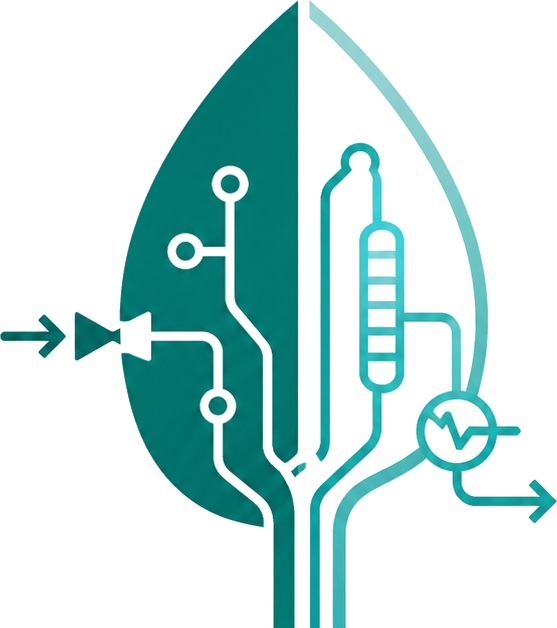
\includegraphics[height=4.0cm]{../gui/public/logo2-mark.png}\\[0.8cm]
  {\Huge\bfseries\sffamily Choupo}\\[0.35cm]
  {\Large\sffamily The Open Source Chemical Process Simulator}\\[1.3cm]
  {\Huge\bfseries\sffamily #1}\\[0.7cm]
  {Version 2607}\\[0.1cm]
  {30 June 2026}
  \end{center}
  \end{titlepage}

  \clearpage
  \thispagestyle{empty}
  \vspace*{1.2cm}
  \noindent Copyright \textcopyright{} 2026 \manualauthors.\\[0.3cm]
  \noindent Authors: \manualauthors.\\[0.3cm]
  \noindent This work is licensed under a Creative Commons
  Attribution-ShareAlike 4.0 International License.\\[0.3cm]
  \noindent Code examples, Choupo case files, and other machine-readable
  examples are licensed under GPL-3.0-or-later.\\[0.3cm]
  \noindent Typeset in \LaTeX.

  \vspace{1.0cm}
  \noindent\rule{\linewidth}{0.3pt}
  \noindent\footnotesize\textit{Acknowledgment.}\quad Choupo was conceived and
  architected by V\'{\i}tor Geraldes. Substantial parts of the initial
  implementation, documentation, and tutorial corpus were produced with
  assistance from Anthropic Claude Code using Claude Opus/Fable models. This
  guide is published under human curation, review, and editorial responsibility
  by \manualauthors.

  \clearpage
  \markboth{License}{License}
  \section*{License}
  \lstinputlisting[
    basicstyle=\ttfamily\tiny,
    frame=none,
    backgroundcolor=\color{white},
    breaklines=true,
    columns=fullflexible
  ]{cc-by-sa-4.0.txt}

  \clearpage
  \markboth{Trademarks}{Trademarks}
  \section*{Trademarks}
  #2
  \clearpage
}

\usepackage{adjustbox}

% ---------------------------------------------------------------------------
%  Per-tutorial entry macros (the generated files use these).
% ---------------------------------------------------------------------------
\newcommand{\tutentry}[2]{%
  \par\medskip\noindent
  \addcontentsline{toc}{subsubsection}{\texttt{#1}}%
  {\large\bfseries\texttt{#1}}\\[1pt]
  {\footnotesize\color{gray}\texttt{#2}}\par\smallskip}
\newcommand{\tutwhat}[1]{\noindent\textbf{What it does:}\ #1\par\smallskip}
\newcommand{\tutstory}[1]{\noindent{\small #1}\par}
\newenvironment{tutscheme}{%
  \par\smallskip\noindent\begin{center}\begin{adjustbox}{max width=\linewidth, max height=7cm}}{%
  \end{adjustbox}\end{center}\par\smallskip}
\newenvironment{tutnarrative}{\par\noindent\textbf{The story:}\ \small}{\par\normalsize\smallskip}
\newcommand{\tutreadme}[1]{\par\noindent{\small\emph{#1}}\par}
\newenvironment{tutgolden}{%
  \par\smallskip\noindent\textbf{What to expect (golden-locked):}\par\nopagebreak\vspace{2pt}
  \begin{footnotesize}\begin{tabular}{@{}llll@{}}\toprule
  kind & unit/stream & key & expected \\ \midrule}{%
  \bottomrule\end{tabular}\end{footnotesize}\par\medskip}
\newcommand{\goldrow}[4]{\texttt{#1} & \texttt{#2} & \texttt{#3} & \texttt{#4} \\}
\newcommand{\goldmore}[1]{\multicolumn{4}{l}{\emph{\dots and #1 more reference values in the case's \file{expected}.}} \\}

% The theory hook: the generated files call \grouptheory{<group>} right after
% each group heading; groups with a hand-written theory block get one via the
% \deftheory mechanism below, the rest expand to nothing.
\makeatletter
\newcommand{\grouptheory}[1]{\@ifundefined{grouptheory@#1}{}{\csname grouptheory@#1\endcsname}}
\newcommand{\deftheory}[2]{\expandafter\def\csname grouptheory@#1\endcsname{%
  \begin{theorybox}#2\end{theorybox}}}
\makeatother
\newenvironment{theorybox}{%
  \par\medskip\noindent\begin{minipage}{\linewidth}\small
  \textbf{The theory you need.}\ }{\end{minipage}\par\medskip}
\newcommand{\theoryref}[1]{\emph{Full derivation: Theory Guide, #1.}}

% ===========================================================================
%  THE THEORY BLOCKS -- hand-written, condensed, with the load-bearing
%  equations; each ends with a pointer to the full Theory Guide chapter.
%  (The per-tutorial text below each block is GENERATED from the cases' own
%  headers -- regenerate with bin/curate/gen_tutorials_guide.py.)
% ===========================================================================

\deftheory{flash}{%
An isothermal flash splits a feed of composition $z_i$ into vapour $y_i$ and
liquid $x_i$ at fixed $(T,P)$.  Phase equilibrium is $y_i = K_i x_i$ with
$K_i = \gamma_i P_i^{\mathrm{sat}}/P$ ($\gamma$--$\varphi$ formulation), and
the vapour fraction $\beta$ solves the Rachford--Rice equation
\[ \sum_i \frac{z_i\,(K_i - 1)}{1 + \beta\,(K_i - 1)} = 0, \]
monotone in $\beta$ -- Newton converges in a handful of iterations, all of
them visible at verbosity 3.  Expect: a bubble point when the equation's
root hits $\beta = 0$, a dew point at $\beta = 1$, and non-ideal systems
($\gamma_i \ne 1$: NRTL/Wilson/UNIQUAC/UNIFAC) bending $K_i$ with
composition.  Liquid--liquid and three-phase cases replace
successive-substitution with direct Gibbs-energy minimisation (the symmetric
$\gamma$-model trap: Newton collapses onto the trivial $K=1$ root).
\theoryref{the VLE and flash chapters}}

\deftheory{distillation}{%
A column is $N$ flash stages coupled by counter-current flows.  Each stage
obeys MESH equations: Material balance, Equilibrium ($y_i = K_i x_i$),
Summation ($\sum y = \sum x = 1$), and Heat balance.  Choupo ships two
solution strategies, selectable per column: Wang--Henke (bubble-point,
solving the tridiagonal material balances stage by stage; robust for
near-ideal systems, slow near azeotropes) and \code{simultaneous} (one
Newton on ALL the MESH residuals; $\sim$5--6 iterations even through
azeotropes).  Expect: reflux and boilup set the split; a minimum reflux
below which no stage count reaches the spec; and azeotropes as fixed points
no column can cross ($x_D$ pinned at the azeotropic composition).
\theoryref{the distillation chapter (McCabe--Thiele + MESH)}}

\deftheory{reactor}{%
Three idealised steady reactors.  Conversion reactor: stoichiometry only,
$n_{\mathrm{out}} = n_{\mathrm{in}} + \nu\,\xi$, duty from the ONE enthalpy
base $\Delta H_{\mathrm{rxn}}(T) = \sum_i \nu_i h_i(T)$ (formation datum --
no separate ``heat of reaction'' input, and any dict override is
cross-checked aloud).  CSTR: outlet at reactor conditions with rate
$r(c_{\mathrm{out}},T)$, so $F\,(c_{\mathrm{in}} - c_{\mathrm{out}}) =
r\,V$.  PFR: the same rate integrated along the volume,
$\mathrm{d}F_i/\mathrm{d}V = \nu_i\,r$.  Arrhenius kinetics
$k = A\,T^b e^{-E_a/RT}$, orders from the dict, reverse rates from the
equilibrium constant (thermo-consistent by construction).  Expect: CSTR
conversion below PFR at equal volume (back-mixing), exponential $T$
sensitivity, and equilibrium limits the kinetics can approach but never
cross. \theoryref{the reaction-engineering chapter}}

\deftheory{reactors}{%
Batch reactors integrate $\mathrm{d}n_i/\mathrm{d}t = \nu_i\,r\,V$ from a
charged initial state -- no in/out flows; time replaces residence time.
Adiabatic runs couple the energy balance
$\sum_i n_i \bar{c}_{p,i}\,\mathrm{d}T/\mathrm{d}t = -\Delta H_{\mathrm{rxn}} r V$,
so composition and temperature evolve together.  Stiffness appears the
moment fast and slow reactions coexist (radical chains: $\mu$s radical
lifetimes vs ms induction) -- the explicit RK4 integrator then needs
$\Delta t$ at the FASTEST scale or blows up, while Rosenbrock23 (L-stable,
linearly implicit) steps at the scale of the SOLUTION.  The stiffness ratio
is printed; watch it. \theoryref{the batch/ODE chapter}}

\deftheory{gibbs}{%
Equilibrium without a mechanism: minimise total Gibbs energy
$G = \sum_i n_i\,\mu_i$ over ALL species subject to elemental balances
$\mathbf{A}\,\mathbf{n} = \mathbf{b}$ (Lagrange multipliers per element --
printed as $\lambda_E$, the element potentials).  The species list in the
dict IS the model: what you include can form; what you omit cannot.  With
enough species this reproduces flame temperatures and radical pools with no
kinetics at all: expect the adiabatic flame temperature to land within a few
K of literature when radicals (H, O, OH\dots) are IN the pool, and to
overshoot by $\sim$100--250\,K when they are not (dissociation is
endothermic).  Above $\sim$1500\,K the catalogue's polynomial $c_p$ fits
extrapolate WRONG -- combustion cases carry case-local NASA-7 overrides,
and the case headers say so.

\medskip
\emph{Equilibrium maps.}  Sweeping the Gibbs solve over a $T\times P$ grid
gives an equilibrium map -- iso-lines of a product fraction over the
operating plane -- which shows why an industrial reactor fixes $T$ and $P$
in a narrow window (equilibrium wants one corner, the catalyst works in
another; the gap is the compromise).  The \code{temperatureApproach}
$\Delta T$ evaluates the \emph{reaction} equilibrium at $T+\Delta T$ while
enthalpy and the energy balance stay at the physical $T$ -- an empirical,
calibrated closeness-to-equilibrium knob (never predicted).
\emph{Gradeable exercise (ammonia):} on \code{nh3\_equilibrium\_map},
at $P = 200$\,bar and $\Delta T = 0$, find the temperature at which the
equilibrium NH$_3$ mole fraction crosses 30\,\%; report $T$ to the grid
resolution and verify against the case's anchor KPIs.  Unique because the
fraction is monotone in $T$ at fixed $P$. \theoryref{the Gibbs-equilibrium
chapter, \S equilibrium maps}}

\deftheory{flowsheets}{%
Recycle turns a flowsheet into a fixed-point problem: guess the tear stream,
march the units, compare.  Successive substitution converges linearly (and
diverges past unit gain); Wegstein accelerates it; Newton-on-tears solves
the tear residuals with a Jacobian.  Choupo announces the tear choice, every
iteration's residual, and any bound that binds -- no silent crutch.  Expect:
purge streams controlling inert build-up (close the loop with no purge and
watch the accumulation), and convergence behaviour that CHANGES with the
tear location. \theoryref{the flowsheet-convergence chapter}}

\deftheory{evaporation}{%
An evaporator boils solvent off a solution.  Two pieces of physics beyond a
flash: boiling-point elevation, $T_{\mathrm{boil}} =
T_{\mathrm{sat}}(P) + \mathrm{BPE}$ with the BPE from the electrolyte
activity of water ($\ln a_w = -\varphi\,\nu\,m\,M_w/1000$); and the heat of
dilution/concentration (the relative apparent molar enthalpy
$L_\varphi(m,T)$) entering the duty.  Expect: the BPE to GROW as the brine
concentrates, steam economy below 1 for a single effect, and -- for NaCl --
the full Silvester--Pitzer $T$-dependence of $\gamma_\pm$ shaping the answer
between 25 and 200$^\circ$C. \theoryref{the electrolyte chapters}}

\deftheory{crystallisation}{%
Crystallisation removes solute when the solution crosses saturation:
$m > m_{\mathrm{sat}}(T)$, with $K_{\mathrm{sp}}(T)$ from
$\Delta G_{\mathrm{diss}}$ and its $T$-dependence from
$\Delta H_{\mathrm{diss}}$ (van 't Hoff).  The heat of crystallisation is
ION-DERIVED -- $\Delta H_{\mathrm{cryst}} = -(\Delta H_{\mathrm{soln}}^\infty
+ \bar{L}_2(m_{\mathrm{sat}}))$ -- never a stored constant (a solid's
formation enthalpy is $\sum \nu_i h_{f,i}^{\mathrm{aq}} -
\Delta H_{\mathrm{soln}}$, derived, single-sourced).  Antisolvent cases add
the mixed-solvent electrolyte model (eNRTL): ethanol drops the dielectric
constant, $\gamma_\pm$ rises, salt crashes out.  Expect supersaturation as
the driving force and yields set by the solubility curve, not the kinetics
(these cases are equilibrium-staged). \theoryref{the crystallisation +
electrolyte-enthalpy chapters}}

\deftheory{membranes}{%
Solution-diffusion (Wijmans \& Baker 1995): inside a dense membrane the
pressure is uniform, so permeation is concentration-driven.  Linearised:
$J_w = A_w(\Delta P - \Delta\pi)$ and $J_s = B_s(c_m - c_p)$ -- water driven
by NET pressure, solute blind to pressure; $(A_w, B_s)$ are MATERIAL
constants from \file{data/standards/assets/}.  Concentration polarisation
(film model) makes the wall concentration $c_m = c_b\,e^{J_w/k}$ exceed the
bulk -- the flux--polarisation--osmotic feedback is THE nonlinearity of
RO/NF, solved per module segment.  Expect: rejection improving with
pressure ($c_p = B_s c_m/(J_w + B_s)$), polarisation eating driving force at
high flux, and charged-membrane (Donnan) effects on multivalent ions that
plain solution-diffusion cannot see -- that is what the DSPM-DE sibling
model is for. \theoryref{the membrane chapter}}

\deftheory{electrolyte}{%
Ions interact at long range (Debye--H\"uckel, $\sqrt{I}$ law) and short
range (ion--ion, ion--solvent).  Choupo's ladder: Davies (charge-only,
$I \le 0.5$), single-salt Pitzer ($\beta_0,\beta_1,C^\varphi$; to
$I \sim 6$, and with the Silvester--Pitzer $T$-functions to 300$^\circ$C),
multi-ion Pitzer--HMW (per-ion, mixing terms $\theta,\psi$ -- seawater-class
brines), and eNRTL (local-composition; single-salt, mixed-solvent, and the
2009 symmetric multi-salt with both published and Gibbs--Duhem-consistent
formulations).  Speciation solves mass action + charge balance by Newton in
log-molality space; saturation indices $\mathrm{SI} =
\log(\mathrm{IAP}/K_{\mathrm{sp}})$ flag scaling.  Expect: models to
DISAGREE above their validity ($\gamma$ divergence is the lesson, e.g.\
Davies vs Pitzer at RO recoveries), and every activity model to announce
itself. \theoryref{the electrolyte + speciation chapters}}

\deftheory{combustion}{%
Radical chain chemistry: initiation creates the first radicals (slow --
$\mathrm{H_2 + M}$, $E_a \sim 105$\,kcal), branching multiplies them
($\mathrm{H + O_2 \to O + OH}$: one in, two out), termination removes them.
Ignition is the race between branching and termination; the induction time
is set by the SLOW build-up, then heat release runs away.  Rate constants
$k = A T^b e^{-E_a/RT}$ come VERBATIM from cited mechanisms (GRI-Mech 3.0,
\'O Conaire 2004, Glarborg 2018) in their native units -- the engine
converts and announces.  Reverse rates from equilibrium: the kinetic
end-state must land on the Gibbs equilibrium (the two-engine handshake the
NOx tutorial pins at 98.9\,\%).  Expect stiffness ratios of $10^6$--$10^8$
(use Rosenbrock23), ignition delays in $\mu$s validated against shock-tube
data, and thermal NO forming over SECONDS -- the timescale gap behind
quench-based NOx control. \theoryref{the combustion/kinetics chapter}}

\deftheory{steam}{%
Water/steam properties from IAPWS-IF97: regions (liquid, vapour,
supercritical), $T_{\mathrm{sat}}(P)$, and $h(T,P)$/$s(T,P)$ from the
dimensionless Gibbs functions.  Power cycles are enthalpy bookkeeping around
them: pump work $\approx v\,\Delta P$, turbine work from isentropic
expansion $\times$ efficiency, cycle efficiency $\eta = W_{\mathrm{net}}/Q_{\mathrm{in}}$
bounded by Carnot. \theoryref{the steam/power chapter}}

\deftheory{power}{%
Gas (Brayton) and steam (Rankine) cycles, alone and combined.  Compressor
and turbine hardware is specified by SHAFT WORK and isentropic efficiency --
outlet pressure is a RESULT, not an input (the anti-DesignSpec credo).
Expect: pressure ratio setting Brayton efficiency, the combined cycle's gain
coming from bottoming the gas turbine's exhaust exergy, and every energy
flow visible in the ledger. \theoryref{the power-cycle chapter}}

\deftheory{heat}{%
Heat exchange couples streams without mixing them: $Q = U\,A\,\Delta
T_{\mathrm{lm}}$, effectiveness-NTU when outlets are unknown.  Utilities
(steam levels, cooling water) are allocated by temperature level -- a
reboiler cannot be heated by a colder utility, and the allocator says which
level it picked.  Heat-links (forward and feedback) couple distant units
into an energy tear the solver converges like any recycle.  Pinch analysis
finds the minimum utilities the composite curves allow.

\medskip
\emph{Exchanger DESIGN vs rating.}  A shell-and-tube poses two inverse
questions: RATE it (geometry given $\to$ find $U$, area, $\Delta P$, duty --
\code{model geometry;}) or DESIGN it (duty given $\to$ size the geometry --
\code{model design;}).  $U$ is BUILT from the two film coefficients
(Gnielinski tube, Kern shell) and the wall; the pressure drop (Kern both
sides) is the duty-vs-pumping half a real design lives by.  The standard
workflow -- establish the duty, THEN design, THEN rate, never invent the
geometry up front -- is walked end-to-end in the two-part sequence
\code{hxWorkflow1\_design\_from\_duty} $\to$ \code{hxWorkflow2\_rate\_designed},
and the design ends in a printable datasheet (GUI: the unit panel).
\theoryref{the heat-integration chapter, \S heat-exchanger design}}

\deftheory{estimate}{%
When a compound is missing, group contribution builds it: Joback sums
first-order group increments into $T_b, T_c, P_c, V_c, \Delta H_f^\circ,
\Delta H_{\mathrm{vap}}, c_p^{\mathrm{ig}}(T)$; Lee--Kesler closes $\omega$
from $(T_b, T_c, P_c)$; Ambrose--Walton gives $P^{\mathrm{sat}}(T)$ from
corresponding states; Rackett the liquid volume.  The estimate is a
PROPOSAL: a \file{.dat} you review against any reference data and promote
by hand -- the engine never estimates at runtime.  Molecular structure is
IDENTITY: components carry \code{jobackGroups\{\}} in their own record, and
\code{bin/estimate <name>} is the one-command curation act.  Expect
few-percent errors on criticals (and the guide's worked example shows
them), weaker $T_b$ for hydrogen-bonded species, and polymers via van
Krevelen / Yang on the repeat unit. \theoryref{the estimation chapter of
the Props Guide}}

\deftheory{scan}{%
Property scans sweep a model across $T$, $P$ or composition and plot what
the thermodynamics DOES: $P^{\mathrm{sat}}(T)$ curves, $\gamma_\pm(m)$,
VLE envelopes, ternary diagrams, phase boundaries.  Nothing is fitted --
these ops answer ``how does the selected model behave?'', the SEE step of
the props loop (CREATE $\to$ SEE $\to$ TEST $\to$ FIT $\to$ PROMOTE).
Expect model disagreements to be VISIBLE (overlay two methods and look), and
every curve exportable as CSV next to the case. \theoryref{the Props Guide}}

\deftheory{thermo}{%
Consistency tests interrogate DATA, not models: the van Ness point test
checks measured $(x,y,T,P)$ sets against the Gibbs--Duhem constraint
(residuals in $\ln(\gamma_1/\gamma_2)$); Herington's area test is its
integral cousin.  A dataset that fails is not ``bad'' -- the test says WHERE
and HOW MUCH, and the fit that follows should weight accordingly.  Expect
plain-language verdicts with severity, not a pass/fail stamp.
\theoryref{the consistency chapter of the Props Guide}}

\deftheory{compare}{%
Method comparison runs the SAME property through different models
side-by-side -- UNIFAC vs NRTL, Joback vs measured, ideal vs EOS.  The gap
between curves IS the modelling uncertainty; picking a method is a decision
the case author owns, made with eyes open. \theoryref{the Props Guide}}

\deftheory{still}{%
A batch still is Rayleigh distillation: $\mathrm{d}(n\,x_i)/\mathrm{d}t =
-\dot{V} y_i$ with $y_i$ in equilibrium with the pot -- the pot composition
DRIFTS as the light component leaves (contrast the steady column, where
stages hold profiles constant).  Expect the distillate to start rich and
fade, and the recipe layer (charge, heat, switch receivers) to drive the
run. \theoryref{the batch-distillation section}}

\deftheory{recipes}{%
A recipe is time-triggered discrete control over batch units: charge,
heat/cool, hold, transfer, sample.  Between events the DAE integrator runs;
at each event the state jumps (a transfer moves holdup between vessels).
Expect exact event times on the trajectory and holdup bookkeeping that
conserves mass across transfers.}

\deftheory{adsorber}{%
Adsorption in a vessel or a bed: the isotherm $q^{*}(T,p)$ (Langmuir
$q = q_{\max} b p/(1+bp)$, van't Hoff $b(T)$) is the curated PAIR datum;
the LDF rate $\mathrm{d}q/\mathrm{d}t = k\,(q^{*} - q)$ carries the
EQUIPMENT datum $k$ (this particle, this bed -- it lives in the case, never
the catalogue).  Work the cases as a staircase.  \code{batch09}: a closed
vessel relaxes to the inventory equilibrium -- one algebraic root, pinned
independently of the run.  \code{batch10}: two species compete for the
same sites (extended Langmuir) -- the selectivity is an equilibrium
statement, and the model's Gibbs--Duhem inconsistency for unequal
$q_{\max}$ is declared, not hidden.  \code{batch11}: in the Henry limit
the whole vessel is LINEAR and the integrator must match
$q_\infty(1-e^{-k_{\mathrm{eff}}t})$ to $10^{-8}$ -- the analytic gate.
\code{batch12}: declaring the headspace pressure AND the inventory
over-specifies a closed ideal-gas vessel -- the contradiction FATALs;
$P$ is a result.  \code{batch13}: the fixed bed -- the stoichiometric
time $t_{\mathrm{st}} = (L/u)(\varepsilon + \rho_b q^{*}/c_{\mathrm{in}})$
is announced BEFORE integration, breakthrough spreads around it, and the
constant-$u$ closure's fabricated carrier is printed, pinned and
discounted: the DECLARED model residual is itself the lesson.
\code{batch14}/\code{batch15} are the numerical hygiene: pure transport
vs the analytic advection--dispersion solution, and the mesh study that
earns $N = 100$. \theoryref{the adsorption chapter}}

\deftheory{adsorption}{%
The isotherm bench: evaluating a curated adsorption-equilibrium record
(Henry-limit, saturation, pin and unit-invariance gates run aloud) and
REGRESSING one from data -- the multi-temperature van't Hoff Langmuir fit
with identifiability verdicts: single-$T$ data refuses $\Delta
H_{\mathrm{ads}}$, Henry-regime data yields only the product $q_{\max}
b$, and a non-converged fit refuses its verdict by name.
\theoryref{the adsorption chapter}}

\deftheory{absorption}{%
Gas absorption transfers a solute from gas to liquid across stages; Henry's
law ($p_i = H_i x_i$) anchors the equilibrium at dilution.  Expect the
L/G ratio to control the operating line's slope, and a minimum solvent rate
at the pinch with the equilibrium line.
\theoryref{the absorption section}}

\deftheory{solids}{%
Solids carry mass and enthalpy without VLE: crystallisers, dryers, cyclones,
gas--solid splitters.  A dryer's air is a REAL stream (two inlets, adiabatic
mixing, outlet humidity from the psychrometrics); a cyclone's cut size comes
from the selected model (Lapple\dots Muschelknautz).  Expect solid streams
flagged separately ($F_{\mathrm{solid}}$) and energy balances that close
across phase change.}

\deftheory{hydraulics}{%
Pressure drop and flow distribution: Darcy--Weisbach with friction factors,
fittings as equivalent lengths, pump curves against system curves.  Expect
the operating point at the curves' intersection.}

\deftheory{utilities}{%
Utility streams (steam levels, cooling water, refrigerants, electricity)
carry duty into and out of the plant at declared temperature levels and
prices; allocation is by $T$-level feasibility, announced.}

\deftheory{rotating}{%
Compressors, turbines, pumps: specified by shaft work $W_s$ and isentropic
efficiency $\eta_s$; the outlet state follows from
$h_{\mathrm{out}} = h_{\mathrm{in}} + W_s/\dot{n}$ with the isentropic
reference path.  Outlet pressure is a RESULT (hardware, not a spec).}

\deftheory{optimisation}{%
The outer driver wraps the whole simulation in $f(\mathbf{x})$: sweeps map
it, Nelder--Mead descends it, parameter estimation fits it to data
(Levenberg--Marquardt, with identifiability diagnostics --
$\chi^2_{\mathrm{red}}$, correlation, conditioning).  Expect every function
evaluation to be a full, honest flowsheet pass.}

\deftheory{molecular}{%
Molecular activity models on display: NRTL/Wilson/UNIQUAC correlate binary
$\gamma$'s from pair parameters; UNIFAC PREDICTS them from group
counts.  Expect UNIFAC within a few percent of fitted models for families it
was trained on -- and to be honestly worse outside them.
\theoryref{the activity-model chapter}}

\deftheory{esterification2sector}{%
The self-contained two-sector demo: reaction (esterification CSTR) +
separation, fractal case layout (each sector its own folder), recycle
between them.  The showcase for the dignified-unit layout.}

\deftheory{twoSectorDemo}{%
The zippable two-sector demonstration plant -- the case used to rehearse
the online landing.  Same physics as the esterification demo.}

\deftheory{ChemicalPlantTutorial}{%
The full multi-sector plant showcase: feed treatment, reaction, separation,
utilities -- the fractal flowsheet at its largest, run-only (no golden), for
reading and dissecting rather than reproducing numbers.}

\deftheory{polycaprolactonePlant}{%
Ring-opening polymerisation plant: monomer to polycaprolactone with
step-growth KPIs (Carothers, Flory) on the PFR, polymer properties from
group contribution on the repeat unit.}

\deftheory{userops}{%
User-defined operations: the extension seam.  A custom property op or unit
compiled into the binary via the explicit factory -- the tutorial shows the
registration pattern (\code{registerBuiltins}) end to end.}

\deftheory{economics}{%
Sizing (stirred tanks, shell-and-tube areas) feeds costing (Guthrie
modules); prices are CASE data (\file{constant/economics}, dated and
cited) -- the engine refuses to invent a price.  Expect honest refusal when
a price is missing, never a silent default.}

% ===========================================================================
\title{}
\author{}
\date{}

\begin{document}

\manualfrontmatter{Tutorials Guide}{
Choupo is a trademark of TalentGround Lda.

Anthropic, Claude, and Claude Code are trademarks or registered trademarks of
Anthropic, PBC.
}

{\small\setcounter{tocdepth}{3}\setcounter{secnumdepth}{0}\tableofcontents}
\clearpage

% =====================================================================
\section*{How to use this guide}
\addcontentsline{toc}{section}{How to use this guide}

Every Choupo tutorial is a complete, runnable case:
\begin{verbatim}
   source etc/bashrc
   runCase tutorials/<category>/<group>/<name>
\end{verbatim}
This guide gives each tutorial the CONTEXT the case file cannot: the theory
block at the head of each group states the physics and the equations you
need (condensed -- the Theory Guide carries the full derivations), and each
entry tells you \textbf{what the case does} and \textbf{what to expect}
before you run it.  The per-tutorial text is assembled from the cases' own
headers -- the case file is always the source of truth, and reading it IS
part of the exercise.

Three reading rules:
\begin{enumerate}[leftmargin=*,nosep]
  \item \textbf{Run first, read second, re-run third.}  The log at
        verbosity 3 shows every Newton iteration, every K-value, every
        announcement -- the glass box is the point.
  \item \textbf{Expect the announcements.}  Choupo never silently helps:
        initial guesses, bounds that bind, model fallbacks, unit overrides
        -- all are printed.  If a run is quiet about something, it did not
        happen.
  \item \textbf{Golden numbers are commitments.}  Cases carrying an
        \file{expected} file pin their KPIs; the validation AADs quoted in
        the entries are locked by the regression suite and re-verified on
        every change.
\end{enumerate}

% =====================================================================
\section*{Learning paths}
\addcontentsline{toc}{section}{Learning paths}

\paragraph{The MCFT path (computational transfer phenomena).}
Start with \texttt{flash01\_benzene\_toluene} (the Rachford--Rice loop,
visible), then \texttt{flash} non-ideal cases (activity models bend the
K-values), \texttt{distillation} (stages couple; Wang--Henke vs
simultaneous), one \texttt{flowsheets} recycle case (tears and convergence),
and close with a \texttt{gibbs} flame (equilibrium without mechanism).
Then the batch side: an \texttt{ignition} case for stiffness -- run the
\texttt{\_rk4} twin and watch the explicit method die -- and a \texttt{ctrl}
loop for feedback.

\paragraph{The electrolytes path.}
\texttt{pitzer01\_nacl} ($\gamma_\pm$, $\varphi$, $a_w$ of one salt), then
\texttt{pitzer\_gamma\_hamer\_wu} (the catalogue vs NBS data, zero refit),
\texttt{pitzer\_nacl\_sp77\_hot} (temperature, to 200$^\circ$C),
speciation (\texttt{scaling} cases: SI, pH, Davies-vs-Pitzer forking an
engineering answer), the eNRTL series
(\texttt{enrtl\_mixed\_nacl\_ethanol\_esteso} mixed-solvent;
\texttt{enrtl\_multisalt\_nacl\_kcl} two salts, two formulations, an
experimental verdict), and the process payoff: evaporators and
crystallisers where all of it sets duties and yields.

\paragraph{The combustion path.}
\texttt{gibbs06\_h2\_flame\_radicals} (the radical pool at equilibrium; the
$c_p$ extrapolation trap), \texttt{ignition01\_h2o2} (GRI kinetics, the
stiffness lesson via the \texttt{\_rk4} twin), \texttt{ignition02\_h2air\_slack}
(quantitative: $\tau_{\mathrm{ign}}$ vs shock-tube data),
\texttt{nox01\_zeldovich\_postflame} (thermal NO; kinetics meets Gibbs at
98.9\,\%).

\paragraph{The props-bench path.}
\texttt{estimate\_acetone} (CREATE: groups $\to$ constants, error shown),
a \texttt{scan} case (SEE), \texttt{vle01\_consistency} (TEST the data),
a \texttt{fit} case (Levenberg--Marquardt with identifiability), then the
promote-and-use loop into a steady case.  The Props Guide is this path's
companion.

% =====================================================================
\clearpage
\section*{Category I: Steady-state flowsheets (choupoSolve)}\addcontentsline{toc}{section}{Category I: Steady-state flowsheets (choupoSolve)}\markboth{Steady-state flowsheets}{Steady-state flowsheets}
Solved as one nonlinear system $F(\mathbf{x}) = \mathbf{0}$: units in
sequence, recycles as tears, everything announced.
% GENERATED by bin/curate/gen_tutorials_guide.py -- DO NOT EDIT BY HAND.
% Assembled from each case's controlDict description + header comment.

\subsection{absorption}
\grouptheory{absorption}
\clearpage
\tutentry{absorber01\_NH3\_water}{tutorials/steady/absorption/absorber01\_NH3\_water}
\begin{tutscheme}
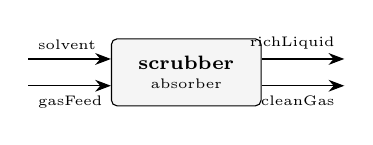
\begin{tikzpicture}[>={Stealth[length=2mm]}, every node/.style={font=\scriptsize}]
  \node[draw, rounded corners=2pt, align=center, minimum width=1.9cm, minimum height=0.85cm, fill=black!4] (scrubber) at (0.0,-0.0) {\textbf{scrubber}\\[-1pt]{\tiny absorber}};
  \draw[->] ($(scrubber.west)+(-1.05,-0.17)$) -- ($(scrubber.west)+(0,-0.17)$) node[at start, below, font=\tiny, anchor=north west] {gasFeed};
  \draw[->] ($(scrubber.west)+(-1.05,0.17)$) -- ($(scrubber.west)+(0,0.17)$) node[at start, above, font=\tiny, anchor=south west] {solvent};
  \draw[->] ($(scrubber.east)+(0,-0.17)$) -- ($(scrubber.east)+(1.05,-0.17)$) node[at end, below, font=\tiny, anchor=north east] {cleanGas};
  \draw[->] ($(scrubber.east)+(0,0.17)$) -- ($(scrubber.east)+(1.05,0.17)$) node[at end, above, font=\tiny, anchor=south east] {richLiquid};
\end{tikzpicture}
\end{tutscheme}
\tutwhat{NH3 absorption from air into water (Kremser, 6 stages)}
\begin{tutnarrative}
- Choupo -$\ast$--------------------------------$\ast$ | \textbackslash\{\}|/ C hemicals | Choupo: open-source, glass-box simulation | | \textbackslash\{\}\textbackslash\{\}|// H eat-transfer | Version: Choupo-dev | | \textbackslash\{\}\textbackslash\{\}\textbackslash\{\}|/// O perations | Website: https://choupo.org | | \textbackslash\{\}\textbackslash\{\}|// U nits | Licence: GPL-3.0-or-later | | \textbackslash\{\}|/ P roperties | Tutorial case file -- part of Choupo | | | O ptimization | |

\end{tutnarrative}
\begin{tutgolden}
\goldrow{stream}{cleanGas}{F}{0.0259019084984}
\goldrow{stream}{gasFeed}{F}{0.0277777777778}
\goldrow{stream}{richLiquid}{F}{0.043542535946}
\goldrow{stream}{solvent}{F}{0.0416666666667}
\goldrow{kpi}{scrubber}{A\_N2}{0.00225907961951}
\goldrow{kpi}{scrubber}{A\_NH3}{1.53522727273}
\goldrow{kpi}{scrubber}{F\_cleanGas}{0.0259019084984}
\goldrow{kpi}{scrubber}{F\_richLiquid}{0.043542535946}
\goldrow{kpi}{scrubber}{K\_N2}{663.987221631}
\goldrow{kpi}{scrubber}{K\_NH3}{0.977054034049}
\goldrow{kpi}{scrubber}{L\_in}{0.0416666666667}
\goldrow{kpi}{scrubber}{L\_over\_V}{1.5}
\goldrow{kpi}{scrubber}{V\_in}{0.0277777777778}
\goldrow{kpi}{scrubber}{recovery\_N2}{0}
\goldmore{2}
\end{tutgolden}

\clearpage
\tutentry{absorption01\_CO2\_water}{tutorials/steady/absorption/absorption01\_CO2\_water}
\begin{tutscheme}
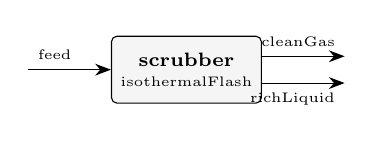
\begin{tikzpicture}[>={Stealth[length=2mm]}, every node/.style={font=\scriptsize}]
  \node[draw, rounded corners=2pt, align=center, minimum width=1.9cm, minimum height=0.85cm, fill=black!4] (scrubber) at (0.0,-0.0) {\textbf{scrubber}\\[-1pt]{\tiny isothermalFlash}};
  \draw[->] ($(scrubber.west)+(-1.05,0.00)$) -- ($(scrubber.west)+(0,0.00)$) node[at start, above, font=\tiny, anchor=south west] {feed};
  \draw[->] ($(scrubber.east)+(0,-0.17)$) -- ($(scrubber.east)+(1.05,-0.17)$) node[at end, below, font=\tiny, anchor=north east] {richLiquid};
  \draw[->] ($(scrubber.east)+(0,0.17)$) -- ($(scrubber.east)+(1.05,0.17)$) node[at end, above, font=\tiny, anchor=south east] {cleanGas};
\end{tikzpicture}
\end{tutscheme}
\tutwhat{Single-stage CO2 absorption in water (Henry's law)}
\begin{tutnarrative}
- Choupo -$\ast$--------------------------------$\ast$ | \textbackslash\{\}|/ C hemicals | Choupo: open-source, glass-box simulation | | \textbackslash\{\}\textbackslash\{\}|// H eat-transfer | Version: Choupo-dev | | \textbackslash\{\}\textbackslash\{\}\textbackslash\{\}|/// O perations | Website: https://choupo.org | | \textbackslash\{\}\textbackslash\{\}|// U nits | Licence: GPL-3.0-or-later | | \textbackslash\{\}|/ P roperties | Tutorial case file -- part of Choupo | | | O ptimization | |

\end{tutnarrative}
\begin{tutgolden}
\goldrow{stream}{cleanGas}{F}{0.0183200303715}
\goldrow{stream}{feed}{F}{1.41666666667}
\goldrow{stream}{richLiquid}{F}{1.3983466363}
\goldrow{kpi}{scrubber}{F\_alpha}{1.3983466363}
\goldrow{kpi}{scrubber}{F\_beta}{0.0183200303715}
\goldrow{kpi}{scrubber}{F\_in}{1.41666666667}
\goldrow{kpi}{scrubber}{P}{500000}
\goldrow{kpi}{scrubber}{T}{298.15}
\goldrow{kpi}{scrubber}{V\_over\_F}{0.0129317861446}
\goldrow{kpi}{scrubber}{phaseSet}{0}
\end{tutgolden}

\clearpage
\tutentry{acetone05\_luyben\_absorber}{tutorials/steady/absorption/acetone05\_luyben\_absorber}
\begin{tutscheme}
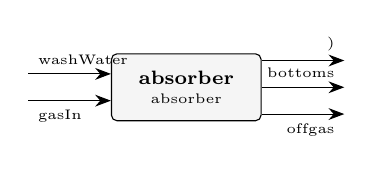
\begin{tikzpicture}[>={Stealth[length=2mm]}, every node/.style={font=\scriptsize}]
  \node[draw, rounded corners=2pt, align=center, minimum width=1.9cm, minimum height=0.85cm, fill=black!4] (absorber) at (0.0,-0.0) {\textbf{absorber}\\[-1pt]{\tiny absorber}};
  \draw[->] ($(absorber.west)+(-1.05,-0.17)$) -- ($(absorber.west)+(0,-0.17)$) node[at start, below, font=\tiny, anchor=north west] {gasIn};
  \draw[->] ($(absorber.west)+(-1.05,0.17)$) -- ($(absorber.west)+(0,0.17)$) node[at start, above, font=\tiny, anchor=south west] {washWater};
  \draw[->] ($(absorber.east)+(0,-0.34)$) -- ($(absorber.east)+(1.05,-0.34)$) node[at end, below, font=\tiny, anchor=north east] {offgas};
  \draw[->] ($(absorber.east)+(0,0.00)$) -- ($(absorber.east)+(1.05,0.00)$) node[at end, above, font=\tiny, anchor=south east] {bottoms};
  \draw[->] ($(absorber.east)+(0,0.34)$) -- ($(absorber.east)+(1.05,0.34)$) node[at end, above, font=\tiny, anchor=south east] {)};
\end{tikzpicture}
\end{tutscheme}
\tutwhat{Luyben's acetone absorber: 9 stages, water washing acetone out of the hydrogen offgas -- against his own acetone and bottoms}
\begin{tutnarrative}
The unit acetone04 was measured FOR. Luyben's absorber washes acetone out of the reactor's hydrogen-rich offgas with water: 9 stages at 1.5 atm, 20 kmol/h of water on top, 39.80 kmol/h of gas at the bottom.

W. L. Luyben, Ind. Eng. Chem. Res. 50 (2011) 1206-1218, DOI 10.1021/ie901923a, Figure 1.

WHAT IS INDEPENDENT HERE, stated before the numbers because the last case in this family had to say the opposite. The gas inlet is Luyben's own ("Gas (to absorber)": 39.80 kmol/h, acetone 0.1147, IPA 0.0033) EXCEPT for its hydrogen and water, which were derived from the gas LEAVING using H2's inertness and a balance. So:

NOT independent -- the outlet H2 and water (the inlet was built from them) INDEPENDENT -- everything about the ACETONE, and the whole bottoms stream. Nothing in 0/ was built from those.

Luyben's answer, for the record, before this case is run:

bottoms 20.05 kmol/h acetone 0.1020 $\to$ 2.045 kmol/h absorbed offgas 39.76 kmol/h acetone 0.0634 $\to$ 2.521 kmol/h lost recovery 2.045 / 4.565 = 44.8 \%

His own table closes on itself to 0.02 \% in both acetone and water, which is two checks on a hand transcription and the reason those numbers are trusted as targets.

WHAT acetone04 PREDICTS FOR THIS UNIT. Measured there, on the same thermodynamics this case runs: gamma\_acetone = 10.27 at 1 mol \% in water and 318 K, giving K = 6.84. A model that holds acetone too weakly in the water will absorb LESS of it than Luyben does. That is the prediction; the run below is the test.

The thermodynamics is PREDICTIVE UNIFAC with H2 authorised outside the activity model -- the same declared package as acetone03, for the same reasons, recorded in constant/thermoPhysPropDict.

\end{tutnarrative}
\begin{tutgolden}
\goldrow{stream}{bottoms}{F}{0.00574366573439}
\goldrow{stream}{gasIn}{F}{0.0110555555556}
\goldrow{stream}{offgas}{F}{0.0108674453767}
\goldrow{stream}{washWater}{F}{0.00555555555556}
\goldrow{kpi}{absorber}{A\_H2}{0.00044153375233}
\goldrow{kpi}{absorber}{A\_acetone}{0.0857422914441}
\goldrow{kpi}{absorber}{A\_isopropanol}{4.51803004485}
\goldrow{kpi}{absorber}{A\_water}{8.0125706439}
\goldrow{kpi}{absorber}{F\_cleanGas}{0.0108674453767}
\goldrow{kpi}{absorber}{F\_richLiquid}{0.00574366573439}
\goldrow{kpi}{absorber}{K\_H2}{1138.10679288}
\goldrow{kpi}{absorber}{K\_acetone}{5.86073166871}
\goldrow{kpi}{absorber}{K\_isopropanol}{0.11122382052}
\goldrow{kpi}{absorber}{K\_water}{0.0627155235376}
\goldmore{12}
\end{tutgolden}

\clearpage
\tutentry{extract01\_ethanol\_water\_benzene}{tutorials/steady/absorption/extract01\_ethanol\_water\_benzene}
\begin{tutscheme}
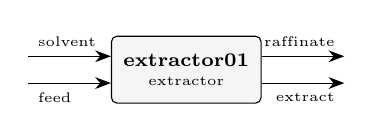
\begin{tikzpicture}[>={Stealth[length=2mm]}, every node/.style={font=\scriptsize}]
  \node[draw, rounded corners=2pt, align=center, minimum width=1.9cm, minimum height=0.85cm, fill=black!4] (extractor01) at (0.0,-0.0) {\textbf{extractor01}\\[-1pt]{\tiny extractor}};
  \draw[->] ($(extractor01.west)+(-1.05,-0.17)$) -- ($(extractor01.west)+(0,-0.17)$) node[at start, below, font=\tiny, anchor=north west] {feed};
  \draw[->] ($(extractor01.west)+(-1.05,0.17)$) -- ($(extractor01.west)+(0,0.17)$) node[at start, above, font=\tiny, anchor=south west] {solvent};
  \draw[->] ($(extractor01.east)+(0,-0.17)$) -- ($(extractor01.east)+(1.05,-0.17)$) node[at end, below, font=\tiny, anchor=north east] {extract};
  \draw[->] ($(extractor01.east)+(0,0.17)$) -- ($(extractor01.east)+(1.05,0.17)$) node[at end, above, font=\tiny, anchor=south east] {raffinate};
\end{tikzpicture}
\end{tutscheme}
\tutwhat{Counter-current LL extraction: recover ethanol from water with benzene}
\begin{tutnarrative}
- Choupo -$\ast$--------------------------------$\ast$ | \textbackslash\{\}|/ C hemicals | Choupo: open-source, glass-box simulation | | \textbackslash\{\}\textbackslash\{\}|// H eat-transfer | Version: Choupo-dev | | \textbackslash\{\}\textbackslash\{\}\textbackslash\{\}|/// O perations | Website: https://choupo.org | | \textbackslash\{\}\textbackslash\{\}|// U nits | Licence: GPL-3.0-or-later | | \textbackslash\{\}|/ P roperties | Tutorial case file -- part of Choupo | | | O ptimization | |

\end{tutnarrative}
\begin{tutgolden}
\goldrow{stream}{extract}{F}{0.0359293973028}
\goldrow{stream}{feed}{F}{0.0277777777778}
\goldrow{stream}{raffinate}{F}{0.0251772962492}
\goldrow{stream}{solvent}{F}{0.0333333333333}
\goldrow{kpi}{extractor01}{F\_extract}{0.0359293973028}
\goldrow{kpi}{extractor01}{F\_feed}{0.0277777777778}
\goldrow{kpi}{extractor01}{F\_raffinate}{0.0251772962492}
\goldrow{kpi}{extractor01}{F\_solvent}{0.0333333333333}
\goldrow{kpi}{extractor01}{P}{101325}
\goldrow{kpi}{extractor01}{T}{298.15}
\goldrow{kpi}{extractor01}{converged}{1}
\goldrow{kpi}{extractor01}{distribution\_benzene}{295.27509389}
\goldrow{kpi}{extractor01}{distribution\_ethanol}{0.555106921422}
\goldrow{kpi}{extractor01}{distribution\_water}{0.00706545462823}
\goldmore{9}
\end{tutgolden}

\clearpage
\tutentry{extraction01\_waterButanol}{tutorials/steady/absorption/extraction01\_waterButanol}
\begin{tutscheme}
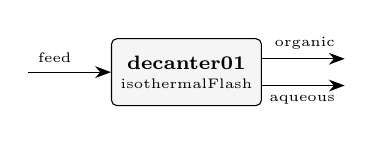
\begin{tikzpicture}[>={Stealth[length=2mm]}, every node/.style={font=\scriptsize}]
  \node[draw, rounded corners=2pt, align=center, minimum width=1.9cm, minimum height=0.85cm, fill=black!4] (decanter01) at (0.0,-0.0) {\textbf{decanter01}\\[-1pt]{\tiny isothermalFlash}};
  \draw[->] ($(decanter01.west)+(-1.05,0.00)$) -- ($(decanter01.west)+(0,0.00)$) node[at start, above, font=\tiny, anchor=south west] {feed};
  \draw[->] ($(decanter01.east)+(0,-0.17)$) -- ($(decanter01.east)+(1.05,-0.17)$) node[at end, below, font=\tiny, anchor=north east] {aqueous};
  \draw[->] ($(decanter01.east)+(0,0.17)$) -- ($(decanter01.east)+(1.05,0.17)$) node[at end, above, font=\tiny, anchor=south east] {organic};
\end{tikzpicture}
\end{tutscheme}
\tutwhat{Water/n-butanol LL flash at 298 K (experimental)}
\begin{tutnarrative}
- Choupo -$\ast$--------------------------------$\ast$ | \textbackslash\{\}|/ C hemicals | Choupo: open-source, glass-box simulation | | \textbackslash\{\}\textbackslash\{\}|// H eat-transfer | Version: Choupo-dev | | \textbackslash\{\}\textbackslash\{\}\textbackslash\{\}|/// O perations | Website: https://choupo.org | | \textbackslash\{\}\textbackslash\{\}|// U nits | Licence: GPL-3.0-or-later | | \textbackslash\{\}|/ P roperties | Tutorial case file -- part of Choupo | | | O ptimization | |

\end{tutnarrative}
\tutreadme{Water + 1-butanol at 25 $^\circ$C and 1 atm. The pair has a well-known liquid-liquid miscibility gap below its upper critical solution temperature (125.5 $^\circ$C), so a feed whose composition lies inside the gap spontaneously splits into two liquid phases. This case feeds a 70/30 water/nButanol mixture (inside the gap) to an isothermal decanter and lets the flash find the two-liquid split.}
\tutreadme{A single feed splits into two liquids, both at 298.15 K, vf = 0:}
\tutreadme{The split is found by Michelsen TPD stability testing (to seed a robust initial guess) followed by direct Gibbs-energy minimisation --- the LL path the engine uses precisely because a Newton/successive-substitution flash on a symmetric $\gamma$-model would collapse to the trivial K = 1 saddle.}
\tutreadme{- phases (...) syntax with TWO liquid phases; - phaseSet LL in the IsothermalFlash; - the Michelsen TPD stability test as the initial-guess generator.}
\tutreadme{- The LL flash reuses the VL solver's printout, so the two liquids are shown under Vapor flow V / Liquid flow L headings (and x/y/K labels). Read them as phase-$\alpha$ (organic) and phase-$\beta$ (aqueous), not as a vapour and a liquid. - The decanter is isothermal and adiabatic in reality (an enthalpy hand-check gives H\_in $\approx$ H\_out), so the physically correct duty is $\approx$ 0. The KPI Q and any utility/cost the run reports for this LL split are a known artifact of the shared flash duty path --- do not cost this unit from them.}
\begin{tutgolden}
\goldrow{stream}{aqueous}{F}{0.0140665296362}
\goldrow{stream}{feed}{F}{0.0277777777778}
\goldrow{stream}{organic}{F}{0.0137112481416}
\goldrow{kpi}{decanter01}{F\_alpha}{0.0140665296362}
\goldrow{kpi}{decanter01}{F\_beta}{0.0137112481416}
\goldrow{kpi}{decanter01}{F\_in}{0.0277777777778}
\goldrow{kpi}{decanter01}{P}{101325}
\goldrow{kpi}{decanter01}{T}{298.15}
\goldrow{kpi}{decanter01}{betaFraction}{0.493604933098}
\goldrow{kpi}{decanter01}{phaseSet}{1}
\end{tutgolden}

\clearpage
\tutentry{stripper01\_NH3\_water}{tutorials/steady/absorption/stripper01\_NH3\_water}
\begin{tutscheme}
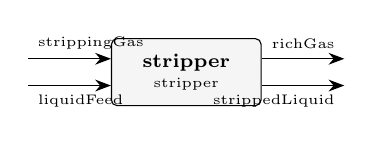
\begin{tikzpicture}[>={Stealth[length=2mm]}, every node/.style={font=\scriptsize}]
  \node[draw, rounded corners=2pt, align=center, minimum width=1.9cm, minimum height=0.85cm, fill=black!4] (stripper) at (0.0,-0.0) {\textbf{stripper}\\[-1pt]{\tiny stripper}};
  \draw[->] ($(stripper.west)+(-1.05,-0.17)$) -- ($(stripper.west)+(0,-0.17)$) node[at start, below, font=\tiny, anchor=north west] {liquidFeed};
  \draw[->] ($(stripper.west)+(-1.05,0.17)$) -- ($(stripper.west)+(0,0.17)$) node[at start, above, font=\tiny, anchor=south west] {strippingGas};
  \draw[->] ($(stripper.east)+(0,-0.17)$) -- ($(stripper.east)+(1.05,-0.17)$) node[at end, below, font=\tiny, anchor=north east] {strippedLiquid};
  \draw[->] ($(stripper.east)+(0,0.17)$) -- ($(stripper.east)+(1.05,0.17)$) node[at end, above, font=\tiny, anchor=south east] {richGas};
\end{tikzpicture}
\end{tutscheme}
\tutwhat{NH3 stripping from water with air (Kremser, 6 stages, warm)}
\begin{tutnarrative}
- Choupo -$\ast$--------------------------------$\ast$ | \textbackslash\{\}|/ C hemicals | Choupo: open-source, glass-box simulation | | \textbackslash\{\}\textbackslash\{\}|// H eat-transfer | Version: Choupo-dev | | \textbackslash\{\}\textbackslash\{\}\textbackslash\{\}|/// O perations | Website: https://choupo.org | | \textbackslash\{\}\textbackslash\{\}|// U nits | Licence: GPL-3.0-or-later | | \textbackslash\{\}|/ P roperties | Tutorial case file -- part of Choupo | | | O ptimization | |

\end{tutnarrative}
\begin{tutgolden}
\goldrow{stream}{liquidFeed}{F}{0.0277777777778}
\goldrow{stream}{richGas}{F}{0.029140357434}
\goldrow{stream}{strippedLiquid}{F}{0.0264151981216}
\goldrow{stream}{strippingGas}{F}{0.0277777777778}
\goldrow{kpi}{stripper}{F\_richGas}{0.029140357434}
\goldrow{kpi}{stripper}{F\_strippedLiquid}{0.0264151981216}
\goldrow{kpi}{stripper}{K\_NH3}{3.62862883208}
\goldrow{kpi}{stripper}{K\_water}{0.170562530402}
\goldrow{kpi}{stripper}{L\_in}{0.0277777777778}
\goldrow{kpi}{stripper}{S\_NH3}{3.62862883208}
\goldrow{kpi}{stripper}{S\_water}{0.170562530402}
\goldrow{kpi}{stripper}{T\_bottom}{313.524974667}
\goldrow{kpi}{stripper}{T\_top}{315.973930965}
\goldrow{kpi}{stripper}{V\_in}{0.0277777777778}
\goldmore{6}
\end{tutgolden}

\subsection{crystallisation}
\grouptheory{crystallisation}
\clearpage
\tutentry{crystalliser01\_sugar}{tutorials/steady/crystallisation/crystalliser01\_sugar}
\tutwhat{Cooling crystalliser: sugar solution 80 $\to$ 20 C, yield by solubility}
\begin{tutnarrative}
- Choupo -$\ast$--------------------------------$\ast$ | \textbackslash\{\}|/ C hemicals | Choupo: open-source, glass-box simulation | | \textbackslash\{\}\textbackslash\{\}|// H eat-transfer | Version: Choupo-dev | | \textbackslash\{\}\textbackslash\{\}\textbackslash\{\}|/// O perations | Website: https://choupo.org | | \textbackslash\{\}\textbackslash\{\}|// U nits | Licence: GPL-3.0-or-later | | \textbackslash\{\}|/ P roperties | Tutorial case file -- part of Choupo | | | O ptimization | |

\end{tutnarrative}
\begin{tutgolden}
\goldrow{stream}{feed}{F}{0.0277777777778}
\goldrow{stream}{magma}{F}{0.0277777777778}
\goldrow{kpi}{cryst}{Q\_removed}{271677.114808}
\goldrow{kpi}{cryst}{T\_op}{293.15}
\goldrow{kpi}{cryst}{c\_sat}{2.026}
\goldrow{kpi}{cryst}{crystal\_flow}{0.564469958333}
\goldrow{kpi}{cryst}{crystal\_mol}{0.00164906487154}
\goldrow{kpi}{cryst}{liquorFlow}{0.0261287129062}
\goldrow{kpi}{cryst}{solute\_dissolved}{0.861767541667}
\goldrow{kpi}{cryst}{solute\_in}{1.4262375}
\goldrow{kpi}{cryst}{yield}{0.395775569169}
\end{tutgolden}

\clearpage
\tutentry{crystalliser02\_msmpr}{tutorials/steady/crystallisation/crystalliser02\_msmpr}
\tutwhat{MSMPR sugar crystalliser: population balance by method of moments}
\begin{tutnarrative}
- Choupo -$\ast$--------------------------------$\ast$ | \textbackslash\{\}|/ C hemicals | Choupo: open-source, glass-box simulation | | \textbackslash\{\}\textbackslash\{\}|// H eat-transfer | Version: Choupo-dev | | \textbackslash\{\}\textbackslash\{\}\textbackslash\{\}|/// O perations | Website: https://choupo.org | | \textbackslash\{\}\textbackslash\{\}|// U nits | Licence: GPL-3.0-or-later | | \textbackslash\{\}|/ P roperties | Tutorial case file -- part of Choupo | | | O ptimization | |

\end{tutnarrative}
\begin{tutgolden}
\goldrow{stream}{feed}{F}{0.0277777777778}
\goldrow{stream}{magma}{F}{0.0277777777778}
\goldrow{kpi}{cryst}{CV}{1}
\goldrow{kpi}{cryst}{L\_dominant}{0.000223952804481}
\goldrow{kpi}{cryst}{L\_meanMass}{0.000298603739308}
\goldrow{kpi}{cryst}{L\_meanNumber}{7.46509348269e-05}
\goldrow{kpi}{cryst}{Q\_removed}{269525.057151}
\goldrow{kpi}{cryst}{T\_op}{293.15}
\goldrow{kpi}{cryst}{c\_sat}{2.026}
\goldrow{kpi}{cryst}{crystal\_flow}{0.396190602513}
\goldrow{kpi}{cryst}{crystal\_mol}{0.00115744690287}
\goldrow{kpi}{cryst}{growthRate}{1.95272330048e-08}
\goldrow{kpi}{cryst}{liquorFlow}{0.0266203308749}
\goldrow{kpi}{cryst}{magmaDensity}{302.920529908}
\goldmore{10}
\end{tutgolden}

\clearpage
\tutentry{crystalliser03\_pbe\_size\_independent}{tutorials/steady/crystallisation/crystalliser03\_pbe\_size\_independent}
\tutwhat{Crystalliser FVM-PBE: sanity vs MSMPR (size-independent growth)}
\begin{tutnarrative}
- Choupo -$\ast$--------------------------------$\ast$ | \textbackslash\{\}|/ C hemicals | Choupo: open-source, glass-box simulation | | \textbackslash\{\}\textbackslash\{\}|// H eat-transfer | Version: Choupo-dev | | \textbackslash\{\}\textbackslash\{\}\textbackslash\{\}|/// O perations | Website: https://choupo.org | | \textbackslash\{\}\textbackslash\{\}|// U nits | Licence: GPL-3.0-or-later | | \textbackslash\{\}|/ P roperties | Tutorial case file -- part of Choupo | | | O ptimization | |

\end{tutnarrative}
\begin{tutgolden}
\goldrow{stream}{feed}{F}{0.0277777777778}
\goldrow{stream}{magma}{F}{0.0277777777778}
\goldrow{kpi}{cryst}{CV}{0.999540291345}
\goldrow{kpi}{cryst}{L\_dominant}{0.000224609375}
\goldrow{kpi}{cryst}{L\_meanMass}{0.000298633437171}
\goldrow{kpi}{cryst}{L\_meanNumber}{7.48298114726e-05}
\goldrow{kpi}{cryst}{Q\_removed}{269576.1605}
\goldrow{kpi}{cryst}{T\_op}{293.15}
\goldrow{kpi}{cryst}{bins}{256}
\goldrow{kpi}{cryst}{c\_sat}{2.026}
\goldrow{kpi}{cryst}{crystal\_flow}{0.400186610054}
\goldrow{kpi}{cryst}{crystal\_mol}{0.00116912099742}
\goldrow{kpi}{cryst}{growthRate\_L0}{1.90635340048e-08}
\goldrow{kpi}{cryst}{liquorFlow}{0.0266086567804}
\goldmore{11}
\end{tutgolden}

\clearpage
\tutentry{crystalliser04\_size\_dependent\_growth}{tutorials/steady/crystallisation/crystalliser04\_size\_dependent\_growth}
\tutwhat{Crystalliser FVM-PBE with size-dependent growth (sizeFactor > 0)}
\begin{tutnarrative}
- Choupo -$\ast$--------------------------------$\ast$ | \textbackslash\{\}|/ C hemicals | Choupo: open-source, glass-box simulation | | \textbackslash\{\}\textbackslash\{\}|// H eat-transfer | Version: Choupo-dev | | \textbackslash\{\}\textbackslash\{\}\textbackslash\{\}|/// O perations | Website: https://choupo.org | | \textbackslash\{\}\textbackslash\{\}|// U nits | Licence: GPL-3.0-or-later | | \textbackslash\{\}|/ P roperties | Tutorial case file -- part of Choupo | | | O ptimization | |

\end{tutnarrative}
\begin{tutgolden}
\goldrow{stream}{feed}{F}{0.0277777777778}
\goldrow{stream}{magma}{F}{0.0277777777778}
\goldrow{kpi}{cryst}{CV}{1.03562508094}
\goldrow{kpi}{cryst}{L\_dominant}{0.000232421875}
\goldrow{kpi}{cryst}{L\_meanMass}{0.000329374475484}
\goldrow{kpi}{cryst}{L\_meanNumber}{7.45169890057e-05}
\goldrow{kpi}{cryst}{Q\_removed}{269660.031771}
\goldrow{kpi}{cryst}{T\_op}{293.15}
\goldrow{kpi}{cryst}{bins}{256}
\goldrow{kpi}{cryst}{c\_sat}{2.026}
\goldrow{kpi}{cryst}{crystal\_flow}{0.406744893212}
\goldrow{kpi}{cryst}{crystal\_mol}{0.00118828062534}
\goldrow{kpi}{cryst}{growthRate\_L0}{1.83025070562e-08}
\goldrow{kpi}{cryst}{liquorFlow}{0.0265894971524}
\goldmore{11}
\end{tutgolden}

\clearpage
\tutentry{crystalliser05\_nacl\_pitzer}{tutorials/steady/crystallisation/crystalliser05\_nacl\_pitzer}
\tutwhat{NaCl crystalliser: saturation from the PITZER ion activity (Ksp = (gamma\_pm$\ast$m\_sat)\textasciicircum{}2). Feed is a SUPERSATURATED brine (post-evaporation, \textasciitilde{}7.6 mol/kg); the unit drops it to saturation (6.144 mol/kg) and crystallises the excess.}
\begin{tutnarrative}
- Choupo -$\ast$--------------------------------$\ast$ | \textbackslash\{\}|/ C hemicals | Choupo: open-source, glass-box simulation | | \textbackslash\{\}\textbackslash\{\}|// H eat-transfer | Version: Choupo-dev | | \textbackslash\{\}\textbackslash\{\}\textbackslash\{\}|/// O perations | Website: https://choupo.org | | \textbackslash\{\}\textbackslash\{\}|// U nits | Licence: GPL-3.0-or-later | | \textbackslash\{\}|/ P roperties | Tutorial case file -- part of Choupo | | | O ptimization | |

\end{tutnarrative}
\begin{tutgolden}
\goldrow{stream}{feed}{F}{0.0277777777778}
\goldrow{stream}{magma}{F}{0.0277777777778}
\goldrow{kpi}{cryst}{Ksp\_activity}{38.4846213082}
\goldrow{kpi}{cryst}{Q\_removed}{1251.26049958}
\goldrow{kpi}{cryst}{T\_op}{298.15}
\goldrow{kpi}{cryst}{c\_sat}{0.35905536}
\goldrow{kpi}{cryst}{crystal\_flow}{0.036683987968}
\goldrow{kpi}{cryst}{crystal\_mol}{0.000627720533333}
\goldrow{kpi}{cryst}{gamma\_pm\_sat}{1.00970010562}
\goldrow{kpi}{cryst}{liquorFlow}{0.0271500572444}
\goldrow{kpi}{cryst}{m\_sat}{6.144}
\goldrow{kpi}{cryst}{solute\_dissolved}{0.158116012032}
\goldrow{kpi}{cryst}{solute\_in}{0.1948}
\goldrow{kpi}{cryst}{yield}{0.18831616}
\end{tutgolden}

\clearpage
\tutentry{crystalliser06\_nacl\_antisolvent}{tutorials/steady/crystallisation/crystalliser06\_nacl\_antisolvent}
\begin{tutscheme}
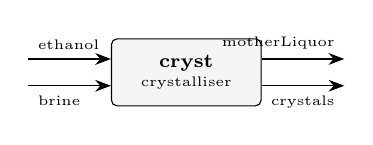
\begin{tikzpicture}[>={Stealth[length=2mm]}, every node/.style={font=\scriptsize}]
  \node[draw, rounded corners=2pt, align=center, minimum width=1.9cm, minimum height=0.85cm, fill=black!4] (cryst) at (0.0,-0.0) {\textbf{cryst}\\[-1pt]{\tiny crystalliser}};
  \draw[->] ($(cryst.west)+(-1.05,-0.17)$) -- ($(cryst.west)+(0,-0.17)$) node[at start, below, font=\tiny, anchor=north west] {brine};
  \draw[->] ($(cryst.west)+(-1.05,0.17)$) -- ($(cryst.west)+(0,0.17)$) node[at start, above, font=\tiny, anchor=south west] {ethanol};
  \draw[->] ($(cryst.east)+(0,-0.17)$) -- ($(cryst.east)+(1.05,-0.17)$) node[at end, below, font=\tiny, anchor=north east] {crystals};
  \draw[->] ($(cryst.east)+(0,0.17)$) -- ($(cryst.east)+(1.05,0.17)$) node[at end, above, font=\tiny, anchor=south east] {motherLiquor};
\end{tikzpicture}
\end{tutscheme}
\tutwhat{Antisolvent (drowning-out) crystallisation of NaCl: a SATURATED aqueous brine is mixed with ethanol; the eNRTL mixed-solvent term lowers the dielectric, raises gamma\_pm, and DROPS the saturation molality m\_sat -- so NaCl precipitates with NO cooling and NO evaporation. Saturation from the SAME ion-activity product Ksp anchored in pure water, solved with the mixed-solvent gamma\_pm.}
\begin{tutnarrative}
- Choupo -$\ast$--------------------------------$\ast$ | \textbackslash\{\}|/ C hemicals | Choupo: open-source, glass-box simulation | | \textbackslash\{\}\textbackslash\{\}|// H eat-transfer | Version: Choupo-dev | | \textbackslash\{\}\textbackslash\{\}\textbackslash\{\}|/// O perations | Website: https://choupo.org | | \textbackslash\{\}\textbackslash\{\}|// U nits | Licence: GPL-3.0-or-later | | \textbackslash\{\}|/ P roperties | Tutorial case file -- part of Choupo | | | O ptimization | |

\end{tutnarrative}
\begin{tutgolden}
\goldrow{stream}{brine}{F}{0.0277777777778}
\goldrow{stream}{crystals}{F}{0.00202035108762}
\goldrow{stream}{ethanol}{F}{0.0166666666667}
\goldrow{stream}{motherLiquor}{F}{0.0424240933568}
\goldrow{kpi}{cryst}{Ksp\_activity}{34.8439846653}
\goldrow{kpi}{cryst}{Q\_removed}{6559.87377671}
\goldrow{kpi}{cryst}{T\_op}{298.15}
\goldrow{kpi}{cryst}{antisolvent\_xfrac}{0.399920015997}
\goldrow{kpi}{cryst}{c\_sat}{0.0517444790334}
\goldrow{kpi}{cryst}{cakeLiquidFlow}{0.000329661969914}
\goldrow{kpi}{cryst}{cakeMoisture}{0.1}
\goldrow{kpi}{cryst}{cakeWetness\_pct}{9.09090909091}
\goldrow{kpi}{cryst}{crystal\_flow}{0.0988038720389}
\goldrow{kpi}{cryst}{crystal\_mol}{0.00169068911771}
\goldmore{8}
\end{tutgolden}

\clearpage
\tutentry{crystalliser07\_nacl\_antisolvent\_cooled}{tutorials/steady/crystallisation/crystalliser07\_nacl\_antisolvent\_cooled}
\begin{tutscheme}
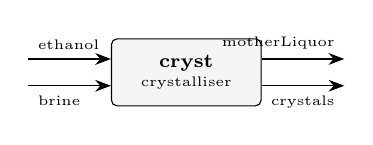
\begin{tikzpicture}[>={Stealth[length=2mm]}, every node/.style={font=\scriptsize}]
  \node[draw, rounded corners=2pt, align=center, minimum width=1.9cm, minimum height=0.85cm, fill=black!4] (cryst) at (0.0,-0.0) {\textbf{cryst}\\[-1pt]{\tiny crystalliser}};
  \draw[->] ($(cryst.west)+(-1.05,-0.17)$) -- ($(cryst.west)+(0,-0.17)$) node[at start, below, font=\tiny, anchor=north west] {brine};
  \draw[->] ($(cryst.west)+(-1.05,0.17)$) -- ($(cryst.west)+(0,0.17)$) node[at start, above, font=\tiny, anchor=south west] {ethanol};
  \draw[->] ($(cryst.east)+(0,-0.17)$) -- ($(cryst.east)+(1.05,-0.17)$) node[at end, below, font=\tiny, anchor=north east] {crystals};
  \draw[->] ($(cryst.east)+(0,0.17)$) -- ($(cryst.east)+(1.05,0.17)$) node[at end, above, font=\tiny, anchor=south east] {motherLiquor};
\end{tikzpicture}
\end{tutscheme}
\tutwhat{Antisolvent + COOLING crystallisation of NaCl: the same drowning-out brine + ethanol as crystalliser06, but the crystalliser is COOLED to 5 C. The eNRTL is now temperature-dependent (tau(T)=tau\_25$\ast$298.15/T, A\_DH(T) via eps\_w(T)/rho\_w(T), Born at T) and Ksp(T) shifts by van't Hoff with NaCl's enthalpy of solution -- so cooling adds to the antisolvent's effect (yield 61\% $\to$ 70\%). Exercises the T-dependent electrolyte path.}
\begin{tutnarrative}
- Choupo -$\ast$--------------------------------$\ast$ | \textbackslash\{\}|/ C hemicals | Choupo: open-source, glass-box simulation | | \textbackslash\{\}\textbackslash\{\}|// H eat-transfer | Version: Choupo-dev | | \textbackslash\{\}\textbackslash\{\}\textbackslash\{\}|/// O perations | Website: https://choupo.org | | \textbackslash\{\}\textbackslash\{\}|// U nits | Licence: GPL-3.0-or-later | | \textbackslash\{\}|/ P roperties | Tutorial case file -- part of Choupo | | | O ptimization | |

\end{tutnarrative}
\begin{tutgolden}
\goldrow{stream}{brine}{F}{0.0277777777778}
\goldrow{stream}{crystals}{F}{0.00231987381407}
\goldrow{stream}{ethanol}{F}{0.0166666666667}
\goldrow{stream}{motherLiquor}{F}{0.0421245706304}
\goldrow{kpi}{cryst}{Ksp\_activity}{31.135192385}
\goldrow{kpi}{cryst}{Q\_removed}{82721.44242}
\goldrow{kpi}{cryst}{T\_op}{278.15}
\goldrow{kpi}{cryst}{antisolvent\_xfrac}{0.399920015997}
\goldrow{kpi}{cryst}{c\_sat}{0.0398065230351}
\goldrow{kpi}{cryst}{cakeLiquidFlow}{0.000380305320939}
\goldrow{kpi}{cryst}{cakeMoisture}{0.1}
\goldrow{kpi}{cryst}{cakeWetness\_pct}{9.09090909091}
\goldrow{kpi}{cryst}{crystal\_flow}{0.113348382739}
\goldrow{kpi}{cryst}{crystal\_mol}{0.00193956849313}
\goldmore{8}
\end{tutgolden}

\clearpage
\tutentry{crystalliser08\_nacl\_antisolvent\_msmpr}{tutorials/steady/crystallisation/crystalliser08\_nacl\_antisolvent\_msmpr}
\begin{tutscheme}
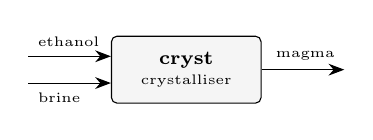
\begin{tikzpicture}[>={Stealth[length=2mm]}, every node/.style={font=\scriptsize}]
  \node[draw, rounded corners=2pt, align=center, minimum width=1.9cm, minimum height=0.85cm, fill=black!4] (cryst) at (0.0,-0.0) {\textbf{cryst}\\[-1pt]{\tiny crystalliser}};
  \draw[->] ($(cryst.west)+(-1.05,-0.17)$) -- ($(cryst.west)+(0,-0.17)$) node[at start, below, font=\tiny, anchor=north west] {brine};
  \draw[->] ($(cryst.west)+(-1.05,0.17)$) -- ($(cryst.west)+(0,0.17)$) node[at start, above, font=\tiny, anchor=south west] {ethanol};
  \draw[->] ($(cryst.east)+(0,0.00)$) -- ($(cryst.east)+(1.05,0.00)$) node[at end, above, font=\tiny, anchor=south east] {magma};
\end{tikzpicture}
\end{tutscheme}
\tutwhat{Continuous MSMPR antisolvent crystallisation of NaCl: a saturated brine + ethanol fed to a well-mixed vessel (residence time tau = V/Q). The eNRTL antisolvent supersaturation S = c/c\_sat(eNRTL) drives nucleation + growth; the method of moments closes the population balance and returns the CRYSTAL-SIZE DISTRIBUTION n(L) (mean size, CV) -- what the equilibrium model cannot give.}
\begin{tutnarrative}
- Choupo -$\ast$--------------------------------$\ast$ | \textbackslash\{\}|/ C hemicals | Choupo: open-source, glass-box simulation | | \textbackslash\{\}\textbackslash\{\}|// H eat-transfer | Version: Choupo-dev | | \textbackslash\{\}\textbackslash\{\}\textbackslash\{\}|/// O perations | Website: https://choupo.org | | \textbackslash\{\}\textbackslash\{\}|// U nits | Licence: GPL-3.0-or-later | | \textbackslash\{\}|/ P roperties | Tutorial case file -- part of Choupo | | | O ptimization | |

\end{tutnarrative}
\begin{tutgolden}
\goldrow{stream}{brine}{F}{0.0277777777778}
\goldrow{stream}{ethanol}{F}{0.0166666666667}
\goldrow{stream}{magma}{F}{0.0444444444444}
\goldrow{kpi}{cryst}{CV}{1}
\goldrow{kpi}{cryst}{L\_dominant}{2.02534396647e-05}
\goldrow{kpi}{cryst}{L\_meanMass}{2.70045862196e-05}
\goldrow{kpi}{cryst}{L\_meanNumber}{6.75114655489e-06}
\goldrow{kpi}{cryst}{Q\_kW}{-6.1566687571}
\goldrow{kpi}{cryst}{Q\_removed}{6156.6687571}
\goldrow{kpi}{cryst}{T\_op}{298.15}
\goldrow{kpi}{cryst}{c\_sat}{0.0517444790334}
\goldrow{kpi}{cryst}{crystal\_flow}{0.092730856228}
\goldrow{kpi}{cryst}{crystal\_mol}{0.00158677029822}
\goldrow{kpi}{cryst}{growthRate}{1.92664299147e-09}
\goldmore{12}
\end{tutgolden}

\clearpage
\tutentry{crystalliser09\_KHT\_KCl\_series}{tutorials/steady/crystallisation/crystalliser09\_KHT\_KCl\_series}
\begin{tutscheme}
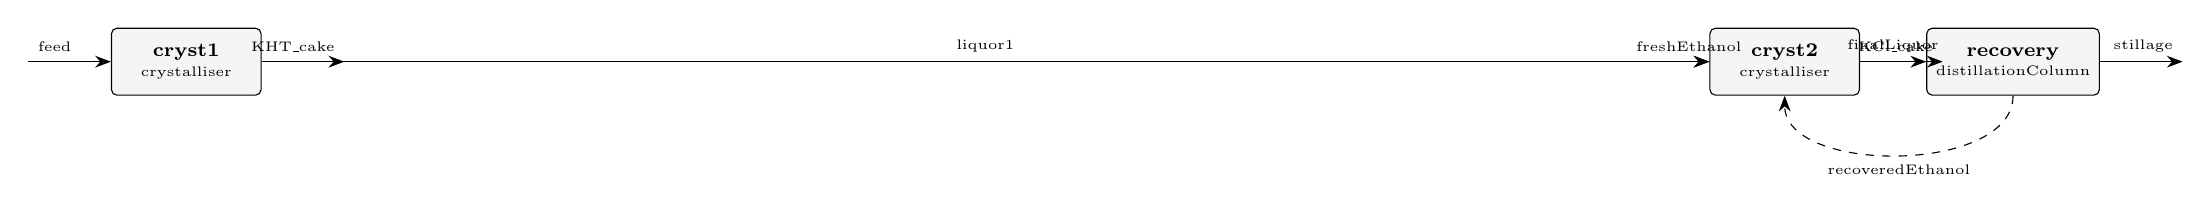
\begin{tikzpicture}[>={Stealth[length=2mm]}, every node/.style={font=\scriptsize}]
  \node[draw, rounded corners=2pt, align=center, minimum width=1.9cm, minimum height=0.85cm, fill=black!4] (cryst1) at (0.0,-0.0) {\textbf{cryst1}\\[-1pt]{\tiny crystalliser}};
  \node[draw, rounded corners=2pt, align=center, minimum width=1.9cm, minimum height=0.85cm, fill=black!4] (cryst2) at (20.3,-0.0) {\textbf{cryst2}\\[-1pt]{\tiny crystalliser}};
  \node[draw, rounded corners=2pt, align=center, minimum width=1.9cm, minimum height=0.85cm, fill=black!4] (recovery) at (23.2,-0.0) {\textbf{recovery}\\[-1pt]{\tiny distillationColumn}};
  \draw[->] ($(cryst1.west)+(-1.05,0.00)$) -- ($(cryst1.west)+(0,0.00)$) node[at start, above, font=\tiny, anchor=south west] {feed};
  \draw[->] (cryst1) -- (cryst2) node[midway, above, font=\tiny] {liquor1};
  \draw[->] ($(cryst2.west)+(-1.05,0.00)$) -- ($(cryst2.west)+(0,0.00)$) node[at start, above, font=\tiny, anchor=south west] {freshEthanol};
  \draw[->, dashed] (recovery.south) .. controls +(0,-1.0) and +(0,-1.0) .. (cryst2.south) node[midway, below, font=\tiny] {recoveredEthanol};
  \draw[->] (cryst2) -- (recovery) node[midway, above, font=\tiny] {finalLiquor};
  \draw[->] ($(cryst1.east)+(0,0.00)$) -- ($(cryst1.east)+(1.05,0.00)$) node[at end, above, font=\tiny, anchor=south east] {KHT\_cake};
  \draw[->] ($(cryst2.east)+(0,0.00)$) -- ($(cryst2.east)+(1.05,0.00)$) node[at end, above, font=\tiny, anchor=south east] {KCl\_cake};
  \draw[->] ($(recovery.east)+(0,0.00)$) -- ($(recovery.east)+(1.05,0.00)$) node[at end, above, font=\tiny, anchor=south east] {stillage};
\end{tikzpicture}
\end{tutscheme}
\tutwhat{Two crystallisers in series separating KCl from potassium bitartrate (KHT, cream of tartar) by manipulating T and adding ethanol. CRYST1 COOLS the hot feed to 5 C $\to$ KHT (sparingly soluble, steep solubility curve) crystallises while KCl stays dissolved. CRYST2 doses ETHANOL into the KCl-rich mother liquor $\to$ KCl drops out by drowning-out (eNRTL mixed-solvent). Two salts, two saturation routes (curve vs ion-activity), one package -- a stress test of the property system.}
\begin{tutnarrative}
- Choupo -$\ast$--------------------------------$\ast$ | \textbackslash\{\}|/ C hemicals | Choupo: open-source, glass-box simulation | | \textbackslash\{\}\textbackslash\{\}|// H eat-transfer | Version: Choupo-dev | | \textbackslash\{\}\textbackslash\{\}\textbackslash\{\}|/// O perations | Website: https://choupo.org | | \textbackslash\{\}\textbackslash\{\}|// U nits | Licence: GPL-3.0-or-later | | \textbackslash\{\}|/ P roperties | Tutorial case file -- part of Choupo | | | O ptimization | |

\end{tutnarrative}
\begin{tutgolden}
\goldrow{stream}{KCl\_cake}{F}{0.00138859586739}
\goldrow{stream}{KHT\_cake}{F}{5.38404641059e-05}
\goldrow{stream}{feed}{F}{0.0277777777792}
\goldrow{stream}{finalLiquor}{F}{0.0541131192255}
\goldrow{stream}{freshEthanol}{F}{0.00416666666667}
\goldrow{stream}{liquor1}{F}{0.0277239373151}
\goldrow{stream}{recoveredEthanol}{F}{0.0236111111111}
\goldrow{stream}{stillage}{F}{0.0305020081144}
\goldrow{kpi}{cryst1}{Q\_kW}{-93.1162690166}
\goldrow{kpi}{cryst1}{Q\_removed}{93116.2690166}
\goldrow{kpi}{cryst1}{T\_op}{278.15}
\goldrow{kpi}{cryst1}{c\_sat}{0.0034013435}
\goldrow{kpi}{cryst1}{cakeLiquidFlow}{2.54671494088e-05}
\goldrow{kpi}{cryst1}{cakeMoisture}{0.1}
\goldmore{47}
\end{tutgolden}

\clearpage
\tutentry{crystalliser10\_naoh\_antisolvent}{tutorials/steady/crystallisation/crystalliser10\_naoh\_antisolvent}
\begin{tutscheme}
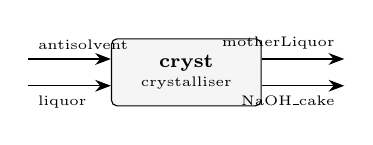
\begin{tikzpicture}[>={Stealth[length=2mm]}, every node/.style={font=\scriptsize}]
  \node[draw, rounded corners=2pt, align=center, minimum width=1.9cm, minimum height=0.85cm, fill=black!4] (cryst) at (0.0,-0.0) {\textbf{cryst}\\[-1pt]{\tiny crystalliser}};
  \draw[->] ($(cryst.west)+(-1.05,-0.17)$) -- ($(cryst.west)+(0,-0.17)$) node[at start, below, font=\tiny, anchor=north west] {liquor};
  \draw[->] ($(cryst.west)+(-1.05,0.17)$) -- ($(cryst.west)+(0,0.17)$) node[at start, above, font=\tiny, anchor=south west] {antisolvent};
  \draw[->] ($(cryst.east)+(0,-0.17)$) -- ($(cryst.east)+(1.05,-0.17)$) node[at end, below, font=\tiny, anchor=north east] {NaOH\_cake};
  \draw[->] ($(cryst.east)+(0,0.17)$) -- ($(cryst.east)+(1.05,0.17)$) node[at end, above, font=\tiny, anchor=south east] {motherLiquor};
\end{tikzpicture}
\end{tutscheme}
\tutwhat{NaOH antisolvent crystallisation (water + ethanol, eNRTL drowning-out) -- the acceptance-case core}
\begin{tutnarrative}
- Choupo -$\ast$--------------------------------$\ast$ | \textbackslash\{\}|/ C hemicals | Choupo: open-source, glass-box simulation | | \textbackslash\{\}\textbackslash\{\}|// H eat-transfer | Version: Choupo-dev | | \textbackslash\{\}\textbackslash\{\}\textbackslash\{\}|/// O perations | Website: https://choupo.org | | \textbackslash\{\}\textbackslash\{\}|// U nits | Licence: GPL-3.0-or-later | | \textbackslash\{\}|/ P roperties | Tutorial case file -- part of Choupo | | | O ptimization | |

\end{tutnarrative}
\begin{tutgolden}
\goldrow{stream}{NaOH\_cake}{F}{0.00183771747926}
\goldrow{stream}{antisolvent}{F}{0.00833333333333}
\goldrow{stream}{liquor}{F}{0.0138888888889}
\goldrow{stream}{motherLiquor}{F}{0.020384504743}
\goldrow{kpi}{cryst}{Ksp\_activity}{7365.8380048}
\goldrow{kpi}{cryst}{Q\_kW}{72.7276039114}
\goldrow{kpi}{cryst}{Q\_removed}{-72727.6039114}
\goldrow{kpi}{cryst}{T\_op}{298.15}
\goldrow{kpi}{cryst}{antisolvent\_xfrac}{0.461538461538}
\goldrow{kpi}{cryst}{c\_sat}{0.181200024556}
\goldrow{kpi}{cryst}{cakeLiquidFlow}{0.000203756483719}
\goldrow{kpi}{cryst}{cakeMoisture}{0.1}
\goldrow{kpi}{cryst}{cakeWetness\_pct}{9.09090909091}
\goldrow{kpi}{cryst}{crystal\_flow}{0.0653535379386}
\goldmore{9}
\end{tutgolden}

\clearpage
\tutentry{crystalliser11\_kcl\_antisolvent\_ethanol}{tutorials/steady/crystallisation/crystalliser11\_kcl\_antisolvent\_ethanol}
\begin{tutscheme}
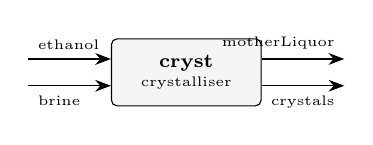
\begin{tikzpicture}[>={Stealth[length=2mm]}, every node/.style={font=\scriptsize}]
  \node[draw, rounded corners=2pt, align=center, minimum width=1.9cm, minimum height=0.85cm, fill=black!4] (cryst) at (0.0,-0.0) {\textbf{cryst}\\[-1pt]{\tiny crystalliser}};
  \draw[->] ($(cryst.west)+(-1.05,-0.17)$) -- ($(cryst.west)+(0,-0.17)$) node[at start, below, font=\tiny, anchor=north west] {brine};
  \draw[->] ($(cryst.west)+(-1.05,0.17)$) -- ($(cryst.west)+(0,0.17)$) node[at start, above, font=\tiny, anchor=south west] {ethanol};
  \draw[->] ($(cryst.east)+(0,-0.17)$) -- ($(cryst.east)+(1.05,-0.17)$) node[at end, below, font=\tiny, anchor=north east] {crystals};
  \draw[->] ($(cryst.east)+(0,0.17)$) -- ($(cryst.east)+(1.05,0.17)$) node[at end, above, font=\tiny, anchor=south east] {motherLiquor};
\end{tikzpicture}
\end{tutscheme}
\tutwhat{Antisolvent (drowning-out) crystallisation of KCl: a SATURATED aqueous KCl brine (4.76 mol/kg) is mixed with ethanol; the eNRTL mixed-solvent term lowers the dielectric, raises gamma\_pm, and DROPS the saturation molality -- so KCl precipitates with NO cooling and NO evaporation. Saturation is the SAME ion-activity product Ksp anchored in pure water, solved with the mixed-solvent gamma\_pm at the feed's salt-free ethanol fraction. KCl-water-ethanol experimental reference: Lopes, Farelo \& Ferra, J. Solution Chem. 28 (1999) 117.}
\begin{tutnarrative}
- Choupo -$\ast$--------------------------------$\ast$ | \textbackslash\{\}|/ C hemicals | Choupo: open-source, glass-box simulation | | \textbackslash\{\}\textbackslash\{\}|// H eat-transfer | Version: Choupo-dev | | \textbackslash\{\}\textbackslash\{\}\textbackslash\{\}|/// O perations | Website: https://choupo.org | | \textbackslash\{\}\textbackslash\{\}|// U nits | Licence: GPL-3.0-or-later | | \textbackslash\{\}|/ P roperties | Tutorial case file -- part of Choupo | | | O ptimization | |

\end{tutnarrative}
\tutreadme{The KCl counterpart of crystalliser06 (NaCl): a saturated aqueous KCl brine is mixed with ethanol, whose low dielectric collapses the KCl solubility, so KCl crystallises with no cooling and no evaporation. KCl is the salt the catalogue's KCl.dat names as $\ast$"recovered by ANTISOLVENT (drowning-out with ethanol)"$\ast$ --- this case realises it.}
\tutreadme{Ethanol's relative permittivity (24.3) is far below water's (78.5). Dosing it lowers the mixed-solvent dielectric, which raises the mean ionic activity coefficient $\gamma$$\pm$ (eNRTL mixed-solvent + Born term), so the saturation molality collapses. The saturation is the same ion-activity product Ksp = ($\gamma$$\pm$ $\cdot$ m\_sat)$^2$ anchored in pure water, re-solved with the mixed-solvent $\gamma$$\pm$ at the feed's salt-free ethanol fraction --- the physics the aqueous Pitzer model cannot reach (the reason eNRTL exists).}
\tutreadme{100 kmol/h saturated brine (x\_water 0.921, x\_KCl 0.079 = 4.76 mol/kg) + 60 kmol/h ethanol $\to$ salt-free x\_ethanol $\approx$ 0.39:}
\tutreadme{The KCl--water--ethanol activity behaviour modelled here is measured in A. Lopes, F. Farelo \& M. I. A. Ferra, "Activity Coefficients of Potassium Chloride in Water--Ethanol Mixtures", $\ast$J. Solution Chem.$\ast$ 28 (1999) 117 --- mean activity coefficients of KCl by emf in 5--20 \% w/w ethanol, 25--45 $^\circ$C. That $\gamma$$\pm$ rise with ethanol content is exactly the driver of the drowning-out captured above.}
\tutreadme{- The eNRTL $\tau$ for K--Cl is the illustrative 1:1-alkali-chloride proxy (= Chen \& Evans water--NaCl), so the numbers are qualitative. The Farelo data is the path to a quantitative refit of the KCl--water--ethanol interaction (the paper reports Pitzer $\beta$$^0$/$\beta$$^1$/C? per solvent composition). - The mass / yield is the reliable output. The crystalliser's heat term carries the shared electrolyte-enthalpy caveat (a dissolved salt's formation datum lives in its ions, so the stream enthalpy falls back to the sensible datum and is announced) --- identical to crystalliser06.}
\begin{tutgolden}
\goldrow{stream}{brine}{F}{0.0277777777778}
\goldrow{stream}{crystals}{F}{0.0021050886953}
\goldrow{stream}{ethanol}{F}{0.0166666666667}
\goldrow{stream}{motherLiquor}{F}{0.0423393557491}
\goldrow{kpi}{cryst}{Ksp\_activity}{7.69319557877}
\goldrow{kpi}{cryst}{Q\_kW}{-28.9281906957}
\goldrow{kpi}{cryst}{Q\_removed}{28928.1906957}
\goldrow{kpi}{cryst}{T\_op}{298.15}
\goldrow{kpi}{cryst}{antisolvent\_xfrac}{0.394477317554}
\goldrow{kpi}{cryst}{c\_sat}{0.0311001943033}
\goldrow{kpi}{cryst}{cakeLiquidFlow}{0.000423217143227}
\goldrow{kpi}{cryst}{cakeMoisture}{0.1}
\goldrow{kpi}{cryst}{cakeWetness\_pct}{9.09090909091}
\goldrow{kpi}{cryst}{crystal\_flow}{0.125385206079}
\goldmore{9}
\end{tutgolden}

\clearpage
\tutentry{crystalliser12\_nacl\_pitzer\_antisolvent}{tutorials/steady/crystallisation/crystalliser12\_nacl\_pitzer\_antisolvent}
\begin{tutscheme}
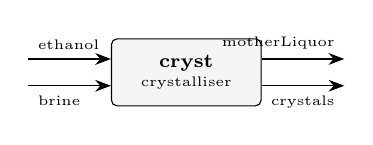
\begin{tikzpicture}[>={Stealth[length=2mm]}, every node/.style={font=\scriptsize}]
  \node[draw, rounded corners=2pt, align=center, minimum width=1.9cm, minimum height=0.85cm, fill=black!4] (cryst) at (0.0,-0.0) {\textbf{cryst}\\[-1pt]{\tiny crystalliser}};
  \draw[->] ($(cryst.west)+(-1.05,-0.17)$) -- ($(cryst.west)+(0,-0.17)$) node[at start, below, font=\tiny, anchor=north west] {brine};
  \draw[->] ($(cryst.west)+(-1.05,0.17)$) -- ($(cryst.west)+(0,0.17)$) node[at start, above, font=\tiny, anchor=south west] {ethanol};
  \draw[->] ($(cryst.east)+(0,-0.17)$) -- ($(cryst.east)+(1.05,-0.17)$) node[at end, below, font=\tiny, anchor=north east] {crystals};
  \draw[->] ($(cryst.east)+(0,0.17)$) -- ($(cryst.east)+(1.05,0.17)$) node[at end, above, font=\tiny, anchor=south east] {motherLiquor};
\end{tikzpicture}
\end{tutscheme}
\tutwhat{Pitzer + antisolvent: the calorimetric L\_phi fit is AQUEOUS, so a mixed solvent drops it -- and the duty basis says so}
\begin{tutnarrative}
- Choupo -$\ast$--------------------------------$\ast$ | \textbackslash\{\}|/ C hemicals | Choupo: open-source, glass-box simulation | | \textbackslash\{\}\textbackslash\{\}|// H eat-transfer | Version: Choupo-dev | | \textbackslash\{\}\textbackslash\{\}\textbackslash\{\}|/// O perations | Website: https://choupo.org | | \textbackslash\{\}\textbackslash\{\}|// U nits | Licence: GPL-3.0-or-later | | \textbackslash\{\}|/ P roperties | Tutorial case file -- part of Choupo | | | O ptimization | |

\end{tutnarrative}
\begin{tutgolden}
\goldrow{stream}{brine}{F}{0.0277777777778}
\goldrow{stream}{crystals}{F}{0}
\goldrow{stream}{ethanol}{F}{0.0166666666667}
\goldrow{stream}{motherLiquor}{F}{0.0444444444444}
\goldrow{kpi}{cryst}{Ksp\_activity}{38.4846213082}
\goldrow{kpi}{cryst}{Q\_kW}{-0}
\goldrow{kpi}{cryst}{Q\_removed}{0}
\goldrow{kpi}{cryst}{T\_op}{298.15}
\goldrow{kpi}{cryst}{antisolvent\_xfrac}{0.399920015997}
\goldrow{kpi}{cryst}{c\_sat}{0.35905536}
\goldrow{kpi}{cryst}{cakeLiquidFlow}{0}
\goldrow{kpi}{cryst}{cakeMoisture}{0.1}
\goldrow{kpi}{cryst}{cakeWetness\_pct}{0}
\goldrow{kpi}{cryst}{crystal\_flow}{0}
\goldmore{9}
\end{tutgolden}

\clearpage
\tutentry{overlay02\_nacl\_calorimetric}{tutorials/steady/crystallisation/overlay02\_nacl\_calorimetric}
\tutwhat{NaCl crystalliser: saturation from the PITZER ion activity (Ksp = (gamma\_pm$\ast$m\_sat)\textasciicircum{}2). Feed is a SUPERSATURATED brine (post-evaporation, \textasciitilde{}7.6 mol/kg); the unit drops it to saturation (6.144 mol/kg) and crystallises the excess.}
\begin{tutnarrative}
- Choupo -$\ast$--------------------------------$\ast$ | \textbackslash\{\}|/ C hemicals | Choupo: open-source, glass-box simulation | | \textbackslash\{\}\textbackslash\{\}|// H eat-transfer | Version: Choupo-dev | | \textbackslash\{\}\textbackslash\{\}\textbackslash\{\}|/// O perations | Website: https://choupo.org | | \textbackslash\{\}\textbackslash\{\}|// U nits | Licence: GPL-3.0-or-later | | \textbackslash\{\}|/ P roperties | Tutorial case file -- part of Choupo | | | O ptimization | |

\end{tutnarrative}
\tutreadme{A NaCl crystalliser (cloned from crystalliser05) whose case-local constant/components/NaCl.dat declares overlayOf NaCl; and recalibrates ONLY solidPhases.halite.calorimetric.dissolutionEnthalpy (3880 $\to$ 5880 J/mol).}
\tutreadme{The ThermoPackageBuilder deep-merges this delta over the standard record, so the crystalliser duty reflects it: Q\_removed = 3690.997 W here vs 2435.556 in crystalliser05 (ratio 1.515 = 5880/3880). Every other KPI (Ksp\_activity, m\_sat, c\_sat, crystal\_mol, gamma) is byte-identical to crystalliser05 -- logK25, dH, the dissolution reaction and the crystal block all still come from the standard.}
\tutreadme{This is the second half of the roadmap Phase A acceptance test: the SINGLE unified reader applies the overlay at ALL three component-loading sites (SpeciationSolver, Database, ThermoPackageBuilder), not just the SI path.}
\begin{tutgolden}
\goldrow{stream}{feed}{F}{0.0277777777778}
\goldrow{stream}{magma}{F}{0.0277777777778}
\goldrow{kpi}{cryst}{Ksp\_activity}{38.4846213082}
\goldrow{kpi}{cryst}{Q\_kW}{-2.50670156624}
\goldrow{kpi}{cryst}{Q\_removed}{2506.70156624}
\goldrow{kpi}{cryst}{T\_op}{298.15}
\goldrow{kpi}{cryst}{c\_sat}{0.35905536}
\goldrow{kpi}{cryst}{crystal\_flow}{0.036683987968}
\goldrow{kpi}{cryst}{crystal\_mol}{0.000627720533333}
\goldrow{kpi}{cryst}{gamma\_pm\_sat}{1.00970010562}
\goldrow{kpi}{cryst}{liquorFlow}{0.0271500572444}
\goldrow{kpi}{cryst}{m\_sat}{6.144}
\goldrow{kpi}{cryst}{solute\_dissolved}{0.158116012032}
\goldrow{kpi}{cryst}{solute\_in}{0.1948}
\goldmore{1}
\end{tutgolden}

\subsection{distillation}
\grouptheory{distillation}
\clearpage
\tutentry{acetone06\_luyben\_column\_C1}{tutorials/steady/distillation/acetone06\_luyben\_column\_C1}
\begin{tutscheme}
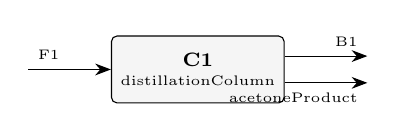
\begin{tikzpicture}[>={Stealth[length=2mm]}, every node/.style={font=\scriptsize}]
  \node[draw, rounded corners=2pt, align=center, minimum width=1.9cm, minimum height=0.85cm, fill=black!4] (C1) at (0.0,-0.0) {\textbf{C1}\\[-1pt]{\tiny distillationColumn}};
  \draw[->] ($(C1.west)+(-1.05,0.00)$) -- ($(C1.west)+(0,0.00)$) node[at start, above, font=\tiny, anchor=south west] {F1};
  \draw[->] ($(C1.east)+(0,-0.17)$) -- ($(C1.east)+(1.05,-0.17)$) node[at end, below, font=\tiny, anchor=north east] {acetoneProduct};
  \draw[->] ($(C1.east)+(0,0.17)$) -- ($(C1.east)+(1.05,0.17)$) node[at end, above, font=\tiny, anchor=south east] {B1};
\end{tikzpicture}
\end{tutscheme}
\tutwhat{Luyben's acetone column C1 on predictive UNIFAC: the test of a prediction written before the column was built}
\begin{tutnarrative}
THE COLUMN THAT TESTS A PREDICTION WRITTEN BEFORE IT EXISTED.

W. L. Luyben, Ind. Eng. Chem. Res. 50 (2011) 1206-1218, DOI 10.1021/ie901923a. Column C1 of his Figure 1: 66 stages, feed on stage 54, reflux ratio 2.78, distillate 32.25 kmol/h, 1 atm. It takes the combined flash liquid plus absorber bottoms (his F1) and is asked to make the ACETONE PRODUCT at 99.9 mol \%.

THE PREDICTION, quoted from the sibling props case rather than reinvented. `props/compare/acetone04\_acetone\_water\_vle` measured the acetone/water VLE this column rests on BEFORE any column was built, and found that predictive UNIFAC puts a minimum-boiling azeotrope at x\_acetone \textasciitilde{} 0.978 where Luyben's UNIQUAC has only a pinch. It is a tiny feature -- 0.044 K deep, |y - x| never above 7.7e-4 -- and acetone04 recorded, in advance and in writing:

"A column C1 built on this thermodynamics should be expected to asymptote near 97.9 \% and fail his spec -- and if it had been built before this was measured, the column would have been blamed for a defect that lives in the activity model."

So THIS case has a pass/fail criterion that is not its own golden: either the distillate stalls near the predicted ceiling, or the prediction was wrong. Both outcomes are results. Neither is a reason to touch the thermodynamics.

THE FEED IS LUYBEN'S OWN F1, not this project's upstream answer. acetone03 computes a flash liquid and acetone05 an absorber bottoms, and their sum is what physically feeds C1 -- but wiring them in would test the column and two upstream units at once, and acetone05 already reports that it recovers a sixth of what the paper does. Feeding the PUBLISHED stream isolates the column: whatever it gets wrong here is the column and its thermodynamics. The composition in 0/F1 is his mole fractions times his 72.85 kmol/h.

WHAT IS NOT LUYBEN'S, and why each choice is the honest one:

UNIQUAC vs UNIFAC. He runs UNIQUAC; Choupo ships no fitted pair for any of these binaries and inventing one would convert unsourced into falsely sourced. Predictive UNIFAC is what is available, and acetone04 measured what it costs on the binary that decides this column.

The rigorous MESH (`model simultaneous`). Wang-Henke is the corpus default and is documented as unstable through an azeotrope, which is precisely the feature under test here. Choosing the method that CAN resolve the feature is not tuning; choosing the one that cannot would have hidden it.

Isopropanol's liquid heat capacity is Rowlinson-Bondi off the same Joback fragmentation as the rest of its record. Its measured accuracy on hydrogen-bonding molecules is 30-70 \%, stated in the record itself. It is 5 mol \% of the feed and it moves the DUTIES, not the split.

THIS COLUMN IS MODELLED DOWNSTREAM OF LUYBEN'S VENT, so it carries no hydrogen. His C1 has a partial condenser with a vent; Choupo's column has a total condenser and no vapour distillate. Both facts are stated before the reason, because the reason has to be argued rather than asserted:

- his vent is 0.0465 kmol/h at H2 0.2798, i.e. 0.0130 kmol/h of hydrogen, against the 0.0146 kmol/h that F1 carries. The vent removes essentially ALL of it. A column model with no vent and a total condenser therefore represents the column AFTER the vent, which is a statement about WHICH UNIT is being modelled -- not an approximation to the physics of the one that is.

- what that costs is quantified rather than hidden: the same vent carries 0.0335 kmol/h of ACETONE (his own figure), 0.10 \% of the product. Not modelling the vent therefore FLATTERS this column's acetone recovery by that much, and the comparison below must be read knowing it.

IT WAS RUN THE OTHER WAY FIRST, and the run is the reason this paragraph exists rather than a preference. With H2 in the feed the MESH converged (16 Newton iterations, ||F|| 2.4e-11) to the SAME distillate -- x\_acetone 0.9722 -- and then the energy report REFUSED: hydrogen has no liquid heat capacity, because at 330 K it has no liquid. The refusal is right, and it is the honest form of the modelling error: a total condenser was silently asking a permanent gas to leave as a liquid. See this case's CLAUDE.md.

\end{tutnarrative}
\begin{tutgolden}
\goldrow{stream}{B1}{F}{0.0112717083333}
\goldrow{stream}{F1}{F}{0.0202300416667}
\goldrow{stream}{acetoneProduct}{F}{0.00895833333333}
\goldrow{kpi}{C1}{B}{0.0112717083333}
\goldrow{kpi}{C1}{D}{0.00895833333333}
\goldrow{kpi}{C1}{Q\_condenser\_kW}{-997.746586798}
\goldrow{kpi}{C1}{Q\_reboiler\_kW}{1030.49217736}
\goldrow{kpi}{C1}{R}{2.78}
\goldrow{kpi}{C1}{T\_bottom}{353.606283382}
\goldrow{kpi}{C1}{T\_top}{329.375698025}
\goldrow{kpi}{C1}{feedStage}{54}
\goldrow{kpi}{C1}{nFeeds}{1}
\goldrow{kpi}{C1}{nSideDraws}{0}
\goldrow{kpi}{C1}{nStages}{66}
\goldmore{14}
\end{tutgolden}

\clearpage
\tutentry{acetone07\_luyben\_column\_C2}{tutorials/steady/distillation/acetone07\_luyben\_column\_C2}
\begin{tutscheme}
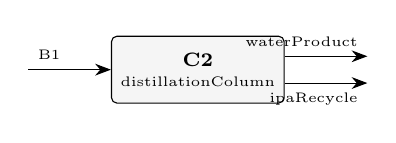
\begin{tikzpicture}[>={Stealth[length=2mm]}, every node/.style={font=\scriptsize}]
  \node[draw, rounded corners=2pt, align=center, minimum width=1.9cm, minimum height=0.85cm, fill=black!4] (C2) at (0.0,-0.0) {\textbf{C2}\\[-1pt]{\tiny distillationColumn}};
  \draw[->] ($(C2.west)+(-1.05,0.00)$) -- ($(C2.west)+(0,0.00)$) node[at start, above, font=\tiny, anchor=south west] {B1};
  \draw[->] ($(C2.east)+(0,-0.17)$) -- ($(C2.east)+(1.05,-0.17)$) node[at end, below, font=\tiny, anchor=north east] {ipaRecycle};
  \draw[->] ($(C2.east)+(0,0.17)$) -- ($(C2.east)+(1.05,0.17)$) node[at end, above, font=\tiny, anchor=south east] {waterProduct};
\end{tikzpicture}
\end{tutscheme}
\tutwhat{Luyben's water column C2: the IPA recycle meets the azeotrope acetone01 measured}
\begin{tutnarrative}
THE SECOND COLUMN, AND THE SECOND PREDICTION WRITTEN BEFORE IT.

W. L. Luyben, Ind. Eng. Chem. Res. 50 (2011) 1206-1218, DOI 10.1021/ie901923a. Column C2 of his Figure 1: 19 stages, feed on stage 16, reflux ratio 0.849, 1 atm. It takes C1's bottoms and makes the plant's WATER PRODUCT at the bottom (34.67 kmol/h, 99.9 mol \% water) while sending the unconverted isopropanol back overhead as the RECYCLE (5.88 kmol/h at x\_IPA 0.6500).

THE PREDICTION, quoted from acetone01 rather than reinvented, and committed to the repository BEFORE this case was written:

"C2's overhead should cap at roughly x\_IPA 0.59 and cannot reach his 0.650. The gap is 0.06 in mole fraction, about 9 \% relative, and it is a HARD ceiling rather than a shortfall in stages or reflux."

The reason is one measured number: acetone01 puts the UNIFAC IPA/water azeotrope at x\_IPA 0.5901 against Luyben's UNIQUAC value of 0.6732. A column cannot distil past a minimum-boiling azeotrope from below.

AND THE DIRECTION OF THIS ERROR IS THE OPPOSITE OF C1's, which is the part worth carrying away. C1's azeotrope is a UNIFAC INVENTION -- Luyben's model has none in acetone/water -- so it costs purity the paper does not lose. Here the azeotrope is REAL in both models and UNIFAC merely puts it in the wrong place. One failure is a spurious feature; the other is a misplaced real one. They are not the same defect and should not be reported as one.

THE FEED IS LUYBEN'S PUBLISHED B1, not acetone06's answer -- the same choice and the same reason as in C1: it isolates the column. His B1 is 40.56 kmol/h at 370 K, A 0.0001 / IPA 0.0951 / W 0.9048. The CLOSED flowsheet (acetone08) is where the two columns finally see each other's real streams, and the difference between this case and that one is exactly the propagation the plant exists to show.

THE DISTILLATE RATE IS HIS, 5.88 kmol/h, and that matters here in a way it did not in C1. Fixing the rate means the column must send that much material overhead whatever its composition can be -- so if the ceiling binds, it shows up as a WETTER recycle at the same flow, not as a smaller one. That is the honest way to pose it: the plant's IPA inventory has to go somewhere, and the question is what quality it comes back at.

\end{tutnarrative}
\begin{tutgolden}
\goldrow{stream}{B1}{F}{0.0112666944444}
\goldrow{stream}{ipaRecycle}{F}{0.00163333333333}
\goldrow{stream}{waterProduct}{F}{0.00963336111111}
\goldrow{kpi}{C2}{B}{0.00963336111111}
\goldrow{kpi}{C2}{D}{0.00163333333333}
\goldrow{kpi}{C2}{Q\_condenser\_kW}{-120.936005804}
\goldrow{kpi}{C2}{Q\_reboiler\_kW}{114.900183788}
\goldrow{kpi}{C2}{R}{0.849}
\goldrow{kpi}{C2}{T\_bottom}{366.174785539}
\goldrow{kpi}{C2}{T\_top}{355.876498071}
\goldrow{kpi}{C2}{feedStage}{16}
\goldrow{kpi}{C2}{nFeeds}{1}
\goldrow{kpi}{C2}{nSideDraws}{0}
\goldrow{kpi}{C2}{nStages}{19}
\goldmore{14}
\end{tutgolden}

\clearpage
\tutentry{column01\_benzene\_toluene}{tutorials/steady/distillation/column01\_benzene\_toluene}
\begin{tutscheme}
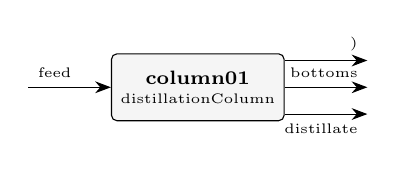
\begin{tikzpicture}[>={Stealth[length=2mm]}, every node/.style={font=\scriptsize}]
  \node[draw, rounded corners=2pt, align=center, minimum width=1.9cm, minimum height=0.85cm, fill=black!4] (column01) at (0.0,-0.0) {\textbf{column01}\\[-1pt]{\tiny distillationColumn}};
  \draw[->] ($(column01.west)+(-1.05,0.00)$) -- ($(column01.west)+(0,0.00)$) node[at start, above, font=\tiny, anchor=south west] {feed};
  \draw[->] ($(column01.east)+(0,-0.34)$) -- ($(column01.east)+(1.05,-0.34)$) node[at end, below, font=\tiny, anchor=north east] {distillate};
  \draw[->] ($(column01.east)+(0,0.00)$) -- ($(column01.east)+(1.05,0.00)$) node[at end, above, font=\tiny, anchor=south east] {bottoms};
  \draw[->] ($(column01.east)+(0,0.34)$) -- ($(column01.east)+(1.05,0.34)$) node[at end, above, font=\tiny, anchor=south east] {)};
\end{tikzpicture}
\end{tutscheme}
\tutwhat{Benzene/toluene distillation column (Wang-Henke)}
\begin{tutnarrative}
- Choupo -$\ast$--------------------------------$\ast$ | \textbackslash\{\}|/ C hemicals | Choupo: open-source, glass-box simulation | | \textbackslash\{\}\textbackslash\{\}|// H eat-transfer | Version: Choupo-dev | | \textbackslash\{\}\textbackslash\{\}\textbackslash\{\}|/// O perations | Website: https://choupo.org | | \textbackslash\{\}\textbackslash\{\}|// U nits | Licence: GPL-3.0-or-later | | \textbackslash\{\}|/ P roperties | Tutorial case file -- part of Choupo | | | O ptimization | |

\end{tutnarrative}
\begin{tutgolden}
\goldrow{kpi}{column01}{T\_top}{354.21089412}
\goldrow{kpi}{column01}{T\_bottom}{382.893530951}
\goldrow{kpi}{column01}{x\_D\_LK}{0.981245045999}
\goldrow{kpi}{column01}{x\_B\_HK}{0.981245183716}
\goldrow{utility}{column01}{heating.steamLP.duty\_kW}{1279.30480005}
\goldrow{utility}{column01}{heating.steamLP.T}{382.893530951}
\goldrow{utility}{column01}{heating.steamLP.kg\_s}{0.585226349518}
\goldrow{utility}{column01}{heating.steamLP.eur\_h}{55.265967362}
\goldrow{utility}{column01}{cooling.coolingWater.duty\_kW}{-1281.04348002}
\goldrow{utility}{column01}{cooling.coolingWater.T}{354.21089412}
\goldrow{utility}{column01}{cooling.coolingWater.kg\_s}{30.6469732063}
\goldrow{utility}{column01}{cooling.coolingWater.eur\_h}{1.84470261124}
\end{tutgolden}

\clearpage
\tutentry{column02\_simultaneous}{tutorials/steady/distillation/column02\_simultaneous}
\begin{tutscheme}
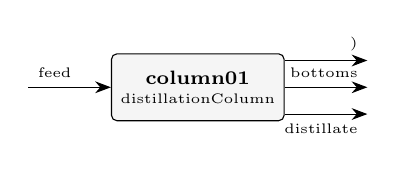
\begin{tikzpicture}[>={Stealth[length=2mm]}, every node/.style={font=\scriptsize}]
  \node[draw, rounded corners=2pt, align=center, minimum width=1.9cm, minimum height=0.85cm, fill=black!4] (column01) at (0.0,-0.0) {\textbf{column01}\\[-1pt]{\tiny distillationColumn}};
  \draw[->] ($(column01.west)+(-1.05,0.00)$) -- ($(column01.west)+(0,0.00)$) node[at start, above, font=\tiny, anchor=south west] {feed};
  \draw[->] ($(column01.east)+(0,-0.34)$) -- ($(column01.east)+(1.05,-0.34)$) node[at end, below, font=\tiny, anchor=north east] {distillate};
  \draw[->] ($(column01.east)+(0,0.00)$) -- ($(column01.east)+(1.05,0.00)$) node[at end, above, font=\tiny, anchor=south east] {bottoms};
  \draw[->] ($(column01.east)+(0,0.34)$) -- ($(column01.east)+(1.05,0.34)$) node[at end, above, font=\tiny, anchor=south east] {)};
\end{tikzpicture}
\end{tutscheme}
\tutwhat{Rigorous distillation by simultaneous MESH Newton (benzene/toluene; validates against column01)}
\begin{tutnarrative}
- Choupo -$\ast$--------------------------------$\ast$ | \textbackslash\{\}|/ C hemicals | Choupo: open-source, glass-box simulation | | \textbackslash\{\}\textbackslash\{\}|// H eat-transfer | Version: Choupo-dev | | \textbackslash\{\}\textbackslash\{\}\textbackslash\{\}|/// O perations | Website: https://choupo.org | | \textbackslash\{\}\textbackslash\{\}|// U nits | Licence: GPL-3.0-or-later | | \textbackslash\{\}|/ P roperties | Tutorial case file -- part of Choupo | | | O ptimization | |

\end{tutnarrative}
\begin{tutgolden}
\goldrow{stream}{bottoms}{F}{0.0138888888889}
\goldrow{stream}{distillate}{F}{0.0138888888889}
\goldrow{stream}{feed}{F}{0.0277777777778}
\goldrow{kpi}{column01}{B}{0.0138888888889}
\goldrow{kpi}{column01}{D}{0.0138888888889}
\goldrow{kpi}{column01}{R}{2}
\goldrow{kpi}{column01}{T\_bottom}{382.893527916}
\goldrow{kpi}{column01}{T\_top}{354.210890137}
\goldrow{kpi}{column01}{feedStage}{8}
\goldrow{kpi}{column01}{nStages}{15}
\goldrow{kpi}{column01}{x\_B\_HK}{0.981245125322}
\goldrow{kpi}{column01}{x\_D\_LK}{0.981245125322}
\goldrow{utility}{column01}{heating.steamLP.duty\_kW}{1299.61040477}
\goldrow{utility}{column01}{heating.steamLP.T}{382.893527916}
\goldmore{6}
\end{tutgolden}

\clearpage
\tutentry{column03\_azeotrope\_mesh}{tutorials/steady/distillation/column03\_azeotrope\_mesh}
\begin{tutscheme}
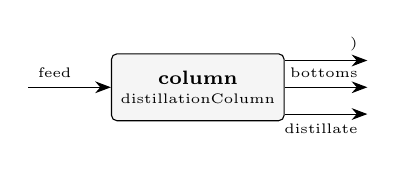
\begin{tikzpicture}[>={Stealth[length=2mm]}, every node/.style={font=\scriptsize}]
  \node[draw, rounded corners=2pt, align=center, minimum width=1.9cm, minimum height=0.85cm, fill=black!4] (column) at (0.0,-0.0) {\textbf{column}\\[-1pt]{\tiny distillationColumn}};
  \draw[->] ($(column.west)+(-1.05,0.00)$) -- ($(column.west)+(0,0.00)$) node[at start, above, font=\tiny, anchor=south west] {feed};
  \draw[->] ($(column.east)+(0,-0.34)$) -- ($(column.east)+(1.05,-0.34)$) node[at end, below, font=\tiny, anchor=north east] {distillate};
  \draw[->] ($(column.east)+(0,0.00)$) -- ($(column.east)+(1.05,0.00)$) node[at end, above, font=\tiny, anchor=south east] {bottoms};
  \draw[->] ($(column.east)+(0,0.34)$) -- ($(column.east)+(1.05,0.34)$) node[at end, above, font=\tiny, anchor=south east] {)};
\end{tikzpicture}
\end{tutscheme}
\tutwhat{Azeotropic distillation (ethanol/water, NRTL) by the rigorous simultaneous MESH method}
\begin{tutnarrative}
- Choupo -$\ast$--------------------------------$\ast$ | \textbackslash\{\}|/ C hemicals | Choupo: open-source, glass-box simulation | | \textbackslash\{\}\textbackslash\{\}|// H eat-transfer | Version: Choupo-dev | | \textbackslash\{\}\textbackslash\{\}\textbackslash\{\}|/// O perations | Website: https://choupo.org | | \textbackslash\{\}\textbackslash\{\}|// U nits | Licence: GPL-3.0-or-later | | \textbackslash\{\}|/ P roperties | Tutorial case file -- part of Choupo | | | O ptimization | |

\end{tutnarrative}
\begin{tutgolden}
\goldrow{stream}{bottoms}{F}{0.0208333333333}
\goldrow{stream}{distillate}{F}{0.00694444444444}
\goldrow{stream}{feed}{F}{0.0277777777778}
\goldrow{kpi}{column}{B}{0.0208333333333}
\goldrow{kpi}{column}{D}{0.00694444444444}
\goldrow{kpi}{column}{R}{2.5}
\goldrow{kpi}{column}{T\_bottom}{357.713408957}
\goldrow{kpi}{column}{T\_top}{351.388958309}
\goldrow{kpi}{column}{feedStage}{8}
\goldrow{kpi}{column}{nStages}{16}
\goldrow{kpi}{column}{x\_B\_HK}{0.868205515093}
\goldrow{kpi}{column}{x\_D\_LK}{0.804616545279}
\goldrow{utility}{column}{heating.steamLP.duty\_kW}{935.650111764}
\goldrow{utility}{column}{heating.steamLP.T}{357.713408957}
\goldmore{6}
\end{tutgolden}

\clearpage
\tutentry{column04\_multifeed\_sidedraw}{tutorials/steady/distillation/column04\_multifeed\_sidedraw}
\begin{tutscheme}
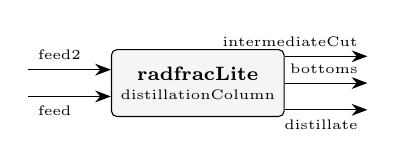
\begin{tikzpicture}[>={Stealth[length=2mm]}, every node/.style={font=\scriptsize}]
  \node[draw, rounded corners=2pt, align=center, minimum width=1.9cm, minimum height=0.85cm, fill=black!4] (radfracLite) at (0.0,-0.0) {\textbf{radfracLite}\\[-1pt]{\tiny distillationColumn}};
  \draw[->] ($(radfracLite.west)+(-1.05,-0.17)$) -- ($(radfracLite.west)+(0,-0.17)$) node[at start, below, font=\tiny, anchor=north west] {feed};
  \draw[->] ($(radfracLite.west)+(-1.05,0.17)$) -- ($(radfracLite.west)+(0,0.17)$) node[at start, above, font=\tiny, anchor=south west] {feed2};
  \draw[->] ($(radfracLite.east)+(0,-0.34)$) -- ($(radfracLite.east)+(1.05,-0.34)$) node[at end, below, font=\tiny, anchor=north east] {distillate};
  \draw[->] ($(radfracLite.east)+(0,0.00)$) -- ($(radfracLite.east)+(1.05,0.00)$) node[at end, above, font=\tiny, anchor=south east] {bottoms};
  \draw[->] ($(radfracLite.east)+(0,0.34)$) -- ($(radfracLite.east)+(1.05,0.34)$) node[at end, above, font=\tiny, anchor=south east] {intermediateCut};
\end{tikzpicture}
\end{tutscheme}
\tutwhat{Simultaneous MESH column: two feeds + a liquid side draw (rigorous MESH)}
\begin{tutnarrative}
- Choupo -$\ast$--------------------------------$\ast$ | \textbackslash\{\}|/ C hemicals | Choupo: open-source, glass-box simulation | | \textbackslash\{\}\textbackslash\{\}|// H eat-transfer | Version: Choupo-dev | | \textbackslash\{\}\textbackslash\{\}\textbackslash\{\}|/// O perations | Website: https://choupo.org | | \textbackslash\{\}\textbackslash\{\}|// U nits | Licence: GPL-3.0-or-later | | \textbackslash\{\}|/ P roperties | Tutorial case file -- part of Choupo | | | O ptimization | |

\end{tutnarrative}
\tutreadme{The rigorous simultaneous MESH column extended to multiple feeds and side draws --- the most-used features of a commercial simulator column, on the glass-box Newton solver.}
\tutreadme{A benzene / toluene / o-xylene split (light / intermediate / heavy):}
\tutreadme{- primary feed --- 100 kmol/h, benzene/toluene/o-xylene 0.40/0.40/0.20, enters high (stage 5); - second feed --- 60 kmol/h, heavier (0.05/0.45/0.50), enters low (stage 11); - liquid side draw --- 15 kmol/h pulled from stage 8, between the two feeds.}
\tutreadme{Mass closes (100 + 60 = 42 + 15 + 103 = 160 kmol/h). Q\_condenser = -1436 kW, Q\_reboiler = +1527 kW. The side draw does exactly what it should --- bleed the intermediate component where it is most enriched on the trays.}
\tutreadme{The simultaneous MESH is a bubble-point-reduced Newton (CMO flows). The extension generalises the single fixed feed into a per-stage flow staircase: L[j], V[j] are rebuilt by a CMO march that adds each feed's liquid/vapour parts and subtracts each draw; every stage's material balance carries an F\_j z\_\{F,j\} source and (L\_j+U\_j), (V\_j+W\_j) outflows. The general balance reduces exactly to the old single-feed equations when there is one feed and no draw --- so every existing distillation tutorial is unchanged (verified).}
\tutreadme{outputs ( distillate bottoms <draw1> <draw2> ... ) --- side-draw streams follow distillate and bottoms, in stage order.}
\begin{tutgolden}
\goldrow{stream}{bottoms}{F}{0.0286111111111}
\goldrow{stream}{distillate}{F}{0.0116666666667}
\goldrow{stream}{feed}{F}{0.0277777777778}
\goldrow{stream}{intermediateCut}{F}{0.00416666666667}
\goldrow{kpi}{radfracLite}{B}{0.0286111111111}
\goldrow{kpi}{radfracLite}{D}{0.0116666666667}
\goldrow{kpi}{radfracLite}{Q\_condenser\_kW}{-1435.80274013}
\goldrow{kpi}{radfracLite}{Q\_reboiler\_kW}{1516.14164522}
\goldrow{kpi}{radfracLite}{R}{3}
\goldrow{kpi}{radfracLite}{T\_bottom}{395.926996928}
\goldrow{kpi}{radfracLite}{T\_top}{354.978489481}
\goldrow{kpi}{radfracLite}{feedStage}{5}
\goldrow{kpi}{radfracLite}{nFeeds}{2}
\goldrow{kpi}{radfracLite}{nSideDraws}{1}
\goldmore{11}
\end{tutgolden}

\clearpage
\tutentry{column05\_reactive\_methylacetate}{tutorials/steady/distillation/column05\_reactive\_methylacetate}
\begin{tutscheme}
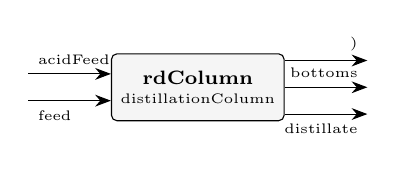
\begin{tikzpicture}[>={Stealth[length=2mm]}, every node/.style={font=\scriptsize}]
  \node[draw, rounded corners=2pt, align=center, minimum width=1.9cm, minimum height=0.85cm, fill=black!4] (rdColumn) at (0.0,-0.0) {\textbf{rdColumn}\\[-1pt]{\tiny distillationColumn}};
  \draw[->] ($(rdColumn.west)+(-1.05,-0.17)$) -- ($(rdColumn.west)+(0,-0.17)$) node[at start, below, font=\tiny, anchor=north west] {feed};
  \draw[->] ($(rdColumn.west)+(-1.05,0.17)$) -- ($(rdColumn.west)+(0,0.17)$) node[at start, above, font=\tiny, anchor=south west] {acidFeed};
  \draw[->] ($(rdColumn.east)+(0,-0.34)$) -- ($(rdColumn.east)+(1.05,-0.34)$) node[at end, below, font=\tiny, anchor=north east] {distillate};
  \draw[->] ($(rdColumn.east)+(0,0.00)$) -- ($(rdColumn.east)+(1.05,0.00)$) node[at end, above, font=\tiny, anchor=south east] {bottoms};
  \draw[->] ($(rdColumn.east)+(0,0.34)$) -- ($(rdColumn.east)+(1.05,0.34)$) node[at end, above, font=\tiny, anchor=south east] {)};
\end{tikzpicture}
\end{tutscheme}
\tutwhat{Reactive distillation: methyl acetate synthesis (validation vs P?pken et al. 2001, run S-1)}
\begin{tutnarrative}
- Choupo -$\ast$--------------------------------$\ast$ | \textbackslash\{\}|/ C hemicals | Choupo: open-source, glass-box simulation | | \textbackslash\{\}\textbackslash\{\}|// H eat-transfer | Version: Choupo-dev | | \textbackslash\{\}\textbackslash\{\}\textbackslash\{\}|/// O perations | Website: https://choupo.org | | \textbackslash\{\}\textbackslash\{\}|// U nits | Licence: GPL-3.0-or-later | | \textbackslash\{\}|/ P roperties | Tutorial case file -- part of Choupo | | | O ptimization | |

\end{tutnarrative}
\tutreadme{The simultaneous MESH column with an equilibrium reaction on the catalytic stages (rigorous column rung 4), compared to a published experiment.}
\tutreadme{Mole-conserving, so the CMO internal-flow profile is untouched. Each catalytic stage carries one extra unknown --- the molar extent ?\_j --- closed by the activity-based equilibrium residual $\Sigma$\_i $\nu$\_i ln($\gamma$\_i x\_i) = ln K\_a(T), with $\gamma$\_i from the liquid activity model and K\_a(T) by van't Hoff: K\_a(T) = K\_a(298)$\cdot$exp(-$\Delta$h$^\circ$\_r/R$\cdot$(1/T - 1/298.15)). Converged by homotopy (solve non-reactive, then switch the reaction on).}
\tutreadme{> T. P?pken, S. Steinigeweg \& J. Gmehling, $\ast$"Synthesis and Hydrolysis of > Methyl Acetate by Reactive Distillation\textbackslash\{\}ldots"$\ast$, Ind. Eng. Chem. Res. 40 > (2001) 1566. Run S-1: N = 25, reactive stages 11--19, HOAc fed above / > MeOH below the zone, reflux 2.1, P $\approx$ 1.017 bar. Measured endpoints, cited, in > constant/experimental/methyl\_acetate\_RD\_profile.csv.}
\tutreadme{The equilibrium constant and thermodynamics are from the companion paper P?pken, G?tze \& Gmehling, Ind. Eng. Chem. Res. 39 (2000) 2601: K\_a(298) $\approx$ 38.7, $\Delta$h$^\circ$\_r $\approx$ -5.67 kJ/mol $\to$ K\_a $\approx$ 29 in the reactive zone (\textasciitilde{}65 $^\circ$C).}
\tutreadme{This is not a tight match, and the reason is physically important: with the correct equilibrium K\_a ($\approx$29) the model gives the equilibrium ceiling (96 \%), and it correctly brackets the measurement from above. The measured 87.6 \% is $\ast$below$\ast$ the equilibrium because the real column is kinetically limited --- the paper's recommended model is an adsorption-based finite $\ast$rate$\ast$ (per gram of catalyst), not equilibrium. An earlier run with an (incorrect, too low) K\_a = 5.2 gave 90.7 \%, a closer $\ast$number$\ast$ but for the wrong reason; using a wrong constant to fake agreement would be dishonest.}
\tutreadme{So the path to a bit-tight match is the kinetic rate model, not the thermo.}
\begin{tutgolden}
\goldrow{stream}{bottoms}{F}{9.13888888889e-06}
\goldrow{stream}{distillate}{F}{8.36111111111e-06}
\goldrow{stream}{feed}{F}{8.94444444444e-06}
\goldrow{kpi}{rdColumn}{B}{9.13888888889e-06}
\goldrow{kpi}{rdColumn}{D}{8.36111111111e-06}
\goldrow{kpi}{rdColumn}{Q\_condenser\_kW}{-0.790521316742}
\goldrow{kpi}{rdColumn}{Q\_reboiler\_kW}{0.626813788646}
\goldrow{kpi}{rdColumn}{R}{2.1}
\goldrow{kpi}{rdColumn}{T\_bottom}{363.229492539}
\goldrow{kpi}{rdColumn}{T\_top}{330.062558898}
\goldrow{kpi}{rdColumn}{conversion}{0.960508806863}
\goldrow{kpi}{rdColumn}{feedStage}{20}
\goldrow{kpi}{rdColumn}{nFeeds}{2}
\goldrow{kpi}{rdColumn}{nSideDraws}{0}
\goldmore{12}
\end{tutgolden}

\clearpage
\tutentry{column06\_fullMESH}{tutorials/steady/distillation/column06\_fullMESH}
\begin{tutscheme}
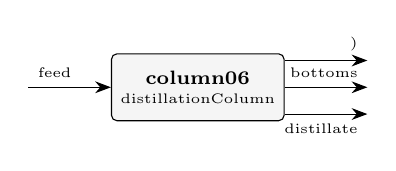
\begin{tikzpicture}[>={Stealth[length=2mm]}, every node/.style={font=\scriptsize}]
  \node[draw, rounded corners=2pt, align=center, minimum width=1.9cm, minimum height=0.85cm, fill=black!4] (column06) at (0.0,-0.0) {\textbf{column06}\\[-1pt]{\tiny distillationColumn}};
  \draw[->] ($(column06.west)+(-1.05,0.00)$) -- ($(column06.west)+(0,0.00)$) node[at start, above, font=\tiny, anchor=south west] {feed};
  \draw[->] ($(column06.east)+(0,-0.34)$) -- ($(column06.east)+(1.05,-0.34)$) node[at end, below, font=\tiny, anchor=north east] {distillate};
  \draw[->] ($(column06.east)+(0,0.00)$) -- ($(column06.east)+(1.05,0.00)$) node[at end, above, font=\tiny, anchor=south east] {bottoms};
  \draw[->] ($(column06.east)+(0,0.34)$) -- ($(column06.east)+(1.05,0.34)$) node[at end, above, font=\tiny, anchor=south east] {)};
\end{tikzpicture}
\end{tutscheme}
\tutwhat{Full-MESH (Naphtali-Sandholm) distillation -- energy-consistent V\_j/L\_j, seeded from the CMO solution (benzene/toluene; compare column02)}
\begin{tutnarrative}
- Choupo -$\ast$--------------------------------$\ast$ | \textbackslash\{\}|/ C hemicals | Choupo: open-source, glass-box simulation | | \textbackslash\{\}\textbackslash\{\}|// H eat-transfer | Version: Choupo-dev | | \textbackslash\{\}\textbackslash\{\}\textbackslash\{\}|/// O perations | Website: https://choupo.org | | \textbackslash\{\}\textbackslash\{\}|// U nits | Licence: GPL-3.0-or-later | | \textbackslash\{\}|/ P roperties | Tutorial case file -- part of Choupo | | | O ptimization | |

\end{tutnarrative}
\tutreadme{The same benzene/toluene column as column02\_simultaneous, but solved by the full MESH (model fullMESH) instead of the bubble-point/CMO reduction.}
\tutreadme{The simultaneous method is a bubble-point-reduced MESH: it assumes constant molal overflow (CMO --- equimolal latent heats), so the internal vapour/liquid flows V\_j, L\_j are fixed by a mass march and only the compositions x\_j and stage temperatures T\_j are solved.}
\tutreadme{The full MESH (Naphtali--Sandholm) promotes V\_j and L\_j to unknowns and adds, per stage, the total-mass balance and the energy balance --- so the flows follow the $\ast$real$\ast$ latent heats instead of assuming them equal. The extra per-stage energy equation is the enthalpy residual the CMO never carried:}
\tutreadme{Total condenser: V\_0 = 0, L\_0 = R$\cdot$D; reboiler: L\_\{N-1\} = B; their energy balances give Q\_cond / Q\_reb as results.}
\tutreadme{The full-MESH is seeded from the converged CMO profile --- the cheap model launches the rigorous one. Here it converges in \textasciitilde{}4 Newton iterations from that seed (it would be far harder from a cold start).}
\tutreadme{Benzene ($\Delta$h\_vap $\approx$ 30.8 kJ/mol) and toluene ($\approx$ 33.2 kJ/mol) have similar latent heats, so CMO is a good approximation and the two answers nearly coincide --- the \textasciitilde{}0.002 / \textasciitilde{}0.1 K gap IS the energy-balance correction the full-MESH makes and the CMO drops. On a wide-boiling column (a depropaniser) the gap is much larger; that is where the full-MESH earns its cost.}
\begin{tutgolden}
\goldrow{stream}{bottoms}{F}{0.0138888888889}
\goldrow{stream}{distillate}{F}{0.0138888888889}
\goldrow{stream}{feed}{F}{0.0277777777778}
\goldrow{kpi}{column06}{B}{0.0138888888889}
\goldrow{kpi}{column06}{D}{0.0138888888889}
\goldrow{kpi}{column06}{Q\_condenser\_kW}{-1281.19539111}
\goldrow{kpi}{column06}{Q\_reboiler\_kW}{1299.72437334}
\goldrow{kpi}{column06}{R}{2}
\goldrow{kpi}{column06}{T\_bottom}{382.774927808}
\goldrow{kpi}{column06}{T\_top}{354.339103085}
\goldrow{kpi}{column06}{feedStage}{8}
\goldrow{kpi}{column06}{nFeeds}{1}
\goldrow{kpi}{column06}{nSideDraws}{0}
\goldrow{kpi}{column06}{nStages}{15}
\goldmore{10}
\end{tutgolden}

\clearpage
\tutentry{column07\_naphtaliSandholm}{tutorials/steady/distillation/column07\_naphtaliSandholm}
\begin{tutscheme}
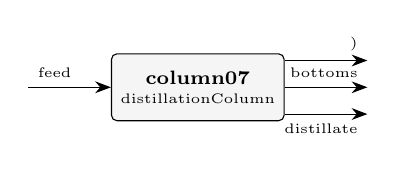
\begin{tikzpicture}[>={Stealth[length=2mm]}, every node/.style={font=\scriptsize}]
  \node[draw, rounded corners=2pt, align=center, minimum width=1.9cm, minimum height=0.85cm, fill=black!4] (column07) at (0.0,-0.0) {\textbf{column07}\\[-1pt]{\tiny distillationColumn}};
  \draw[->] ($(column07.west)+(-1.05,0.00)$) -- ($(column07.west)+(0,0.00)$) node[at start, above, font=\tiny, anchor=south west] {feed};
  \draw[->] ($(column07.east)+(0,-0.34)$) -- ($(column07.east)+(1.05,-0.34)$) node[at end, below, font=\tiny, anchor=north east] {distillate};
  \draw[->] ($(column07.east)+(0,0.00)$) -- ($(column07.east)+(1.05,0.00)$) node[at end, above, font=\tiny, anchor=south east] {bottoms};
  \draw[->] ($(column07.east)+(0,0.34)$) -- ($(column07.east)+(1.05,0.34)$) node[at end, above, font=\tiny, anchor=south east] {)};
\end{tikzpicture}
\end{tutscheme}
\tutwhat{Full-MESH (Naphtali-Sandholm) validation vs AIChE J. 17 (1971) 148, Problem 2: nC4/iC5/nC5}
\begin{tutnarrative}
- Choupo -$\ast$--------------------------------$\ast$ VALIDATION -- Naphtali \& Sandholm, AIChE Journal 17(1), 148-153 (1971), DOI 10.1002/aic.690170130, Problem 2 (ideal hydrocarbon distillation). 20 plates; liquid feed (T = 30 F = 272.04 K, 500 mol each of nC4/iC5/nC5) on plate 10; reflux ratio 1000; 80\% recovered in bottoms (B = 1200). A liquid sidestream on plate 1 (condenser) takes 30\% of the reflux.

EQUIVALENT SPEC (same internal flows, no condenser sidestream): the distillate and the sidestream leave the total condenser with the SAME composition, so they are combined into ONE top product of 300 with reflux R = L1/300 = 996.68/300 = 3.3223. This gives identical L1 = 996.68 and V2 = 1296.68, hence the same column.

Paper result: B = nC4 200.1 / iC5 499.9 / nC5 500.0; combined top \textasciitilde{} 99.97\% nC4; plate T 29.7 F (top) $\to$ 77.0 F (reboiler) \textasciitilde{} 272.0 $\to$ 298.2 K.

\end{tutnarrative}
\tutreadme{Reproduces the ideal-hydrocarbon distillation of Naphtali \& Sandholm, "Multicomponent Separation Calculations by Linearization", AIChE Journal 17(1), 148--153 (1971) --- DOI [10.1002/aic.690170130](https://doi.org/10.1002/aic.690170130) --- the paper that introduced the very full-MESH method Choupo's model fullMESH implements.}
\tutreadme{n-butane / isopentane / n-pentane, 20 plates, liquid feed (T = 30 $^\circ$F = 272.04 K, 500 mol of each) on plate 10, reflux ratio 1000, 80 \% of the feed recovered in the bottoms (B = 1200). A liquid sidestream on plate 1 (the condenser) takes 30 \% of the reflux.}
\tutreadme{Equivalent spec used here. The distillate ($\approx$1) and the condenser sidestream ($\approx$299) leave the $\ast$total$\ast$ condenser with the same composition, so they are combined into ONE top product of 300 with reflux R = L$_1$/300 = 996.68/300 = 3.3223. This gives identical internal flows (L$_1$ = 996.68, V$_2$ = 1296.68), hence the identical column --- without needing a condenser side draw.}
\tutreadme{Converges in 3 full-MESH Newton iterations (seeded from the CMO profile).}
\tutreadme{Products Choupo ------ top product (300) 99.99 \% n-C$_4$ bottoms n-C$_4$ / i-C$_5$ / n-C$_5$ 200 / 500 / 500 B 1200}
\tutreadme{The profile shape --- the flat n-butane-rich top, the sharp rise across the feed zone, the pentane-plateau, the reboiler climb --- matches stage-by-stage. The \textasciitilde{}1--2 K residual is thermo, not method: Choupo uses fitted Antoine vapour pressures, the paper used the K-value tables in Brown's $\ast$Unit Operations$\ast$ (1950).}
\begin{tutgolden}
\goldrow{stream}{feed}{F}{0.416666666667}
\goldrow{kpi}{column07}{B}{0.333333333333}
\goldrow{kpi}{column07}{D}{0.0833333333333}
\goldrow{kpi}{column07}{Q\_condenser\_kW}{-8082.6120755}
\goldrow{kpi}{column07}{Q\_reboiler\_kW}{9374.37429576}
\goldrow{kpi}{column07}{R}{3.3223}
\goldrow{kpi}{column07}{T\_bottom}{296.58946842}
\goldrow{kpi}{column07}{T\_top}{272.663334648}
\goldrow{kpi}{column07}{feedStage}{10}
\goldrow{kpi}{column07}{nFeeds}{1}
\goldrow{kpi}{column07}{nSideDraws}{0}
\goldrow{kpi}{column07}{nStages}{20}
\goldrow{kpi}{column07}{x\_B\_HK}{0.416665691626}
\goldrow{kpi}{column07}{x\_D\_LK}{0.999874145869}
\goldmore{5}
\end{tutgolden}

\clearpage
\tutentry{column08\_radfrac\_multidraw}{tutorials/steady/distillation/column08\_radfrac\_multidraw}
\begin{tutscheme}
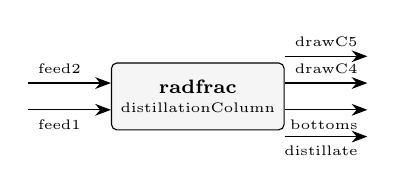
\begin{tikzpicture}[>={Stealth[length=2mm]}, every node/.style={font=\scriptsize}]
  \node[draw, rounded corners=2pt, align=center, minimum width=1.9cm, minimum height=0.85cm, fill=black!4] (radfrac) at (0.0,-0.0) {\textbf{radfrac}\\[-1pt]{\tiny distillationColumn}};
  \draw[->] ($(radfrac.west)+(-1.05,-0.17)$) -- ($(radfrac.west)+(0,-0.17)$) node[at start, below, font=\tiny, anchor=north west] {feed1};
  \draw[->] ($(radfrac.west)+(-1.05,0.17)$) -- ($(radfrac.west)+(0,0.17)$) node[at start, above, font=\tiny, anchor=south west] {feed2};
  \draw[->] ($(radfrac.east)+(0,-0.51)$) -- ($(radfrac.east)+(1.05,-0.51)$) node[at end, below, font=\tiny, anchor=north east] {distillate};
  \draw[->] ($(radfrac.east)+(0,-0.17)$) -- ($(radfrac.east)+(1.05,-0.17)$) node[at end, below, font=\tiny, anchor=north east] {bottoms};
  \draw[->] ($(radfrac.east)+(0,0.17)$) -- ($(radfrac.east)+(1.05,0.17)$) node[at end, above, font=\tiny, anchor=south east] {drawC4};
  \draw[->] ($(radfrac.east)+(0,0.51)$) -- ($(radfrac.east)+(1.05,0.51)$) node[at end, above, font=\tiny, anchor=south east] {drawC5};
\end{tikzpicture}
\end{tutscheme}
\tutwhat{rigorous column: multi-feed + multi-side-draw distillation (C3/C4/C5/C6), full-MESH}
\begin{tutnarrative}
- Choupo -$\ast$--------------------------------$\ast$ Multi-feed, multi-side-draw rigorous column (the most-used rigorous column features at once). A C3/C4/C5/C6 mix split FOUR ways: distillate \textasciitilde{} propane, an upper liquid side draw \textasciitilde{} n-butane, a lower liquid side draw \textasciitilde{} n-pentane, bottoms \textasciitilde{} n-hexane. TWO feeds enter at different heights (a light cut high, a heavy cut low) -- so the column sees the realistic case of feeds of different composition. Feeds are flowsheet STREAMS (`inputs (...)`) so the plant-boundary mass+energy balance sees them (information follows the streams). Validation reference (propose): Hofeling \& Seader, AIChE J. 24(6) (1978), DOI 10.1002/aic.690240631 -- the Naphtali-Sandholm extension for general multi-feed / multi-draw / interlinked separators.

\end{tutnarrative}
\tutreadme{A C3/C4/C5/C6 depropanizer-style column at 16 bar, split four ways by the rigorous full-MESH, exercising the two most-used rigorous column features at once: TWO feeds (a light cut high, a heavy cut low) and TWO liquid side draws.}
\tutreadme{Two saturated-liquid feeds (100 kmol/h each, 290 K / 320 K): a light cut on stage 10, a heavy cut on stage 20. 30 stages, R = 4. Mass closes exactly (200 = 45 + 55 + 55 + 45 kmol/h) and the energy balance closes: the feed-to-product enthalpy gap (1137.7 kW) equals the net duty \$Q\_\{\textbackslash\{\}text\{reb\}\}+Q\_\{\textbackslash\{\}text\{cond\}\} = 1942.3 - 804.6\$ kW. Converges in a few full-MESH iterations from the CMO seed.}
\tutreadme{This case was first written at 1 atm, and the energy balance would not close --- because at 1 atm and 290 K the light hydrocarbons (propane b.p. 231 K, n-butane 272 K) are above their boiling points: the feed streams flash to VAPOUR (vf = 1.0), yet the column was told quality 1.0 (saturated liquid). The latent heat of the unrecognised vapour feed was exactly the missing \textasciitilde{}1 MW. At 16 bar the feeds are genuinely liquid (vf = 0, consistent with quality 1.0) and the balance closes --- which is also why a real depropanizer runs at elevated pressure: so the propane distillate condenses against cooling water (here 321.6 K). A feed's thermal state must be specified consistently with its actual phase.}
\tutreadme{Both feeds are real flowsheet streams (inputs ( feed1 feed2 ), mapped to stages by operation.feeds), so the plant-boundary mass + energy balance sees them ($\ast$information follows the streams$\ast$). Side draws are outputs in stage order: outputs ( distillate bottoms drawC4 drawC5 ).}
\tutreadme{Self-consistently validated (mass + energy close, four cuts in volatility order) on the full-MESH solver that IS paper-validated against Naphtali \& Sandholm (1971) in column07\_naphtaliSandholm. No external multi-feed+multi-draw single-column benchmark with published profiles is readily available in the open literature.}
\begin{tutgolden}
\goldrow{stream}{bottoms}{F}{0.0125}
\goldrow{stream}{distillate}{F}{0.0125}
\goldrow{stream}{drawC4}{F}{0.0152777777778}
\goldrow{stream}{drawC5}{F}{0.0152777777778}
\goldrow{stream}{feed1}{F}{0.0277777777778}
\goldrow{stream}{feed2}{F}{0.0277777777778}
\goldrow{kpi}{radfrac}{B}{0.0125}
\goldrow{kpi}{radfrac}{D}{0.0125}
\goldrow{kpi}{radfrac}{Q\_condenser\_kW}{-804.58622364}
\goldrow{kpi}{radfrac}{Q\_reboiler\_kW}{1698.71150765}
\goldrow{kpi}{radfrac}{R}{4}
\goldrow{kpi}{radfrac}{T\_bottom}{454.498489397}
\goldrow{kpi}{radfrac}{T\_top}{321.647346922}
\goldrow{kpi}{radfrac}{feedStage}{10}
\goldmore{13}
\end{tutgolden}

\clearpage
\tutentry{column09\_tray\_hydraulics}{tutorials/steady/distillation/column09\_tray\_hydraulics}
\begin{tutscheme}
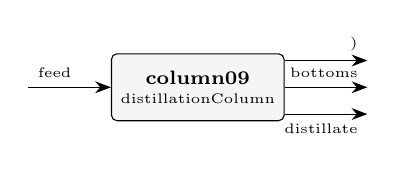
\begin{tikzpicture}[>={Stealth[length=2mm]}, every node/.style={font=\scriptsize}]
  \node[draw, rounded corners=2pt, align=center, minimum width=1.9cm, minimum height=0.85cm, fill=black!4] (column09) at (0.0,-0.0) {\textbf{column09}\\[-1pt]{\tiny distillationColumn}};
  \draw[->] ($(column09.west)+(-1.05,0.00)$) -- ($(column09.west)+(0,0.00)$) node[at start, above, font=\tiny, anchor=south west] {feed};
  \draw[->] ($(column09.east)+(0,-0.34)$) -- ($(column09.east)+(1.05,-0.34)$) node[at end, below, font=\tiny, anchor=north east] {distillate};
  \draw[->] ($(column09.east)+(0,0.00)$) -- ($(column09.east)+(1.05,0.00)$) node[at end, above, font=\tiny, anchor=south east] {bottoms};
  \draw[->] ($(column09.east)+(0,0.34)$) -- ($(column09.east)+(1.05,0.34)$) node[at end, above, font=\tiny, anchor=south east] {)};
\end{tikzpicture}
\end{tutscheme}
\tutwhat{Sieve-tray hydraulics: the column that separates, sized so its trays do not flood}
\begin{tutnarrative}
- Choupo -$\ast$--------------------------------$\ast$ | \textbackslash\{\}|/ C hemicals | Choupo: open-source, glass-box simulation | | \textbackslash\{\}\textbackslash\{\}|// H eat-transfer | Version: Choupo-dev | | \textbackslash\{\}\textbackslash\{\}\textbackslash\{\}|/// O perations | Website: https://choupo.org | | \textbackslash\{\}\textbackslash\{\}|// U nits | Licence: GPL-3.0-or-later | | \textbackslash\{\}|/ P roperties | Tutorial case file -- part of Choupo | | | O ptimization | |

\end{tutnarrative}
\begin{tutgolden}
\goldrow{stream}{bottoms}{F}{0.0138888888889}
\goldrow{stream}{distillate}{F}{0.0138888888889}
\goldrow{stream}{feed}{F}{0.0277777777778}
\goldrow{kpi}{column09}{B}{0.0138888888889}
\goldrow{kpi}{column09}{D}{0.0138888888889}
\goldrow{kpi}{column09}{L\_rect}{0.0277777777778}
\goldrow{kpi}{column09}{L\_strip}{0.0555555555556}
\goldrow{kpi}{column09}{Q\_condenser\_kW}{-1281.04348002}
\goldrow{kpi}{column09}{Q\_reboiler\_kW}{1279.30480005}
\goldrow{kpi}{column09}{R}{2}
\goldrow{kpi}{column09}{T\_bottom}{382.893530951}
\goldrow{kpi}{column09}{T\_top}{354.21089412}
\goldrow{kpi}{column09}{V\_rect}{0.0416666666667}
\goldrow{kpi}{column09}{V\_strip}{0.0416666666667}
\goldmore{19}
\end{tutgolden}

\clearpage
\tutentry{column10\_flooding}{tutorials/steady/distillation/column10\_flooding}
\begin{tutscheme}
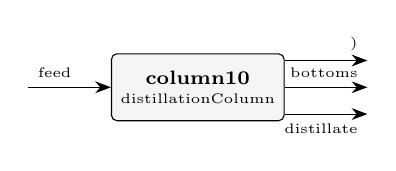
\begin{tikzpicture}[>={Stealth[length=2mm]}, every node/.style={font=\scriptsize}]
  \node[draw, rounded corners=2pt, align=center, minimum width=1.9cm, minimum height=0.85cm, fill=black!4] (column10) at (0.0,-0.0) {\textbf{column10}\\[-1pt]{\tiny distillationColumn}};
  \draw[->] ($(column10.west)+(-1.05,0.00)$) -- ($(column10.west)+(0,0.00)$) node[at start, above, font=\tiny, anchor=south west] {feed};
  \draw[->] ($(column10.east)+(0,-0.34)$) -- ($(column10.east)+(1.05,-0.34)$) node[at end, below, font=\tiny, anchor=north east] {distillate};
  \draw[->] ($(column10.east)+(0,0.00)$) -- ($(column10.east)+(1.05,0.00)$) node[at end, above, font=\tiny, anchor=south east] {bottoms};
  \draw[->] ($(column10.east)+(0,0.34)$) -- ($(column10.east)+(1.05,0.34)$) node[at end, above, font=\tiny, anchor=south east] {)};
\end{tikzpicture}
\end{tutscheme}
\tutwhat{The same column, built too narrow: every tray floods -- and it still converges}
\begin{tutnarrative}
- Choupo -$\ast$--------------------------------$\ast$ | \textbackslash\{\}|/ C hemicals | Choupo: open-source, glass-box simulation | | \textbackslash\{\}\textbackslash\{\}|// H eat-transfer | Version: Choupo-dev | | \textbackslash\{\}\textbackslash\{\}\textbackslash\{\}|/// O perations | Website: https://choupo.org | | \textbackslash\{\}\textbackslash\{\}|// U nits | Licence: GPL-3.0-or-later | | \textbackslash\{\}|/ P roperties | Tutorial case file -- part of Choupo | | | O ptimization | |

\end{tutnarrative}
\begin{tutgolden}
\goldrow{stream}{bottoms}{F}{0.0138888888889}
\goldrow{stream}{distillate}{F}{0.0138888888889}
\goldrow{stream}{feed}{F}{0.0277777777778}
\goldrow{kpi}{column10}{B}{0.0138888888889}
\goldrow{kpi}{column10}{D}{0.0138888888889}
\goldrow{kpi}{column10}{L\_rect}{0.0277777777778}
\goldrow{kpi}{column10}{L\_strip}{0.0555555555556}
\goldrow{kpi}{column10}{Q\_condenser\_kW}{-1281.04348002}
\goldrow{kpi}{column10}{Q\_reboiler\_kW}{1279.30480005}
\goldrow{kpi}{column10}{R}{2}
\goldrow{kpi}{column10}{T\_bottom}{382.893530951}
\goldrow{kpi}{column10}{T\_top}{354.21089412}
\goldrow{kpi}{column10}{V\_rect}{0.0416666666667}
\goldrow{kpi}{column10}{V\_strip}{0.0416666666667}
\goldmore{19}
\end{tutgolden}

\clearpage
\tutentry{column11\_murphree}{tutorials/steady/distillation/column11\_murphree}
\begin{tutscheme}
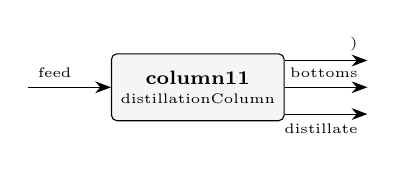
\begin{tikzpicture}[>={Stealth[length=2mm]}, every node/.style={font=\scriptsize}]
  \node[draw, rounded corners=2pt, align=center, minimum width=1.9cm, minimum height=0.85cm, fill=black!4] (column11) at (0.0,-0.0) {\textbf{column11}\\[-1pt]{\tiny distillationColumn}};
  \draw[->] ($(column11.west)+(-1.05,0.00)$) -- ($(column11.west)+(0,0.00)$) node[at start, above, font=\tiny, anchor=south west] {feed};
  \draw[->] ($(column11.east)+(0,-0.34)$) -- ($(column11.east)+(1.05,-0.34)$) node[at end, below, font=\tiny, anchor=north east] {distillate};
  \draw[->] ($(column11.east)+(0,0.00)$) -- ($(column11.east)+(1.05,0.00)$) node[at end, above, font=\tiny, anchor=south east] {bottoms};
  \draw[->] ($(column11.east)+(0,0.34)$) -- ($(column11.east)+(1.05,0.34)$) node[at end, above, font=\tiny, anchor=south east] {)};
\end{tikzpicture}
\end{tutscheme}
\tutwhat{Murphree tray efficiency: 15 REAL trays, not 15 ideal stages -- and the purity you actually get}
\begin{tutnarrative}
- Choupo -$\ast$--------------------------------$\ast$ | \textbackslash\{\}|/ C hemicals | Choupo: open-source, glass-box simulation | | \textbackslash\{\}\textbackslash\{\}|// H eat-transfer | Version: Choupo-dev | | \textbackslash\{\}\textbackslash\{\}\textbackslash\{\}|/// O perations | Website: https://choupo.org | | \textbackslash\{\}\textbackslash\{\}|// U nits | Licence: GPL-3.0-or-later | | \textbackslash\{\}|/ P roperties | Tutorial case file -- part of Choupo | | | O ptimization | |

\end{tutnarrative}
\begin{tutgolden}
\goldrow{stream}{bottoms}{F}{0.0138888888889}
\goldrow{stream}{distillate}{F}{0.0138888888889}
\goldrow{stream}{feed}{F}{0.0277777777778}
\goldrow{kpi}{column11}{B}{0.0138888888889}
\goldrow{kpi}{column11}{D}{0.0138888888889}
\goldrow{kpi}{column11}{L\_rect}{0.0277777777778}
\goldrow{kpi}{column11}{L\_strip}{0.0555555555556}
\goldrow{kpi}{column11}{Q\_condenser\_kW}{-1284.29753602}
\goldrow{kpi}{column11}{Q\_reboiler\_kW}{1281.05938025}
\goldrow{kpi}{column11}{R}{2}
\goldrow{kpi}{column11}{T\_bottom}{381.492133108}
\goldrow{kpi}{column11}{T\_top}{355.136328304}
\goldrow{kpi}{column11}{V\_rect}{0.0416666666667}
\goldrow{kpi}{column11}{V\_strip}{0.0416666666667}
\goldmore{20}
\end{tutgolden}

\clearpage
\tutentry{column12\_stage\_is\_a\_flash}{tutorials/steady/distillation/column12\_stage\_is\_a\_flash}
\begin{tutscheme}
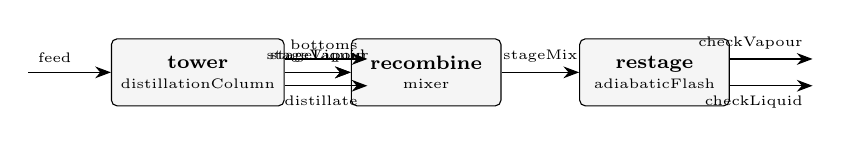
\begin{tikzpicture}[>={Stealth[length=2mm]}, every node/.style={font=\scriptsize}]
  \node[draw, rounded corners=2pt, align=center, minimum width=1.9cm, minimum height=0.85cm, fill=black!4] (tower) at (0.0,-0.0) {\textbf{tower}\\[-1pt]{\tiny distillationColumn}};
  \node[draw, rounded corners=2pt, align=center, minimum width=1.9cm, minimum height=0.85cm, fill=black!4] (recombine) at (2.9,-0.0) {\textbf{recombine}\\[-1pt]{\tiny mixer}};
  \node[draw, rounded corners=2pt, align=center, minimum width=1.9cm, minimum height=0.85cm, fill=black!4] (restage) at (5.8,-0.0) {\textbf{restage}\\[-1pt]{\tiny adiabaticFlash}};
  \draw[->] ($(tower.west)+(-1.05,0.00)$) -- ($(tower.west)+(0,0.00)$) node[at start, above, font=\tiny, anchor=south west] {feed};
  \draw[->] (tower) -- (recombine) node[midway, above, font=\tiny] {stageLiquid};
  \draw[->] (tower) -- (recombine) node[midway, above, font=\tiny] {stageVapour};
  \draw[->] (recombine) -- (restage) node[midway, above, font=\tiny] {stageMix};
  \draw[->] ($(tower.east)+(0,-0.17)$) -- ($(tower.east)+(1.05,-0.17)$) node[at end, below, font=\tiny, anchor=north east] {distillate};
  \draw[->] ($(tower.east)+(0,0.17)$) -- ($(tower.east)+(1.05,0.17)$) node[at end, above, font=\tiny, anchor=south east] {bottoms};
  \draw[->] ($(restage.east)+(0,-0.17)$) -- ($(restage.east)+(1.05,-0.17)$) node[at end, below, font=\tiny, anchor=north east] {checkLiquid};
  \draw[->] ($(restage.east)+(0,0.17)$) -- ($(restage.east)+(1.05,0.17)$) node[at end, above, font=\tiny, anchor=south east] {checkVapour};
\end{tikzpicture}
\end{tutscheme}
\tutwhat{An equilibrium stage IS a flash: a tray's own two products, recombined and re-flashed, must come back as the same tray}
\begin{tutnarrative}
- Choupo -$\ast$--------------------------------$\ast$ | \textbackslash\{\}|/ C hemicals | Choupo: open-source, glass-box simulation | | \textbackslash\{\}\textbackslash\{\}|// H eat-transfer | Version: Choupo-dev | | \textbackslash\{\}\textbackslash\{\}\textbackslash\{\}|/// O perations | Website: https://choupo.org | | \textbackslash\{\}\textbackslash\{\}|// U nits | Licence: GPL-3.0-or-later | | \textbackslash\{\}|/ P roperties | Tutorial case file -- part of Choupo | | | O ptimization | |

\end{tutnarrative}
\tutreadme{What it demonstrates: that Choupo's two independent equilibrium routines --- the column's MESH equations and the flash drum's Rachford-Rice --- give the same answer, by making them say it to each other inside one run.}
\tutreadme{Stage 5 is an equilibrium stage, so the vapour leaving it is in equilibrium with the liquid leaving it. Put them back together, let them separate again at the same pressure with no heat added, and nothing may happen. The run must produce}
\tutreadme{Not one of those numbers is typed into the case. Both sides are computed, by different code, and bin/curate/check\_stage\_identity.py compares them.}
\tutreadme{Three things at once, and each of them has been wrong in a simulator somewhere:}
\tutreadme{1. The K-value definition. The column asks the package for K-values per stage; the flash asks it for a split. A wrong normalisation or a wrong basis in one of them shifts the profile without ever making the column fail to converge. 2. The enthalpy of each phase. The recombination carries an $\ast$enthalpy$\ast$ across one arrow and the adiabatic flash reads it back. If the column and the flash priced the vapour differently, the recovered temperature would be wrong even with perfect K-values. 3. That a two-phase inlet is priced as two phases. Building this case is what found adiabaticFlash pricing every inlet as a sub-cooled liquid regardless of its vapour fraction --- silently, since no case in the corpus had ever fed it one.}
\tutreadme{The identity holds to about 1e-7 relative, not to machine precision, and the reason is visible in the log: the adiabatic flash stops its outer Newton at an energy residual of \textasciitilde{}2.5e-4 J/mol out of 5.4e+4 J/mol. That is the limit of the $\ast$check$\ast$, not of the physics. The gate is set at 1e-6 relative, which is a factor of ten of headroom over the observed agreement.}
\begin{tutgolden}
\goldrow{stream}{bottoms}{F}{0.00833333333333}
\goldrow{stream}{checkLiquid}{F}{0.00277777761205}
\goldrow{stream}{checkVapour}{F}{0.00277777794351}
\goldrow{stream}{distillate}{F}{0.0138888888889}
\goldrow{stream}{feed}{F}{0.0277777777778}
\goldrow{stream}{stageLiquid}{F}{0.00277777777778}
\goldrow{stream}{stageMix}{F}{0.00555555555556}
\goldrow{stream}{stageVapour}{F}{0.00277777777778}
\goldrow{kpi}{recombine}{F\_out}{0.00555555555556}
\goldrow{kpi}{recombine}{P\_out}{101325}
\goldrow{kpi}{recombine}{T\_out}{182.884624593}
\goldrow{kpi}{recombine}{n\_in}{2}
\goldrow{kpi}{recombine}{vf}{1}
\goldrow{kpi}{restage}{F\_in}{0.00555555555556}
\goldmore{29}
\end{tutgolden}

\clearpage
\tutentry{column13\_sour\_water\_stage\_identity}{tutorials/steady/distillation/column13\_sour\_water\_stage\_identity}
\begin{tutscheme}
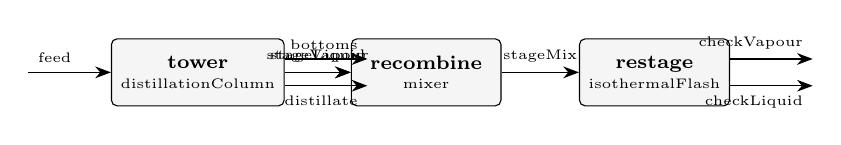
\begin{tikzpicture}[>={Stealth[length=2mm]}, every node/.style={font=\scriptsize}]
  \node[draw, rounded corners=2pt, align=center, minimum width=1.9cm, minimum height=0.85cm, fill=black!4] (tower) at (0.0,-0.0) {\textbf{tower}\\[-1pt]{\tiny distillationColumn}};
  \node[draw, rounded corners=2pt, align=center, minimum width=1.9cm, minimum height=0.85cm, fill=black!4] (recombine) at (2.9,-0.0) {\textbf{recombine}\\[-1pt]{\tiny mixer}};
  \node[draw, rounded corners=2pt, align=center, minimum width=1.9cm, minimum height=0.85cm, fill=black!4] (restage) at (5.8,-0.0) {\textbf{restage}\\[-1pt]{\tiny isothermalFlash}};
  \draw[->] ($(tower.west)+(-1.05,0.00)$) -- ($(tower.west)+(0,0.00)$) node[at start, above, font=\tiny, anchor=south west] {feed};
  \draw[->] (tower) -- (recombine) node[midway, above, font=\tiny] {stageLiquid};
  \draw[->] (tower) -- (recombine) node[midway, above, font=\tiny] {stageVapour};
  \draw[->] (recombine) -- (restage) node[midway, above, font=\tiny] {stageMix};
  \draw[->] ($(tower.east)+(0,-0.17)$) -- ($(tower.east)+(1.05,-0.17)$) node[at end, below, font=\tiny, anchor=north east] {distillate};
  \draw[->] ($(tower.east)+(0,0.17)$) -- ($(tower.east)+(1.05,0.17)$) node[at end, above, font=\tiny, anchor=south east] {bottoms};
  \draw[->] ($(restage.east)+(0,-0.17)$) -- ($(restage.east)+(1.05,-0.17)$) node[at end, below, font=\tiny, anchor=north east] {checkLiquid};
  \draw[->] ($(restage.east)+(0,0.17)$) -- ($(restage.east)+(1.05,0.17)$) node[at end, above, font=\tiny, anchor=south east] {checkVapour};
\end{tikzpicture}
\end{tutscheme}
\tutwhat{The stage identity under CHEMISTRY: a sour-water tray's own two products, recombined and re-flashed, must come back as the same tray}
\begin{tutnarrative}
- Choupo -$\ast$--------------------------------$\ast$ | \textbackslash\{\}|/ C hemicals | Choupo: open-source, glass-box simulation | | \textbackslash\{\}\textbackslash\{\}|// H eat-transfer | Version: Choupo-dev | | \textbackslash\{\}\textbackslash\{\}\textbackslash\{\}|/// O perations | Website: https://choupo.org | | \textbackslash\{\}\textbackslash\{\}|// U nits | Licence: GPL-3.0-or-later | | \textbackslash\{\}|/ P roperties | Tutorial case file -- part of Choupo | | | O ptimization | |

\end{tutnarrative}
\tutreadme{What it demonstrates: a distillation column solved under an aqueous equilibrium, and the proof that the effective K-value it uses per stage is the same equilibrium a flash computes --- checked through two independent code paths, on the apparent components $\ast$and$\ast$ on the ions.}
\tutreadme{Read column12\_stage\_is\_a\_flash first. This is the same construction; only the thermodynamic package differs.}
\tutreadme{Four stages, sour water (NH$_3$ + CO$_2$ in water), 1 atm, R = 2, D = 3 kmol/h. It converges in 7 Newton iterations to ?F? $\approx$ 8e-10, and the profile is the physics:}
\tutreadme{No gammaPhi column can produce that profile, because in a molecular world ammonia's volatility does not depend on how much carbon dioxide has left the liquid. Here it does: the carbon dioxide a liquid still carries is what holds its ammonia as NH$_4$?, so stripping the CO$_2$ sets the ammonia free and the free ammonia then strips. (The usual shorthand for that is "stripping CO$_2$ raises the pH" --- which is true of a fixed solution and is $\ast$not$\ast$ how it reads tray by tray here. See the per-tray table below: it is the carbonate loading that orders cleanly, not the pH.)}
\tutreadme{Both halves of stage 2 are drawn as real streams, recombined, and re-flashed at the same (T, P). Nothing may happen --- and nothing does, to about 1e-9 relative:}
\tutreadme{The ion inventories agreeing is the claim that a comparison of apparent compositions alone would miss: an effective K could reproduce the apparent split while resting on a different chemistry underneath.}
\begin{tutgolden}
\goldrow{stream}{bottoms}{F}{0.0259166666667}
\goldrow{stream}{checkLiquid}{F}{0.00041666666663}
\goldrow{stream}{checkVapour}{F}{0.000138888888925}
\goldrow{stream}{distillate}{F}{0.000833333333333}
\goldrow{stream}{feed}{F}{0.0273055555556}
\goldrow{stream}{stageLiquid}{F}{0.000416666666667}
\goldrow{stream}{stageMix}{F}{0.000555555555556}
\goldrow{stream}{stageVapour}{F}{0.000138888888889}
\goldrow{kpi}{recombine}{F\_out}{0.000555555555556}
\goldrow{kpi}{recombine}{P\_out}{101325}
\goldrow{kpi}{recombine}{T\_out}{483.325341357}
\goldrow{kpi}{recombine}{n\_in}{2}
\goldrow{kpi}{recombine}{vf}{0}
\goldrow{kpi}{restage}{F\_alpha}{0.00041666666663}
\goldmore{31}
\end{tutgolden}

\clearpage
\tutentry{shortcut01\_benzene\_toluene}{tutorials/steady/distillation/shortcut01\_benzene\_toluene}
\begin{tutscheme}
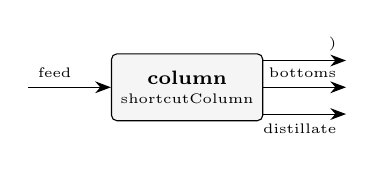
\begin{tikzpicture}[>={Stealth[length=2mm]}, every node/.style={font=\scriptsize}]
  \node[draw, rounded corners=2pt, align=center, minimum width=1.9cm, minimum height=0.85cm, fill=black!4] (column) at (0.0,-0.0) {\textbf{column}\\[-1pt]{\tiny shortcutColumn}};
  \draw[->] ($(column.west)+(-1.05,0.00)$) -- ($(column.west)+(0,0.00)$) node[at start, above, font=\tiny, anchor=south west] {feed};
  \draw[->] ($(column.east)+(0,-0.34)$) -- ($(column.east)+(1.05,-0.34)$) node[at end, below, font=\tiny, anchor=north east] {distillate};
  \draw[->] ($(column.east)+(0,0.00)$) -- ($(column.east)+(1.05,0.00)$) node[at end, above, font=\tiny, anchor=south east] {bottoms};
  \draw[->] ($(column.east)+(0,0.34)$) -- ($(column.east)+(1.05,0.34)$) node[at end, above, font=\tiny, anchor=south east] {)};
\end{tikzpicture}
\end{tutscheme}
\tutwhat{Shortcut (FUG) design of a benzene/toluene column}
\begin{tutnarrative}
- Choupo -$\ast$--------------------------------$\ast$ | \textbackslash\{\}|/ C hemicals | Choupo: open-source, glass-box simulation | | \textbackslash\{\}\textbackslash\{\}|// H eat-transfer | Version: Choupo-dev | | \textbackslash\{\}\textbackslash\{\}\textbackslash\{\}|/// O perations | Website: https://choupo.org | | \textbackslash\{\}\textbackslash\{\}|// U nits | Licence: GPL-3.0-or-later | | \textbackslash\{\}|/ P roperties | Tutorial case file -- part of Choupo | | | O ptimization | |

\end{tutnarrative}
\begin{tutgolden}
\goldrow{stream}{bottoms}{F}{0.0138888888889}
\goldrow{stream}{distillate}{F}{0.0138888888889}
\goldrow{stream}{feed}{F}{0.0277777777778}
\goldrow{kpi}{column}{B}{0.0138888888889}
\goldrow{kpi}{column}{D}{0.0138888888889}
\goldrow{kpi}{column}{N\_min}{10.067785029}
\goldrow{kpi}{column}{N\_theoretical}{21.5880731317}
\goldrow{kpi}{column}{R}{1.68248609289}
\goldrow{kpi}{column}{R\_min}{1.29422007145}
\goldrow{kpi}{column}{alpha\_LK\_HK}{2.49137883567}
\goldrow{kpi}{column}{feed\_stage}{10.7940365659}
\goldrow{kpi}{column}{theta}{1.42716041594}
\goldrow{kpi}{column}{x\_B\_HK}{0.99}
\goldrow{kpi}{column}{x\_D\_LK}{0.99}
\end{tutgolden}

\subsection{drying}
\grouptheory{drying}
\clearpage
\tutentry{evapDryer01\_nacl}{tutorials/steady/drying/evapDryer01\_nacl}
\begin{tutscheme}
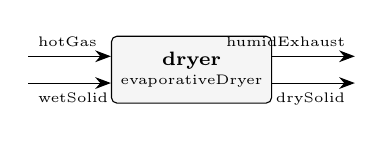
\begin{tikzpicture}[>={Stealth[length=2mm]}, every node/.style={font=\scriptsize}]
  \node[draw, rounded corners=2pt, align=center, minimum width=1.9cm, minimum height=0.85cm, fill=black!4] (dryer) at (0.0,-0.0) {\textbf{dryer}\\[-1pt]{\tiny evaporativeDryer}};
  \draw[->] ($(dryer.west)+(-1.05,-0.17)$) -- ($(dryer.west)+(0,-0.17)$) node[at start, below, font=\tiny, anchor=north west] {wetSolid};
  \draw[->] ($(dryer.west)+(-1.05,0.17)$) -- ($(dryer.west)+(0,0.17)$) node[at start, above, font=\tiny, anchor=south west] {hotGas};
  \draw[->] ($(dryer.east)+(0,-0.17)$) -- ($(dryer.east)+(1.05,-0.17)$) node[at end, below, font=\tiny, anchor=north east] {drySolid};
  \draw[->] ($(dryer.east)+(0,0.17)$) -- ($(dryer.east)+(1.05,0.17)$) node[at end, above, font=\tiny, anchor=south east] {humidExhaust};
\end{tikzpicture}
\end{tutscheme}
\tutwhat{Evaporative dryer: free surface water on NaCl crystals evaporated into dry nitrogen, adiabatic, the binding limit announced}
\begin{tutnarrative}
- Choupo -$\ast$--------------------------------$\ast$ | \textbackslash\{\}|/ C hemicals | Choupo: open-source, glass-box simulation | | | O ptimization | Licence: GPL-3.0-or-later |

\end{tutnarrative}
\begin{tutgolden}
\goldrow{stream}{drySolid}{F}{0.00555555555556}
\goldrow{stream}{hotGas}{F}{0.166805555556}
\goldrow{stream}{humidExhaust}{F}{0.170972222222}
\goldrow{stream}{wetSolid}{F}{0.00972222222222}
\goldrow{kpi}{dryer}{T\_out}{360.675490975}
\goldrow{kpi}{dryer}{X\_final}{0}
\goldrow{kpi}{dryer}{X\_initial}{0.231198665298}
\goldrow{kpi}{dryer}{air\_in\_kmol\_h}{600.5}
\goldrow{kpi}{dryer}{drySolid\_flow}{0.324666666667}
\goldrow{kpi}{dryer}{exhaust\_humidity}{0.0392946211155}
\goldrow{kpi}{dryer}{moisture\_pct\_wb}{0}
\goldrow{kpi}{dryer}{water\_removed}{0.0750625}
\end{tutgolden}

\clearpage
\tutentry{evapDryer02\_energy\_limited}{tutorials/steady/drying/evapDryer02\_energy\_limited}
\begin{tutscheme}
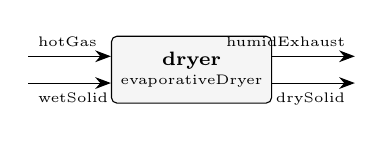
\begin{tikzpicture}[>={Stealth[length=2mm]}, every node/.style={font=\scriptsize}]
  \node[draw, rounded corners=2pt, align=center, minimum width=1.9cm, minimum height=0.85cm, fill=black!4] (dryer) at (0.0,-0.0) {\textbf{dryer}\\[-1pt]{\tiny evaporativeDryer}};
  \draw[->] ($(dryer.west)+(-1.05,-0.17)$) -- ($(dryer.west)+(0,-0.17)$) node[at start, below, font=\tiny, anchor=north west] {wetSolid};
  \draw[->] ($(dryer.west)+(-1.05,0.17)$) -- ($(dryer.west)+(0,0.17)$) node[at start, above, font=\tiny, anchor=south west] {hotGas};
  \draw[->] ($(dryer.east)+(0,-0.17)$) -- ($(dryer.east)+(1.05,-0.17)$) node[at end, below, font=\tiny, anchor=north east] {drySolid};
  \draw[->] ($(dryer.east)+(0,0.17)$) -- ($(dryer.east)+(1.05,0.17)$) node[at end, above, font=\tiny, anchor=south east] {humidExhaust};
\end{tikzpicture}
\end{tutscheme}
\tutwhat{The same dryer starved of gas: 40 kmol/h instead of 600, so the ENERGY floor binds and 16.6 wt\% of the water stays on the crystal}
\begin{tutnarrative}
- Choupo -$\ast$--------------------------------$\ast$ | \textbackslash\{\}|/ C hemicals | Choupo: open-source, glass-box simulation | | | O ptimization | Licence: GPL-3.0-or-later |

\end{tutnarrative}
\begin{tutgolden}
\goldrow{stream}{drySolid}{F}{0.00914216942312}
\goldrow{stream}{hotGas}{F}{0.01125}
\goldrow{stream}{humidExhaust}{F}{0.0118300527991}
\goldrow{stream}{wetSolid}{F}{0.00972222222222}
\goldrow{kpi}{dryer}{T\_out}{310.725305009}
\goldrow{kpi}{dryer}{X\_final}{0.199012881389}
\goldrow{kpi}{dryer}{X\_initial}{0.231198665298}
\goldrow{kpi}{dryer}{air\_in\_kmol\_h}{40.5}
\goldrow{kpi}{dryer}{drySolid\_flow}{0.389279515491}
\goldrow{kpi}{dryer}{exhaust\_humidity}{0.949998302456}
\goldrow{kpi}{dryer}{moisture\_pct\_wb}{16.5980603276}
\goldrow{kpi}{dryer}{water\_removed}{0.0104496511758}
\end{tutgolden}

\clearpage
\tutentry{solidDryer01\_sugar}{tutorials/steady/drying/solidDryer01\_sugar}
\tutwhat{Solid dryer: wet sugar powder dried to sorption equilibrium}
\begin{tutnarrative}
- Choupo -$\ast$--------------------------------$\ast$ | \textbackslash\{\}|/ C hemicals | Choupo: open-source, glass-box simulation | | \textbackslash\{\}\textbackslash\{\}|// H eat-transfer | Version: Choupo-dev | | \textbackslash\{\}\textbackslash\{\}\textbackslash\{\}|/// O perations | Website: https://choupo.org | | \textbackslash\{\}\textbackslash\{\}|// U nits | Licence: GPL-3.0-or-later | | \textbackslash\{\}|/ P roperties | Tutorial case file -- part of Choupo | | | O ptimization | |

\end{tutnarrative}
\begin{tutgolden}
\goldrow{stream}{drySolid}{F}{0.00283583138708}
\goldrow{stream}{hotAir}{F}{0.222222222229}
\goldrow{stream}{humidExhaust}{F}{0.23271974852}
\goldrow{stream}{wetSolid}{F}{0.0133333576778}
\goldrow{kpi}{solidDryer}{T\_out}{347.5126791}
\goldrow{kpi}{solidDryer}{X\_equilibrium}{0.00109945367934}
\goldrow{kpi}{solidDryer}{X\_final}{0.00109945367934}
\goldrow{kpi}{solidDryer}{X\_initial}{0.199991235822}
\goldrow{kpi}{solidDryer}{air\_in\_kmol\_h}{800.000000025}
\goldrow{kpi}{solidDryer}{drySolid\_flow}{0.951878730237}
\goldrow{kpi}{solidDryer}{moisture\_pct\_wb}{0.109824620851}
\goldrow{kpi}{solidDryer}{water\_activity}{0.00431158404412}
\goldrow{kpi}{solidDryer}{water\_removed}{0.189112936127}
\end{tutgolden}

\clearpage
\tutentry{sprayDryer01\_sugar}{tutorials/steady/drying/sprayDryer01\_sugar}
\begin{tutscheme}
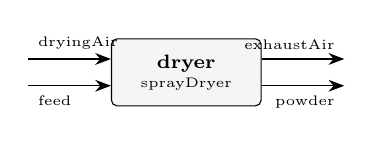
\begin{tikzpicture}[>={Stealth[length=2mm]}, every node/.style={font=\scriptsize}]
  \node[draw, rounded corners=2pt, align=center, minimum width=1.9cm, minimum height=0.85cm, fill=black!4] (dryer) at (0.0,-0.0) {\textbf{dryer}\\[-1pt]{\tiny sprayDryer}};
  \draw[->] ($(dryer.west)+(-1.05,-0.17)$) -- ($(dryer.west)+(0,-0.17)$) node[at start, below, font=\tiny, anchor=north west] {feed};
  \draw[->] ($(dryer.west)+(-1.05,0.17)$) -- ($(dryer.west)+(0,0.17)$) node[at start, above, font=\tiny, anchor=south west] {dryingAir};
  \draw[->] ($(dryer.east)+(0,-0.17)$) -- ($(dryer.east)+(1.05,-0.17)$) node[at end, below, font=\tiny, anchor=north east] {powder};
  \draw[->] ($(dryer.east)+(0,0.17)$) -- ($(dryer.east)+(1.05,0.17)$) node[at end, above, font=\tiny, anchor=south east] {exhaustAir};
\end{tikzpicture}
\end{tutscheme}
\tutwhat{Spray dryer: 40 wt\% sugar solution $\to$ powder (rotary atomiser, Ranz-Marshall)}
\begin{tutnarrative}
- Choupo -$\ast$--------------------------------$\ast$ | \textbackslash\{\}|/ C hemicals | Choupo: open-source, glass-box simulation | | \textbackslash\{\}\textbackslash\{\}|// H eat-transfer | Version: Choupo-dev | | \textbackslash\{\}\textbackslash\{\}\textbackslash\{\}|/// O perations | Website: https://choupo.org | | \textbackslash\{\}\textbackslash\{\}|// U nits | Licence: GPL-3.0-or-later | | \textbackslash\{\}|/ P roperties | Tutorial case file -- part of Choupo | | | O ptimization | |

\end{tutnarrative}
\begin{tutgolden}
\goldrow{stream}{dryingAir}{F}{0.0138888888889}
\goldrow{stream}{exhaustAir}{F}{0.0148058483113}
\goldrow{stream}{feed}{F}{0.000957611111111}
\goldrow{stream}{powder}{F}{4.06516887181e-05}
\goldrow{kpi}{dryer}{Nu}{2.24583682227}
\goldrow{kpi}{dryer}{Pr}{0.746977616919}
\goldrow{kpi}{dryer}{Re}{0.203916784363}
\goldrow{kpi}{dryer}{Sc}{0.6026290984}
\goldrow{kpi}{dryer}{Sh}{2.22885536787}
\goldrow{kpi}{dryer}{T\_out}{372.025243986}
\goldrow{kpi}{dryer}{T\_wetbulb}{318.053221267}
\goldrow{kpi}{dryer}{d\_droplet}{6.04023981348e-05}
\goldrow{kpi}{dryer}{d\_droplet\_micron}{60.4023981348}
\goldrow{kpi}{dryer}{d\_particle}{3.80926671659e-05}
\goldmore{12}
\end{tutgolden}

\clearpage
\tutentry{sprayDryer02\_residence\_sweep}{tutorials/steady/drying/sprayDryer02\_residence\_sweep}
\begin{tutscheme}
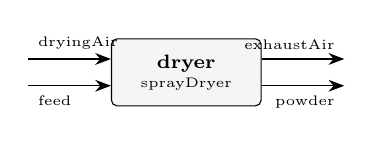
\begin{tikzpicture}[>={Stealth[length=2mm]}, every node/.style={font=\scriptsize}]
  \node[draw, rounded corners=2pt, align=center, minimum width=1.9cm, minimum height=0.85cm, fill=black!4] (dryer) at (0.0,-0.0) {\textbf{dryer}\\[-1pt]{\tiny sprayDryer}};
  \draw[->] ($(dryer.west)+(-1.05,-0.17)$) -- ($(dryer.west)+(0,-0.17)$) node[at start, below, font=\tiny, anchor=north west] {feed};
  \draw[->] ($(dryer.west)+(-1.05,0.17)$) -- ($(dryer.west)+(0,0.17)$) node[at start, above, font=\tiny, anchor=south west] {dryingAir};
  \draw[->] ($(dryer.east)+(0,-0.17)$) -- ($(dryer.east)+(1.05,-0.17)$) node[at end, below, font=\tiny, anchor=north east] {powder};
  \draw[->] ($(dryer.east)+(0,0.17)$) -- ($(dryer.east)+(1.05,0.17)$) node[at end, above, font=\tiny, anchor=south east] {exhaustAir};
\end{tikzpicture}
\end{tutscheme}
\tutwhat{Spray dryer: chamber-height sweep $\to$ the drying curve (residence = L/v; constant + falling rate $\to$ equilibrium)}
\begin{tutnarrative}
- Choupo -$\ast$--------------------------------$\ast$ | \textbackslash\{\}|/ C hemicals | Choupo: open-source, glass-box simulation | | \textbackslash\{\}\textbackslash\{\}|// H eat-transfer | Version: Choupo-dev | | \textbackslash\{\}\textbackslash\{\}\textbackslash\{\}|/// O perations | Website: https://choupo.org | | \textbackslash\{\}\textbackslash\{\}|// U nits | Licence: GPL-3.0-or-later | | \textbackslash\{\}|/ P roperties | Tutorial case file -- part of Choupo | | | O ptimization | |

\end{tutnarrative}

\clearpage
\tutentry{sprayDryer03\_pressure\_nozzle}{tutorials/steady/drying/sprayDryer03\_pressure\_nozzle}
\begin{tutscheme}
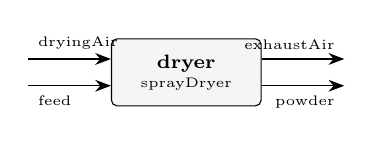
\begin{tikzpicture}[>={Stealth[length=2mm]}, every node/.style={font=\scriptsize}]
  \node[draw, rounded corners=2pt, align=center, minimum width=1.9cm, minimum height=0.85cm, fill=black!4] (dryer) at (0.0,-0.0) {\textbf{dryer}\\[-1pt]{\tiny sprayDryer}};
  \draw[->] ($(dryer.west)+(-1.05,-0.17)$) -- ($(dryer.west)+(0,-0.17)$) node[at start, below, font=\tiny, anchor=north west] {feed};
  \draw[->] ($(dryer.west)+(-1.05,0.17)$) -- ($(dryer.west)+(0,0.17)$) node[at start, above, font=\tiny, anchor=south west] {dryingAir};
  \draw[->] ($(dryer.east)+(0,-0.17)$) -- ($(dryer.east)+(1.05,-0.17)$) node[at end, below, font=\tiny, anchor=north east] {powder};
  \draw[->] ($(dryer.east)+(0,0.17)$) -- ($(dryer.east)+(1.05,0.17)$) node[at end, above, font=\tiny, anchor=south east] {exhaustAir};
\end{tikzpicture}
\end{tutscheme}
\tutwhat{Spray dryer: 40 wt\% sugar solution $\to$ powder (PRESSURE-SWIRL nozzle at 40 bar, d32=9575$\ast$dP\textasciicircum{}-1/3; Ranz-Marshall)}
\begin{tutnarrative}
- Choupo -$\ast$--------------------------------$\ast$ | \textbackslash\{\}|/ C hemicals | Choupo: open-source, glass-box simulation | | \textbackslash\{\}\textbackslash\{\}|// H eat-transfer | Version: Choupo-dev | | \textbackslash\{\}\textbackslash\{\}\textbackslash\{\}|/// O perations | Website: https://choupo.org | | \textbackslash\{\}\textbackslash\{\}|// U nits | Licence: GPL-3.0-or-later | | \textbackslash\{\}|/ P roperties | Tutorial case file -- part of Choupo | | | O ptimization | |

\end{tutnarrative}
\begin{tutgolden}
\goldrow{stream}{dryingAir}{F}{0.0138888888889}
\goldrow{stream}{exhaustAir}{F}{0.0148058483113}
\goldrow{stream}{feed}{F}{0.000957611111111}
\goldrow{stream}{powder}{F}{4.06516887181e-05}
\goldrow{kpi}{dryer}{Nu}{2.24532614778}
\goldrow{kpi}{dryer}{Pr}{0.746977616919}
\goldrow{kpi}{dryer}{Re}{0.203070475508}
\goldrow{kpi}{dryer}{Sc}{0.6026290984}
\goldrow{kpi}{dryer}{Sh}{2.2283799688}
\goldrow{kpi}{dryer}{T\_out}{372.025243986}
\goldrow{kpi}{dryer}{T\_wetbulb}{318.053221267}
\goldrow{kpi}{dryer}{X\_critical}{0.15}
\goldrow{kpi}{dryer}{X\_equilibrium}{0.0132756494842}
\goldrow{kpi}{dryer}{X\_final}{0.0132756494842}
\goldmore{30}
\end{tutgolden}

\clearpage
\tutentry{sprayDryer04\_profiles}{tutorials/steady/drying/sprayDryer04\_profiles}
\begin{tutscheme}
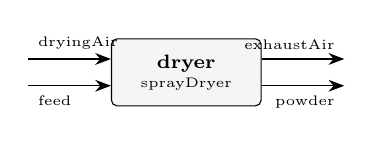
\begin{tikzpicture}[>={Stealth[length=2mm]}, every node/.style={font=\scriptsize}]
  \node[draw, rounded corners=2pt, align=center, minimum width=1.9cm, minimum height=0.85cm, fill=black!4] (dryer) at (0.0,-0.0) {\textbf{dryer}\\[-1pt]{\tiny sprayDryer}};
  \draw[->] ($(dryer.west)+(-1.05,-0.17)$) -- ($(dryer.west)+(0,-0.17)$) node[at start, below, font=\tiny, anchor=north west] {feed};
  \draw[->] ($(dryer.west)+(-1.05,0.17)$) -- ($(dryer.west)+(0,0.17)$) node[at start, above, font=\tiny, anchor=south west] {dryingAir};
  \draw[->] ($(dryer.east)+(0,-0.17)$) -- ($(dryer.east)+(1.05,-0.17)$) node[at end, below, font=\tiny, anchor=north east] {powder};
  \draw[->] ($(dryer.east)+(0,0.17)$) -- ($(dryer.east)+(1.05,0.17)$) node[at end, above, font=\tiny, anchor=south east] {exhaustAir};
\end{tikzpicture}
\end{tutscheme}
\tutwhat{Spray dryer DISTRIBUTED: axial profiles of moisture, size and temperature along the chamber}
\begin{tutnarrative}
- Choupo -$\ast$--------------------------------$\ast$ | \textbackslash\{\}|/ C hemicals | Choupo: open-source, glass-box simulation | | \textbackslash\{\}\textbackslash\{\}|// H eat-transfer | Version: Choupo-dev | | \textbackslash\{\}\textbackslash\{\}\textbackslash\{\}|/// O perations | Website: https://choupo.org | | \textbackslash\{\}\textbackslash\{\}|// U nits | Licence: GPL-3.0-or-later | | \textbackslash\{\}|/ P roperties | Tutorial case file -- part of Choupo | | | O ptimization | |

\end{tutnarrative}
\begin{tutgolden}
\goldrow{stream}{dryingAir}{F}{0.0138888888889}
\goldrow{stream}{exhaustAir}{F}{0.0148058483113}
\goldrow{stream}{feed}{F}{0.000957611111111}
\goldrow{stream}{powder}{F}{4.06516887181e-05}
\goldrow{kpi}{dryer}{Nu}{2.24583682227}
\goldrow{kpi}{dryer}{Pr}{0.746977616919}
\goldrow{kpi}{dryer}{Re}{0.203916784363}
\goldrow{kpi}{dryer}{Sc}{0.6026290984}
\goldrow{kpi}{dryer}{Sh}{2.22885536787}
\goldrow{kpi}{dryer}{T\_out}{372.025243986}
\goldrow{kpi}{dryer}{T\_wetbulb}{318.053221267}
\goldrow{kpi}{dryer}{X\_critical}{0.15}
\goldrow{kpi}{dryer}{X\_equilibrium}{0.0132756494842}
\goldrow{kpi}{dryer}{X\_final}{0.0132756494842}
\goldmore{30}
\end{tutgolden}

\clearpage
\tutentry{sprayDryer05\_whey}{tutorials/steady/drying/sprayDryer05\_whey}
\begin{tutscheme}
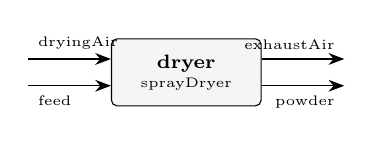
\begin{tikzpicture}[>={Stealth[length=2mm]}, every node/.style={font=\scriptsize}]
  \node[draw, rounded corners=2pt, align=center, minimum width=1.9cm, minimum height=0.85cm, fill=black!4] (dryer) at (0.0,-0.0) {\textbf{dryer}\\[-1pt]{\tiny sprayDryer}};
  \draw[->] ($(dryer.west)+(-1.05,-0.17)$) -- ($(dryer.west)+(0,-0.17)$) node[at start, below, font=\tiny, anchor=north west] {feed};
  \draw[->] ($(dryer.west)+(-1.05,0.17)$) -- ($(dryer.west)+(0,0.17)$) node[at start, above, font=\tiny, anchor=south west] {dryingAir};
  \draw[->] ($(dryer.east)+(0,-0.17)$) -- ($(dryer.east)+(1.05,-0.17)$) node[at end, below, font=\tiny, anchor=north east] {powder};
  \draw[->] ($(dryer.east)+(0,0.17)$) -- ($(dryer.east)+(1.05,0.17)$) node[at end, above, font=\tiny, anchor=south east] {exhaustAir};
\end{tikzpicture}
\end{tutscheme}
\tutwhat{Spray dryer: whey (prob 5.2) -- 500 kg/h, X0=5, rotary co-current, sorption-isotherm residual moisture}
\begin{tutnarrative}
- Choupo -$\ast$--------------------------------$\ast$ | \textbackslash\{\}|/ C hemicals | Choupo: open-source, glass-box simulation | | \textbackslash\{\}\textbackslash\{\}|// H eat-transfer | Version: Choupo-dev | | \textbackslash\{\}\textbackslash\{\}\textbackslash\{\}|/// O perations | Website: https://choupo.org | | \textbackslash\{\}\textbackslash\{\}|// U nits | Licence: GPL-3.0-or-later | | \textbackslash\{\}|/ P roperties | Tutorial case file -- part of Choupo | | | O ptimization | |

\end{tutnarrative}
\begin{tutgolden}
\goldrow{stream}{dryingAir}{F}{0.138888888889}
\goldrow{stream}{exhaustAir}{F}{0.14529654835}
\goldrow{stream}{feed}{F}{0.00649261111111}
\goldrow{stream}{powder}{F}{8.49516499934e-05}
\goldrow{kpi}{dryer}{Nu}{2.33731434528}
\goldrow{kpi}{dryer}{Pr}{0.745230561117}
\goldrow{kpi}{dryer}{Re}{0.384509154435}
\goldrow{kpi}{dryer}{Sc}{0.602916461126}
\goldrow{kpi}{dryer}{Sh}{2.31430911286}
\goldrow{kpi}{dryer}{T\_out}{382.7774359}
\goldrow{kpi}{dryer}{T\_wetbulb}{315.824008236}
\goldrow{kpi}{dryer}{X\_critical}{0.5}
\goldrow{kpi}{dryer}{X\_equilibrium}{0.0134981947613}
\goldrow{kpi}{dryer}{X\_final}{0.0134981947613}
\goldmore{30}
\end{tutgolden}

\clearpage
\tutentry{sprayDryer06\_rea}{tutorials/steady/drying/sprayDryer06\_rea}
\begin{tutscheme}
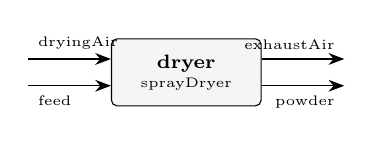
\begin{tikzpicture}[>={Stealth[length=2mm]}, every node/.style={font=\scriptsize}]
  \node[draw, rounded corners=2pt, align=center, minimum width=1.9cm, minimum height=0.85cm, fill=black!4] (dryer) at (0.0,-0.0) {\textbf{dryer}\\[-1pt]{\tiny sprayDryer}};
  \draw[->] ($(dryer.west)+(-1.05,-0.17)$) -- ($(dryer.west)+(0,-0.17)$) node[at start, below, font=\tiny, anchor=north west] {feed};
  \draw[->] ($(dryer.west)+(-1.05,0.17)$) -- ($(dryer.west)+(0,0.17)$) node[at start, above, font=\tiny, anchor=south west] {dryingAir};
  \draw[->] ($(dryer.east)+(0,-0.17)$) -- ($(dryer.east)+(1.05,-0.17)$) node[at end, below, font=\tiny, anchor=north east] {powder};
  \draw[->] ($(dryer.east)+(0,0.17)$) -- ($(dryer.east)+(1.05,0.17)$) node[at end, above, font=\tiny, anchor=south east] {exhaustAir};
\end{tikzpicture}
\end{tutscheme}
\tutwhat{Spray dryer REA (model chen): Reaction Engineering Approach kinetics -- smooth rate, no critical-moisture break}
\begin{tutnarrative}
- Choupo -$\ast$--------------------------------$\ast$ | \textbackslash\{\}|/ C hemicals | Choupo: open-source, glass-box simulation | | \textbackslash\{\}\textbackslash\{\}|// H eat-transfer | Version: Choupo-dev | | \textbackslash\{\}\textbackslash\{\}\textbackslash\{\}|/// O perations | Website: https://choupo.org | | \textbackslash\{\}\textbackslash\{\}|// U nits | Licence: GPL-3.0-or-later | | \textbackslash\{\}|/ P roperties | Tutorial case file -- part of Choupo | | | O ptimization | |

\end{tutnarrative}
\begin{tutgolden}
\goldrow{stream}{dryingAir}{F}{0.0138888888889}
\goldrow{stream}{exhaustAir}{F}{0.0148058483113}
\goldrow{stream}{feed}{F}{0.000957611111111}
\goldrow{stream}{powder}{F}{4.06516887181e-05}
\goldrow{kpi}{dryer}{Nu}{2.24583682227}
\goldrow{kpi}{dryer}{Pr}{0.746977616919}
\goldrow{kpi}{dryer}{Re}{0.203916784363}
\goldrow{kpi}{dryer}{Sc}{0.6026290984}
\goldrow{kpi}{dryer}{Sh}{2.22885536787}
\goldrow{kpi}{dryer}{T\_out}{372.025243986}
\goldrow{kpi}{dryer}{T\_wetbulb}{318.053221267}
\goldrow{kpi}{dryer}{X\_critical}{0.15}
\goldrow{kpi}{dryer}{X\_equilibrium}{0.0132756494842}
\goldrow{kpi}{dryer}{X\_final}{0.0132756494842}
\goldmore{30}
\end{tutgolden}

\clearpage
\tutentry{sprayDryer07\_design}{tutorials/steady/drying/sprayDryer07\_design}
\begin{tutscheme}
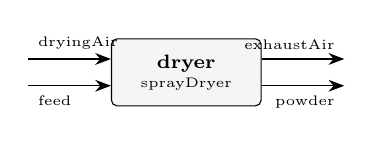
\begin{tikzpicture}[>={Stealth[length=2mm]}, every node/.style={font=\scriptsize}]
  \node[draw, rounded corners=2pt, align=center, minimum width=1.9cm, minimum height=0.85cm, fill=black!4] (dryer) at (0.0,-0.0) {\textbf{dryer}\\[-1pt]{\tiny sprayDryer}};
  \draw[->] ($(dryer.west)+(-1.05,-0.17)$) -- ($(dryer.west)+(0,-0.17)$) node[at start, below, font=\tiny, anchor=north west] {feed};
  \draw[->] ($(dryer.west)+(-1.05,0.17)$) -- ($(dryer.west)+(0,0.17)$) node[at start, above, font=\tiny, anchor=south west] {dryingAir};
  \draw[->] ($(dryer.east)+(0,-0.17)$) -- ($(dryer.east)+(1.05,-0.17)$) node[at end, below, font=\tiny, anchor=north east] {powder};
  \draw[->] ($(dryer.east)+(0,0.17)$) -- ($(dryer.east)+(1.05,0.17)$) node[at end, above, font=\tiny, anchor=south east] {exhaustAir};
\end{tikzpicture}
\end{tutscheme}
\tutwhat{Spray dryer DESIGN: give targets (powder size, residence), the sizing pass inverts to the geometry}
\begin{tutnarrative}
- Choupo -$\ast$--------------------------------$\ast$ | \textbackslash\{\}|/ C hemicals | Choupo: open-source, glass-box simulation | | \textbackslash\{\}\textbackslash\{\}|// H eat-transfer | Version: Choupo-dev | | \textbackslash\{\}\textbackslash\{\}\textbackslash\{\}|/// O perations | Website: https://choupo.org | | \textbackslash\{\}\textbackslash\{\}|// U nits | Licence: GPL-3.0-or-later | | \textbackslash\{\}|/ P roperties | Tutorial case file -- part of Choupo | | | O ptimization | |

\end{tutnarrative}
\begin{tutgolden}
\goldrow{stream}{dryingAir}{F}{0.0138888888889}
\goldrow{stream}{exhaustAir}{F}{0.0148058483113}
\goldrow{stream}{feed}{F}{0.000957611111111}
\goldrow{stream}{powder}{F}{4.06516887181e-05}
\goldrow{kpi}{dryer}{Nu}{2.24583682227}
\goldrow{kpi}{dryer}{Pr}{0.746977616919}
\goldrow{kpi}{dryer}{Re}{0.203916784363}
\goldrow{kpi}{dryer}{Sc}{0.6026290984}
\goldrow{kpi}{dryer}{Sh}{2.22885536787}
\goldrow{kpi}{dryer}{T\_out}{372.025243986}
\goldrow{kpi}{dryer}{T\_wetbulb}{318.053221267}
\goldrow{kpi}{dryer}{X\_critical}{0.15}
\goldrow{kpi}{dryer}{X\_equilibrium}{0.0132756494842}
\goldrow{kpi}{dryer}{X\_final}{0.0132756494842}
\goldmore{31}
\end{tutgolden}

\subsection{economics}
\grouptheory{economics}
\clearpage
\tutentry{economics01\_esterification\_dcf}{tutorials/steady/economics/economics01\_esterification\_dcf}
\begin{tutscheme}
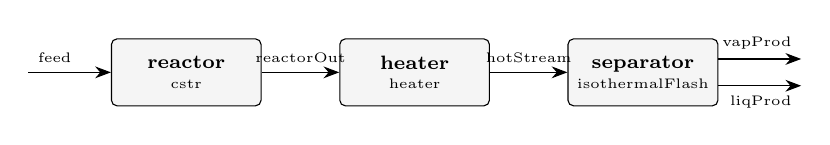
\begin{tikzpicture}[>={Stealth[length=2mm]}, every node/.style={font=\scriptsize}]
  \node[draw, rounded corners=2pt, align=center, minimum width=1.9cm, minimum height=0.85cm, fill=black!4] (reactor) at (0.0,-0.0) {\textbf{reactor}\\[-1pt]{\tiny cstr}};
  \node[draw, rounded corners=2pt, align=center, minimum width=1.9cm, minimum height=0.85cm, fill=black!4] (heater) at (2.9,-0.0) {\textbf{heater}\\[-1pt]{\tiny heater}};
  \node[draw, rounded corners=2pt, align=center, minimum width=1.9cm, minimum height=0.85cm, fill=black!4] (separator) at (5.8,-0.0) {\textbf{separator}\\[-1pt]{\tiny isothermalFlash}};
  \draw[->] ($(reactor.west)+(-1.05,0.00)$) -- ($(reactor.west)+(0,0.00)$) node[at start, above, font=\tiny, anchor=south west] {feed};
  \draw[->] (reactor) -- (heater) node[midway, above, font=\tiny] {reactorOut};
  \draw[->] (heater) -- (separator) node[midway, above, font=\tiny] {hotStream};
  \draw[->] ($(separator.east)+(0,-0.17)$) -- ($(separator.east)+(1.05,-0.17)$) node[at end, below, font=\tiny, anchor=north east] {liqProd};
  \draw[->] ($(separator.east)+(0,0.17)$) -- ($(separator.east)+(1.05,0.17)$) node[at end, above, font=\tiny, anchor=south east] {vapProd};
\end{tikzpicture}
\end{tutscheme}
\tutwhat{Esterification plant: CAPEX (Guthrie) $\to$ OPEX (COM\_d) $\to$ discounted-cash-flow appraisal (NPV/IRR/payback)}
\begin{tutnarrative}
- Choupo -$\ast$--------------------------------$\ast$ | \textbackslash\{\}|/ C hemicals | Choupo: open-source, glass-box simulation | | \textbackslash\{\}\textbackslash\{\}|// H eat-transfer | Version: Choupo-dev | | \textbackslash\{\}\textbackslash\{\}\textbackslash\{\}|/// O perations | Website: https://choupo.org | | \textbackslash\{\}\textbackslash\{\}|// U nits | Licence: GPL-3.0-or-later | | \textbackslash\{\}|/ P roperties | Tutorial case file -- part of Choupo | | | O ptimization | |

\end{tutnarrative}
\tutreadme{A fixed (designed) ethyl-acetate plant taken all the way from equipment sizing to a discounted-cash-flow economic appraisal:}
\tutreadme{1. sizing --- StirredTank for the CSTR, ShellTubeHX for the heater, sized from each unit's KPIs. 2. costing --- Guthrie/Turton purchased + bare-module + total-module cost, CEPCI-updated to the target year, in EUR. 3. economics --- the new EconomicsPass: it builds the CAPEX ladder (FCI, working capital, TCI), the Turton cost-of-manufacture COM\_d, revenue, a straight-line-depreciation cash-flow timeline, then NPV, IRR (bisection bracket + Newton polish), and discounted + simple payback.}
\tutreadme{Every cost factor and DCF assumption is dict-owned and printed --- read the appraisal block and you can re-derive every number by hand.}
\tutreadme{Depreciation enters the DCF exactly once (it is $\ast$not$\ast$ in COM\_d) --- the classic textbook double-count is avoided. Working capital is an outflow at startup and is recovered untaxed at end-of-life.}
\tutreadme{Market/time-specific data --- product and feed prices, labour rate, FX --- lives only in constant/economics, each value dated and primary-cited (an index/bulletin/agency named in a provenance\{\} block). The EconomicsPass refuses to run if a required price is absent, with a remedy message; set economics.refuseOnMissingPrice 0; in the postDict to switch to defaulted-but-loud. No price ever defaults to a literal in code.}
\tutreadme{The economics pass also publishes its headline scalars into result.kpis["economics"] (IRR, NPV, paybackYears, FCI, TCI, COM\_d), which is what lets a sweep or optimisation read economics as an ordinary response --- see economics02\_irr\_sweep.}

\clearpage
\tutentry{economics02\_irr\_sweep}{tutorials/steady/economics/economics02\_irr\_sweep}
\begin{tutscheme}
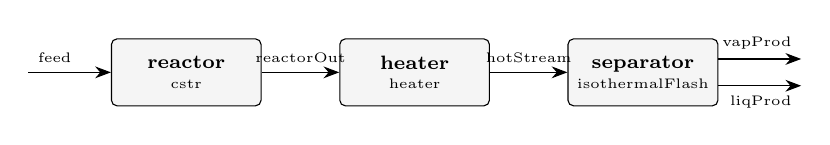
\begin{tikzpicture}[>={Stealth[length=2mm]}, every node/.style={font=\scriptsize}]
  \node[draw, rounded corners=2pt, align=center, minimum width=1.9cm, minimum height=0.85cm, fill=black!4] (reactor) at (0.0,-0.0) {\textbf{reactor}\\[-1pt]{\tiny cstr}};
  \node[draw, rounded corners=2pt, align=center, minimum width=1.9cm, minimum height=0.85cm, fill=black!4] (heater) at (2.9,-0.0) {\textbf{heater}\\[-1pt]{\tiny heater}};
  \node[draw, rounded corners=2pt, align=center, minimum width=1.9cm, minimum height=0.85cm, fill=black!4] (separator) at (5.8,-0.0) {\textbf{separator}\\[-1pt]{\tiny isothermalFlash}};
  \draw[->] ($(reactor.west)+(-1.05,0.00)$) -- ($(reactor.west)+(0,0.00)$) node[at start, above, font=\tiny, anchor=south west] {feed};
  \draw[->] (reactor) -- (heater) node[midway, above, font=\tiny] {reactorOut};
  \draw[->] (heater) -- (separator) node[midway, above, font=\tiny] {hotStream};
  \draw[->] ($(separator.east)+(0,-0.17)$) -- ($(separator.east)+(1.05,-0.17)$) node[at end, below, font=\tiny, anchor=north east] {liqProd};
  \draw[->] ($(separator.east)+(0,0.17)$) -- ($(separator.east)+(1.05,0.17)$) node[at end, above, font=\tiny, anchor=south east] {vapProd};
\end{tikzpicture}
\end{tutscheme}
\tutwhat{Sweep reactor volume; read economics.IRR/NPV/payback per point (SweepDriver runs the post chain)}
\begin{tutnarrative}
- Choupo -$\ast$--------------------------------$\ast$ | \textbackslash\{\}|/ C hemicals | Choupo: open-source, glass-box simulation | | \textbackslash\{\}\textbackslash\{\}|// H eat-transfer | Version: Choupo-dev | | \textbackslash\{\}\textbackslash\{\}\textbackslash\{\}|/// O perations | Website: https://choupo.org | | \textbackslash\{\}\textbackslash\{\}|// U nits | Licence: GPL-3.0-or-later | | \textbackslash\{\}|/ P roperties | Tutorial case file -- part of Choupo | | | O ptimization | |

\end{tutnarrative}
\tutreadme{The same esterification plant as economics01, but driven by a sensitivity sweep over the reactor volume that reads economic responses at every point:}
\tutreadme{The SweepDriver now runs the full post-processing chain (sizing $\to$ costing $\to$ economics) on each converged point, so the headline economic scalars the EconomicsPass publishes into result.kpis["economics"] resolve as ordinary unit.kpi responses. A sweep can finally $\ast$see cost$\ast$:}
\tutreadme{A bigger reactor raises conversion (more product, more revenue) but raises CAPEX and feed throughput --- the IRR falls monotonically over this range, a trade-off invisible from a single CAPEX number.}
\tutreadme{> The range floors at 4 m$^3$ on purpose: below \textasciitilde{}3 m$^3$ the lower conversion > drops the mixture bubble point and the fixed-duty heater would cross the > saturation dome (a heater is sensible-only) --- the deliberate validity edge.}

\subsection{evaporation}
\grouptheory{evaporation}
\clearpage
\tutentry{evaporator01\_brine}{tutorials/steady/evaporation/evaporator01\_brine}
\begin{tutscheme}
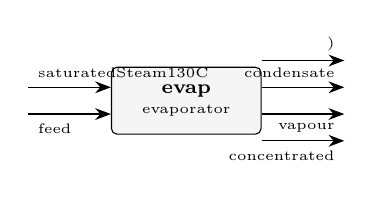
\begin{tikzpicture}[>={Stealth[length=2mm]}, every node/.style={font=\scriptsize}]
  \node[draw, rounded corners=2pt, align=center, minimum width=1.9cm, minimum height=0.85cm, fill=black!4] (evap) at (0.0,-0.0) {\textbf{evap}\\[-1pt]{\tiny evaporator}};
  \draw[->] ($(evap.west)+(-1.05,-0.17)$) -- ($(evap.west)+(0,-0.17)$) node[at start, below, font=\tiny, anchor=north west] {feed};
  \draw[->] ($(evap.west)+(-1.05,0.17)$) -- ($(evap.west)+(0,0.17)$) node[at start, above, font=\tiny, anchor=south west] {saturatedSteam130C};
  \draw[->] ($(evap.east)+(0,-0.51)$) -- ($(evap.east)+(1.05,-0.51)$) node[at end, below, font=\tiny, anchor=north east] {concentrated};
  \draw[->] ($(evap.east)+(0,-0.17)$) -- ($(evap.east)+(1.05,-0.17)$) node[at end, below, font=\tiny, anchor=north east] {vapour};
  \draw[->] ($(evap.east)+(0,0.17)$) -- ($(evap.east)+(1.05,0.17)$) node[at end, above, font=\tiny, anchor=south east] {condensate};
  \draw[->] ($(evap.east)+(0,0.51)$) -- ($(evap.east)+(1.05,0.51)$) node[at end, above, font=\tiny, anchor=south east] {)};
\end{tikzpicture}
\end{tutscheme}
\tutwhat{Single-effect evaporator: 35 g/L brine at 1 bar; the fixed steam duty/UA evaporates \textasciitilde{}82 \% of the feed water (V/F=0.82), enriching NaCl \textasciitilde{}5.5x (x 0.011 $\to$ 0.059) -- duty-driven, not a target (BPE included)}
\begin{tutnarrative}
- Choupo -$\ast$--------------------------------$\ast$ | \textbackslash\{\}|/ C hemicals | Choupo: open-source, glass-box simulation | | \textbackslash\{\}\textbackslash\{\}|// H eat-transfer | Version: Choupo-dev | | \textbackslash\{\}\textbackslash\{\}\textbackslash\{\}|/// O perations | Website: https://choupo.org | | \textbackslash\{\}\textbackslash\{\}|// U nits | Licence: GPL-3.0-or-later | | \textbackslash\{\}|/ P roperties | Tutorial case file -- part of Choupo | | | O ptimization | |

\end{tutnarrative}
\begin{tutgolden}
\goldrow{stream}{concentrated}{F}{0.00498887089392}
\goldrow{stream}{condensate}{F}{0.0277777777778}
\goldrow{stream}{feed}{F}{0.0277777777778}
\goldrow{stream}{saturatedSteam130C}{F}{0.0277777777778}
\goldrow{stream}{vapour}{F}{0.0227889068839}
\goldrow{kpi}{evap}{A}{20}
\goldrow{kpi}{evap}{A\_m2}{20}
\goldrow{kpi}{evap}{BPE}{1.79842779271}
\goldrow{kpi}{evap}{F\_conc}{0.00498887089392}
\goldrow{kpi}{evap}{F\_conc\_kmol\_h}{17.9599352181}
\goldrow{kpi}{evap}{F\_conc\_mass}{0.101856029987}
\goldrow{kpi}{evap}{F\_cond}{0.500416666667}
\goldrow{kpi}{evap}{F\_cond\_kg\_h}{1801.5}
\goldrow{kpi}{evap}{F\_in}{0.0277777777778}
\goldmore{19}
\end{tutgolden}

\clearpage
\tutentry{evaporator02\_triple\_effect\_sugar}{tutorials/steady/evaporation/evaporator02\_triple\_effect\_sugar}
\begin{tutscheme}
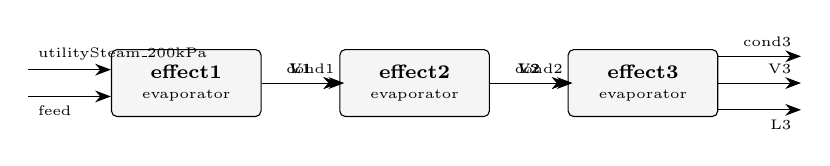
\begin{tikzpicture}[>={Stealth[length=2mm]}, every node/.style={font=\scriptsize}]
  \node[draw, rounded corners=2pt, align=center, minimum width=1.9cm, minimum height=0.85cm, fill=black!4] (effect1) at (0.0,-0.0) {\textbf{effect1}\\[-1pt]{\tiny evaporator}};
  \node[draw, rounded corners=2pt, align=center, minimum width=1.9cm, minimum height=0.85cm, fill=black!4] (effect2) at (2.9,-0.0) {\textbf{effect2}\\[-1pt]{\tiny evaporator}};
  \node[draw, rounded corners=2pt, align=center, minimum width=1.9cm, minimum height=0.85cm, fill=black!4] (effect3) at (5.8,-0.0) {\textbf{effect3}\\[-1pt]{\tiny evaporator}};
  \draw[->] ($(effect1.west)+(-1.05,-0.17)$) -- ($(effect1.west)+(0,-0.17)$) node[at start, below, font=\tiny, anchor=north west] {feed};
  \draw[->] ($(effect1.west)+(-1.05,0.17)$) -- ($(effect1.west)+(0,0.17)$) node[at start, above, font=\tiny, anchor=south west] {utilitySteam\_200kPa};
  \draw[->] (effect1) -- (effect2) node[midway, above, font=\tiny] {L1};
  \draw[->] (effect1) -- (effect2) node[midway, above, font=\tiny] {V1};
  \draw[->] (effect2) -- (effect3) node[midway, above, font=\tiny] {L2};
  \draw[->] (effect2) -- (effect3) node[midway, above, font=\tiny] {V2};
  \draw[->] ($(effect1.east)+(0,0.00)$) -- ($(effect1.east)+(1.05,0.00)$) node[at end, above, font=\tiny, anchor=south east] {cond1};
  \draw[->] ($(effect2.east)+(0,0.00)$) -- ($(effect2.east)+(1.05,0.00)$) node[at end, above, font=\tiny, anchor=south east] {cond2};
  \draw[->] ($(effect3.east)+(0,-0.34)$) -- ($(effect3.east)+(1.05,-0.34)$) node[at end, below, font=\tiny, anchor=north east] {L3};
  \draw[->] ($(effect3.east)+(0,0.00)$) -- ($(effect3.east)+(1.05,0.00)$) node[at end, above, font=\tiny, anchor=south east] {V3};
  \draw[->] ($(effect3.east)+(0,0.34)$) -- ($(effect3.east)+(1.05,0.34)$) node[at end, above, font=\tiny, anchor=south east] {cond3};
\end{tikzpicture}
\end{tutscheme}
\tutwhat{Triple-effect cocurrent evaporator: 22500 kg/h sugar solution 5\%$\to$25\% (textbook Example 10.4)}
\begin{tutnarrative}
- Choupo -$\ast$--------------------------------$\ast$ | \textbackslash\{\}|/ C hemicals | Choupo: open-source, glass-box simulation | | \textbackslash\{\}\textbackslash\{\}|// H eat-transfer | Version: Choupo-dev | | \textbackslash\{\}\textbackslash\{\}\textbackslash\{\}|/// O perations | Website: https://choupo.org | | \textbackslash\{\}\textbackslash\{\}|// U nits | Licence: GPL-3.0-or-later | | \textbackslash\{\}|/ P roperties | Tutorial case file -- part of Choupo | | | O ptimization | |

\end{tutnarrative}
\begin{tutgolden}
\goldrow{stream}{L1}{F}{0.243400997575}
\goldrow{stream}{L2}{F}{0.150822370746}
\goldrow{stream}{L3}{F}{0.0533879418767}
\goldrow{stream}{V1}{F}{0.0870984081237}
\goldrow{stream}{V2}{F}{0.0925786268285}
\goldrow{stream}{V3}{F}{0.0974344288697}
\goldrow{stream}{cond1}{F}{0.1375}
\goldrow{stream}{cond2}{F}{0.0870984081237}
\goldrow{stream}{cond3}{F}{0.0925786268285}
\goldrow{stream}{feed}{F}{0.330499405699}
\goldrow{stream}{utilitySteam\_200kPa}{F}{0.1375}
\goldrow{kpi}{effect1}{A}{100}
\goldrow{kpi}{effect1}{A\_m2}{100}
\goldrow{kpi}{effect1}{BPE}{0.107198891506}
\goldmore{81}
\end{tutgolden}

\clearpage
\tutentry{evaporator03\_co\_current}{tutorials/steady/evaporation/evaporator03\_co\_current}
\begin{tutscheme}
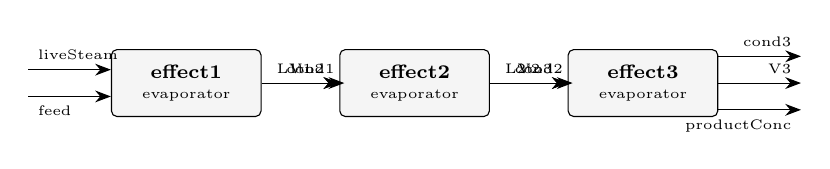
\begin{tikzpicture}[>={Stealth[length=2mm]}, every node/.style={font=\scriptsize}]
  \node[draw, rounded corners=2pt, align=center, minimum width=1.9cm, minimum height=0.85cm, fill=black!4] (effect1) at (0.0,-0.0) {\textbf{effect1}\\[-1pt]{\tiny evaporator}};
  \node[draw, rounded corners=2pt, align=center, minimum width=1.9cm, minimum height=0.85cm, fill=black!4] (effect2) at (2.9,-0.0) {\textbf{effect2}\\[-1pt]{\tiny evaporator}};
  \node[draw, rounded corners=2pt, align=center, minimum width=1.9cm, minimum height=0.85cm, fill=black!4] (effect3) at (5.8,-0.0) {\textbf{effect3}\\[-1pt]{\tiny evaporator}};
  \draw[->] ($(effect1.west)+(-1.05,-0.17)$) -- ($(effect1.west)+(0,-0.17)$) node[at start, below, font=\tiny, anchor=north west] {feed};
  \draw[->] ($(effect1.west)+(-1.05,0.17)$) -- ($(effect1.west)+(0,0.17)$) node[at start, above, font=\tiny, anchor=south west] {liveSteam};
  \draw[->] (effect1) -- (effect2) node[midway, above, font=\tiny] {L1to2};
  \draw[->] (effect1) -- (effect2) node[midway, above, font=\tiny] {V1};
  \draw[->] (effect2) -- (effect3) node[midway, above, font=\tiny] {L2to3};
  \draw[->] (effect2) -- (effect3) node[midway, above, font=\tiny] {V2};
  \draw[->] ($(effect1.east)+(0,0.00)$) -- ($(effect1.east)+(1.05,0.00)$) node[at end, above, font=\tiny, anchor=south east] {cond1};
  \draw[->] ($(effect2.east)+(0,0.00)$) -- ($(effect2.east)+(1.05,0.00)$) node[at end, above, font=\tiny, anchor=south east] {cond2};
  \draw[->] ($(effect3.east)+(0,-0.34)$) -- ($(effect3.east)+(1.05,-0.34)$) node[at end, below, font=\tiny, anchor=north east] {productConc};
  \draw[->] ($(effect3.east)+(0,0.00)$) -- ($(effect3.east)+(1.05,0.00)$) node[at end, above, font=\tiny, anchor=south east] {V3};
  \draw[->] ($(effect3.east)+(0,0.34)$) -- ($(effect3.east)+(1.05,0.34)$) node[at end, above, font=\tiny, anchor=south east] {cond3};
\end{tikzpicture}
\end{tutscheme}
\tutwhat{Co-current forward-feed triple-effect evaporator, user-defined components (textbook problem 10.38, case a)}
\begin{tutnarrative}
- Choupo -$\ast$--------------------------------$\ast$ | \textbackslash\{\}|/ C hemicals | Choupo: open-source, glass-box simulation | | \textbackslash\{\}\textbackslash\{\}|// H eat-transfer | Version: Choupo-dev | | \textbackslash\{\}\textbackslash\{\}\textbackslash\{\}|/// O perations | Website: https://choupo.org | | \textbackslash\{\}\textbackslash\{\}|// U nits | Licence: GPL-3.0-or-later | | \textbackslash\{\}|/ P roperties | Tutorial case file -- part of Choupo | | | O ptimization | |

\end{tutnarrative}
\begin{tutgolden}
\goldrow{stream}{L1to2}{F}{0.0469536109199}
\goldrow{stream}{L2to3}{F}{0.0295647943065}
\goldrow{stream}{V1}{F}{0.0161887935578}
\goldrow{stream}{V2}{F}{0.0173888166134}
\goldrow{stream}{V3}{F}{0.018462595509}
\goldrow{stream}{cond1}{F}{0.0262363636123}
\goldrow{stream}{cond2}{F}{0.0161887935578}
\goldrow{stream}{cond3}{F}{0.0173888166134}
\goldrow{stream}{feed}{F}{0.0631424044778}
\goldrow{stream}{liveSteam}{F}{0.0262363636123}
\goldrow{stream}{productConc}{F}{0.0111021987975}
\goldrow{kpi}{effect1}{A}{16.5383245281}
\goldrow{kpi}{effect1}{A\_m2}{16.5383245281}
\goldrow{kpi}{effect1}{BPE}{0}
\goldmore{81}
\end{tutgolden}

\clearpage
\tutentry{evaporator04\_orange\_juice\_simple}{tutorials/steady/evaporation/evaporator04\_orange\_juice\_simple}
\begin{tutscheme}
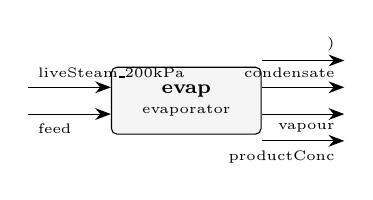
\begin{tikzpicture}[>={Stealth[length=2mm]}, every node/.style={font=\scriptsize}]
  \node[draw, rounded corners=2pt, align=center, minimum width=1.9cm, minimum height=0.85cm, fill=black!4] (evap) at (0.0,-0.0) {\textbf{evap}\\[-1pt]{\tiny evaporator}};
  \draw[->] ($(evap.west)+(-1.05,-0.17)$) -- ($(evap.west)+(0,-0.17)$) node[at start, below, font=\tiny, anchor=north west] {feed};
  \draw[->] ($(evap.west)+(-1.05,0.17)$) -- ($(evap.west)+(0,0.17)$) node[at start, above, font=\tiny, anchor=south west] {liveSteam\_200kPa};
  \draw[->] ($(evap.east)+(0,-0.51)$) -- ($(evap.east)+(1.05,-0.51)$) node[at end, below, font=\tiny, anchor=north east] {productConc};
  \draw[->] ($(evap.east)+(0,-0.17)$) -- ($(evap.east)+(1.05,-0.17)$) node[at end, below, font=\tiny, anchor=north east] {vapour};
  \draw[->] ($(evap.east)+(0,0.17)$) -- ($(evap.east)+(1.05,0.17)$) node[at end, above, font=\tiny, anchor=south east] {condensate};
  \draw[->] ($(evap.east)+(0,0.51)$) -- ($(evap.east)+(1.05,0.51)$) node[at end, above, font=\tiny, anchor=south east] {)};
\end{tikzpicture}
\end{tutscheme}
\tutwhat{Single-effect evaporator concentrating orange juice 10\% to 50\% solids (textbook Example 10.2 a-c, without BPE)}
\begin{tutnarrative}
- Choupo -$\ast$--------------------------------$\ast$ | \textbackslash\{\}|/ C hemicals | Choupo: open-source, glass-box simulation | | \textbackslash\{\}\textbackslash\{\}|// H eat-transfer | Version: Choupo-dev | | \textbackslash\{\}\textbackslash\{\}\textbackslash\{\}|/// O perations | Website: https://choupo.org | | \textbackslash\{\}\textbackslash\{\}|// U nits | Licence: GPL-3.0-or-later | | \textbackslash\{\}|/ P roperties | Tutorial case file -- part of Choupo | | | O ptimization | |

\end{tutnarrative}
\begin{tutgolden}
\goldrow{stream}{condensate}{F}{0.360686102898}
\goldrow{stream}{feed}{F}{0.350791135988}
\goldrow{stream}{liveSteam\_200kPa}{F}{0.360686102898}
\goldrow{stream}{productConc}{F}{0.0424059629635}
\goldrow{stream}{vapour}{F}{0.308385173024}
\goldrow{kpi}{evap}{A}{75.5133330137}
\goldrow{kpi}{evap}{A\_m2}{75.5133330137}
\goldrow{kpi}{evap}{BPE}{0}
\goldrow{kpi}{evap}{F\_conc}{0.0424059629635}
\goldrow{kpi}{evap}{F\_conc\_kmol\_h}{152.661466669}
\goldrow{kpi}{evap}{F\_conc\_mass}{1.38888555242}
\goldrow{kpi}{evap}{F\_cond}{6.49776014371}
\goldrow{kpi}{evap}{F\_cond\_kg\_h}{23391.9365174}
\goldrow{kpi}{evap}{F\_in}{0.350791135988}
\goldmore{19}
\end{tutgolden}

\clearpage
\tutentry{evaporator05\_counter\_current}{tutorials/steady/evaporation/evaporator05\_counter\_current}
\begin{tutscheme}
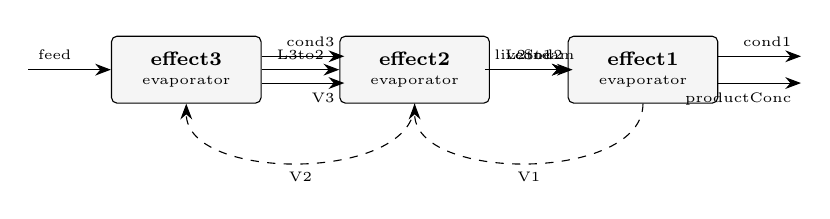
\begin{tikzpicture}[>={Stealth[length=2mm]}, every node/.style={font=\scriptsize}]
  \node[draw, rounded corners=2pt, align=center, minimum width=1.9cm, minimum height=0.85cm, fill=black!4] (effect3) at (20.3,-0.0) {\textbf{effect3}\\[-1pt]{\tiny evaporator}};
  \node[draw, rounded corners=2pt, align=center, minimum width=1.9cm, minimum height=0.85cm, fill=black!4] (effect2) at (23.2,-0.0) {\textbf{effect2}\\[-1pt]{\tiny evaporator}};
  \node[draw, rounded corners=2pt, align=center, minimum width=1.9cm, minimum height=0.85cm, fill=black!4] (effect1) at (26.1,-0.0) {\textbf{effect1}\\[-1pt]{\tiny evaporator}};
  \draw[->] ($(effect3.west)+(-1.05,0.00)$) -- ($(effect3.west)+(0,0.00)$) node[at start, above, font=\tiny, anchor=south west] {feed};
  \draw[->, dashed] (effect2.south) .. controls +(0,-1.0) and +(0,-1.0) .. (effect3.south) node[midway, below, font=\tiny] {V2};
  \draw[->] (effect3) -- (effect2) node[midway, above, font=\tiny] {L3to2};
  \draw[->, dashed] (effect1.south) .. controls +(0,-1.0) and +(0,-1.0) .. (effect2.south) node[midway, below, font=\tiny] {V1};
  \draw[->] (effect2) -- (effect1) node[midway, above, font=\tiny] {L2to1};
  \draw[->] ($(effect1.west)+(-1.05,0.00)$) -- ($(effect1.west)+(0,0.00)$) node[at start, above, font=\tiny, anchor=south west] {liveSteam};
  \draw[->] ($(effect3.east)+(0,-0.17)$) -- ($(effect3.east)+(1.05,-0.17)$) node[at end, below, font=\tiny, anchor=north east] {V3};
  \draw[->] ($(effect3.east)+(0,0.17)$) -- ($(effect3.east)+(1.05,0.17)$) node[at end, above, font=\tiny, anchor=south east] {cond3};
  \draw[->] ($(effect2.east)+(0,0.00)$) -- ($(effect2.east)+(1.05,0.00)$) node[at end, above, font=\tiny, anchor=south east] {cond2};
  \draw[->] ($(effect1.east)+(0,-0.17)$) -- ($(effect1.east)+(1.05,-0.17)$) node[at end, below, font=\tiny, anchor=north east] {productConc};
  \draw[->] ($(effect1.east)+(0,0.17)$) -- ($(effect1.east)+(1.05,0.17)$) node[at end, above, font=\tiny, anchor=south east] {cond1};
\end{tikzpicture}
\end{tutscheme}
\tutwhat{Counter-current backward-feed triple-effect evaporator (textbook problem 10.38 variant)}
\begin{tutnarrative}
- Choupo -$\ast$--------------------------------$\ast$ | \textbackslash\{\}|/ C hemicals | Choupo: open-source, glass-box simulation | | \textbackslash\{\}\textbackslash\{\}|// H eat-transfer | Version: Choupo-dev | | \textbackslash\{\}\textbackslash\{\}\textbackslash\{\}|/// O perations | Website: https://choupo.org | | \textbackslash\{\}\textbackslash\{\}|// U nits | Licence: GPL-3.0-or-later | | \textbackslash\{\}|/ P roperties | Tutorial case file -- part of Choupo | | | O ptimization | |

\end{tutnarrative}
\begin{tutgolden}
\goldrow{stream}{L2to1}{F}{0.0319496046345}
\goldrow{stream}{L3to2}{F}{0.0496904316429}
\goldrow{stream}{V1}{F}{0.020847035226}
\goldrow{stream}{V2}{F}{0.0177408270084}
\goldrow{stream}{V3}{F}{0.0134519728349}
\goldrow{stream}{cond1}{F}{0.0227907734916}
\goldrow{stream}{cond2}{F}{0.0208470355984}
\goldrow{stream}{cond3}{F}{0.0177408244446}
\goldrow{stream}{feed}{F}{0.0631424044778}
\goldrow{stream}{liveSteam}{F}{0.0227907734916}
\goldrow{stream}{productConc}{F}{0.0111025694085}
\goldrow{kpi}{effect1}{A}{17.1719452001}
\goldrow{kpi}{effect1}{A\_m2}{17.1719452001}
\goldrow{kpi}{effect1}{BPE}{0}
\goldmore{81}
\end{tutgolden}

\clearpage
\tutentry{evaporator06\_nacl\_pitzer}{tutorials/steady/evaporation/evaporator06\_nacl\_pitzer}
\begin{tutscheme}
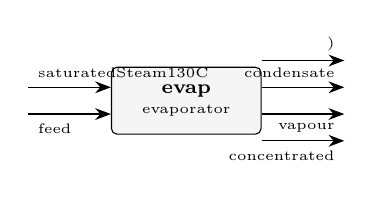
\begin{tikzpicture}[>={Stealth[length=2mm]}, every node/.style={font=\scriptsize}]
  \node[draw, rounded corners=2pt, align=center, minimum width=1.9cm, minimum height=0.85cm, fill=black!4] (evap) at (0.0,-0.0) {\textbf{evap}\\[-1pt]{\tiny evaporator}};
  \draw[->] ($(evap.west)+(-1.05,-0.17)$) -- ($(evap.west)+(0,-0.17)$) node[at start, below, font=\tiny, anchor=north west] {feed};
  \draw[->] ($(evap.west)+(-1.05,0.17)$) -- ($(evap.west)+(0,0.17)$) node[at start, above, font=\tiny, anchor=south west] {saturatedSteam130C};
  \draw[->] ($(evap.east)+(0,-0.51)$) -- ($(evap.east)+(1.05,-0.51)$) node[at end, below, font=\tiny, anchor=north east] {concentrated};
  \draw[->] ($(evap.east)+(0,-0.17)$) -- ($(evap.east)+(1.05,-0.17)$) node[at end, below, font=\tiny, anchor=north east] {vapour};
  \draw[->] ($(evap.east)+(0,0.17)$) -- ($(evap.east)+(1.05,0.17)$) node[at end, above, font=\tiny, anchor=south east] {condensate};
  \draw[->] ($(evap.east)+(0,0.51)$) -- ($(evap.east)+(1.05,0.51)$) node[at end, above, font=\tiny, anchor=south east] {)};
\end{tikzpicture}
\end{tutscheme}
\tutwhat{Single-effect NaCl evaporator with the boiling-point elevation from the PITZER electrolyte model (a\_w), not the ideal K\_b$\ast$m. Concentrated brine $\to$ BPE several degrees, the real value.}
\begin{tutnarrative}
- Choupo -$\ast$--------------------------------$\ast$ | \textbackslash\{\}|/ C hemicals | Choupo: open-source, glass-box simulation | | \textbackslash\{\}\textbackslash\{\}|// H eat-transfer | Version: Choupo-dev | | \textbackslash\{\}\textbackslash\{\}\textbackslash\{\}|/// O perations | Website: https://choupo.org | | \textbackslash\{\}\textbackslash\{\}|// U nits | Licence: GPL-3.0-or-later | | \textbackslash\{\}|/ P roperties | Tutorial case file -- part of Choupo | | | O ptimization | |

\end{tutnarrative}
\begin{tutgolden}
\goldrow{stream}{concentrated}{F}{0.0203403273098}
\goldrow{stream}{condensate}{F}{0.0125}
\goldrow{stream}{feed}{F}{0.0277777777778}
\goldrow{stream}{saturatedSteam130C}{F}{0.0125}
\goldrow{stream}{vapour}{F}{0.00743745046799}
\goldrow{kpi}{evap}{A}{20}
\goldrow{kpi}{evap}{A\_m2}{20}
\goldrow{kpi}{evap}{BPE}{5.06216808829}
\goldrow{kpi}{evap}{F\_conc}{0.0203403273098}
\goldrow{kpi}{evap}{F\_conc\_kmol\_h}{73.2251783152}
\goldrow{kpi}{evap}{F\_conc\_mass}{0.422576829819}
\goldrow{kpi}{evap}{F\_cond}{0.2251875}
\goldrow{kpi}{evap}{F\_cond\_kg\_h}{810.675}
\goldrow{kpi}{evap}{F\_in}{0.0277777777778}
\goldmore{19}
\end{tutgolden}

\clearpage
\tutentry{evaporator07\_nacl\_enrtl}{tutorials/steady/evaporation/evaporator07\_nacl\_enrtl}
\begin{tutscheme}
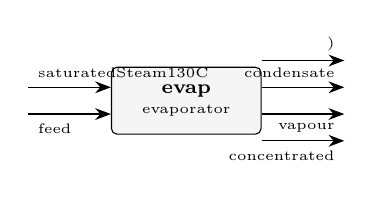
\begin{tikzpicture}[>={Stealth[length=2mm]}, every node/.style={font=\scriptsize}]
  \node[draw, rounded corners=2pt, align=center, minimum width=1.9cm, minimum height=0.85cm, fill=black!4] (evap) at (0.0,-0.0) {\textbf{evap}\\[-1pt]{\tiny evaporator}};
  \draw[->] ($(evap.west)+(-1.05,-0.17)$) -- ($(evap.west)+(0,-0.17)$) node[at start, below, font=\tiny, anchor=north west] {feed};
  \draw[->] ($(evap.west)+(-1.05,0.17)$) -- ($(evap.west)+(0,0.17)$) node[at start, above, font=\tiny, anchor=south west] {saturatedSteam130C};
  \draw[->] ($(evap.east)+(0,-0.51)$) -- ($(evap.east)+(1.05,-0.51)$) node[at end, below, font=\tiny, anchor=north east] {concentrated};
  \draw[->] ($(evap.east)+(0,-0.17)$) -- ($(evap.east)+(1.05,-0.17)$) node[at end, below, font=\tiny, anchor=north east] {vapour};
  \draw[->] ($(evap.east)+(0,0.17)$) -- ($(evap.east)+(1.05,0.17)$) node[at end, above, font=\tiny, anchor=south east] {condensate};
  \draw[->] ($(evap.east)+(0,0.51)$) -- ($(evap.east)+(1.05,0.51)$) node[at end, above, font=\tiny, anchor=south east] {)};
\end{tikzpicture}
\end{tutscheme}
\tutwhat{Single-effect NaCl evaporator with the boiling-point elevation from the eNRTL water activity (electrolyte-NRTL) -- the same slot as model pitzer, one word changed. eNRTL is the model for salt in a non-ideal molecular solvent.}
\begin{tutnarrative}
- Choupo -$\ast$--------------------------------$\ast$ | \textbackslash\{\}|/ C hemicals | Choupo: open-source, glass-box simulation | | \textbackslash\{\}\textbackslash\{\}|// H eat-transfer | Version: Choupo-dev | | \textbackslash\{\}\textbackslash\{\}\textbackslash\{\}|/// O perations | Website: https://choupo.org | | \textbackslash\{\}\textbackslash\{\}|// U nits | Licence: GPL-3.0-or-later | | \textbackslash\{\}|/ P roperties | Tutorial case file -- part of Choupo | | | O ptimization | |

\end{tutnarrative}
\begin{tutgolden}
\goldrow{stream}{concentrated}{F}{0.0200845615144}
\goldrow{stream}{condensate}{F}{0.0125}
\goldrow{stream}{feed}{F}{0.0277777777778}
\goldrow{stream}{saturatedSteam130C}{F}{0.0125}
\goldrow{stream}{vapour}{F}{0.00769321626341}
\goldrow{kpi}{evap}{A}{20}
\goldrow{kpi}{evap}{A\_m2}{20}
\goldrow{kpi}{evap}{BPE}{3.86220786107}
\goldrow{kpi}{evap}{F\_conc}{0.0200845615144}
\goldrow{kpi}{evap}{F\_conc\_kmol\_h}{72.3044214517}
\goldrow{kpi}{evap}{F\_conc\_mass}{0.417969209015}
\goldrow{kpi}{evap}{F\_cond}{0.2251875}
\goldrow{kpi}{evap}{F\_cond\_kg\_h}{810.675}
\goldrow{kpi}{evap}{F\_in}{0.0277777777778}
\goldmore{19}
\end{tutgolden}

\clearpage
\tutentry{evaporator08\_naoh\_dilution\_heat}{tutorials/steady/evaporation/evaporator08\_naoh\_dilution\_heat}
\begin{tutscheme}
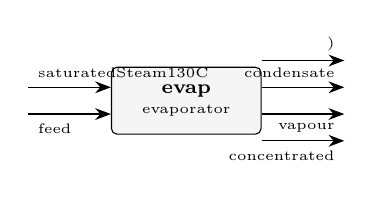
\begin{tikzpicture}[>={Stealth[length=2mm]}, every node/.style={font=\scriptsize}]
  \node[draw, rounded corners=2pt, align=center, minimum width=1.9cm, minimum height=0.85cm, fill=black!4] (evap) at (0.0,-0.0) {\textbf{evap}\\[-1pt]{\tiny evaporator}};
  \draw[->] ($(evap.west)+(-1.05,-0.17)$) -- ($(evap.west)+(0,-0.17)$) node[at start, below, font=\tiny, anchor=north west] {feed};
  \draw[->] ($(evap.west)+(-1.05,0.17)$) -- ($(evap.west)+(0,0.17)$) node[at start, above, font=\tiny, anchor=south west] {saturatedSteam130C};
  \draw[->] ($(evap.east)+(0,-0.51)$) -- ($(evap.east)+(1.05,-0.51)$) node[at end, below, font=\tiny, anchor=north east] {concentrated};
  \draw[->] ($(evap.east)+(0,-0.17)$) -- ($(evap.east)+(1.05,-0.17)$) node[at end, below, font=\tiny, anchor=north east] {vapour};
  \draw[->] ($(evap.east)+(0,0.17)$) -- ($(evap.east)+(1.05,0.17)$) node[at end, above, font=\tiny, anchor=south east] {condensate};
  \draw[->] ($(evap.east)+(0,0.51)$) -- ($(evap.east)+(1.05,0.51)$) node[at end, above, font=\tiny, anchor=south east] {)};
\end{tikzpicture}
\end{tutscheme}
\tutwhat{Single-effect NaOH evaporator: the heat of dilution IN the duty (fitted L\_phi, Parker-validated)}
\begin{tutnarrative}
- Choupo -$\ast$--------------------------------$\ast$ | \textbackslash\{\}|/ C hemicals | Choupo: open-source, glass-box simulation | | \textbackslash\{\}\textbackslash\{\}|// H eat-transfer | Version: Choupo-dev | | \textbackslash\{\}\textbackslash\{\}\textbackslash\{\}|/// O perations | Website: https://choupo.org | | \textbackslash\{\}\textbackslash\{\}|// U nits | Licence: GPL-3.0-or-later | | \textbackslash\{\}|/ P roperties | Tutorial case file -- part of Choupo | | | O ptimization | |

\end{tutnarrative}
\begin{tutgolden}
\goldrow{stream}{concentrated}{F}{0.0118365226457}
\goldrow{stream}{condensate}{F}{0.0208333333333}
\goldrow{stream}{feed}{F}{0.0277777777778}
\goldrow{stream}{saturatedSteam130C}{F}{0.0208333333333}
\goldrow{stream}{vapour}{F}{0.0159412551321}
\goldrow{kpi}{evap}{A}{20}
\goldrow{kpi}{evap}{A\_m2}{20}
\goldrow{kpi}{evap}{BPE}{6.45099255003}
\goldrow{kpi}{evap}{F\_conc}{0.0118365226457}
\goldrow{kpi}{evap}{F\_conc\_kmol\_h}{42.6114815246}
\goldrow{kpi}{evap}{F\_conc\_mass}{0.234606344352}
\goldrow{kpi}{evap}{F\_cond}{0.3753125}
\goldrow{kpi}{evap}{F\_cond\_kg\_h}{1351.125}
\goldrow{kpi}{evap}{F\_in}{0.0277777777778}
\goldmore{20}
\end{tutgolden}

\clearpage
\tutentry{evaporator09\_nacl\_sucrose\_brine}{tutorials/steady/evaporation/evaporator09\_nacl\_sucrose\_brine}
\begin{tutscheme}
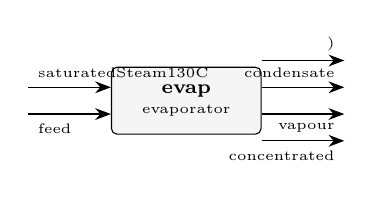
\begin{tikzpicture}[>={Stealth[length=2mm]}, every node/.style={font=\scriptsize}]
  \node[draw, rounded corners=2pt, align=center, minimum width=1.9cm, minimum height=0.85cm, fill=black!4] (evap) at (0.0,-0.0) {\textbf{evap}\\[-1pt]{\tiny evaporator}};
  \draw[->] ($(evap.west)+(-1.05,-0.17)$) -- ($(evap.west)+(0,-0.17)$) node[at start, below, font=\tiny, anchor=north west] {feed};
  \draw[->] ($(evap.west)+(-1.05,0.17)$) -- ($(evap.west)+(0,0.17)$) node[at start, above, font=\tiny, anchor=south west] {saturatedSteam130C};
  \draw[->] ($(evap.east)+(0,-0.51)$) -- ($(evap.east)+(1.05,-0.51)$) node[at end, below, font=\tiny, anchor=north east] {concentrated};
  \draw[->] ($(evap.east)+(0,-0.17)$) -- ($(evap.east)+(1.05,-0.17)$) node[at end, below, font=\tiny, anchor=north east] {vapour};
  \draw[->] ($(evap.east)+(0,0.17)$) -- ($(evap.east)+(1.05,0.17)$) node[at end, above, font=\tiny, anchor=south east] {condensate};
  \draw[->] ($(evap.east)+(0,0.51)$) -- ($(evap.east)+(1.05,0.51)$) node[at end, above, font=\tiny, anchor=south east] {)};
\end{tikzpicture}
\end{tutscheme}
\tutwhat{Evaporating a brine that also carries sugar: the electrolyte BPE is computed on the salt molality, and the rest is announced, not absorbed}
\begin{tutnarrative}
- Choupo -$\ast$--------------------------------$\ast$ | \textbackslash\{\}|/ C hemicals | Choupo: open-source, glass-box simulation | | \textbackslash\{\}\textbackslash\{\}|// H eat-transfer | Version: Choupo-dev | | \textbackslash\{\}\textbackslash\{\}\textbackslash\{\}|/// O perations | Website: https://choupo.org | | \textbackslash\{\}\textbackslash\{\}|// U nits | Licence: GPL-3.0-or-later | | \textbackslash\{\}|/ P roperties | Tutorial case file -- part of Choupo | | | O ptimization | |

\end{tutnarrative}
\begin{tutgolden}
\goldrow{stream}{concentrated}{F}{0.0211538965752}
\goldrow{stream}{condensate}{F}{0.0125}
\goldrow{stream}{feed}{F}{0.0281111111111}
\goldrow{stream}{saturatedSteam130C}{F}{0.0125}
\goldrow{stream}{vapour}{F}{0.00695721453587}
\goldrow{kpi}{evap}{A}{20}
\goldrow{kpi}{evap}{A\_m2}{20}
\goldrow{kpi}{evap}{BPE}{4.91270305537}
\goldrow{kpi}{evap}{F\_conc}{0.0211538965752}
\goldrow{kpi}{evap}{F\_conc\_kmol\_h}{76.1540276709}
\goldrow{kpi}{evap}{F\_conc\_mass}{0.545327280136}
\goldrow{kpi}{evap}{F\_cond}{0.2251875}
\goldrow{kpi}{evap}{F\_cond\_kg\_h}{810.675}
\goldrow{kpi}{evap}{F\_in}{0.0281111111111}
\goldmore{21}
\end{tutgolden}

\subsection{flash}
\grouptheory{flash}
\clearpage
\tutentry{adiabaticFlash01\_benzene\_toluene}{tutorials/steady/flash/adiabaticFlash01\_benzene\_toluene}
\begin{tutscheme}
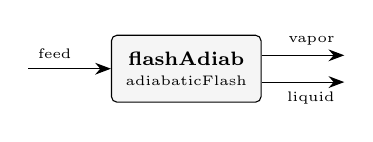
\begin{tikzpicture}[>={Stealth[length=2mm]}, every node/.style={font=\scriptsize}]
  \node[draw, rounded corners=2pt, align=center, minimum width=1.9cm, minimum height=0.85cm, fill=black!4] (flashAdiab) at (0.0,-0.0) {\textbf{flashAdiab}\\[-1pt]{\tiny adiabaticFlash}};
  \draw[->] ($(flashAdiab.west)+(-1.05,0.00)$) -- ($(flashAdiab.west)+(0,0.00)$) node[at start, above, font=\tiny, anchor=south west] {feed};
  \draw[->] ($(flashAdiab.east)+(0,-0.17)$) -- ($(flashAdiab.east)+(1.05,-0.17)$) node[at end, below, font=\tiny, anchor=north east] {liquid};
  \draw[->] ($(flashAdiab.east)+(0,0.17)$) -- ($(flashAdiab.east)+(1.05,0.17)$) node[at end, above, font=\tiny, anchor=south east] {vapor};
\end{tikzpicture}
\end{tutscheme}
\tutwhat{Adiabatic flash, benzene/toluene 40/60, 380K/3bar $\to$ 1atm}
\begin{tutnarrative}
- Choupo -$\ast$--------------------------------$\ast$ | \textbackslash\{\}|/ C hemicals | Choupo: open-source, glass-box simulation | | \textbackslash\{\}\textbackslash\{\}|// H eat-transfer | Version: Choupo-dev | | \textbackslash\{\}\textbackslash\{\}\textbackslash\{\}|/// O perations | Website: https://choupo.org | | \textbackslash\{\}\textbackslash\{\}|// U nits | Licence: GPL-3.0-or-later | | \textbackslash\{\}|/ P roperties | Tutorial case file -- part of Choupo | | | O ptimization | |

\end{tutnarrative}
\begin{tutgolden}
\goldrow{kpi}{flashAdiab}{T\_out}{368.661803634}
\goldrow{kpi}{flashAdiab}{V\_over\_F}{0.0518811133842}
\goldrow{stream}{feed}{F}{0.0277777777778}
\goldrow{stream}{liquid}{F}{0.0263366357393}
\goldrow{stream}{vapor}{F}{0.00144114203845}
\end{tutgolden}

\clearpage
\tutentry{analysis01\_water\_analysis\_inlet}{tutorials/steady/flash/analysis01\_water\_analysis\_inlet}
\begin{tutscheme}
\begin{tikzpicture}[>={Stealth[length=2mm]}, every node/.style={font=\scriptsize}]
  \node[draw, rounded corners=2pt, align=center, minimum width=1.9cm, minimum height=0.85cm, fill=black!4] (flash01) at (0.0,-0.0) {\textbf{flash01}\\[-1pt]{\tiny isothermalFlash}};
  \draw[->] ($(flash01.west)+(-1.05,0.00)$) -- ($(flash01.west)+(0,0.00)$) node[at start, above, font=\tiny, anchor=south west] {feed};
  \draw[->] ($(flash01.east)+(0,-0.17)$) -- ($(flash01.east)+(1.05,-0.17)$) node[at end, below, font=\tiny, anchor=north east] {liquid};
  \draw[->] ($(flash01.east)+(0,0.17)$) -- ($(flash01.east)+(1.05,0.17)$) node[at end, above, font=\tiny, anchor=south east] {vapor};
\end{tikzpicture}
\end{tutscheme}
\tutwhat{A laboratory water analysis as a first-class inlet: mg/L with alkalinity as CaCO3, a measured density, and a +0.78 \% ion imbalance reconciled onto chloride within a declared 10 \% limit -- measurement, reconciled inventory and equilibrium recorded as three separate layers}
\begin{tutnarrative}
- Choupo -$\ast$--------------------------------$\ast$ | analysis01 -- topology only (state lives in 0/) |

\end{tutnarrative}
\begin{tutgolden}
\goldrow{stream}{feed}{F}{0.0307824830015}
\goldrow{stream}{liquid}{F}{0.0307824830015}
\goldrow{stream}{vapor}{F}{0}
\goldrow{kpi}{flash01}{F\_alpha}{0.0307824830015}
\goldrow{kpi}{flash01}{F\_beta}{0}
\goldrow{kpi}{flash01}{F\_in}{0.0307824830015}
\goldrow{kpi}{flash01}{P}{101325}
\goldrow{kpi}{flash01}{T}{313.15}
\goldrow{kpi}{flash01}{V\_over\_F}{0}
\goldrow{kpi}{flash01}{pH}{7.90774504802}
\goldrow{kpi}{flash01}{p\_eq\_sum\_atm}{0.0747733964818}
\goldrow{kpi}{flash01}{phaseSet}{0}
\end{tutgolden}

\clearpage
\tutentry{analysis02\_weighted\_least\_squares}{tutorials/steady/flash/analysis02\_weighted\_least\_squares}
\begin{tutscheme}
\begin{tikzpicture}[>={Stealth[length=2mm]}, every node/.style={font=\scriptsize}]
  \node[draw, rounded corners=2pt, align=center, minimum width=1.9cm, minimum height=0.85cm, fill=black!4] (flash01) at (0.0,-0.0) {\textbf{flash01}\\[-1pt]{\tiny isothermalFlash}};
  \draw[->] ($(flash01.west)+(-1.05,0.00)$) -- ($(flash01.west)+(0,0.00)$) node[at start, above, font=\tiny, anchor=south west] {feed};
  \draw[->] ($(flash01.east)+(0,-0.17)$) -- ($(flash01.east)+(1.05,-0.17)$) node[at end, below, font=\tiny, anchor=north east] {liquid};
  \draw[->] ($(flash01.east)+(0,0.17)$) -- ($(flash01.east)+(1.05,0.17)$) node[at end, above, font=\tiny, anchor=south east] {vapor};
\end{tikzpicture}
\end{tutscheme}
\tutwhat{The same laboratory water as analysis01, reconciled by constrained weighted least squares over four measured quantities under electroneutrality plus an elemental-conservation redundancy: the correction spreads across all four at under 0.29 sigma each instead of shoving 5.12 \% into chloride}
\begin{tutnarrative}
- Choupo -$\ast$--------------------------------$\ast$ | analysis02 -- topology only (state lives in 0/) |

\end{tutnarrative}
\begin{tutgolden}
\goldrow{stream}{feed}{F}{0.0307825083878}
\goldrow{stream}{liquid}{F}{0.0307825083878}
\goldrow{stream}{vapor}{F}{0}
\goldrow{kpi}{flash01}{F\_alpha}{0.0307825083878}
\goldrow{kpi}{flash01}{F\_beta}{0}
\goldrow{kpi}{flash01}{F\_in}{0.0307825083878}
\goldrow{kpi}{flash01}{P}{101325}
\goldrow{kpi}{flash01}{T}{313.15}
\goldrow{kpi}{flash01}{V\_over\_F}{0}
\goldrow{kpi}{flash01}{pH}{7.90867882055}
\goldrow{kpi}{flash01}{p\_eq\_sum\_atm}{0.074797651023}
\goldrow{kpi}{flash01}{phaseSet}{0}
\end{tutgolden}

\clearpage
\tutentry{bubbleT01\_ethanol\_water}{tutorials/steady/flash/bubbleT01\_ethanol\_water}
\begin{tutscheme}
\begin{tikzpicture}[>={Stealth[length=2mm]}, every node/.style={font=\scriptsize}]
  \node[draw, rounded corners=2pt, align=center, minimum width=1.9cm, minimum height=0.85cm, fill=black!4] (bubble01) at (0.0,-0.0) {\textbf{bubble01}\\[-1pt]{\tiny bubbleT}};
  \draw[->] ($(bubble01.west)+(-1.05,0.00)$) -- ($(bubble01.west)+(0,0.00)$) node[at start, above, font=\tiny, anchor=south west] {feed};
\end{tikzpicture}
\end{tutscheme}
\tutwhat{Bubble-T of 30/70 ethanol/water at 1 atm (NRTL)}
\begin{tutnarrative}
- Choupo -$\ast$--------------------------------$\ast$ | \textbackslash\{\}|/ C hemicals | Choupo: open-source, glass-box simulation | | \textbackslash\{\}\textbackslash\{\}|// H eat-transfer | Version: Choupo-dev | | \textbackslash\{\}\textbackslash\{\}\textbackslash\{\}|/// O perations | Website: https://choupo.org | | \textbackslash\{\}\textbackslash\{\}|// U nits | Licence: GPL-3.0-or-later | | \textbackslash\{\}|/ P roperties | Tutorial case file -- part of Choupo | | | O ptimization | |

\end{tutnarrative}
\begin{tutgolden}
\goldrow{stream}{feed}{F}{0.0277777777778}
\goldrow{kpi}{bubble01}{P}{101325}
\goldrow{kpi}{bubble01}{T\_bubble}{354.424819099}
\goldrow{kpi}{bubble01}{converged}{1}
\goldrow{kpi}{bubble01}{y\_ethanol}{0.581915403358}
\goldrow{kpi}{bubble01}{y\_water}{0.418084596646}
\end{tutgolden}

\clearpage
\tutentry{bubbleT02\_uniquac\_ethanol\_water}{tutorials/steady/flash/bubbleT02\_uniquac\_ethanol\_water}
\begin{tutscheme}
\begin{tikzpicture}[>={Stealth[length=2mm]}, every node/.style={font=\scriptsize}]
  \node[draw, rounded corners=2pt, align=center, minimum width=1.9cm, minimum height=0.85cm, fill=black!4] (bubble02) at (0.0,-0.0) {\textbf{bubble02}\\[-1pt]{\tiny bubbleT}};
  \draw[->] ($(bubble02.west)+(-1.05,0.00)$) -- ($(bubble02.west)+(0,0.00)$) node[at start, above, font=\tiny, anchor=south west] {feed};
\end{tikzpicture}
\end{tutscheme}
\tutwhat{Bubble-T of 30/70 ethanol/water at 1 atm (UNIQUAC) -- validates the UNIQUAC model against the NRTL/Wilson twins}
\begin{tutnarrative}
- Choupo -$\ast$--------------------------------$\ast$ | \textbackslash\{\}|/ C hemicals | Choupo: open-source, glass-box simulation | | \textbackslash\{\}\textbackslash\{\}|// H eat-transfer | Version: Choupo-dev | | \textbackslash\{\}\textbackslash\{\}\textbackslash\{\}|/// O perations | Website: https://choupo.org | | \textbackslash\{\}\textbackslash\{\}|// U nits | Licence: GPL-3.0-or-later | | \textbackslash\{\}|/ P roperties | Tutorial case file -- part of Choupo | | | O ptimization | |

\end{tutnarrative}
\begin{tutgolden}
\goldrow{stream}{feed}{F}{0.0277777777778}
\goldrow{kpi}{bubble02}{P}{101325}
\goldrow{kpi}{bubble02}{T\_bubble}{353.469206954}
\goldrow{kpi}{bubble02}{converged}{1}
\goldrow{kpi}{bubble02}{y\_ethanol}{0.582711434226}
\goldrow{kpi}{bubble02}{y\_water}{0.417288565785}
\end{tutgolden}

\clearpage
\tutentry{dewT01\_ethanol\_water}{tutorials/steady/flash/dewT01\_ethanol\_water}
\begin{tutscheme}
\begin{tikzpicture}[>={Stealth[length=2mm]}, every node/.style={font=\scriptsize}]
  \node[draw, rounded corners=2pt, align=center, minimum width=1.9cm, minimum height=0.85cm, fill=black!4] (dew01) at (0.0,-0.0) {\textbf{dew01}\\[-1pt]{\tiny dewT}};
  \draw[->] ($(dew01.west)+(-1.05,0.00)$) -- ($(dew01.west)+(0,0.00)$) node[at start, above, font=\tiny, anchor=south west] {feed};
\end{tikzpicture}
\end{tutscheme}
\tutwhat{Dew-T of 30/70 ethanol/water vapour at 1 atm (NRTL)}
\begin{tutnarrative}
- Choupo -$\ast$--------------------------------$\ast$ | \textbackslash\{\}|/ C hemicals | Choupo: open-source, glass-box simulation | | \textbackslash\{\}\textbackslash\{\}|// H eat-transfer | Version: Choupo-dev | | \textbackslash\{\}\textbackslash\{\}\textbackslash\{\}|/// O perations | Website: https://choupo.org | | \textbackslash\{\}\textbackslash\{\}|// U nits | Licence: GPL-3.0-or-later | | \textbackslash\{\}|/ P roperties | Tutorial case file -- part of Choupo | | | O ptimization | |

\end{tutnarrative}
\begin{tutgolden}
\goldrow{stream}{feed}{F}{0.0277777777778}
\end{tutgolden}

\clearpage
\tutentry{flash01\_benzene\_toluene}{tutorials/steady/flash/flash01\_benzene\_toluene}
\begin{tutscheme}
\begin{tikzpicture}[>={Stealth[length=2mm]}, every node/.style={font=\scriptsize}]
  \node[draw, rounded corners=2pt, align=center, minimum width=1.9cm, minimum height=0.85cm, fill=black!4] (flash01) at (0.0,-0.0) {\textbf{flash01}\\[-1pt]{\tiny isothermalFlash}};
  \draw[->] ($(flash01.west)+(-1.05,0.00)$) -- ($(flash01.west)+(0,0.00)$) node[at start, above, font=\tiny, anchor=south west] {feed};
  \draw[->] ($(flash01.east)+(0,-0.17)$) -- ($(flash01.east)+(1.05,-0.17)$) node[at end, below, font=\tiny, anchor=north east] {liquid};
  \draw[->] ($(flash01.east)+(0,0.17)$) -- ($(flash01.east)+(1.05,0.17)$) node[at end, above, font=\tiny, anchor=south east] {vapor};
\end{tikzpicture}
\end{tutscheme}
\tutwhat{Isothermal flash benzene/toluene at 370 K, 1 bar (Raoult)}
\begin{tutnarrative}
- Choupo -$\ast$--------------------------------$\ast$ | \textbackslash\{\}|/ C hemicals | Choupo: open-source, glass-box simulation | | \textbackslash\{\}\textbackslash\{\}|// H eat-transfer | Version: Choupo-dev | | \textbackslash\{\}\textbackslash\{\}\textbackslash\{\}|/// O perations | Website: https://choupo.org | | \textbackslash\{\}\textbackslash\{\}|// U nits | Licence: GPL-3.0-or-later | | \textbackslash\{\}|/ P roperties | Tutorial case file -- part of Choupo | | | O ptimization | |

\end{tutnarrative}
\begin{tutgolden}
\goldrow{kpi}{flash01}{V\_over\_F}{0.30398357314}
\goldrow{kpi}{flash01}{T}{370}
\goldrow{stream}{vapor}{F}{0.00844398814279}
\goldrow{stream}{liquid}{F}{0.019333789635}
\end{tutgolden}

\clearpage
\tutentry{flash02\_ethanol\_water}{tutorials/steady/flash/flash02\_ethanol\_water}
\begin{tutscheme}
\begin{tikzpicture}[>={Stealth[length=2mm]}, every node/.style={font=\scriptsize}]
  \node[draw, rounded corners=2pt, align=center, minimum width=1.9cm, minimum height=0.85cm, fill=black!4] (flash02) at (0.0,-0.0) {\textbf{flash02}\\[-1pt]{\tiny isothermalFlash}};
  \draw[->] ($(flash02.west)+(-1.05,0.00)$) -- ($(flash02.west)+(0,0.00)$) node[at start, above, font=\tiny, anchor=south west] {feed};
  \draw[->] ($(flash02.east)+(0,-0.17)$) -- ($(flash02.east)+(1.05,-0.17)$) node[at end, below, font=\tiny, anchor=north east] {liquid};
  \draw[->] ($(flash02.east)+(0,0.17)$) -- ($(flash02.east)+(1.05,0.17)$) node[at end, above, font=\tiny, anchor=south east] {vapor};
\end{tikzpicture}
\end{tutscheme}
\tutwhat{Isothermal flash 50/50 ethanol/water at 355 K (NRTL)}
\begin{tutnarrative}
- Choupo -$\ast$--------------------------------$\ast$ | \textbackslash\{\}|/ C hemicals | Choupo: open-source, glass-box simulation | | \textbackslash\{\}\textbackslash\{\}|// H eat-transfer | Version: Choupo-dev | | \textbackslash\{\}\textbackslash\{\}\textbackslash\{\}|/// O perations | Website: https://choupo.org | | \textbackslash\{\}\textbackslash\{\}|// U nits | Licence: GPL-3.0-or-later | | \textbackslash\{\}|/ P roperties | Tutorial case file -- part of Choupo | | | O ptimization | |

\end{tutnarrative}
\begin{tutgolden}
\goldrow{stream}{feed}{F}{0.0277777777778}
\goldrow{stream}{liquid}{F}{0.00562323865754}
\goldrow{stream}{vapor}{F}{0.0221545391202}
\goldrow{kpi}{flash02}{F\_alpha}{0.00562323865754}
\goldrow{kpi}{flash02}{F\_beta}{0.0221545391202}
\goldrow{kpi}{flash02}{F\_in}{0.0277777777778}
\goldrow{kpi}{flash02}{P}{101325}
\goldrow{kpi}{flash02}{T}{355}
\goldrow{kpi}{flash02}{V\_over\_F}{0.797563408329}
\goldrow{kpi}{flash02}{phaseSet}{0}
\end{tutgolden}

\clearpage
\tutentry{flash03\_wilson\_ethanol\_water}{tutorials/steady/flash/flash03\_wilson\_ethanol\_water}
\begin{tutscheme}
\begin{tikzpicture}[>={Stealth[length=2mm]}, every node/.style={font=\scriptsize}]
  \node[draw, rounded corners=2pt, align=center, minimum width=1.9cm, minimum height=0.85cm, fill=black!4] (flash03) at (0.0,-0.0) {\textbf{flash03}\\[-1pt]{\tiny isothermalFlash}};
  \draw[->] ($(flash03.west)+(-1.05,0.00)$) -- ($(flash03.west)+(0,0.00)$) node[at start, above, font=\tiny, anchor=south west] {feed};
  \draw[->] ($(flash03.east)+(0,-0.17)$) -- ($(flash03.east)+(1.05,-0.17)$) node[at end, below, font=\tiny, anchor=north east] {liquid};
  \draw[->] ($(flash03.east)+(0,0.17)$) -- ($(flash03.east)+(1.05,0.17)$) node[at end, above, font=\tiny, anchor=south east] {vapor};
\end{tikzpicture}
\end{tutscheme}
\tutwhat{Isothermal flash 50/50 ethanol/water at 355 K (Wilson activity model)}
\begin{tutnarrative}
- Choupo -$\ast$--------------------------------$\ast$ | \textbackslash\{\}|/ C hemicals | Choupo: open-source, glass-box simulation | | \textbackslash\{\}\textbackslash\{\}|// H eat-transfer | Version: Choupo-dev | | \textbackslash\{\}\textbackslash\{\}\textbackslash\{\}|/// O perations | Website: https://choupo.org | | \textbackslash\{\}\textbackslash\{\}|// U nits | Licence: GPL-3.0-or-later | | \textbackslash\{\}|/ P roperties | Tutorial case file -- part of Choupo | | | O ptimization | |

\end{tutnarrative}
\begin{tutgolden}
\goldrow{stream}{feed}{F}{0.0277777777778}
\goldrow{stream}{liquid}{F}{0.0063767199082}
\goldrow{stream}{vapor}{F}{0.0214010578696}
\goldrow{kpi}{flash03}{F\_alpha}{0.0063767199082}
\goldrow{kpi}{flash03}{F\_beta}{0.0214010578696}
\goldrow{kpi}{flash03}{F\_in}{0.0277777777778}
\goldrow{kpi}{flash03}{P}{101325}
\goldrow{kpi}{flash03}{T}{355}
\goldrow{kpi}{flash03}{V\_over\_F}{0.770438083305}
\goldrow{kpi}{flash03}{phaseSet}{0}
\end{tutgolden}

\clearpage
\tutentry{flash04\_molarFlows\_input}{tutorials/steady/flash/flash04\_molarFlows\_input}
\begin{tutscheme}
\begin{tikzpicture}[>={Stealth[length=2mm]}, every node/.style={font=\scriptsize}]
  \node[draw, rounded corners=2pt, align=center, minimum width=1.9cm, minimum height=0.85cm, fill=black!4] (flash04) at (0.0,-0.0) {\textbf{flash04}\\[-1pt]{\tiny isothermalFlash}};
  \draw[->] ($(flash04.west)+(-1.05,0.00)$) -- ($(flash04.west)+(0,0.00)$) node[at start, above, font=\tiny, anchor=south west] {feed};
  \draw[->] ($(flash04.east)+(0,-0.17)$) -- ($(flash04.east)+(1.05,-0.17)$) node[at end, below, font=\tiny, anchor=north east] {liquid};
  \draw[->] ($(flash04.east)+(0,0.17)$) -- ($(flash04.east)+(1.05,0.17)$) node[at end, above, font=\tiny, anchor=south east] {vapor};
\end{tikzpicture}
\end{tutscheme}
\tutwhat{Isothermal flash, feed declared via molarFlows (benzene 40 + toluene 60 kmol/h)}
\begin{tutnarrative}
- Choupo -$\ast$--------------------------------$\ast$ | \textbackslash\{\}|/ C hemicals | Choupo: open-source, glass-box simulation | | \textbackslash\{\}\textbackslash\{\}|// H eat-transfer | Version: Choupo-dev | | \textbackslash\{\}\textbackslash\{\}\textbackslash\{\}|/// O perations | Website: https://choupo.org | | \textbackslash\{\}\textbackslash\{\}|// U nits | Licence: GPL-3.0-or-later | | \textbackslash\{\}|/ P roperties | Tutorial case file -- part of Choupo | | | O ptimization | |

\end{tutnarrative}
\begin{tutgolden}
\goldrow{stream}{feed}{F}{0.0277777777778}
\goldrow{stream}{liquid}{F}{0.019333789635}
\goldrow{stream}{vapor}{F}{0.00844398814279}
\goldrow{kpi}{flash04}{F\_alpha}{0.019333789635}
\goldrow{kpi}{flash04}{F\_beta}{0.00844398814279}
\goldrow{kpi}{flash04}{F\_in}{0.0277777777778}
\goldrow{kpi}{flash04}{P}{100000}
\goldrow{kpi}{flash04}{T}{370}
\goldrow{kpi}{flash04}{V\_over\_F}{0.30398357314}
\goldrow{kpi}{flash04}{phaseSet}{0}
\end{tutgolden}

\clearpage
\tutentry{flash05\_ternary\_massFlows}{tutorials/steady/flash/flash05\_ternary\_massFlows}
\begin{tutscheme}
\begin{tikzpicture}[>={Stealth[length=2mm]}, every node/.style={font=\scriptsize}]
  \node[draw, rounded corners=2pt, align=center, minimum width=1.9cm, minimum height=0.85cm, fill=black!4] (flash05) at (0.0,-0.0) {\textbf{flash05}\\[-1pt]{\tiny isothermalFlash}};
  \draw[->] ($(flash05.west)+(-1.05,0.00)$) -- ($(flash05.west)+(0,0.00)$) node[at start, above, font=\tiny, anchor=south west] {feed};
  \draw[->] ($(flash05.east)+(0,-0.17)$) -- ($(flash05.east)+(1.05,-0.17)$) node[at end, below, font=\tiny, anchor=north east] {liquid};
  \draw[->] ($(flash05.east)+(0,0.17)$) -- ($(flash05.east)+(1.05,0.17)$) node[at end, above, font=\tiny, anchor=south east] {vapor};
\end{tikzpicture}
\end{tutscheme}
\tutwhat{Ternary flash benzene/toluene/n-hexane, feed in mass flows (5000 kg/h)}
\begin{tutnarrative}
- Choupo -$\ast$--------------------------------$\ast$ | \textbackslash\{\}|/ C hemicals | Choupo: open-source, glass-box simulation | | \textbackslash\{\}\textbackslash\{\}|// H eat-transfer | Version: Choupo-dev | | \textbackslash\{\}\textbackslash\{\}\textbackslash\{\}|/// O perations | Website: https://choupo.org | | \textbackslash\{\}\textbackslash\{\}|// U nits | Licence: GPL-3.0-or-later | | \textbackslash\{\}|/ P roperties | Tutorial case file -- part of Choupo | | | O ptimization | |

\end{tutnarrative}
\begin{tutgolden}
\goldrow{stream}{feed}{F}{0.0160941453232}
\goldrow{stream}{liquid}{F}{0.00814913402453}
\goldrow{stream}{vapor}{F}{0.00794501129864}
\goldrow{kpi}{flash05}{F\_alpha}{0.00814913402453}
\goldrow{kpi}{flash05}{F\_beta}{0.00794501129864}
\goldrow{kpi}{flash05}{F\_in}{0.0160941453232}
\goldrow{kpi}{flash05}{P}{100000}
\goldrow{kpi}{flash05}{T}{365}
\goldrow{kpi}{flash05}{V\_over\_F}{0.493658478851}
\goldrow{kpi}{flash05}{phaseSet}{0}
\end{tutgolden}

\clearpage
\tutentry{flash06\_sweep\_T}{tutorials/steady/flash/flash06\_sweep\_T}
\begin{tutscheme}
\begin{tikzpicture}[>={Stealth[length=2mm]}, every node/.style={font=\scriptsize}]
  \node[draw, rounded corners=2pt, align=center, minimum width=1.9cm, minimum height=0.85cm, fill=black!4] (flash01) at (0.0,-0.0) {\textbf{flash01}\\[-1pt]{\tiny isothermalFlash}};
  \draw[->] ($(flash01.west)+(-1.05,0.00)$) -- ($(flash01.west)+(0,0.00)$) node[at start, above, font=\tiny, anchor=south west] {feed};
  \draw[->] ($(flash01.east)+(0,-0.17)$) -- ($(flash01.east)+(1.05,-0.17)$) node[at end, below, font=\tiny, anchor=north east] {liquid};
  \draw[->] ($(flash01.east)+(0,0.17)$) -- ($(flash01.east)+(1.05,0.17)$) node[at end, above, font=\tiny, anchor=south east] {vapor};
\end{tikzpicture}
\end{tutscheme}
\tutwhat{Flash benzene/toluene at 1 bar: T swept 360$\to$385 K across the bubble$\to$dew window (V/F S-curve + duty)}
\begin{tutnarrative}
- Choupo -$\ast$--------------------------------$\ast$ | \textbackslash\{\}|/ C hemicals | Choupo: open-source, glass-box simulation | | \textbackslash\{\}\textbackslash\{\}|// H eat-transfer | Version: Choupo-dev | | \textbackslash\{\}\textbackslash\{\}\textbackslash\{\}|/// O perations | Website: https://choupo.org | | \textbackslash\{\}\textbackslash\{\}|// U nits | Licence: GPL-3.0-or-later | | \textbackslash\{\}|/ P roperties | Tutorial case file -- part of Choupo | | | O ptimization | |

\end{tutnarrative}

\clearpage
\tutentry{flash07\_gridsweep\_TP}{tutorials/steady/flash/flash07\_gridsweep\_TP}
\begin{tutscheme}
\begin{tikzpicture}[>={Stealth[length=2mm]}, every node/.style={font=\scriptsize}]
  \node[draw, rounded corners=2pt, align=center, minimum width=1.9cm, minimum height=0.85cm, fill=black!4] (flashDrum) at (0.0,-0.0) {\textbf{flashDrum}\\[-1pt]{\tiny isothermalFlash}};
  \draw[->] ($(flashDrum.west)+(-1.05,0.00)$) -- ($(flashDrum.west)+(0,0.00)$) node[at start, above, font=\tiny, anchor=south west] {feed};
  \draw[->] ($(flashDrum.east)+(0,-0.17)$) -- ($(flashDrum.east)+(1.05,-0.17)$) node[at end, below, font=\tiny, anchor=north east] {liquid};
  \draw[->] ($(flashDrum.east)+(0,0.17)$) -- ($(flashDrum.east)+(1.05,0.17)$) node[at end, above, font=\tiny, anchor=south east] {vapor};
\end{tikzpicture}
\end{tutscheme}
\tutwhat{2-D grid sweep: flash V/F over T x P (the flash envelope)}
\begin{tutnarrative}
- Choupo -$\ast$--------------------------------$\ast$ | \textbackslash\{\}|/ C hemicals | Choupo: open-source, glass-box simulation | | \textbackslash\{\}\textbackslash\{\}|// H eat-transfer | Version: Choupo-dev | | \textbackslash\{\}\textbackslash\{\}\textbackslash\{\}|/// O perations | Website: https://choupo.org | | \textbackslash\{\}\textbackslash\{\}|// U nits | Licence: GPL-3.0-or-later | | \textbackslash\{\}|/ P roperties | Tutorial case file -- part of Choupo | | | O ptimization | |

\end{tutnarrative}

\clearpage
\tutentry{flash08\_co2\_water\_package}{tutorials/steady/flash/flash08\_co2\_water\_package}
\tutwhat{Carbonated water flash whose thermo is an INLINE property-package MANIFEST: constant/thermoPhysPropDict IS the full record (components, methods per phase, solvent+solutes, the CO2-water Henry pair declared+verified). CO2 dissolves by the unsymmetric Henry convention; water stays Raoult. Read the run log: the assembly announces itself.}
\begin{tutnarrative}
- Choupo -$\ast$--------------------------------$\ast$ | \textbackslash\{\}|/ C hemicals | Choupo: open-source, glass-box simulation | | \textbackslash\{\}\textbackslash\{\}|// H eat-transfer | Version: Choupo-dev | | \textbackslash\{\}\textbackslash\{\}\textbackslash\{\}|/// O perations | Website: https://choupo.org | | \textbackslash\{\}\textbackslash\{\}|// U nits | Licence: GPL-3.0-or-later | | \textbackslash\{\}|/ P roperties | Tutorial case file -- part of Choupo | | | O ptimization | |

\end{tutnarrative}
\begin{tutgolden}
\goldrow{stream}{flatWater}{F}{0.000277662593734}
\goldrow{stream}{gasOff}{F}{1.15184043824e-07}
\goldrow{stream}{sodaWater}{F}{0.000277777777778}
\goldrow{kpi}{node}{F\_alpha}{0.000277662593734}
\goldrow{kpi}{node}{F\_beta}{1.15184043824e-07}
\goldrow{kpi}{node}{F\_in}{0.000277777777778}
\goldrow{kpi}{node}{P}{101325}
\goldrow{kpi}{node}{Q}{0}
\goldrow{kpi}{node}{Q\_kW}{0}
\goldrow{kpi}{node}{T}{298.15}
\goldrow{kpi}{node}{V\_over\_F}{0.000414662557767}
\goldrow{kpi}{node}{phaseSet}{0}
\end{tutgolden}

\clearpage
\tutentry{flash09\_n2ch4\_stryjek}{tutorials/steady/flash/flash09\_n2ch4\_stryjek}
\tutwhat{phi-phi VLE VALIDATION vs Stryjek, Chappelear \& Kobayashi (1974), J. Chem. Eng. Data 19:334 (DOI 10.1021/je60063a023), Table III, -190 F = 149.82 K. The case carries its thermo as an INLINE manifest: liquid+vapour both eos.SRK (one cubic, two roots: K = phi\_L/phi\_V) with the N2-CH4 interaction constant kij = 0.0289 (a small measured correction to the mixing rule, from the Knapp/DECHEMA data compilation). Measured at 299 psia: x\_N2=0.1503, y\_N2=0.4579 -- compare the Flash Result table in the log with these measured values (agreement \textasciitilde{}2\%).}
\begin{tutnarrative}
- Choupo -$\ast$--------------------------------$\ast$ | \textbackslash\{\}|/ C hemicals | Choupo: open-source, glass-box simulation | | \textbackslash\{\}\textbackslash\{\}|// H eat-transfer | Version: Choupo-dev | | \textbackslash\{\}\textbackslash\{\}\textbackslash\{\}|/// O perations | Website: https://choupo.org | | \textbackslash\{\}\textbackslash\{\}|// U nits | Licence: GPL-3.0-or-later | | \textbackslash\{\}|/ P roperties | Tutorial case file -- part of Choupo | | | O ptimization | |

\end{tutnarrative}
\begin{tutgolden}
\goldrow{stream}{feed}{F}{0.000277777777778}
\goldrow{stream}{liq}{F}{0.000145628387466}
\goldrow{stream}{vap}{F}{0.000132149390312}
\goldrow{kpi}{node}{F\_alpha}{0.000145628387466}
\goldrow{kpi}{node}{F\_beta}{0.000132149390312}
\goldrow{kpi}{node}{F\_in}{0.000277777777778}
\goldrow{kpi}{node}{P}{2061600}
\goldrow{kpi}{node}{Q}{0}
\goldrow{kpi}{node}{Q\_kW}{0}
\goldrow{kpi}{node}{T}{149.82}
\goldrow{kpi}{node}{V\_over\_F}{0.475737805121}
\goldrow{kpi}{node}{phaseSet}{0}
\goldrow{kpi}{node}{K\_N2}{3.047}
\goldrow{kpi}{node}{K\_CH4}{0.638}
\end{tutgolden}

\clearpage
\tutentry{flash09\_nh3\_water\_reactive}{tutorials/steady/flash/flash09\_nh3\_water\_reactive}
\begin{tutscheme}
\begin{tikzpicture}[>={Stealth[length=2mm]}, every node/.style={font=\scriptsize}]
  \node[draw, rounded corners=2pt, align=center, minimum width=1.9cm, minimum height=0.85cm, fill=black!4] (flash01) at (0.0,-0.0) {\textbf{flash01}\\[-1pt]{\tiny isothermalFlash}};
  \draw[->] ($(flash01.west)+(-1.05,0.00)$) -- ($(flash01.west)+(0,0.00)$) node[at start, above, font=\tiny, anchor=south west] {feed};
  \draw[->] ($(flash01.east)+(0,-0.17)$) -- ($(flash01.east)+(1.05,-0.17)$) node[at end, below, font=\tiny, anchor=north east] {liquid};
  \draw[->] ($(flash01.east)+(0,0.17)$) -- ($(flash01.east)+(1.05,0.17)$) node[at end, above, font=\tiny, anchor=south east] {vapor};
\end{tikzpicture}
\end{tutscheme}
\tutwhat{Reactive NH3/water flash: SIMULTANEOUS aqueous speciation (NH4+/H+/OH-, pH solved) + VLE at 368 K, 1 atm -- ions never reach the vapour or the streams}
\begin{tutnarrative}
- Choupo -$\ast$--------------------------------$\ast$ | \textbackslash\{\}|/ C hemicals | Choupo: open-source, glass-box simulation | | \textbackslash\{\}\textbackslash\{\}|// H eat-transfer | Version: Choupo-dev | | \textbackslash\{\}\textbackslash\{\}\textbackslash\{\}|/// O perations | Website: https://choupo.org | | \textbackslash\{\}\textbackslash\{\}|// U nits | Licence: GPL-3.0-or-later | | \textbackslash\{\}|/ P roperties | Tutorial case file -- part of Choupo | | | O ptimization | |

\end{tutnarrative}
\begin{tutgolden}
\goldrow{stream}{feed}{F}{0.0277777777778}
\goldrow{stream}{liquid}{F}{0.0224533469429}
\goldrow{stream}{vapor}{F}{0.00532443083488}
\goldrow{kpi}{flash01}{F\_alpha}{0.0224533469429}
\goldrow{kpi}{flash01}{F\_beta}{0.00532443083488}
\goldrow{kpi}{flash01}{F\_in}{0.0277777777778}
\goldrow{kpi}{flash01}{P}{101325}
\goldrow{kpi}{flash01}{Q}{0}
\goldrow{kpi}{flash01}{Q\_kW}{0}
\goldrow{kpi}{flash01}{T}{368.15}
\goldrow{kpi}{flash01}{V\_over\_F}{0.191679510056}
\goldrow{kpi}{flash01}{pH}{9.899823444}
\goldrow{kpi}{flash01}{p\_eq\_sum\_atm}{1}
\goldrow{kpi}{flash01}{phaseSet}{0}
\end{tutgolden}

\clearpage
\tutentry{flash10\_acetic\_water\_reactive}{tutorials/steady/flash/flash10\_acetic\_water\_reactive}
\begin{tutscheme}
\begin{tikzpicture}[>={Stealth[length=2mm]}, every node/.style={font=\scriptsize}]
  \node[draw, rounded corners=2pt, align=center, minimum width=1.9cm, minimum height=0.85cm, fill=black!4] (flash01) at (0.0,-0.0) {\textbf{flash01}\\[-1pt]{\tiny isothermalFlash}};
  \draw[->] ($(flash01.west)+(-1.05,0.00)$) -- ($(flash01.west)+(0,0.00)$) node[at start, above, font=\tiny, anchor=south west] {feed};
  \draw[->] ($(flash01.east)+(0,-0.17)$) -- ($(flash01.east)+(1.05,-0.17)$) node[at end, below, font=\tiny, anchor=north east] {liquid};
  \draw[->] ($(flash01.east)+(0,0.17)$) -- ($(flash01.east)+(1.05,0.17)$) node[at end, above, font=\tiny, anchor=south east] {vapor};
\end{tikzpicture}
\end{tutscheme}
\tutwhat{Reactive acetic acid/water flash: SIMULTANEOUS aqueous speciation (Acetate-/H+/OH-, pH solved) + VLE -- the weak ACID mirror of flash09; ions never reach the vapour or the streams}
\begin{tutnarrative}
- Choupo -$\ast$--------------------------------$\ast$ | \textbackslash\{\}|/ C hemicals | Choupo: open-source, glass-box simulation | | \textbackslash\{\}\textbackslash\{\}|// H eat-transfer | Version: Choupo-dev | | \textbackslash\{\}\textbackslash\{\}\textbackslash\{\}|/// O perations | Website: https://choupo.org | | \textbackslash\{\}\textbackslash\{\}|// U nits | Licence: GPL-3.0-or-later | | \textbackslash\{\}|/ P roperties | Tutorial case file -- part of Choupo | | | O ptimization | |

\end{tutnarrative}
\begin{tutgolden}
\goldrow{stream}{feed}{F}{0.0277777777778}
\goldrow{stream}{liquid}{F}{0.0277777777778}
\goldrow{stream}{vapor}{F}{0}
\goldrow{kpi}{flash01}{F\_alpha}{0.0277777777778}
\goldrow{kpi}{flash01}{F\_beta}{0}
\goldrow{kpi}{flash01}{F\_in}{0.0277777777778}
\goldrow{kpi}{flash01}{P}{101325}
\goldrow{kpi}{flash01}{Q}{0}
\goldrow{kpi}{flash01}{Q\_kW}{0}
\goldrow{kpi}{flash01}{T}{368.15}
\goldrow{kpi}{flash01}{V\_over\_F}{0}
\goldrow{kpi}{flash01}{dimer\_share}{0.369144977061}
\goldrow{kpi}{flash01}{pH}{2.15260602547}
\goldrow{kpi}{flash01}{p\_dimer\_atm}{0.0217386638116}
\goldmore{3}
\end{tutgolden}

\clearpage
\tutentry{flash10\_ch4propane\_pcsaft}{tutorials/steady/flash/flash10\_ch4propane\_pcsaft}
\tutwhat{PC-SAFT phi-phi binary flash, CH4/propane at 273.15 K / 20 bar, kij = 0 (announced): the PREDICTIVE baseline of the SAFT world -- K = phi\_L/phi\_V from ONE a\_res surface at its two density roots. Sanity anchor carried by the case itself: propane's curated Antoine gives Psat(273.15 K) = 4.7 bar, so the Raoult-magnitude K\_propane \textasciitilde{} 0.24 -- the PC-SAFT K\_propane = 0.32 sits near it (the deviation IS the fugacity correction of a liquid holding \textasciitilde{}11\% dissolved CH4, visible); K\_CH4 >> 1 (supercritical light key). The published-kij refinement is a NAMED follow-up: it needs the cited pair record (data/standards/parameters/PCSAFT/), never an invented number.}
\begin{tutnarrative}
- Choupo -$\ast$--------------------------------$\ast$ | \textbackslash\{\}|/ C hemicals | Choupo: open-source, glass-box simulation | | \textbackslash\{\}\textbackslash\{\}|// H eat-transfer | Version: Choupo-dev | | \textbackslash\{\}\textbackslash\{\}\textbackslash\{\}|/// O perations | Website: https://choupo.org | | \textbackslash\{\}\textbackslash\{\}|// U nits | Licence: GPL-3.0-or-later | | \textbackslash\{\}|/ P roperties | Tutorial case file -- part of Choupo | | | O ptimization | |

\end{tutnarrative}
\begin{tutgolden}
\goldrow{stream}{feed}{F}{0.000277777777778}
\goldrow{stream}{liq}{F}{9.97838549688e-05}
\goldrow{stream}{vap}{F}{0.000177993922809}
\goldrow{kpi}{node}{F\_alpha}{9.97838549688e-05}
\goldrow{kpi}{node}{F\_beta}{0.000177993922809}
\goldrow{kpi}{node}{F\_in}{0.000277777777778}
\goldrow{kpi}{node}{P}{2000000}
\goldrow{kpi}{node}{Q}{0}
\goldrow{kpi}{node}{Q\_kW}{0}
\goldrow{kpi}{node}{T}{273.15}
\goldrow{kpi}{node}{V\_over\_F}{0.640778122112}
\goldrow{kpi}{node}{phaseSet}{0}
\end{tutgolden}

\clearpage
\tutentry{flash11\_acetic\_T\_sweep}{tutorials/steady/flash/flash11\_acetic\_T\_sweep}
\begin{tutscheme}
\begin{tikzpicture}[>={Stealth[length=2mm]}, every node/.style={font=\scriptsize}]
  \node[draw, rounded corners=2pt, align=center, minimum width=1.9cm, minimum height=0.85cm, fill=black!4] (flash01) at (0.0,-0.0) {\textbf{flash01}\\[-1pt]{\tiny isothermalFlash}};
  \draw[->] ($(flash01.west)+(-1.05,0.00)$) -- ($(flash01.west)+(0,0.00)$) node[at start, above, font=\tiny, anchor=south west] {feed};
  \draw[->] ($(flash01.east)+(0,-0.17)$) -- ($(flash01.east)+(1.05,-0.17)$) node[at end, below, font=\tiny, anchor=north east] {liquid};
  \draw[->] ($(flash01.east)+(0,0.17)$) -- ($(flash01.east)+(1.05,0.17)$) node[at end, above, font=\tiny, anchor=south east] {vapor};
\end{tikzpicture}
\end{tutscheme}
\tutwhat{Reactive acetic/water flash: T swept 328$\to$368 K in the subsaturated window (p\_eq climbs, dimer share falls, pH drifts)}
\begin{tutnarrative}
- Choupo -$\ast$--------------------------------$\ast$ | \textbackslash\{\}|/ C hemicals | Choupo: open-source, glass-box simulation | | \textbackslash\{\}\textbackslash\{\}|// H eat-transfer | Version: Choupo-dev | | \textbackslash\{\}\textbackslash\{\}\textbackslash\{\}|/// O perations | Website: https://choupo.org | | \textbackslash\{\}\textbackslash\{\}|// U nits | Licence: GPL-3.0-or-later | | \textbackslash\{\}|/ P roperties | Tutorial case file -- part of Choupo | | | O ptimization | |

\end{tutnarrative}

\clearpage
\tutentry{flash12\_nh3\_acetic\_ethanol\_reactive}{tutorials/steady/flash/flash12\_nh3\_acetic\_ethanol\_reactive}
\begin{tutscheme}
\begin{tikzpicture}[>={Stealth[length=2mm]}, every node/.style={font=\scriptsize}]
  \node[draw, rounded corners=2pt, align=center, minimum width=1.9cm, minimum height=0.85cm, fill=black!4] (flash01) at (0.0,-0.0) {\textbf{flash01}\\[-1pt]{\tiny isothermalFlash}};
  \draw[->] ($(flash01.west)+(-1.05,0.00)$) -- ($(flash01.west)+(0,0.00)$) node[at start, above, font=\tiny, anchor=south west] {feed};
  \draw[->] ($(flash01.east)+(0,-0.17)$) -- ($(flash01.east)+(1.05,-0.17)$) node[at end, below, font=\tiny, anchor=north east] {liquid};
  \draw[->] ($(flash01.east)+(0,0.17)$) -- ($(flash01.east)+(1.05,0.17)$) node[at end, above, font=\tiny, anchor=south east] {vapor};
\end{tikzpicture}
\end{tutscheme}
\tutwhat{Reactive 4-component flash: NH3 + HAc neutralise into an ammonium-acetate buffer (pH \textasciitilde{} pKa\_HAc); ethanol classified nonionising from its record fact, ideal VLE authorised; subsaturated at 358.15 K}
\begin{tutnarrative}
- Choupo -$\ast$--------------------------------$\ast$ | \textbackslash\{\}|/ C hemicals | Choupo: open-source, glass-box simulation | | \textbackslash\{\}\textbackslash\{\}|// H eat-transfer | Version: Choupo-dev | | \textbackslash\{\}\textbackslash\{\}\textbackslash\{\}|/// O perations | Website: https://choupo.org | | \textbackslash\{\}\textbackslash\{\}|// U nits | Licence: GPL-3.0-or-later | | \textbackslash\{\}|/ P roperties | Tutorial case file -- part of Choupo | | | O ptimization | |

\end{tutnarrative}
\begin{tutgolden}
\goldrow{stream}{feed}{F}{0.0277777777778}
\goldrow{stream}{liquid}{F}{0.0277777777778}
\goldrow{stream}{vapor}{F}{0}
\goldrow{kpi}{flash01}{F\_alpha}{0.0277777777778}
\goldrow{kpi}{flash01}{F\_beta}{0}
\goldrow{kpi}{flash01}{F\_in}{0.0277777777778}
\goldrow{kpi}{flash01}{P}{101325}
\goldrow{kpi}{flash01}{Q}{0}
\goldrow{kpi}{flash01}{Q\_kW}{0}
\goldrow{kpi}{flash01}{T}{358.15}
\goldrow{kpi}{flash01}{V\_over\_F}{0}
\goldrow{kpi}{flash01}{dimer\_share}{0.110194123555}
\goldrow{kpi}{flash01}{pH}{4.6182465052}
\goldrow{kpi}{flash01}{p\_dimer\_atm}{0.000571052689738}
\goldmore{4}
\end{tutgolden}

\clearpage
\tutentry{flash13\_acetic\_ethanol\_vacuum\_flash}{tutorials/steady/flash/flash13\_acetic\_ethanol\_vacuum\_flash}
\begin{tutscheme}
\begin{tikzpicture}[>={Stealth[length=2mm]}, every node/.style={font=\scriptsize}]
  \node[draw, rounded corners=2pt, align=center, minimum width=1.9cm, minimum height=0.85cm, fill=black!4] (flash01) at (0.0,-0.0) {\textbf{flash01}\\[-1pt]{\tiny isothermalFlash}};
  \draw[->] ($(flash01.west)+(-1.05,0.00)$) -- ($(flash01.west)+(0,0.00)$) node[at start, above, font=\tiny, anchor=south west] {feed};
  \draw[->] ($(flash01.east)+(0,-0.17)$) -- ($(flash01.east)+(1.05,-0.17)$) node[at end, below, font=\tiny, anchor=north east] {liquid};
  \draw[->] ($(flash01.east)+(0,0.17)$) -- ($(flash01.east)+(1.05,0.17)$) node[at end, above, font=\tiny, anchor=south east] {vapor};
\end{tikzpicture}
\end{tutscheme}
\tutwhat{Reactive VACUUM flash on mixed-solvent v1 (NRTL backbone + Davies ions): V/F = 0.58 at 358.15 K / 0.65 atm, gamma\_EtOH = 2.97, the buffer holds the ammonia, dimer heat priced exactly}
\begin{tutnarrative}
- Choupo -$\ast$--------------------------------$\ast$ | \textbackslash\{\}|/ C hemicals | Choupo: open-source, glass-box simulation | | \textbackslash\{\}\textbackslash\{\}|// H eat-transfer | Version: Choupo-dev | | \textbackslash\{\}\textbackslash\{\}\textbackslash\{\}|/// O perations | Website: https://choupo.org | | \textbackslash\{\}\textbackslash\{\}|// U nits | Licence: GPL-3.0-or-later | | \textbackslash\{\}|/ P roperties | Tutorial case file -- part of Choupo | | | O ptimization | |

\end{tutnarrative}
\begin{tutgolden}
\goldrow{stream}{feed}{F}{0.0277777777778}
\goldrow{stream}{liquid}{F}{0.011654196993}
\goldrow{stream}{vapor}{F}{0.0161235807848}
\goldrow{kpi}{flash01}{F\_alpha}{0.011654196993}
\goldrow{kpi}{flash01}{F\_beta}{0.0161235807848}
\goldrow{kpi}{flash01}{F\_in}{0.0277777777778}
\goldrow{kpi}{flash01}{P}{65861.25}
\goldrow{kpi}{flash01}{Q}{669288.026161}
\goldrow{kpi}{flash01}{Q\_kW}{669.288026161}
\goldrow{kpi}{flash01}{T}{358.15}
\goldrow{kpi}{flash01}{V\_over\_F}{0.580448908254}
\goldrow{kpi}{flash01}{dimer\_share}{0.121262947986}
\goldrow{kpi}{flash01}{pH}{5.02590694419}
\goldrow{kpi}{flash01}{p\_dimer\_atm}{0.000709068539902}
\goldmore{8}
\end{tutgolden}

\clearpage
\tutentry{flash14\_calcite\_carbonate\_basis}{tutorials/steady/flash/flash14\_calcite\_carbonate\_basis}
\begin{tutscheme}
\begin{tikzpicture}[>={Stealth[length=2mm]}, every node/.style={font=\scriptsize}]
  \node[draw, rounded corners=2pt, align=center, minimum width=1.9cm, minimum height=0.85cm, fill=black!4] (flash01) at (0.0,-0.0) {\textbf{flash01}\\[-1pt]{\tiny isothermalFlash}};
  \draw[->] ($(flash01.west)+(-1.05,0.00)$) -- ($(flash01.west)+(0,0.00)$) node[at start, above, font=\tiny, anchor=south west] {feed};
  \draw[->] ($(flash01.east)+(0,-0.17)$) -- ($(flash01.east)+(1.05,-0.17)$) node[at end, below, font=\tiny, anchor=north east] {liquid};
  \draw[->] ($(flash01.east)+(0,0.17)$) -- ($(flash01.east)+(1.05,0.17)$) node[at end, above, font=\tiny, anchor=south east] {vapor};
\end{tikzpicture}
\end{tutscheme}
\tutwhat{Reactive calcite/carbonate flash: the FIRST component whose aqueous bridge spans TWO master families (CaCO3 $\to$ Ca+2 AND HCO3-), so the component-to-species map is a matrix, not a renaming}
\begin{tutnarrative}
- Choupo -$\ast$--------------------------------$\ast$ | flash14 -- topology only (state lives in 0/) |

\end{tutnarrative}
\begin{tutgolden}
\goldrow{stream}{feed}{F}{0.0275033888889}
\goldrow{stream}{liquid}{F}{0.0269197611327}
\goldrow{stream}{vapor}{F}{0.000583627756178}
\goldrow{kpi}{flash01}{F\_alpha}{0.0269197611327}
\goldrow{kpi}{flash01}{F\_beta}{0.000583627756178}
\goldrow{kpi}{flash01}{F\_in}{0.0275033888889}
\goldrow{kpi}{flash01}{P}{101325}
\goldrow{kpi}{flash01}{T}{313.15}
\goldrow{kpi}{flash01}{V\_over\_F}{0.0212202124813}
\goldrow{kpi}{flash01}{pH}{6.01561221041}
\goldrow{kpi}{flash01}{p\_eq\_sum\_atm}{1}
\goldrow{kpi}{flash01}{phaseSet}{0}
\end{tutgolden}

\clearpage
\tutentry{flash15\_refused\_salt\_basis\_rank}{tutorials/steady/flash/flash15\_refused\_salt\_basis\_rank}
\begin{tutscheme}
\begin{tikzpicture}[>={Stealth[length=2mm]}, every node/.style={font=\scriptsize}]
  \node[draw, rounded corners=2pt, align=center, minimum width=1.9cm, minimum height=0.85cm, fill=black!4] (flash01) at (0.0,-0.0) {\textbf{flash01}\\[-1pt]{\tiny isothermalFlash}};
  \draw[->] ($(flash01.west)+(-1.05,0.00)$) -- ($(flash01.west)+(0,0.00)$) node[at start, above, font=\tiny, anchor=south west] {feed};
  \draw[->] ($(flash01.east)+(0,-0.17)$) -- ($(flash01.east)+(1.05,-0.17)$) node[at end, below, font=\tiny, anchor=north east] {liquid};
  \draw[->] ($(flash01.east)+(0,0.17)$) -- ($(flash01.east)+(1.05,0.17)$) node[at end, above, font=\tiny, anchor=south east] {vapor};
\end{tikzpicture}
\end{tutscheme}
\tutwhat{DELIBERATE REFUSAL: K/Na x Cl/SO4 -- four salt components onto four ion families with rank 3, so the component basis has exactly (c-1)(a-1) = 1 degree of freedom and the converged state cannot be read back as these components uniquely}
\begin{tutnarrative}
- Choupo -$\ast$--------------------------------$\ast$ | \textbackslash\{\}|/ C hemicals | Choupo: open-source, glass-box simulation | | \textbackslash\{\}\textbackslash\{\}|// H eat-transfer | Version: Choupo-dev | | \textbackslash\{\}\textbackslash\{\}\textbackslash\{\}|/// O perations | Website: https://choupo.org | | \textbackslash\{\}|/ P roperties | Tutorial case file -- part of Choupo | | | O ptimization | DELIBERATE REFUSAL -- this case must NOT run |

\end{tutnarrative}

\clearpage
\tutentry{flash16\_calcite\_precipitation}{tutorials/steady/flash/flash16\_calcite\_precipitation}
\begin{tutscheme}
\begin{tikzpicture}[>={Stealth[length=2mm]}, every node/.style={font=\scriptsize}]
  \node[draw, rounded corners=2pt, align=center, minimum width=1.9cm, minimum height=0.85cm, fill=black!4] (flash01) at (0.0,-0.0) {\textbf{flash01}\\[-1pt]{\tiny isothermalFlash}};
  \draw[->] ($(flash01.west)+(-1.05,0.00)$) -- ($(flash01.west)+(0,0.00)$) node[at start, above, font=\tiny, anchor=south west] {feed};
  \draw[->] ($(flash01.east)+(0,-0.17)$) -- ($(flash01.east)+(1.05,-0.17)$) node[at end, below, font=\tiny, anchor=north east] {liquid};
  \draw[->] ($(flash01.east)+(0,0.17)$) -- ($(flash01.east)+(1.05,0.17)$) node[at end, above, font=\tiny, anchor=south east] {vapor};
\end{tikzpicture}
\end{tutscheme}
\tutwhat{Reactive flash that PRECIPITATES: the calcite/carbonate basis of flash14 fed past saturation, with calcite admitted -- the speciation drives SI to 0 and the freed proton drops the pH from 6.63 to 6.02 -- ONE proton per mole of calcite, and exactly once: the crystal is neutral, so it moves no charge, and the acidification arrives through the master balances that electroneutrality closes}
\begin{tutnarrative}
- Choupo -$\ast$--------------------------------$\ast$ | flash14 -- topology only (state lives in 0/) |

\end{tutnarrative}
\begin{tutgolden}
\goldrow{stream}{feed}{F}{0.0275083333333}
\goldrow{stream}{liquid}{F}{0.0269247487752}
\goldrow{stream}{vapor}{F}{0.000583584558179}
\goldrow{kpi}{flash01}{F\_alpha}{0.0269247487752}
\goldrow{kpi}{flash01}{F\_beta}{0.000583584558179}
\goldrow{kpi}{flash01}{F\_in}{0.0275083333333}
\goldrow{kpi}{flash01}{P}{101325}
\goldrow{kpi}{flash01}{T}{313.15}
\goldrow{kpi}{flash01}{V\_over\_F}{0.0212148279253}
\goldrow{kpi}{flash01}{pH}{6.02023176857}
\goldrow{kpi}{flash01}{p\_eq\_sum\_atm}{1}
\goldrow{kpi}{flash01}{phaseSet}{0}
\end{tutgolden}

\clearpage
\tutentry{flash17\_two\_liquids\_reactive}{tutorials/steady/flash/flash17\_two\_liquids\_reactive}
\begin{tutscheme}
\begin{tikzpicture}[>={Stealth[length=2mm]}, every node/.style={font=\scriptsize}]
  \node[draw, rounded corners=2pt, align=center, minimum width=1.9cm, minimum height=0.85cm, fill=black!4] (flash01) at (0.0,-0.0) {\textbf{flash01}\\[-1pt]{\tiny isothermalFlash}};
  \draw[->] ($(flash01.west)+(-1.05,0.00)$) -- ($(flash01.west)+(0,0.00)$) node[at start, above, font=\tiny, anchor=south west] {feed};
  \draw[->] ($(flash01.east)+(0,-0.17)$) -- ($(flash01.east)+(1.05,-0.17)$) node[at end, below, font=\tiny, anchor=north east] {liquid};
  \draw[->] ($(flash01.east)+(0,0.17)$) -- ($(flash01.east)+(1.05,0.17)$) node[at end, above, font=\tiny, anchor=south east] {vapor};
\end{tikzpicture}
\end{tutscheme}
\tutwhat{Reactive flash with TWO liquids: vapour + speciated aqueous + benzene-rich organic at 313.15 K / 0.35 atm -- V/F = 0.324, organic 1.7 \% of the liquid, pH 2.89}
\begin{tutnarrative}
- Choupo -$\ast$--------------------------------$\ast$ | \textbackslash\{\}|/ C hemicals | Choupo: open-source, glass-box simulation | | \textbackslash\{\}\textbackslash\{\}|// H eat-transfer | Version: Choupo-dev | | \textbackslash\{\}\textbackslash\{\}\textbackslash\{\}|/// O perations | Website: https://choupo.org | | \textbackslash\{\}\textbackslash\{\}|// U nits | Licence: GPL-3.0-or-later | | \textbackslash\{\}|/ P roperties | Tutorial case file -- part of Choupo | | | O ptimization | |

\end{tutnarrative}
\begin{tutgolden}
\goldrow{stream}{feed}{F}{0.0244722222222}
\goldrow{stream}{liquid}{F}{0.01654405443}
\goldrow{stream}{vapor}{F}{0.00792816779218}
\goldrow{kpi}{flash01}{F\_alpha}{0.01654405443}
\goldrow{kpi}{flash01}{F\_beta}{0.00792816779218}
\goldrow{kpi}{flash01}{F\_in}{0.0244722222222}
\goldrow{kpi}{flash01}{P}{35463.75}
\goldrow{kpi}{flash01}{Q}{84.4683208495}
\goldrow{kpi}{flash01}{Q\_kW}{0.0844683208495}
\goldrow{kpi}{flash01}{T}{313.15}
\goldrow{kpi}{flash01}{V\_over\_F}{0.323965993778}
\goldrow{kpi}{flash01}{dimer\_share}{0.0277517993126}
\goldrow{kpi}{flash01}{pH}{2.89059200063}
\goldrow{kpi}{flash01}{p\_benzene\_atm}{0.232354322065}
\goldmore{9}
\end{tutgolden}

\clearpage
\tutentry{flash18\_water\_analysis\_basis}{tutorials/steady/flash/flash18\_water\_analysis\_basis}
\begin{tutscheme}
\begin{tikzpicture}[>={Stealth[length=2mm]}, every node/.style={font=\scriptsize}]
  \node[draw, rounded corners=2pt, align=center, minimum width=1.9cm, minimum height=0.85cm, fill=black!4] (flash01) at (0.0,-0.0) {\textbf{flash01}\\[-1pt]{\tiny isothermalFlash}};
  \draw[->] ($(flash01.west)+(-1.05,0.00)$) -- ($(flash01.west)+(0,0.00)$) node[at start, above, font=\tiny, anchor=south west] {feed};
  \draw[->] ($(flash01.east)+(0,-0.17)$) -- ($(flash01.east)+(1.05,-0.17)$) node[at end, below, font=\tiny, anchor=north east] {liquid};
  \draw[->] ($(flash01.east)+(0,0.17)$) -- ($(flash01.east)+(1.05,0.17)$) node[at end, above, font=\tiny, anchor=south east] {vapor};
\end{tikzpicture}
\end{tutscheme}
\tutwhat{A stream written in the AQUEOUS-SPECIES basis: a calcium-bicarbonate water analysis (Ca 0.0122, HCO3 0.0244 kmol/h) inverted onto the case's components by m = A n -- the engine formulates the salts, the author does not}
\begin{tutnarrative}
- Choupo -$\ast$--------------------------------$\ast$ | flash14 -- topology only (state lives in 0/) |

\end{tutnarrative}
\begin{tutgolden}
\goldrow{stream}{feed}{F}{0.0269512222222}
\goldrow{stream}{liquid}{F}{0.0269512222222}
\goldrow{stream}{vapor}{F}{0}
\goldrow{kpi}{flash01}{F\_alpha}{0.0269512222222}
\goldrow{kpi}{flash01}{F\_beta}{0}
\goldrow{kpi}{flash01}{F\_in}{0.0269512222222}
\goldrow{kpi}{flash01}{P}{101325}
\goldrow{kpi}{flash01}{T}{313.15}
\goldrow{kpi}{flash01}{V\_over\_F}{0}
\goldrow{kpi}{flash01}{pH}{7.75731867771}
\goldrow{kpi}{flash01}{p\_eq\_sum\_atm}{0.0881612782912}
\goldrow{kpi}{flash01}{phaseSet}{0}
\end{tutgolden}

\clearpage
\tutentry{flash19\_organic\_and\_precipitate}{tutorials/steady/flash/flash19\_organic\_and\_precipitate}
\begin{tutscheme}
\begin{tikzpicture}[>={Stealth[length=2mm]}, every node/.style={font=\scriptsize}]
  \node[draw, rounded corners=2pt, align=center, minimum width=1.9cm, minimum height=0.85cm, fill=black!4] (flash01) at (0.0,-0.0) {\textbf{flash01}\\[-1pt]{\tiny isothermalFlash}};
  \draw[->] ($(flash01.west)+(-1.05,0.00)$) -- ($(flash01.west)+(0,0.00)$) node[at start, above, font=\tiny, anchor=south west] {feed};
  \draw[->] ($(flash01.east)+(0,-0.17)$) -- ($(flash01.east)+(1.05,-0.17)$) node[at end, below, font=\tiny, anchor=north east] {liquid};
  \draw[->] ($(flash01.east)+(0,0.17)$) -- ($(flash01.east)+(1.05,0.17)$) node[at end, above, font=\tiny, anchor=south east] {vapor};
\end{tikzpicture}
\end{tutscheme}
\tutwhat{FOUR phases at once: vapour + speciated aqueous + benzene-rich organic + solid calcite. flash16's feed plus benzene and ethanol, nothing else changed -- the co-solvent moves the precipitation from 729 to 1096 mg/kg}
\begin{tutnarrative}
- Choupo -$\ast$--------------------------------$\ast$ | flash14 -- topology only (state lives in 0/) |

\end{tutnarrative}
\tutreadme{One isothermal flash at 313.15 K / 1 atm, and four phases coexist:}
\tutreadme{The three condensed phases leave through one bottoms nozzle and are named inside that stream's phases \{\} block; the vapour is its own stream.}
\tutreadme{Until it was written, the reactive path had been exercised with an organic liquid (flash17) and with a precipitate (flash16) --- but never both at once. The file format supported it and the solver was believed to; no run proved it. This is that run, and the joint residual closes to = 6.6e-14.}
\tutreadme{The feed is flash16's, unchanged, plus benzene 2.0 and ethanol 1.0 kmol/h. Same water, same CO$_2$, same CaCO$_3$, same T, same P. So the two cases differ by exactly those two components:}
\tutreadme{Adding a co-solvent pushed half again as much calcite out of solution.}
\tutreadme{That number is not a mixed-solvent antisolvent calculation, and a student who reads it as one will be wrong about why.}
\begin{tutgolden}
\goldrow{stream}{feed}{F}{0.0283416666667}
\goldrow{stream}{liquid}{F}{0.0275385746121}
\goldrow{stream}{vapor}{F}{0.000803092054611}
\goldrow{kpi}{flash01}{F\_alpha}{0.0275385746121}
\goldrow{kpi}{flash01}{F\_beta}{0.000803092054611}
\goldrow{kpi}{flash01}{F\_in}{0.0283416666667}
\goldrow{kpi}{flash01}{P}{101325}
\goldrow{kpi}{flash01}{T}{313.15}
\goldrow{kpi}{flash01}{V\_over\_F}{0.0283360913124}
\goldrow{kpi}{flash01}{pH}{6.10723545836}
\goldrow{kpi}{flash01}{p\_benzene\_atm}{0.238716176589}
\goldrow{kpi}{flash01}{p\_eq\_sum\_atm}{1}
\goldrow{kpi}{flash01}{p\_ethanol\_atm}{0.011504063078}
\goldrow{kpi}{flash01}{phaseSet}{0}
\end{tutgolden}

\clearpage
\tutentry{flash20\_ethanol\_water\_pcsaft}{tutorials/steady/flash/flash20\_ethanol\_water\_pcsaft}
\begin{tutscheme}
\begin{tikzpicture}[>={Stealth[length=2mm]}, every node/.style={font=\scriptsize}]
  \node[draw, rounded corners=2pt, align=center, minimum width=1.9cm, minimum height=0.85cm, fill=black!4] (flashPCSAFT) at (0.0,-0.0) {\textbf{flashPCSAFT}\\[-1pt]{\tiny isothermalFlash}};
  \node[draw, rounded corners=2pt, align=center, minimum width=1.9cm, minimum height=0.85cm, fill=black!4] (flashNRTL) at (0.0,-1.7) {\textbf{flashNRTL}\\[-1pt]{\tiny isothermalFlash}};
  \draw[->] ($(flashPCSAFT.west)+(-1.05,0.00)$) -- ($(flashPCSAFT.west)+(0,0.00)$) node[at start, above, font=\tiny, anchor=south west] {feedA};
  \draw[->] ($(flashNRTL.west)+(-1.05,0.00)$) -- ($(flashNRTL.west)+(0,0.00)$) node[at start, above, font=\tiny, anchor=south west] {feedB};
  \draw[->] ($(flashPCSAFT.east)+(0,-0.17)$) -- ($(flashPCSAFT.east)+(1.05,-0.17)$) node[at end, below, font=\tiny, anchor=north east] {liqPCSAFT};
  \draw[->] ($(flashPCSAFT.east)+(0,0.17)$) -- ($(flashPCSAFT.east)+(1.05,0.17)$) node[at end, above, font=\tiny, anchor=south east] {vapPCSAFT};
  \draw[->] ($(flashNRTL.east)+(0,-0.17)$) -- ($(flashNRTL.east)+(1.05,-0.17)$) node[at end, below, font=\tiny, anchor=north east] {liqNRTL};
  \draw[->] ($(flashNRTL.east)+(0,0.17)$) -- ($(flashNRTL.east)+(1.05,0.17)$) node[at end, above, font=\tiny, anchor=south east] {vapNRTL};
\end{tikzpicture}
\end{tutscheme}
\tutwhat{Ethanol/water flash: predictive PC-SAFT (assoc, kij=0) vs fitted NRTL}
\begin{tutnarrative}
- Choupo -$\ast$--------------------------------$\ast$ | \textbackslash\{\}|/ C hemicals | Choupo: open-source, glass-box simulation | | \textbackslash\{\}\textbackslash\{\}|// H eat-transfer | Version: Choupo-dev | | \textbackslash\{\}\textbackslash\{\}\textbackslash\{\}|/// O perations | Website: https://choupo.org | | \textbackslash\{\}\textbackslash\{\}|// U nits | Licence: GPL-3.0-or-later | | \textbackslash\{\}|/ P roperties | Tutorial case file -- part of Choupo | | | O ptimization | |

\end{tutnarrative}
\begin{tutgolden}
\goldrow{stream}{feedA}{F}{0.0277777777778}
\goldrow{stream}{feedB}{F}{0.0277777777778}
\goldrow{stream}{liqNRTL}{F}{0.0135537277127}
\goldrow{stream}{liqPCSAFT}{F}{0.00975103940319}
\goldrow{stream}{vapNRTL}{F}{0.014224050065}
\goldrow{stream}{vapPCSAFT}{F}{0.0180267383746}
\goldrow{kpi}{flashNRTL}{F\_alpha}{0.0135537277127}
\goldrow{kpi}{flashNRTL}{F\_beta}{0.014224050065}
\goldrow{kpi}{flashNRTL}{F\_in}{0.0277777777778}
\goldrow{kpi}{flashNRTL}{K\_ethanol}{3.89559152547}
\goldrow{kpi}{flashNRTL}{K\_water}{0.602023174315}
\goldrow{kpi}{flashNRTL}{P}{101325}
\goldrow{kpi}{flashNRTL}{Q}{0}
\goldrow{kpi}{flashNRTL}{Q\_kW}{0}
\goldmore{17}
\end{tutgolden}

\clearpage
\tutentry{flash21\_freeze\_concentration}{tutorials/steady/flash/flash21\_freeze\_concentration}
\begin{tutscheme}
\begin{tikzpicture}[>={Stealth[length=2mm]}, every node/.style={font=\scriptsize}]
  \node[draw, rounded corners=2pt, align=center, minimum width=1.9cm, minimum height=0.85cm, fill=black!4] (freezer01) at (0.0,-0.0) {\textbf{freezer01}\\[-1pt]{\tiny isothermalFlash}};
  \draw[->] ($(freezer01.west)+(-1.05,0.00)$) -- ($(freezer01.west)+(0,0.00)$) node[at start, above, font=\tiny, anchor=south west] {feed};
  \draw[->] ($(freezer01.east)+(0,-0.17)$) -- ($(freezer01.east)+(1.05,-0.17)$) node[at end, below, font=\tiny, anchor=north east] {liquor};
  \draw[->] ($(freezer01.east)+(0,0.17)$) -- ($(freezer01.east)+(1.05,0.17)$) node[at end, above, font=\tiny, anchor=south east] {vent};
\end{tikzpicture}
\end{tutscheme}
\tutwhat{Freeze-concentration SLE flash: ice crystallises from a water/ethanol liquor at -15 C; the liquor concentrates until gamma\_w $\ast$ x\_w = exp(-dG\_fus/RT)}
\begin{tutnarrative}
- Choupo -$\ast$--------------------------------$\ast$ | flash21 -- topology only (state lives in 0/) |

\end{tutnarrative}
\tutreadme{What this witnesses (migration S4b, 2026-08-09): the flash's LIQUID+SOLID branch. A C3 uniform phases ( ? ) declaration --- one liquid, one crystallizing solid (component water;), no vapour --- dispatches to the SLE solve, where the ice phase becomes a SolidCandidate on THE ONE solid-equilibrium mechanism (solidEq::equilibrate, ruling R1's active-set + simultaneous damped Newton). The candidate's lnSI is ln(x\_w $\cdot$ fEff\_liq / fEff\_solid) and its remove pulls water from the liquid inventory --- the one ledger.}
\tutreadme{The acceptance is a closed form, not a golden alone. At equilibrium the K = 1 condition collapses to the freezing-point-depression identity}
\tutreadme{gamma\_w $\cdot$ x\_w = exp(-dG\_fus / (R T)), dG\_fus = dHfus $\cdot$ (1 - T/Tfus)}
\tutreadme{with every quantity from the record's own data (water.dat Hfus 6008 J/mol, triple point 273.16 K). At 258.15 K the right side is 0.857434120855; the run publishes the liquor's activity as KPI a\_water = 0.857434120931 --- agreement to 9e-11. check\_solid\_service arm A10 recomputes the closed form independently in Python on every suite run.}
\tutreadme{The numbers: feed 90/10 water/ethanol (mol) at 25 $^\circ$C, 1 atm; the freezer operates at -15 $^\circ$C. Ice forms at solidFraction 0.476 mol per mol of feed --- a function of the operating (T, P) alone, not of the feed temperature; the liquor concentrates to x\_ethanol $\approx$ 0.19, exactly where the NRTL water activity meets the saturation value. The liquor and crystal leave through ONE outlet (liquor): its overall material equals the feed and the phases \{\} block decomposes it; vent is the structurally-required second outlet and carries F = 0 (no vapour phase is declared).}
\tutreadme{The duty (gap closed 2026-08-09 by docs/design/tp-stream-energy-coherence.md slice 1, R-E3/R-E4): h\_formation gained its gas-natural $\to$ solid view (Hf - Hvap(298) - Hfus + ?cp\_solid, from the record's own declared transition data), and the flash prices every crystallised mole on that solid formation rung --- the SAME leg the balance report reads. The warm feed makes the duty visible as physics: Q $\approx$ -167.4 kW = sensible cooling of 100 kmol/h by 40 K ($\approx$ -88 kW) + fusion of 47.6 kmol/h of ice ($\approx$ -79 kW). Cooling is negative by the sign convention; gate arm A10 asserts the published Q is finite and negative.}
\begin{tutgolden}
\goldrow{stream}{feed}{F}{0.0277777777778}
\goldrow{stream}{liquor}{F}{0.0277777777778}
\goldrow{stream}{vent}{F}{0}
\goldrow{kpi}{freezer01}{F\_alpha}{0.0277777777778}
\goldrow{kpi}{freezer01}{F\_beta}{0}
\goldrow{kpi}{freezer01}{F\_in}{0.0277777777778}
\goldrow{kpi}{freezer01}{P}{101325}
\goldrow{kpi}{freezer01}{Q}{-167415.991569}
\goldrow{kpi}{freezer01}{Q\_kW}{-167.415991569}
\goldrow{kpi}{freezer01}{T}{258.15}
\goldrow{kpi}{freezer01}{V\_over\_F}{0}
\goldrow{kpi}{freezer01}{aEq\_water}{0.857434120855}
\goldrow{kpi}{freezer01}{a\_water}{0.857434120931}
\goldrow{kpi}{freezer01}{phaseSet}{0}
\goldmore{2}
\end{tutgolden}

\clearpage
\tutentry{flash\_polymer\_devolatilisation}{tutorials/steady/flash/flash\_polymer\_devolatilisation}
\begin{tutscheme}
\begin{tikzpicture}[>={Stealth[length=2mm]}, every node/.style={font=\scriptsize}]
  \node[draw, rounded corners=2pt, align=center, minimum width=1.9cm, minimum height=0.85cm, fill=black!4] (devol01) at (0.0,-0.0) {\textbf{devol01}\\[-1pt]{\tiny isothermalFlash}};
  \draw[->] ($(devol01.west)+(-1.05,0.00)$) -- ($(devol01.west)+(0,0.00)$) node[at start, above, font=\tiny, anchor=south west] {meltFeed};
  \draw[->] ($(devol01.east)+(0,-0.17)$) -- ($(devol01.east)+(1.05,-0.17)$) node[at end, below, font=\tiny, anchor=north east] {liquid};
  \draw[->] ($(devol01.east)+(0,0.17)$) -- ($(devol01.east)+(1.05,0.17)$) node[at end, above, font=\tiny, anchor=south east] {vapor};
\end{tikzpicture}
\end{tutscheme}
\tutwhat{Devolatilise a polystyrene melt: flash off residual toluene; the polymer (fixed-MW pseudo-component, role nonvolatile) stays liquid}
\begin{tutnarrative}
- Choupo -$\ast$--------------------------------$\ast$ | \textbackslash\{\}|/ C hemicals | Choupo: open-source, glass-box simulation | | \textbackslash\{\}\textbackslash\{\}|// H eat-transfer | Version: Choupo-dev | | \textbackslash\{\}\textbackslash\{\}\textbackslash\{\}|/// O perations | Website: https://choupo.org | | \textbackslash\{\}\textbackslash\{\}|// U nits | Licence: GPL-3.0-or-later | | \textbackslash\{\}|/ P roperties | Tutorial case file -- part of Choupo | | | O ptimization | |

\end{tutnarrative}

\clearpage
\tutentry{flash\_pseudoComponent\_petCut}{tutorials/steady/flash/flash\_pseudoComponent\_petCut}
\begin{tutscheme}
\begin{tikzpicture}[>={Stealth[length=2mm]}, every node/.style={font=\scriptsize}]
  \node[draw, rounded corners=2pt, align=center, minimum width=1.9cm, minimum height=0.85cm, fill=black!4] (flash01) at (0.0,-0.0) {\textbf{flash01}\\[-1pt]{\tiny isothermalFlash}};
  \node[draw, rounded corners=2pt, align=center, minimum width=1.9cm, minimum height=0.85cm, fill=black!4] (cooler01) at (2.9,-0.0) {\textbf{cooler01}\\[-1pt]{\tiny heater}};
  \draw[->] ($(flash01.west)+(-1.05,0.00)$) -- ($(flash01.west)+(0,0.00)$) node[at start, above, font=\tiny, anchor=south west] {feed};
  \draw[->] (flash01) -- (cooler01) node[midway, above, font=\tiny] {liquid};
  \draw[->] ($(flash01.east)+(0,0.00)$) -- ($(flash01.east)+(1.05,0.00)$) node[at end, above, font=\tiny, anchor=south east] {vapor};
  \draw[->] ($(cooler01.east)+(0,0.00)$) -- ($(cooler01.east)+(1.05,0.00)$) node[at end, above, font=\tiny, anchor=south east] {coldLiquid};
\end{tikzpicture}
\end{tutscheme}
\tutwhat{Flash of a petroleum pseudo-component (Riazi-Daubert lump) + toluene, with a heater closing the energy balance}
\begin{tutnarrative}
- Choupo -$\ast$--------------------------------$\ast$ | \textbackslash\{\}|/ C hemicals | Choupo: open-source, glass-box simulation | | \textbackslash\{\}\textbackslash\{\}|// H eat-transfer | Version: Choupo-dev | | \textbackslash\{\}\textbackslash\{\}\textbackslash\{\}|/// O perations | Website: https://choupo.org | | \textbackslash\{\}\textbackslash\{\}|// U nits | Licence: GPL-3.0-or-later | | \textbackslash\{\}|/ P roperties | Tutorial case file -- part of Choupo | | | O ptimization | |

\end{tutnarrative}

\clearpage
\tutentry{leaf01\_flash}{tutorials/steady/flash/leaf01\_flash}
\tutwhat{Leaf-node form: isothermal flash benzene/toluene (fractal base case)}
\begin{tutnarrative}
- Choupo -$\ast$--------------------------------$\ast$ | \textbackslash\{\}|/ C hemicals | Choupo: open-source, glass-box simulation | | \textbackslash\{\}\textbackslash\{\}|// H eat-transfer | Version: Choupo-dev | | \textbackslash\{\}\textbackslash\{\}\textbackslash\{\}|/// O perations | Website: https://choupo.org | | \textbackslash\{\}\textbackslash\{\}|// U nits | Licence: GPL-3.0-or-later | | \textbackslash\{\}|/ P roperties | Tutorial case file -- part of Choupo | | | O ptimization | |

\end{tutnarrative}
\begin{tutgolden}
\goldrow{stream}{feed}{F}{0.0277777777778}
\goldrow{stream}{liquid}{F}{0.019333789635}
\goldrow{stream}{vapor}{F}{0.00844398814279}
\goldrow{kpi}{flash}{F\_alpha}{0.019333789635}
\goldrow{kpi}{flash}{F\_beta}{0.00844398814279}
\goldrow{kpi}{flash}{F\_in}{0.0277777777778}
\goldrow{kpi}{flash}{P}{100000}
\goldrow{kpi}{flash}{T}{370}
\goldrow{kpi}{flash}{V\_over\_F}{0.30398357314}
\goldrow{kpi}{flash}{phaseSet}{0}
\end{tutgolden}

\clearpage
\tutentry{marcilla01\_lls\_tie\_triangle}{tutorials/steady/flash/marcilla01\_lls\_tie\_triangle}
\begin{tutscheme}
\begin{tikzpicture}[>={Stealth[length=2mm]}, every node/.style={font=\scriptsize}]
  \node[draw, rounded corners=2pt, align=center, minimum width=1.9cm, minimum height=0.85cm, fill=black!4] (flash01) at (0.0,-0.0) {\textbf{flash01}\\[-1pt]{\tiny isothermalFlash}};
  \draw[->] ($(flash01.west)+(-1.05,0.00)$) -- ($(flash01.west)+(0,0.00)$) node[at start, above, font=\tiny, anchor=south west] {feed};
  \draw[->] ($(flash01.east)+(0,-0.17)$) -- ($(flash01.east)+(1.05,-0.17)$) node[at end, below, font=\tiny, anchor=north east] {liquid};
  \draw[->] ($(flash01.east)+(0,0.17)$) -- ($(flash01.east)+(1.05,0.17)$) node[at end, above, font=\tiny, anchor=south east] {vapor};
\end{tikzpicture}
\end{tutscheme}
\tutwhat{LLS anchor contact vs Marcilla 1995 (Table 10A row 4 charge): brine + solid halite reproduced; the organic vertex is NOT -- the corpus UNIFAC (VLE table) keeps water/1-butanol miscible, a named model finding, never tuned}
\begin{tutnarrative}
- Choupo -$\ast$--------------------------------$\ast$ | \textbackslash\{\}|/ C hemicals | Choupo: open-source, glass-box simulation | | \textbackslash\{\}\textbackslash\{\}|// H eat-transfer | Version: Choupo-dev | | \textbackslash\{\}\textbackslash\{\}\textbackslash\{\}|/// O perations | Website: https://choupo.org | | \textbackslash\{\}\textbackslash\{\}|// U nits | Licence: GPL-3.0-or-later | | \textbackslash\{\}|/ P roperties | Tutorial case file -- part of Choupo | | | O ptimization | |

\end{tutnarrative}
\tutreadme{PRIMARY: A. Marcilla, F. Ru?z, M. M. Olaya, $\ast$Fluid Phase Equilibria$\ast$ 105 (1995) 71--91, DOI 10.1016/0378-3812(94)02595-R. Water--ethanol--1-butanol--NaCl at 25.0 $\pm$ 0.1 $^\circ$C. Anchor values staged in [docs/design/solid-migration-witness-data.md](../../../../docs/design/solid-migration-witness-data.md) ?2 (reviewStatus interim; this case cites the primary).}
\tutreadme{The feed is the paper's own Table 10A row 4 initial mixture --- a published experimental charge, not an invented one (wt\%):}
\tutreadme{That charge produced the paper's Table 10B row 4 tie-triangle --- three phases simultaneously at equilibrium (wt\%):}
\tutreadme{(The lever-rule check on the paper's own numbers closes to $\Sigma$$\lambda$ = 1.010.)}
\tutreadme{Davies ions on water-referenced molality + UNIFAC molecular backbone (the corpus table --- the VLE parameterisation of Hansen et al. 1991) + halite complementarity through the solid-equilibrium service + a declared WET organic (water is a member; its cross-liquid equality carries the ionic a\_w factor).}
\tutreadme{Reproduced: the saturated brine + solid halite coexistence. The run converges with solid NaCl present and a single fluid liquid; Davies is announced out of its validity band (I $\approx$ 3.6 mol/kg against a \textasciitilde{}0.5 band), so the predicted saturation is $\ast$indicative$\ast$ --- the model holds \textasciitilde{}3.6 mol/kg against Pinho \& Macedo's measured 6.14, and that gap is Davies', reported.}
\begin{tutgolden}
\goldrow{stream}{feed}{F}{0.000849885277778}
\goldrow{stream}{liquid}{F}{0.000849885277778}
\goldrow{stream}{vapor}{F}{0}
\goldrow{kpi}{flash01}{F\_alpha}{0.000849885277778}
\goldrow{kpi}{flash01}{F\_beta}{0}
\goldrow{kpi}{flash01}{F\_in}{0.000849885277778}
\goldrow{kpi}{flash01}{P}{101325}
\goldrow{kpi}{flash01}{T}{298.15}
\goldrow{kpi}{flash01}{V\_over\_F}{0}
\goldrow{kpi}{flash01}{pH}{7.35672575928}
\goldrow{kpi}{flash01}{p\_eq\_sum\_atm}{0.0415604200493}
\goldrow{kpi}{flash01}{p\_ethanol\_atm}{0.0111811211227}
\goldrow{kpi}{flash01}{p\_nButanol\_atm}{0.00389708966162}
\goldrow{kpi}{flash01}{phaseSet}{0}
\end{tutgolden}

\clearpage
\tutentry{marcilla02\_lls\_ternary\_invariant}{tutorials/steady/flash/marcilla02\_lls\_ternary\_invariant}
\begin{tutscheme}
\begin{tikzpicture}[>={Stealth[length=2mm]}, every node/.style={font=\scriptsize}]
  \node[draw, rounded corners=2pt, align=center, minimum width=1.9cm, minimum height=0.85cm, fill=black!4] (flash01) at (0.0,-0.0) {\textbf{flash01}\\[-1pt]{\tiny isothermalFlash}};
  \draw[->] ($(flash01.west)+(-1.05,0.00)$) -- ($(flash01.west)+(0,0.00)$) node[at start, above, font=\tiny, anchor=south west] {feed};
  \draw[->] ($(flash01.east)+(0,-0.17)$) -- ($(flash01.east)+(1.05,-0.17)$) node[at end, below, font=\tiny, anchor=north east] {liquid};
  \draw[->] ($(flash01.east)+(0,0.17)$) -- ($(flash01.east)+(1.05,0.17)$) node[at end, above, font=\tiny, anchor=south east] {vapor};
\end{tikzpicture}
\end{tutscheme}
\tutwhat{The ternary LLS invariant vs Marcilla 1995 Table 4B: aqueous brine + WET butanol-rich organic + solid halite, all three at once -- the first PRESENT wet-organic witness (UNIQUAC backbone, Winkelman pair)}
\begin{tutnarrative}
- Choupo -$\ast$--------------------------------$\ast$ | \textbackslash\{\}|/ C hemicals | Choupo: open-source, glass-box simulation | | \textbackslash\{\}\textbackslash\{\}|// H eat-transfer | Version: Choupo-dev | | \textbackslash\{\}\textbackslash\{\}\textbackslash\{\}|/// O perations | Website: https://choupo.org | | \textbackslash\{\}\textbackslash\{\}|// U nits | Licence: GPL-3.0-or-later | | \textbackslash\{\}|/ P roperties | Tutorial case file -- part of Choupo | | | O ptimization | |

\end{tutnarrative}
\tutreadme{PRIMARY: A. Marcilla, F. Ru?z, M. M. Olaya, $\ast$Fluid Phase Equilibria$\ast$ 105 (1995) 71--91, DOI 10.1016/0378-3812(94)02595-R, Table 4B --- water + 1-butanol + NaCl at 25.0 $\pm$ 0.1 $^\circ$C. With solid NaCl present the two-liquid tie-line is invariant, so one tie-triangle describes the whole three-phase region. Anchors staged in docs/design/solid-migration-witness-data.md ?2a (interim).}
\tutreadme{This is the state marcilla01 could not reach (its UNIFAC-VLE backbone keeps water/1-butanol miscible). The backbone here is UNIQUAC on the cited Winkelman 2009 water/1-butanol set (case-local record --- the same values vlle01\_waterButanol consumes inline, where they demonstrably open the gap). The engine's first PRESENT wet organic: all three phases coexist, each through its one mechanism --- halite complementarity, activity-equality split with the ionic a\_w factor on water, Davies speciation of the brine.}
\tutreadme{Every deviation is a NAMED model approximation, announced by the run:}
\tutreadme{$\ast$ Aqueous NaCl low (16.2 vs 26.1 wt\%): Davies saturates halite at 3.65 mol/kg against the measured 6.14 --- the same number marcilla01 measured, seven times outside Davies' band, announced. $\ast$ Aqueous butanol high (7.7 vs 0.72 wt\%): Davies prices neutral solutes at $\gamma$ = 1, so the brine's salting-out of butanol --- an order of magnitude in the anchor --- is invisible to the ionic leg. $\ast$ Organic too wet (13.6 vs 7.53 wt\% water): Davies' $\varphi$ = 1 water activity (a\_w $\approx$ 0.88 vs the real $\approx$ 0.75 over saturated brine) under-prices the salt's pull on the water, so too much crosses.}
\tutreadme{The internal identities the gate pins: the cross-liquid equality residual including water's a\_w factor is at machine precision ( \textasciitilde{} 1e-15 per member), and the dissolved salt over the AQUEOUS water alone reproduces the Davies saturation molality --- the conversion-basis bug this case caught (a total-water basis overstated the crystal by exactly the organic water's share, while every mass balance still closed: a wrong basis conserves mass perfectly).}
\tutreadme{Energy balance: UNAVAILABLE (the apparent salt has no elements-datum route in this world --- named diagnostic; mass and element balances close).}
\begin{tutgolden}
\goldrow{stream}{feed}{F}{0.000820413055556}
\goldrow{stream}{liquid}{F}{0.000820413055556}
\goldrow{stream}{vapor}{F}{0}
\goldrow{kpi}{flash01}{F\_alpha}{0.000820413055556}
\goldrow{kpi}{flash01}{F\_beta}{0}
\goldrow{kpi}{flash01}{F\_in}{0.000820413055556}
\goldrow{kpi}{flash01}{P}{101325}
\goldrow{kpi}{flash01}{T}{298.15}
\goldrow{kpi}{flash01}{V\_over\_F}{0}
\goldrow{kpi}{flash01}{pH}{7.35672525831}
\goldrow{kpi}{flash01}{p\_eq\_sum\_atm}{0.032687682758}
\goldrow{kpi}{flash01}{p\_nButanol\_atm}{0.00579877206855}
\goldrow{kpi}{flash01}{phaseSet}{0}
\end{tutgolden}

\clearpage
\tutentry{vlle01\_waterButanol}{tutorials/steady/flash/vlle01\_waterButanol}
\begin{tutscheme}
\begin{tikzpicture}[>={Stealth[length=2mm]}, every node/.style={font=\scriptsize}]
  \node[draw, rounded corners=2pt, align=center, minimum width=1.9cm, minimum height=0.85cm, fill=black!4] (decanter01) at (0.0,-0.0) {\textbf{decanter01}\\[-1pt]{\tiny isothermalFlash}};
  \draw[->] ($(decanter01.west)+(-1.05,0.00)$) -- ($(decanter01.west)+(0,0.00)$) node[at start, above, font=\tiny, anchor=south west] {feed};
  \draw[->] ($(decanter01.east)+(0,-0.17)$) -- ($(decanter01.east)+(1.05,-0.17)$) node[at end, below, font=\tiny, anchor=north east] {waterRich};
  \draw[->] ($(decanter01.east)+(0,0.17)$) -- ($(decanter01.east)+(1.05,0.17)$) node[at end, above, font=\tiny, anchor=south east] {butanolRich};
\end{tikzpicture}
\end{tutscheme}
\tutwhat{Liquid-liquid flash of water + 1-butanol at 320 K, 1.013 bar -- the real miscibility gap from the cited Winkelman et al. (2009) UNIQUAC LLE fit: water-rich \textasciitilde{}98.3 mol\% water, butanol-rich \textasciitilde{}46 mol\% butanol (their Figs 1-2). See README.}
\begin{tutnarrative}
- Choupo -$\ast$--------------------------------$\ast$ | \textbackslash\{\}|/ C hemicals | Choupo: open-source, glass-box simulation | | \textbackslash\{\}\textbackslash\{\}|// H eat-transfer | Version: Choupo-dev | | \textbackslash\{\}\textbackslash\{\}\textbackslash\{\}|/// O perations | Website: https://choupo.org | | \textbackslash\{\}\textbackslash\{\}|// U nits | Licence: GPL-3.0-or-later | | \textbackslash\{\}|/ P roperties | Tutorial case file -- part of Choupo | | | O ptimization | |

\end{tutnarrative}
\tutreadme{Water + 1-butanol (n-butanol) is $\ast$the$\ast$ textbook partially-miscible binary. Below the bubble point it splits into two coexisting liquids: a water-rich phase carrying only a couple of mol \% butanol, and a butanol-rich phase holding roughly half water. So a flash of a feed $\ast$inside the miscibility gap$\ast$ should give two liquids --- and here it does.}
\tutreadme{At 320 K, 1.013 bar (well below the bubble point, so no vapour) a feed of 80 mol \% water / 20 mol \% butanol splits into:}
\tutreadme{with split fraction $\beta$ $\approx$ 0.41 into the butanol-rich phase. The solver reports the Michelsen TPD instability (tm\_min $\approx$ -0.45, $\ast$unstable = YES$\ast$) and then a direct Gibbs-energy minimisation that lands the two compositions.}
\tutreadme{An independent re-implementation of the UNIQUAC $\gamma$ (fresh code, isoactivity Newton) reproduces the engine's split to 4 decimals across 298--350 K, confirming the parameters are entered correctly. The agreement with the published figures is essentially exact --- the UNIQUAC fit is doing its job.}
\tutreadme{constant/thermoPhysPropDict carries the LLE-specific UNIQUAC for water/1-butanol, cited per value:}
\tutreadme{- Primary source: J.G.M. Winkelman, G.N. Kraai, H.J. Heeres, $\ast$"Binary, ternary and quaternary liquid-liquid equilibria in 1-butanol, oleic acid, water and n-heptane mixtures"$\ast$, Fluid Phase Equilibria 284 (2009) 71--79, doi:10.1016/j.fluid.2009.06.013. - Binary interaction parameters --- their Table 2 (p.73), binary 1-butanol(1)/water(3), valid 273--363 K, with the quadratic temperature correlation A\_ij(T) = a\_ij + b\_ij$\cdot$T + c\_ij$\cdot$T$^2$ (their Eq. 10) and $\tau$\_ij = exp(-A\_ij/T) (their Eq. 7): - A\_1,3 (butanol$\to$water): a = 155.31, b = 1.0822, 10?$\cdot$c = -43.711 - A\_3,1 (water$\to$butanol): a = -579.36, b = 2.7517, 10?$\cdot$c = -6.7700 - Structural r, q --- their Table 1 (p.72) (value Magnussen et al.): 1-butanol r = 3.9243, q = 3.668; water r = 0.9200, q = 1.400.}
\begin{tutgolden}
\goldrow{stream}{butanolRich}{F}{0.0114431411907}
\goldrow{stream}{feed}{F}{0.0277777777778}
\goldrow{stream}{waterRich}{F}{0.016334636587}
\goldrow{kpi}{decanter01}{F\_alpha}{0.016334636587}
\goldrow{kpi}{decanter01}{F\_beta}{0.0114431411907}
\goldrow{kpi}{decanter01}{F\_in}{0.0277777777778}
\goldrow{kpi}{decanter01}{P}{101300}
\goldrow{kpi}{decanter01}{T}{320}
\goldrow{kpi}{decanter01}{betaFraction}{0.411953082867}
\goldrow{kpi}{decanter01}{phaseSet}{1}
\end{tutgolden}

\clearpage
\tutentry{vlle03\_audit\_artificial}{tutorials/steady/flash/vlle03\_audit\_artificial}
\begin{tutscheme}
\begin{tikzpicture}[>={Stealth[length=2mm]}, every node/.style={font=\scriptsize}]
  \node[draw, rounded corners=2pt, align=center, minimum width=1.9cm, minimum height=0.85cm, fill=black!4] (decanter01) at (0.0,-0.0) {\textbf{decanter01}\\[-1pt]{\tiny isothermalFlash}};
  \draw[->] ($(decanter01.west)+(-1.05,0.00)$) -- ($(decanter01.west)+(0,0.00)$) node[at start, above, font=\tiny, anchor=south west] {feed};
  \draw[->] ($(decanter01.east)+(0,-0.34)$) -- ($(decanter01.east)+(1.05,-0.34)$) node[at end, below, font=\tiny, anchor=north east] {vapor};
  \draw[->] ($(decanter01.east)+(0,0.00)$) -- ($(decanter01.east)+(1.05,0.00)$) node[at end, above, font=\tiny, anchor=south east] {liquidA};
  \draw[->] ($(decanter01.east)+(0,0.34)$) -- ($(decanter01.east)+(1.05,0.34)$) node[at end, above, font=\tiny, anchor=south east] {liquidB};
\end{tikzpicture}
\end{tutscheme}
\tutwhat{Algorithm-audit synthetic VLLE: 3 components with identical Psat and exaggerated NRTL. Should converge to 3-phase by construction.}
\begin{tutnarrative}
- Choupo -$\ast$--------------------------------$\ast$ | \textbackslash\{\}|/ C hemicals | Choupo: open-source, glass-box simulation | | \textbackslash\{\}\textbackslash\{\}|// H eat-transfer | Version: Choupo-dev | | \textbackslash\{\}\textbackslash\{\}\textbackslash\{\}|/// O perations | Website: https://choupo.org | | \textbackslash\{\}\textbackslash\{\}|// U nits | Licence: GPL-3.0-or-later | | \textbackslash\{\}|/ P roperties | Tutorial case file -- part of Choupo | | | O ptimization | |

\end{tutnarrative}
\begin{tutgolden}
\goldrow{stream}{liquidA}{F}{0.011307571384}
\goldrow{stream}{feed}{F}{0.0277777777778}
\goldrow{stream}{liquidB}{F}{0.0113091924076}
\goldrow{stream}{vapor}{F}{0.00516101398624}
\goldrow{kpi}{decanter01}{F\_alpha}{0.0164702063938}
\goldrow{kpi}{decanter01}{F\_beta}{0.011307571384}
\goldrow{kpi}{decanter01}{F\_in}{0.0277777777778}
\goldrow{kpi}{decanter01}{F\_vapor}{0.00516101398624}
\goldrow{kpi}{decanter01}{P}{100000}
\goldrow{kpi}{decanter01}{T}{350}
\goldrow{kpi}{decanter01}{V\_over\_F}{0.407072569823}
\goldrow{kpi}{decanter01}{beta\_vapor}{0.185796503505}
\goldrow{kpi}{decanter01}{phaseSet}{2}
\goldrow{utility}{decanter01}{heating.steamLP.duty\_kW}{4.38784508636}
\goldmore{3}
\end{tutgolden}

\subsection{flowsheets}
\grouptheory{flowsheets}
\clearpage
\tutentry{acetone03\_luyben\_reaction\_section}{tutorials/steady/flowsheets/acetone03\_luyben\_reaction\_section}
\begin{tutscheme}
\begin{tikzpicture}[>={Stealth[length=2mm]}, every node/.style={font=\scriptsize}]
  \node[draw, rounded corners=2pt, align=center, minimum width=1.9cm, minimum height=0.85cm, fill=black!4] (reactor) at (0.0,-0.0) {\textbf{reactor}\\[-1pt]{\tiny conversionReactor}};
  \node[draw, rounded corners=2pt, align=center, minimum width=1.9cm, minimum height=0.85cm, fill=black!4] (separator) at (2.9,-0.0) {\textbf{separator}\\[-1pt]{\tiny isothermalFlash}};
  \draw[->] ($(reactor.west)+(-1.05,0.00)$) -- ($(reactor.west)+(0,0.00)$) node[at start, above, font=\tiny, anchor=south west] {Rin};
  \draw[->] (reactor) -- (separator) node[midway, above, font=\tiny] {Rout};
  \draw[->] ($(separator.east)+(0,-0.17)$) -- ($(separator.east)+(1.05,-0.17)$) node[at end, below, font=\tiny, anchor=north east] {flashLiquid};
  \draw[->] ($(separator.east)+(0,0.17)$) -- ($(separator.east)+(1.05,0.17)$) node[at end, above, font=\tiny, anchor=south east] {flashGas};
\end{tikzpicture}
\end{tutscheme}
\tutwhat{Luyben's acetone REACTION SECTION: reactor $\to$ cooler $\to$ flash, against his Rout and the flash split}
\begin{tutnarrative}
Three units of Luyben's Figure 1 wired together -- reactor, cooler, flash -- and the first piece of the plant whose answer DOES depend on the mixture thermodynamics. acetone02 isolated the reaction; this adds the phase split that sends hydrogen and acetone one way and the aqueous liquid the other.

W. L. Luyben, Ind. Eng. Chem. Res. 50 (2011) 1206-1218, DOI 10.1021/ie901923a. Feed Rin as derived in acetone02 (57.82 kmol/h, IPA 0.668 / water 0.332, 389 K, 2.6 atm).

WHAT IS INDEPENDENT HERE, and it is the point. acetone02's outlet composition agreed with the paper because the feed had been DERIVED from that same outlet -- a closed loop, and its golden says so. The flash split is not: nothing in 0/Rin was built from it. Luyben's Figure 1 gives

flash vapour 39.76 kmol/h H2 0.8742 A 0.0634 IPA 0.0002 W 0.0622 flash liquid 52.84 kmol/h (92.6 - 39.76; his F1 of 72.85 kmol/h is this stream AFTER the absorber bottoms of 20.05 kmol/h rejoin it)

and those are a real test of the thermodynamics this case declares.

THE THERMODYNAMICS IS DECLARED AND WEAK, said before the numbers rather than after. Luyben runs UNIQUAC; Choupo ships no UNIQUAC pair for any of these binaries, so this case runs PREDICTIVE UNIFAC on a lake-estimated isopropanol. The sibling props case measures what that costs on the same binary: the IPA boiling point is 4.5 K high and the IPA/water azeotrope lands at x 0.590 against a published 0.673. A separation built on that will not reproduce a separation built on fitted pairs, and the interesting question is HOW MUCH, not WHETHER.

Plus the one declared approximation, in constant/thermoPhysPropDict: H2 runs outside the activity model at gamma = 1, authorised by name, recorded in the answer.

\end{tutnarrative}
\begin{tutgolden}
\goldrow{stream}{Rin}{F}{0.0160611111111}
\goldrow{stream}{Rout}{F}{0.0257186111111}
\goldrow{stream}{flashGas}{F}{0.0123053585397}
\goldrow{stream}{flashLiquid}{F}{0.0134132525714}
\goldrow{kpi}{reactor}{F\_in\_kmol\_h}{57.82}
\goldrow{kpi}{reactor}{F\_out\_kmol\_h}{92.587}
\goldrow{kpi}{reactor}{Q\_kW}{840.263234652}
\goldrow{kpi}{reactor}{T}{623}
\goldrow{kpi}{reactor}{conversion}{0.9}
\goldrow{kpi}{reactor}{dHrxn\_kJ\_per\_mol}{48.7173210118}
\goldrow{kpi}{reactor}{extent\_kmol\_h}{34.767}
\goldrow{kpi}{separator}{F\_alpha}{0.0134132525714}
\goldrow{kpi}{separator}{F\_beta}{0.0123053585397}
\goldrow{kpi}{separator}{F\_in}{0.0257186111111}
\goldmore{16}
\end{tutgolden}

\clearpage
\tutentry{ammonia01\_synthesis\_loop}{tutorials/steady/flowsheets/ammonia01\_synthesis\_loop}
\begin{tutscheme}
\begin{tikzpicture}[>={Stealth[length=2mm]}, every node/.style={font=\scriptsize}]
  \node[draw, rounded corners=2pt, align=center, minimum width=1.9cm, minimum height=0.85cm, fill=black!4] (mixer) at (60.9,-0.0) {\textbf{mixer}\\[-1pt]{\tiny mixer}};
  \node[draw, rounded corners=2pt, align=center, minimum width=1.9cm, minimum height=0.85cm, fill=black!4] (converter) at (63.8,-0.0) {\textbf{converter}\\[-1pt]{\tiny gibbsReactor}};
  \node[draw, rounded corners=2pt, align=center, minimum width=1.9cm, minimum height=0.85cm, fill=black!4] (separator) at (66.7,-0.0) {\textbf{separator}\\[-1pt]{\tiny isothermalFlash}};
  \node[draw, rounded corners=2pt, align=center, minimum width=1.9cm, minimum height=0.85cm, fill=black!4] (letdown) at (69.6,-0.0) {\textbf{letdown}\\[-1pt]{\tiny isothermalFlash}};
  \node[draw, rounded corners=2pt, align=center, minimum width=1.9cm, minimum height=0.85cm, fill=black!4] (purgeSplit) at (69.6,-1.7) {\textbf{purgeSplit}\\[-1pt]{\tiny splitter}};
  \draw[->] ($(mixer.west)+(-1.05,0.00)$) -- ($(mixer.west)+(0,0.00)$) node[at start, above, font=\tiny, anchor=south west] {makeup};
  \draw[->, dashed] (purgeSplit.south) .. controls +(0,-1.0) and +(0,-1.0) .. (mixer.south) node[midway, below, font=\tiny] {recycle};
  \draw[->] (mixer) -- (converter) node[midway, above, font=\tiny] {mixed};
  \draw[->] (converter) -- (separator) node[midway, above, font=\tiny] {reacted};
  \draw[->] (separator) -- (letdown) node[midway, above, font=\tiny] {rawLiquid};
  \draw[->] (separator) -- (purgeSplit) node[midway, above, font=\tiny] {unreactedGas};
  \draw[->] ($(letdown.east)+(0,-0.17)$) -- ($(letdown.east)+(1.05,-0.17)$) node[at end, below, font=\tiny, anchor=north east] {productNH3};
  \draw[->] ($(letdown.east)+(0,0.17)$) -- ($(letdown.east)+(1.05,0.17)$) node[at end, above, font=\tiny, anchor=south east] {letdownGas};
  \draw[->] ($(purgeSplit.east)+(0,0.00)$) -- ($(purgeSplit.east)+(1.05,0.00)$) node[at end, above, font=\tiny, anchor=south east] {purge};
\end{tikzpicture}
\end{tutscheme}
\tutwhat{Complete ammonia synthesis loop (Haber-Bosch) with recycle and purge: makeup 1:3 N2:H2 (+ Ar inert) $\to$ mix with recycle $\to$ SRK Gibbs converter at 700 K / 200 bar (real-gas fugacity) $\to$ chill-flash at 250 K to condense the NH3 product $\to$ split the unreacted gas into a small Ar-bleeding PURGE and the recycle. The recycle tear + purge are the whole point: high overall N2/H2 utilisation despite a modest per-pass conversion, with the inert Ar held at steady state by the purge.}
\begin{tutnarrative}
- Choupo -$\ast$--------------------------------$\ast$ | \textbackslash\{\}|/ C hemicals | Choupo: open-source, glass-box simulation | | \textbackslash\{\}\textbackslash\{\}|// H eat-transfer | Version: Choupo-dev | | \textbackslash\{\}\textbackslash\{\}\textbackslash\{\}|/// O perations | Website: https://choupo.org | | \textbackslash\{\}\textbackslash\{\}|// U nits | Licence: GPL-3.0-or-later | | \textbackslash\{\}|/ P roperties | Tutorial case file -- part of Choupo | | | O ptimization | |

\end{tutnarrative}
\begin{tutgolden}
\goldrow{stream}{letdownGas}{F}{1.18571362082e-06}
\goldrow{stream}{makeup}{F}{0.000277777777778}
\goldrow{stream}{mixed}{F}{0.0005681436407}
\goldrow{stream}{productNH3}{F}{0.000131387462567}
\goldrow{stream}{purge}{F}{1.52824159741e-05}
\goldrow{stream}{rawLiquid}{F}{0.000132573176187}
\goldrow{stream}{reacted}{F}{0.000438221495669}
\goldrow{stream}{recycle}{F}{0.000290365903507}
\goldrow{stream}{unreactedGas}{F}{0.000305648319481}
\goldrow{kpi}{converter}{F\_in\_kmol\_h}{2.04531710652}
\goldrow{kpi}{converter}{F\_out\_kmol\_h}{1.57759738441}
\goldrow{kpi}{converter}{N\_in\_mol\_s}{0.5681436407}
\goldrow{kpi}{converter}{N\_out\_mol\_s}{0.438221495669}
\goldrow{kpi}{converter}{P}{20000000}
\goldmore{38}
\end{tutgolden}

\clearpage
\tutentry{ammonia02\_full\_plant}{tutorials/steady/flowsheets/ammonia02\_full\_plant}
\begin{tutscheme}
\begin{tikzpicture}[>={Stealth[length=2mm]}, every node/.style={font=\scriptsize}]
  \node[draw, rounded corners=2pt, align=center, minimum width=1.9cm, minimum height=0.85cm, fill=black!4] (makeupComp) at (0.0,-0.0) {\textbf{makeupComp}\\[-1pt]{\tiny compressor}};
  \node[draw, rounded corners=2pt, align=center, minimum width=1.9cm, minimum height=0.85cm, fill=black!4] (recycleComp) at (159.5,-0.0) {\textbf{recycleComp}\\[-1pt]{\tiny compressor}};
  \node[draw, rounded corners=2pt, align=center, minimum width=1.9cm, minimum height=0.85cm, fill=black!4] (mixer) at (162.4,-0.0) {\textbf{mixer}\\[-1pt]{\tiny mixer}};
  \node[draw, rounded corners=2pt, align=center, minimum width=1.9cm, minimum height=0.85cm, fill=black!4] (FEHE) at (165.3,-0.0) {\textbf{FEHE}\\[-1pt]{\tiny heatExchanger}};
  \node[draw, rounded corners=2pt, align=center, minimum width=1.9cm, minimum height=0.85cm, fill=black!4] (converter) at (168.2,-0.0) {\textbf{converter}\\[-1pt]{\tiny gibbsReactor}};
  \node[draw, rounded corners=2pt, align=center, minimum width=1.9cm, minimum height=0.85cm, fill=black!4] (waterCooler) at (168.2,-1.7) {\textbf{waterCooler}\\[-1pt]{\tiny heatExchanger}};
  \node[draw, rounded corners=2pt, align=center, minimum width=1.9cm, minimum height=0.85cm, fill=black!4] (separator) at (171.1,-0.0) {\textbf{separator}\\[-1pt]{\tiny isothermalFlash}};
  \node[draw, rounded corners=2pt, align=center, minimum width=1.9cm, minimum height=0.85cm, fill=black!4] (letdown) at (174.0,-0.0) {\textbf{letdown}\\[-1pt]{\tiny isothermalFlash}};
  \node[draw, rounded corners=2pt, align=center, minimum width=1.9cm, minimum height=0.85cm, fill=black!4] (purgeSplit) at (174.0,-1.7) {\textbf{purgeSplit}\\[-1pt]{\tiny splitter}};
  \draw[->] ($(makeupComp.west)+(-1.05,0.00)$) -- ($(makeupComp.west)+(0,0.00)$) node[at start, above, font=\tiny, anchor=south west] {makeup};
  \draw[->, dashed] (purgeSplit.south) .. controls +(0,-1.0) and +(0,-1.0) .. (recycleComp.south) node[midway, below, font=\tiny] {recycle};
  \draw[->] (makeupComp) -- (mixer) node[midway, above, font=\tiny] {compMakeup};
  \draw[->] (recycleComp) -- (mixer) node[midway, above, font=\tiny] {compRecycle};
  \draw[->, dashed] (converter.south) .. controls +(0,-1.0) and +(0,-1.0) .. (FEHE.south) node[midway, below, font=\tiny] {hotEffluent};
  \draw[->] (mixer) -- (FEHE) node[midway, above, font=\tiny] {mixed};
  \draw[->] (FEHE) -- (converter) node[midway, above, font=\tiny] {preheatedFeed};
  \draw[->] (FEHE) -- (waterCooler) node[midway, above, font=\tiny] {cooledEffluent};
  \draw[->] ($(waterCooler.west)+(-1.05,0.00)$) -- ($(waterCooler.west)+(0,0.00)$) node[at start, above, font=\tiny, anchor=south west] {cw};
  \draw[->] (waterCooler) -- (separator) node[midway, above, font=\tiny] {chilledEffluent};
  \draw[->] (separator) -- (letdown) node[midway, above, font=\tiny] {rawLiquid};
  \draw[->] (separator) -- (purgeSplit) node[midway, above, font=\tiny] {unreactedGas};
  \draw[->] ($(waterCooler.east)+(0,0.00)$) -- ($(waterCooler.east)+(1.05,0.00)$) node[at end, above, font=\tiny, anchor=south east] {cwOut};
  \draw[->] ($(letdown.east)+(0,-0.17)$) -- ($(letdown.east)+(1.05,-0.17)$) node[at end, below, font=\tiny, anchor=north east] {productNH3};
  \draw[->] ($(letdown.east)+(0,0.17)$) -- ($(letdown.east)+(1.05,0.17)$) node[at end, above, font=\tiny, anchor=south east] {letdownGas};
  \draw[->] ($(purgeSplit.east)+(0,0.00)$) -- ($(purgeSplit.east)+(1.05,0.00)$) node[at end, above, font=\tiny, anchor=south east] {purge};
\end{tikzpicture}
\end{tutscheme}
\tutwhat{Full-scale ammonia plant (\textasciitilde{}59 t/h NH3, 1400 t/day): explicit syngas + recycle COMPRESSORS, feed-effluent HEAT EXCHANGER, ADIABATIC converter (the reaction heats itself -- exothermic), water cooler + refrigerated separator, product let-down, and the recycle + purge. SRK fugacity throughout; dissolved H2/N2 by measured Henry constants (Wiebe 1934, Larson-Black 1925 via IUPAC SDS 5/6).}
\begin{tutnarrative}
- Choupo -$\ast$--------------------------------$\ast$ | \textbackslash\{\}|/ C hemicals | Choupo: open-source, glass-box simulation | | \textbackslash\{\}\textbackslash\{\}|// H eat-transfer | Version: Choupo-dev | | \textbackslash\{\}\textbackslash\{\}\textbackslash\{\}|/// O perations | Website: https://choupo.org | | \textbackslash\{\}\textbackslash\{\}|// U nits | Licence: GPL-3.0-or-later | | \textbackslash\{\}|/ P roperties | Tutorial case file -- part of Choupo | | | O ptimization | |

\end{tutnarrative}
\begin{tutgolden}
\goldrow{stream}{chilledEffluent}{F}{10.5918567473}
\goldrow{stream}{compMakeup}{F}{2.22222222222}
\goldrow{stream}{compRecycle}{F}{9.3296744801}
\goldrow{stream}{cooledEffluent}{F}{10.5918567473}
\goldrow{stream}{cw}{F}{138.888888889}
\goldrow{stream}{cwOut}{F}{138.888888889}
\goldrow{stream}{hotEffluent}{F}{10.5918563175}
\goldrow{stream}{letdownGas}{F}{0.00792840799315}
\goldrow{stream}{makeup}{F}{2.22222222222}
\goldrow{stream}{mixed}{F}{11.5518967023}
\goldrow{stream}{preheatedFeed}{F}{11.5518967023}
\goldrow{stream}{productNH3}{F}{0.965707281277}
\goldrow{stream}{purge}{F}{0.28854663174}
\goldrow{stream}{rawLiquid}{F}{0.97363568927}
\goldmore{123}
\end{tutgolden}

\clearpage
\tutentry{cavett01\_recycle\_train}{tutorials/steady/flowsheets/cavett01\_recycle\_train}
\begin{tutscheme}
\begin{tikzpicture}[>={Stealth[length=2mm]}, every node/.style={font=\scriptsize}]
  \node[draw, rounded corners=2pt, align=center, minimum width=1.9cm, minimum height=0.85cm, fill=black!4] (FL2) at (55.1,-0.0) {\textbf{FL2}\\[-1pt]{\tiny isothermalFlash}};
  \node[draw, rounded corners=2pt, align=center, minimum width=1.9cm, minimum height=0.85cm, fill=black!4] (FL3) at (55.1,-1.7) {\textbf{FL3}\\[-1pt]{\tiny isothermalFlash}};
  \node[draw, rounded corners=2pt, align=center, minimum width=1.9cm, minimum height=0.85cm, fill=black!4] (FL4) at (58.0,-0.0) {\textbf{FL4}\\[-1pt]{\tiny isothermalFlash}};
  \node[draw, rounded corners=2pt, align=center, minimum width=1.9cm, minimum height=0.85cm, fill=black!4] (FL1) at (58.0,-1.7) {\textbf{FL1}\\[-1pt]{\tiny isothermalFlash}};
  \node[draw, rounded corners=2pt, align=center, minimum width=1.9cm, minimum height=0.85cm, fill=black!4] (M2) at (60.9,-0.0) {\textbf{M2}\\[-1pt]{\tiny mixer}};
  \node[draw, rounded corners=2pt, align=center, minimum width=1.9cm, minimum height=0.85cm, fill=black!4] (M3) at (60.9,-1.7) {\textbf{M3}\\[-1pt]{\tiny mixer}};
  \draw[->, dashed] (M2.south) .. controls +(0,-1.0) and +(0,-1.0) .. (FL2.south) node[midway, below, font=\tiny] {mixed2};
  \draw[->, dashed] (M3.south) .. controls +(0,-1.0) and +(0,-1.0) .. (FL3.south) node[midway, below, font=\tiny] {mixed3};
  \draw[->] (FL3) -- (FL4) node[midway, above, font=\tiny] {L3};
  \draw[->] (FL2) -- (FL1) node[midway, above, font=\tiny] {V2};
  \draw[->] ($(M2.west)+(-1.05,0.00)$) -- ($(M2.west)+(0,0.00)$) node[at start, above, font=\tiny, anchor=south west] {feed};
  \draw[->] (FL1) -- (M2) node[midway, above, font=\tiny] {L1};
  \draw[->] (FL3) -- (M2) node[midway, above, font=\tiny] {V3};
  \draw[->] (FL2) -- (M3) node[midway, above, font=\tiny] {L2};
  \draw[->] (FL4) -- (M3) node[midway, above, font=\tiny] {V4};
  \draw[->] ($(FL4.east)+(0,0.00)$) -- ($(FL4.east)+(1.05,0.00)$) node[at end, above, font=\tiny, anchor=south east] {P2};
  \draw[->] ($(FL1.east)+(0,0.00)$) -- ($(FL1.east)+(1.05,0.00)$) node[at end, above, font=\tiny, anchor=south east] {P1};
\end{tikzpicture}
\end{tutscheme}
\tutwhat{Cavett (1963) four-flash recycle benchmark on the primary Rosen-Pauls spec: 2 tears, Newton 7 it (Wegstein defeated). NO published product comparison is carried -- see the flowsheetDict header}
\begin{tutnarrative}
- Choupo -$\ast$--------------------------------$\ast$ | \textbackslash\{\}|/ C hemicals | Choupo: open-source, glass-box simulation | | \textbackslash\{\}\textbackslash\{\}|// H eat-transfer | Version: Choupo-dev | | \textbackslash\{\}\textbackslash\{\}\textbackslash\{\}|/// O perations | Website: https://choupo.org | | \textbackslash\{\}\textbackslash\{\}|// U nits | Licence: GPL-3.0-or-later | | \textbackslash\{\}|/ P roperties | Tutorial case file -- part of Choupo | | | O ptimization | |

\end{tutnarrative}
\begin{tutgolden}
\goldrow{stream}{L1}{F}{23.6955550394}
\goldrow{stream}{L2}{F}{11.4542917866}
\goldrow{stream}{L3}{F}{5.71821815965}
\goldrow{stream}{P1}{F}{3.68430363786}
\goldrow{stream}{P2}{F}{3.91030744687}
\goldrow{stream}{V2}{F}{27.3798586772}
\goldrow{stream}{V3}{F}{7.54398434784}
\goldrow{stream}{V4}{F}{1.80791071278}
\goldrow{stream}{feed}{F}{7.59461111111}
\goldrow{stream}{mixed2}{F}{38.8341504983}
\goldrow{stream}{mixed3}{F}{13.2622024993}
\goldrow{kpi}{FL1}{F\_alpha}{23.6955550394}
\goldrow{kpi}{FL1}{F\_beta}{3.68430363786}
\goldrow{kpi}{FL1}{F\_in}{27.3798586772}
\goldmore{59}
\end{tutgolden}

\clearpage
\tutentry{composite01\_two\_flashes}{tutorials/steady/flowsheets/composite01\_two\_flashes}
\tutwhat{Composite node: two flashes in series (fractal step 2)}
\begin{tutnarrative}
- Choupo -$\ast$--------------------------------$\ast$ | \textbackslash\{\}|/ C hemicals | Choupo: open-source, glass-box simulation | | \textbackslash\{\}\textbackslash\{\}|// H eat-transfer | Version: Choupo-dev | | \textbackslash\{\}\textbackslash\{\}\textbackslash\{\}|/// O perations | Website: https://choupo.org | | \textbackslash\{\}\textbackslash\{\}|// U nits | Licence: GPL-3.0-or-later | | \textbackslash\{\}|/ P roperties | Tutorial case file -- part of Choupo | | | O ptimization | |

\end{tutnarrative}
\begin{tutgolden}
\goldrow{stream}{bottoms}{F}{0.00370154472079}
\goldrow{stream}{feed}{F}{0.0277777777778}
\goldrow{stream}{vapor1}{F}{0.0212163063101}
\goldrow{stream}{vapor2}{F}{0.00285992674691}
\goldrow{kpi}{flash1}{F\_alpha}{0.0065614714677}
\goldrow{kpi}{flash1}{F\_beta}{0.0212163063101}
\goldrow{kpi}{flash1}{F\_in}{0.0277777777778}
\goldrow{kpi}{flash1}{P}{100000}
\goldrow{kpi}{flash1}{T}{370}
\goldrow{kpi}{flash1}{V\_over\_F}{0.763787027163}
\goldrow{kpi}{flash1}{phaseSet}{0}
\goldrow{kpi}{flash2}{F\_alpha}{0.00370154472079}
\goldrow{kpi}{flash2}{F\_beta}{0.00285992674691}
\goldrow{kpi}{flash2}{F\_in}{0.0065614714677}
\goldmore{12}
\end{tutgolden}

\clearpage
\tutentry{credo01\_valve\_heater\_drum}{tutorials/steady/flowsheets/credo01\_valve\_heater\_drum}
\begin{tutscheme}
\begin{tikzpicture}[>={Stealth[length=2mm]}, every node/.style={font=\scriptsize}]
  \node[draw, rounded corners=2pt, align=center, minimum width=1.9cm, minimum height=0.85cm, fill=black!4] (H1) at (0.0,-0.0) {\textbf{H1}\\[-1pt]{\tiny heater}};
  \node[draw, rounded corners=2pt, align=center, minimum width=1.9cm, minimum height=0.85cm, fill=black!4] (V1) at (2.9,-0.0) {\textbf{V1}\\[-1pt]{\tiny valve}};
  \node[draw, rounded corners=2pt, align=center, minimum width=1.9cm, minimum height=0.85cm, fill=black!4] (D1) at (5.8,-0.0) {\textbf{D1}\\[-1pt]{\tiny isothermalFlash}};
  \draw[->] ($(H1.west)+(-1.05,0.00)$) -- ($(H1.west)+(0,0.00)$) node[at start, above, font=\tiny, anchor=south west] {feed};
  \draw[->] (H1) -- (V1) node[midway, above, font=\tiny] {heated};
  \draw[->] (V1) -- (D1) node[midway, above, font=\tiny] {throttled};
  \draw[->] ($(D1.east)+(0,-0.34)$) -- ($(D1.east)+(1.05,-0.34)$) node[at end, below, font=\tiny, anchor=north east] {liquid};
  \draw[->] ($(D1.east)+(0,0.00)$) -- ($(D1.east)+(1.05,0.00)$) node[at end, above, font=\tiny, anchor=south east] {vapour};
  \draw[->] ($(D1.east)+(0,0.34)$) -- ($(D1.east)+(1.05,0.34)$) node[at end, above, font=\tiny, anchor=south east] {)};
\end{tikzpicture}
\end{tutscheme}
\tutwhat{Info-follows-streams credo: heater (Q) + valve (P) set the state; the flash drum (no knobs) just separates}
\begin{tutnarrative}
- Choupo -$\ast$--------------------------------$\ast$ | \textbackslash\{\}|/ C hemicals | Choupo: open-source, glass-box simulation | | \textbackslash\{\}\textbackslash\{\}|// H eat-transfer | Version: Choupo-dev | | \textbackslash\{\}\textbackslash\{\}\textbackslash\{\}|/// O perations | Website: https://choupo.org | | \textbackslash\{\}\textbackslash\{\}|// U nits | Licence: GPL-3.0-or-later | | \textbackslash\{\}|/ P roperties | Tutorial case file -- part of Choupo | | | O ptimization | |

\end{tutnarrative}
\begin{tutgolden}
\goldrow{kpi}{H1}{T\_out}{413.08978161}
\goldrow{kpi}{V1}{T\_out}{369.30464285}
\goldrow{kpi}{V1}{vf}{0.20555173}
\goldrow{kpi}{V1}{dP}{900000}
\goldrow{stream}{liquid}{F}{0.0220680075}
\goldrow{stream}{vapour}{F}{0.0057097703}
\goldrow{utility}{H1}{heating.steamMP.duty\_kW}{260}
\goldrow{utility}{H1}{heating.steamMP.T}{413.089781612}
\goldrow{utility}{H1}{heating.steamMP.kg\_s}{0.1305876444}
\goldrow{utility}{H1}{heating.steamMP.eur\_h}{14.04}
\end{tutgolden}

\clearpage
\tutentry{plant01\_two\_sectors}{tutorials/steady/flowsheets/plant01\_two\_sectors}
\tutwhat{Recursive plant: factory of two composite sectors (fractal step 3)}
\begin{tutnarrative}
- Choupo -$\ast$--------------------------------$\ast$ | \textbackslash\{\}|/ C hemicals | Choupo: open-source, glass-box simulation | | \textbackslash\{\}\textbackslash\{\}|// H eat-transfer | Version: Choupo-dev | | \textbackslash\{\}\textbackslash\{\}\textbackslash\{\}|/// O perations | Website: https://choupo.org | | \textbackslash\{\}\textbackslash\{\}|// U nits | Licence: GPL-3.0-or-later | | \textbackslash\{\}|/ P roperties | Tutorial case file -- part of Choupo | | | O ptimization | |

\end{tutnarrative}
\begin{tutgolden}
\goldrow{stream}{bottoms}{F}{0}
\goldrow{stream}{feed}{F}{0.0277777777778}
\goldrow{stream}{vaporA}{F}{0.0212163063101}
\goldrow{stream}{vaporB}{F}{0.0065614714677}
\goldrow{utility}{secA.fa}{heating.steamLP.duty\_kW}{686.964038241}
\goldrow{utility}{secA.fa}{heating.steamLP.T}{370}
\goldrow{utility}{secA.fa}{heating.steamLP.kg\_s}{0.314256193157}
\goldrow{utility}{secA.fa}{heating.steamLP.eur\_h}{29.676846452}
\goldrow{utility}{secB.fb}{heating.steamLP.duty\_kW}{226.733908578}
\goldrow{utility}{secB.fb}{heating.steamLP.T}{378}
\goldrow{utility}{secB.fb}{heating.steamLP.kg\_s}{0.103720909688}
\goldrow{utility}{secB.fb}{heating.steamLP.eur\_h}{9.79490485056}
\end{tutgolden}

\clearpage
\tutentry{plant02\_basename\_twins}{tutorials/steady/flowsheets/plant02\_basename\_twins}
\tutwhat{basename twins: a top-level `feed` and a DISTINCT sector-internal `A.feed` coexist}
\begin{tutnarrative}
- Choupo -$\ast$--------------------------------$\ast$ | \textbackslash\{\}|/ C hemicals | Choupo: open-source, glass-box simulation | | \textbackslash\{\}\textbackslash\{\}|// H eat-transfer | Version: Choupo-dev | | \textbackslash\{\}\textbackslash\{\}\textbackslash\{\}|/// O perations | Website: https://choupo.org | | \textbackslash\{\}\textbackslash\{\}|// U nits | Licence: GPL-3.0-or-later | | \textbackslash\{\}|/ P roperties | Tutorial case file -- part of Choupo | | | O ptimization | |

\end{tutnarrative}
\begin{tutgolden}
\goldrow{stream}{feed}{F}{0.00100000000002}
\goldrow{stream}{hot}{F}{0.00100000000002}
\goldrow{stream}{out}{F}{0.00100000000002}
\goldrow{kpi}{h}{F}{0.00100000000002}
\goldrow{kpi}{h}{P}{100000}
\goldrow{kpi}{h}{Q}{2000}
\goldrow{kpi}{h}{Q\_kW}{2}
\goldrow{kpi}{h}{Q\_per\_mol}{1999.99999997}
\goldrow{kpi}{h}{T\_in}{298.15}
\goldrow{kpi}{h}{T\_out}{366.647115308}
\goldrow{kpi}{h}{dT}{68.497115308}
\goldrow{utility}{A.h1}{heating.steamMP.duty\_kW}{1}
\goldrow{utility}{A.h1}{heating.steamMP.T}{400.742542906}
\goldrow{utility}{A.h1}{heating.steamMP.kg\_s}{0.000502260170768}
\goldmore{9}
\end{tutgolden}

\clearpage
\tutentry{process01\_reactor\_flash}{tutorials/steady/flowsheets/process01\_reactor\_flash}
\begin{tutscheme}
\begin{tikzpicture}[>={Stealth[length=2mm]}, every node/.style={font=\scriptsize}]
  \node[draw, rounded corners=2pt, align=center, minimum width=1.9cm, minimum height=0.85cm, fill=black!4] (reactor) at (0.0,-0.0) {\textbf{reactor}\\[-1pt]{\tiny cstr}};
  \node[draw, rounded corners=2pt, align=center, minimum width=1.9cm, minimum height=0.85cm, fill=black!4] (separator) at (2.9,-0.0) {\textbf{separator}\\[-1pt]{\tiny isothermalFlash}};
  \draw[->] ($(reactor.west)+(-1.05,0.00)$) -- ($(reactor.west)+(0,0.00)$) node[at start, above, font=\tiny, anchor=south west] {feed};
  \draw[->] (reactor) -- (separator) node[midway, above, font=\tiny] {reactorOut};
  \draw[->] ($(separator.east)+(0,-0.17)$) -- ($(separator.east)+(1.05,-0.17)$) node[at end, below, font=\tiny, anchor=north east] {liqProd};
  \draw[->] ($(separator.east)+(0,0.17)$) -- ($(separator.east)+(1.05,0.17)$) node[at end, above, font=\tiny, anchor=south east] {vapProd};
\end{tikzpicture}
\end{tutscheme}
\tutwhat{Two-unit flowsheet: CSTR $\to$ isothermal flash}
\begin{tutnarrative}
- Choupo -$\ast$--------------------------------$\ast$ | \textbackslash\{\}|/ C hemicals | Choupo: open-source, glass-box simulation | | \textbackslash\{\}\textbackslash\{\}|// H eat-transfer | Version: Choupo-dev | | \textbackslash\{\}\textbackslash\{\}\textbackslash\{\}|/// O perations | Website: https://choupo.org | | \textbackslash\{\}\textbackslash\{\}|// U nits | Licence: GPL-3.0-or-later | | \textbackslash\{\}|/ P roperties | Tutorial case file -- part of Choupo | | | O ptimization | |

\end{tutnarrative}
\begin{tutgolden}
\goldrow{stream}{feed}{F}{0.000277777777778}
\goldrow{stream}{liqProd}{F}{0.000108248328241}
\goldrow{stream}{reactorOut}{F}{0.000277777777778}
\goldrow{stream}{vapProd}{F}{0.000169529449537}
\goldrow{kpi}{reactor}{Da\_kTau}{1.10929132154}
\goldrow{kpi}{reactor}{F\_in\_kmol\_h}{1}
\goldrow{kpi}{reactor}{F\_out\_kmol\_h}{1}
\goldrow{kpi}{reactor}{T}{350}
\goldrow{kpi}{reactor}{V\_R}{0.005}
\goldrow{kpi}{reactor}{X\_limiting}{0.52590711876}
\goldrow{kpi}{reactor}{k}{0.00357499942014}
\goldrow{kpi}{reactor}{tau\_s}{310.291329081}
\goldrow{kpi}{reactor}{xi\_mol\_per\_s}{0.0730426553834}
\goldrow{kpi}{separator}{F\_alpha}{0.000108248328241}
\goldmore{10}
\end{tutgolden}

\clearpage
\tutentry{process02\_reactor\_hx\_flash}{tutorials/steady/flowsheets/process02\_reactor\_hx\_flash}
\begin{tutscheme}
\begin{tikzpicture}[>={Stealth[length=2mm]}, every node/.style={font=\scriptsize}]
  \node[draw, rounded corners=2pt, align=center, minimum width=1.9cm, minimum height=0.85cm, fill=black!4] (reactor) at (0.0,-0.0) {\textbf{reactor}\\[-1pt]{\tiny cstr}};
  \node[draw, rounded corners=2pt, align=center, minimum width=1.9cm, minimum height=0.85cm, fill=black!4] (heater) at (2.9,-0.0) {\textbf{heater}\\[-1pt]{\tiny heater}};
  \node[draw, rounded corners=2pt, align=center, minimum width=1.9cm, minimum height=0.85cm, fill=black!4] (separator) at (5.8,-0.0) {\textbf{separator}\\[-1pt]{\tiny isothermalFlash}};
  \draw[->] ($(reactor.west)+(-1.05,0.00)$) -- ($(reactor.west)+(0,0.00)$) node[at start, above, font=\tiny, anchor=south west] {feed};
  \draw[->] (reactor) -- (heater) node[midway, above, font=\tiny] {reactorOut};
  \draw[->] (heater) -- (separator) node[midway, above, font=\tiny] {hotStream};
  \draw[->] ($(separator.east)+(0,-0.17)$) -- ($(separator.east)+(1.05,-0.17)$) node[at end, below, font=\tiny, anchor=north east] {liqProd};
  \draw[->] ($(separator.east)+(0,0.17)$) -- ($(separator.east)+(1.05,0.17)$) node[at end, above, font=\tiny, anchor=south east] {vapProd};
\end{tikzpicture}
\end{tutscheme}
\tutwhat{Three-unit flowsheet: CSTR $\to$ heater $\to$ flash}
\begin{tutnarrative}
- Choupo -$\ast$--------------------------------$\ast$ | \textbackslash\{\}|/ C hemicals | Choupo: open-source, glass-box simulation | | \textbackslash\{\}\textbackslash\{\}|// H eat-transfer | Version: Choupo-dev | | \textbackslash\{\}\textbackslash\{\}\textbackslash\{\}|/// O perations | Website: https://choupo.org | | \textbackslash\{\}\textbackslash\{\}|// U nits | Licence: GPL-3.0-or-later | | \textbackslash\{\}|/ P roperties | Tutorial case file -- part of Choupo | | | O ptimization | |

\end{tutnarrative}
\begin{tutgolden}
\goldrow{stream}{feed}{F}{0.000277777777778}
\goldrow{stream}{hotStream}{F}{0.000277777777778}
\goldrow{stream}{liqProd}{F}{0.00026304873427}
\goldrow{stream}{reactorOut}{F}{0.000277777777778}
\goldrow{stream}{vapProd}{F}{1.47290435083e-05}
\goldrow{kpi}{heater}{F}{0.000277777777778}
\goldrow{kpi}{heater}{P}{101325}
\goldrow{kpi}{heater}{Q}{400}
\goldrow{kpi}{heater}{Q\_kW}{0.4}
\goldrow{kpi}{heater}{Q\_per\_mol}{1440}
\goldrow{kpi}{heater}{T\_in}{350}
\goldrow{kpi}{heater}{T\_out}{359.280306702}
\goldrow{kpi}{heater}{dT}{9.28030670231}
\goldrow{kpi}{reactor}{Da\_kTau}{1.10929132154}
\goldmore{23}
\end{tutgolden}

\clearpage
\tutentry{process02\_with\_design}{tutorials/steady/flowsheets/process02\_with\_design}
\begin{tutscheme}
\begin{tikzpicture}[>={Stealth[length=2mm]}, every node/.style={font=\scriptsize}]
  \node[draw, rounded corners=2pt, align=center, minimum width=1.9cm, minimum height=0.85cm, fill=black!4] (reactor) at (0.0,-0.0) {\textbf{reactor}\\[-1pt]{\tiny cstr}};
  \node[draw, rounded corners=2pt, align=center, minimum width=1.9cm, minimum height=0.85cm, fill=black!4] (heater) at (2.9,-0.0) {\textbf{heater}\\[-1pt]{\tiny heater}};
  \node[draw, rounded corners=2pt, align=center, minimum width=1.9cm, minimum height=0.85cm, fill=black!4] (separator) at (5.8,-0.0) {\textbf{separator}\\[-1pt]{\tiny isothermalFlash}};
  \draw[->] ($(reactor.west)+(-1.05,0.00)$) -- ($(reactor.west)+(0,0.00)$) node[at start, above, font=\tiny, anchor=south west] {feed};
  \draw[->] (reactor) -- (heater) node[midway, above, font=\tiny] {reactorOut};
  \draw[->] (heater) -- (separator) node[midway, above, font=\tiny] {hotStream};
  \draw[->] ($(separator.east)+(0,-0.17)$) -- ($(separator.east)+(1.05,-0.17)$) node[at end, below, font=\tiny, anchor=north east] {liqProd};
  \draw[->] ($(separator.east)+(0,0.17)$) -- ($(separator.east)+(1.05,0.17)$) node[at end, above, font=\tiny, anchor=south east] {vapProd};
\end{tikzpicture}
\end{tutscheme}
\tutwhat{process02 with full reports: balances + sizing + Guthrie costing}
\begin{tutnarrative}
- Choupo -$\ast$--------------------------------$\ast$ | \textbackslash\{\}|/ C hemicals | Choupo: open-source, glass-box simulation | | \textbackslash\{\}\textbackslash\{\}|// H eat-transfer | Version: Choupo-dev | | \textbackslash\{\}\textbackslash\{\}\textbackslash\{\}|/// O perations | Website: https://choupo.org | | \textbackslash\{\}\textbackslash\{\}|// U nits | Licence: GPL-3.0-or-later | | \textbackslash\{\}|/ P roperties | Tutorial case file -- part of Choupo | | | O ptimization | |

\end{tutnarrative}
\begin{tutgolden}
\goldrow{stream}{feed}{F}{0.000277777777778}
\goldrow{stream}{hotStream}{F}{0.000277777777778}
\goldrow{stream}{liqProd}{F}{0.00026304873427}
\goldrow{stream}{reactorOut}{F}{0.000277777777778}
\goldrow{stream}{vapProd}{F}{1.47290435083e-05}
\goldrow{kpi}{heater}{F}{0.000277777777778}
\goldrow{kpi}{heater}{P}{101325}
\goldrow{kpi}{heater}{Q}{400}
\goldrow{kpi}{heater}{Q\_kW}{0.4}
\goldrow{kpi}{heater}{Q\_per\_mol}{1440}
\goldrow{kpi}{heater}{T\_in}{350}
\goldrow{kpi}{heater}{T\_out}{359.280306702}
\goldrow{kpi}{heater}{dT}{9.28030670231}
\goldrow{kpi}{reactor}{Da\_kTau}{1.10929132154}
\goldmore{23}
\end{tutgolden}

\clearpage
\tutentry{process03\_recycle}{tutorials/steady/flowsheets/process03\_recycle}
\begin{tutscheme}
\begin{tikzpicture}[>={Stealth[length=2mm]}, every node/.style={font=\scriptsize}]
  \node[draw, rounded corners=2pt, align=center, minimum width=1.9cm, minimum height=0.85cm, fill=black!4] (mixer01) at (49.3,-0.0) {\textbf{mixer01}\\[-1pt]{\tiny mixer}};
  \node[draw, rounded corners=2pt, align=center, minimum width=1.9cm, minimum height=0.85cm, fill=black!4] (reactor) at (52.2,-0.0) {\textbf{reactor}\\[-1pt]{\tiny cstr}};
  \node[draw, rounded corners=2pt, align=center, minimum width=1.9cm, minimum height=0.85cm, fill=black!4] (separator) at (55.1,-0.0) {\textbf{separator}\\[-1pt]{\tiny isothermalFlash}};
  \node[draw, rounded corners=2pt, align=center, minimum width=1.9cm, minimum height=0.85cm, fill=black!4] (split01) at (58.0,-0.0) {\textbf{split01}\\[-1pt]{\tiny splitter}};
  \draw[->] ($(mixer01.west)+(-1.05,0.00)$) -- ($(mixer01.west)+(0,0.00)$) node[at start, above, font=\tiny, anchor=south west] {freshFeed};
  \draw[->, dashed] (split01.south) .. controls +(0,-1.0) and +(0,-1.0) .. (mixer01.south) node[midway, below, font=\tiny] {recycle};
  \draw[->] (mixer01) -- (reactor) node[midway, above, font=\tiny] {mixed};
  \draw[->] (reactor) -- (separator) node[midway, above, font=\tiny] {reactorOut};
  \draw[->] (separator) -- (split01) node[midway, above, font=\tiny] {liqOut};
  \draw[->] ($(separator.east)+(0,0.00)$) -- ($(separator.east)+(1.05,0.00)$) node[at end, above, font=\tiny, anchor=south east] {vapProd};
  \draw[->] ($(split01.east)+(0,0.00)$) -- ($(split01.east)+(1.05,0.00)$) node[at end, above, font=\tiny, anchor=south east] {liqProd};
\end{tikzpicture}
\end{tutscheme}
\tutwhat{Recycle loop: the tear stream is solved by Newton (5 iters, |r|2\textasciitilde{}5e-6)}
\begin{tutnarrative}
- Choupo -$\ast$--------------------------------$\ast$ | \textbackslash\{\}|/ C hemicals | Choupo: open-source, glass-box simulation | | \textbackslash\{\}\textbackslash\{\}|// H eat-transfer | Version: Choupo-dev | | \textbackslash\{\}\textbackslash\{\}\textbackslash\{\}|/// O perations | Website: https://choupo.org | | \textbackslash\{\}\textbackslash\{\}|// U nits | Licence: GPL-3.0-or-later | | \textbackslash\{\}|/ P roperties | Tutorial case file -- part of Choupo | | | O ptimization | |

\end{tutnarrative}
\begin{tutgolden}
\goldrow{stream}{freshFeed}{F}{0.000277777777778}
\goldrow{stream}{liqOut}{F}{0.000364610626883}
\goldrow{stream}{liqProd}{F}{0.000145844250753}
\goldrow{stream}{mixed}{F}{0.000496545446603}
\goldrow{stream}{reactorOut}{F}{0.000496545446603}
\goldrow{stream}{recycle}{F}{0.00021876637613}
\goldrow{stream}{vapProd}{F}{0.00013193481972}
\goldrow{kpi}{reactor}{Da\_kTau}{3.53861103626}
\goldrow{kpi}{reactor}{F\_in\_kmol\_h}{1.78756360777}
\goldrow{kpi}{reactor}{F\_out\_kmol\_h}{1.78756360777}
\goldrow{kpi}{reactor}{T}{354.303008007}
\goldrow{kpi}{reactor}{V\_R}{0.02}
\goldrow{kpi}{reactor}{X\_limiting}{0.779668274718}
\goldrow{kpi}{reactor}{k}{0.00478796954448}
\goldmore{13}
\end{tutgolden}

\clearpage
\tutentry{process04\_research\_workflow}{tutorials/steady/flowsheets/process04\_research\_workflow}
\begin{tutscheme}
\begin{tikzpicture}[>={Stealth[length=2mm]}, every node/.style={font=\scriptsize}]
  \node[draw, rounded corners=2pt, align=center, minimum width=1.9cm, minimum height=0.85cm, fill=black!4] (flash01) at (0.0,-0.0) {\textbf{flash01}\\[-1pt]{\tiny isothermalFlash}};
  \draw[->] ($(flash01.west)+(-1.05,0.00)$) -- ($(flash01.west)+(0,0.00)$) node[at start, above, font=\tiny, anchor=south west] {feed};
  \draw[->] ($(flash01.east)+(0,-0.17)$) -- ($(flash01.east)+(1.05,-0.17)$) node[at end, below, font=\tiny, anchor=north east] {liquid};
  \draw[->] ($(flash01.east)+(0,0.17)$) -- ($(flash01.east)+(1.05,0.17)$) node[at end, above, font=\tiny, anchor=south east] {vapor};
\end{tikzpicture}
\end{tutscheme}
\tutwhat{Case-local binary pair file (research workflow pattern)}
\begin{tutnarrative}
- Choupo -$\ast$--------------------------------$\ast$ | \textbackslash\{\}|/ C hemicals | Choupo: open-source, glass-box simulation | | \textbackslash\{\}\textbackslash\{\}|// H eat-transfer | Version: Choupo-dev | | \textbackslash\{\}\textbackslash\{\}\textbackslash\{\}|/// O perations | Website: https://choupo.org | | \textbackslash\{\}\textbackslash\{\}|// U nits | Licence: GPL-3.0-or-later | | \textbackslash\{\}|/ P roperties | Tutorial case file -- part of Choupo | | | O ptimization | |

\end{tutnarrative}
\tutreadme{The research workflow for managing thermodynamic parameters: instead of declaring NRTL pairs (...) inline in the thermoPhysPropDict, the case declares only the model and lets the simulator load the parameters from a file inside the case directory.}
\tutreadme{This is the pattern used when you have your own fitted parameters that you do not want to mix into the standards database. The case remains self-contained and reproducible: the parameters travel with the case.}
\tutreadme{When the simulator builds the NRTL model and discovers there are no inline pairs in thermoPhysPropDict, it falls back to file lookup:}
\tutreadme{1. Case-local -- <case>/constant/parameters/NRTL/ethanol-water.dat ? used here 2. Standards -- \$CHOUPO\_HOME/data/standards/parameters/NRTL/ethanol-water.dat}
\tutreadme{In this case the local file exists, so it wins. If you delete the local file, the run still succeeds because the standards file is the same DECHEMA set.}
\tutreadme{The result is numerically identical to flash02\_ethanol\_water (same NRTL parameters; just a different way of supplying them).}
\begin{tutgolden}
\goldrow{stream}{feed}{F}{0.0277777777778}
\goldrow{stream}{liquid}{F}{0.00562323865754}
\goldrow{stream}{vapor}{F}{0.0221545391202}
\goldrow{kpi}{flash01}{F\_alpha}{0.00562323865754}
\goldrow{kpi}{flash01}{F\_beta}{0.0221545391202}
\goldrow{kpi}{flash01}{F\_in}{0.0277777777778}
\goldrow{kpi}{flash01}{P}{101325}
\goldrow{kpi}{flash01}{T}{355}
\goldrow{kpi}{flash01}{V\_over\_F}{0.797563408329}
\goldrow{kpi}{flash01}{phaseSet}{0}
\end{tutgolden}

\clearpage
\tutentry{process05\_isomerization\_recycle}{tutorials/steady/flowsheets/process05\_isomerization\_recycle}
\begin{tutscheme}
\begin{tikzpicture}[>={Stealth[length=2mm]}, every node/.style={font=\scriptsize}]
  \node[draw, rounded corners=2pt, align=center, minimum width=1.9cm, minimum height=0.85cm, fill=black!4] (mixer) at (29.0,-0.0) {\textbf{mixer}\\[-1pt]{\tiny mixer}};
  \node[draw, rounded corners=2pt, align=center, minimum width=1.9cm, minimum height=0.85cm, fill=black!4] (reactor) at (31.9,-0.0) {\textbf{reactor}\\[-1pt]{\tiny cstr}};
  \node[draw, rounded corners=2pt, align=center, minimum width=1.9cm, minimum height=0.85cm, fill=black!4] (column) at (34.8,-0.0) {\textbf{column}\\[-1pt]{\tiny distillationColumn}};
  \draw[->] ($(mixer.west)+(-1.05,0.00)$) -- ($(mixer.west)+(0,0.00)$) node[at start, above, font=\tiny, anchor=south west] {freshFeed};
  \draw[->, dashed] (column.south) .. controls +(0,-1.0) and +(0,-1.0) .. (mixer.south) node[midway, below, font=\tiny] {recycle};
  \draw[->] (mixer) -- (reactor) node[midway, above, font=\tiny] {mixed};
  \draw[->] (reactor) -- (column) node[midway, above, font=\tiny] {reactorOut};
  \draw[->] ($(column.east)+(0,-0.17)$) -- ($(column.east)+(1.05,-0.17)$) node[at end, below, font=\tiny, anchor=north east] {bottoms};
  \draw[->] ($(column.east)+(0,0.17)$) -- ($(column.east)+(1.05,0.17)$) node[at end, above, font=\tiny, anchor=south east] {)};
\end{tikzpicture}
\end{tutscheme}
\tutwhat{Isomerization neoPentane$\to$nPentane: mixer + CSTR + distillation with recycle}
\begin{tutnarrative}
- Choupo -$\ast$--------------------------------$\ast$ | \textbackslash\{\}|/ C hemicals | Choupo: open-source, glass-box simulation | | \textbackslash\{\}\textbackslash\{\}|// H eat-transfer | Version: Choupo-dev | | \textbackslash\{\}\textbackslash\{\}\textbackslash\{\}|/// O perations | Website: https://choupo.org | | \textbackslash\{\}\textbackslash\{\}|// U nits | Licence: GPL-3.0-or-later | | \textbackslash\{\}|/ P roperties | Tutorial case file -- part of Choupo | | | O ptimization | |

\end{tutnarrative}
\begin{tutgolden}
\goldrow{stream}{bottoms}{F}{0.000277777777778}
\goldrow{stream}{freshFeed}{F}{0.000277777777778}
\goldrow{stream}{mixed}{F}{0.000363888888889}
\goldrow{stream}{reactorOut}{F}{0.000363888888889}
\goldrow{stream}{recycle}{F}{8.61111111111e-05}
\goldrow{kpi}{column}{B}{0.000277777777778}
\goldrow{kpi}{column}{D}{8.61111111111e-05}
\goldrow{kpi}{column}{L\_rect}{0.000172222222222}
\goldrow{kpi}{column}{L\_strip}{0.000536111111111}
\goldrow{kpi}{column}{R}{2}
\goldrow{kpi}{column}{T\_bottom}{364.62708689}
\goldrow{kpi}{column}{T\_top}{350.366212454}
\goldrow{kpi}{column}{V\_rect}{0.000258333333333}
\goldrow{kpi}{column}{V\_strip}{0.000258333333333}
\goldmore{21}
\end{tutgolden}

\clearpage
\tutentry{proxy01\_gas\_loop}{tutorials/steady/flowsheets/proxy01\_gas\_loop}
\begin{tutscheme}
\begin{tikzpicture}[>={Stealth[length=2mm]}, every node/.style={font=\scriptsize}]
  \node[draw, rounded corners=2pt, align=center, minimum width=1.9cm, minimum height=0.85cm, fill=black!4] (M1) at (142.1,-0.0) {\textbf{M1}\\[-1pt]{\tiny mixer}};
  \node[draw, rounded corners=2pt, align=center, minimum width=1.9cm, minimum height=0.85cm, fill=black!4] (R1) at (145.0,-0.0) {\textbf{R1}\\[-1pt]{\tiny gibbsReactor}};
  \node[draw, rounded corners=2pt, align=center, minimum width=1.9cm, minimum height=0.85cm, fill=black!4] (S1) at (147.9,-0.0) {\textbf{S1}\\[-1pt]{\tiny splitter}};
  \node[draw, rounded corners=2pt, align=center, minimum width=1.9cm, minimum height=0.85cm, fill=black!4] (HX1) at (150.8,-0.0) {\textbf{HX1}\\[-1pt]{\tiny heatExchanger}};
  \node[draw, rounded corners=2pt, align=center, minimum width=1.9cm, minimum height=0.85cm, fill=black!4] (F1) at (153.7,-0.0) {\textbf{F1}\\[-1pt]{\tiny isothermalFlash}};
  \node[draw, rounded corners=2pt, align=center, minimum width=1.9cm, minimum height=0.85cm, fill=black!4] (S2) at (156.6,-0.0) {\textbf{S2}\\[-1pt]{\tiny splitter}};
  \node[draw, rounded corners=2pt, align=center, minimum width=1.9cm, minimum height=0.85cm, fill=black!4] (T1) at (159.5,-0.0) {\textbf{T1}\\[-1pt]{\tiny turbine}};
  \node[draw, rounded corners=2pt, align=center, minimum width=1.9cm, minimum height=0.85cm, fill=black!4] (G1) at (0.0,-0.0) {\textbf{G1}\\[-1pt]{\tiny electricLoad}};
  \draw[->] ($(M1.west)+(-1.05,0.00)$) -- ($(M1.west)+(0,0.00)$) node[at start, above, font=\tiny, anchor=south west] {feed};
  \draw[->, dashed] (S1.south) .. controls +(0,-1.0) and +(0,-1.0) .. (M1.south) node[midway, below, font=\tiny] {recycle1};
  \draw[->, dashed] (S2.south) .. controls +(0,-1.0) and +(0,-1.0) .. (M1.south) node[midway, below, font=\tiny] {recycle2};
  \draw[->] (M1) -- (R1) node[midway, above, font=\tiny] {mixed};
  \draw[->] (R1) -- (S1) node[midway, above, font=\tiny] {reacted};
  \draw[->] (S1) -- (HX1) node[midway, above, font=\tiny] {toFlash};
  \draw[->] ($(HX1.west)+(-1.05,0.00)$) -- ($(HX1.west)+(0,0.00)$) node[at start, above, font=\tiny, anchor=south west] {CW};
  \draw[->] (HX1) -- (F1) node[midway, above, font=\tiny] {cooledGas};
  \draw[->] (F1) -- (S2) node[midway, above, font=\tiny] {dryGas};
  \draw[->] (S2) -- (T1) node[midway, above, font=\tiny] {productGas};
  \draw[->] ($(HX1.east)+(0,0.00)$) -- ($(HX1.east)+(1.05,0.00)$) node[at end, above, font=\tiny, anchor=south east] {warmCW};
  \draw[->] ($(F1.east)+(0,0.00)$) -- ($(F1.east)+(1.05,0.00)$) node[at end, above, font=\tiny, anchor=south east] {productWater};
  \draw[->] ($(T1.east)+(0,0.00)$) -- ($(T1.east)+(1.05,0.00)$) node[at end, above, font=\tiny, anchor=south east] {expandedProduct};
\end{tikzpicture}
\end{tutscheme}
\tutwhat{Proxy step 1: gas WGS loop with one recycle (mixer + Gibbs reactor + splitter)}
\begin{tutnarrative}
- Choupo -$\ast$--------------------------------$\ast$ | \textbackslash\{\}|/ C hemicals | Choupo: open-source, glass-box simulation | | \textbackslash\{\}\textbackslash\{\}|// H eat-transfer | Version: Choupo-dev | | \textbackslash\{\}\textbackslash\{\}\textbackslash\{\}|/// O perations | Website: https://choupo.org | | \textbackslash\{\}\textbackslash\{\}|// U nits | Licence: GPL-3.0-or-later | | \textbackslash\{\}|/ P roperties | Tutorial case file -- part of Choupo | | | O ptimization | |

\end{tutnarrative}
\begin{tutgolden}
\goldrow{stream}{CW}{F}{0.0166666666667}
\goldrow{stream}{cooledGas}{F}{0.000375486726088}
\goldrow{stream}{dryGas}{F}{0.000325696494167}
\goldrow{stream}{expandedProduct}{F}{0.000227987545917}
\goldrow{stream}{feed}{F}{0.000277777777778}
\goldrow{stream}{mixed}{F}{0.000536409608696}
\goldrow{stream}{productGas}{F}{0.000227987545917}
\goldrow{stream}{productWater}{F}{4.97902319203e-05}
\goldrow{stream}{reacted}{F}{0.000536409608697}
\goldrow{stream}{recycle1}{F}{0.000160922882609}
\goldrow{stream}{recycle2}{F}{9.77089482502e-05}
\goldrow{stream}{toFlash}{F}{0.000375486726088}
\goldrow{stream}{warmCW}{F}{0.0166666666667}
\goldrow{kpi}{F1}{F\_alpha}{4.97902319203e-05}
\goldmore{69}
\end{tutgolden}

\clearpage
\tutentry{recycle\_autoinit\_tear}{tutorials/steady/flowsheets/recycle\_autoinit\_tear}
\begin{tutscheme}
\begin{tikzpicture}[>={Stealth[length=2mm]}, every node/.style={font=\scriptsize}]
  \node[draw, rounded corners=2pt, align=center, minimum width=1.9cm, minimum height=0.85cm, fill=black!4] (mixer01) at (49.3,-0.0) {\textbf{mixer01}\\[-1pt]{\tiny mixer}};
  \node[draw, rounded corners=2pt, align=center, minimum width=1.9cm, minimum height=0.85cm, fill=black!4] (reactor) at (52.2,-0.0) {\textbf{reactor}\\[-1pt]{\tiny cstr}};
  \node[draw, rounded corners=2pt, align=center, minimum width=1.9cm, minimum height=0.85cm, fill=black!4] (separator) at (55.1,-0.0) {\textbf{separator}\\[-1pt]{\tiny isothermalFlash}};
  \node[draw, rounded corners=2pt, align=center, minimum width=1.9cm, minimum height=0.85cm, fill=black!4] (split01) at (58.0,-0.0) {\textbf{split01}\\[-1pt]{\tiny splitter}};
  \draw[->] ($(mixer01.west)+(-1.05,0.00)$) -- ($(mixer01.west)+(0,0.00)$) node[at start, above, font=\tiny, anchor=south west] {freshFeed};
  \draw[->, dashed] (split01.south) .. controls +(0,-1.0) and +(0,-1.0) .. (mixer01.south) node[midway, below, font=\tiny] {recycle};
  \draw[->] (mixer01) -- (reactor) node[midway, above, font=\tiny] {mixed};
  \draw[->] (reactor) -- (separator) node[midway, above, font=\tiny] {reactorOut};
  \draw[->] (separator) -- (split01) node[midway, above, font=\tiny] {liqOut};
  \draw[->] ($(separator.east)+(0,0.00)$) -- ($(separator.east)+(1.05,0.00)$) node[at end, above, font=\tiny, anchor=south east] {vapProd};
  \draw[->] ($(split01.east)+(0,0.00)$) -- ($(split01.east)+(1.05,0.00)$) node[at end, above, font=\tiny, anchor=south east] {liqProd};
\end{tikzpicture}
\end{tutscheme}
\tutwhat{Recycle with NO authored tear guess -- the solver auto-seeds the tear from the feed aggregate (announced), then converges}
\begin{tutnarrative}
- Choupo -$\ast$--------------------------------$\ast$ | \textbackslash\{\}|/ C hemicals | Choupo: open-source, glass-box simulation | | \textbackslash\{\}\textbackslash\{\}|// H eat-transfer | Version: Choupo-dev | | \textbackslash\{\}\textbackslash\{\}\textbackslash\{\}|/// O perations | Website: https://choupo.org | | \textbackslash\{\}\textbackslash\{\}|// U nits | Licence: GPL-3.0-or-later | | \textbackslash\{\}|/ P roperties | Tutorial case file -- part of Choupo | | | O ptimization | |

\end{tutnarrative}
\begin{tutgolden}
\goldrow{stream}{freshFeed}{F}{0.000277777777778}
\goldrow{stream}{liqOut}{F}{0.000364608639339}
\goldrow{stream}{liqProd}{F}{0.000145843455736}
\goldrow{stream}{mixed}{F}{0.000496542956892}
\goldrow{stream}{reactorOut}{F}{0.000496542956892}
\goldrow{stream}{recycle}{F}{0.000218765183603}
\goldrow{stream}{vapProd}{F}{0.000131934317553}
\goldrow{kpi}{mixer01}{F\_out}{0.000496542956892}
\goldrow{kpi}{mixer01}{P\_out}{100000}
\goldrow{kpi}{mixer01}{T\_out}{354.302988011}
\goldrow{kpi}{mixer01}{n\_in}{2}
\goldrow{kpi}{mixer01}{vf}{0}
\goldrow{kpi}{reactor}{Da\_kTau}{3.53861380168}
\goldrow{kpi}{reactor}{F\_in\_kmol\_h}{1.78755464481}
\goldmore{20}
\end{tutgolden}

\subsection{gas-solid}
\grouptheory{gas-solid}
\clearpage
\tutentry{bagFilter01\_dust}{tutorials/steady/gas-solid/bagFilter01\_dust}
\begin{tutscheme}
\begin{tikzpicture}[>={Stealth[length=2mm]}, every node/.style={font=\scriptsize}]
  \node[draw, rounded corners=2pt, align=center, minimum width=1.9cm, minimum height=0.85cm, fill=black!4] (baghouse) at (0.0,-0.0) {\textbf{baghouse}\\[-1pt]{\tiny bagFilter}};
  \draw[->] ($(baghouse.west)+(-1.05,0.00)$) -- ($(baghouse.west)+(0,0.00)$) node[at start, above, font=\tiny, anchor=south west] {feed};
  \draw[->] ($(baghouse.east)+(0,-0.17)$) -- ($(baghouse.east)+(1.05,-0.17)$) node[at end, below, font=\tiny, anchor=north east] {cleanGas};
  \draw[->] ($(baghouse.east)+(0,0.17)$) -- ($(baghouse.east)+(1.05,0.17)$) node[at end, above, font=\tiny, anchor=south east] {capturedSolids};
\end{tikzpicture}
\end{tutscheme}
\tutwhat{Bag filter (baghouse) on a dusty gas: >99\% capture + cake pressure drop}
\begin{tutnarrative}
- Choupo -$\ast$--------------------------------$\ast$ | \textbackslash\{\}|/ C hemicals | Choupo: open-source, glass-box simulation | | \textbackslash\{\}\textbackslash\{\}|// H eat-transfer | Version: Choupo-dev | | \textbackslash\{\}\textbackslash\{\}\textbackslash\{\}|/// O perations | Website: https://choupo.org | | \textbackslash\{\}\textbackslash\{\}|// U nits | Licence: GPL-3.0-or-later | | \textbackslash\{\}|/ P roperties | Tutorial case file -- part of Choupo | | | O ptimization | |

\end{tutnarrative}
\begin{tutgolden}
\goldrow{stream}{capturedSolids}{F}{0.000231019341285}
\goldrow{stream}{cleanGas}{F}{0.0416668205759}
\goldrow{stream}{feed}{F}{0.0418978399171}
\goldrow{kpi}{baghouse}{airToCloth\_m\_min}{1.53857549963}
\goldrow{kpi}{baghouse}{arealDustLoad}{0.5}
\goldrow{kpi}{baghouse}{dP\_filter}{2745.33935569}
\goldrow{kpi}{baghouse}{efficiency}{0.999334225794}
\goldrow{kpi}{baghouse}{faceVelocity}{0.0256429249938}
\goldrow{kpi}{baghouse}{filterArea}{40}
\goldrow{kpi}{baghouse}{mu\_gas}{1.78433840676e-05}
\goldrow{kpi}{baghouse}{penetration}{0.000665774205525}
\goldrow{kpi}{baghouse}{rho\_gas}{1.13794383208}
\goldrow{kpi}{baghouse}{solidsCaptured\_mass}{0.0138796420244}
\goldrow{kpi}{baghouse}{solidsEscaped\_mass}{9.24686396528e-06}
\goldmore{1}
\end{tutgolden}

\clearpage
\tutentry{cyclone01\_dust\_removal}{tutorials/steady/gas-solid/cyclone01\_dust\_removal}
\begin{tutscheme}
\begin{tikzpicture}[>={Stealth[length=2mm]}, every node/.style={font=\scriptsize}]
  \node[draw, rounded corners=2pt, align=center, minimum width=1.9cm, minimum height=0.85cm, fill=black!4] (cyclone) at (0.0,-0.0) {\textbf{cyclone}\\[-1pt]{\tiny cyclone}};
  \draw[->] ($(cyclone.west)+(-1.05,0.00)$) -- ($(cyclone.west)+(0,0.00)$) node[at start, above, font=\tiny, anchor=south west] {feed};
  \draw[->] ($(cyclone.east)+(0,-0.17)$) -- ($(cyclone.east)+(1.05,-0.17)$) node[at end, below, font=\tiny, anchor=north east] {cleanGas};
  \draw[->] ($(cyclone.east)+(0,0.17)$) -- ($(cyclone.east)+(1.05,0.17)$) node[at end, above, font=\tiny, anchor=south east] {capturedSolids};
\end{tikzpicture}
\end{tutscheme}
\tutwhat{Cyclone dust removal: silica from N2 (Lapple, D\_c = 0.5 m)}
\begin{tutnarrative}
- Choupo -$\ast$--------------------------------$\ast$ | \textbackslash\{\}|/ C hemicals | Choupo: open-source, glass-box simulation | | \textbackslash\{\}\textbackslash\{\}|// H eat-transfer | Version: Choupo-dev | | \textbackslash\{\}\textbackslash\{\}\textbackslash\{\}|/// O perations | Website: https://choupo.org | | \textbackslash\{\}\textbackslash\{\}|// U nits | Licence: GPL-3.0-or-later | | \textbackslash\{\}|/ P roperties | Tutorial case file -- part of Choupo | | | O ptimization | |

\end{tutnarrative}
\begin{tutgolden}
\goldrow{stream}{capturedSolids}{F}{0.000189667114932}
\goldrow{stream}{cleanGas}{F}{0.0417081728022}
\goldrow{stream}{feed}{F}{0.0418978399171}
\goldrow{kpi}{cyclone}{bodyDiameter}{0.5}
\goldrow{kpi}{cyclone}{d50}{2.71094994999e-06}
\goldrow{kpi}{cyclone}{d50\_micron}{2.71094994999}
\goldrow{kpi}{cyclone}{efficiency}{0.820454419117}
\goldrow{kpi}{cyclone}{inletVelocity}{32.8229439921}
\goldrow{kpi}{cyclone}{mu\_gas}{1.78433840676e-05}
\goldrow{kpi}{cyclone}{numberOfTurns}{5}
\goldrow{kpi}{cyclone}{rho\_gas}{1.13794383208}
\goldrow{kpi}{cyclone}{rho\_particle}{2650}
\goldrow{kpi}{cyclone}{solidsCaptured\_mass}{0.0113952002651}
\goldrow{kpi}{cyclone}{solidsEscaped\_mass}{0.00249368862328}
\goldmore{1}
\end{tutgolden}

\clearpage
\tutentry{cyclone02\_leith\_licht}{tutorials/steady/gas-solid/cyclone02\_leith\_licht}
\begin{tutscheme}
\begin{tikzpicture}[>={Stealth[length=2mm]}, every node/.style={font=\scriptsize}]
  \node[draw, rounded corners=2pt, align=center, minimum width=1.9cm, minimum height=0.85cm, fill=black!4] (cyclone) at (0.0,-0.0) {\textbf{cyclone}\\[-1pt]{\tiny cyclone}};
  \draw[->] ($(cyclone.west)+(-1.05,0.00)$) -- ($(cyclone.west)+(0,0.00)$) node[at start, above, font=\tiny, anchor=south west] {feed};
  \draw[->] ($(cyclone.east)+(0,-0.17)$) -- ($(cyclone.east)+(1.05,-0.17)$) node[at end, below, font=\tiny, anchor=north east] {cleanGas};
  \draw[->] ($(cyclone.east)+(0,0.17)$) -- ($(cyclone.east)+(1.05,0.17)$) node[at end, above, font=\tiny, anchor=south east] {capturedSolids};
\end{tikzpicture}
\end{tutscheme}
\tutwhat{Cyclone dust removal -- Leith-Licht back-mixing model}
\begin{tutnarrative}
- Choupo -$\ast$--------------------------------$\ast$ | \textbackslash\{\}|/ C hemicals | Choupo: open-source, glass-box simulation | | \textbackslash\{\}\textbackslash\{\}|// H eat-transfer | Version: Choupo-dev | | \textbackslash\{\}\textbackslash\{\}\textbackslash\{\}|/// O perations | Website: https://choupo.org | | \textbackslash\{\}\textbackslash\{\}|// U nits | Licence: GPL-3.0-or-later | | \textbackslash\{\}|/ P roperties | Tutorial case file -- part of Choupo | | | O ptimization | |

\end{tutnarrative}
\begin{tutgolden}
\goldrow{stream}{capturedSolids}{F}{0.000203443637145}
\goldrow{stream}{cleanGas}{F}{0.04169439628}
\goldrow{stream}{feed}{F}{0.0418978399171}
\goldrow{kpi}{cyclone}{bodyDiameter}{0.5}
\goldrow{kpi}{cyclone}{d50}{1.10984825815e-06}
\goldrow{kpi}{cyclone}{d50\_micron}{1.10984825815}
\goldrow{kpi}{cyclone}{efficiency}{0.880048347849}
\goldrow{kpi}{cyclone}{inletVelocity}{32.8229439921}
\goldrow{kpi}{cyclone}{mu\_gas}{1.78433840676e-05}
\goldrow{kpi}{cyclone}{numberOfTurns}{5}
\goldrow{kpi}{cyclone}{rho\_gas}{1.13794383208}
\goldrow{kpi}{cyclone}{rho\_particle}{2650}
\goldrow{kpi}{cyclone}{solidsCaptured\_mass}{0.0122228937197}
\goldrow{kpi}{cyclone}{solidsEscaped\_mass}{0.0016659951687}
\goldmore{1}
\end{tutgolden}

\clearpage
\tutentry{cyclone03\_iozia\_leith}{tutorials/steady/gas-solid/cyclone03\_iozia\_leith}
\begin{tutscheme}
\begin{tikzpicture}[>={Stealth[length=2mm]}, every node/.style={font=\scriptsize}]
  \node[draw, rounded corners=2pt, align=center, minimum width=1.9cm, minimum height=0.85cm, fill=black!4] (cyclone) at (0.0,-0.0) {\textbf{cyclone}\\[-1pt]{\tiny cyclone}};
  \draw[->] ($(cyclone.west)+(-1.05,0.00)$) -- ($(cyclone.west)+(0,0.00)$) node[at start, above, font=\tiny, anchor=south west] {feed};
  \draw[->] ($(cyclone.east)+(0,-0.17)$) -- ($(cyclone.east)+(1.05,-0.17)$) node[at end, below, font=\tiny, anchor=north east] {cleanGas};
  \draw[->] ($(cyclone.east)+(0,0.17)$) -- ($(cyclone.east)+(1.05,0.17)$) node[at end, above, font=\tiny, anchor=south east] {capturedSolids};
\end{tikzpicture}
\end{tutscheme}
\tutwhat{Cyclone dust removal -- Iozia-Leith data-fitted logistic (beta)}
\begin{tutnarrative}
- Choupo -$\ast$--------------------------------$\ast$ | \textbackslash\{\}|/ C hemicals | Choupo: open-source, glass-box simulation | | \textbackslash\{\}\textbackslash\{\}|// H eat-transfer | Version: Choupo-dev | | \textbackslash\{\}\textbackslash\{\}\textbackslash\{\}|/// O perations | Website: https://choupo.org | | \textbackslash\{\}\textbackslash\{\}|// U nits | Licence: GPL-3.0-or-later | | \textbackslash\{\}|/ P roperties | Tutorial case file -- part of Choupo | | | O ptimization | |

\end{tutnarrative}
\begin{tutgolden}
\goldrow{stream}{capturedSolids}{F}{0.000223552490081}
\goldrow{stream}{cleanGas}{F}{0.0416742874271}
\goldrow{stream}{feed}{F}{0.0418978399171}
\goldrow{kpi}{cyclone}{Q\_gas}{1.02571699975}
\goldrow{kpi}{cyclone}{bodyDiameter}{0.5}
\goldrow{kpi}{cyclone}{d50}{9.86636018962e-07}
\goldrow{kpi}{cyclone}{d50\_micron}{0.986636018962}
\goldrow{kpi}{cyclone}{dP\_cyclone}{4903.83536027}
\goldrow{kpi}{cyclone}{efficiency}{0.96703441953}
\goldrow{kpi}{cyclone}{eulerNumber}{8}
\goldrow{kpi}{cyclone}{inletVelocity}{32.8229439921}
\goldrow{kpi}{cyclone}{loading}{0.0118992372584}
\goldrow{kpi}{cyclone}{mu\_gas}{1.78433840676e-05}
\goldrow{kpi}{cyclone}{numberOfTurns}{5}
\goldmore{5}
\end{tutgolden}

\clearpage
\tutentry{cyclone04\_high\_loading}{tutorials/steady/gas-solid/cyclone04\_high\_loading}
\begin{tutscheme}
\begin{tikzpicture}[>={Stealth[length=2mm]}, every node/.style={font=\scriptsize}]
  \node[draw, rounded corners=2pt, align=center, minimum width=1.9cm, minimum height=0.85cm, fill=black!4] (cyclone) at (0.0,-0.0) {\textbf{cyclone}\\[-1pt]{\tiny cyclone}};
  \draw[->] ($(cyclone.west)+(-1.05,0.00)$) -- ($(cyclone.west)+(0,0.00)$) node[at start, above, font=\tiny, anchor=south west] {feed};
  \draw[->] ($(cyclone.east)+(0,-0.17)$) -- ($(cyclone.east)+(1.05,-0.17)$) node[at end, below, font=\tiny, anchor=north east] {cleanGas};
  \draw[->] ($(cyclone.east)+(0,0.17)$) -- ($(cyclone.east)+(1.05,0.17)$) node[at end, above, font=\tiny, anchor=south east] {capturedSolids};
\end{tikzpicture}
\end{tutscheme}
\tutwhat{Cyclone high dust loading -- Muschelknautz mass-loading effect}
\begin{tutnarrative}
- Choupo -$\ast$--------------------------------$\ast$ | \textbackslash\{\}|/ C hemicals | Choupo: open-source, glass-box simulation | | \textbackslash\{\}\textbackslash\{\}|// H eat-transfer | Version: Choupo-dev | | \textbackslash\{\}\textbackslash\{\}\textbackslash\{\}|/// O perations | Website: https://choupo.org | | \textbackslash\{\}\textbackslash\{\}|// U nits | Licence: GPL-3.0-or-later | | \textbackslash\{\}|/ P roperties | Tutorial case file -- part of Choupo | | | O ptimization | |

\end{tutnarrative}
\begin{tutgolden}
\goldrow{stream}{capturedSolids}{F}{0.00909835478473}
\goldrow{stream}{cleanGas}{F}{0.0418152419014}
\goldrow{stream}{feed}{F}{0.0509135966861}
\goldrow{kpi}{cyclone}{bodyDiameter}{0.5}
\goldrow{kpi}{cyclone}{d50}{1e-09}
\goldrow{kpi}{cyclone}{d50\_micron}{0.001}
\goldrow{kpi}{cyclone}{dP\_cyclone}{4903.83536027}
\goldrow{kpi}{cyclone}{efficiency}{0.983932479818}
\goldrow{kpi}{cyclone}{eulerNumber}{8}
\goldrow{kpi}{cyclone}{inletVelocity}{32.8229439921}
\goldrow{kpi}{cyclone}{loading}{0.475969490367}
\goldrow{kpi}{cyclone}{mu\_gas}{1.78433840676e-05}
\goldrow{kpi}{cyclone}{numberOfTurns}{5}
\goldrow{kpi}{cyclone}{rho\_gas}{1.13794383208}
\goldmore{4}
\end{tutgolden}

\clearpage
\tutentry{cyclone05\_dirgo\_leith\_validation}{tutorials/steady/gas-solid/cyclone05\_dirgo\_leith\_validation}
\begin{tutscheme}
\begin{tikzpicture}[>={Stealth[length=2mm]}, every node/.style={font=\scriptsize}]
  \node[draw, rounded corners=2pt, align=center, minimum width=1.9cm, minimum height=0.85cm, fill=black!4] (cyclone) at (0.0,-0.0) {\textbf{cyclone}\\[-1pt]{\tiny cyclone}};
  \draw[->] ($(cyclone.west)+(-1.05,0.00)$) -- ($(cyclone.west)+(0,0.00)$) node[at start, above, font=\tiny, anchor=south west] {feed};
  \draw[->] ($(cyclone.east)+(0,-0.17)$) -- ($(cyclone.east)+(1.05,-0.17)$) node[at end, below, font=\tiny, anchor=north east] {cleanGas};
  \draw[->] ($(cyclone.east)+(0,0.17)$) -- ($(cyclone.east)+(1.05,0.17)$) node[at end, above, font=\tiny, anchor=south east] {capturedSolids};
\end{tikzpicture}
\end{tutscheme}
\tutwhat{VALIDATION vs Dirgo \& Leith (1985): a Stairmand high-efficiency cyclone (D=0.305 m, 0.139 m3/s, \textasciitilde{}15 m/s inlet, mineral-oil aerosol) run through the flow-pattern Iozia-Leith model. Swap the model slot to see the \textasciitilde{}3x d50 spread across correlations on ONE real cyclone -- why you validate against data.}
\begin{tutnarrative}
- Choupo -$\ast$--------------------------------$\ast$ | \textbackslash\{\}|/ C hemicals | Choupo: open-source, glass-box simulation | | \textbackslash\{\}\textbackslash\{\}|// H eat-transfer | Version: Choupo-dev | | \textbackslash\{\}\textbackslash\{\}\textbackslash\{\}|/// O perations | Website: https://choupo.org | | \textbackslash\{\}\textbackslash\{\}|// U nits | Licence: GPL-3.0-or-later | | \textbackslash\{\}|/ P roperties | Tutorial case file -- part of Choupo | | | O ptimization | |

\end{tutnarrative}
\begin{tutgolden}
\goldrow{stream}{capturedSolids}{F}{6.95101380068e-05}
\goldrow{stream}{cleanGas}{F}{0.00566837296963}
\goldrow{stream}{feed}{F}{0.00573788310764}
\goldrow{kpi}{cyclone}{Q\_gas}{0.138813700633}
\goldrow{kpi}{cyclone}{bodyDiameter}{0.305}
\goldrow{kpi}{cyclone}{d50}{2.24296780859e-06}
\goldrow{kpi}{cyclone}{d50\_micron}{2.24296780859}
\goldrow{kpi}{cyclone}{dP\_cyclone}{648.673413872}
\goldrow{kpi}{cyclone}{efficiency}{0.702163610002}
\goldrow{kpi}{cyclone}{eulerNumber}{8}
\goldrow{kpi}{cyclone}{inletVelocity}{11.9377544216}
\goldrow{kpi}{cyclone}{loading}{0.00879253984757}
\goldrow{kpi}{cyclone}{mu\_gas}{1.78433840676e-05}
\goldrow{kpi}{cyclone}{numberOfTurns}{5}
\goldmore{5}
\end{tutgolden}

\clearpage
\tutentry{gasSolidSplitter01\_ideal}{tutorials/steady/gas-solid/gasSolidSplitter01\_ideal}
\begin{tutscheme}
\begin{tikzpicture}[>={Stealth[length=2mm]}, every node/.style={font=\scriptsize}]
  \node[draw, rounded corners=2pt, align=center, minimum width=1.9cm, minimum height=0.85cm, fill=black!4] (separator) at (0.0,-0.0) {\textbf{separator}\\[-1pt]{\tiny gasSolidSplitter}};
  \draw[->] ($(separator.west)+(-1.05,0.00)$) -- ($(separator.west)+(0,0.00)$) node[at start, above, font=\tiny, anchor=south west] {feed};
  \draw[->] ($(separator.east)+(0,-0.17)$) -- ($(separator.east)+(1.05,-0.17)$) node[at end, below, font=\tiny, anchor=north east] {cleanGas};
  \draw[->] ($(separator.east)+(0,0.17)$) -- ($(separator.east)+(1.05,0.17)$) node[at end, above, font=\tiny, anchor=south east] {capturedSolids};
\end{tikzpicture}
\end{tutscheme}
\tutwhat{Ideal gas-solid splitter: specified 90\% solids recovery (no efficiency physics)}
\begin{tutnarrative}
- Choupo -$\ast$--------------------------------$\ast$ | \textbackslash\{\}|/ C hemicals | Choupo: open-source, glass-box simulation | | \textbackslash\{\}\textbackslash\{\}|// H eat-transfer | Version: Choupo-dev | | \textbackslash\{\}\textbackslash\{\}\textbackslash\{\}|/// O perations | Website: https://choupo.org | | \textbackslash\{\}\textbackslash\{\}|// U nits | Licence: GPL-3.0-or-later | | \textbackslash\{\}|/ P roperties | Tutorial case file -- part of Choupo | | | O ptimization | |

\end{tutnarrative}
\begin{tutgolden}
\goldrow{stream}{capturedSolids}{F}{0.000208055925425}
\goldrow{stream}{cleanGas}{F}{0.0416897839917}
\goldrow{stream}{feed}{F}{0.0418978399171}
\goldrow{kpi}{separator}{gasCarryover}{0}
\goldrow{kpi}{separator}{gasToCleanGas}{0.0416666666667}
\goldrow{kpi}{separator}{gasToSolids}{0}
\goldrow{kpi}{separator}{solidsCaptured\_mass}{0.0124999999995}
\goldrow{kpi}{separator}{solidsEscaped\_mass}{0.00138888888884}
\goldrow{kpi}{separator}{solidsIn\_mass}{0.0138888888884}
\goldrow{kpi}{separator}{solidsRecovery}{0.9}
\end{tutgolden}

\clearpage
\tutentry{gasSolidSplitter02\_rosinRammler}{tutorials/steady/gas-solid/gasSolidSplitter02\_rosinRammler}
\begin{tutscheme}
\begin{tikzpicture}[>={Stealth[length=2mm]}, every node/.style={font=\scriptsize}]
  \node[draw, rounded corners=2pt, align=center, minimum width=1.9cm, minimum height=0.85cm, fill=black!4] (separator) at (0.0,-0.0) {\textbf{separator}\\[-1pt]{\tiny gasSolidSplitter}};
  \draw[->] ($(separator.west)+(-1.05,0.00)$) -- ($(separator.west)+(0,0.00)$) node[at start, above, font=\tiny, anchor=south west] {feed};
  \draw[->] ($(separator.east)+(0,-0.17)$) -- ($(separator.east)+(1.05,-0.17)$) node[at end, below, font=\tiny, anchor=north east] {cleanGas};
  \draw[->] ($(separator.east)+(0,0.17)$) -- ($(separator.east)+(1.05,0.17)$) node[at end, above, font=\tiny, anchor=south east] {capturedSolids};
\end{tikzpicture}
\end{tutscheme}
\tutwhat{gas-solid split with a FITTED Rosin-Rammler feed PSD (the model is declared, the engine discretises)}
\begin{tutnarrative}
- Choupo -$\ast$--------------------------------$\ast$ | \textbackslash\{\}|/ C hemicals | Choupo: open-source, glass-box simulation | | \textbackslash\{\}\textbackslash\{\}|// H eat-transfer | Version: Choupo-dev | | \textbackslash\{\}\textbackslash\{\}\textbackslash\{\}|/// O perations | Website: https://choupo.org | | \textbackslash\{\}\textbackslash\{\}|// U nits | Licence: GPL-3.0-or-later | | \textbackslash\{\}|/ P roperties | Tutorial case file -- part of Choupo | | | O ptimization | |

\end{tutnarrative}
\begin{tutgolden}
\goldrow{stream}{capturedSolids}{F}{0.000208055925425}
\goldrow{stream}{cleanGas}{F}{0.0416897839917}
\goldrow{stream}{feed}{F}{0.0418978399171}
\goldrow{kpi}{separator}{gasCarryover}{0}
\goldrow{kpi}{separator}{gasToCleanGas}{0.0416666666667}
\goldrow{kpi}{separator}{gasToSolids}{0}
\goldrow{kpi}{separator}{solidsCaptured\_mass}{0.0124999999995}
\goldrow{kpi}{separator}{solidsEscaped\_mass}{0.00138888888884}
\goldrow{kpi}{separator}{solidsIn\_mass}{0.0138888888884}
\goldrow{kpi}{separator}{solidsRecovery}{0.9}
\end{tutgolden}

\subsection{gibbs}
\grouptheory{gibbs}
\clearpage
\tutentry{gibbs01\_water\_gas\_shift}{tutorials/steady/gibbs/gibbs01\_water\_gas\_shift}
\begin{tutscheme}
\begin{tikzpicture}[>={Stealth[length=2mm]}, every node/.style={font=\scriptsize}]
  \node[draw, rounded corners=2pt, align=center, minimum width=1.9cm, minimum height=0.85cm, fill=black!4] (wgs) at (0.0,-0.0) {\textbf{wgs}\\[-1pt]{\tiny gibbsReactor}};
  \draw[->] ($(wgs.west)+(-1.05,0.00)$) -- ($(wgs.west)+(0,0.00)$) node[at start, above, font=\tiny, anchor=south west] {feed};
  \draw[->] ($(wgs.east)+(0,0.00)$) -- ($(wgs.east)+(1.05,0.00)$) node[at end, above, font=\tiny, anchor=south east] {products};
\end{tikzpicture}
\end{tutscheme}
\tutwhat{Gibbs reactor: water-gas shift CO + H2O <$\to$ CO2 + H2 at 800 K}
\begin{tutnarrative}
- Choupo -$\ast$--------------------------------$\ast$ | \textbackslash\{\}|/ C hemicals | Choupo: open-source, glass-box simulation | | \textbackslash\{\}\textbackslash\{\}|// H eat-transfer | Version: Choupo-dev | | \textbackslash\{\}\textbackslash\{\}\textbackslash\{\}|/// O perations | Website: https://choupo.org | | \textbackslash\{\}\textbackslash\{\}|// U nits | Licence: GPL-3.0-or-later | | \textbackslash\{\}|/ P roperties | Tutorial case file -- part of Choupo | | | O ptimization | |

\end{tutnarrative}
\begin{tutgolden}
\goldrow{stream}{feed}{F}{0.000277777777778}
\goldrow{stream}{products}{F}{0.000277777777778}
\goldrow{kpi}{wgs}{F\_in\_kmol\_h}{1}
\goldrow{kpi}{wgs}{F\_out\_kmol\_h}{1}
\goldrow{kpi}{wgs}{N\_in\_mol\_s}{0.277777777778}
\goldrow{kpi}{wgs}{N\_out\_mol\_s}{0.277777777778}
\goldrow{kpi}{wgs}{P}{100000}
\goldrow{kpi}{wgs}{T}{800}
\goldrow{kpi}{wgs}{converged}{1}
\goldrow{kpi}{wgs}{lambda\_C}{5549.05961227}
\goldrow{kpi}{wgs}{lambda\_H}{-60095.3190791}
\goldrow{kpi}{wgs}{lambda\_O}{-294758.913033}
\goldrow{kpi}{wgs}{y\_CO}{0.16409231685}
\goldrow{kpi}{wgs}{y\_CO2}{0.33590768315}
\goldmore{2}
\end{tutgolden}

\clearpage
\tutentry{gibbs02\_steam\_reforming}{tutorials/steady/gibbs/gibbs02\_steam\_reforming}
\begin{tutscheme}
\begin{tikzpicture}[>={Stealth[length=2mm]}, every node/.style={font=\scriptsize}]
  \node[draw, rounded corners=2pt, align=center, minimum width=1.9cm, minimum height=0.85cm, fill=black!4] (reformer) at (0.0,-0.0) {\textbf{reformer}\\[-1pt]{\tiny gibbsReactor}};
  \draw[->] ($(reformer.west)+(-1.05,0.00)$) -- ($(reformer.west)+(0,0.00)$) node[at start, above, font=\tiny, anchor=south west] {feed};
  \draw[->] ($(reformer.east)+(0,0.00)$) -- ($(reformer.east)+(1.05,0.00)$) node[at end, above, font=\tiny, anchor=south east] {syngas};
\end{tikzpicture}
\end{tutscheme}
\tutwhat{Gibbs reactor: steam reforming of methane at 1000 K}
\begin{tutnarrative}
- Choupo -$\ast$--------------------------------$\ast$ | \textbackslash\{\}|/ C hemicals | Choupo: open-source, glass-box simulation | | \textbackslash\{\}\textbackslash\{\}|// H eat-transfer | Version: Choupo-dev | | \textbackslash\{\}\textbackslash\{\}\textbackslash\{\}|/// O perations | Website: https://choupo.org | | \textbackslash\{\}\textbackslash\{\}|// U nits | Licence: GPL-3.0-or-later | | \textbackslash\{\}|/ P roperties | Tutorial case file -- part of Choupo | | | O ptimization | |

\end{tutnarrative}
\begin{tutgolden}
\goldrow{stream}{feed}{F}{0.00111111111111}
\goldrow{stream}{syngas}{F}{0.0016586091548}
\goldrow{kpi}{reformer}{F\_in\_kmol\_h}{4}
\goldrow{kpi}{reformer}{F\_out\_kmol\_h}{5.97099295728}
\goldrow{kpi}{reformer}{N\_in\_mol\_s}{1.11111111111}
\goldrow{kpi}{reformer}{N\_out\_mol\_s}{1.6586091548}
\goldrow{kpi}{reformer}{P}{100000}
\goldrow{kpi}{reformer}{T}{1000}
\goldrow{kpi}{reformer}{converged}{1}
\goldrow{kpi}{reformer}{lambda\_C}{-33527.5812363}
\goldrow{kpi}{reformer}{lambda\_H}{-75161.3018601}
\goldrow{kpi}{reformer}{lambda\_O}{-309185.611918}
\goldrow{kpi}{reformer}{y\_CH4}{0.0024289965616}
\goldrow{kpi}{reformer}{y\_CO}{0.0979819433622}
\goldmore{3}
\end{tutgolden}

\clearpage
\tutentry{gibbs03\_methane\_combustion}{tutorials/steady/gibbs/gibbs03\_methane\_combustion}
\begin{tutscheme}
\begin{tikzpicture}[>={Stealth[length=2mm]}, every node/.style={font=\scriptsize}]
  \node[draw, rounded corners=2pt, align=center, minimum width=1.9cm, minimum height=0.85cm, fill=black!4] (burner) at (0.0,-0.0) {\textbf{burner}\\[-1pt]{\tiny gibbsReactor}};
  \draw[->] ($(burner.west)+(-1.05,0.00)$) -- ($(burner.west)+(0,0.00)$) node[at start, above, font=\tiny, anchor=south west] {feed};
  \draw[->] ($(burner.east)+(0,0.00)$) -- ($(burner.east)+(1.05,0.00)$) node[at end, above, font=\tiny, anchor=south east] {flueGas};
\end{tikzpicture}
\end{tutscheme}
\tutwhat{Gibbs reactor: methane combustion in stoichiometric air at 1800 K}
\begin{tutnarrative}
- Choupo -$\ast$--------------------------------$\ast$ | \textbackslash\{\}|/ C hemicals | Choupo: open-source, glass-box simulation | | \textbackslash\{\}\textbackslash\{\}|// H eat-transfer | Version: Choupo-dev | | \textbackslash\{\}\textbackslash\{\}\textbackslash\{\}|/// O perations | Website: https://choupo.org | | \textbackslash\{\}\textbackslash\{\}|// U nits | Licence: GPL-3.0-or-later | | \textbackslash\{\}|/ P roperties | Tutorial case file -- part of Choupo | | | O ptimization | |

\end{tutnarrative}
\begin{tutgolden}
\goldrow{stream}{feed}{F}{0.00292222222222}
\goldrow{stream}{flueGas}{F}{0.00292404303636}
\goldrow{kpi}{burner}{F\_in\_kmol\_h}{10.52}
\goldrow{kpi}{burner}{F\_out\_kmol\_h}{10.5265549309}
\goldrow{kpi}{burner}{N\_in\_mol\_s}{2.92222222222}
\goldrow{kpi}{burner}{N\_out\_mol\_s}{2.92404303636}
\goldrow{kpi}{burner}{P}{100000}
\goldrow{kpi}{burner}{T}{1800}
\goldrow{kpi}{burner}{converged}{1}
\goldrow{kpi}{burner}{lambda\_C}{-357484.903199}
\goldrow{kpi}{burner}{lambda\_H}{-201140.892694}
\goldrow{kpi}{burner}{lambda\_N}{-201371.845813}
\goldrow{kpi}{burner}{lambda\_O}{-268835.220885}
\goldrow{kpi}{burner}{y\_CH4}{7.51542148893e-20}
\goldmore{6}
\end{tutgolden}

\clearpage
\tutentry{gibbs04\_wgs\_temperature\_sweep}{tutorials/steady/gibbs/gibbs04\_wgs\_temperature\_sweep}
\begin{tutscheme}
\begin{tikzpicture}[>={Stealth[length=2mm]}, every node/.style={font=\scriptsize}]
  \node[draw, rounded corners=2pt, align=center, minimum width=1.9cm, minimum height=0.85cm, fill=black!4] (wgs) at (0.0,-0.0) {\textbf{wgs}\\[-1pt]{\tiny gibbsReactor}};
  \draw[->] ($(wgs.west)+(-1.05,0.00)$) -- ($(wgs.west)+(0,0.00)$) node[at start, above, font=\tiny, anchor=south west] {feed};
  \draw[->] ($(wgs.east)+(0,0.00)$) -- ($(wgs.east)+(1.05,0.00)$) node[at end, above, font=\tiny, anchor=south east] {products};
\end{tikzpicture}
\end{tutscheme}
\tutwhat{Water-gas shift equilibrium swept over T = 600..1200 K}
\begin{tutnarrative}
- Choupo -$\ast$--------------------------------$\ast$ | \textbackslash\{\}|/ C hemicals | Choupo: open-source, glass-box simulation | | \textbackslash\{\}\textbackslash\{\}|// H eat-transfer | Version: Choupo-dev | | \textbackslash\{\}\textbackslash\{\}\textbackslash\{\}|/// O perations | Website: https://choupo.org | | \textbackslash\{\}\textbackslash\{\}|// U nits | Licence: GPL-3.0-or-later | | \textbackslash\{\}|/ P roperties | Tutorial case file -- part of Choupo | | | O ptimization | |

\end{tutnarrative}

\clearpage
\tutentry{gibbs05\_adiabatic\_flame}{tutorials/steady/gibbs/gibbs05\_adiabatic\_flame}
\begin{tutscheme}
\begin{tikzpicture}[>={Stealth[length=2mm]}, every node/.style={font=\scriptsize}]
  \node[draw, rounded corners=2pt, align=center, minimum width=1.9cm, minimum height=0.85cm, fill=black!4] (burner) at (0.0,-0.0) {\textbf{burner}\\[-1pt]{\tiny gibbsReactor}};
  \draw[->] ($(burner.west)+(-1.05,0.00)$) -- ($(burner.west)+(0,0.00)$) node[at start, above, font=\tiny, anchor=south west] {feed};
  \draw[->] ($(burner.east)+(0,0.00)$) -- ($(burner.east)+(1.05,0.00)$) node[at end, above, font=\tiny, anchor=south east] {flueGas};
\end{tikzpicture}
\end{tutscheme}
\tutwhat{Adiabatic flame of lean CH4 in air ($\varphi$ = 0.5)}
\begin{tutnarrative}
- Choupo -$\ast$--------------------------------$\ast$ | \textbackslash\{\}|/ C hemicals | Choupo: open-source, glass-box simulation | | \textbackslash\{\}\textbackslash\{\}|// H eat-transfer | Version: Choupo-dev | | \textbackslash\{\}\textbackslash\{\}\textbackslash\{\}|/// O perations | Website: https://choupo.org | | \textbackslash\{\}\textbackslash\{\}|// U nits | Licence: GPL-3.0-or-later | | \textbackslash\{\}|/ P roperties | Tutorial case file -- part of Choupo | | | O ptimization | |

\end{tutnarrative}
\begin{tutgolden}
\goldrow{stream}{feed}{F}{0.00556666666667}
\goldrow{stream}{flueGas}{F}{0.00556667001791}
\goldrow{kpi}{burner}{F\_in\_kmol\_h}{20.04}
\goldrow{kpi}{burner}{F\_out\_kmol\_h}{20.0400120645}
\goldrow{kpi}{burner}{N\_in\_mol\_s}{5.56666666667}
\goldrow{kpi}{burner}{N\_out\_mol\_s}{5.56667001791}
\goldrow{kpi}{burner}{P}{100000}
\goldrow{kpi}{burner}{T}{1491.58454904}
\goldrow{kpi}{burner}{converged}{1}
\goldrow{kpi}{burner}{lambda\_C}{-432004.832024}
\goldrow{kpi}{burner}{lambda\_H}{-204860.137156}
\goldrow{kpi}{burner}{lambda\_N}{-162961.775795}
\goldrow{kpi}{burner}{lambda\_O}{-186456.945423}
\goldrow{kpi}{burner}{outerIterations}{3}
\goldmore{7}
\end{tutgolden}

\clearpage
\tutentry{gibbs06\_h2\_flame\_radicals}{tutorials/steady/gibbs/gibbs06\_h2\_flame\_radicals}
\begin{tutscheme}
\begin{tikzpicture}[>={Stealth[length=2mm]}, every node/.style={font=\scriptsize}]
  \node[draw, rounded corners=2pt, align=center, minimum width=1.9cm, minimum height=0.85cm, fill=black!4] (flame) at (0.0,-0.0) {\textbf{flame}\\[-1pt]{\tiny gibbsReactor}};
  \draw[->] ($(flame.west)+(-1.05,0.00)$) -- ($(flame.west)+(0,0.00)$) node[at start, above, font=\tiny, anchor=south west] {feed};
  \draw[->] ($(flame.east)+(0,0.00)$) -- ($(flame.east)+(1.05,0.00)$) node[at end, above, font=\tiny, anchor=south east] {burnt};
\end{tikzpicture}
\end{tutscheme}
\tutwhat{Stoichiometric H2/air adiabatic flame -- the radical pool at equilibrium}
\begin{tutnarrative}
- Choupo -$\ast$--------------------------------$\ast$ | \textbackslash\{\}|/ C hemicals | Choupo: open-source, glass-box simulation | | \textbackslash\{\}\textbackslash\{\}|// H eat-transfer | Version: Choupo-dev | | \textbackslash\{\}\textbackslash\{\}\textbackslash\{\}|/// O perations | Website: https://choupo.org | | \textbackslash\{\}\textbackslash\{\}|// U nits | Licence: GPL-3.0-or-later | | \textbackslash\{\}|/ P roperties | Tutorial case file -- part of Choupo | | | O ptimization | |

\end{tutnarrative}
\begin{tutgolden}
\goldrow{stream}{burnt}{F}{0.000808562123724}
\goldrow{stream}{feed}{F}{0.000938888888889}
\goldrow{kpi}{flame}{F\_in\_kmol\_h}{3.38}
\goldrow{kpi}{flame}{F\_out\_kmol\_h}{2.91082364541}
\goldrow{kpi}{flame}{N\_in\_mol\_s}{0.938888888889}
\goldrow{kpi}{flame}{N\_out\_mol\_s}{0.808562123724}
\goldrow{kpi}{flame}{P}{101325}
\goldrow{kpi}{flame}{T}{2385.83679448}
\goldrow{kpi}{flame}{converged}{1}
\goldrow{kpi}{flame}{lambda\_H}{-240335.177161}
\goldrow{kpi}{flame}{lambda\_N}{-277509.500244}
\goldrow{kpi}{flame}{lambda\_O}{-344071.838893}
\goldrow{kpi}{flame}{outerIterations}{3}
\goldrow{kpi}{flame}{y\_H}{0.00181958387904}
\goldmore{9}
\end{tutgolden}

\clearpage
\tutentry{gibbs06\_thermal\_nox}{tutorials/steady/gibbs/gibbs06\_thermal\_nox}
\begin{tutscheme}
\begin{tikzpicture}[>={Stealth[length=2mm]}, every node/.style={font=\scriptsize}]
  \node[draw, rounded corners=2pt, align=center, minimum width=1.9cm, minimum height=0.85cm, fill=black!4] (burner) at (0.0,-0.0) {\textbf{burner}\\[-1pt]{\tiny gibbsReactor}};
  \draw[->] ($(burner.west)+(-1.05,0.00)$) -- ($(burner.west)+(0,0.00)$) node[at start, above, font=\tiny, anchor=south west] {feed};
  \draw[->] ($(burner.east)+(0,0.00)$) -- ($(burner.east)+(1.05,0.00)$) node[at end, above, font=\tiny, anchor=south east] {flueGas};
\end{tikzpicture}
\end{tutscheme}
\tutwhat{Methane combustion at 1800 K with thermal NOx formation}
\begin{tutnarrative}
- Choupo -$\ast$--------------------------------$\ast$ | \textbackslash\{\}|/ C hemicals | Choupo: open-source, glass-box simulation | | \textbackslash\{\}\textbackslash\{\}|// H eat-transfer | Version: Choupo-dev | | \textbackslash\{\}\textbackslash\{\}\textbackslash\{\}|/// O perations | Website: https://choupo.org | | \textbackslash\{\}\textbackslash\{\}|// U nits | Licence: GPL-3.0-or-later | | \textbackslash\{\}|/ P roperties | Tutorial case file -- part of Choupo | | | O ptimization | |

\end{tutnarrative}
\begin{tutgolden}
\goldrow{stream}{feed}{F}{0.00292222222222}
\goldrow{stream}{flueGas}{F}{0.00292416183331}
\goldrow{kpi}{burner}{F\_in\_kmol\_h}{10.52}
\goldrow{kpi}{burner}{F\_out\_kmol\_h}{10.5269825999}
\goldrow{kpi}{burner}{N\_in\_mol\_s}{2.92222222222}
\goldrow{kpi}{burner}{N\_out\_mol\_s}{2.92416183331}
\goldrow{kpi}{burner}{P}{100000}
\goldrow{kpi}{burner}{T}{1800}
\goldrow{kpi}{burner}{converged}{1}
\goldrow{kpi}{burner}{lambda\_C}{-355589.713611}
\goldrow{kpi}{burner}{lambda\_H}{-200666.346513}
\goldrow{kpi}{burner}{lambda\_N}{-201373.229482}
\goldrow{kpi}{burner}{lambda\_O}{-269787.239957}
\goldrow{kpi}{burner}{y\_CH4}{9.68349314225e-20}
\goldmore{7}
\end{tutgolden}

\clearpage
\tutentry{gibbs07\_wgs\_cooled}{tutorials/steady/gibbs/gibbs07\_wgs\_cooled}
\begin{tutscheme}
\begin{tikzpicture}[>={Stealth[length=2mm]}, every node/.style={font=\scriptsize}]
  \node[draw, rounded corners=2pt, align=center, minimum width=1.9cm, minimum height=0.85cm, fill=black!4] (wgs) at (0.0,-0.0) {\textbf{wgs}\\[-1pt]{\tiny gibbsReactor}};
  \draw[->] ($(wgs.west)+(-1.05,0.00)$) -- ($(wgs.west)+(0,0.00)$) node[at start, above, font=\tiny, anchor=south west] {feed};
  \draw[->] ($(wgs.east)+(0,-0.34)$) -- ($(wgs.east)+(1.05,-0.34)$) node[at end, below, font=\tiny, anchor=north east] {gas};
  \draw[->] ($(wgs.east)+(0,0.00)$) -- ($(wgs.east)+(1.05,0.00)$) node[at end, above, font=\tiny, anchor=south east] {condensate};
  \draw[->] ($(wgs.east)+(0,0.34)$) -- ($(wgs.east)+(1.05,0.34)$) node[at end, above, font=\tiny, anchor=south east] {)};
\end{tikzpicture}
\end{tutscheme}
\tutwhat{Cooled WGS Gibbs reactor (350 K): water condenses, shifting the equilibrium (multi-phase)}
\begin{tutnarrative}
- Choupo -$\ast$--------------------------------$\ast$ | \textbackslash\{\}|/ C hemicals | Choupo: open-source, glass-box simulation | | \textbackslash\{\}\textbackslash\{\}|// H eat-transfer | Version: Choupo-dev | | \textbackslash\{\}\textbackslash\{\}\textbackslash\{\}|/// O perations | Website: https://choupo.org | | \textbackslash\{\}\textbackslash\{\}|// U nits | Licence: GPL-3.0-or-later | | \textbackslash\{\}|/ P roperties | Tutorial case file -- part of Choupo | | | O ptimization | |

\end{tutnarrative}
\begin{tutgolden}
\goldrow{stream}{condensate}{F}{3.76244802832e-05}
\goldrow{stream}{feed}{F}{0.000277777777778}
\goldrow{stream}{gas}{F}{0.000240153299998}
\goldrow{kpi}{wgs}{F\_condensate\_kmol\_h}{0.135448129019}
\goldrow{kpi}{wgs}{F\_in\_kmol\_h}{1}
\goldrow{kpi}{wgs}{F\_out\_kmol\_h}{0.864551879994}
\goldrow{kpi}{wgs}{N\_in\_mol\_s}{0.277777777778}
\goldrow{kpi}{wgs}{N\_liq\_mol\_s}{0.0376244802832}
\goldrow{kpi}{wgs}{N\_out\_mol\_s}{0.277777780282}
\goldrow{kpi}{wgs}{P}{100000}
\goldrow{kpi}{wgs}{T}{350}
\goldrow{kpi}{wgs}{converged}{1}
\goldrow{kpi}{wgs}{lambda\_C}{50085.9480936}
\goldrow{kpi}{wgs}{lambda\_H}{-24736.1727481}
\goldmore{8}
\end{tutgolden}

\clearpage
\tutentry{gibbs08\_wgs\_cooled\_reactiveflash}{tutorials/steady/gibbs/gibbs08\_wgs\_cooled\_reactiveflash}
\begin{tutscheme}
\begin{tikzpicture}[>={Stealth[length=2mm]}, every node/.style={font=\scriptsize}]
  \node[draw, rounded corners=2pt, align=center, minimum width=1.9cm, minimum height=0.85cm, fill=black!4] (wgs) at (0.0,-0.0) {\textbf{wgs}\\[-1pt]{\tiny gibbsReactor}};
  \draw[->] ($(wgs.west)+(-1.05,0.00)$) -- ($(wgs.west)+(0,0.00)$) node[at start, above, font=\tiny, anchor=south west] {feed};
  \draw[->] ($(wgs.east)+(0,-0.34)$) -- ($(wgs.east)+(1.05,-0.34)$) node[at end, below, font=\tiny, anchor=north east] {gas};
  \draw[->] ($(wgs.east)+(0,0.00)$) -- ($(wgs.east)+(1.05,0.00)$) node[at end, above, font=\tiny, anchor=south east] {condensate};
  \draw[->] ($(wgs.east)+(0,0.34)$) -- ($(wgs.east)+(1.05,0.34)$) node[at end, above, font=\tiny, anchor=south east] {)};
\end{tikzpicture}
\end{tutscheme}
\tutwhat{Cooled WGS via reactiveFlash (B1) -- cross-checks the elementPotential V+L result}
\begin{tutnarrative}
- Choupo -$\ast$--------------------------------$\ast$ | \textbackslash\{\}|/ C hemicals | Choupo: open-source, glass-box simulation | | \textbackslash\{\}\textbackslash\{\}|// H eat-transfer | Version: Choupo-dev | | \textbackslash\{\}\textbackslash\{\}\textbackslash\{\}|/// O perations | Website: https://choupo.org | | \textbackslash\{\}\textbackslash\{\}|// U nits | Licence: GPL-3.0-or-later | | \textbackslash\{\}|/ P roperties | Tutorial case file -- part of Choupo | | | O ptimization | |

\end{tutnarrative}
\begin{tutgolden}
\goldrow{stream}{condensate}{F}{3.76244802827e-05}
\goldrow{stream}{feed}{F}{0.000277777777778}
\goldrow{stream}{gas}{F}{0.000240153299999}
\goldrow{kpi}{wgs}{F\_condensate\_kmol\_h}{0.135448129018}
\goldrow{kpi}{wgs}{F\_in\_kmol\_h}{1}
\goldrow{kpi}{wgs}{F\_out\_kmol\_h}{0.864551879995}
\goldrow{kpi}{wgs}{N\_in\_mol\_s}{0.277777777778}
\goldrow{kpi}{wgs}{N\_liq\_mol\_s}{0.0376244802827}
\goldrow{kpi}{wgs}{N\_out\_mol\_s}{0.277777780281}
\goldrow{kpi}{wgs}{P}{100000}
\goldrow{kpi}{wgs}{T}{350}
\goldrow{kpi}{wgs}{converged}{1}
\goldrow{kpi}{wgs}{lambda\_C}{50085.9480935}
\goldrow{kpi}{wgs}{lambda\_H}{-24736.1727482}
\goldmore{8}
\end{tutgolden}

\clearpage
\tutentry{gibbs09\_wgs\_cooled\_directmin}{tutorials/steady/gibbs/gibbs09\_wgs\_cooled\_directmin}
\begin{tutscheme}
\begin{tikzpicture}[>={Stealth[length=2mm]}, every node/.style={font=\scriptsize}]
  \node[draw, rounded corners=2pt, align=center, minimum width=1.9cm, minimum height=0.85cm, fill=black!4] (wgs) at (0.0,-0.0) {\textbf{wgs}\\[-1pt]{\tiny gibbsReactor}};
  \draw[->] ($(wgs.west)+(-1.05,0.00)$) -- ($(wgs.west)+(0,0.00)$) node[at start, above, font=\tiny, anchor=south west] {feed};
  \draw[->] ($(wgs.east)+(0,-0.34)$) -- ($(wgs.east)+(1.05,-0.34)$) node[at end, below, font=\tiny, anchor=north east] {gas};
  \draw[->] ($(wgs.east)+(0,0.00)$) -- ($(wgs.east)+(1.05,0.00)$) node[at end, above, font=\tiny, anchor=south east] {condensate};
  \draw[->] ($(wgs.east)+(0,0.34)$) -- ($(wgs.east)+(1.05,0.34)$) node[at end, above, font=\tiny, anchor=south east] {)};
\end{tikzpicture}
\end{tutscheme}
\tutwhat{Cooled WGS via directMin (B2, Nelder-Mead direct G-min) -- cross-checks A/B1 to \textasciitilde{}0.3\%}
\begin{tutnarrative}
- Choupo -$\ast$--------------------------------$\ast$ | \textbackslash\{\}|/ C hemicals | Choupo: open-source, glass-box simulation | | \textbackslash\{\}\textbackslash\{\}|// H eat-transfer | Version: Choupo-dev | | \textbackslash\{\}\textbackslash\{\}\textbackslash\{\}|/// O perations | Website: https://choupo.org | | \textbackslash\{\}\textbackslash\{\}|// U nits | Licence: GPL-3.0-or-later | | \textbackslash\{\}|/ P roperties | Tutorial case file -- part of Choupo | | | O ptimization | |

\end{tutnarrative}
\begin{tutgolden}
\goldrow{stream}{condensate}{F}{3.77165683291e-05}
\goldrow{stream}{feed}{F}{0.000277777777778}
\goldrow{stream}{gas}{F}{0.000240061209449}
\goldrow{kpi}{wgs}{F\_condensate\_kmol\_h}{0.135779645985}
\goldrow{kpi}{wgs}{F\_in\_kmol\_h}{1}
\goldrow{kpi}{wgs}{F\_out\_kmol\_h}{0.864220354015}
\goldrow{kpi}{wgs}{N\_in\_mol\_s}{0.277777777778}
\goldrow{kpi}{wgs}{N\_liq\_mol\_s}{0.0377165683291}
\goldrow{kpi}{wgs}{N\_out\_mol\_s}{0.277777777778}
\goldrow{kpi}{wgs}{P}{100000}
\goldrow{kpi}{wgs}{T}{350}
\goldrow{kpi}{wgs}{converged}{1}
\goldrow{kpi}{wgs}{lambda\_C}{0}
\goldrow{kpi}{wgs}{lambda\_H}{0}
\goldmore{11}
\end{tutgolden}

\clearpage
\tutentry{gibbs10\_ammonia\_fugacity}{tutorials/steady/gibbs/gibbs10\_ammonia\_fugacity}
\begin{tutscheme}
\begin{tikzpicture}[>={Stealth[length=2mm]}, every node/.style={font=\scriptsize}]
  \node[draw, rounded corners=2pt, align=center, minimum width=1.9cm, minimum height=0.85cm, fill=black!4] (ammonia) at (0.0,-0.0) {\textbf{ammonia}\\[-1pt]{\tiny gibbsReactor}};
  \draw[->] ($(ammonia.west)+(-1.05,0.00)$) -- ($(ammonia.west)+(0,0.00)$) node[at start, above, font=\tiny, anchor=south west] {feed};
  \draw[->] ($(ammonia.east)+(0,0.00)$) -- ($(ammonia.east)+(1.05,0.00)$) node[at end, above, font=\tiny, anchor=south east] {products};
\end{tikzpicture}
\end{tutscheme}
\tutwhat{Ammonia synthesis equilibrium at 200 bar with the REAL-gas fugacity correction: N2 + 3 H2 <$\to$ 2 NH3 at 700 K, 200 bar over an SRK equation of state. At this pressure the ideal-gas equilibrium (30.0 \% NH3) is wrong -- the Gibbs reactor now folds the SRK fugacity coefficients into the equilibrium (Kphi \textasciitilde{} 0.75, favouring the fewer-moles NH3 side), giving 32.4 \% NH3, toward the measured \textasciitilde{}35-40 \%. Switch the equationOfState to idealGas and watch NH3 drop back to 30.0 \% -- the fugacity correction is the whole point of a high-pressure reactor.}
\begin{tutnarrative}
- Choupo -$\ast$--------------------------------$\ast$ | \textbackslash\{\}|/ C hemicals | Choupo: open-source, glass-box simulation | | \textbackslash\{\}\textbackslash\{\}|// H eat-transfer | Version: Choupo-dev | | \textbackslash\{\}\textbackslash\{\}\textbackslash\{\}|/// O perations | Website: https://choupo.org | | \textbackslash\{\}\textbackslash\{\}|// U nits | Licence: GPL-3.0-or-later | | \textbackslash\{\}|/ P roperties | Tutorial case file -- part of Choupo | | | O ptimization | |

\end{tutnarrative}
\begin{tutgolden}
\goldrow{stream}{feed}{F}{0.000277777777778}
\goldrow{stream}{products}{F}{0.000209823048593}
\goldrow{kpi}{ammonia}{F\_in\_kmol\_h}{1}
\goldrow{kpi}{ammonia}{F\_out\_kmol\_h}{0.755362974933}
\goldrow{kpi}{ammonia}{N\_in\_mol\_s}{0.277777777778}
\goldrow{kpi}{ammonia}{N\_out\_mol\_s}{0.209823048593}
\goldrow{kpi}{ammonia}{P}{20000000}
\goldrow{kpi}{ammonia}{Q\_kW}{-3.68175302075}
\goldrow{kpi}{ammonia}{T}{700}
\goldrow{kpi}{ammonia}{converged}{1}
\goldrow{kpi}{ammonia}{lambda\_H}{-34945.3954982}
\goldrow{kpi}{ammonia}{lambda\_N}{-59416.3950887}
\goldrow{kpi}{ammonia}{y\_H2}{0.507099864715}
\goldrow{kpi}{ammonia}{y\_N2}{0.169033288238}
\goldmore{1}
\end{tutgolden}

\subsection{heat}
\grouptheory{heat}
\clearpage
\tutentry{condenser01\_film\_nusselt}{tutorials/steady/heat/condenser01\_film\_nusselt}
\begin{tutscheme}
\begin{tikzpicture}[>={Stealth[length=2mm]}, every node/.style={font=\scriptsize}]
  \node[draw, rounded corners=2pt, align=center, minimum width=1.9cm, minimum height=0.85cm, fill=black!4] (condenser) at (0.0,-0.0) {\textbf{condenser}\\[-1pt]{\tiny condenser}};
  \draw[->] ($(condenser.west)+(-1.05,0.00)$) -- ($(condenser.west)+(0,0.00)$) node[at start, above, font=\tiny, anchor=south west] {steam};
  \draw[->] ($(condenser.east)+(0,-0.17)$) -- ($(condenser.east)+(1.05,-0.17)$) node[at end, below, font=\tiny, anchor=north east] {condensate};
  \draw[->] ($(condenser.east)+(0,0.17)$) -- ($(condenser.east)+(1.05,0.17)$) node[at end, above, font=\tiny, anchor=south east] {)};
\end{tikzpicture}
\end{tutscheme}
\tutwhat{Horizontal-tube steam condenser: Nusselt film HTC $\to$ duty (geometry mode)}
\begin{tutnarrative}
- Choupo -$\ast$--------------------------------$\ast$ | \textbackslash\{\}|/ C hemicals | Choupo: open-source, glass-box simulation | | \textbackslash\{\}\textbackslash\{\}|// H eat-transfer | Version: Choupo-dev | | \textbackslash\{\}\textbackslash\{\}\textbackslash\{\}|/// O perations | Website: https://choupo.org | | \textbackslash\{\}\textbackslash\{\}|// U nits | Licence: GPL-3.0-or-later | | \textbackslash\{\}|/ P roperties | Tutorial case file -- part of Choupo | | | O ptimization | |

\end{tutnarrative}
\begin{tutgolden}
\goldrow{stream}{condensate}{F}{0.0277777777778}
\goldrow{stream}{steam}{F}{0.0277777777778}
\goldrow{kpi}{condenser}{F}{0.0277777777778}
\goldrow{kpi}{condenser}{P}{100000}
\goldrow{kpi}{condenser}{Q}{-506700.51677}
\goldrow{kpi}{condenser}{Q\_UAdT\_kW}{506.617311982}
\goldrow{kpi}{condenser}{Q\_kW}{-506.70051677}
\goldrow{kpi}{condenser}{R\_coolant}{0.00014880952381}
\goldrow{kpi}{condenser}{R\_film}{0.000349003587291}
\goldrow{kpi}{condenser}{R\_wall}{4.35883467862e-05}
\goldrow{kpi}{condenser}{Re\_film}{15.1166609728}
\goldrow{kpi}{condenser}{T\_in}{372.76}
\goldrow{kpi}{condenser}{T\_out}{372.755918611}
\goldrow{kpi}{condenser}{T\_wall}{325.855275434}
\goldmore{12}
\end{tutgolden}

\clearpage
\tutentry{heatExchanger01\_water\_water}{tutorials/steady/heat/heatExchanger01\_water\_water}
\begin{tutscheme}
\begin{tikzpicture}[>={Stealth[length=2mm]}, every node/.style={font=\scriptsize}]
  \node[draw, rounded corners=2pt, align=center, minimum width=1.9cm, minimum height=0.85cm, fill=black!4] (hx) at (0.0,-0.0) {\textbf{hx}\\[-1pt]{\tiny heatExchanger}};
  \draw[->] ($(hx.west)+(-1.05,-0.17)$) -- ($(hx.west)+(0,-0.17)$) node[at start, below, font=\tiny, anchor=north west] {hot};
  \draw[->] ($(hx.west)+(-1.05,0.17)$) -- ($(hx.west)+(0,0.17)$) node[at start, above, font=\tiny, anchor=south west] {cold};
  \draw[->] ($(hx.east)+(0,-0.34)$) -- ($(hx.east)+(1.05,-0.34)$) node[at end, below, font=\tiny, anchor=north east] {hotOut};
  \draw[->] ($(hx.east)+(0,0.00)$) -- ($(hx.east)+(1.05,0.00)$) node[at end, above, font=\tiny, anchor=south east] {coldOut};
  \draw[->] ($(hx.east)+(0,0.34)$) -- ($(hx.east)+(1.05,0.34)$) node[at end, above, font=\tiny, anchor=south east] {)};
\end{tikzpicture}
\end{tutscheme}
\tutwhat{Two-stream heat exchanger (eps-NTU): hot/cold water recovery}
\begin{tutnarrative}
- Choupo -$\ast$--------------------------------$\ast$ | \textbackslash\{\}|/ C hemicals | Choupo: open-source, glass-box simulation | | \textbackslash\{\}\textbackslash\{\}|// H eat-transfer | Version: Choupo-dev | | \textbackslash\{\}\textbackslash\{\}\textbackslash\{\}|/// O perations | Website: https://choupo.org | | \textbackslash\{\}\textbackslash\{\}|// U nits | Licence: GPL-3.0-or-later | | \textbackslash\{\}|/ P roperties | Tutorial case file -- part of Choupo | | | O ptimization | |

\end{tutnarrative}
\begin{tutgolden}
\goldrow{stream}{cold}{F}{0.0333333333333}
\goldrow{stream}{coldOut}{F}{0.0333333333333}
\goldrow{stream}{hot}{F}{0.0277777777778}
\goldrow{stream}{hotOut}{F}{0.0277777777778}
\goldrow{kpi}{hx}{C\_cold}{2516.66666667}
\goldrow{kpi}{hx}{C\_hot}{2097.22222222}
\goldrow{kpi}{hx}{C\_r}{0.833333333333}
\goldrow{kpi}{hx}{LMTD}{18.7584806629}
\goldrow{kpi}{hx}{NTU}{2.38410596026}
\goldrow{kpi}{hx}{Q}{93792.4033146}
\goldrow{kpi}{hx}{Q\_kW}{93.7924033146}
\goldrow{kpi}{hx}{T\_cold\_in}{300}
\goldrow{kpi}{hx}{T\_cold\_out}{337.268504628}
\goldrow{kpi}{hx}{T\_hot\_in}{360}
\goldmore{6}
\end{tutgolden}

\clearpage
\tutentry{heatExchanger02\_geometry\_U}{tutorials/steady/heat/heatExchanger02\_geometry\_U}
\begin{tutscheme}
\begin{tikzpicture}[>={Stealth[length=2mm]}, every node/.style={font=\scriptsize}]
  \node[draw, rounded corners=2pt, align=center, minimum width=1.9cm, minimum height=0.85cm, fill=black!4] (hx) at (0.0,-0.0) {\textbf{hx}\\[-1pt]{\tiny heatExchanger}};
  \draw[->] ($(hx.west)+(-1.05,-0.17)$) -- ($(hx.west)+(0,-0.17)$) node[at start, below, font=\tiny, anchor=north west] {hotShell};
  \draw[->] ($(hx.west)+(-1.05,0.17)$) -- ($(hx.west)+(0,0.17)$) node[at start, above, font=\tiny, anchor=south west] {coldTube};
  \draw[->] ($(hx.east)+(0,-0.34)$) -- ($(hx.east)+(1.05,-0.34)$) node[at end, below, font=\tiny, anchor=north east] {hotOut};
  \draw[->] ($(hx.east)+(0,0.00)$) -- ($(hx.east)+(1.05,0.00)$) node[at end, above, font=\tiny, anchor=south east] {coldOut};
  \draw[->] ($(hx.east)+(0,0.34)$) -- ($(hx.east)+(1.05,0.34)$) node[at end, above, font=\tiny, anchor=south east] {)};
\end{tikzpicture}
\end{tutscheme}
\tutwhat{Shell-and-tube heat exchanger sized from GEOMETRY: the overall U and area are COMPUTED from the tube bundle + per-side convective correlations (Gnielinski tube-side, Kern shell-side), not specified. Water-water clean service. The computed U lands in the textbook clean water-water band (\textasciitilde{}2000-3000 W/(m2.K), Kern / Sinnott). Tube-side h\_i via Gnielinski (Incropera \& DeWitt 6th ed.); shell-side h\_o via the Kern method (Process Heat Transfer, 1950). U and area are RESULTS that then feed the unchanged eps-NTU duty.}
\begin{tutnarrative}
- Choupo -$\ast$--------------------------------$\ast$ | \textbackslash\{\}|/ C hemicals | Choupo: open-source, glass-box simulation | | \textbackslash\{\}\textbackslash\{\}|// H eat-transfer | Version: Choupo-dev | | \textbackslash\{\}\textbackslash\{\}\textbackslash\{\}|/// O perations | Website: https://choupo.org | | \textbackslash\{\}\textbackslash\{\}|// U nits | Licence: GPL-3.0-or-later | | \textbackslash\{\}|/ P roperties | Tutorial case file -- part of Choupo | | | O ptimization | |

\end{tutnarrative}
\begin{tutgolden}
\goldrow{stream}{coldOut}{F}{2.22027777778}
\goldrow{stream}{coldTube}{F}{2.22027777778}
\goldrow{stream}{hotOut}{F}{1.66527777778}
\goldrow{stream}{hotShell}{F}{1.66527777778}
\goldrow{kpi}{hx}{C\_cold}{167630.972222}
\goldrow{kpi}{hx}{C\_hot}{125728.472222}
\goldrow{kpi}{hx}{C\_r}{0.750031277368}
\goldrow{kpi}{hx}{LMTD}{15.5339177262}
\goldrow{kpi}{hx}{NTU}{1.26058061182}
\goldrow{kpi}{hx}{Nu\_shell}{171.621364606}
\goldrow{kpi}{hx}{Nu\_tube}{287.732215939}
\goldrow{kpi}{hx}{Pr\_shell}{3.16405821902}
\goldrow{kpi}{hx}{Pr\_tube}{5.87094963164}
\goldrow{kpi}{hx}{Q}{2065604.42087}
\goldmore{23}
\end{tutgolden}

\clearpage
\tutentry{heatlink01\_condenser\_to\_heater}{tutorials/steady/heat/heatlink01\_condenser\_to\_heater}
\begin{tutscheme}
\begin{tikzpicture}[>={Stealth[length=2mm]}, every node/.style={font=\scriptsize}]
  \node[draw, rounded corners=2pt, align=center, minimum width=1.9cm, minimum height=0.85cm, fill=black!4] (column01) at (0.0,-0.0) {\textbf{column01}\\[-1pt]{\tiny distillationColumn}};
  \node[draw, rounded corners=2pt, align=center, minimum width=1.9cm, minimum height=0.85cm, fill=black!4] (preheater) at (0.0,-1.7) {\textbf{preheater}\\[-1pt]{\tiny heater}};
  \draw[->] ($(column01.west)+(-1.05,0.00)$) -- ($(column01.west)+(0,0.00)$) node[at start, above, font=\tiny, anchor=south west] {feed};
  \draw[->] ($(preheater.west)+(-1.05,0.00)$) -- ($(preheater.west)+(0,0.00)$) node[at start, above, font=\tiny, anchor=south west] {coldProcess};
  \draw[->] ($(column01.east)+(0,-0.34)$) -- ($(column01.east)+(1.05,-0.34)$) node[at end, below, font=\tiny, anchor=north east] {distillate};
  \draw[->] ($(column01.east)+(0,0.00)$) -- ($(column01.east)+(1.05,0.00)$) node[at end, above, font=\tiny, anchor=south east] {bottoms};
  \draw[->] ($(column01.east)+(0,0.34)$) -- ($(column01.east)+(1.05,0.34)$) node[at end, above, font=\tiny, anchor=south east] {)};
  \draw[->] ($(preheater.east)+(0,0.00)$) -- ($(preheater.east)+(1.05,0.00)$) node[at end, above, font=\tiny, anchor=south east] {warmedProcess};
\end{tikzpicture}
\end{tutscheme}
\tutwhat{Forward heat-link: column condenser preheats a downstream stream}
\begin{tutnarrative}
- Choupo -$\ast$--------------------------------$\ast$ | \textbackslash\{\}|/ C hemicals | Choupo: open-source, glass-box simulation | | \textbackslash\{\}\textbackslash\{\}|// H eat-transfer | Version: Choupo-dev | | \textbackslash\{\}\textbackslash\{\}\textbackslash\{\}|/// O perations | Website: https://choupo.org | | \textbackslash\{\}\textbackslash\{\}|// U nits | Licence: GPL-3.0-or-later | | \textbackslash\{\}|/ P roperties | Tutorial case file -- part of Choupo | | | O ptimization | |

\end{tutnarrative}
\begin{tutgolden}
\goldrow{stream}{bottoms}{F}{0.0138888888889}
\goldrow{stream}{coldProcess}{F}{0.416666666667}
\goldrow{stream}{distillate}{F}{0.0138888888889}
\goldrow{stream}{feed}{F}{0.0277777777778}
\goldrow{stream}{warmedProcess}{F}{0.416666666667}
\goldrow{kpi}{column01}{B}{0.0138888888889}
\goldrow{kpi}{column01}{D}{0.0138888888889}
\goldrow{kpi}{column01}{L\_rect}{0.0277777777778}
\goldrow{kpi}{column01}{L\_strip}{0.0555555555556}
\goldrow{kpi}{column01}{Q\_condenser\_kW}{-1281.04348002}
\goldrow{kpi}{column01}{Q\_reboiler\_kW}{1279.30480005}
\goldrow{kpi}{column01}{R}{2}
\goldrow{kpi}{column01}{T\_bottom}{382.893530951}
\goldrow{kpi}{column01}{T\_top}{354.21089412}
\goldmore{20}
\end{tutgolden}

\clearpage
\tutentry{heatlink02\_condenser\_feed\_preheat}{tutorials/steady/heat/heatlink02\_condenser\_feed\_preheat}
\begin{tutscheme}
\begin{tikzpicture}[>={Stealth[length=2mm]}, every node/.style={font=\scriptsize}]
  \node[draw, rounded corners=2pt, align=center, minimum width=1.9cm, minimum height=0.85cm, fill=black!4] (preheater) at (0.0,-0.0) {\textbf{preheater}\\[-1pt]{\tiny heater}};
  \node[draw, rounded corners=2pt, align=center, minimum width=1.9cm, minimum height=0.85cm, fill=black!4] (column01) at (2.9,-0.0) {\textbf{column01}\\[-1pt]{\tiny distillationColumn}};
  \draw[->] ($(preheater.west)+(-1.05,0.00)$) -- ($(preheater.west)+(0,0.00)$) node[at start, above, font=\tiny, anchor=south west] {coldFeed};
  \draw[->] (preheater) -- (column01) node[midway, above, font=\tiny] {warmFeed};
  \draw[->] ($(column01.east)+(0,-0.34)$) -- ($(column01.east)+(1.05,-0.34)$) node[at end, below, font=\tiny, anchor=north east] {distillate};
  \draw[->] ($(column01.east)+(0,0.00)$) -- ($(column01.east)+(1.05,0.00)$) node[at end, above, font=\tiny, anchor=south east] {bottoms};
  \draw[->] ($(column01.east)+(0,0.34)$) -- ($(column01.east)+(1.05,0.34)$) node[at end, above, font=\tiny, anchor=south east] {)};
\end{tikzpicture}
\end{tutscheme}
\tutwhat{Feedback heat-link (energy tear): column condenser preheats its OWN feed}
\begin{tutnarrative}
- Choupo -$\ast$--------------------------------$\ast$ | \textbackslash\{\}|/ C hemicals | Choupo: open-source, glass-box simulation | | \textbackslash\{\}\textbackslash\{\}|// H eat-transfer | Version: Choupo-dev | | \textbackslash\{\}\textbackslash\{\}\textbackslash\{\}|/// O perations | Website: https://choupo.org | | \textbackslash\{\}\textbackslash\{\}|// U nits | Licence: GPL-3.0-or-later | | \textbackslash\{\}|/ P roperties | Tutorial case file -- part of Choupo | | | O ptimization | |

\end{tutnarrative}
\begin{tutgolden}
\goldrow{stream}{bottoms}{F}{0.263888888889}
\goldrow{stream}{coldFeed}{F}{0.277777777778}
\goldrow{stream}{distillate}{F}{0.0138888888889}
\goldrow{stream}{warmFeed}{F}{0.277777777778}
\goldrow{kpi}{column01}{B}{0.263888888889}
\goldrow{kpi}{column01}{D}{0.0138888888889}
\goldrow{kpi}{column01}{L\_rect}{0.0208333333333}
\goldrow{kpi}{column01}{L\_strip}{0.298611111111}
\goldrow{kpi}{column01}{Q\_condenser\_kW}{-1067.88365467}
\goldrow{kpi}{column01}{Q\_reboiler\_kW}{1846.42629755}
\goldrow{kpi}{column01}{R}{1.5}
\goldrow{kpi}{column01}{T\_bottom}{365.99791143}
\goldrow{kpi}{column01}{T\_top}{354.558892551}
\goldrow{kpi}{column01}{V\_rect}{0.0347222222222}
\goldmore{19}
\end{tutgolden}

\clearpage
\tutentry{hx01\_heater}{tutorials/steady/heat/hx01\_heater}
\begin{tutscheme}
\begin{tikzpicture}[>={Stealth[length=2mm]}, every node/.style={font=\scriptsize}]
  \node[draw, rounded corners=2pt, align=center, minimum width=1.9cm, minimum height=0.85cm, fill=black!4] (heater01) at (0.0,-0.0) {\textbf{heater01}\\[-1pt]{\tiny heater}};
  \draw[->] ($(heater01.west)+(-1.05,0.00)$) -- ($(heater01.west)+(0,0.00)$) node[at start, above, font=\tiny, anchor=south west] {feed};
  \draw[->] ($(heater01.east)+(0,0.00)$) -- ($(heater01.east)+(1.05,0.00)$) node[at end, above, font=\tiny, anchor=south east] {hotStream};
\end{tikzpicture}
\end{tutscheme}
\tutwhat{Heater: 50/50 ethanol/water from 300 K to \textasciitilde{}338 K (sensible)}
\begin{tutnarrative}
- Choupo -$\ast$--------------------------------$\ast$ | \textbackslash\{\}|/ C hemicals | Choupo: open-source, glass-box simulation | | \textbackslash\{\}\textbackslash\{\}|// H eat-transfer | Version: Choupo-dev | | \textbackslash\{\}\textbackslash\{\}\textbackslash\{\}|/// O perations | Website: https://choupo.org | | \textbackslash\{\}\textbackslash\{\}|// U nits | Licence: GPL-3.0-or-later | | \textbackslash\{\}|/ P roperties | Tutorial case file -- part of Choupo | | | O ptimization | |

\end{tutnarrative}
\begin{tutgolden}
\goldrow{stream}{feed}{F}{0.0277777777778}
\goldrow{stream}{hotStream}{F}{0.0277777777778}
\goldrow{kpi}{heater01}{F}{0.0277777777778}
\goldrow{kpi}{heater01}{P}{101325}
\goldrow{kpi}{heater01}{Q}{100000}
\goldrow{kpi}{heater01}{Q\_kW}{100}
\goldrow{kpi}{heater01}{Q\_per\_mol}{3600}
\goldrow{kpi}{heater01}{T\_in}{300}
\goldrow{kpi}{heater01}{T\_out}{338.338658147}
\goldrow{kpi}{heater01}{dT}{38.338658147}
\goldrow{utility}{heater01}{heating.steamLP.duty\_kW}{100}
\goldrow{utility}{heater01}{heating.steamLP.T}{338.338658146}
\goldrow{utility}{heater01}{heating.steamLP.kg\_s}{0.0457456541629}
\goldrow{utility}{heater01}{heating.steamLP.eur\_h}{4.32}
\end{tutgolden}

\clearpage
\tutentry{hxWorkflow1\_design\_from\_duty}{tutorials/steady/heat/hxWorkflow1\_design\_from\_duty}
\begin{tutscheme}
\begin{tikzpicture}[>={Stealth[length=2mm]}, every node/.style={font=\scriptsize}]
  \node[draw, rounded corners=2pt, align=center, minimum width=1.9cm, minimum height=0.85cm, fill=black!4] (hx) at (0.0,-0.0) {\textbf{hx}\\[-1pt]{\tiny heatExchanger}};
  \draw[->] ($(hx.west)+(-1.05,-0.17)$) -- ($(hx.west)+(0,-0.17)$) node[at start, below, font=\tiny, anchor=north west] {hotShell};
  \draw[->] ($(hx.west)+(-1.05,0.17)$) -- ($(hx.west)+(0,0.17)$) node[at start, above, font=\tiny, anchor=south west] {coldTube};
  \draw[->] ($(hx.east)+(0,-0.34)$) -- ($(hx.east)+(1.05,-0.34)$) node[at end, below, font=\tiny, anchor=north east] {hotOut};
  \draw[->] ($(hx.east)+(0,0.00)$) -- ($(hx.east)+(1.05,0.00)$) node[at end, above, font=\tiny, anchor=south east] {coldOut};
  \draw[->] ($(hx.east)+(0,0.34)$) -- ($(hx.east)+(1.05,0.34)$) node[at end, above, font=\tiny, anchor=south east] {)};
\end{tikzpicture}
\end{tutscheme}
\tutwhat{PART 1 of 2 -- DESIGN: the DUTY TARGET is given (cool the hot shell 330$\to$315 K) and the exchanger GEOMETRY is SOLVED for (model design;). Glass-box Kern sizing: fix the tube choices, then find the tube count (and the shell diameter it implies, Kern/Sinnott bundle) so U$\ast$A = Q\_req/LMTD; U/dP then rated with Gnielinski (tube) + Kern (shell). The detailed-design (sizing) step, glass-box. Part 2 (hxWorkflow2\_rate\_designed) rates the bundle this case produces.}
\begin{tutnarrative}
- Choupo -$\ast$--------------------------------$\ast$ | \textbackslash\{\}|/ C hemicals | Choupo: open-source, glass-box simulation | | \textbackslash\{\}\textbackslash\{\}|// H eat-transfer | Version: Choupo-dev | | \textbackslash\{\}\textbackslash\{\}\textbackslash\{\}|/// O perations | Website: https://choupo.org | | \textbackslash\{\}\textbackslash\{\}|// U nits | Licence: GPL-3.0-or-later | | \textbackslash\{\}|/ P roperties | Tutorial case file -- part of Choupo | | | O ptimization | |

\end{tutnarrative}
\begin{tutgolden}
\goldrow{stream}{coldOut}{F}{2.22027777778}
\goldrow{stream}{coldTube}{F}{2.22027777778}
\goldrow{stream}{hotOut}{F}{1.66527777778}
\goldrow{stream}{hotShell}{F}{1.66527777778}
\goldrow{kpi}{hx}{C\_cold}{167630.972222}
\goldrow{kpi}{hx}{C\_hot}{125728.472222}
\goldrow{kpi}{hx}{C\_r}{0.750031277368}
\goldrow{kpi}{hx}{LMTD}{16.7868881533}
\goldrow{kpi}{hx}{NTU}{1.0053658663}
\goldrow{kpi}{hx}{Nu\_shell}{195.331265319}
\goldrow{kpi}{hx}{Nu\_tube}{416.603846461}
\goldrow{kpi}{hx}{Pr\_shell}{3.16405821902}
\goldrow{kpi}{hx}{Pr\_tube}{5.87094963164}
\goldrow{kpi}{hx}{Q}{1888506.69951}
\goldmore{23}
\end{tutgolden}

\clearpage
\tutentry{hxWorkflow2\_rate\_designed}{tutorials/steady/heat/hxWorkflow2\_rate\_designed}
\begin{tutscheme}
\begin{tikzpicture}[>={Stealth[length=2mm]}, every node/.style={font=\scriptsize}]
  \node[draw, rounded corners=2pt, align=center, minimum width=1.9cm, minimum height=0.85cm, fill=black!4] (hx) at (0.0,-0.0) {\textbf{hx}\\[-1pt]{\tiny heatExchanger}};
  \draw[->] ($(hx.west)+(-1.05,-0.17)$) -- ($(hx.west)+(0,-0.17)$) node[at start, below, font=\tiny, anchor=north west] {hotShell};
  \draw[->] ($(hx.west)+(-1.05,0.17)$) -- ($(hx.west)+(0,0.17)$) node[at start, above, font=\tiny, anchor=south west] {coldTube};
  \draw[->] ($(hx.east)+(0,-0.34)$) -- ($(hx.east)+(1.05,-0.34)$) node[at end, below, font=\tiny, anchor=north east] {hotOut};
  \draw[->] ($(hx.east)+(0,0.00)$) -- ($(hx.east)+(1.05,0.00)$) node[at end, above, font=\tiny, anchor=south east] {coldOut};
  \draw[->] ($(hx.east)+(0,0.34)$) -- ($(hx.east)+(1.05,0.34)$) node[at end, above, font=\tiny, anchor=south east] {)};
\end{tikzpicture}
\end{tutscheme}
\tutwhat{Shell-and-tube heat exchanger sized from GEOMETRY: the overall U and area are COMPUTED from the tube bundle + per-side convective correlations (Gnielinski tube-side, Kern shell-side), not specified. Water-water clean service. The computed U lands in the textbook clean water-water band (\textasciitilde{}2000-3000 W/(m2.K), Kern / Sinnott). Tube-side h\_i via Gnielinski (Incropera \& DeWitt 6th ed.); shell-side h\_o via the Kern method (Process Heat Transfer, 1950). U and area are RESULTS that then feed the unchanged eps-NTU duty.}
\begin{tutnarrative}
- Choupo -$\ast$--------------------------------$\ast$ | \textbackslash\{\}|/ C hemicals | Choupo: open-source, glass-box simulation | | \textbackslash\{\}\textbackslash\{\}|// H eat-transfer | Version: Choupo-dev | | \textbackslash\{\}\textbackslash\{\}\textbackslash\{\}|/// O perations | Website: https://choupo.org | | \textbackslash\{\}\textbackslash\{\}|// U nits | Licence: GPL-3.0-or-later | | \textbackslash\{\}|/ P roperties | Tutorial case file -- part of Choupo | | | O ptimization | |

\end{tutnarrative}
\begin{tutgolden}
\goldrow{stream}{coldOut}{F}{2.22027777778}
\goldrow{stream}{coldTube}{F}{2.22027777778}
\goldrow{stream}{hotOut}{F}{1.66527777778}
\goldrow{stream}{hotShell}{F}{1.66527777778}
\goldrow{kpi}{hx}{C\_cold}{167630.972222}
\goldrow{kpi}{hx}{C\_hot}{125728.472222}
\goldrow{kpi}{hx}{C\_r}{0.750031277368}
\goldrow{kpi}{hx}{LMTD}{16.7876807682}
\goldrow{kpi}{hx}{NTU}{1.00522927337}
\goldrow{kpi}{hx}{Nu\_shell}{195.283521062}
\goldrow{kpi}{hx}{Nu\_tube}{416.603846461}
\goldrow{kpi}{hx}{Pr\_shell}{3.16405821902}
\goldrow{kpi}{hx}{Pr\_tube}{5.87094963164}
\goldrow{kpi}{hx}{Q}{1888394.47754}
\goldmore{23}
\end{tutgolden}

\clearpage
\tutentry{mheatx01\_two\_hot\_one\_cold}{tutorials/steady/heat/mheatx01\_two\_hot\_one\_cold}
\begin{tutscheme}
\begin{tikzpicture}[>={Stealth[length=2mm]}, every node/.style={font=\scriptsize}]
  \node[draw, rounded corners=2pt, align=center, minimum width=1.9cm, minimum height=0.85cm, fill=black!4] (mhx) at (0.0,-0.0) {\textbf{mhx}\\[-1pt]{\tiny multiStreamHX}};
  \draw[->] ($(mhx.west)+(-1.05,-0.34)$) -- ($(mhx.west)+(0,-0.34)$) node[at start, below, font=\tiny, anchor=north west] {hot1};
  \draw[->] ($(mhx.west)+(-1.05,0.00)$) -- ($(mhx.west)+(0,0.00)$) node[at start, above, font=\tiny, anchor=south west] {hot2};
  \draw[->] ($(mhx.west)+(-1.05,0.34)$) -- ($(mhx.west)+(0,0.34)$) node[at start, above, font=\tiny, anchor=south west] {cold};
  \draw[->] ($(mhx.east)+(0,-0.51)$) -- ($(mhx.east)+(1.05,-0.51)$) node[at end, below, font=\tiny, anchor=north east] {hot1Out};
  \draw[->] ($(mhx.east)+(0,-0.17)$) -- ($(mhx.east)+(1.05,-0.17)$) node[at end, below, font=\tiny, anchor=north east] {hot2Out};
  \draw[->] ($(mhx.east)+(0,0.17)$) -- ($(mhx.east)+(1.05,0.17)$) node[at end, above, font=\tiny, anchor=south east] {coldOut};
  \draw[->] ($(mhx.east)+(0,0.51)$) -- ($(mhx.east)+(1.05,0.51)$) node[at end, above, font=\tiny, anchor=south east] {)};
\end{tikzpicture}
\end{tutscheme}
\tutwhat{Multi-stream heat exchanger: 2 hot + 1 cold, balance closes}
\begin{tutnarrative}
- Choupo -$\ast$--------------------------------$\ast$ | \textbackslash\{\}|/ C hemicals | Choupo: open-source, glass-box simulation | | \textbackslash\{\}\textbackslash\{\}|// H eat-transfer | Version: Choupo-dev | | \textbackslash\{\}\textbackslash\{\}\textbackslash\{\}|/// O perations | Website: https://choupo.org | | \textbackslash\{\}\textbackslash\{\}|// U nits | Licence: GPL-3.0-or-later | | \textbackslash\{\}|/ P roperties | Tutorial case file -- part of Choupo | | | O ptimization | |

\end{tutnarrative}
\begin{tutgolden}
\goldrow{stream}{cold}{F}{0.0944444444444}
\goldrow{stream}{coldOut}{F}{0.0944444444444}
\goldrow{stream}{hot1}{F}{0.0277777777778}
\goldrow{stream}{hot1Out}{F}{0.0277777777778}
\goldrow{stream}{hot2}{F}{0.0166666666667}
\goldrow{stream}{hot2Out}{F}{0.0166666666667}
\goldrow{kpi}{mhx}{Q\_cold}{142611.111111}
\goldrow{kpi}{mhx}{Q\_cold\_kW}{142.611111111}
\goldrow{kpi}{mhx}{Q\_hot}{-142611.111111}
\goldrow{kpi}{mhx}{Q\_hot1\_kW}{-104.861111111}
\goldrow{kpi}{mhx}{Q\_hot2\_kW}{-37.75}
\goldrow{kpi}{mhx}{Q\_hot\_kW}{-142.611111111}
\goldrow{kpi}{mhx}{balanceCloses}{1}
\goldrow{kpi}{mhx}{dT\_min}{30}
\goldmore{4}
\end{tutgolden}

\clearpage
\tutentry{phasechange01\_partial\_condenser}{tutorials/steady/heat/phasechange01\_partial\_condenser}
\begin{tutscheme}
\begin{tikzpicture}[>={Stealth[length=2mm]}, every node/.style={font=\scriptsize}]
  \node[draw, rounded corners=2pt, align=center, minimum width=1.9cm, minimum height=0.85cm, fill=black!4] (condenser) at (0.0,-0.0) {\textbf{condenser}\\[-1pt]{\tiny condenser}};
  \draw[->] ($(condenser.west)+(-1.05,0.00)$) -- ($(condenser.west)+(0,0.00)$) node[at start, above, font=\tiny, anchor=south west] {feedVapour};
  \draw[->] ($(condenser.east)+(0,0.00)$) -- ($(condenser.east)+(1.05,0.00)$) node[at end, above, font=\tiny, anchor=south east] {wetOut};
\end{tikzpicture}
\end{tutscheme}
\tutwhat{Partial condenser: benzene/toluene vapour cooled to quality 0.4}
\begin{tutnarrative}
- Choupo -$\ast$--------------------------------$\ast$ | \textbackslash\{\}|/ C hemicals | Choupo: open-source, glass-box simulation | | \textbackslash\{\}\textbackslash\{\}|// H eat-transfer | Version: Choupo-dev | | \textbackslash\{\}\textbackslash\{\}\textbackslash\{\}|/// O perations | Website: https://choupo.org | | \textbackslash\{\}\textbackslash\{\}|// U nits | Licence: GPL-3.0-or-later | | \textbackslash\{\}|/ P roperties | Tutorial case file -- part of Choupo | | | O ptimization | |

\end{tutnarrative}
\begin{tutgolden}
\goldrow{kpi}{condenser}{vf\_out}{0.399999998746}
\goldrow{kpi}{condenser}{T\_out}{367.494289759}
\goldrow{kpi}{condenser}{Q\_kW}{-630.508868406}
\goldrow{kpi}{condenser}{Tsat}{352.826063711}
\goldrow{stream}{wetOut}{F}{0.0277777777778}
\goldrow{stream}{wetOut}{vf}{0.399999998746}
\goldrow{utility}{condenser}{cooling.coolingWater.duty\_kW}{-630.508868406}
\goldrow{utility}{condenser}{cooling.coolingWater.T}{367.494289759}
\goldrow{utility}{condenser}{cooling.coolingWater.kg\_s}{15.0839442202}
\goldrow{utility}{condenser}{cooling.coolingWater.eur\_h}{0.907932770504}
\end{tutgolden}

\clearpage
\tutentry{pinch01\_four\_stream\_classic}{tutorials/steady/heat/pinch01\_four\_stream\_classic}
\begin{tutscheme}
\begin{tikzpicture}[>={Stealth[length=2mm]}, every node/.style={font=\scriptsize}]
  \node[draw, rounded corners=2pt, align=center, minimum width=1.9cm, minimum height=0.85cm, fill=black!4] (coolerH1) at (0.0,-0.0) {\textbf{coolerH1}\\[-1pt]{\tiny heater}};
  \node[draw, rounded corners=2pt, align=center, minimum width=1.9cm, minimum height=0.85cm, fill=black!4] (coolerH2) at (0.0,-1.7) {\textbf{coolerH2}\\[-1pt]{\tiny heater}};
  \node[draw, rounded corners=2pt, align=center, minimum width=1.9cm, minimum height=0.85cm, fill=black!4] (heaterC1) at (0.0,-3.4) {\textbf{heaterC1}\\[-1pt]{\tiny heater}};
  \node[draw, rounded corners=2pt, align=center, minimum width=1.9cm, minimum height=0.85cm, fill=black!4] (heaterC2) at (0.0,-5.1) {\textbf{heaterC2}\\[-1pt]{\tiny heater}};
  \draw[->] ($(coolerH1.west)+(-1.05,0.00)$) -- ($(coolerH1.west)+(0,0.00)$) node[at start, above, font=\tiny, anchor=south west] {h1In};
  \draw[->] ($(coolerH2.west)+(-1.05,0.00)$) -- ($(coolerH2.west)+(0,0.00)$) node[at start, above, font=\tiny, anchor=south west] {h2In};
  \draw[->] ($(heaterC1.west)+(-1.05,0.00)$) -- ($(heaterC1.west)+(0,0.00)$) node[at start, above, font=\tiny, anchor=south west] {c1In};
  \draw[->] ($(heaterC2.west)+(-1.05,0.00)$) -- ($(heaterC2.west)+(0,0.00)$) node[at start, above, font=\tiny, anchor=south west] {c2In};
  \draw[->] ($(coolerH1.east)+(0,0.00)$) -- ($(coolerH1.east)+(1.05,0.00)$) node[at end, above, font=\tiny, anchor=south east] {h1Out};
  \draw[->] ($(coolerH2.east)+(0,0.00)$) -- ($(coolerH2.east)+(1.05,0.00)$) node[at end, above, font=\tiny, anchor=south east] {h2Out};
  \draw[->] ($(heaterC1.east)+(0,0.00)$) -- ($(heaterC1.east)+(1.05,0.00)$) node[at end, above, font=\tiny, anchor=south east] {c1Out};
  \draw[->] ($(heaterC2.east)+(0,0.00)$) -- ($(heaterC2.east)+(1.05,0.00)$) node[at end, above, font=\tiny, anchor=south east] {c2Out};
\end{tikzpicture}
\end{tutscheme}
\tutwhat{Pinch P1 targets: classic 4-stream problem table (dTmin 20 K)}
\begin{tutnarrative}
- Choupo -$\ast$--------------------------------$\ast$ | \textbackslash\{\}|/ C hemicals | Choupo: open-source, glass-box simulation | | \textbackslash\{\}\textbackslash\{\}|// H eat-transfer | Version: Choupo-dev | | \textbackslash\{\}\textbackslash\{\}\textbackslash\{\}|/// O perations | Website: https://choupo.org | | \textbackslash\{\}\textbackslash\{\}|// U nits | Licence: GPL-3.0-or-later | | \textbackslash\{\}|/ P roperties | Tutorial case file -- part of Choupo | | | O ptimization | |

\end{tutnarrative}
\begin{tutgolden}
\goldrow{stream}{c1In}{F}{0.025}
\goldrow{stream}{c1Out}{F}{0.025}
\goldrow{stream}{c2In}{F}{0.03}
\goldrow{stream}{c2Out}{F}{0.03}
\goldrow{stream}{h1In}{F}{0.02}
\goldrow{stream}{h1Out}{F}{0.02}
\goldrow{stream}{h2In}{F}{0.08}
\goldrow{stream}{h2Out}{F}{0.08}
\goldrow{kpi}{coolerH1}{F}{0.02}
\goldrow{kpi}{coolerH1}{P}{101325}
\goldrow{kpi}{coolerH1}{Q}{-180000}
\goldrow{kpi}{coolerH1}{Q\_kW}{-180}
\goldrow{kpi}{coolerH1}{Q\_per\_mol}{-9000}
\goldrow{kpi}{coolerH1}{T\_in}{423.15}
\goldmore{54}
\end{tutgolden}

\clearpage
\tutentry{reboiler\_water\_copper}{tutorials/steady/heat/reboiler\_water\_copper}
\begin{tutscheme}
\begin{tikzpicture}[>={Stealth[length=2mm]}, every node/.style={font=\scriptsize}]
  \node[draw, rounded corners=2pt, align=center, minimum width=1.9cm, minimum height=0.85cm, fill=black!4] (reboiler) at (0.0,-0.0) {\textbf{reboiler}\\[-1pt]{\tiny boiler}};
  \draw[->] ($(reboiler.west)+(-1.05,0.00)$) -- ($(reboiler.west)+(0,0.00)$) node[at start, above, font=\tiny, anchor=south west] {feed};
  \draw[->] ($(reboiler.east)+(0,0.00)$) -- ($(reboiler.east)+(1.05,0.00)$) node[at end, above, font=\tiny, anchor=south east] {wetVapour};
\end{tikzpicture}
\end{tutscheme}
\tutwhat{Steam-heated copper-surface pool reboiler: Rohsenow nucleate flux $\to$ duty, Zuber CHF ceiling (geometry mode)}
\begin{tutnarrative}
- Choupo -$\ast$--------------------------------$\ast$ | \textbackslash\{\}|/ C hemicals | Choupo: open-source, glass-box simulation | | \textbackslash\{\}\textbackslash\{\}|// H eat-transfer | Version: Choupo-dev | | \textbackslash\{\}\textbackslash\{\}\textbackslash\{\}|/// O perations | Website: https://choupo.org | | \textbackslash\{\}\textbackslash\{\}|// U nits | Licence: GPL-3.0-or-later | | \textbackslash\{\}|/ P roperties | Tutorial case file -- part of Choupo | | | O ptimization | |

\end{tutnarrative}
\begin{tutgolden}
\goldrow{stream}{feed}{F}{0.0277777777778}
\goldrow{stream}{wetVapour}{F}{0.0277777777778}
\goldrow{kpi}{reboiler}{F}{0.0277777777778}
\goldrow{kpi}{reboiler}{P}{100000}
\goldrow{kpi}{reboiler}{Q}{111804.644945}
\goldrow{kpi}{reboiler}{Q\_kW}{111.804644945}
\goldrow{kpi}{reboiler}{T\_in}{372}
\goldrow{kpi}{reboiler}{T\_out}{372.755918611}
\goldrow{kpi}{reboiler}{T\_surface}{381.390508143}
\goldrow{kpi}{reboiler}{Tsat}{372.755918611}
\goldrow{kpi}{reboiler}{area}{1.25663706144}
\goldrow{kpi}{reboiler}{chf\_margin}{0.0709724846287}
\goldrow{kpi}{reboiler}{dT\_excess}{8.6345895313}
\goldrow{kpi}{reboiler}{q\_CHF}{1253960.82217}
\goldmore{8}
\end{tutgolden}

\subsection{hydraulics}
\grouptheory{hydraulics}
\clearpage
\tutentry{pipe01\_water\_line}{tutorials/steady/hydraulics/pipe01\_water\_line}
\begin{tutscheme}
\begin{tikzpicture}[>={Stealth[length=2mm]}, every node/.style={font=\scriptsize}]
  \node[draw, rounded corners=2pt, align=center, minimum width=1.9cm, minimum height=0.85cm, fill=black!4] (P1) at (0.0,-0.0) {\textbf{P1}\\[-1pt]{\tiny pipe}};
  \draw[->] ($(P1.west)+(-1.05,0.00)$) -- ($(P1.west)+(0,0.00)$) node[at start, above, font=\tiny, anchor=south west] {feed};
  \draw[->] ($(P1.east)+(0,0.00)$) -- ($(P1.east)+(1.05,0.00)$) node[at end, above, font=\tiny, anchor=south east] {downstream};
\end{tikzpicture}
\end{tutscheme}
\tutwhat{Pipe pressure drop: 2000 kmol/h water in a 0.1 m x 50 m commercial-steel line (Churchill friction)}
\begin{tutnarrative}
- Choupo -$\ast$--------------------------------$\ast$ | \textbackslash\{\}|/ C hemicals | Choupo: open-source, glass-box simulation | | \textbackslash\{\}\textbackslash\{\}|// H eat-transfer | Version: Choupo-dev | | \textbackslash\{\}\textbackslash\{\}\textbackslash\{\}|/// O perations | Website: https://choupo.org | | \textbackslash\{\}\textbackslash\{\}|// U nits | Licence: GPL-3.0-or-later | | \textbackslash\{\}|/ P roperties | Tutorial case file -- part of Choupo | | | O ptimization | |

\end{tutnarrative}
\begin{tutgolden}
\goldrow{stream}{downstream}{F}{0.555555555556}
\goldrow{stream}{feed}{F}{0.555555555556}
\goldrow{kpi}{P1}{F}{0.555555555556}
\goldrow{kpi}{P1}{P\_in}{500000}
\goldrow{kpi}{P1}{P\_out}{462942.299189}
\goldrow{kpi}{P1}{dP\_elevation}{17171.7847864}
\goldrow{kpi}{P1}{dP\_fittings}{10942.8641074}
\goldrow{kpi}{P1}{dP\_friction}{8943.05191699}
\goldrow{kpi}{P1}{deltaP}{37057.7008108}
\goldrow{kpi}{P1}{density}{875.517367621}
\goldrow{kpi}{P1}{frictionFactor}{0.0192870918591}
\goldrow{kpi}{P1}{head\_loss\_m}{2.31611521712}
\goldrow{kpi}{P1}{regime}{2}
\goldrow{kpi}{P1}{reynolds}{149291.31749}
\goldmore{2}
\end{tutgolden}

\clearpage
\tutentry{pipe02\_airwater\_twophase}{tutorials/steady/hydraulics/pipe02\_airwater\_twophase}
\begin{tutscheme}
\begin{tikzpicture}[>={Stealth[length=2mm]}, every node/.style={font=\scriptsize}]
  \node[draw, rounded corners=2pt, align=center, minimum width=1.9cm, minimum height=0.85cm, fill=black!4] (P1) at (0.0,-0.0) {\textbf{P1}\\[-1pt]{\tiny pipe}};
  \draw[->] ($(P1.west)+(-1.05,0.00)$) -- ($(P1.west)+(0,0.00)$) node[at start, above, font=\tiny, anchor=south west] {feed};
  \draw[->] ($(P1.east)+(0,0.00)$) -- ($(P1.east)+(1.05,0.00)$) node[at end, above, font=\tiny, anchor=south east] {downstream};
\end{tikzpicture}
\end{tutscheme}
\tutwhat{Gas-liquid two-phase pressure drop: air (N2) + water in a horizontal 0.05 m x 10 m line, Lockhart-Martinelli. The two-phase path activates automatically because the feed flashes two-phase (0 < V/F < 1).}
\begin{tutnarrative}
- Choupo -$\ast$--------------------------------$\ast$ | \textbackslash\{\}|/ C hemicals | Choupo: open-source, glass-box simulation | | \textbackslash\{\}\textbackslash\{\}|// H eat-transfer | Version: Choupo-dev | | \textbackslash\{\}\textbackslash\{\}\textbackslash\{\}|/// O perations | Website: https://choupo.org | | \textbackslash\{\}\textbackslash\{\}|// U nits | Licence: GPL-3.0-or-later | | \textbackslash\{\}|/ P roperties | Tutorial case file -- part of Choupo | | | O ptimization | |

\end{tutnarrative}
\tutreadme{Air (N$_2$) + water flowing through a horizontal 0.05 m $\times$ 10 m commercial-steel line. The pipe's two-phase path activates automatically: the feed flashes two-phase at 2 bar / 25 $^\circ$C (N$_2$ is supercritical $\to$ all vapour; water $\to$ mostly liquid), so 0 < V/F < 1 and the pipe routes to the gas-liquid models instead of the single-phase liquid path.}
\tutreadme{The two teaching points: 1. The multiplier $\varphi$\_L$^2$ = 8.6: two-phase friction is far above either phase alone --- the classic Lockhart-Martinelli amplification, visible in the printout via X and the Chisholm C. 2. Slip $\to$ holdup: the homogeneous (no-slip) model would put the liquid fraction at j\_L/(j\_L+j\_G) $\approx$ 0.12; L-M gives 0.36 because the liquid moves slower than the gas and accumulates. Switch twoPhase \{ model homogeneous; \} to see the difference for yourself.}
\tutreadme{The Lockhart-Martinelli correlation (Chem. Eng. Prog. 45 (1949) 39) was developed and validated on isothermal air-water (and similar gas-liquid) pipe data --- so air-water is exactly the system it is trusted on. The model structure here (X, $\varphi$\_L$^2$, the tt/vt/tv/vv C-selection, the Butterworth 1975 void fraction) reproduces that framework.}
\tutreadme{Switch twoPhase \{ model ...; \} and compare --- the spread IS a lesson (two-phase $\Delta$P correlations routinely disagree by \textasciitilde{}50 \%):}
\tutreadme{Layer 2 (Friedel, BeggsBrill) needs surface tension --- supplied here by transport \{ surfaceTension \{ model BrockBird; \} \} (from water's Tc/Pc/Tb). Beggs-Brill also classifies the flow pattern (segregated / intermittent / distributed) and corrects holdup for pipe inclination (here horizontal, so $\psi$ = 1).}
\tutreadme{- Adiabatic: the inlet vapour fraction is held along the pipe (no flashing / condensation in the line). Flashing flow is a future increment. - Liquid density: ?\_L = 877 kg/m$^3$ comes from the Rackett branch, \textasciitilde{}12 \% low for water (a known anomaly, also in pipe01\_water\_line). It biases the $\ast$absolute$\ast$ $\Delta$P; the correlation $\ast$structure$\ast$ is unaffected. - Liquid viscosity via operation \{ viscosity ...; \} (water's value): the flash leaves a trace of dissolved N$_2$ in the liquid and the Vogel model has no N$_2$ entry.}
\begin{tutgolden}
\goldrow{stream}{downstream}{F}{0.0563888888889}
\goldrow{stream}{feed}{F}{0.0563888888889}
\goldrow{kpi}{P1}{F}{0.0563888888889}
\goldrow{kpi}{P1}{P\_in}{200000}
\goldrow{kpi}{P1}{P\_out}{193263.21239}
\goldrow{kpi}{P1}{Re\_Gs}{27493.3230716}
\goldrow{kpi}{P1}{Re\_Ls}{28761.0631705}
\goldrow{kpi}{P1}{X\_martinelli}{2.67141881475}
\goldrow{kpi}{P1}{dP\_elevation}{0}
\goldrow{kpi}{P1}{dP\_friction}{6736.78760984}
\goldrow{kpi}{P1}{deltaP}{6736.78760984}
\goldrow{kpi}{P1}{holdup\_liquid}{0.36001183622}
\goldrow{kpi}{P1}{jG}{4.29950133573}
\goldrow{kpi}{P1}{jL}{0.583736217791}
\goldmore{6}
\end{tutgolden}

\subsection{membranes}
\grouptheory{membranes}
\clearpage
\tutentry{membrane01\_RO\_NaCl\_seawater}{tutorials/steady/membranes/membrane01\_RO\_NaCl\_seawater}
\begin{tutscheme}
\begin{tikzpicture}[>={Stealth[length=2mm]}, every node/.style={font=\scriptsize}]
  \node[draw, rounded corners=2pt, align=center, minimum width=1.9cm, minimum height=0.85cm, fill=black!4] (ROunit) at (0.0,-0.0) {\textbf{ROunit}\\[-1pt]{\tiny spiralWoundModule}};
  \draw[->] ($(ROunit.west)+(-1.05,0.00)$) -- ($(ROunit.west)+(0,0.00)$) node[at start, above, font=\tiny, anchor=south west] {feed};
  \draw[->] ($(ROunit.east)+(0,-0.34)$) -- ($(ROunit.east)+(1.05,-0.34)$) node[at end, below, font=\tiny, anchor=north east] {retentate};
  \draw[->] ($(ROunit.east)+(0,0.00)$) -- ($(ROunit.east)+(1.05,0.00)$) node[at end, above, font=\tiny, anchor=south east] {permeate};
  \draw[->] ($(ROunit.east)+(0,0.34)$) -- ($(ROunit.east)+(1.05,0.34)$) node[at end, above, font=\tiny, anchor=south east] {)};
\end{tikzpicture}
\end{tutscheme}
\tutwhat{Spiral-wound RO of 35 g/L NaCl feed at 55 bar (canonical seawater desalination)}
\begin{tutnarrative}
- Choupo -$\ast$--------------------------------$\ast$ | \textbackslash\{\}|/ C hemicals | Choupo: open-source, glass-box simulation | | \textbackslash\{\}\textbackslash\{\}|// H eat-transfer | Version: Choupo-dev | | \textbackslash\{\}\textbackslash\{\}\textbackslash\{\}|/// O perations | Website: https://choupo.org | | \textbackslash\{\}\textbackslash\{\}|// U nits | Licence: GPL-3.0-or-later | | \textbackslash\{\}|/ P roperties | Tutorial case file -- part of Choupo | | | O ptimization | |

\end{tutnarrative}
\begin{tutgolden}
\goldrow{kpi}{ROunit}{R\_obs\_NaCl}{0.997859093278}
\goldrow{kpi}{ROunit}{water\_recovery}{0.157762204919}
\goldrow{kpi}{ROunit}{J\_w\_avg}{1.32725173967e-05}
\end{tutgolden}

\clearpage
\tutentry{membrane02\_NF\_sugar}{tutorials/steady/membranes/membrane02\_NF\_sugar}
\begin{tutscheme}
\begin{tikzpicture}[>={Stealth[length=2mm]}, every node/.style={font=\scriptsize}]
  \node[draw, rounded corners=2pt, align=center, minimum width=1.9cm, minimum height=0.85cm, fill=black!4] (NFunit) at (0.0,-0.0) {\textbf{NFunit}\\[-1pt]{\tiny spiralWoundModule}};
  \draw[->] ($(NFunit.west)+(-1.05,0.00)$) -- ($(NFunit.west)+(0,0.00)$) node[at start, above, font=\tiny, anchor=south west] {feed};
  \draw[->] ($(NFunit.east)+(0,-0.34)$) -- ($(NFunit.east)+(1.05,-0.34)$) node[at end, below, font=\tiny, anchor=north east] {retentate};
  \draw[->] ($(NFunit.east)+(0,0.00)$) -- ($(NFunit.east)+(1.05,0.00)$) node[at end, above, font=\tiny, anchor=south east] {permeate};
  \draw[->] ($(NFunit.east)+(0,0.34)$) -- ($(NFunit.east)+(1.05,0.34)$) node[at end, above, font=\tiny, anchor=south east] {)};
\end{tikzpicture}
\end{tutscheme}
\tutwhat{NF270 partial rejection of glucose at 10 bar (canonical NF: 10 g/L sugar feed)}
\begin{tutnarrative}
- Choupo -$\ast$--------------------------------$\ast$ | \textbackslash\{\}|/ C hemicals | Choupo: open-source, glass-box simulation | | \textbackslash\{\}\textbackslash\{\}|// H eat-transfer | Version: Choupo-dev | | \textbackslash\{\}\textbackslash\{\}\textbackslash\{\}|/// O perations | Website: https://choupo.org | | \textbackslash\{\}\textbackslash\{\}|// U nits | Licence: GPL-3.0-or-later | | \textbackslash\{\}|/ P roperties | Tutorial case file -- part of Choupo | | | O ptimization | |

\end{tutnarrative}
\begin{tutgolden}
\goldrow{stream}{feed}{F}{0.0555555555556}
\goldrow{stream}{permeate}{F}{0.0149607433177}
\goldrow{stream}{retentate}{F}{0.0405951326871}
\goldrow{kpi}{NFunit}{J\_w\_avg}{5.40656892958e-05}
\goldrow{kpi}{NFunit}{R\_obs\_glucose}{0.662821422531}
\goldrow{kpi}{NFunit}{dP\_feed}{100000}
\goldrow{kpi}{NFunit}{water\_recovery}{0.267701129953}
\end{tutgolden}

\clearpage
\tutentry{membrane03\_concentration\_polarization}{tutorials/steady/membranes/membrane03\_concentration\_polarization}
\begin{tutscheme}
\begin{tikzpicture}[>={Stealth[length=2mm]}, every node/.style={font=\scriptsize}]
  \node[draw, rounded corners=2pt, align=center, minimum width=1.9cm, minimum height=0.85cm, fill=black!4] (ROunit) at (0.0,-0.0) {\textbf{ROunit}\\[-1pt]{\tiny spiralWoundModule}};
  \draw[->] ($(ROunit.west)+(-1.05,0.00)$) -- ($(ROunit.west)+(0,0.00)$) node[at start, above, font=\tiny, anchor=south west] {feed};
  \draw[->] ($(ROunit.east)+(0,-0.34)$) -- ($(ROunit.east)+(1.05,-0.34)$) node[at end, below, font=\tiny, anchor=north east] {retentate};
  \draw[->] ($(ROunit.east)+(0,0.00)$) -- ($(ROunit.east)+(1.05,0.00)$) node[at end, above, font=\tiny, anchor=south east] {permeate};
  \draw[->] ($(ROunit.east)+(0,0.34)$) -- ($(ROunit.east)+(1.05,0.34)$) node[at end, above, font=\tiny, anchor=south east] {)};
\end{tikzpicture}
\end{tutscheme}
\tutwhat{Concentration polarization study: sweep k\_film over a SW30HR seawater RO case}
\begin{tutnarrative}
- Choupo -$\ast$--------------------------------$\ast$ | \textbackslash\{\}|/ C hemicals | Choupo: open-source, glass-box simulation | | \textbackslash\{\}\textbackslash\{\}|// H eat-transfer | Version: Choupo-dev | | \textbackslash\{\}\textbackslash\{\}\textbackslash\{\}|/// O perations | Website: https://choupo.org | | \textbackslash\{\}\textbackslash\{\}|// U nits | Licence: GPL-3.0-or-later | | \textbackslash\{\}|/ P roperties | Tutorial case file -- part of Choupo | | | O ptimization | |

\end{tutnarrative}

\clearpage
\tutentry{membrane04\_spacer\_schock\_miquel}{tutorials/steady/membranes/membrane04\_spacer\_schock\_miquel}
\begin{tutscheme}
\begin{tikzpicture}[>={Stealth[length=2mm]}, every node/.style={font=\scriptsize}]
  \node[draw, rounded corners=2pt, align=center, minimum width=1.9cm, minimum height=0.85cm, fill=black!4] (ROunit) at (0.0,-0.0) {\textbf{ROunit}\\[-1pt]{\tiny spiralWoundModule}};
  \draw[->] ($(ROunit.west)+(-1.05,0.00)$) -- ($(ROunit.west)+(0,0.00)$) node[at start, above, font=\tiny, anchor=south west] {feed};
  \draw[->] ($(ROunit.east)+(0,-0.34)$) -- ($(ROunit.east)+(1.05,-0.34)$) node[at end, below, font=\tiny, anchor=north east] {retentate};
  \draw[->] ($(ROunit.east)+(0,0.00)$) -- ($(ROunit.east)+(1.05,0.00)$) node[at end, above, font=\tiny, anchor=south east] {permeate};
  \draw[->] ($(ROunit.east)+(0,0.34)$) -- ($(ROunit.east)+(1.05,0.34)$) node[at end, above, font=\tiny, anchor=south east] {)};
\end{tikzpicture}
\end{tutscheme}
\tutwhat{Seawater RO with k\_film computed from spacer-channel hydraulics (Schock-Miquel Sherwood); k\_film falls \textasciitilde{}6.6 to \textasciitilde{}5.6e-5 m/s along the channel}
\begin{tutnarrative}
- Choupo -$\ast$--------------------------------$\ast$ | \textbackslash\{\}|/ C hemicals | Choupo: open-source, glass-box simulation | | \textbackslash\{\}\textbackslash\{\}|// H eat-transfer | Version: Choupo-dev | | \textbackslash\{\}\textbackslash\{\}\textbackslash\{\}|/// O perations | Website: https://choupo.org | | \textbackslash\{\}\textbackslash\{\}|// U nits | Licence: GPL-3.0-or-later | | \textbackslash\{\}|/ P roperties | Tutorial case file -- part of Choupo | | | O ptimization | |

\end{tutnarrative}
\begin{tutgolden}
\goldrow{stream}{feed}{F}{0.159722222222}
\goldrow{stream}{permeate}{F}{0.0286373914761}
\goldrow{stream}{retentate}{F}{0.131086212764}
\goldrow{kpi}{ROunit}{J\_w\_avg}{1.47407124897e-05}
\goldrow{kpi}{ROunit}{R\_obs\_NaCl}{0.99810213206}
\goldrow{kpi}{ROunit}{dP\_feed}{26065.9064084}
\goldrow{kpi}{ROunit}{water\_recovery}{0.175213731874}
\end{tutgolden}

\clearpage
\tutentry{membrane05\_train}{tutorials/steady/membranes/membrane05\_train}
\begin{tutscheme}
\begin{tikzpicture}[>={Stealth[length=2mm]}, every node/.style={font=\scriptsize}]
  \node[draw, rounded corners=2pt, align=center, minimum width=1.9cm, minimum height=0.85cm, fill=black!4] (ROunit) at (0.0,-0.0) {\textbf{ROunit}\\[-1pt]{\tiny spiralWoundModule}};
  \draw[->] ($(ROunit.west)+(-1.05,0.00)$) -- ($(ROunit.west)+(0,0.00)$) node[at start, above, font=\tiny, anchor=south west] {feed};
  \draw[->] ($(ROunit.east)+(0,-0.34)$) -- ($(ROunit.east)+(1.05,-0.34)$) node[at end, below, font=\tiny, anchor=north east] {retentate};
  \draw[->] ($(ROunit.east)+(0,0.00)$) -- ($(ROunit.east)+(1.05,0.00)$) node[at end, above, font=\tiny, anchor=south east] {permeate};
  \draw[->] ($(ROunit.east)+(0,0.34)$) -- ($(ROunit.east)+(1.05,0.34)$) node[at end, above, font=\tiny, anchor=south east] {)};
\end{tikzpicture}
\end{tutscheme}
\tutwhat{Multi-element membrane train: 3 SW30HR elements in series (seawater RO)}
\begin{tutnarrative}
- Choupo -$\ast$--------------------------------$\ast$ | \textbackslash\{\}|/ C hemicals | Choupo: open-source, glass-box simulation | | \textbackslash\{\}\textbackslash\{\}|// H eat-transfer | Version: Choupo-dev | | \textbackslash\{\}\textbackslash\{\}\textbackslash\{\}|/// O perations | Website: https://choupo.org | | \textbackslash\{\}\textbackslash\{\}|// U nits | Licence: GPL-3.0-or-later | | \textbackslash\{\}|/ P roperties | Tutorial case file -- part of Choupo | | | O ptimization | |

\end{tutnarrative}
\begin{tutgolden}
\goldrow{stream}{feed}{F}{0.159722222222}
\goldrow{stream}{permeate}{F}{0.0590874153104}
\goldrow{stream}{retentate}{F}{0.100637449271}
\goldrow{kpi}{ROunit}{J\_w\_avg}{1.01384186683e-05}
\goldrow{kpi}{ROunit}{R\_obs\_NaCl}{0.99694467035}
\goldrow{kpi}{ROunit}{c\_ret\_elem1}{0.68349184216}
\goldrow{kpi}{ROunit}{c\_ret\_elem2}{0.793343136295}
\goldrow{kpi}{ROunit}{c\_ret\_elem3}{0.881961644632}
\goldrow{kpi}{ROunit}{dP\_feed}{101143.55107}
\goldrow{kpi}{ROunit}{elements}{3}
\goldrow{kpi}{ROunit}{recovery\_elem1}{0.175213731874}
\goldrow{kpi}{ROunit}{recovery\_elem2}{0.289843097471}
\goldrow{kpi}{ROunit}{recovery\_elem3}{0.361527335552}
\goldrow{kpi}{ROunit}{water\_recovery}{0.361527335552}
\end{tutgolden}

\clearpage
\tutentry{membrane06\_pitzer}{tutorials/steady/membranes/membrane06\_pitzer}
\begin{tutscheme}
\begin{tikzpicture}[>={Stealth[length=2mm]}, every node/.style={font=\scriptsize}]
  \node[draw, rounded corners=2pt, align=center, minimum width=1.9cm, minimum height=0.85cm, fill=black!4] (ROunit) at (0.0,-0.0) {\textbf{ROunit}\\[-1pt]{\tiny spiralWoundModule}};
  \draw[->] ($(ROunit.west)+(-1.05,0.00)$) -- ($(ROunit.west)+(0,0.00)$) node[at start, above, font=\tiny, anchor=south west] {feed};
  \draw[->] ($(ROunit.east)+(0,-0.34)$) -- ($(ROunit.east)+(1.05,-0.34)$) node[at end, below, font=\tiny, anchor=north east] {retentate};
  \draw[->] ($(ROunit.east)+(0,0.00)$) -- ($(ROunit.east)+(1.05,0.00)$) node[at end, above, font=\tiny, anchor=south east] {permeate};
  \draw[->] ($(ROunit.east)+(0,0.34)$) -- ($(ROunit.east)+(1.05,0.34)$) node[at end, above, font=\tiny, anchor=south east] {)};
\end{tikzpicture}
\end{tutscheme}
\tutwhat{Seawater RO with the Pitzer osmotic model (vs membrane01 van't Hoff)}
\begin{tutnarrative}
- Choupo -$\ast$--------------------------------$\ast$ | \textbackslash\{\}|/ C hemicals | Choupo: open-source, glass-box simulation | | \textbackslash\{\}\textbackslash\{\}|// H eat-transfer | Version: Choupo-dev | | \textbackslash\{\}\textbackslash\{\}\textbackslash\{\}|/// O perations | Website: https://choupo.org | | \textbackslash\{\}\textbackslash\{\}|// U nits | Licence: GPL-3.0-or-later | | \textbackslash\{\}|/ P roperties | Tutorial case file -- part of Choupo | | | O ptimization | |

\end{tutnarrative}
\begin{tutgolden}
\goldrow{stream}{feed}{F}{0.159722222222}
\goldrow{stream}{permeate}{F}{0.0284588599363}
\goldrow{stream}{retentate}{F}{0.13126472432}
\goldrow{kpi}{ROunit}{J\_w\_avg}{1.46488544181e-05}
\goldrow{kpi}{ROunit}{R\_obs\_NaCl}{0.997986472373}
\goldrow{kpi}{ROunit}{dP\_feed}{200000}
\goldrow{kpi}{ROunit}{water\_recovery}{0.174121871794}
\end{tutgolden}

\clearpage
\tutentry{membrane07\_scaling\_si}{tutorials/steady/membranes/membrane07\_scaling\_si}
\begin{tutscheme}
\begin{tikzpicture}[>={Stealth[length=2mm]}, every node/.style={font=\scriptsize}]
  \node[draw, rounded corners=2pt, align=center, minimum width=1.9cm, minimum height=0.85cm, fill=black!4] (vessel) at (0.0,-0.0) {\textbf{vessel}\\[-1pt]{\tiny spiralWoundModule}};
  \draw[->] ($(vessel.west)+(-1.05,0.00)$) -- ($(vessel.west)+(0,0.00)$) node[at start, above, font=\tiny, anchor=south west] {feed};
  \draw[->] ($(vessel.east)+(0,-0.34)$) -- ($(vessel.east)+(1.05,-0.34)$) node[at end, below, font=\tiny, anchor=north east] {retentate};
  \draw[->] ($(vessel.east)+(0,0.00)$) -- ($(vessel.east)+(1.05,0.00)$) node[at end, above, font=\tiny, anchor=south east] {permeate};
  \draw[->] ($(vessel.east)+(0,0.34)$) -- ($(vessel.east)+(1.05,0.34)$) node[at end, above, font=\tiny, anchor=south east] {)};
\end{tikzpicture}
\end{tutscheme}
\tutwhat{Brackish RO, 6 x 8-inch modules: per-module scaling audit (SI at wall vs bulk)}
\begin{tutnarrative}
- Choupo -$\ast$--------------------------------$\ast$ | \textbackslash\{\}|/ C hemicals | Choupo: open-source, glass-box simulation | | \textbackslash\{\}\textbackslash\{\}|// H eat-transfer | Version: Choupo-dev | | \textbackslash\{\}\textbackslash\{\}\textbackslash\{\}|/// O perations | Website: https://choupo.org | | \textbackslash\{\}\textbackslash\{\}|// U nits | Licence: GPL-3.0-or-later | | \textbackslash\{\}|/ P roperties | Tutorial case file -- part of Choupo | | | O ptimization | |

\end{tutnarrative}
\begin{tutgolden}
\goldrow{stream}{feed}{F}{0.194444444431}
\goldrow{stream}{permeate}{F}{0.107212342592}
\goldrow{stream}{retentate}{F}{0.0872324772734}
\goldrow{kpi}{vessel}{J\_w\_avg}{8.65338211369e-06}
\goldrow{kpi}{vessel}{R\_obs\_Ca}{0.999474633761}
\goldrow{kpi}{vessel}{R\_obs\_Cl}{0.994770268574}
\goldrow{kpi}{vessel}{R\_obs\_HCO3}{0.996072731843}
\goldrow{kpi}{vessel}{R\_obs\_K}{0.993471097928}
\goldrow{kpi}{vessel}{R\_obs\_Mg}{0.999605925236}
\goldrow{kpi}{vessel}{R\_obs\_Na}{0.994770268574}
\goldrow{kpi}{vessel}{R\_obs\_SO4}{0.999737250092}
\goldrow{kpi}{vessel}{SI0\_module\_calcite}{3}
\goldrow{kpi}{vessel}{SI0\_module\_gypsum}{-1}
\goldrow{kpi}{vessel}{SI0\_recovery\_calcite}{0.30517794604}
\goldmore{18}
\end{tutgolden}

\clearpage
\tutentry{membrane08\_softened\_scaling}{tutorials/steady/membranes/membrane08\_softened\_scaling}
\begin{tutscheme}
\begin{tikzpicture}[>={Stealth[length=2mm]}, every node/.style={font=\scriptsize}]
  \node[draw, rounded corners=2pt, align=center, minimum width=1.9cm, minimum height=0.85cm, fill=black!4] (softener) at (0.0,-0.0) {\textbf{softener}\\[-1pt]{\tiny ionExchanger}};
  \node[draw, rounded corners=2pt, align=center, minimum width=1.9cm, minimum height=0.85cm, fill=black!4] (vessel) at (2.9,-0.0) {\textbf{vessel}\\[-1pt]{\tiny spiralWoundModule}};
  \draw[->] ($(softener.west)+(-1.05,0.00)$) -- ($(softener.west)+(0,0.00)$) node[at start, above, font=\tiny, anchor=south west] {feed};
  \draw[->] (softener) -- (vessel) node[midway, above, font=\tiny] {softened};
  \draw[->] ($(vessel.east)+(0,-0.34)$) -- ($(vessel.east)+(1.05,-0.34)$) node[at end, below, font=\tiny, anchor=north east] {retentate};
  \draw[->] ($(vessel.east)+(0,0.00)$) -- ($(vessel.east)+(1.05,0.00)$) node[at end, above, font=\tiny, anchor=south east] {permeate};
  \draw[->] ($(vessel.east)+(0,0.34)$) -- ($(vessel.east)+(1.05,0.34)$) node[at end, above, font=\tiny, anchor=south east] {)};
\end{tikzpicture}
\end{tutscheme}
\tutwhat{Softener + brackish RO: ion-exchange removes the scaling driver upstream of the vessel}
\begin{tutnarrative}
- Choupo -$\ast$--------------------------------$\ast$ | \textbackslash\{\}|/ C hemicals | Choupo: open-source, glass-box simulation | | \textbackslash\{\}\textbackslash\{\}|// H eat-transfer | Version: Choupo-dev | | \textbackslash\{\}\textbackslash\{\}\textbackslash\{\}|/// O perations | Website: https://choupo.org | | \textbackslash\{\}\textbackslash\{\}|// U nits | Licence: GPL-3.0-or-later | | \textbackslash\{\}|/ P roperties | Tutorial case file -- part of Choupo | | | O ptimization | |

\end{tutnarrative}
\begin{tutgolden}
\goldrow{stream}{feed}{F}{0.194444444431}
\goldrow{stream}{permeate}{F}{0.105450929615}
\goldrow{stream}{retentate}{F}{0.0890050816188}
\goldrow{stream}{softened}{F}{0.19445566796}
\goldrow{kpi}{softener}{CEC\_utilised\_pct}{100}
\goldrow{kpi}{softener}{Ca\_leakage\_mgL}{0.00999051830577}
\goldrow{kpi}{softener}{I}{0.024397591267}
\goldrow{kpi}{softener}{Mg\_leakage\_mgL}{0.00549118647587}
\goldrow{kpi}{softener}{Na\_added\_meqL}{6.71875413026}
\goldrow{kpi}{softener}{Na\_added\_mgL}{154.464157455}
\goldrow{kpi}{softener}{bedVolume\_m3}{1.5}
\goldrow{kpi}{softener}{dH\_exchange\_Jkgw}{21.9905023247}
\goldrow{kpi}{softener}{hardness\_in\_mgL\_CaCO3}{320.962820378}
\goldrow{kpi}{softener}{hardness\_out\_mgL\_CaCO3}{0.0475632817167}
\goldmore{34}
\end{tutgolden}

\clearpage
\tutentry{membrane09\_index\_vs\_rigorous}{tutorials/steady/membranes/membrane09\_index\_vs\_rigorous}
\begin{tutscheme}
\begin{tikzpicture}[>={Stealth[length=2mm]}, every node/.style={font=\scriptsize}]
  \node[draw, rounded corners=2pt, align=center, minimum width=1.9cm, minimum height=0.85cm, fill=black!4] (vessel) at (0.0,-0.0) {\textbf{vessel}\\[-1pt]{\tiny spiralWoundModule}};
  \draw[->] ($(vessel.west)+(-1.05,0.00)$) -- ($(vessel.west)+(0,0.00)$) node[at start, above, font=\tiny, anchor=south west] {feed};
  \draw[->] ($(vessel.east)+(0,-0.34)$) -- ($(vessel.east)+(1.05,-0.34)$) node[at end, below, font=\tiny, anchor=north east] {retentate};
  \draw[->] ($(vessel.east)+(0,0.00)$) -- ($(vessel.east)+(1.05,0.00)$) node[at end, above, font=\tiny, anchor=south east] {permeate};
  \draw[->] ($(vessel.east)+(0,0.34)$) -- ($(vessel.east)+(1.05,0.34)$) node[at end, above, font=\tiny, anchor=south east] {)};
\end{tikzpicture}
\end{tutscheme}
\tutwhat{Seawater RO at high recovery: industry calcite indices (LSI / Stiff-Davis / Ryznar) vs the rigorous activity SI at the membrane WALL}
\begin{tutnarrative}
- Choupo -$\ast$--------------------------------$\ast$ | \textbackslash\{\}|/ C hemicals | Choupo: open-source, glass-box simulation | | \textbackslash\{\}\textbackslash\{\}|// H eat-transfer | Version: Choupo-dev | | \textbackslash\{\}\textbackslash\{\}\textbackslash\{\}|/// O perations | Website: https://choupo.org | | \textbackslash\{\}\textbackslash\{\}|// U nits | Licence: GPL-3.0-or-later | | \textbackslash\{\}|/ P roperties | Tutorial case file -- part of Choupo | | | O ptimization | |

\end{tutnarrative}
\begin{tutgolden}
\goldrow{stream}{feed}{F}{0.250000000004}
\goldrow{stream}{permeate}{F}{0.067554824405}
\goldrow{stream}{retentate}{F}{0.182446484542}
\goldrow{kpi}{vessel}{J\_w\_avg}{4.67400706828e-06}
\goldrow{kpi}{vessel}{LSI\_calcite\_bulk\_end}{0.765353874066}
\goldrow{kpi}{vessel}{LSI\_calcite\_wall\_end}{0.985330125213}
\goldrow{kpi}{vessel}{RSI\_calcite\_wall\_end}{5.02933974957}
\goldrow{kpi}{vessel}{R\_obs\_Ca}{0.999255215369}
\goldrow{kpi}{vessel}{R\_obs\_Cl}{0.992602201838}
\goldrow{kpi}{vessel}{R\_obs\_HCO3}{0.994441275819}
\goldrow{kpi}{vessel}{R\_obs\_K}{0.990769979906}
\goldrow{kpi}{vessel}{R\_obs\_Mg}{0.999441306528}
\goldrow{kpi}{vessel}{R\_obs\_Na}{0.992602201838}
\goldrow{kpi}{vessel}{R\_obs\_SO4}{0.99962746766}
\goldmore{25}
\end{tutgolden}

\clearpage
\tutentry{membrane10\_dspmde\_divalent}{tutorials/steady/membranes/membrane10\_dspmde\_divalent}
\begin{tutscheme}
\begin{tikzpicture}[>={Stealth[length=2mm]}, every node/.style={font=\scriptsize}]
  \node[draw, rounded corners=2pt, align=center, minimum width=1.9cm, minimum height=0.85cm, fill=black!4] (NFNaCl) at (0.0,-0.0) {\textbf{NF\_NaCl}\\[-1pt]{\tiny spiralWoundModule}};
  \node[draw, rounded corners=2pt, align=center, minimum width=1.9cm, minimum height=0.85cm, fill=black!4] (NFCaCl2) at (0.0,-1.7) {\textbf{NF\_CaCl2}\\[-1pt]{\tiny spiralWoundModule}};
  \node[draw, rounded corners=2pt, align=center, minimum width=1.9cm, minimum height=0.85cm, fill=black!4] (NFMgSO4) at (0.0,-3.4) {\textbf{NF\_MgSO4}\\[-1pt]{\tiny spiralWoundModule}};
  \draw[->] ($(NFNaCl.west)+(-1.05,0.00)$) -- ($(NFNaCl.west)+(0,0.00)$) node[at start, above, font=\tiny, anchor=south west] {feed\_NaCl};
  \draw[->] ($(NFCaCl2.west)+(-1.05,0.00)$) -- ($(NFCaCl2.west)+(0,0.00)$) node[at start, above, font=\tiny, anchor=south west] {feed\_CaCl2};
  \draw[->] ($(NFMgSO4.west)+(-1.05,0.00)$) -- ($(NFMgSO4.west)+(0,0.00)$) node[at start, above, font=\tiny, anchor=south west] {feed\_MgSO4};
  \draw[->] ($(NFNaCl.east)+(0,-0.17)$) -- ($(NFNaCl.east)+(1.05,-0.17)$) node[at end, below, font=\tiny, anchor=north east] {ret\_NaCl};
  \draw[->] ($(NFNaCl.east)+(0,0.17)$) -- ($(NFNaCl.east)+(1.05,0.17)$) node[at end, above, font=\tiny, anchor=south east] {perm\_NaCl};
  \draw[->] ($(NFCaCl2.east)+(0,-0.17)$) -- ($(NFCaCl2.east)+(1.05,-0.17)$) node[at end, below, font=\tiny, anchor=north east] {ret\_CaCl2};
  \draw[->] ($(NFCaCl2.east)+(0,0.17)$) -- ($(NFCaCl2.east)+(1.05,0.17)$) node[at end, above, font=\tiny, anchor=south east] {perm\_CaCl2};
  \draw[->] ($(NFMgSO4.east)+(0,-0.17)$) -- ($(NFMgSO4.east)+(1.05,-0.17)$) node[at end, below, font=\tiny, anchor=north east] {ret\_MgSO4};
  \draw[->] ($(NFMgSO4.east)+(0,0.17)$) -- ($(NFMgSO4.east)+(1.05,0.17)$) node[at end, above, font=\tiny, anchor=south east] {perm\_MgSO4};
\end{tikzpicture}
\end{tutscheme}
\tutwhat{DSPM-DE NF: divalent (MgSO4) > mixed (CaCl2) > monovalent (NaCl) rejection at 10 bar}
\begin{tutnarrative}
- Choupo -$\ast$--------------------------------$\ast$ | \textbackslash\{\}|/ C hemicals | Choupo: open-source, glass-box simulation | | \textbackslash\{\}\textbackslash\{\}|// H eat-transfer | Version: Choupo-dev | | \textbackslash\{\}\textbackslash\{\}\textbackslash\{\}|/// O perations | Website: https://choupo.org | | \textbackslash\{\}\textbackslash\{\}|// U nits | Licence: GPL-3.0-or-later | | \textbackslash\{\}|/ P roperties | Tutorial case file -- part of Choupo | | | O ptimization | |

\end{tutnarrative}
\begin{tutgolden}
\goldrow{stream}{feed\_CaCl2}{F}{0.0555555555556}
\goldrow{stream}{feed\_MgSO4}{F}{0.0555555555556}
\goldrow{stream}{feed\_NaCl}{F}{0.0555555555556}
\goldrow{stream}{perm\_CaCl2}{F}{0.0191775929422}
\goldrow{stream}{perm\_MgSO4}{F}{0.020040469745}
\goldrow{stream}{perm\_NaCl}{F}{0.0208297354228}
\goldrow{stream}{ret\_CaCl2}{F}{0.0363780274704}
\goldrow{stream}{ret\_MgSO4}{F}{0.0355151987788}
\goldrow{stream}{ret\_NaCl}{F}{0.034725847724}
\goldrow{kpi}{NF\_CaCl2}{J\_w\_avg}{6.91063443929e-05}
\goldrow{kpi}{NF\_CaCl2}{R\_obs\_CaCl2}{0.704588151782}
\goldrow{kpi}{NF\_CaCl2}{R\_obs\_MgSO4}{1}
\goldrow{kpi}{NF\_CaCl2}{R\_obs\_NaCl}{1}
\goldrow{kpi}{NF\_CaCl2}{dP\_feed}{100000}
\goldmore{13}
\end{tutgolden}

\clearpage
\tutentry{membrane11\_dspmde\_born\_toggle}{tutorials/steady/membranes/membrane11\_dspmde\_born\_toggle}
\begin{tutscheme}
\begin{tikzpicture}[>={Stealth[length=2mm]}, every node/.style={font=\scriptsize}]
  \node[draw, rounded corners=2pt, align=center, minimum width=1.9cm, minimum height=0.85cm, fill=black!4] (NFborn) at (0.0,-0.0) {\textbf{NF\_born}\\[-1pt]{\tiny spiralWoundModule}};
  \node[draw, rounded corners=2pt, align=center, minimum width=1.9cm, minimum height=0.85cm, fill=black!4] (NFnoBorn) at (0.0,-1.7) {\textbf{NF\_noBorn}\\[-1pt]{\tiny spiralWoundModule}};
  \draw[->] ($(NFborn.west)+(-1.05,0.00)$) -- ($(NFborn.west)+(0,0.00)$) node[at start, above, font=\tiny, anchor=south west] {feed\_born};
  \draw[->] ($(NFnoBorn.west)+(-1.05,0.00)$) -- ($(NFnoBorn.west)+(0,0.00)$) node[at start, above, font=\tiny, anchor=south west] {feed\_noBorn};
  \draw[->] ($(NFborn.east)+(0,-0.17)$) -- ($(NFborn.east)+(1.05,-0.17)$) node[at end, below, font=\tiny, anchor=north east] {ret\_born};
  \draw[->] ($(NFborn.east)+(0,0.17)$) -- ($(NFborn.east)+(1.05,0.17)$) node[at end, above, font=\tiny, anchor=south east] {perm\_born};
  \draw[->] ($(NFnoBorn.east)+(0,-0.17)$) -- ($(NFnoBorn.east)+(1.05,-0.17)$) node[at end, below, font=\tiny, anchor=north east] {ret\_noBorn};
  \draw[->] ($(NFnoBorn.east)+(0,0.17)$) -- ($(NFnoBorn.east)+(1.05,0.17)$) node[at end, above, font=\tiny, anchor=south east] {perm\_noBorn};
\end{tikzpicture}
\end{tutscheme}
\tutwhat{DSPM-DE NF: Born dielectric-exclusion toggle (same NaCl feed, poreDielectric on vs off)}
\begin{tutnarrative}
- Choupo -$\ast$--------------------------------$\ast$ | \textbackslash\{\}|/ C hemicals | Choupo: open-source, glass-box simulation | | \textbackslash\{\}\textbackslash\{\}|// H eat-transfer | Version: Choupo-dev | | \textbackslash\{\}\textbackslash\{\}\textbackslash\{\}|/// O perations | Website: https://choupo.org | | \textbackslash\{\}\textbackslash\{\}|// U nits | Licence: GPL-3.0-or-later | | \textbackslash\{\}|/ P roperties | Tutorial case file -- part of Choupo | | | O ptimization | |

\end{tutnarrative}
\begin{tutgolden}
\goldrow{stream}{feed\_born}{F}{0.0555555555556}
\goldrow{stream}{feed\_noBorn}{F}{0.0555555555556}
\goldrow{stream}{perm\_born}{F}{0.0103299082671}
\goldrow{stream}{perm\_noBorn}{F}{0.0112254914132}
\goldrow{stream}{ret\_born}{F}{0.0452257284146}
\goldrow{stream}{ret\_noBorn}{F}{0.0443301389741}
\goldrow{kpi}{NF\_born}{J\_w\_avg}{3.7229087272e-05}
\goldrow{kpi}{NF\_born}{R\_obs\_NaCl}{0.861027895843}
\goldrow{kpi}{NF\_born}{dP\_feed}{100000}
\goldrow{kpi}{NF\_born}{water\_recovery}{0.185615581216}
\goldrow{kpi}{NF\_noBorn}{J\_w\_avg}{4.0473218085e-05}
\goldrow{kpi}{NF\_noBorn}{R\_obs\_NaCl}{0.65954044001}
\goldrow{kpi}{NF\_noBorn}{dP\_feed}{100000}
\goldrow{kpi}{NF\_noBorn}{water\_recovery}{0.201790063872}
\end{tutgolden}

\subsection{optimisation}
\grouptheory{optimisation}
\clearpage
\tutentry{designSpec01\_triple\_equal\_areas}{tutorials/steady/optimisation/designSpec01\_triple\_equal\_areas}
\begin{tutscheme}
\begin{tikzpicture}[>={Stealth[length=2mm]}, every node/.style={font=\scriptsize}]
  \node[draw, rounded corners=2pt, align=center, minimum width=1.9cm, minimum height=0.85cm, fill=black!4] (effect1) at (0.0,-0.0) {\textbf{effect1}\\[-1pt]{\tiny evaporator}};
  \node[draw, rounded corners=2pt, align=center, minimum width=1.9cm, minimum height=0.85cm, fill=black!4] (effect2) at (2.9,-0.0) {\textbf{effect2}\\[-1pt]{\tiny evaporator}};
  \node[draw, rounded corners=2pt, align=center, minimum width=1.9cm, minimum height=0.85cm, fill=black!4] (effect3) at (5.8,-0.0) {\textbf{effect3}\\[-1pt]{\tiny evaporator}};
  \draw[->] ($(effect1.west)+(-1.05,-0.17)$) -- ($(effect1.west)+(0,-0.17)$) node[at start, below, font=\tiny, anchor=north west] {feed};
  \draw[->] ($(effect1.west)+(-1.05,0.17)$) -- ($(effect1.west)+(0,0.17)$) node[at start, above, font=\tiny, anchor=south west] {utilitySteam\_200kPa};
  \draw[->] (effect1) -- (effect2) node[midway, above, font=\tiny] {L1};
  \draw[->] (effect1) -- (effect2) node[midway, above, font=\tiny] {V1};
  \draw[->] (effect2) -- (effect3) node[midway, above, font=\tiny] {L2};
  \draw[->] (effect2) -- (effect3) node[midway, above, font=\tiny] {V2};
  \draw[->] ($(effect1.east)+(0,0.00)$) -- ($(effect1.east)+(1.05,0.00)$) node[at end, above, font=\tiny, anchor=south east] {cond1};
  \draw[->] ($(effect2.east)+(0,0.00)$) -- ($(effect2.east)+(1.05,0.00)$) node[at end, above, font=\tiny, anchor=south east] {cond2};
  \draw[->] ($(effect3.east)+(0,-0.34)$) -- ($(effect3.east)+(1.05,-0.34)$) node[at end, below, font=\tiny, anchor=north east] {L3};
  \draw[->] ($(effect3.east)+(0,0.00)$) -- ($(effect3.east)+(1.05,0.00)$) node[at end, above, font=\tiny, anchor=south east] {V3};
  \draw[->] ($(effect3.east)+(0,0.34)$) -- ($(effect3.east)+(1.05,0.34)$) node[at end, above, font=\tiny, anchor=south east] {cond3};
\end{tikzpicture}
\end{tutscheme}
\tutwhat{DesignSpec: equal-area triple-effect sugar evaporator (manipulate \$A so L3 = 4500 kg/h)}
\begin{tutnarrative}
- Choupo -$\ast$--------------------------------$\ast$ | \textbackslash\{\}|/ C hemicals | Choupo: open-source, glass-box simulation | | \textbackslash\{\}\textbackslash\{\}|// H eat-transfer | Version: Choupo-dev | | \textbackslash\{\}\textbackslash\{\}\textbackslash\{\}|/// O perations | Website: https://choupo.org | | \textbackslash\{\}\textbackslash\{\}|// U nits | Licence: GPL-3.0-or-later | | \textbackslash\{\}|/ P roperties | Tutorial case file -- part of Choupo | | | O ptimization | |

\end{tutnarrative}
\begin{tutgolden}
\goldrow{stream}{L1}{F}{0.242853616254}
\goldrow{stream}{L2}{F}{0.15012886479}
\goldrow{stream}{L3}{F}{0.0529527028804}
\goldrow{stream}{V1}{F}{0.0876457894447}
\goldrow{stream}{V2}{F}{0.0927247514636}
\goldrow{stream}{V3}{F}{0.0971761619099}
\goldrow{stream}{cond1}{F}{0.13885829138}
\goldrow{stream}{cond2}{F}{0.0876457894447}
\goldrow{stream}{cond3}{F}{0.0927247514636}
\goldrow{stream}{feed}{F}{0.330499405699}
\goldrow{stream}{utilitySteam\_200kPa}{F}{0.13885829138}
\goldrow{kpi}{effect1}{A}{108.00857667}
\goldrow{kpi}{effect1}{A\_m2}{108.00857667}
\goldrow{kpi}{effect1}{BPE}{0.107441424817}
\goldmore{81}
\end{tutgolden}

\clearpage
\tutentry{fitNRTL01\_ethanol\_water}{tutorials/steady/optimisation/fitNRTL01\_ethanol\_water}
\begin{tutscheme}
\begin{tikzpicture}[>={Stealth[length=2mm]}, every node/.style={font=\scriptsize}]
  \node[draw, rounded corners=2pt, align=center, minimum width=3.1cm, minimum height=0.8cm, fill=black!4] at (0.0,-0.0) {\textbf{fit\_NRTL\_ethanol\_water}\\[-1pt]{\tiny fitParameters}};
\end{tikzpicture}
\end{tutscheme}
\tutwhat{Fit NRTL ethanol/water pair against 1 atm bubble-T data (Levenberg-Marquardt)}
\begin{tutnarrative}
- Choupo -$\ast$--------------------------------$\ast$ | \textbackslash\{\}|/ C hemicals | Choupo: open-source, glass-box simulation | | \textbackslash\{\}\textbackslash\{\}|// H eat-transfer | Version: Choupo-dev | | \textbackslash\{\}\textbackslash\{\}\textbackslash\{\}|/// O perations | Website: https://choupo.org | | \textbackslash\{\}\textbackslash\{\}|// U nits | Licence: GPL-3.0-or-later | | \textbackslash\{\}|/ P roperties | Tutorial case file -- part of Choupo | | | O ptimization | |

\end{tutnarrative}
\tutreadme{The parameter-estimation workflow: regress the four NRTL binary interaction parameters of the ethanol-water pair (a\_ij, b\_ij, a\_ji, b\_ji; $\alpha$ held fixed) against experimental bubble-temperature data at 1.01325 bar, using hand-rolled Levenberg-Marquardt inside the fitParameters engine (successor of the retired fitBinaryPair driver).}
\tutreadme{$\ast$ See an outer Marquardt loop (3-up/5-down trust region on $\lambda$) wrapped around an inner Newton-1D solving $\Sigma$ K x = 1 for each (x$_i$, T) pair. $\ast$ Watch $\lambda$ oscillate as the algorithm switches between Gauss-Newton ($\lambda$ small) and gradient-descent ($\lambda$ large) regimes. $\ast$ Watch some LM steps get rejected --- chi$^2$ gets worse, the step is reversed, $\lambda$ is multiplied by 5, retry. The whole "trust region" idea visible in one column of the log.}
\tutreadme{Note how minimal the forward case is: one stream, one bubbleT unit. The outer driver is what does the work --- iterating over the dataset internally and looping LM over the four parameters.}
\tutreadme{Four keywords (plus optional maxIter, tolerance, fdStep, lambda0). The driver:}
\tutreadme{1. locates the pair in thermoPhysPropDict.activityModel.pairs by name, 2. reads the dataset (a two-column flat list of x$_i$ T$_i$), 3. finds the bubbleT unit's input stream from the flowsheetDict, 4. for each LM step: - 8 forward evals to build a central-difference Jacobian over 4 params $\times$ N data points, - solve the 4$\times$4 normal equations with Marquardt damping, - try the step; accept if chi$^2$ decreased, otherwise raise $\lambda$ and retry.}
\tutreadme{After the run header you get (the iteration trace below is illustrative -- it shows the SHAPE of an LM run, accept/reject and $\lambda$ adaptation; the actual run converges to chi$^2$ = 1.0426, RMS = 0.3079 K with fitted a\_ij = 9.328, b\_ij = -3609.18):}
\begin{tutgolden}
\goldrow{diag}{fit\_NRTL\_ethanol\_water}{chi2}{1.04279}
\goldrow{diag}{fit\_NRTL\_ethanol\_water}{chi2\_reduced}{0.14897}
\goldrow{diag}{fit\_NRTL\_ethanol\_water}{cond\_JtJ}{3.55369e+11}
\goldrow{diag}{fit\_NRTL\_ethanol\_water}{converged}{1}
\goldrow{diag}{fit\_NRTL\_ethanol\_water}{corr\_computed}{1}
\goldrow{diag}{fit\_NRTL\_ethanol\_water}{dof}{7}
\goldrow{diag}{fit\_NRTL\_ethanol\_water}{identifiable}{0}
\goldrow{diag}{fit\_NRTL\_ethanol\_water}{invertible}{1}
\goldrow{diag}{fit\_NRTL\_ethanol\_water}{iter}{24}
\goldrow{diag}{fit\_NRTL\_ethanol\_water}{max\_abs\_corr}{0.999967}
\goldrow{diag}{fit\_NRTL\_ethanol\_water}{max\_abs\_resid}{0.625729}
\goldrow{diag}{fit\_NRTL\_ethanol\_water}{n\_data}{11}
\goldrow{diag}{fit\_NRTL\_ethanol\_water}{n\_params}{4}
\goldrow{diag}{fit\_NRTL\_ethanol\_water}{params\_at\_bound}{0}
\goldmore{4}
\end{tutgolden}

\clearpage
\tutentry{optim01\_column\_reflux}{tutorials/steady/optimisation/optim01\_column\_reflux}
\begin{tutscheme}
\begin{tikzpicture}[>={Stealth[length=2mm]}, every node/.style={font=\scriptsize}]
  \node[draw, rounded corners=2pt, align=center, minimum width=1.9cm, minimum height=0.85cm, fill=black!4] (column01) at (0.0,-0.0) {\textbf{column01}\\[-1pt]{\tiny distillationColumn}};
  \draw[->] ($(column01.west)+(-1.05,0.00)$) -- ($(column01.west)+(0,0.00)$) node[at start, above, font=\tiny, anchor=south west] {feed};
  \draw[->] ($(column01.east)+(0,-0.34)$) -- ($(column01.east)+(1.05,-0.34)$) node[at end, below, font=\tiny, anchor=north east] {distillate};
  \draw[->] ($(column01.east)+(0,0.00)$) -- ($(column01.east)+(1.05,0.00)$) node[at end, above, font=\tiny, anchor=south east] {bottoms};
  \draw[->] ($(column01.east)+(0,0.34)$) -- ($(column01.east)+(1.05,0.34)$) node[at end, above, font=\tiny, anchor=south east] {)};
\end{tikzpicture}
\end{tutscheme}
\tutwhat{Optimise reflux ratio + feedStage of benzene/toluene column to minimise reboiler vapour V\_strip}
\begin{tutnarrative}
- Choupo -$\ast$--------------------------------$\ast$ | \textbackslash\{\}|/ C hemicals | Choupo: open-source, glass-box simulation | | \textbackslash\{\}\textbackslash\{\}|// H eat-transfer | Version: Choupo-dev | | \textbackslash\{\}\textbackslash\{\}\textbackslash\{\}|/// O perations | Website: https://choupo.org | | \textbackslash\{\}\textbackslash\{\}|// U nits | Licence: GPL-3.0-or-later | | \textbackslash\{\}|/ P roperties | Tutorial case file -- part of Choupo | | | O ptimization | |

\end{tutnarrative}
\begin{tutgolden}
\goldrow{stream}{bottoms}{F}{0.0138888888889}
\goldrow{stream}{distillate}{F}{0.0138888888889}
\goldrow{stream}{feed}{F}{0.0277777777778}
\goldrow{kpi}{column01}{B}{0.0138888888889}
\goldrow{kpi}{column01}{D}{0.0138888888889}
\goldrow{kpi}{column01}{L\_rect}{0.0416666666667}
\goldrow{kpi}{column01}{L\_strip}{0.0694444444444}
\goldrow{kpi}{column01}{R}{3}
\goldrow{kpi}{column01}{T\_bottom}{383.299688974}
\goldrow{kpi}{column01}{T\_top}{353.770171691}
\goldrow{kpi}{column01}{V\_rect}{0.0555555555556}
\goldrow{kpi}{column01}{V\_strip}{0.0555555555556}
\goldrow{kpi}{column01}{feedStage}{9}
\goldrow{kpi}{column01}{nStages}{15}
\goldmore{10}
\end{tutgolden}

\clearpage
\tutentry{optim02\_process\_cost}{tutorials/steady/optimisation/optim02\_process\_cost}
\begin{tutscheme}
\begin{tikzpicture}[>={Stealth[length=2mm]}, every node/.style={font=\scriptsize}]
  \node[draw, rounded corners=2pt, align=center, minimum width=1.9cm, minimum height=0.85cm, fill=black!4] (reactor) at (0.0,-0.0) {\textbf{reactor}\\[-1pt]{\tiny cstr}};
  \node[draw, rounded corners=2pt, align=center, minimum width=1.9cm, minimum height=0.85cm, fill=black!4] (heater) at (2.9,-0.0) {\textbf{heater}\\[-1pt]{\tiny heater}};
  \node[draw, rounded corners=2pt, align=center, minimum width=1.9cm, minimum height=0.85cm, fill=black!4] (separator) at (5.8,-0.0) {\textbf{separator}\\[-1pt]{\tiny isothermalFlash}};
  \draw[->] ($(reactor.west)+(-1.05,0.00)$) -- ($(reactor.west)+(0,0.00)$) node[at start, above, font=\tiny, anchor=south west] {feed};
  \draw[->] (reactor) -- (heater) node[midway, above, font=\tiny] {reactorOut};
  \draw[->] (heater) -- (separator) node[midway, above, font=\tiny] {hotStream};
  \draw[->] ($(separator.east)+(0,-0.17)$) -- ($(separator.east)+(1.05,-0.17)$) node[at end, below, font=\tiny, anchor=north east] {liqProd};
  \draw[->] ($(separator.east)+(0,0.17)$) -- ($(separator.east)+(1.05,0.17)$) node[at end, above, font=\tiny, anchor=south east] {vapProd};
\end{tikzpicture}
\end{tutscheme}
\tutwhat{Minimise total module Guthrie cost of reactor + heater by varying reactor V\_R and heater Q}
\begin{tutnarrative}
- Choupo -$\ast$--------------------------------$\ast$ | \textbackslash\{\}|/ C hemicals | Choupo: open-source, glass-box simulation | | \textbackslash\{\}\textbackslash\{\}|// H eat-transfer | Version: Choupo-dev | | \textbackslash\{\}\textbackslash\{\}\textbackslash\{\}|/// O perations | Website: https://choupo.org | | \textbackslash\{\}\textbackslash\{\}|// U nits | Licence: GPL-3.0-or-later | | \textbackslash\{\}|/ P roperties | Tutorial case file -- part of Choupo | | | O ptimization | |

\end{tutnarrative}
\tutreadme{A small reactor $\to$ heater $\to$ separator process. The OptimizationDriver (Nelder-Mead) tunes two design variables to minimise the total Guthrie module cost of the two costed units (reactor + heater):}
\tutreadme{The heater is credo-pure: it specifies Q (the thermal power, hardware), not an outlet T. T\_out is a reported KPI, not a control variable.}
\tutreadme{The optimum is not at the lower corner. Nelder-Mead converges (8 moves, simplexInit 0.15) to:}
\tutreadme{Increasing Q monotonically lowers the objective: the simplex walks the cost from \textasciitilde{}2.0e6 EUR at Q$\approx$170 W down to \textasciitilde{}9.35e5 EUR at Q=500 W.}
\tutreadme{The dominant cost is the heat exchanger (\textasciitilde{}916 k of the \textasciitilde{}935 k total). Its area follows A = Q / (U$\cdot$LMTD) = Q / 6000 m$^2$, so Q=500 W gives only A $\approx$ 0.083 m$^2$. The Turton shell-and-tube correlation used by the Guthrie model is valid for A ? [10, 1000] m$^2$; our exchanger is two orders of magnitude below Smin. In that extrapolated tail the correlation}
\tutreadme{turns $\ast$upward$\ast$ as A shrinks (the quadratic term dominates for log10 A < 0), so a larger area is cheaper. The optimiser correctly exploits this: pushing Q to its upper bound grows A toward the correlation's valid range and slides down the cost curve. The reactor volume settles at an interior 0.00807 m$^3$ --- large enough for adequate conversion (X $\approx$ 0.64), small enough that its vessel cost (\textasciitilde{}19 k) stays a rounding error next to the exchanger.}
\begin{tutgolden}
\goldrow{stream}{feed}{F}{0.000277777777778}
\goldrow{stream}{hotStream}{F}{0.000277777777778}
\goldrow{stream}{liqProd}{F}{0.000258936285958}
\goldrow{stream}{reactorOut}{F}{0.000277777777778}
\goldrow{stream}{vapProd}{F}{1.88414918193e-05}
\goldrow{kpi}{heater}{F}{0.000277777777778}
\goldrow{kpi}{heater}{P}{101325}
\goldrow{kpi}{heater}{Q}{500}
\goldrow{kpi}{heater}{Q\_kW}{0.5}
\goldrow{kpi}{heater}{Q\_per\_mol}{1800}
\goldrow{kpi}{heater}{T\_in}{350}
\goldrow{kpi}{heater}{T\_out}{358.40065757}
\goldrow{kpi}{heater}{dT}{8.40065756953}
\goldrow{kpi}{reactor}{Da\_kTau}{1.79046552367}
\goldmore{23}
\end{tutgolden}

\clearpage
\tutentry{optim04\_membrane\_recovery\_scaling}{tutorials/steady/optimisation/optim04\_membrane\_recovery\_scaling}
\begin{tutscheme}
\begin{tikzpicture}[>={Stealth[length=2mm]}, every node/.style={font=\scriptsize}]
  \node[draw, rounded corners=2pt, align=center, minimum width=1.9cm, minimum height=0.85cm, fill=black!4] (vessel) at (0.0,-0.0) {\textbf{vessel}\\[-1pt]{\tiny spiralWoundModule}};
  \draw[->] ($(vessel.west)+(-1.05,0.00)$) -- ($(vessel.west)+(0,0.00)$) node[at start, above, font=\tiny, anchor=south west] {feed};
  \draw[->] ($(vessel.east)+(0,-0.34)$) -- ($(vessel.east)+(1.05,-0.34)$) node[at end, below, font=\tiny, anchor=north east] {retentate};
  \draw[->] ($(vessel.east)+(0,0.00)$) -- ($(vessel.east)+(1.05,0.00)$) node[at end, above, font=\tiny, anchor=south east] {permeate};
  \draw[->] ($(vessel.east)+(0,0.34)$) -- ($(vessel.east)+(1.05,0.34)$) node[at end, above, font=\tiny, anchor=south east] {)};
\end{tikzpicture}
\end{tutscheme}
\tutwhat{Brackish RO: maximise water recovery up to the scaling limit (SQP, scaling constraints active at the optimum)}
\begin{tutnarrative}
- Choupo -$\ast$--------------------------------$\ast$ | \textbackslash\{\}|/ C hemicals | Choupo: open-source, glass-box simulation | | \textbackslash\{\}\textbackslash\{\}|// H eat-transfer | Version: Choupo-dev | | \textbackslash\{\}\textbackslash\{\}\textbackslash\{\}|/// O perations | Website: https://choupo.org | | \textbackslash\{\}\textbackslash\{\}|// U nits | Licence: GPL-3.0-or-later | | \textbackslash\{\}|/ P roperties | Tutorial case file -- part of Choupo | | | O ptimization | |

\end{tutnarrative}
\begin{tutgolden}
\goldrow{stream}{feed}{F}{0.194444444431}
\goldrow{stream}{permeate}{F}{0.0842121209871}
\goldrow{stream}{retentate}{F}{0.110232483957}
\goldrow{kpi}{vessel}{J\_w\_avg}{5.94313791976e-06}
\goldrow{kpi}{vessel}{LSI\_calcite\_bulk\_end}{0.408647968153}
\goldrow{kpi}{vessel}{LSI\_calcite\_wall\_end}{0.592350216873}
\goldrow{kpi}{vessel}{RSI\_calcite\_wall\_end}{5.81529956625}
\goldrow{kpi}{vessel}{R\_obs\_Ca}{0.999395465329}
\goldrow{kpi}{vessel}{R\_obs\_Cl}{0.993987079839}
\goldrow{kpi}{vessel}{R\_obs\_HCO3}{0.995483580386}
\goldrow{kpi}{vessel}{R\_obs\_K}{0.992495032466}
\goldrow{kpi}{vessel}{R\_obs\_Mg}{0.999546531069}
\goldrow{kpi}{vessel}{R\_obs\_Na}{0.993987079839}
\goldrow{kpi}{vessel}{R\_obs\_SO4}{0.999697642081}
\goldmore{25}
\end{tutgolden}

\clearpage
\tutentry{optim05\_reactor\_npv}{tutorials/steady/optimisation/optim05\_reactor\_npv}
\begin{tutscheme}
\begin{tikzpicture}[>={Stealth[length=2mm]}, every node/.style={font=\scriptsize}]
  \node[draw, rounded corners=2pt, align=center, minimum width=1.9cm, minimum height=0.85cm, fill=black!4] (reactor) at (0.0,-0.0) {\textbf{reactor}\\[-1pt]{\tiny cstr}};
  \node[draw, rounded corners=2pt, align=center, minimum width=1.9cm, minimum height=0.85cm, fill=black!4] (heater) at (2.9,-0.0) {\textbf{heater}\\[-1pt]{\tiny heater}};
  \node[draw, rounded corners=2pt, align=center, minimum width=1.9cm, minimum height=0.85cm, fill=black!4] (separator) at (5.8,-0.0) {\textbf{separator}\\[-1pt]{\tiny isothermalFlash}};
  \draw[->] ($(reactor.west)+(-1.05,0.00)$) -- ($(reactor.west)+(0,0.00)$) node[at start, above, font=\tiny, anchor=south west] {feed};
  \draw[->] (reactor) -- (heater) node[midway, above, font=\tiny] {reactorOut};
  \draw[->] (heater) -- (separator) node[midway, above, font=\tiny] {hotStream};
  \draw[->] ($(separator.east)+(0,-0.17)$) -- ($(separator.east)+(1.05,-0.17)$) node[at end, below, font=\tiny, anchor=north east] {liqProd};
  \draw[->] ($(separator.east)+(0,0.17)$) -- ($(separator.east)+(1.05,0.17)$) node[at end, above, font=\tiny, anchor=south east] {vapProd};
\end{tikzpicture}
\end{tutscheme}
\tutwhat{Esterification CSTR sized \& operated for MAX NPV by hand-rolled SQP, subject to a reactor-size cap and a capital-budget cap (active-constraint shadow prices)}
\begin{tutnarrative}
- Choupo -$\ast$--------------------------------$\ast$ | \textbackslash\{\}|/ C hemicals | Choupo: open-source, glass-box simulation | | \textbackslash\{\}\textbackslash\{\}|// H eat-transfer | Version: Choupo-dev | | \textbackslash\{\}\textbackslash\{\}\textbackslash\{\}|/// O perations | Website: https://choupo.org | | \textbackslash\{\}\textbackslash\{\}|// U nits | Licence: GPL-3.0-or-later | | \textbackslash\{\}|/ P roperties | Tutorial case file -- part of Choupo | | | O ptimization | |

\end{tutnarrative}
\tutreadme{Take the economics01 ethyl-acetate plant and stop $\ast$fixing$\ast$ the design --- let the engine choose it. The hand-rolled SQP sizes and operates the reactor to maximise the net present value, subject to inequality caps, and prints the shadow prices (Lagrange multipliers) of the binding caps.}
\tutreadme{The objective economics.NPV is a KPI published by the EconomicsPass in the system/postDict chain (sizing $\to$ costing $\to$ economics). The optimiser runs that whole post chain on every evaluation, so the economics scalars (economics.NPV, economics.FCI, ?) are reachable as ordinary objective/constraint paths --- exactly like a sweep reads them.}
\tutreadme{The heater runs at a fixed partial duty, so the flash $\ast$splits$\ast$ the reactor effluent into a light ethyl-acetate-rich vapour overhead (the prime product at 1.55 ?/kg) and a heavy water/acid-rich liquid bottoms (a low-value byproduct at 0.30 ?/kg). Esterification conserves total mass; what conversion buys you is the reshuffling of that mass toward the valuable overhead.}
\tutreadme{$\ast$ V\_R --- a bigger reactor raises the residence time $\tau$ = V\_R/Q, so the isothermal-CSTR conversion X = k$\cdot$$\tau$/(1+k$\cdot$$\tau$) climbs and the priced overhead grows. But a bigger vessel costs more steel --- the StirredTank sizing $\to$ Guthrie costing drives FCI (CAPEX) up. Revenue rises with diminishing returns (X saturates toward 1) while CAPEX keeps climbing $\to$ an NPV maximum exists. $\ast$ T\_feed --- a higher feed temperature raises the Arrhenius rate k = A$\cdot$exp(-E?/RT), the cheap conversion $\ast$accelerator$\ast$. Its bounds stay inside the window where the flash splits cleanly (below the \textasciitilde{}353 K edge that boils the bottoms dry).}
\tutreadme{We deliberately set the size cap tighter than where the NPV-greedy design would otherwise stop, so the reactor-size constraint binds at the optimum.}
\tutreadme{The optimiser drives the money-losing initial design (V\_R = 4 m$^3$, T\_feed = 350 K $\to$ NPV $\approx$ -164 M?) to a profitable, certified optimum:}
\begin{tutgolden}
\goldrow{stream}{feed}{F}{0.138888888889}
\goldrow{stream}{hotStream}{F}{0.138888888889}
\goldrow{stream}{liqProd}{F}{0.128132286066}
\goldrow{stream}{reactorOut}{F}{0.138888888889}
\goldrow{stream}{vapProd}{F}{0.0107566028233}
\goldrow{kpi}{economics}{COM\_d}{221189594.861}
\goldrow{kpi}{economics}{FCI}{522154.982187}
\goldrow{kpi}{economics}{NPV}{-646048010.717}
\goldrow{kpi}{economics}{TCI}{600478.229515}
\goldrow{kpi}{economics}{WC}{78323.2473281}
\goldrow{kpi}{economics}{revenue}{88202320.02}
\goldrow{kpi}{heater}{F}{0.138888888889}
\goldrow{kpi}{heater}{P}{101325}
\goldrow{kpi}{heater}{Q}{200000}
\goldmore{32}
\end{tutgolden}

\clearpage
\tutentry{optim06\_integer\_stages}{tutorials/steady/optimisation/optim06\_integer\_stages}
\begin{tutscheme}
\begin{tikzpicture}[>={Stealth[length=2mm]}, every node/.style={font=\scriptsize}]
  \node[draw, rounded corners=2pt, align=center, minimum width=1.9cm, minimum height=0.85cm, fill=black!4] (column01) at (0.0,-0.0) {\textbf{column01}\\[-1pt]{\tiny distillationColumn}};
  \draw[->] ($(column01.west)+(-1.05,0.00)$) -- ($(column01.west)+(0,0.00)$) node[at start, above, font=\tiny, anchor=south west] {feed};
  \draw[->] ($(column01.east)+(0,-0.34)$) -- ($(column01.east)+(1.05,-0.34)$) node[at end, below, font=\tiny, anchor=north east] {distillate};
  \draw[->] ($(column01.east)+(0,0.00)$) -- ($(column01.east)+(1.05,0.00)$) node[at end, above, font=\tiny, anchor=south east] {bottoms};
  \draw[->] ($(column01.east)+(0,0.34)$) -- ($(column01.east)+(1.05,0.34)$) node[at end, above, font=\tiny, anchor=south east] {)};
\end{tikzpicture}
\end{tutscheme}
\tutwhat{The classic N-vs-R trade solved in ONE run: nStages declared integer $\to$ exhaustive enumeration, one full SQP per stage count, ALL values on the table}
\begin{tutnarrative}
- Choupo -$\ast$--------------------------------$\ast$ | \textbackslash\{\}|/ C hemicals | Choupo: open-source, glass-box simulation | | \textbackslash\{\}\textbackslash\{\}|// H eat-transfer | Version: Choupo-dev | | \textbackslash\{\}\textbackslash\{\}\textbackslash\{\}|/// O perations | Website: https://choupo.org | | \textbackslash\{\}\textbackslash\{\}|// U nits | Licence: GPL-3.0-or-later | | \textbackslash\{\}|/ P roperties | Tutorial case file -- part of Choupo | | | O ptimization | |

\end{tutnarrative}
\begin{tutgolden}
\goldrow{stream}{bottoms}{F}{0.0138888888889}
\goldrow{stream}{distillate}{F}{0.0138888888889}
\goldrow{stream}{feed}{F}{0.0277777777778}
\goldrow{kpi}{column01}{B}{0.0138888888889}
\goldrow{kpi}{column01}{D}{0.0138888888889}
\goldrow{kpi}{column01}{L\_rect}{0.0313732166828}
\goldrow{kpi}{column01}{L\_strip}{0.0591509944605}
\goldrow{kpi}{column01}{Q\_condenser\_kW}{-1391.66557074}
\goldrow{kpi}{column01}{Q\_reboiler\_kW}{1389.90800504}
\goldrow{kpi}{column01}{R}{2.25887160116}
\goldrow{kpi}{column01}{T\_bottom}{382.835800828}
\goldrow{kpi}{column01}{T\_top}{354.273383646}
\goldrow{kpi}{column01}{V\_rect}{0.0452621055716}
\goldrow{kpi}{column01}{V\_strip}{0.0452621055716}
\goldmore{15}
\end{tutgolden}

\clearpage
\tutentry{pareto01\_purity\_energy}{tutorials/steady/optimisation/pareto01\_purity\_energy}
\begin{tutscheme}
\begin{tikzpicture}[>={Stealth[length=2mm]}, every node/.style={font=\scriptsize}]
  \node[draw, rounded corners=2pt, align=center, minimum width=1.9cm, minimum height=0.85cm, fill=black!4] (column01) at (0.0,-0.0) {\textbf{column01}\\[-1pt]{\tiny distillationColumn}};
  \draw[->] ($(column01.west)+(-1.05,0.00)$) -- ($(column01.west)+(0,0.00)$) node[at start, above, font=\tiny, anchor=south west] {feed};
  \draw[->] ($(column01.east)+(0,-0.34)$) -- ($(column01.east)+(1.05,-0.34)$) node[at end, below, font=\tiny, anchor=north east] {distillate};
  \draw[->] ($(column01.east)+(0,0.00)$) -- ($(column01.east)+(1.05,0.00)$) node[at end, above, font=\tiny, anchor=south east] {bottoms};
  \draw[->] ($(column01.east)+(0,0.34)$) -- ($(column01.east)+(1.05,0.34)$) node[at end, above, font=\tiny, anchor=south east] {)};
\end{tikzpicture}
\end{tutscheme}
\tutwhat{The purity-energy PARETO FRONT by epsilon-constraint: minimise V\_strip subject to x\_D\_LK >= eps, eps swept 0.96..0.994 -- each front point one auditable SQP run}
\begin{tutnarrative}
- Choupo -$\ast$--------------------------------$\ast$ | \textbackslash\{\}|/ C hemicals | Choupo: open-source, glass-box simulation | | \textbackslash\{\}\textbackslash\{\}|// H eat-transfer | Version: Choupo-dev | | \textbackslash\{\}\textbackslash\{\}\textbackslash\{\}|/// O perations | Website: https://choupo.org | | \textbackslash\{\}\textbackslash\{\}|// U nits | Licence: GPL-3.0-or-later | | \textbackslash\{\}|/ P roperties | Tutorial case file -- part of Choupo | | | O ptimization | |

\end{tutnarrative}
\begin{tutgolden}
\goldrow{stream}{bottoms}{F}{0.0138888888889}
\goldrow{stream}{distillate}{F}{0.0138888888889}
\goldrow{stream}{feed}{F}{0.0277777777778}
\goldrow{kpi}{column01}{B}{0.0138888888889}
\goldrow{kpi}{column01}{D}{0.0138888888889}
\goldrow{kpi}{column01}{L\_rect}{0.052352377807}
\goldrow{kpi}{column01}{L\_strip}{0.0801301555848}
\goldrow{kpi}{column01}{Q\_condenser\_kW}{-2035.41756863}
\goldrow{kpi}{column01}{Q\_reboiler\_kW}{2033.86732819}
\goldrow{kpi}{column01}{R}{3.7693712021}
\goldrow{kpi}{column01}{T\_bottom}{383.489767144}
\goldrow{kpi}{column01}{T\_top}{353.562992445}
\goldrow{kpi}{column01}{V\_rect}{0.0662412666959}
\goldrow{kpi}{column01}{V\_strip}{0.0662412666959}
\goldmore{15}
\end{tutgolden}

\clearpage
\tutentry{sensitivity01\_column\_reflux}{tutorials/steady/optimisation/sensitivity01\_column\_reflux}
\begin{tutscheme}
\begin{tikzpicture}[>={Stealth[length=2mm]}, every node/.style={font=\scriptsize}]
  \node[draw, rounded corners=2pt, align=center, minimum width=1.9cm, minimum height=0.85cm, fill=black!4] (column01) at (0.0,-0.0) {\textbf{column01}\\[-1pt]{\tiny distillationColumn}};
  \draw[->] ($(column01.west)+(-1.05,0.00)$) -- ($(column01.west)+(0,0.00)$) node[at start, above, font=\tiny, anchor=south west] {feed};
  \draw[->] ($(column01.east)+(0,-0.34)$) -- ($(column01.east)+(1.05,-0.34)$) node[at end, below, font=\tiny, anchor=north east] {distillate};
  \draw[->] ($(column01.east)+(0,0.00)$) -- ($(column01.east)+(1.05,0.00)$) node[at end, above, font=\tiny, anchor=south east] {bottoms};
  \draw[->] ($(column01.east)+(0,0.34)$) -- ($(column01.east)+(1.05,0.34)$) node[at end, above, font=\tiny, anchor=south east] {)};
\end{tikzpicture}
\end{tutscheme}
\tutwhat{Sweep reflux ratio R = 1.5..5.0 (10 pts) across the column01 case; responses: x\_D purity + V\_strip (reboiler-duty proxy)}
\begin{tutnarrative}
- Choupo -$\ast$--------------------------------$\ast$ | \textbackslash\{\}|/ C hemicals | Choupo: open-source, glass-box simulation | | \textbackslash\{\}\textbackslash\{\}|// H eat-transfer | Version: Choupo-dev | | \textbackslash\{\}\textbackslash\{\}\textbackslash\{\}|/// O perations | Website: https://choupo.org | | \textbackslash\{\}\textbackslash\{\}|// U nits | Licence: GPL-3.0-or-later | | \textbackslash\{\}|/ P roperties | Tutorial case file -- part of Choupo | | | O ptimization | |

\end{tutnarrative}

\clearpage
\tutentry{sensitivity02\_feasibility\_map}{tutorials/steady/optimisation/sensitivity02\_feasibility\_map}
\begin{tutscheme}
\begin{tikzpicture}[>={Stealth[length=2mm]}, every node/.style={font=\scriptsize}]
  \node[draw, rounded corners=2pt, align=center, minimum width=1.9cm, minimum height=0.85cm, fill=black!4] (column01) at (0.0,-0.0) {\textbf{column01}\\[-1pt]{\tiny distillationColumn}};
  \draw[->] ($(column01.west)+(-1.05,0.00)$) -- ($(column01.west)+(0,0.00)$) node[at start, above, font=\tiny, anchor=south west] {feed};
  \draw[->] ($(column01.east)+(0,-0.34)$) -- ($(column01.east)+(1.05,-0.34)$) node[at end, below, font=\tiny, anchor=north east] {distillate};
  \draw[->] ($(column01.east)+(0,0.00)$) -- ($(column01.east)+(1.05,0.00)$) node[at end, above, font=\tiny, anchor=south east] {bottoms};
  \draw[->] ($(column01.east)+(0,0.34)$) -- ($(column01.east)+(1.05,0.34)$) node[at end, above, font=\tiny, anchor=south east] {)};
\end{tikzpicture}
\end{tutscheme}
\tutwhat{Feasibility MAP: the reflux sweep with declared constraints -- every row marked (value, bound, residual, satisfied), nothing filtered; the feasible window between the purity spec and the boilup budget read off the CSV}
\begin{tutnarrative}
- Choupo -$\ast$--------------------------------$\ast$ | \textbackslash\{\}|/ C hemicals | Choupo: open-source, glass-box simulation | | \textbackslash\{\}\textbackslash\{\}|// H eat-transfer | Version: Choupo-dev | | \textbackslash\{\}\textbackslash\{\}\textbackslash\{\}|/// O perations | Website: https://choupo.org | | \textbackslash\{\}\textbackslash\{\}|// U nits | Licence: GPL-3.0-or-later | | \textbackslash\{\}|/ P roperties | Tutorial case file -- part of Choupo | | | O ptimization | |

\end{tutnarrative}
\begin{tutgolden}
\goldrow{stream}{bottoms}{F}{0.0138888888889}
\goldrow{stream}{distillate}{F}{0.0138888888889}
\goldrow{stream}{feed}{F}{0.0277777777778}
\goldrow{kpi}{column01}{B}{0.0138888888889}
\goldrow{kpi}{column01}{D}{0.0138888888889}
\goldrow{kpi}{column01}{L\_rect}{0.0424382716049}
\goldrow{kpi}{column01}{L\_strip}{0.0702160493827}
\goldrow{kpi}{column01}{Q\_condenser\_kW}{-1730.95769425}
\goldrow{kpi}{column01}{Q\_reboiler\_kW}{1729.37389301}
\goldrow{kpi}{column01}{R}{3.05555555556}
\goldrow{kpi}{column01}{T\_bottom}{383.383107764}
\goldrow{kpi}{column01}{T\_top}{353.679332066}
\goldrow{kpi}{column01}{V\_rect}{0.0563271604938}
\goldrow{kpi}{column01}{V\_strip}{0.0563271604938}
\goldmore{15}
\end{tutgolden}

\subsection{power}
\grouptheory{power}
\clearpage
\tutentry{brayton01\_gas\_turbine}{tutorials/steady/power/brayton01\_gas\_turbine}
\begin{tutscheme}
\begin{tikzpicture}[>={Stealth[length=2mm]}, every node/.style={font=\scriptsize}]
  \node[draw, rounded corners=2pt, align=center, minimum width=1.9cm, minimum height=0.85cm, fill=black!4] (compressor) at (0.0,-0.0) {\textbf{compressor}\\[-1pt]{\tiny compressor}};
  \node[draw, rounded corners=2pt, align=center, minimum width=1.9cm, minimum height=0.85cm, fill=black!4] (combustor) at (2.9,-0.0) {\textbf{combustor}\\[-1pt]{\tiny heater}};
  \node[draw, rounded corners=2pt, align=center, minimum width=1.9cm, minimum height=0.85cm, fill=black!4] (turbine) at (5.8,-0.0) {\textbf{turbine}\\[-1pt]{\tiny turbine}};
  \draw[->] ($(compressor.west)+(-1.05,0.00)$) -- ($(compressor.west)+(0,0.00)$) node[at start, above, font=\tiny, anchor=south west] {feed};
  \draw[->] (compressor) -- (combustor) node[midway, above, font=\tiny] {compressed};
  \draw[->] (combustor) -- (turbine) node[midway, above, font=\tiny] {hot};
  \draw[->] ($(turbine.east)+(0,0.00)$) -- ($(turbine.east)+(1.05,0.00)$) node[at end, above, font=\tiny, anchor=south east] {exhaust};
\end{tikzpicture}
\end{tutscheme}
\tutwhat{Closed Brayton (gas-turbine) cycle: compress air $\to$ combust (gas-aware heater) $\to$ expand to feed P}
\begin{tutnarrative}
- Choupo -$\ast$--------------------------------$\ast$ | \textbackslash\{\}|/ C hemicals | Choupo: open-source, glass-box simulation | | \textbackslash\{\}\textbackslash\{\}|// H eat-transfer | Version: Choupo-dev | | \textbackslash\{\}\textbackslash\{\}\textbackslash\{\}|/// O perations | Website: https://choupo.org | | \textbackslash\{\}\textbackslash\{\}|// U nits | Licence: GPL-3.0-or-later | | \textbackslash\{\}|/ P roperties | Tutorial case file -- part of Choupo | | | O ptimization | |

\end{tutnarrative}
\begin{tutgolden}
\goldrow{stream}{compressed}{F}{0.001}
\goldrow{stream}{exhaust}{F}{0.001}
\goldrow{stream}{feed}{F}{0.001}
\goldrow{stream}{hot}{F}{0.001}
\goldrow{kpi}{combustor}{F}{0.001}
\goldrow{kpi}{combustor}{P}{991200.306811}
\goldrow{kpi}{combustor}{Q}{20000}
\goldrow{kpi}{combustor}{Q\_kW}{20}
\goldrow{kpi}{combustor}{Q\_per\_mol}{20000}
\goldrow{kpi}{combustor}{T\_in}{633.374172563}
\goldrow{kpi}{combustor}{T\_out}{1246.40394079}
\goldrow{kpi}{combustor}{dT}{613.029768231}
\goldrow{kpi}{compressor}{F}{0.001}
\goldrow{kpi}{compressor}{P\_in}{100000}
\goldmore{32}
\end{tutgolden}

\clearpage
\tutentry{combined01\_brayton\_rankine}{tutorials/steady/power/combined01\_brayton\_rankine}
\begin{tutscheme}
\begin{tikzpicture}[>={Stealth[length=2mm]}, every node/.style={font=\scriptsize}]
  \node[draw, rounded corners=2pt, align=center, minimum width=1.9cm, minimum height=0.85cm, fill=black!4] (gibbsCombustor) at (0.0,-0.0) {\textbf{gibbsCombustor}\\[-1pt]{\tiny gibbsReactor}};
  \node[draw, rounded corners=2pt, align=center, minimum width=1.9cm, minimum height=0.85cm, fill=black!4] (gasTurbine) at (2.9,-0.0) {\textbf{gasTurbine}\\[-1pt]{\tiny turbine}};
  \node[draw, rounded corners=2pt, align=center, minimum width=1.9cm, minimum height=0.85cm, fill=black!4] (hrsg) at (5.8,-0.0) {\textbf{hrsg}\\[-1pt]{\tiny heatExchanger}};
  \node[draw, rounded corners=2pt, align=center, minimum width=1.9cm, minimum height=0.85cm, fill=black!4] (steamTurbine) at (8.7,-0.0) {\textbf{steamTurbine}\\[-1pt]{\tiny turbine}};
  \node[draw, rounded corners=2pt, align=center, minimum width=1.9cm, minimum height=0.85cm, fill=black!4] (steamCooler) at (11.6,-0.0) {\textbf{steamCooler}\\[-1pt]{\tiny heater}};
  \node[draw, rounded corners=2pt, align=center, minimum width=1.9cm, minimum height=0.85cm, fill=black!4] (gasGenerator) at (0.0,-1.7) {\textbf{gasGenerator}\\[-1pt]{\tiny electricLoad}};
  \node[draw, rounded corners=2pt, align=center, minimum width=1.9cm, minimum height=0.85cm, fill=black!4] (steamGenerator) at (0.0,-3.4) {\textbf{steamGenerator}\\[-1pt]{\tiny electricLoad}};
  \draw[->] ($(gibbsCombustor.west)+(-1.05,0.00)$) -- ($(gibbsCombustor.west)+(0,0.00)$) node[at start, above, font=\tiny, anchor=south west] {combustorFeed};
  \draw[->] (gibbsCombustor) -- (gasTurbine) node[midway, above, font=\tiny] {flueGasHot};
  \draw[->] (gasTurbine) -- (hrsg) node[midway, above, font=\tiny] {gasTurbExhaust};
  \draw[->] ($(hrsg.west)+(-1.05,0.00)$) -- ($(hrsg.west)+(0,0.00)$) node[at start, above, font=\tiny, anchor=south west] {steamFeed};
  \draw[->] (hrsg) -- (steamTurbine) node[midway, above, font=\tiny] {heatedSteam};
  \draw[->] (steamTurbine) -- (steamCooler) node[midway, above, font=\tiny] {steamExhaust};
  \draw[->] ($(hrsg.east)+(0,0.00)$) -- ($(hrsg.east)+(1.05,0.00)$) node[at end, above, font=\tiny, anchor=south east] {gasFlueWarm};
  \draw[->] ($(steamCooler.east)+(0,0.00)$) -- ($(steamCooler.east)+(1.05,0.00)$) node[at end, above, font=\tiny, anchor=south east] {steamCondensate};
\end{tikzpicture}
\end{tutscheme}
\tutwhat{Combined-cycle: Brayton (CH4 + air, Gibbs combustor) + HRSG + Rankine + 2 generators}
\begin{tutnarrative}
- Choupo -$\ast$-----------------------$\ast$ combined01\_brayton\_rankine -- combined-cycle power plant

Two thermodynamic cycles linked by a HRSG (heat-recovery steam generator). Top cycle: gas turbine on combustion products of CH4 in air, made with a Gibbs equilibrium reactor. Bottom cycle: simplified Rankine on steam (gas-only, see rankine01\_water). HRSG transfers heat from the gas-turbine exhaust to the Rankine working fluid. Both turbines drive their own ElectricLoad generators.

Pre-mixed combustion air (N2/O2/CH4, 8 bar, 600 K) $\to$ gibbsCombustor (T 1300 K, P 8 bar) $\to$ flueGasHot (8 bar, 1300 K) $\to$ gasTurbine (-600 kW, eta 0.85) $\to$ gasTurbExhaust (\textasciitilde{}4.0 bar, \textasciitilde{}1131 K) $\to$ HRSG hot side ----- counter ----- HRSG cold side (steam) $\to$ gasFlueWarm (\textasciitilde{}4.0 bar, \textasciitilde{}1051 K) \textasciicircum{}

v heatedSteam (5 bar, \textasciitilde{}1131 K) v steamTurbine (-50 kW, eta 0.85) v steamExhaust (\textasciitilde{}2.6 bar, \textasciitilde{}1011 K) $\to$ steamCooler $\to$ condensate

(T/P annotations above are this run's results; gas-only Rankine has no phase change, so the steam side heats to nearly the gas-exhaust T.)

Shaft routing (the v0.0.44 electricLoad unit): gasTurbine.shaft --wire-$\to$ gasGenerator (electricLoad, eta 0.97) steamTurbine.shaft --wire-$\to$ steamGenerator (electricLoad, eta 0.97)

Simplifications (deliberate, documented for v0.0.44): Pre-mixed combustion feed: a real Brayton has a separate compressor + air/fuel mixer. The current Choupo Mixer is liquid-only; gas-aware Mixer + Compressor closing this loop ship in v0.0.45. Rankine bottom cycle is gas-only (no liquid leg, no phase change). A multi-phase Boiler unit op is also on the v0.0.45 roadmap.

\end{tutnarrative}

\clearpage
\tutentry{combined02\_brayton\_rankine\_shaft}{tutorials/steady/power/combined02\_brayton\_rankine\_shaft}
\begin{tutscheme}
\begin{tikzpicture}[>={Stealth[length=2mm]}, every node/.style={font=\scriptsize}]
  \node[draw, rounded corners=2pt, align=center, minimum width=1.9cm, minimum height=0.85cm, fill=black!4] (compressor) at (0.0,-0.0) {\textbf{compressor}\\[-1pt]{\tiny compressor}};
  \node[draw, rounded corners=2pt, align=center, minimum width=1.9cm, minimum height=0.85cm, fill=black!4] (gibbsCombustor) at (2.9,-0.0) {\textbf{gibbsCombustor}\\[-1pt]{\tiny gibbsReactor}};
  \node[draw, rounded corners=2pt, align=center, minimum width=1.9cm, minimum height=0.85cm, fill=black!4] (gasTurbine) at (5.8,-0.0) {\textbf{gasTurbine}\\[-1pt]{\tiny turbine}};
  \node[draw, rounded corners=2pt, align=center, minimum width=1.9cm, minimum height=0.85cm, fill=black!4] (hrsg) at (8.7,-0.0) {\textbf{hrsg}\\[-1pt]{\tiny heatExchanger}};
  \node[draw, rounded corners=2pt, align=center, minimum width=1.9cm, minimum height=0.85cm, fill=black!4] (steamTurbine) at (11.6,-0.0) {\textbf{steamTurbine}\\[-1pt]{\tiny turbine}};
  \node[draw, rounded corners=2pt, align=center, minimum width=1.9cm, minimum height=0.85cm, fill=black!4] (steamCooler) at (14.5,-0.0) {\textbf{steamCooler}\\[-1pt]{\tiny heater}};
  \node[draw, rounded corners=2pt, align=center, minimum width=1.9cm, minimum height=0.85cm, fill=black!4] (gasGenerator) at (0.0,-1.7) {\textbf{gasGenerator}\\[-1pt]{\tiny electricLoad}};
  \node[draw, rounded corners=2pt, align=center, minimum width=1.9cm, minimum height=0.85cm, fill=black!4] (steamGenerator) at (0.0,-3.4) {\textbf{steamGenerator}\\[-1pt]{\tiny electricLoad}};
  \draw[->] ($(compressor.west)+(-1.05,0.00)$) -- ($(compressor.west)+(0,0.00)$) node[at start, above, font=\tiny, anchor=south west] {airFuelFeed};
  \draw[->] (compressor) -- (gibbsCombustor) node[midway, above, font=\tiny] {compressedFeed};
  \draw[->] (gibbsCombustor) -- (gasTurbine) node[midway, above, font=\tiny] {flueGasHot};
  \draw[->] (gasTurbine) -- (hrsg) node[midway, above, font=\tiny] {gasTurbExhaust};
  \draw[->] ($(hrsg.west)+(-1.05,0.00)$) -- ($(hrsg.west)+(0,0.00)$) node[at start, above, font=\tiny, anchor=south west] {steamFeed};
  \draw[->] (hrsg) -- (steamTurbine) node[midway, above, font=\tiny] {heatedSteam};
  \draw[->] (steamTurbine) -- (steamCooler) node[midway, above, font=\tiny] {steamExhaust};
  \draw[->] ($(hrsg.east)+(0,0.00)$) -- ($(hrsg.east)+(1.05,0.00)$) node[at end, above, font=\tiny, anchor=south east] {gasFlueWarm};
  \draw[->] ($(steamCooler.east)+(0,0.00)$) -- ($(steamCooler.east)+(1.05,0.00)$) node[at end, above, font=\tiny, anchor=south east] {steamCondensate};
\end{tikzpicture}
\end{tutscheme}
\tutwhat{Combined cycle with SHAFT-SPLIT: gas turbine drives the compressor + net to the generator}
\begin{tutnarrative}
- Choupo -$\ast$-----------------------$\ast$ combined02\_brayton\_rankine\_shaft -- combined cycle, FULL Brayton with a SHAFT-SPLIT node.

Upgrades combined01: a real COMPRESSOR now sits on the gas-turbine shaft. The gas turbine's gross work drives the compressor AND the net goes to the generator -- a SHAFT NODE that SUMS work inputs:

gasGenerator.W = gasTurbine.shaft (+gross) + compressor.shaft (-load)

(Both rotating units publish a `shaft` port with expression "-W\_shaft"; the turbine's W\_shaft<0 $\to$ +, the compressor's W\_shaft>0 $\to$ -, so the generator nets to the delivered power.)

airFuelFeed (1 bar) $\to$ compressor ($\to$ \textasciitilde{}8 bar) $\to$ gibbsCombustor (1300 K) $\to$ gasTurbine $\to$ exhaust $\to$ HRSG hot side $\to$ flue | \textbackslash\{\} | (shaft) (shaft) (counter) | \textbackslash\{\} | compressor gasGenerator(net) steamFeed $\to$ heatedSteam $\to$ steamTurbine $\to$ steamGenerator $\to$ steamCooler $\to$ condensate

Bottom Rankine stays gas-only (phase-change boiler is the next step).

\end{tutnarrative}
\begin{tutgolden}
\goldrow{stream}{airFuelFeed}{F}{0.1025}
\goldrow{stream}{compressedFeed}{F}{0.1025}
\goldrow{stream}{flueGasHot}{F}{0.1025}
\goldrow{stream}{gasFlueWarm}{F}{0.1025}
\goldrow{stream}{gasTurbExhaust}{F}{0.1025}
\goldrow{stream}{heatedSteam}{F}{0.01}
\goldrow{stream}{steamCondensate}{F}{0.01}
\goldrow{stream}{steamExhaust}{F}{0.01}
\goldrow{stream}{steamFeed}{F}{0.01}
\goldrow{kpi}{compressor}{F}{0.1025}
\goldrow{kpi}{compressor}{P\_in}{100000}
\goldrow{kpi}{compressor}{P\_out}{828817.033759}
\goldrow{kpi}{compressor}{T\_in}{300}
\goldrow{kpi}{compressor}{T\_out}{592.090873473}
\goldmore{102}
\end{tutgolden}

\clearpage
\tutentry{rankine01\_water}{tutorials/steady/power/rankine01\_water}
\begin{tutscheme}
\begin{tikzpicture}[>={Stealth[length=2mm]}, every node/.style={font=\scriptsize}]
  \node[draw, rounded corners=2pt, align=center, minimum width=1.9cm, minimum height=0.85cm, fill=black!4] (steamTurbine) at (0.0,-0.0) {\textbf{steamTurbine}\\[-1pt]{\tiny turbine}};
  \node[draw, rounded corners=2pt, align=center, minimum width=1.9cm, minimum height=0.85cm, fill=black!4] (cooler) at (2.9,-0.0) {\textbf{cooler}\\[-1pt]{\tiny heater}};
  \node[draw, rounded corners=2pt, align=center, minimum width=1.9cm, minimum height=0.85cm, fill=black!4] (generator) at (0.0,-1.7) {\textbf{generator}\\[-1pt]{\tiny electricLoad}};
  \draw[->] ($(steamTurbine.west)+(-1.05,0.00)$) -- ($(steamTurbine.west)+(0,0.00)$) node[at start, above, font=\tiny, anchor=south west] {feedSteam};
  \draw[->] (steamTurbine) -- (cooler) node[midway, above, font=\tiny] {exhaust};
  \draw[->] ($(cooler.east)+(0,0.00)$) -- ($(cooler.east)+(1.05,0.00)$) node[at end, above, font=\tiny, anchor=south east] {cooled};
\end{tikzpicture}
\end{tutscheme}
\tutwhat{Simplified gas-phase Rankine: superheated steam $\to$ turbine (-10 kW) $\to$ cooler (gas-only, no phase change)}
\begin{tutnarrative}
- Choupo -$\ast$-----------------------$\ast$ rankine01\_water -- simplified Rankine (gas-phase only)

A pedagogical Rankine cycle that demonstrates: a turbine extracting work from superheated steam, an ElectricLoad consuming the turbine's shaft via an energy wire, a thermal efficiency derived from the unit KPIs.

Simplification (documented, deliberate): the cycle runs entirely in the gas phase --- there is no liquid leg and no phase change. A real Rankine has a pump + boiler that crosses the saturation line; that needs a multi-phase Boiler unit op which is on the v0.0.45 roadmap.

For the closed Rankine demonstration here:

feedSteam (superheated, 5 bar, 800 K, 1 mol/s) $\to$ steamTurbine (W\_shaft -10 kW, eta 0.85) $\to$ exhaust (vapour, \textasciitilde{}0.53 bar, \textasciitilde{}531 K) $\to$ cooler (heater, Q -5 kW) $\to$ cooled (vapour, \textasciitilde{}388 K)

Shaft routing (the new electricLoad unit, v0.0.44): steamTurbine.shaft ----wire---$\to$ generator (electricLoad, eta 0.97)

What the turbine produces (this run): W\_generated = 10 kW (the shaft delivers this; W\_isen would be 11.765 kW at eta = 1) P\_out = 0.528 bar (a RESULT --- the gas expands here) T\_out = 530.9 K (258 degC) T\_out\_isen = 480.9 K (ideal isentropic discharge) expansion ratio = 9.47

W\_shaft = -10 kW is the realistic specification for 1 mol/s of steam at this 5 $\to$ \textasciitilde{}0.5 bar expansion (an early draft over-specified -300 kW, which would have demanded a physically absurd expansion).

The cooler duty is deliberately bounded: the turbine exhaust at 0.528 bar has Tsat = 355.5 K, so the sensible-only `heater` must stop ABOVE the saturation dome. Q = -5 kW removes the desuperheat down to \textasciitilde{}388 K (\textasciitilde{}33 K of margin above Tsat) and the cooled stream stays vapour (vf = 1) -- a legitimate gas-phase desuperheater. Push the duty past \textasciitilde{}-6 kW and the outlet would cross the dome; a sensible-only heater correctly refuses (it asks for a phaseChanger/condenser). Fully closing the cycle (condensing back to a liquid leg + pump) needs the multi-phase Boiler/Condenser unit op on the v0.0.45 roadmap; this gas-phase demonstration stops at the desuperheater by design.

\end{tutnarrative}
\begin{tutgolden}
\goldrow{stream}{cooled}{F}{0.001}
\goldrow{stream}{exhaust}{F}{0.001}
\goldrow{stream}{feedSteam}{F}{0.001}
\goldrow{kpi}{cooler}{F}{0.001}
\goldrow{kpi}{cooler}{P}{52827.3976295}
\goldrow{kpi}{cooler}{Q}{-5000}
\goldrow{kpi}{cooler}{Q\_kW}{-5}
\goldrow{kpi}{cooler}{Q\_per\_mol}{-5000}
\goldrow{kpi}{cooler}{T\_in}{530.878445241}
\goldrow{kpi}{cooler}{T\_out}{388.087132345}
\goldrow{kpi}{cooler}{dT}{-142.791312896}
\goldrow{kpi}{generator}{W\_electric}{9700}
\goldrow{kpi}{generator}{W\_electric\_kW}{9.7}
\goldrow{kpi}{generator}{W\_losses}{300}
\goldmore{25}
\end{tutgolden}

\clearpage
\tutentry{rankine02\_water}{tutorials/steady/power/rankine02\_water}
\begin{tutscheme}
\begin{tikzpicture}[>={Stealth[length=2mm]}, every node/.style={font=\scriptsize}]
  \node[draw, rounded corners=2pt, align=center, minimum width=1.9cm, minimum height=0.85cm, fill=black!4] (feedPump) at (49.3,-0.0) {\textbf{feedPump}\\[-1pt]{\tiny pump}};
  \node[draw, rounded corners=2pt, align=center, minimum width=1.9cm, minimum height=0.85cm, fill=black!4] (boiler) at (52.2,-0.0) {\textbf{boiler}\\[-1pt]{\tiny boiler}};
  \node[draw, rounded corners=2pt, align=center, minimum width=1.9cm, minimum height=0.85cm, fill=black!4] (steamTurbine) at (55.1,-0.0) {\textbf{steamTurbine}\\[-1pt]{\tiny turbine}};
  \node[draw, rounded corners=2pt, align=center, minimum width=1.9cm, minimum height=0.85cm, fill=black!4] (condenser) at (58.0,-0.0) {\textbf{condenser}\\[-1pt]{\tiny condenser}};
  \draw[->, dashed] (condenser.south) .. controls +(0,-1.0) and +(0,-1.0) .. (feedPump.south) node[midway, below, font=\tiny] {condensate};
  \draw[->] (feedPump) -- (boiler) node[midway, above, font=\tiny] {feedwater};
  \draw[->] (boiler) -- (steamTurbine) node[midway, above, font=\tiny] {superheatedSteam};
  \draw[->] (steamTurbine) -- (condenser) node[midway, above, font=\tiny] {wetExhaust};
  \draw[->] ($(condenser.east)+(0,0.00)$) -- ($(condenser.east)+(1.05,0.00)$) node[at end, above, font=\tiny, anchor=south east] {)};
\end{tikzpicture}
\end{tutscheme}
\tutwhat{Closed IF97 Rankine cycle: pump $\to$ boiler $\to$ turbine $\to$ condenser $\to$ recycle}
\begin{tutnarrative}
- Choupo -$\ast$--------------------------------$\ast$ | \textbackslash\{\}|/ C hemicals | Choupo: open-source, glass-box simulation | | \textbackslash\{\}\textbackslash\{\}|// H eat-transfer | Version: Choupo-dev | | \textbackslash\{\}\textbackslash\{\}\textbackslash\{\}|/// O perations | Website: https://choupo.org | | \textbackslash\{\}\textbackslash\{\}|// U nits | Licence: GPL-3.0-or-later | | \textbackslash\{\}|/ P roperties | Tutorial case file -- part of Choupo | | | O ptimization | |

\end{tutnarrative}
\begin{tutgolden}
\goldrow{kpi}{boiler}{T\_out}{773.15}
\goldrow{kpi}{boiler}{vf\_out}{1.0}
\goldrow{kpi}{boiler}{Tsat}{568.159121229}
\goldrow{kpi}{boiler}{Q\_kW}{47.8559413747}
\goldrow{kpi}{condenser}{vf\_out}{0.0}
\goldrow{kpi}{condenser}{Tsat}{446.515894355}
\goldrow{kpi}{condenser}{Q\_kW}{-39.017165456}
\goldrow{kpi}{steamTurbine}{P\_out}{858590.397228}
\goldrow{kpi}{steamTurbine}{W\_gen\_kW}{9.0}
\goldrow{stream}{superheatedSteam}{vf}{1.0}
\goldrow{stream}{condensate}{vf}{0.0}
\goldrow{utility}{boiler}{heating.-.unserved}{1}
\goldrow{utility}{condenser}{cooling.coolingWater.duty\_kW}{-39.0172479639}
\goldrow{utility}{condenser}{cooling.coolingWater.T}{446.515894355}
\goldmore{6}
\end{tutgolden}

\subsection{reactors}
\grouptheory{reactors}
\clearpage
\tutentry{acetone02\_luyben\_reactor}{tutorials/steady/reactors/acetone02\_luyben\_reactor}
\begin{tutscheme}
\begin{tikzpicture}[>={Stealth[length=2mm]}, every node/.style={font=\scriptsize}]
  \node[draw, rounded corners=2pt, align=center, minimum width=1.9cm, minimum height=0.85cm, fill=black!4] (reactor) at (0.0,-0.0) {\textbf{reactor}\\[-1pt]{\tiny conversionReactor}};
  \draw[->] ($(reactor.west)+(-1.05,0.00)$) -- ($(reactor.west)+(0,0.00)$) node[at start, above, font=\tiny, anchor=south west] {Rin};
  \draw[->] ($(reactor.east)+(0,0.00)$) -- ($(reactor.east)+(1.05,0.00)$) node[at end, above, font=\tiny, anchor=south east] {Rout};
\end{tikzpicture}
\end{tutscheme}
\tutwhat{Luyben's acetone reactor: IPA dehydrogenation at 90 \% conversion, 623 K -- outlet composition and duty against the published Rout}
\begin{tutnarrative}
- Choupo -$\ast$--------------------------------$\ast$ | \textbackslash\{\}|/ C hemicals | Choupo: open-source, glass-box simulation | | \textbackslash\{\}|/ P roperties | Tutorial case file -- part of Choupo |

\end{tutnarrative}
\begin{tutgolden}
\goldrow{stream}{Rin}{F}{0.0160611111111}
\goldrow{stream}{Rout}{F}{0.0257186111111}
\goldrow{kpi}{reactor}{F\_in\_kmol\_h}{57.82}
\goldrow{kpi}{reactor}{F\_out\_kmol\_h}{92.587}
\goldrow{kpi}{reactor}{Q\_kW}{840.263234652}
\goldrow{kpi}{reactor}{T}{623}
\goldrow{kpi}{reactor}{conversion}{0.9}
\goldrow{kpi}{reactor}{dHrxn\_kJ\_per\_mol}{48.7173210118}
\goldrow{kpi}{reactor}{extent\_kmol\_h}{34.767}
\goldrow{stream}{Rout}{isopropanol}{0.0417229200644}
\goldrow{stream}{Rout}{acetone}{0.375506280579}
\goldrow{stream}{Rout}{H2}{0.375506280579}
\goldrow{stream}{Rout}{water}{0.207264518777}
\goldrow{kpi}{reactor}{Q\_reaction\_kW}{470.487527672}
\goldmore{1}
\end{tutgolden}

\clearpage
\tutentry{chlorophenol01\_chlorination}{tutorials/steady/reactors/chlorophenol01\_chlorination}
\begin{tutscheme}
\begin{tikzpicture}[>={Stealth[length=2mm]}, every node/.style={font=\scriptsize}]
  \node[draw, rounded corners=2pt, align=center, minimum width=1.9cm, minimum height=0.85cm, fill=black!4] (chlorinator) at (0.0,-0.0) {\textbf{chlorinator}\\[-1pt]{\tiny conversionReactor}};
  \node[draw, rounded corners=2pt, align=center, minimum width=1.9cm, minimum height=0.85cm, fill=black!4] (separator) at (2.9,-0.0) {\textbf{separator}\\[-1pt]{\tiny isothermalFlash}};
  \draw[->] ($(chlorinator.west)+(-1.05,0.00)$) -- ($(chlorinator.west)+(0,0.00)$) node[at start, above, font=\tiny, anchor=south west] {feed};
  \draw[->] (chlorinator) -- (separator) node[midway, above, font=\tiny] {crude};
  \draw[->] ($(separator.east)+(0,-0.17)$) -- ($(separator.east)+(1.05,-0.17)$) node[at end, below, font=\tiny, anchor=north east] {product};
  \draw[->] ($(separator.east)+(0,0.17)$) -- ($(separator.east)+(1.05,0.17)$) node[at end, above, font=\tiny, anchor=south east] {offgas};
\end{tikzpicture}
\end{tutscheme}
\tutwhat{Chlorophenol: classic phenol chlorination (PhOH + Cl2 $\to$ 4-CP + HCl) + HCl flash}
\begin{tutnarrative}
- Choupo -$\ast$--------------------------------$\ast$ | \textbackslash\{\}|/ C hemicals | Choupo: open-source, glass-box simulation | | \textbackslash\{\}\textbackslash\{\}|// H eat-transfer | Version: Choupo-dev | | \textbackslash\{\}\textbackslash\{\}\textbackslash\{\}|/// O perations | Website: https://choupo.org | | \textbackslash\{\}\textbackslash\{\}|// U nits | Licence: GPL-3.0-or-later | | \textbackslash\{\}|/ P roperties | Tutorial case file -- part of Choupo | | | O ptimization | |

\end{tutnarrative}
\begin{tutgolden}
\goldrow{stream}{crude}{F}{0.000583333333333}
\goldrow{stream}{feed}{F}{0.000583333333333}
\goldrow{stream}{offgas}{F}{0.000274077911624}
\goldrow{stream}{product}{F}{0.00030925542171}
\goldrow{kpi}{chlorinator}{F\_in\_kmol\_h}{2.1}
\goldrow{kpi}{chlorinator}{F\_out\_kmol\_h}{2.1}
\goldrow{kpi}{chlorinator}{T}{353}
\goldrow{kpi}{chlorinator}{conversion}{0.9}
\goldrow{kpi}{chlorinator}{extent\_kmol\_h}{0.9}
\goldrow{kpi}{separator}{F\_alpha}{0.00030925542171}
\goldrow{kpi}{separator}{F\_beta}{0.000274077911624}
\goldrow{kpi}{separator}{F\_in}{0.000583333333333}
\goldrow{kpi}{separator}{P}{101325}
\goldrow{kpi}{separator}{T}{353}
\goldmore{6}
\end{tutgolden}

\clearpage
\tutentry{conversion01\_hda}{tutorials/steady/reactors/conversion01\_hda}
\begin{tutscheme}
\begin{tikzpicture}[>={Stealth[length=2mm]}, every node/.style={font=\scriptsize}]
  \node[draw, rounded corners=2pt, align=center, minimum width=1.9cm, minimum height=0.85cm, fill=black!4] (reactor) at (0.0,-0.0) {\textbf{reactor}\\[-1pt]{\tiny conversionReactor}};
  \draw[->] ($(reactor.west)+(-1.05,0.00)$) -- ($(reactor.west)+(0,0.00)$) node[at start, above, font=\tiny, anchor=south west] {feed};
  \draw[->] ($(reactor.east)+(0,0.00)$) -- ($(reactor.east)+(1.05,0.00)$) node[at end, above, font=\tiny, anchor=south east] {product};
\end{tikzpicture}
\end{tutscheme}
\tutwhat{Conversion reactor: HDA toluene+H2 $\to$ benzene+CH4 at 75\%/pass (gas-basis, no kinetics, no Vliq)}
\begin{tutnarrative}
- Choupo -$\ast$--------------------------------$\ast$ | \textbackslash\{\}|/ C hemicals | Choupo: open-source, glass-box simulation | | \textbackslash\{\}\textbackslash\{\}|// H eat-transfer | Version: Choupo-dev | | \textbackslash\{\}\textbackslash\{\}\textbackslash\{\}|/// O perations | Website: https://choupo.org | | \textbackslash\{\}\textbackslash\{\}|// U nits | Licence: GPL-3.0-or-later | | \textbackslash\{\}|/ P roperties | Tutorial case file -- part of Choupo | | | O ptimization | |

\end{tutnarrative}
\begin{tutgolden}
\goldrow{stream}{feed}{F}{0.111111111111}
\goldrow{stream}{product}{F}{0.111111111111}
\goldrow{kpi}{reactor}{F\_in\_kmol\_h}{400}
\goldrow{kpi}{reactor}{F\_out\_kmol\_h}{400}
\goldrow{kpi}{reactor}{Q\_kW}{-1007.67392146}
\goldrow{kpi}{reactor}{T}{900}
\goldrow{kpi}{reactor}{conversion}{0.75}
\goldrow{kpi}{reactor}{dHrxn\_kJ\_per\_mol}{-48.3683482303}
\goldrow{kpi}{reactor}{extent\_kmol\_h}{75}
\goldrow{kpi}{reactor}{Q\_reaction\_kW}{-1007.67392146}
\goldrow{kpi}{reactor}{Q\_sensible\_kW}{0}
\end{tutgolden}

\clearpage
\tutentry{conversion02\_parallel\_selectivity}{tutorials/steady/reactors/conversion02\_parallel\_selectivity}
\begin{tutscheme}
\begin{tikzpicture}[>={Stealth[length=2mm]}, every node/.style={font=\scriptsize}]
  \node[draw, rounded corners=2pt, align=center, minimum width=1.9cm, minimum height=0.85cm, fill=black!4] (reactor) at (0.0,-0.0) {\textbf{reactor}\\[-1pt]{\tiny conversionReactor}};
  \draw[->] ($(reactor.west)+(-1.05,0.00)$) -- ($(reactor.west)+(0,0.00)$) node[at start, above, font=\tiny, anchor=south west] {feed};
  \draw[->] ($(reactor.east)+(0,0.00)$) -- ($(reactor.east)+(1.05,0.00)$) node[at end, above, font=\tiny, anchor=south east] {product};
\end{tikzpicture}
\end{tutscheme}
\tutwhat{Conversion reactor, PARALLEL network A$\to$B / A$\to$C: selectivity as a SPEC (75 \%)}
\begin{tutnarrative}
- Choupo -$\ast$--------------------------------$\ast$ | \textbackslash\{\}|/ C hemicals | Choupo: open-source, glass-box simulation | | \textbackslash\{\}\textbackslash\{\}|// H eat-transfer | Version: Choupo-dev | | \textbackslash\{\}\textbackslash\{\}\textbackslash\{\}|/// O perations | Website: https://choupo.org | | \textbackslash\{\}\textbackslash\{\}|// U nits | Licence: GPL-3.0-or-later | | \textbackslash\{\}|/ P roperties | Tutorial case file -- part of Choupo | | | O ptimization | |

\end{tutnarrative}
\begin{tutgolden}
\goldrow{stream}{feed}{F}{0.000277777777778}
\goldrow{stream}{product}{F}{0.000188888888889}
\goldrow{kpi}{reactor}{F\_in\_kmol\_h}{1}
\goldrow{kpi}{reactor}{F\_out\_kmol\_h}{0.68}
\goldrow{kpi}{reactor}{T}{350}
\goldrow{kpi}{reactor}{extent\_a\_to\_b\_kmol\_h}{0.12}
\goldrow{kpi}{reactor}{extent\_a\_to\_c\_kmol\_h}{0.04}
\goldrow{kpi}{reactor}{nReactions}{2}
\end{tutgolden}

\clearpage
\tutentry{cstr01\_first\_order}{tutorials/steady/reactors/cstr01\_first\_order}
\begin{tutscheme}
\begin{tikzpicture}[>={Stealth[length=2mm]}, every node/.style={font=\scriptsize}]
  \node[draw, rounded corners=2pt, align=center, minimum width=1.9cm, minimum height=0.85cm, fill=black!4] (reactor) at (0.0,-0.0) {\textbf{reactor}\\[-1pt]{\tiny cstr}};
  \draw[->] ($(reactor.west)+(-1.05,0.00)$) -- ($(reactor.west)+(0,0.00)$) node[at start, above, font=\tiny, anchor=south west] {feed};
  \draw[->] ($(reactor.east)+(0,0.00)$) -- ($(reactor.east)+(1.05,0.00)$) node[at end, above, font=\tiny, anchor=south east] {reactorOut};
\end{tikzpicture}
\end{tutscheme}
\tutwhat{CSTR with pseudo-first-order Arrhenius esterification (AcOH + EtOH <$\to$ EtOAc + H2O), \textasciitilde{}53\% conversion of ethanol}
\begin{tutnarrative}
- Choupo -$\ast$--------------------------------$\ast$ | \textbackslash\{\}|/ C hemicals | Choupo: open-source, glass-box simulation | | \textbackslash\{\}\textbackslash\{\}|// H eat-transfer | Version: Choupo-dev | | \textbackslash\{\}\textbackslash\{\}\textbackslash\{\}|/// O perations | Website: https://choupo.org | | \textbackslash\{\}\textbackslash\{\}|// U nits | Licence: GPL-3.0-or-later | | \textbackslash\{\}|/ P roperties | Tutorial case file -- part of Choupo | | | O ptimization | |

\end{tutnarrative}
\begin{tutgolden}
\goldrow{kpi}{reactor}{X\_limiting}{0.52590711876}
\goldrow{kpi}{reactor}{T}{350}
\goldrow{kpi}{reactor}{k}{0.00357499942014}
\end{tutgolden}

\clearpage
\tutentry{cstr02\_reversible\_wgs}{tutorials/steady/reactors/cstr02\_reversible\_wgs}
\begin{tutscheme}
\begin{tikzpicture}[>={Stealth[length=2mm]}, every node/.style={font=\scriptsize}]
  \node[draw, rounded corners=2pt, align=center, minimum width=1.9cm, minimum height=0.85cm, fill=black!4] (wgs) at (0.0,-0.0) {\textbf{wgs}\\[-1pt]{\tiny cstr}};
  \draw[->] ($(wgs.west)+(-1.05,0.00)$) -- ($(wgs.west)+(0,0.00)$) node[at start, above, font=\tiny, anchor=south west] {feed};
  \draw[->] ($(wgs.east)+(0,0.00)$) -- ($(wgs.east)+(1.05,0.00)$) node[at end, above, font=\tiny, anchor=south east] {products};
\end{tikzpicture}
\end{tutscheme}
\tutwhat{Reversible water-gas shift (CO + H2O <$\to$ CO2 + H2) in a CSTR}
\begin{tutnarrative}
- Choupo -$\ast$--------------------------------$\ast$ | \textbackslash\{\}|/ C hemicals | Choupo: open-source, glass-box simulation | | \textbackslash\{\}\textbackslash\{\}|// H eat-transfer | Version: Choupo-dev | | \textbackslash\{\}\textbackslash\{\}\textbackslash\{\}|/// O perations | Website: https://choupo.org | | \textbackslash\{\}\textbackslash\{\}|// U nits | Licence: GPL-3.0-or-later | | \textbackslash\{\}|/ P roperties | Tutorial case file -- part of Choupo | | | O ptimization | |

\end{tutnarrative}
\begin{tutgolden}
\goldrow{stream}{feed}{F}{0.000277777777778}
\goldrow{stream}{feed}{vf}{1}
\goldrow{stream}{products}{F}{0.000277777777778}
\goldrow{stream}{products}{vf}{1}
\goldrow{kpi}{wgs}{Da\_kTau}{145.857299066}
\goldrow{kpi}{wgs}{F\_in\_kmol\_h}{1}
\goldrow{kpi}{wgs}{F\_out\_kmol\_h}{1}
\goldrow{kpi}{wgs}{T}{600}
\goldrow{kpi}{wgs}{V\_R}{0.001}
\goldrow{kpi}{wgs}{X\_limiting}{0.841431955275}
\goldrow{kpi}{wgs}{k}{1.08521882096}
\goldrow{kpi}{wgs}{tau\_s}{134.403584096}
\goldrow{kpi}{wgs}{xi\_mol\_per\_s}{0.116865549344}
\end{tutgolden}

\clearpage
\tutentry{cstr03\_series\_selectivity}{tutorials/steady/reactors/cstr03\_series\_selectivity}
\begin{tutscheme}
\begin{tikzpicture}[>={Stealth[length=2mm]}, every node/.style={font=\scriptsize}]
  \node[draw, rounded corners=2pt, align=center, minimum width=1.9cm, minimum height=0.85cm, fill=black!4] (reactor) at (0.0,-0.0) {\textbf{reactor}\\[-1pt]{\tiny cstr}};
  \draw[->] ($(reactor.west)+(-1.05,0.00)$) -- ($(reactor.west)+(0,0.00)$) node[at start, above, font=\tiny, anchor=south west] {feed};
  \draw[->] ($(reactor.east)+(0,0.00)$) -- ($(reactor.east)+(1.05,0.00)$) node[at end, above, font=\tiny, anchor=south east] {product};
\end{tikzpicture}
\end{tutscheme}
\tutwhat{CSTR with a SERIES network A$\to$B$\to$C: multi-reaction, the selectivity problem}
\begin{tutnarrative}
- Choupo -$\ast$--------------------------------$\ast$ | \textbackslash\{\}|/ C hemicals | Choupo: open-source, glass-box simulation | | \textbackslash\{\}\textbackslash\{\}|// H eat-transfer | Version: Choupo-dev | | \textbackslash\{\}\textbackslash\{\}\textbackslash\{\}|/// O perations | Website: https://choupo.org | | \textbackslash\{\}\textbackslash\{\}|// U nits | Licence: GPL-3.0-or-later | | \textbackslash\{\}|/ P roperties | Tutorial case file -- part of Choupo | | | O ptimization | |

\end{tutnarrative}
\begin{tutgolden}
\goldrow{stream}{feed}{F}{0.000277777777778}
\goldrow{stream}{product}{F}{0.000199218293117}
\goldrow{kpi}{reactor}{F\_in\_kmol\_h}{1}
\goldrow{kpi}{reactor}{F\_out\_kmol\_h}{0.717185855222}
\goldrow{kpi}{reactor}{T}{350}
\goldrow{kpi}{reactor}{V\_R}{0.005}
\goldrow{kpi}{reactor}{k\_a\_to\_b}{0.00214522777035}
\goldrow{kpi}{reactor}{k\_b\_to\_c}{0.000536306942589}
\goldrow{kpi}{reactor}{nReactions}{2}
\goldrow{kpi}{reactor}{newtonResidual}{6.93889390391e-18}
\goldrow{kpi}{reactor}{tau\_s}{225}
\goldrow{kpi}{reactor}{xi\_a\_to\_b\_mol\_per\_s}{0.0392797423303}
\goldrow{kpi}{reactor}{xi\_b\_to\_c\_mol\_per\_s}{0.0126884461066}
\end{tutgolden}

\clearpage
\tutentry{cstr04\_adiabatic}{tutorials/steady/reactors/cstr04\_adiabatic}
\begin{tutscheme}
\begin{tikzpicture}[>={Stealth[length=2mm]}, every node/.style={font=\scriptsize}]
  \node[draw, rounded corners=2pt, align=center, minimum width=1.9cm, minimum height=0.85cm, fill=black!4] (reactor) at (0.0,-0.0) {\textbf{reactor}\\[-1pt]{\tiny cstr}};
  \draw[->] ($(reactor.west)+(-1.05,0.00)$) -- ($(reactor.west)+(0,0.00)$) node[at start, above, font=\tiny, anchor=south west] {feed};
  \draw[->] ($(reactor.east)+(0,0.00)$) -- ($(reactor.east)+(1.05,0.00)$) node[at end, above, font=\tiny, anchor=south east] {reactorOut};
\end{tikzpicture}
\end{tutscheme}
\tutwhat{ADIABATIC CSTR: T\_out solved WITH the extents; Q=0 by construction (elements datum)}
\begin{tutnarrative}
- Choupo -$\ast$--------------------------------$\ast$ | \textbackslash\{\}|/ C hemicals | Choupo: open-source, glass-box simulation | | \textbackslash\{\}\textbackslash\{\}|// H eat-transfer | Version: Choupo-dev | | \textbackslash\{\}\textbackslash\{\}\textbackslash\{\}|/// O perations | Website: https://choupo.org | | \textbackslash\{\}\textbackslash\{\}|// U nits | Licence: GPL-3.0-or-later | | \textbackslash\{\}|/ P roperties | Tutorial case file -- part of Choupo | | | O ptimization | |

\end{tutnarrative}
\begin{tutgolden}
\goldrow{stream}{feed}{F}{0.000277777777778}
\goldrow{stream}{reactorOut}{F}{0.000277777777778}
\goldrow{kpi}{reactor}{F\_in\_kmol\_h}{1}
\goldrow{kpi}{reactor}{F\_out\_kmol\_h}{1}
\goldrow{kpi}{reactor}{Q\_kW}{4.70379291073e-12}
\goldrow{kpi}{reactor}{T}{454.152948902}
\goldrow{kpi}{reactor}{T\_guess}{350}
\goldrow{kpi}{reactor}{T\_out}{454.152948902}
\goldrow{kpi}{reactor}{V\_R}{0.005}
\goldrow{kpi}{reactor}{dT\_rise}{104.152948902}
\goldrow{kpi}{reactor}{k\_esterification\_etac}{0.88934531923}
\goldrow{kpi}{reactor}{nReactions}{1}
\goldrow{kpi}{reactor}{newtonResidual}{3.5527136788e-15}
\goldrow{kpi}{reactor}{tau\_s}{310.291329081}
\goldmore{1}
\end{tutgolden}

\clearpage
\tutentry{cstr05\_multiplicity}{tutorials/steady/reactors/cstr05\_multiplicity}
\begin{tutscheme}
\begin{tikzpicture}[>={Stealth[length=2mm]}, every node/.style={font=\scriptsize}]
  \node[draw, rounded corners=2pt, align=center, minimum width=1.9cm, minimum height=0.85cm, fill=black!4] (reactor) at (0.0,-0.0) {\textbf{reactor}\\[-1pt]{\tiny cstr}};
  \draw[->] ($(reactor.west)+(-1.05,0.00)$) -- ($(reactor.west)+(0,0.00)$) node[at start, above, font=\tiny, anchor=south west] {feed};
  \draw[->] ($(reactor.east)+(0,0.00)$) -- ($(reactor.east)+(1.05,0.00)$) node[at end, above, font=\tiny, anchor=south east] {reactorOut};
\end{tikzpicture}
\end{tutscheme}
\tutwhat{CSTR multiplicity: three steady states -- the reactor prints them all, T\_guess picks the branch}
\begin{tutnarrative}
- Choupo -$\ast$--------------------------------$\ast$ | \textbackslash\{\}|/ C hemicals | Choupo: open-source, glass-box simulation | | \textbackslash\{\}\textbackslash\{\}|// H eat-transfer | Version: Choupo-dev | | \textbackslash\{\}\textbackslash\{\}\textbackslash\{\}|/// O perations | Website: https://choupo.org | | \textbackslash\{\}\textbackslash\{\}|// U nits | Licence: GPL-3.0-or-later | | \textbackslash\{\}|/ P roperties | Tutorial case file -- part of Choupo | | | O ptimization | |

\end{tutnarrative}
\begin{tutgolden}
\goldrow{stream}{feed}{F}{0.000277777777778}
\goldrow{stream}{reactorOut}{F}{0.000277777777778}
\goldrow{kpi}{reactor}{F\_in\_kmol\_h}{1}
\goldrow{kpi}{reactor}{F\_out\_kmol\_h}{1}
\goldrow{kpi}{reactor}{Q\_kW}{8.68283223099e-12}
\goldrow{kpi}{reactor}{T}{405.903598573}
\goldrow{kpi}{reactor}{T\_guess}{380}
\goldrow{kpi}{reactor}{T\_out}{405.903598573}
\goldrow{kpi}{reactor}{V\_R}{0.005}
\goldrow{kpi}{reactor}{dT\_rise}{105.903598573}
\goldrow{kpi}{reactor}{k\_esterification\_etac}{0.406108484365}
\goldrow{kpi}{reactor}{nReactions}{1}
\goldrow{kpi}{reactor}{newtonResidual}{8.32667268469e-16}
\goldrow{kpi}{reactor}{steadyStates}{3}
\goldmore{2}
\end{tutgolden}

\clearpage
\tutentry{cstr06\_jacketed}{tutorials/steady/reactors/cstr06\_jacketed}
\begin{tutscheme}
\begin{tikzpicture}[>={Stealth[length=2mm]}, every node/.style={font=\scriptsize}]
  \node[draw, rounded corners=2pt, align=center, minimum width=1.9cm, minimum height=0.85cm, fill=black!4] (reactor) at (0.0,-0.0) {\textbf{reactor}\\[-1pt]{\tiny cstr}};
  \draw[->] ($(reactor.west)+(-1.05,0.00)$) -- ($(reactor.west)+(0,0.00)$) node[at start, above, font=\tiny, anchor=south west] {feed};
  \draw[->] ($(reactor.east)+(0,0.00)$) -- ($(reactor.east)+(1.05,0.00)$) node[at end, above, font=\tiny, anchor=south east] {reactorOut};
\end{tikzpicture}
\end{tutscheme}
\tutwhat{JACKETED CSTR: the coolant carries the reaction heat away -- Q = UA (T\_c - T\_out)}
\begin{tutnarrative}
- Choupo -$\ast$--------------------------------$\ast$ | \textbackslash\{\}|/ C hemicals | Choupo: open-source, glass-box simulation | | \textbackslash\{\}\textbackslash\{\}|// H eat-transfer | Version: Choupo-dev | | \textbackslash\{\}\textbackslash\{\}\textbackslash\{\}|/// O perations | Website: https://choupo.org | | \textbackslash\{\}\textbackslash\{\}|// U nits | Licence: GPL-3.0-or-later | | \textbackslash\{\}|/ P roperties | Tutorial case file -- part of Choupo | | | O ptimization | |

\end{tutnarrative}
\begin{tutgolden}
\goldrow{stream}{feed}{F}{0.000277777777778}
\goldrow{stream}{reactorOut}{F}{0.000277777777778}
\goldrow{kpi}{reactor}{F\_in\_kmol\_h}{1}
\goldrow{kpi}{reactor}{F\_out\_kmol\_h}{1}
\goldrow{kpi}{reactor}{Q\_kW}{-1.85832125175}
\goldrow{kpi}{reactor}{T}{394.33285007}
\goldrow{kpi}{reactor}{T\_guess}{400}
\goldrow{kpi}{reactor}{T\_out}{394.33285007}
\goldrow{kpi}{reactor}{V\_R}{0.005}
\goldrow{kpi}{reactor}{dT\_rise}{44.3328500695}
\goldrow{kpi}{reactor}{k\_esterification\_etac}{0.0534254733127}
\goldrow{kpi}{reactor}{nReactions}{1}
\goldrow{kpi}{reactor}{newtonResidual}{1.38777878078e-16}
\goldrow{kpi}{reactor}{steadyStates}{1}
\goldmore{2}
\end{tutgolden}

\clearpage
\tutentry{cstr07\_lhhw\_methylAcetate}{tutorials/steady/reactors/cstr07\_lhhw\_methylAcetate}
\begin{tutscheme}
\begin{tikzpicture}[>={Stealth[length=2mm]}, every node/.style={font=\scriptsize}]
  \node[draw, rounded corners=2pt, align=center, minimum width=1.9cm, minimum height=0.85cm, fill=black!4] (reactor) at (0.0,-0.0) {\textbf{reactor}\\[-1pt]{\tiny cstr}};
  \draw[->] ($(reactor.west)+(-1.05,0.00)$) -- ($(reactor.west)+(0,0.00)$) node[at start, above, font=\tiny, anchor=south west] {feed};
  \draw[->] ($(reactor.east)+(0,0.00)$) -- ($(reactor.east)+(1.05,0.00)$) node[at end, above, font=\tiny, anchor=south east] {reactorOut};
\end{tikzpicture}
\end{tutscheme}
\tutwhat{LHHW on activities: methyl-acetate synthesis over Amberlyst 15 (Popken 2000, Eq 16)}
\begin{tutnarrative}
- Choupo -$\ast$--------------------------------$\ast$ | \textbackslash\{\}|/ C hemicals | Choupo: open-source, glass-box simulation | | \textbackslash\{\}\textbackslash\{\}|// H eat-transfer | Version: Choupo-dev | | \textbackslash\{\}\textbackslash\{\}\textbackslash\{\}|/// O perations | Website: https://choupo.org | | \textbackslash\{\}\textbackslash\{\}|// U nits | Licence: GPL-3.0-or-later | | \textbackslash\{\}|/ P roperties | Tutorial case file -- part of Choupo | | | O ptimization | |

\end{tutnarrative}
\begin{tutgolden}
\goldrow{stream}{feed}{F}{0.000277777777778}
\goldrow{stream}{reactorOut}{F}{0.000277777777778}
\goldrow{kpi}{reactor}{F\_in\_kmol\_h}{1}
\goldrow{kpi}{reactor}{F\_out\_kmol\_h}{1}
\goldrow{kpi}{reactor}{Q\_kW}{-2.09513270004}
\goldrow{kpi}{reactor}{T}{333.15}
\goldrow{kpi}{reactor}{T\_out}{333.15}
\goldrow{kpi}{reactor}{V\_R}{0.005}
\goldrow{kpi}{reactor}{k\_esterification\_meoac}{0.00280769603355}
\goldrow{kpi}{reactor}{nReactions}{1}
\goldrow{kpi}{reactor}{newtonResidual}{1.2490009027e-16}
\goldrow{kpi}{reactor}{tau\_s}{366.524129505}
\goldrow{kpi}{reactor}{xi\_esterification\_meoac\_mol\_per\_s}{0.0680930737737}
\end{tutgolden}

\clearpage
\tutentry{equil01\_reforming}{tutorials/steady/reactors/equil01\_reforming}
\begin{tutscheme}
\begin{tikzpicture}[>={Stealth[length=2mm]}, every node/.style={font=\scriptsize}]
  \node[draw, rounded corners=2pt, align=center, minimum width=1.9cm, minimum height=0.85cm, fill=black!4] (reformer) at (0.0,-0.0) {\textbf{reformer}\\[-1pt]{\tiny equilibriumReactor}};
  \draw[->] ($(reformer.west)+(-1.05,0.00)$) -- ($(reformer.west)+(0,0.00)$) node[at start, above, font=\tiny, anchor=south west] {feed};
  \draw[->] ($(reformer.east)+(0,0.00)$) -- ($(reformer.east)+(1.05,0.00)$) node[at end, above, font=\tiny, anchor=south east] {syngas};
\end{tikzpicture}
\end{tutscheme}
\tutwhat{Equilibrium reactor (REquil): SMR + WGS to SIMULTANEOUS equilibrium at 1100 K}
\begin{tutnarrative}
- Choupo -$\ast$--------------------------------$\ast$ | \textbackslash\{\}|/ C hemicals | Choupo: open-source, glass-box simulation | | \textbackslash\{\}\textbackslash\{\}|// H eat-transfer | Version: Choupo-dev | | \textbackslash\{\}\textbackslash\{\}\textbackslash\{\}|/// O perations | Website: https://choupo.org | | \textbackslash\{\}\textbackslash\{\}|// U nits | Licence: GPL-3.0-or-later | | \textbackslash\{\}|/ P roperties | Tutorial case file -- part of Choupo | | | O ptimization | |

\end{tutnarrative}
\begin{tutgolden}
\goldrow{stream}{feed}{F}{0.00111111111111}
\goldrow{stream}{syngas}{F}{0.00166593958576}
\goldrow{kpi}{reformer}{F\_in\_kmol\_h}{4}
\goldrow{kpi}{reformer}{F\_out\_kmol\_h}{5.99738250873}
\goldrow{kpi}{reformer}{Kp\_smr}{312.740523794}
\goldrow{kpi}{reformer}{Kp\_wgs}{0.978425617548}
\goldrow{kpi}{reformer}{Q\_kW}{59.6424648629}
\goldrow{kpi}{reformer}{T}{1100}
\goldrow{kpi}{reformer}{conversion\_smr}{0.998691254363}
\goldrow{kpi}{reformer}{conversion\_wgs}{0.109768673641}
\goldrow{kpi}{reformer}{extent\_smr\_kmol\_h}{0.998691254363}
\goldrow{kpi}{reformer}{extent\_wgs\_kmol\_h}{0.329306020923}
\goldrow{kpi}{reformer}{nReactions}{2}
\goldrow{kpi}{reformer}{newtonResidual}{3.2596148003e-13}
\goldmore{1}
\end{tutgolden}

\clearpage
\tutentry{pfr01\_first\_order}{tutorials/steady/reactors/pfr01\_first\_order}
\begin{tutscheme}
\begin{tikzpicture}[>={Stealth[length=2mm]}, every node/.style={font=\scriptsize}]
  \node[draw, rounded corners=2pt, align=center, minimum width=1.9cm, minimum height=0.85cm, fill=black!4] (reactor) at (0.0,-0.0) {\textbf{reactor}\\[-1pt]{\tiny pfr}};
  \draw[->] ($(reactor.west)+(-1.05,0.00)$) -- ($(reactor.west)+(0,0.00)$) node[at start, above, font=\tiny, anchor=south west] {feed};
  \draw[->] ($(reactor.east)+(0,0.00)$) -- ($(reactor.east)+(1.05,0.00)$) node[at end, above, font=\tiny, anchor=south east] {reactorOut};
\end{tikzpicture}
\end{tutscheme}
\tutwhat{PFR with the same kinetics as cstr01 (RK4 integration)}
\begin{tutnarrative}
- Choupo -$\ast$--------------------------------$\ast$ | \textbackslash\{\}|/ C hemicals | Choupo: open-source, glass-box simulation | | \textbackslash\{\}\textbackslash\{\}|// H eat-transfer | Version: Choupo-dev | | \textbackslash\{\}\textbackslash\{\}\textbackslash\{\}|/// O perations | Website: https://choupo.org | | \textbackslash\{\}\textbackslash\{\}|// U nits | Licence: GPL-3.0-or-later | | \textbackslash\{\}|/ P roperties | Tutorial case file -- part of Choupo | | | O ptimization | |

\end{tutnarrative}
\begin{tutgolden}
\goldrow{stream}{feed}{F}{0.000277777777778}
\goldrow{stream}{reactorOut}{F}{0.000277777777778}
\end{tutgolden}

\clearpage
\tutentry{pfr02\_reversible\_wgs}{tutorials/steady/reactors/pfr02\_reversible\_wgs}
\begin{tutscheme}
\begin{tikzpicture}[>={Stealth[length=2mm]}, every node/.style={font=\scriptsize}]
  \node[draw, rounded corners=2pt, align=center, minimum width=1.9cm, minimum height=0.85cm, fill=black!4] (wgs) at (0.0,-0.0) {\textbf{wgs}\\[-1pt]{\tiny pfr}};
  \draw[->] ($(wgs.west)+(-1.05,0.00)$) -- ($(wgs.west)+(0,0.00)$) node[at start, above, font=\tiny, anchor=south west] {feed};
  \draw[->] ($(wgs.east)+(0,0.00)$) -- ($(wgs.east)+(1.05,0.00)$) node[at end, above, font=\tiny, anchor=south east] {products};
\end{tikzpicture}
\end{tutscheme}
\tutwhat{Reversible water-gas shift (CO + H2O <$\to$ CO2 + H2) in a PFR; approaches the same X\_eq as the CSTR}
\begin{tutnarrative}
- Choupo -$\ast$--------------------------------$\ast$ | \textbackslash\{\}|/ C hemicals | Choupo: open-source, glass-box simulation | | \textbackslash\{\}\textbackslash\{\}|// H eat-transfer | Version: Choupo-dev | | \textbackslash\{\}\textbackslash\{\}\textbackslash\{\}|/// O perations | Website: https://choupo.org | | \textbackslash\{\}\textbackslash\{\}|// U nits | Licence: GPL-3.0-or-later | | \textbackslash\{\}|/ P roperties | Tutorial case file -- part of Choupo | | | O ptimization | |

\end{tutnarrative}
\begin{tutgolden}
\goldrow{stream}{feed}{F}{0.000277777777778}
\goldrow{stream}{feed}{vf}{1}
\goldrow{stream}{products}{F}{0.000277777777778}
\goldrow{stream}{products}{vf}{1}
\end{tutgolden}

\clearpage
\tutentry{pfr03\_series\_selectivity}{tutorials/steady/reactors/pfr03\_series\_selectivity}
\begin{tutscheme}
\begin{tikzpicture}[>={Stealth[length=2mm]}, every node/.style={font=\scriptsize}]
  \node[draw, rounded corners=2pt, align=center, minimum width=1.9cm, minimum height=0.85cm, fill=black!4] (reactor) at (0.0,-0.0) {\textbf{reactor}\\[-1pt]{\tiny pfr}};
  \draw[->] ($(reactor.west)+(-1.05,0.00)$) -- ($(reactor.west)+(0,0.00)$) node[at start, above, font=\tiny, anchor=south west] {feed};
  \draw[->] ($(reactor.east)+(0,0.00)$) -- ($(reactor.east)+(1.05,0.00)$) node[at end, above, font=\tiny, anchor=south east] {product};
\end{tikzpicture}
\end{tutscheme}
\tutwhat{PFR with the SAME series network A$\to$B$\to$C: no back-mixing $\to$ MORE of the intermediate B}
\begin{tutnarrative}
- Choupo -$\ast$--------------------------------$\ast$ | \textbackslash\{\}|/ C hemicals | Choupo: open-source, glass-box simulation | | \textbackslash\{\}\textbackslash\{\}|// H eat-transfer | Version: Choupo-dev | | \textbackslash\{\}\textbackslash\{\}\textbackslash\{\}|/// O perations | Website: https://choupo.org | | \textbackslash\{\}\textbackslash\{\}|// U nits | Licence: GPL-3.0-or-later | | \textbackslash\{\}|/ P roperties | Tutorial case file -- part of Choupo | | | O ptimization | |

\end{tutnarrative}
\begin{tutgolden}
\goldrow{stream}{feed}{F}{0.000277777777778}
\goldrow{stream}{product}{F}{0.000176612457804}
\goldrow{kpi}{reactor}{F\_in\_kmol\_h}{1}
\goldrow{kpi}{reactor}{F\_out\_kmol\_h}{0.635804848095}
\goldrow{kpi}{reactor}{T}{350}
\goldrow{kpi}{reactor}{V\_R}{0.005}
\goldrow{kpi}{reactor}{k\_a\_to\_b}{0.00214522777035}
\goldrow{kpi}{reactor}{k\_b\_to\_c}{0.000536306942589}
\goldrow{kpi}{reactor}{nReactions}{2}
\goldrow{kpi}{reactor}{nSteps}{200}
\goldrow{kpi}{reactor}{tau\_s}{225}
\end{tutgolden}

\clearpage
\tutentry{pfr04\_adiabatic}{tutorials/steady/reactors/pfr04\_adiabatic}
\begin{tutscheme}
\begin{tikzpicture}[>={Stealth[length=2mm]}, every node/.style={font=\scriptsize}]
  \node[draw, rounded corners=2pt, align=center, minimum width=1.9cm, minimum height=0.85cm, fill=black!4] (reactor) at (0.0,-0.0) {\textbf{reactor}\\[-1pt]{\tiny pfr}};
  \draw[->] ($(reactor.west)+(-1.05,0.00)$) -- ($(reactor.west)+(0,0.00)$) node[at start, above, font=\tiny, anchor=south west] {feed};
  \draw[->] ($(reactor.east)+(0,0.00)$) -- ($(reactor.east)+(1.05,0.00)$) node[at end, above, font=\tiny, anchor=south east] {reactorOut};
\end{tikzpicture}
\end{tutscheme}
\tutwhat{ADIABATIC PFR: the exothermic esterification heats its own stream -- T(V) is a RESULT}
\begin{tutnarrative}
- Choupo -$\ast$--------------------------------$\ast$ | \textbackslash\{\}|/ C hemicals | Choupo: open-source, glass-box simulation | | \textbackslash\{\}\textbackslash\{\}|// H eat-transfer | Version: Choupo-dev | | \textbackslash\{\}\textbackslash\{\}\textbackslash\{\}|/// O perations | Website: https://choupo.org | | \textbackslash\{\}\textbackslash\{\}|// U nits | Licence: GPL-3.0-or-later | | \textbackslash\{\}|/ P roperties | Tutorial case file -- part of Choupo | | | O ptimization | |

\end{tutnarrative}
\begin{tutgolden}
\goldrow{stream}{feed}{F}{0.000277777777778}
\goldrow{stream}{reactorOut}{F}{0.000277777777778}
\goldrow{kpi}{reactor}{F\_in\_kmol\_h}{1}
\goldrow{kpi}{reactor}{F\_out\_kmol\_h}{1}
\goldrow{kpi}{reactor}{Q\_kW}{-1.42108547152e-14}
\goldrow{kpi}{reactor}{T}{350}
\goldrow{kpi}{reactor}{T\_max}{454.513818186}
\goldrow{kpi}{reactor}{T\_min}{350}
\goldrow{kpi}{reactor}{T\_out}{454.513818186}
\goldrow{kpi}{reactor}{V\_R}{0.005}
\goldrow{kpi}{reactor}{dT\_rise}{104.513818186}
\goldrow{kpi}{reactor}{hotSpot\_dT}{104.513818186}
\goldrow{kpi}{reactor}{k\_esterification\_etac}{0.00357499942014}
\goldrow{kpi}{reactor}{nReactions}{1}
\goldmore{2}
\end{tutgolden}

\clearpage
\tutentry{pfr\_polyesterification}{tutorials/steady/reactors/pfr\_polyesterification}
\begin{tutscheme}
\begin{tikzpicture}[>={Stealth[length=2mm]}, every node/.style={font=\scriptsize}]
  \node[draw, rounded corners=2pt, align=center, minimum width=1.9cm, minimum height=0.85cm, fill=black!4] (reactor) at (0.0,-0.0) {\textbf{reactor}\\[-1pt]{\tiny pfr}};
  \draw[->] ($(reactor.west)+(-1.05,0.00)$) -- ($(reactor.west)+(0,0.00)$) node[at start, above, font=\tiny, anchor=south west] {feed};
  \draw[->] ($(reactor.east)+(0,0.00)$) -- ($(reactor.east)+(1.05,0.00)$) node[at end, above, font=\tiny, anchor=south east] {polymerMelt};
\end{tikzpicture}
\end{tutscheme}
\tutwhat{PFR step-growth polyesterification --- Carothers/Flory chain statistics}
\begin{tutnarrative}
- Choupo -$\ast$--------------------------------$\ast$ | \textbackslash\{\}|/ C hemicals | Choupo: open-source, glass-box simulation | | \textbackslash\{\}\textbackslash\{\}|// H eat-transfer | Version: Choupo-dev | | \textbackslash\{\}\textbackslash\{\}\textbackslash\{\}|/// O perations | Website: https://choupo.org | | \textbackslash\{\}\textbackslash\{\}|// U nits | Licence: GPL-3.0-or-later | | \textbackslash\{\}|/ P roperties | Tutorial case file -- part of Choupo | | | O ptimization | |

\end{tutnarrative}
\tutreadme{A molten AB-type hydroxy-acid monomer (6-hydroxyhexanoic acid) self- condenses to polycaprolactone in a plug-flow reactor, releasing one water per ester bond:}
\tutreadme{As the monomer conversion p climbs along the reactor, the Carothers relation makes the average chain length rise steeply and the polydispersity approach 2 --- the most-probable (Flory--Schulz) distribution.}
\tutreadme{and emits the Flory--Schulz distribution as a profile (chainLength vs n\_x, w\_x) so the GUI plots it: n(x)=(1-p)p\textasciicircum{}(x-1) decays monotonically, w(x)=x(1-p)$^2$p\textasciicircum{}(x-1) peaks near x$\approx$Xn.}
\tutreadme{Run a sweep over operation.V\_R (reactor volume $\to$ residence time $\to$ p) and watch PDI climb toward 2, Xn and Mn shoot up, and the weight distribution broaden. The whole Carothers/Flory story in one glass-box run.}
\tutreadme{Lives inside the reaction. Absent ? the reactor behaves as an ordinary PFR. p is taken from the reactor's own conversion of limitingReactant (single source of truth). The distribution + PDI = 1+p are valid because a PFR has a uniform residence time; on a CSTR the residence-time distribution broadens both, so the distribution is gated to PFR/batch only.}
\tutreadme{- The chain-statistics math is exact and standard: P.J. Flory, $\ast$Principles of Polymer Chemistry$\ast$, Cornell Univ. Press (1953), Ch. VIII--IX (the most-probable distribution and PDI = 1+p); G. Odian, $\ast$Principles of Polymerization$\ast$, 4th ed., Ch. 2; H.S. Fogler, $\ast$Elements of Chemical Reaction Engineering$\ast$, 5th ed., ?9. - The monomer/repeat component properties are ILLUSTRATIVE (clearly labelled in each .dat) --- plausible round numbers for a teaching case, not curated literature values. The Arrhenius rate is illustrative, tuned so Da = k$\tau$ $\approx$ 4 gives p $\approx$ 0.98. Curate these before any quantitative use.}
\begin{tutgolden}
\goldrow{stream}{feed}{F}{0.000277777777778}
\goldrow{stream}{polymerMelt}{F}{0.000550395491925}
\goldrow{kpi}{reactor}{Da\_kTau}{3.98587252785}
\goldrow{kpi}{reactor}{F\_out\_kmol\_h}{1.98142377093}
\goldrow{kpi}{reactor}{Mn\_kg\_kmol}{6144.41174045}
\goldrow{kpi}{reactor}{Mw\_kg\_kmol}{12174.6834809}
\goldrow{kpi}{reactor}{PDI}{1.98142377093}
\goldrow{kpi}{reactor}{T}{450}
\goldrow{kpi}{reactor}{V\_R}{0.2}
\goldrow{kpi}{reactor}{X\_limiting}{0.981423770929}
\goldrow{kpi}{reactor}{Xn}{53.8322388335}
\goldrow{kpi}{reactor}{Xw}{106.664477667}
\goldrow{kpi}{reactor}{p\_conversion}{0.981423770929}
\goldrow{kpi}{reactor}{tau\_s}{5829.95951417}
\end{tutgolden}

\subsection{rotating}
\grouptheory{rotating}
\clearpage
\tutentry{compressor01\_air}{tutorials/steady/rotating/compressor01\_air}
\begin{tutscheme}
\begin{tikzpicture}[>={Stealth[length=2mm]}, every node/.style={font=\scriptsize}]
  \node[draw, rounded corners=2pt, align=center, minimum width=1.9cm, minimum height=0.85cm, fill=black!4] (compressor01) at (0.0,-0.0) {\textbf{compressor01}\\[-1pt]{\tiny compressor}};
  \draw[->] ($(compressor01.west)+(-1.05,0.00)$) -- ($(compressor01.west)+(0,0.00)$) node[at start, above, font=\tiny, anchor=south west] {feed};
  \draw[->] ($(compressor01.east)+(0,-0.17)$) -- ($(compressor01.east)+(1.05,-0.17)$) node[at end, below, font=\tiny, anchor=north east] {)};
  \draw[->] ($(compressor01.east)+(0,0.17)$) -- ($(compressor01.east)+(1.05,0.17)$) node[at end, above, font=\tiny, anchor=south east] {out};
\end{tikzpicture}
\end{tutscheme}
\tutwhat{Adiabatic air compressor: 10 kW shaft, eta 0.75 --- P\_out and T\_out are RESULTS}
\begin{tutnarrative}
- Choupo -$\ast$--------------------------------$\ast$ | \textbackslash\{\}|/ C hemicals | Choupo: open-source, glass-box simulation | | \textbackslash\{\}\textbackslash\{\}|// H eat-transfer | Version: Choupo-dev | | \textbackslash\{\}\textbackslash\{\}\textbackslash\{\}|/// O perations | Website: https://choupo.org | | \textbackslash\{\}\textbackslash\{\}|// U nits | Licence: GPL-3.0-or-later | | \textbackslash\{\}|/ P roperties | Tutorial case file -- part of Choupo | | | O ptimization | |

\end{tutnarrative}
\begin{tutgolden}
\goldrow{stream}{feed}{F}{0.001}
\goldrow{stream}{out}{F}{0.001}
\goldrow{kpi}{compressor01}{F}{0.001}
\goldrow{kpi}{compressor01}{P\_in}{100000}
\goldrow{kpi}{compressor01}{P\_out}{890211.642995}
\goldrow{kpi}{compressor01}{T\_in}{298.15}
\goldrow{kpi}{compressor01}{T\_out}{633.374206884}
\goldrow{kpi}{compressor01}{T\_out\_isen}{551.37943898}
\goldrow{kpi}{compressor01}{W\_isen}{7500}
\goldrow{kpi}{compressor01}{W\_isen\_kW}{7.5}
\goldrow{kpi}{compressor01}{W\_shaft}{10000}
\goldrow{kpi}{compressor01}{W\_shaft\_kW}{10}
\goldrow{kpi}{compressor01}{dS\_gen}{4.22615345389}
\goldrow{kpi}{compressor01}{dT}{335.224206884}
\goldmore{7}
\end{tutgolden}

\clearpage
\tutentry{compressor02\_designspec\_pout}{tutorials/steady/rotating/compressor02\_designspec\_pout}
\begin{tutscheme}
\begin{tikzpicture}[>={Stealth[length=2mm]}, every node/.style={font=\scriptsize}]
  \node[draw, rounded corners=2pt, align=center, minimum width=1.9cm, minimum height=0.85cm, fill=black!4] (compressor) at (0.0,-0.0) {\textbf{compressor}\\[-1pt]{\tiny compressor}};
  \draw[->] ($(compressor.west)+(-1.05,0.00)$) -- ($(compressor.west)+(0,0.00)$) node[at start, above, font=\tiny, anchor=south west] {feed};
  \draw[->] ($(compressor.east)+(0,-0.17)$) -- ($(compressor.east)+(1.05,-0.17)$) node[at end, below, font=\tiny, anchor=north east] {)};
  \draw[->] ($(compressor.east)+(0,0.17)$) -- ($(compressor.east)+(1.05,0.17)$) node[at end, above, font=\tiny, anchor=south east] {out};
\end{tikzpicture}
\end{tutscheme}
\tutwhat{Air compressor sized to hit P\_out = 8 bar exactly, via DesignSpec on \$W\_shaft}
\begin{tutnarrative}
- Choupo -$\ast$--------------------------------$\ast$ | \textbackslash\{\}|/ C hemicals | Choupo: open-source, glass-box simulation | | \textbackslash\{\}\textbackslash\{\}|// H eat-transfer | Version: Choupo-dev | | \textbackslash\{\}\textbackslash\{\}\textbackslash\{\}|/// O perations | Website: https://choupo.org | | \textbackslash\{\}\textbackslash\{\}|// U nits | Licence: GPL-3.0-or-later | | \textbackslash\{\}|/ P roperties | Tutorial case file -- part of Choupo | | | O ptimization | |

\end{tutnarrative}
\begin{tutgolden}
\goldrow{stream}{feed}{F}{0.001}
\goldrow{stream}{out}{F}{0.001}
\goldrow{kpi}{compressor}{F}{0.001}
\goldrow{kpi}{compressor}{P\_in}{100000}
\goldrow{kpi}{compressor}{P\_out}{800004.793643}
\goldrow{kpi}{compressor}{T\_in}{298.15}
\goldrow{kpi}{compressor}{T\_out}{612.41049696}
\goldrow{kpi}{compressor}{T\_out\_isen}{535.384868081}
\goldrow{kpi}{compressor}{W\_isen}{7017.30522226}
\goldrow{kpi}{compressor}{W\_isen\_kW}{7.01730522226}
\goldrow{kpi}{compressor}{W\_shaft}{9356.40696301}
\goldrow{kpi}{compressor}{W\_shaft\_kW}{9.35640696301}
\goldrow{kpi}{compressor}{dS\_gen}{4.08116534481}
\goldrow{kpi}{compressor}{dT}{314.26049696}
\goldmore{7}
\end{tutgolden}

\clearpage
\tutentry{compressorTurbine01\_turbo\_booster}{tutorials/steady/rotating/compressorTurbine01\_turbo\_booster}
\begin{tutscheme}
\begin{tikzpicture}[>={Stealth[length=2mm]}, every node/.style={font=\scriptsize}]
  \node[draw, rounded corners=2pt, align=center, minimum width=1.9cm, minimum height=0.85cm, fill=black!4] (turbine) at (0.0,-0.0) {\textbf{turbine}\\[-1pt]{\tiny turbine}};
  \node[draw, rounded corners=2pt, align=center, minimum width=1.9cm, minimum height=0.85cm, fill=black!4] (compressor) at (0.0,-1.7) {\textbf{compressor}\\[-1pt]{\tiny compressor}};
  \draw[->] ($(turbine.west)+(-1.05,0.00)$) -- ($(turbine.west)+(0,0.00)$) node[at start, above, font=\tiny, anchor=south west] {hotExhaust};
  \draw[->] ($(compressor.west)+(-1.05,0.00)$) -- ($(compressor.west)+(0,0.00)$) node[at start, above, font=\tiny, anchor=south west] {ambientAir};
  \draw[->] ($(turbine.east)+(0,0.00)$) -- ($(turbine.east)+(1.05,0.00)$) node[at end, above, font=\tiny, anchor=south east] {turbExhaust};
  \draw[->] ($(compressor.east)+(0,0.00)$) -- ($(compressor.east)+(1.05,0.00)$) node[at end, above, font=\tiny, anchor=south east] {boostedAir};
\end{tikzpicture}
\end{tutscheme}
\tutwhat{Turbo-booster: turbine shaft drives a compressor (energy wire)}
\begin{tutnarrative}
- Choupo -$\ast$--------------------------------$\ast$ | \textbackslash\{\}|/ C hemicals | Choupo: open-source, glass-box simulation | | \textbackslash\{\}\textbackslash\{\}|// H eat-transfer | Version: Choupo-dev | | \textbackslash\{\}\textbackslash\{\}\textbackslash\{\}|/// O perations | Website: https://choupo.org | | \textbackslash\{\}\textbackslash\{\}|// U nits | Licence: GPL-3.0-or-later | | \textbackslash\{\}|/ P roperties | Tutorial case file -- part of Choupo | | | O ptimization | |

\end{tutnarrative}
\begin{tutgolden}
\goldrow{stream}{ambientAir}{F}{0.0005}
\goldrow{stream}{boostedAir}{F}{0.0005}
\goldrow{stream}{hotExhaust}{F}{0.001}
\goldrow{stream}{turbExhaust}{F}{0.001}
\goldrow{kpi}{compressor}{F}{0.0005}
\goldrow{kpi}{compressor}{P\_in}{100000}
\goldrow{kpi}{compressor}{P\_out}{890211.642995}
\goldrow{kpi}{compressor}{T\_in}{298.15}
\goldrow{kpi}{compressor}{T\_out}{633.374206884}
\goldrow{kpi}{compressor}{T\_out\_isen}{551.37943898}
\goldrow{kpi}{compressor}{W\_isen}{3750}
\goldrow{kpi}{compressor}{W\_isen\_kW}{3.75}
\goldrow{kpi}{compressor}{W\_shaft}{5000}
\goldrow{kpi}{compressor}{W\_shaft\_kW}{5}
\goldmore{19}
\end{tutgolden}

\clearpage
\tutentry{pump01\_water}{tutorials/steady/rotating/pump01\_water}
\begin{tutscheme}
\begin{tikzpicture}[>={Stealth[length=2mm]}, every node/.style={font=\scriptsize}]
  \node[draw, rounded corners=2pt, align=center, minimum width=1.9cm, minimum height=0.85cm, fill=black!4] (pump01) at (0.0,-0.0) {\textbf{pump01}\\[-1pt]{\tiny pump}};
  \draw[->] ($(pump01.west)+(-1.05,0.00)$) -- ($(pump01.west)+(0,0.00)$) node[at start, above, font=\tiny, anchor=south west] {feed};
  \draw[->] ($(pump01.east)+(0,-0.17)$) -- ($(pump01.east)+(1.05,-0.17)$) node[at end, below, font=\tiny, anchor=north east] {)};
  \draw[->] ($(pump01.east)+(0,0.17)$) -- ($(pump01.east)+(1.05,0.17)$) node[at end, above, font=\tiny, anchor=south east] {out};
\end{tikzpicture}
\end{tutscheme}
\tutwhat{Water pump: 2 kW shaft, eta 0.65 --- incompressible, P\_out / T\_out are RESULTS}
\begin{tutnarrative}
- Choupo -$\ast$--------------------------------$\ast$ | \textbackslash\{\}|/ C hemicals | Choupo: open-source, glass-box simulation | | \textbackslash\{\}\textbackslash\{\}|// H eat-transfer | Version: Choupo-dev | | \textbackslash\{\}\textbackslash\{\}\textbackslash\{\}|/// O perations | Website: https://choupo.org | | \textbackslash\{\}\textbackslash\{\}|// U nits | Licence: GPL-3.0-or-later | | \textbackslash\{\}|/ P roperties | Tutorial case file -- part of Choupo | | | O ptimization | |

\end{tutnarrative}
\begin{tutgolden}
\goldrow{stream}{feed}{F}{0.01}
\goldrow{stream}{out}{F}{0.01}
\goldrow{kpi}{pump01}{F}{0.01}
\goldrow{kpi}{pump01}{P\_in}{100000}
\goldrow{kpi}{pump01}{P\_out}{7294244.60432}
\goldrow{kpi}{pump01}{T\_in}{298.15}
\goldrow{kpi}{pump01}{T\_out}{299.077152318}
\goldrow{kpi}{pump01}{W\_hydraulic}{1300}
\goldrow{kpi}{pump01}{W\_shaft}{2000}
\goldrow{kpi}{pump01}{W\_shaft\_kW}{2}
\goldrow{kpi}{pump01}{dP}{7194244.60432}
\goldrow{kpi}{pump01}{dT}{0.927152317881}
\goldrow{kpi}{pump01}{eta}{0.65}
\goldrow{kpi}{pump01}{head\_m}{735.848502288}
\goldmore{5}
\end{tutgolden}

\clearpage
\tutentry{pump02\_pressure\_spec}{tutorials/steady/rotating/pump02\_pressure\_spec}
\begin{tutscheme}
\begin{tikzpicture}[>={Stealth[length=2mm]}, every node/.style={font=\scriptsize}]
  \node[draw, rounded corners=2pt, align=center, minimum width=1.9cm, minimum height=0.85cm, fill=black!4] (pump02) at (0.0,-0.0) {\textbf{pump02}\\[-1pt]{\tiny pump}};
  \draw[->] ($(pump02.west)+(-1.05,0.00)$) -- ($(pump02.west)+(0,0.00)$) node[at start, above, font=\tiny, anchor=south west] {feed};
  \draw[->] ($(pump02.east)+(0,-0.17)$) -- ($(pump02.east)+(1.05,-0.17)$) node[at end, below, font=\tiny, anchor=north east] {)};
  \draw[->] ($(pump02.east)+(0,0.17)$) -- ($(pump02.east)+(1.05,0.17)$) node[at end, above, font=\tiny, anchor=south east] {out};
\end{tikzpicture}
\end{tutscheme}
\tutwhat{Water pump specified by DISCHARGE PRESSURE (P\_out 30 bar) --- the shaft power W\_shaft is the RESULT (closed-form inverse of pump01)}
\begin{tutnarrative}
- Choupo -$\ast$--------------------------------$\ast$ | \textbackslash\{\}|/ C hemicals | Choupo: open-source, glass-box simulation | | \textbackslash\{\}\textbackslash\{\}|// H eat-transfer | Version: Choupo-dev | | \textbackslash\{\}\textbackslash\{\}\textbackslash\{\}|/// O perations | Website: https://choupo.org | | \textbackslash\{\}\textbackslash\{\}|// U nits | Licence: GPL-3.0-or-later | | \textbackslash\{\}|/ P roperties | Tutorial case file -- part of Choupo | | | O ptimization | |

\end{tutnarrative}
\begin{tutgolden}
\goldrow{stream}{feed}{F}{0.01}
\goldrow{stream}{out}{F}{0.01}
\goldrow{kpi}{pump02}{F}{0.01}
\goldrow{kpi}{pump02}{P\_in}{100000}
\goldrow{kpi}{pump02}{P\_out}{3000000}
\goldrow{kpi}{pump02}{T\_in}{298.15}
\goldrow{kpi}{pump02}{T\_out}{298.523735099}
\goldrow{kpi}{pump02}{W\_hydraulic}{524.03}
\goldrow{kpi}{pump02}{W\_shaft}{806.2}
\goldrow{kpi}{pump02}{W\_shaft\_kW}{0.8062}
\goldrow{kpi}{pump02}{dP}{2900000}
\goldrow{kpi}{pump02}{dT}{0.373735099338}
\goldrow{kpi}{pump02}{eta}{0.65}
\goldrow{kpi}{pump02}{head\_m}{296.620531272}
\goldmore{5}
\end{tutgolden}

\clearpage
\tutentry{turbine01\_air}{tutorials/steady/rotating/turbine01\_air}
\begin{tutscheme}
\begin{tikzpicture}[>={Stealth[length=2mm]}, every node/.style={font=\scriptsize}]
  \node[draw, rounded corners=2pt, align=center, minimum width=1.9cm, minimum height=0.85cm, fill=black!4] (turbine01) at (0.0,-0.0) {\textbf{turbine01}\\[-1pt]{\tiny turbine}};
  \draw[->] ($(turbine01.west)+(-1.05,0.00)$) -- ($(turbine01.west)+(0,0.00)$) node[at start, above, font=\tiny, anchor=south west] {hotAir};
  \draw[->] ($(turbine01.east)+(0,0.00)$) -- ($(turbine01.east)+(1.05,0.00)$) node[at end, above, font=\tiny, anchor=south east] {exhaust};
\end{tikzpicture}
\end{tutscheme}
\tutwhat{Adiabatic gas turbine: extract 10 kW from hot air, eta 0.85 --- P\_out / T\_out are RESULTS}
\begin{tutnarrative}
- Choupo -$\ast$--------------------------------$\ast$ | \textbackslash\{\}|/ C hemicals | Choupo: open-source, glass-box simulation | | \textbackslash\{\}\textbackslash\{\}|// H eat-transfer | Version: Choupo-dev | | \textbackslash\{\}\textbackslash\{\}\textbackslash\{\}|/// O perations | Website: https://choupo.org | | \textbackslash\{\}\textbackslash\{\}|// U nits | Licence: GPL-3.0-or-later | | \textbackslash\{\}|/ P roperties | Tutorial case file -- part of Choupo | | | O ptimization | |

\end{tutnarrative}
\begin{tutgolden}
\goldrow{stream}{exhaust}{F}{0.001}
\goldrow{stream}{hotAir}{F}{0.001}
\goldrow{kpi}{turbine01}{F}{0.001}
\goldrow{kpi}{turbine01}{P\_in}{1000000}
\goldrow{kpi}{turbine01}{P\_out}{131729.126973}
\goldrow{kpi}{turbine01}{T\_in}{900}
\goldrow{kpi}{turbine01}{T\_out}{582.935206477}
\goldrow{kpi}{turbine01}{T\_out\_isen}{524.463853734}
\goldrow{kpi}{turbine01}{W\_gen\_kW}{10}
\goldrow{kpi}{turbine01}{W\_generated}{10000}
\goldrow{kpi}{turbine01}{W\_shaft}{-10000}
\goldrow{kpi}{turbine01}{dS\_gen}{3.19034018436}
\goldrow{kpi}{turbine01}{dT}{-317.064793523}
\goldrow{kpi}{turbine01}{dT\_isen}{-375.536146266}
\goldmore{2}
\end{tutgolden}

\subsection{separation}
\grouptheory{separation}
\clearpage
\tutentry{psa01\_h2\_psa}{tutorials/steady/separation/psa01\_h2\_psa}
\begin{tutscheme}
\begin{tikzpicture}[>={Stealth[length=2mm]}, every node/.style={font=\scriptsize}]
  \node[draw, rounded corners=2pt, align=center, minimum width=1.9cm, minimum height=0.85cm, fill=black!4] (h2psa) at (0.0,-0.0) {\textbf{h2psa}\\[-1pt]{\tiny psa}};
  \draw[->] ($(h2psa.west)+(-1.05,0.00)$) -- ($(h2psa.west)+(0,0.00)$) node[at start, above, font=\tiny, anchor=south west] {feed};
  \draw[->] ($(h2psa.east)+(0,-0.17)$) -- ($(h2psa.east)+(1.05,-0.17)$) node[at end, below, font=\tiny, anchor=north east] {hydrogen};
  \draw[->] ($(h2psa.east)+(0,0.17)$) -- ($(h2psa.east)+(1.05,0.17)$) node[at end, above, font=\tiny, anchor=south east] {tailgas};
\end{tikzpicture}
\end{tutscheme}
\tutwhat{H2-PSA: 20-bar syngas (H2/CO2/CH4/CO/N2) over zeolite 5A $\to$ high-purity H2 raffinate + CO2-rich tail gas (equilibrium cyclic-steady-state shortcut)}
\begin{tutnarrative}
- Choupo -$\ast$--------------------------------$\ast$ | \textbackslash\{\}|/ C hemicals | Choupo: open-source, glass-box simulation | | \textbackslash\{\}\textbackslash\{\}|// H eat-transfer | Version: Choupo-dev | | \textbackslash\{\}\textbackslash\{\}\textbackslash\{\}|/// O perations | Website: https://choupo.org | | \textbackslash\{\}\textbackslash\{\}|// U nits | Licence: GPL-3.0-or-later | | \textbackslash\{\}|/ P roperties | Tutorial case file -- part of Choupo | | | O ptimization | |

\end{tutnarrative}
\begin{tutgolden}
\goldrow{stream}{feed}{F}{0.277777777778}
\goldrow{stream}{hydrogen}{F}{0.145276064457}
\goldrow{stream}{tailgas}{F}{0.13250171332}
\goldrow{kpi}{h2psa}{Dq\_CH4}{0.0260273101613}
\goldrow{kpi}{h2psa}{Dq\_CO}{0.0367785976251}
\goldrow{kpi}{h2psa}{Dq\_CO2}{1.74280135323}
\goldrow{kpi}{h2psa}{Dq\_H2}{0.0186248522203}
\goldrow{kpi}{h2psa}{Dq\_N2}{0.00987823175641}
\goldrow{kpi}{h2psa}{eta\_used}{0.8}
\goldrow{kpi}{h2psa}{pressureRatio}{16.6666666667}
\goldrow{kpi}{h2psa}{productivity}{0.0715324198173}
\goldrow{kpi}{h2psa}{purgeRatio}{0.15}
\goldrow{kpi}{h2psa}{purity\_H2}{0.984779152498}
\goldrow{kpi}{h2psa}{recovery\_H2}{0.735762032407}
\goldmore{5}
\end{tutgolden}

\clearpage
\tutentry{tsa01\_co2\_twin\_bed}{tutorials/steady/separation/tsa01\_co2\_twin\_bed}
\begin{tutscheme}
\begin{tikzpicture}[>={Stealth[length=2mm]}, every node/.style={font=\scriptsize}]
  \node[draw, rounded corners=2pt, align=center, minimum width=1.9cm, minimum height=0.85cm, fill=black!4] (co2tsa) at (0.0,-0.0) {\textbf{co2tsa}\\[-1pt]{\tiny tsaTwinBed}};
  \draw[->] ($(co2tsa.west)+(-1.05,0.00)$) -- ($(co2tsa.west)+(0,0.00)$) node[at start, above, font=\tiny, anchor=south west] {feed};
  \draw[->] ($(co2tsa.east)+(0,-0.17)$) -- ($(co2tsa.east)+(1.05,-0.17)$) node[at end, below, font=\tiny, anchor=north east] {cleanHe};
  \draw[->] ($(co2tsa.east)+(0,0.17)$) -- ($(co2tsa.east)+(1.05,0.17)$) node[at end, above, font=\tiny, anchor=south east] {regenerationGas};
\end{tikzpicture}
\end{tutscheme}
\tutwhat{Twin-bed TSA shortcut: continuous CO2 removal from helium by alternating adsorption at 298 K and regeneration at 398 K}
\begin{tutnarrative}
- Choupo -$\ast$--------------------------------$\ast$ | \textbackslash\{\}|/ C hemicals | Choupo: open-source, glass-box simulation | | \textbackslash\{\}\textbackslash\{\}|// H eat-transfer | Version: Choupo-dev | | \textbackslash\{\}\textbackslash\{\}\textbackslash\{\}|/// O perations | Website: https://choupo.org | | \textbackslash\{\}\textbackslash\{\}|// U nits | Licence: GPL-3.0-or-later | | \textbackslash\{\}|/ P roperties | Tutorial case file -- part of Choupo | | | O ptimization | |

\end{tutnarrative}
\begin{tutgolden}
\goldrow{stream}{feed}{F}{2.77777777778e-4}
\goldrow{stream}{cleanHe}{F}{2.475e-4}
\goldrow{stream}{regenerationGas}{F}{3.02777777778e-5}
\goldrow{kpi}{co2tsa}{recovery\_He}{0.9}
\goldrow{kpi}{co2tsa}{purity\_He}{1.0}
\goldrow{kpi}{co2tsa}{Dq\_CO2}{0.408156018947}
\goldrow{kpi}{co2tsa}{capacity\_utilisation\_CO2}{0.680567638068}
\goldrow{kpi}{co2tsa}{Q\_sensible\_per\_cycle\_kJ}{276.0}
\goldrow{kpi}{co2tsa}{Q\_desorption\_per\_cycle\_kJ}{37.5}
\goldrow{kpi}{co2tsa}{Q\_regeneration\_kW}{1.045}
\goldrow{kpi}{co2tsa}{Q\_adsorption\_cooling\_kW}{-1.045}
\end{tutgolden}

\clearpage
\tutentry{tsa02\_refused\_capacity}{tutorials/steady/separation/tsa02\_refused\_capacity}
\begin{tutscheme}
\begin{tikzpicture}[>={Stealth[length=2mm]}, every node/.style={font=\scriptsize}]
  \node[draw, rounded corners=2pt, align=center, minimum width=1.9cm, minimum height=0.85cm, fill=black!4] (co2tsa) at (0.0,-0.0) {\textbf{co2tsa}\\[-1pt]{\tiny tsaTwinBed}};
  \draw[->] ($(co2tsa.west)+(-1.05,0.00)$) -- ($(co2tsa.west)+(0,0.00)$) node[at start, above, font=\tiny, anchor=south west] {feed};
  \draw[->] ($(co2tsa.east)+(0,-0.17)$) -- ($(co2tsa.east)+(1.05,-0.17)$) node[at end, below, font=\tiny, anchor=north east] {cleanHe};
  \draw[->] ($(co2tsa.east)+(0,0.17)$) -- ($(co2tsa.east)+(1.05,0.17)$) node[at end, above, font=\tiny, anchor=south east] {regenerationGas};
\end{tikzpicture}
\end{tutscheme}
\tutwhat{TSA refusal lesson: one undersized column cannot hold the CO2 loaded during the declared switch interval}
\begin{tutnarrative}
- Choupo -$\ast$--------------------------------$\ast$ | \textbackslash\{\}|/ C hemicals | Choupo: open-source, glass-box simulation | | \textbackslash\{\}\textbackslash\{\}|// H eat-transfer | Version: Choupo-dev | | \textbackslash\{\}\textbackslash\{\}\textbackslash\{\}|/// O perations | Website: https://choupo.org | | \textbackslash\{\}\textbackslash\{\}|// U nits | Licence: GPL-3.0-or-later | | \textbackslash\{\}|/ P roperties | Tutorial case file -- part of Choupo | | | O ptimization | |

\end{tutnarrative}

\subsection{solids}
\grouptheory{solids}
\clearpage
\tutentry{pneumaticConveyor01\_sand}{tutorials/steady/solids/pneumaticConveyor01\_sand}
\tutwhat{Dilute-phase pneumatic conveying of sand in nitrogen: the glass-box dP breakdown + the saltation-margin safety check. Particle velocity from a mechanistic FORCE BALANCE (drag = wall friction + gravity); solids friction from Yang (1974, AIChE J 20:605); Rizk (1973) saltation. Loading \textasciitilde{}2 kg/kg (in the Yang voidage range); solids friction DOMINATES the dP -- conveying solids IS a pressure-drop problem. u\_g/u\_salt = 1.72 (safe margin above plugging).}
\begin{tutnarrative}
- Choupo -$\ast$--------------------------------$\ast$ | \textbackslash\{\}|/ C hemicals | Choupo: open-source, glass-box simulation | | \textbackslash\{\}\textbackslash\{\}|// H eat-transfer | Version: Choupo-dev | | \textbackslash\{\}\textbackslash\{\}\textbackslash\{\}|/// O perations | Website: https://choupo.org | | \textbackslash\{\}\textbackslash\{\}|// U nits | Licence: GPL-3.0-or-later | | \textbackslash\{\}|/ P roperties | Tutorial case file -- part of Choupo | | | O ptimization | |

\end{tutnarrative}
\tutreadme{A single pneumaticConveyor unit: silica sand (\textasciitilde{}200 $\mu$m) carried by nitrogen up a 100 mm line, 50 m long, with a 10 m vertical rise.}
\tutreadme{The total conveying-line pressure drop as a sum of physical contributions (glass-box) --- Rhodes, $\ast$Introduction to Particle Technology$\ast$, Ch. 8:}
\tutreadme{- superficial gas velocity u\_g = 21.9 m/s, - particle velocity u\_p = 21.1 m/s (Hinkle slip), - single-particle terminal velocity u\_t = 1.03 m/s, - saltation velocity u\_salt = 3.6 m/s (Rizk) --- u\_g is well above it, so transport is stable. The conveyor warns aloud (verbosity $\ge$ 1) if u\_g ever falls below u\_salt (risk of solids settling and blocking the line) --- a first-class, announced design check, never a silent clip.}
\tutreadme{Solids loading = 0.20 kg solid / kg gas (dilute phase), suspended-solids density ?$\ast$ = 0.47 kg/m$^3$.}
\tutreadme{- particle velocity: Hinkle u\_p = u\_g(1 - 0.68 d\_p\textasciicircum{}0.92 ?\_p\textasciicircum{}0.5 ?\_g\textasciicircum{}-0.2 D\textasciicircum{}-0.54), with an honest u\_g - u\_t fallback if the correlation leaves the dilute regime; - gas friction: Fanning (Blasius turbulent / 16/Re laminar); - solids friction: Hinkle f\_p = (3/8)(?\_g/?\_p) C\_D (D/d\_p)((u\_g-u\_p)/u\_p)$^2$, C\_D from Schiller--Naumann at the slip Reynolds number; - saltation: Rizk (1973).}
\tutreadme{Operation block is hardware only (the credo): pipe diameter D, length L, vertical rise dz. Every velocity, the suspended density and the pressure drop are results. Particle density comes from the solid component's solid \{ rho\_p; \} (silica = 2650 kg/m$^3$); the size from the inlet PSD (Sauter mean for the drag). The carrier-gas viscosity needs a transport \{ model Chung; \} block in the thermoPhysPropDict (for the friction Reynolds numbers).}
\begin{tutgolden}
\goldrow{stream}{Feed}{F}{0.0268345909167}
\goldrow{stream}{conveyed}{F}{0.0268345909167}
\goldrow{kpi}{node}{P\_out}{234394.335965}
\goldrow{kpi}{node}{accelerationLength}{16.8207521299}
\goldrow{kpi}{node}{deltaP}{65605.6640351}
\goldrow{kpi}{node}{deltaP\_bends}{0}
\goldrow{kpi}{node}{deltaP\_gasAccel}{361.754574941}
\goldrow{kpi}{node}{deltaP\_gasFriction}{1492.10736304}
\goldrow{kpi}{node}{deltaP\_solidsAccel}{1383.86777284}
\goldrow{kpi}{node}{deltaP\_solidsFriction}{61751.3873821}
\goldrow{kpi}{node}{deltaP\_static}{616.546942187}
\goldrow{kpi}{node}{nBends}{0}
\goldrow{kpi}{node}{particleWallFriction}{0.4}
\goldrow{kpi}{node}{rho\_gas}{3.39180174393}
\goldmore{10}
\end{tutgolden}

\clearpage
\tutentry{pneumaticConveyor02\_bends}{tutorials/steady/solids/pneumaticConveyor02\_bends}
\tutwhat{A SHORT (8 m) conveying line routed through 6 bends -- the lesson: A FITTING ADDS PRESSURE DROP WITHOUT ADDING LENGTH. With long-radius sweeps the 6 bends cost \textasciitilde{}10\% of the total dP; swap them for blind tees (type blindTee;) and their share jumps to \textasciitilde{}25\% -- the erosion-vs-pressure trade made visible. (On this short line the straight-pipe solids friction still carries most of the dP; the bends' share GROWS as lines get shorter and bendier.) Same gas/solids as pneumaticConveyor01 (which runs 30 m / 6 m rise, bend-free) -- compare the PER-METRE dP, not the totals.}
\begin{tutnarrative}
- Choupo -$\ast$--------------------------------$\ast$ | \textbackslash\{\}|/ C hemicals | Choupo: open-source, glass-box simulation | | \textbackslash\{\}\textbackslash\{\}|// H eat-transfer | Version: Choupo-dev | | \textbackslash\{\}\textbackslash\{\}\textbackslash\{\}|/// O perations | Website: https://choupo.org | | \textbackslash\{\}\textbackslash\{\}|// U nits | Licence: GPL-3.0-or-later | | \textbackslash\{\}|/ P roperties | Tutorial case file -- part of Choupo | | | O ptimization | |

\end{tutnarrative}
\begin{tutgolden}
\goldrow{stream}{Feed}{F}{0.0268345909167}
\goldrow{stream}{conveyed}{F}{0.0268345909167}
\goldrow{kpi}{node}{P\_out}{279210.165227}
\goldrow{kpi}{node}{accelerationLength}{15.5453372639}
\goldrow{kpi}{node}{deltaP}{20789.8347732}
\goldrow{kpi}{node}{deltaP\_bends}{2070.63576095}
\goldrow{kpi}{node}{deltaP\_gasAccel}{361.754574941}
\goldrow{kpi}{node}{deltaP\_gasFriction}{397.89529681}
\goldrow{kpi}{node}{deltaP\_solidsAccel}{1380.42384063}
\goldrow{kpi}{node}{deltaP\_solidsFriction}{16373.2628921}
\goldrow{kpi}{node}{deltaP\_static}{205.862407813}
\goldrow{kpi}{node}{nBends}{6}
\goldrow{kpi}{node}{particleWallFriction}{0.4}
\goldrow{kpi}{node}{rho\_gas}{3.39180174393}
\goldmore{10}
\end{tutgolden}

\subsection{thermo}
\grouptheory{thermo}
\clearpage
\tutentry{air01\_heater\_expand}{tutorials/steady/thermo/air01\_heater\_expand}
\begin{tutscheme}
\begin{tikzpicture}[>={Stealth[length=2mm]}, every node/.style={font=\scriptsize}]
  \node[draw, rounded corners=2pt, align=center, minimum width=1.9cm, minimum height=0.85cm, fill=black!4] (airHeater) at (0.0,-0.0) {\textbf{airHeater}\\[-1pt]{\tiny heater}};
  \draw[->] ($(airHeater.west)+(-1.05,0.00)$) -- ($(airHeater.west)+(0,0.00)$) node[at start, above, font=\tiny, anchor=south west] {feed};
  \draw[->] ($(airHeater.east)+(0,0.00)$) -- ($(airHeater.east)+(1.05,0.00)$) node[at end, above, font=\tiny, anchor=south east] {hot};
\end{tikzpicture}
\end{tutscheme}
\tutwhat{Predefined mixture: heat a stream fed with `components ( air )`, which expands to N2/O2/Ar at load time}
\begin{tutnarrative}
- Choupo -$\ast$--------------------------------$\ast$ | \textbackslash\{\}|/ C hemicals | Choupo: open-source, glass-box simulation | | \textbackslash\{\}\textbackslash\{\}|// H eat-transfer | Version: Choupo-dev | | \textbackslash\{\}\textbackslash\{\}\textbackslash\{\}|/// O perations | Website: https://choupo.org | | \textbackslash\{\}\textbackslash\{\}|// U nits | Licence: GPL-3.0-or-later | | \textbackslash\{\}|/ P roperties | Tutorial case file -- part of Choupo | | | O ptimization | |

\end{tutnarrative}
\begin{tutgolden}
\goldrow{stream}{feed}{F}{0.001}
\goldrow{stream}{hot}{F}{0.001}
\goldrow{kpi}{airHeater}{F}{0.001}
\goldrow{kpi}{airHeater}{P}{100000}
\goldrow{kpi}{airHeater}{Q}{5000}
\goldrow{kpi}{airHeater}{Q\_kW}{5}
\goldrow{kpi}{airHeater}{Q\_per\_mol}{5000}
\goldrow{kpi}{airHeater}{T\_in}{298.15}
\goldrow{kpi}{airHeater}{T\_out}{468.478847995}
\goldrow{kpi}{airHeater}{dT}{170.328847995}
\goldrow{utility}{airHeater}{heating.steamHP.duty\_kW}{5}
\goldrow{utility}{airHeater}{heating.steamHP.T}{468.478847995}
\goldrow{utility}{airHeater}{heating.steamHP.kg\_s}{0.00291715285881}
\goldrow{utility}{airHeater}{heating.steamHP.eur\_h}{0.324}
\end{tutgolden}

\clearpage
\tutentry{basis01\_two\_unit\_chain}{tutorials/steady/thermo/basis01\_two\_unit\_chain}
\begin{tutscheme}
\begin{tikzpicture}[>={Stealth[length=2mm]}, every node/.style={font=\scriptsize}]
  \node[draw, rounded corners=2pt, align=center, minimum width=1.9cm, minimum height=0.85cm, fill=black!4] (speciator) at (0.0,-0.0) {\textbf{speciator}\\[-1pt]{\tiny isothermalFlash}};
  \node[draw, rounded corners=2pt, align=center, minimum width=1.9cm, minimum height=0.85cm, fill=black!4] (transporter) at (2.9,-0.0) {\textbf{transporter}\\[-1pt]{\tiny heater}};
  \node[draw, rounded corners=2pt, align=center, minimum width=1.9cm, minimum height=0.85cm, fill=black!4] (divider) at (5.8,-0.0) {\textbf{divider}\\[-1pt]{\tiny splitter}};
  \draw[->] ($(speciator.west)+(-1.05,0.00)$) -- ($(speciator.west)+(0,0.00)$) node[at start, above, font=\tiny, anchor=south west] {feed};
  \draw[->] (speciator) -- (transporter) node[midway, above, font=\tiny] {brine};
  \draw[->] (transporter) -- (divider) node[midway, above, font=\tiny] {warmBrine};
  \draw[->] ($(speciator.east)+(0,0.00)$) -- ($(speciator.east)+(1.05,0.00)$) node[at end, above, font=\tiny, anchor=south east] {offgas};
  \draw[->] ($(divider.east)+(0,-0.17)$) -- ($(divider.east)+(1.05,-0.17)$) node[at end, below, font=\tiny, anchor=north east] {branchA};
  \draw[->] ($(divider.east)+(0,0.17)$) -- ($(divider.east)+(1.05,0.17)$) node[at end, above, font=\tiny, anchor=south east] {branchB};
\end{tikzpicture}
\end{tutscheme}
\tutwhat{Basis reconciliation, the two-unit chain: a speciating flash hands its brine to a unit running a DIFFERENT thermo world, which transports the species basis as matter instead of re-asking the chemistry}
\begin{tutnarrative}
- Choupo -$\ast$--------------------------------$\ast$ | \textbackslash\{\}|/ C hemicals | Choupo: open-source, glass-box simulation | | \textbackslash\{\}\textbackslash\{\}|// H eat-transfer | Version: Choupo-dev | | \textbackslash\{\}\textbackslash\{\}\textbackslash\{\}|/// O perations | Website: https://choupo.org | | \textbackslash\{\}|/ P roperties | Tutorial case file -- part of Choupo | | | O ptimization | |

\end{tutnarrative}
\begin{tutgolden}
\goldrow{stream}{branchA}{F}{0.00689112315881}
\goldrow{stream}{branchB}{F}{0.0206733694764}
\goldrow{stream}{brine}{F}{0.0275644926352}
\goldrow{stream}{feed}{F}{0.0277222222222}
\goldrow{stream}{offgas}{F}{0.000157729586982}
\goldrow{stream}{warmBrine}{F}{0.0275644926352}
\goldrow{kpi}{speciator}{F\_alpha}{0.0275644926352}
\goldrow{kpi}{speciator}{F\_beta}{0.000157729586982}
\goldrow{kpi}{speciator}{F\_in}{0.0277222222222}
\goldrow{kpi}{speciator}{K\_CO2}{4.78835784059}
\goldrow{kpi}{speciator}{K\_N2}{105036.780664}
\goldrow{kpi}{speciator}{K\_NH3}{0.777804159627}
\goldrow{kpi}{speciator}{K\_ethanol}{0.180718643037}
\goldrow{kpi}{speciator}{K\_water}{0.0721940189402}
\goldmore{25}
\end{tutgolden}

\clearpage
\tutentry{perUnitThermo01\_srk\_nrtl}{tutorials/steady/thermo/perUnitThermo01\_srk\_nrtl}
\begin{tutscheme}
\begin{tikzpicture}[>={Stealth[length=2mm]}, every node/.style={font=\scriptsize}]
  \node[draw, rounded corners=2pt, align=center, minimum width=1.9cm, minimum height=0.85cm, fill=black!4] (turbine) at (0.0,-0.0) {\textbf{turbine}\\[-1pt]{\tiny turbine}};
  \node[draw, rounded corners=2pt, align=center, minimum width=1.9cm, minimum height=0.85cm, fill=black!4] (flash) at (2.9,-0.0) {\textbf{flash}\\[-1pt]{\tiny isothermalFlash}};
  \draw[->] ($(turbine.west)+(-1.05,0.00)$) -- ($(turbine.west)+(0,0.00)$) node[at start, above, font=\tiny, anchor=south west] {feed};
  \draw[->] (turbine) -- (flash) node[midway, above, font=\tiny] {expanded};
  \draw[->] ($(flash.east)+(0,-0.17)$) -- ($(flash.east)+(1.05,-0.17)$) node[at end, below, font=\tiny, anchor=north east] {liquid};
  \draw[->] ($(flash.east)+(0,0.17)$) -- ($(flash.east)+(1.05,0.17)$) node[at end, above, font=\tiny, anchor=south east] {vapor};
\end{tikzpicture}
\end{tutscheme}
\tutwhat{Per-unit thermo: turbine SRK (real gas) $\to$ flash NRTL (non-ideal liquid)}
\begin{tutnarrative}
- Choupo -$\ast$--------------------------------$\ast$ | \textbackslash\{\}|/ C hemicals | Choupo: open-source, glass-box simulation | | \textbackslash\{\}\textbackslash\{\}|// H eat-transfer | Version: Choupo-dev | | \textbackslash\{\}\textbackslash\{\}\textbackslash\{\}|/// O perations | Website: https://choupo.org | | \textbackslash\{\}\textbackslash\{\}|// U nits | Licence: GPL-3.0-or-later | | \textbackslash\{\}|/ P roperties | Tutorial case file -- part of Choupo | | | O ptimization | |

\end{tutnarrative}
\begin{tutgolden}
\goldrow{stream}{expanded}{F}{0.0138888888889}
\goldrow{stream}{feed}{F}{0.0138888888889}
\goldrow{stream}{liquid}{F}{0.00854830793289}
\goldrow{stream}{vapor}{F}{0.005340580956}
\goldrow{kpi}{flash}{F\_alpha}{0.00854830793289}
\goldrow{kpi}{flash}{F\_beta}{0.005340580956}
\goldrow{kpi}{flash}{F\_in}{0.0138888888889}
\goldrow{kpi}{flash}{K\_ethanol}{1.4838682811}
\goldrow{kpi}{flash}{K\_water}{0.647356121192}
\goldrow{kpi}{flash}{P}{100000}
\goldrow{kpi}{flash}{Q}{-413177.313739}
\goldrow{kpi}{flash}{Q\_kW}{-413.177313739}
\goldrow{kpi}{flash}{T}{353}
\goldrow{kpi}{flash}{V\_over\_F}{0.384521828832}
\goldmore{26}
\end{tutgolden}

\subsection{thermoTest}
\grouptheory{thermoTest}
\clearpage
\tutentry{model1\_lumped\_evaporator}{tutorials/steady/thermoTest/model1\_lumped\_evaporator}
\begin{tutscheme}
\begin{tikzpicture}[>={Stealth[length=2mm]}, every node/.style={font=\scriptsize}]
  \node[draw, rounded corners=2pt, align=center, minimum width=1.9cm, minimum height=0.85cm, fill=black!4] (evap) at (0.0,-0.0) {\textbf{evap}\\[-1pt]{\tiny evaporator}};
  \draw[->] ($(evap.west)+(-1.05,-0.17)$) -- ($(evap.west)+(0,-0.17)$) node[at start, below, font=\tiny, anchor=north west] {feed};
  \draw[->] ($(evap.west)+(-1.05,0.17)$) -- ($(evap.west)+(0,0.17)$) node[at start, above, font=\tiny, anchor=south west] {saturatedSteam130C};
  \draw[->] ($(evap.east)+(0,-0.51)$) -- ($(evap.east)+(1.05,-0.51)$) node[at end, below, font=\tiny, anchor=north east] {concentrated};
  \draw[->] ($(evap.east)+(0,-0.17)$) -- ($(evap.east)+(1.05,-0.17)$) node[at end, below, font=\tiny, anchor=north east] {vapour};
  \draw[->] ($(evap.east)+(0,0.17)$) -- ($(evap.east)+(1.05,0.17)$) node[at end, above, font=\tiny, anchor=south east] {condensate};
  \draw[->] ($(evap.east)+(0,0.51)$) -- ($(evap.east)+(1.05,0.51)$) node[at end, above, font=\tiny, anchor=south east] {)};
\end{tikzpicture}
\end{tutscheme}
\tutwhat{thermoTest model 1 -- NaCl as a LUMPED molecular component: the boiling-point elevation is the IDEAL K\_b$\ast$m (van't Hoff), BPE \textasciitilde{} 2.11 K. Compare model2 (same evaporator, Pitzer a\_w $\to$ BPE \textasciitilde{} 5.07 K): the REPRESENTATION axis, lumped vs dissociated, on one operation.}
\begin{tutnarrative}
- Choupo -$\ast$--------------------------------$\ast$ | \textbackslash\{\}|/ C hemicals | Choupo: open-source, glass-box simulation | | \textbackslash\{\}\textbackslash\{\}|// H eat-transfer | Version: Choupo-dev | | \textbackslash\{\}\textbackslash\{\}\textbackslash\{\}|/// O perations | Website: https://choupo.org | | \textbackslash\{\}\textbackslash\{\}|// U nits | Licence: GPL-3.0-or-later | | \textbackslash\{\}|/ P roperties | Tutorial case file -- part of Choupo | | | O ptimization | |

\end{tutnarrative}
\begin{tutgolden}
\goldrow{stream}{concentrated}{F}{0.020084561515}
\goldrow{stream}{condensate}{F}{0.0125}
\goldrow{stream}{feed}{F}{0.0277777777778}
\goldrow{stream}{saturatedSteam130C}{F}{0.0125}
\goldrow{stream}{vapour}{F}{0.00769321626283}
\goldrow{kpi}{evap}{A}{20}
\goldrow{kpi}{evap}{A\_m2}{20}
\goldrow{kpi}{evap}{BPE}{2.11524224539}
\goldrow{kpi}{evap}{F\_conc}{0.020084561515}
\goldrow{kpi}{evap}{F\_conc\_kmol\_h}{72.3044214538}
\goldrow{kpi}{evap}{F\_conc\_mass}{0.417969209025}
\goldrow{kpi}{evap}{F\_cond}{0.2251875}
\goldrow{kpi}{evap}{F\_cond\_kg\_h}{810.675}
\goldrow{kpi}{evap}{F\_in}{0.0277777777778}
\goldmore{19}
\end{tutgolden}

\clearpage
\tutentry{model2\_pitzer\_evaporator}{tutorials/steady/thermoTest/model2\_pitzer\_evaporator}
\begin{tutscheme}
\begin{tikzpicture}[>={Stealth[length=2mm]}, every node/.style={font=\scriptsize}]
  \node[draw, rounded corners=2pt, align=center, minimum width=1.9cm, minimum height=0.85cm, fill=black!4] (evap) at (0.0,-0.0) {\textbf{evap}\\[-1pt]{\tiny evaporator}};
  \draw[->] ($(evap.west)+(-1.05,-0.17)$) -- ($(evap.west)+(0,-0.17)$) node[at start, below, font=\tiny, anchor=north west] {feed};
  \draw[->] ($(evap.west)+(-1.05,0.17)$) -- ($(evap.west)+(0,0.17)$) node[at start, above, font=\tiny, anchor=south west] {saturatedSteam130C};
  \draw[->] ($(evap.east)+(0,-0.51)$) -- ($(evap.east)+(1.05,-0.51)$) node[at end, below, font=\tiny, anchor=north east] {concentrated};
  \draw[->] ($(evap.east)+(0,-0.17)$) -- ($(evap.east)+(1.05,-0.17)$) node[at end, below, font=\tiny, anchor=north east] {vapour};
  \draw[->] ($(evap.east)+(0,0.17)$) -- ($(evap.east)+(1.05,0.17)$) node[at end, above, font=\tiny, anchor=south east] {condensate};
  \draw[->] ($(evap.east)+(0,0.51)$) -- ($(evap.east)+(1.05,0.51)$) node[at end, above, font=\tiny, anchor=south east] {)};
\end{tikzpicture}
\end{tutscheme}
\tutwhat{thermoTest model 2 -- NaCl as a PITZER electrolyte (Na+ + Cl-, aqueous-inf-dilution reference): the boiling-point elevation comes from the real water activity a\_w, BPE \textasciitilde{} 5.07 K vs the ideal 2.11 K of model1.}
\begin{tutnarrative}
- Choupo -$\ast$--------------------------------$\ast$ | \textbackslash\{\}|/ C hemicals | Choupo: open-source, glass-box simulation | | \textbackslash\{\}\textbackslash\{\}|// H eat-transfer | Version: Choupo-dev | | \textbackslash\{\}\textbackslash\{\}\textbackslash\{\}|/// O perations | Website: https://choupo.org | | \textbackslash\{\}\textbackslash\{\}|// U nits | Licence: GPL-3.0-or-later | | \textbackslash\{\}|/ P roperties | Tutorial case file -- part of Choupo | | | O ptimization | |

\end{tutnarrative}
\begin{tutgolden}
\goldrow{stream}{concentrated}{F}{0.0203403273092}
\goldrow{stream}{condensate}{F}{0.0125}
\goldrow{stream}{feed}{F}{0.0277777777778}
\goldrow{stream}{saturatedSteam130C}{F}{0.0125}
\goldrow{stream}{vapour}{F}{0.00743745046862}
\goldrow{kpi}{evap}{A}{20}
\goldrow{kpi}{evap}{A\_m2}{20}
\goldrow{kpi}{evap}{BPE}{5.0621680882}
\goldrow{kpi}{evap}{F\_conc}{0.0203403273092}
\goldrow{kpi}{evap}{F\_conc\_kmol\_h}{73.225178313}
\goldrow{kpi}{evap}{F\_conc\_mass}{0.422576829808}
\goldrow{kpi}{evap}{F\_cond}{0.2251875}
\goldrow{kpi}{evap}{F\_cond\_kg\_h}{810.675}
\goldrow{kpi}{evap}{F\_in}{0.0277777777778}
\goldmore{19}
\end{tutgolden}

\clearpage
\tutentry{model3\_enrtl\_antisolvent\_crystalliser}{tutorials/steady/thermoTest/model3\_enrtl\_antisolvent\_crystalliser}
\begin{tutscheme}
\begin{tikzpicture}[>={Stealth[length=2mm]}, every node/.style={font=\scriptsize}]
  \node[draw, rounded corners=2pt, align=center, minimum width=1.9cm, minimum height=0.85cm, fill=black!4] (cryst) at (0.0,-0.0) {\textbf{cryst}\\[-1pt]{\tiny crystalliser}};
  \draw[->] ($(cryst.west)+(-1.05,-0.17)$) -- ($(cryst.west)+(0,-0.17)$) node[at start, below, font=\tiny, anchor=north west] {brine};
  \draw[->] ($(cryst.west)+(-1.05,0.17)$) -- ($(cryst.west)+(0,0.17)$) node[at start, above, font=\tiny, anchor=south west] {ethanol};
  \draw[->] ($(cryst.east)+(0,-0.17)$) -- ($(cryst.east)+(1.05,-0.17)$) node[at end, below, font=\tiny, anchor=north east] {crystals};
  \draw[->] ($(cryst.east)+(0,0.17)$) -- ($(cryst.east)+(1.05,0.17)$) node[at end, above, font=\tiny, anchor=south east] {motherLiquor};
\end{tikzpicture}
\end{tutscheme}
\tutwhat{Antisolvent (drowning-out) crystallisation of NaCl: a SATURATED aqueous brine is mixed with ethanol; the eNRTL mixed-solvent term lowers the dielectric, raises gamma\_pm, and DROPS the saturation molality m\_sat -- so NaCl precipitates with NO cooling and NO evaporation. Saturation from the SAME ion-activity product Ksp anchored in pure water, solved with the mixed-solvent gamma\_pm.}
\begin{tutnarrative}
- Choupo -$\ast$--------------------------------$\ast$ | \textbackslash\{\}|/ C hemicals | Choupo: open-source, glass-box simulation | | \textbackslash\{\}\textbackslash\{\}|// H eat-transfer | Version: Choupo-dev | | \textbackslash\{\}\textbackslash\{\}\textbackslash\{\}|/// O perations | Website: https://choupo.org | | \textbackslash\{\}\textbackslash\{\}|// U nits | Licence: GPL-3.0-or-later | | \textbackslash\{\}|/ P roperties | Tutorial case file -- part of Choupo | | | O ptimization | |

\end{tutnarrative}
\begin{tutgolden}
\goldrow{stream}{brine}{F}{0.0277777777778}
\goldrow{stream}{crystals}{F}{0.00202035108762}
\goldrow{stream}{ethanol}{F}{0.0166666666667}
\goldrow{stream}{motherLiquor}{F}{0.0424240933568}
\goldrow{kpi}{cryst}{Ksp\_activity}{34.8439846653}
\goldrow{kpi}{cryst}{Q\_kW}{-6.55987377671}
\goldrow{kpi}{cryst}{Q\_removed}{6559.87377671}
\goldrow{kpi}{cryst}{T\_op}{298.15}
\goldrow{kpi}{cryst}{antisolvent\_xfrac}{0.399920015997}
\goldrow{kpi}{cryst}{c\_sat}{0.0517444790334}
\goldrow{kpi}{cryst}{cakeLiquidFlow}{0.000329661969914}
\goldrow{kpi}{cryst}{cakeMoisture}{0.1}
\goldrow{kpi}{cryst}{cakeWetness\_pct}{9.09090909091}
\goldrow{kpi}{cryst}{crystal\_flow}{0.0988038720389}
\goldmore{9}
\end{tutgolden}

\clearpage
\tutentry{model5\_nrtl\_flash}{tutorials/steady/thermoTest/model5\_nrtl\_flash}
\begin{tutscheme}
\begin{tikzpicture}[>={Stealth[length=2mm]}, every node/.style={font=\scriptsize}]
  \node[draw, rounded corners=2pt, align=center, minimum width=1.9cm, minimum height=0.85cm, fill=black!4] (flash) at (0.0,-0.0) {\textbf{flash}\\[-1pt]{\tiny isothermalFlash}};
  \draw[->] ($(flash.west)+(-1.05,0.00)$) -- ($(flash.west)+(0,0.00)$) node[at start, above, font=\tiny, anchor=south west] {feed};
  \draw[->] ($(flash.east)+(0,-0.17)$) -- ($(flash.east)+(1.05,-0.17)$) node[at end, below, font=\tiny, anchor=north east] {liquid};
  \draw[->] ($(flash.east)+(0,0.17)$) -- ($(flash.east)+(1.05,0.17)$) node[at end, above, font=\tiny, anchor=south east] {vapor};
\end{tikzpicture}
\end{tutscheme}
\tutwhat{thermoTest model 5 -- water + ethanol as MOLECULAR components (no ions): an isothermal VLE flash on the NRTL activity model. This is the antisolvent (ethanol) and the solvent (water) in their own role -- the same substances that dissolve/precipitate NaCl in models 2-4, here separated by distillation.}
\begin{tutnarrative}
- Choupo -$\ast$--------------------------------$\ast$ | \textbackslash\{\}|/ C hemicals | Choupo: open-source, glass-box simulation | | \textbackslash\{\}\textbackslash\{\}|// H eat-transfer | Version: Choupo-dev | | \textbackslash\{\}\textbackslash\{\}\textbackslash\{\}|/// O perations | Website: https://choupo.org | | \textbackslash\{\}\textbackslash\{\}|// U nits | Licence: GPL-3.0-or-later | | \textbackslash\{\}|/ P roperties | Tutorial case file -- part of Choupo | | | O ptimization | |

\end{tutnarrative}
\begin{tutgolden}
\goldrow{stream}{feed}{F}{0.0277777777778}
\goldrow{stream}{liquid}{F}{0.0170966158658}
\goldrow{stream}{vapor}{F}{0.010681161912}
\goldrow{kpi}{flash}{F\_alpha}{0.0170966158658}
\goldrow{kpi}{flash}{F\_beta}{0.010681161912}
\goldrow{kpi}{flash}{F\_in}{0.0277777777778}
\goldrow{kpi}{flash}{P}{100000}
\goldrow{kpi}{flash}{Q}{0}
\goldrow{kpi}{flash}{Q\_kW}{0}
\goldrow{kpi}{flash}{T}{353}
\goldrow{kpi}{flash}{V\_over\_F}{0.384521828832}
\goldrow{kpi}{flash}{phaseSet}{0}
\end{tutgolden}

\subsection{userops}
\grouptheory{userops}
\clearpage
\tutentry{userOp01\_yield\_reactor}{tutorials/steady/userops/userOp01\_yield\_reactor}
\begin{tutscheme}
\begin{tikzpicture}[>={Stealth[length=2mm]}, every node/.style={font=\scriptsize}]
  \node[draw, rounded corners=2pt, align=center, minimum width=1.9cm, minimum height=0.85cm, fill=black!4] (reactor) at (0.0,-0.0) {\textbf{reactor}\\[-1pt]{\tiny yieldReactor}};
  \draw[->] ($(reactor.west)+(-1.05,0.00)$) -- ($(reactor.west)+(0,0.00)$) node[at start, above, font=\tiny, anchor=south west] {feed};
  \draw[->] ($(reactor.east)+(0,-0.17)$) -- ($(reactor.east)+(1.05,-0.17)$) node[at end, below, font=\tiny, anchor=north east] {)};
  \draw[->] ($(reactor.east)+(0,0.17)$) -- ($(reactor.east)+(1.05,0.17)$) node[at end, above, font=\tiny, anchor=south east] {out};
\end{tikzpicture}
\end{tutscheme}
\tutwhat{User-defined yieldReactor (case-local code/): neoPentane $\to$ nPentane, X=0.8}
\begin{tutnarrative}
- Choupo -$\ast$--------------------------------$\ast$ | \textbackslash\{\}|/ C hemicals | Choupo: open-source, glass-box simulation | | \textbackslash\{\}\textbackslash\{\}|// H eat-transfer | Version: Choupo-dev | | \textbackslash\{\}\textbackslash\{\}\textbackslash\{\}|/// O perations | Website: https://choupo.org | | \textbackslash\{\}\textbackslash\{\}|// U nits | Licence: GPL-3.0-or-later | | \textbackslash\{\}|/ P roperties | Tutorial case file -- part of Choupo | | | O ptimization | |

\end{tutnarrative}
\begin{tutgolden}
\goldrow{stream}{feed}{F}{0.000277777777778}
\goldrow{stream}{out}{F}{0.000277777777778}
\goldrow{kpi}{reactor}{F\_in\_kmol\_h}{1}
\goldrow{kpi}{reactor}{F\_out\_kmol\_h}{1}
\goldrow{kpi}{reactor}{T}{320}
\goldrow{kpi}{reactor}{X}{0.8}
\goldrow{kpi}{reactor}{converted\_kmol\_h}{0.8}
\end{tutgolden}

\clearpage
\tutentry{userOp02\_component\_splitter}{tutorials/steady/userops/userOp02\_component\_splitter}
\begin{tutscheme}
\begin{tikzpicture}[>={Stealth[length=2mm]}, every node/.style={font=\scriptsize}]
  \node[draw, rounded corners=2pt, align=center, minimum width=1.9cm, minimum height=0.85cm, fill=black!4] (splitter) at (0.0,-0.0) {\textbf{splitter}\\[-1pt]{\tiny componentSplitter}};
  \draw[->] ($(splitter.west)+(-1.05,0.00)$) -- ($(splitter.west)+(0,0.00)$) node[at start, above, font=\tiny, anchor=south west] {feed};
  \draw[->] ($(splitter.east)+(0,-0.34)$) -- ($(splitter.east)+(1.05,-0.34)$) node[at end, below, font=\tiny, anchor=north east] {overhead};
  \draw[->] ($(splitter.east)+(0,0.00)$) -- ($(splitter.east)+(1.05,0.00)$) node[at end, above, font=\tiny, anchor=south east] {bottoms};
  \draw[->] ($(splitter.east)+(0,0.34)$) -- ($(splitter.east)+(1.05,0.34)$) node[at end, above, font=\tiny, anchor=south east] {)};
\end{tikzpicture}
\end{tutscheme}
\tutwhat{User-defined componentSplitter (case-local code/): shortcut benzene/toluene split}
\begin{tutnarrative}
- Choupo -$\ast$--------------------------------$\ast$ | \textbackslash\{\}|/ C hemicals | Choupo: open-source, glass-box simulation | | \textbackslash\{\}\textbackslash\{\}|// H eat-transfer | Version: Choupo-dev | | \textbackslash\{\}\textbackslash\{\}\textbackslash\{\}|/// O perations | Website: https://choupo.org | | \textbackslash\{\}\textbackslash\{\}|// U nits | Licence: GPL-3.0-or-later | | \textbackslash\{\}|/ P roperties | Tutorial case file -- part of Choupo | | | O ptimization | |

\end{tutnarrative}
\begin{tutgolden}
\goldrow{stream}{bottoms}{F}{0.0134722222222}
\goldrow{stream}{feed}{F}{0.0277777777778}
\goldrow{stream}{overhead}{F}{0.0143055555556}
\goldrow{kpi}{splitter}{F\_bottoms\_kmol\_h}{48.5}
\goldrow{kpi}{splitter}{F\_overhead\_kmol\_h}{51.5}
\goldrow{kpi}{splitter}{overhead\_fraction}{0.515}
\end{tutgolden}

\subsection{utilities}
\grouptheory{utilities}
\clearpage
\tutentry{utility01\_dowtherm\_preheat}{tutorials/steady/utilities/utility01\_dowtherm\_preheat}
\begin{tutscheme}
\begin{tikzpicture}[>={Stealth[length=2mm]}, every node/.style={font=\scriptsize}]
  \node[draw, rounded corners=2pt, align=center, minimum width=1.9cm, minimum height=0.85cm, fill=black!4] (preheater) at (0.0,-0.0) {\textbf{preheater}\\[-1pt]{\tiny heatExchanger}};
  \draw[->] ($(preheater.west)+(-1.05,-0.17)$) -- ($(preheater.west)+(0,-0.17)$) node[at start, below, font=\tiny, anchor=north west] {hotOil};
  \draw[->] ($(preheater.west)+(-1.05,0.17)$) -- ($(preheater.west)+(0,0.17)$) node[at start, above, font=\tiny, anchor=south west] {processFeed};
  \draw[->] ($(preheater.east)+(0,-0.17)$) -- ($(preheater.east)+(1.05,-0.17)$) node[at end, below, font=\tiny, anchor=north east] {oilReturn};
  \draw[->] ($(preheater.east)+(0,0.17)$) -- ($(preheater.east)+(1.05,0.17)$) node[at end, above, font=\tiny, anchor=south east] {processOut};
\end{tikzpicture}
\end{tutscheme}
\tutwhat{Dowtherm A loop preheats a hydrocarbon feed (eps-NTU)}
\begin{tutnarrative}
- Choupo -$\ast$-----------------------$\ast$ utility01\_dowtherm\_preheat

A hydrocarbon feed (50/50 n-hexane / n-octane) needs to be heated to \textasciitilde{}530 K before downstream conversion. HP steam can deliver at most \textasciitilde{}525 K (T\_sat at 40 barg) -- not enough; the next escalation up the temperature ladder is a hot-oil loop, the textbook choice in the 250-400 C range being Dowtherm A (delivered here at 623 K).

NOTE: the 25 m2 / U=600 exchanger is deliberately generous -- NTU=13.8, C\_r=0.06 give effectiveness \textasciitilde{}= 1.00, so the cold outlet is PINNED to the 623 K oil inlet, OVERSHOOTING the 530 K target by \textasciitilde{}93 K. The case shows a pinned-effectiveness exchanger; shrink the area to land near 530 K.

Hardware (the credo): area + U + flow direction. The duty Q, the outlet temperatures, and the Dowtherm flowrate fall out of the effectiveness-NTU solution.

Process : 40 kmol/h at 320 K, 5 bar (mixed C6 + C8 hydrocarbon) Utility : Dowtherm A loop, delivery 623 K (350 C), `utility dowthermA;` pulls the rest of the conditions from the catalogue Hardware: A = 25 m\textasciicircum{}2, U = 600 W/(m\textasciicircum{}2.K), counter-current

The `utilities` report aggregates the hot-side mass flow and emits reports/utilities/consumption.csv with MW and EUR/h delivered. The inspection question for the student: how much Dowtherm A do we actually consume? At what monetary cost per hour?

\end{tutnarrative}

\clearpage
\tutentry{utility02\_hitec\_csp\_heater}{tutorials/steady/utilities/utility02\_hitec\_csp\_heater}
\begin{tutscheme}
\begin{tikzpicture}[>={Stealth[length=2mm]}, every node/.style={font=\scriptsize}]
  \node[draw, rounded corners=2pt, align=center, minimum width=1.9cm, minimum height=0.85cm, fill=black!4] (boilerHX) at (0.0,-0.0) {\textbf{boilerHX}\\[-1pt]{\tiny heatExchanger}};
  \draw[->] ($(boilerHX.west)+(-1.05,-0.17)$) -- ($(boilerHX.west)+(0,-0.17)$) node[at start, below, font=\tiny, anchor=north west] {saltSupply};
  \draw[->] ($(boilerHX.west)+(-1.05,0.17)$) -- ($(boilerHX.west)+(0,0.17)$) node[at start, above, font=\tiny, anchor=south west] {boilerFeed};
  \draw[->] ($(boilerHX.east)+(0,-0.17)$) -- ($(boilerHX.east)+(1.05,-0.17)$) node[at end, below, font=\tiny, anchor=north east] {saltReturn};
  \draw[->] ($(boilerHX.east)+(0,0.17)$) -- ($(boilerHX.east)+(1.05,0.17)$) node[at end, above, font=\tiny, anchor=south east] {boilerOut};
\end{tikzpicture}
\end{tutscheme}
\tutwhat{HITEC molten salt loop sensibly heats pressurised (40 bar) boiler feedwater to \textasciitilde{}244 C, just below T\_sat, for a downstream steam generator (eps-NTU, no phase change), \textasciitilde{}208 kW duty}
\begin{tutnarrative}
- Choupo -$\ast$-----------------------$\ast$ utility02\_hitec\_csp\_heater

When the duty needs a hot side above Dowtherm A's ceiling (\textasciitilde{}370 C), the next escalation up the ladder is a molten salt loop -- HITEC is the textbook ternary (NaNO3-NaNO2-KNO3) used for solar-thermal storage and high-T process heat down to its 142 C melting point.

Process here: pressurised water at 40 bar pre-heated towards its T\_sat (\textasciitilde{}250 C) for a downstream HP steam generation step. Hot side: HITEC at 773 K (500 C) delivery, `utility hitecSalt;` pulls the loop conditions from data/standards/utilities/hitecSalt.dat.

Hardware: A = 0.85 m\textasciicircum{}2, U = 800 W/(m\textasciicircum{}2.K), counter-current. The Q and T\_out fall out of eps-NTU. The area is deliberately sized so the cold outlet lands at \textasciitilde{}517 K (244 C) -- a sensible pre-heat that stops JUST below T\_sat(40 bar) \textasciitilde{}= 523.5 K (250 C): the water leaves as a hot liquid (vf = 0), no phase change, exactly as a feedwater pre-heater ahead of the steam generator should. Oversize the area and the cold outlet would try to cross the saturation dome -- a separate boiler's job, not this sensible-only eps-NTU unit's.

Inspection: how much HITEC do we circulate to deliver the duty? At what hourly cost? Compare to the equivalent steam-generated route via fired heater -- the salt loop trades higher Capex for cleaner T-control and the absence of decomposition byproducts in the process side.

\end{tutnarrative}
\begin{tutgolden}
\goldrow{stream}{boilerFeed}{F}{0.0222222222222}
\goldrow{stream}{boilerOut}{F}{0.0222222222222}
\goldrow{stream}{boilerOut}{T}{517.400926398}
\goldrow{stream}{saltReturn}{F}{0.0833333333333}
\goldrow{stream}{saltSupply}{F}{0.0833333333333}
\goldrow{kpi}{boilerHX}{C\_cold}{1677.77777778}
\goldrow{kpi}{boilerHX}{C\_hot}{12795.4797468}
\goldrow{kpi}{boilerHX}{C\_r}{0.131122694184}
\goldrow{kpi}{boilerHX}{LMTD}{306.566828203}
\goldrow{kpi}{boilerHX}{NTU}{0.405298013245}
\goldrow{kpi}{boilerHX}{Q}{208465.443178}
\goldrow{kpi}{boilerHX}{Q\_kW}{208.465443178}
\goldrow{kpi}{boilerHX}{T\_cold\_in}{393.15}
\goldrow{kpi}{boilerHX}{T\_cold\_out}{517.400926398}
\goldmore{7}
\end{tutgolden}

\clearpage
\tutentry{utility03\_glycol\_brine\_chiller}{tutorials/steady/utilities/utility03\_glycol\_brine\_chiller}
\begin{tutscheme}
\begin{tikzpicture}[>={Stealth[length=2mm]}, every node/.style={font=\scriptsize}]
  \node[draw, rounded corners=2pt, align=center, minimum width=1.9cm, minimum height=0.85cm, fill=black!4] (condChiller) at (0.0,-0.0) {\textbf{condChiller}\\[-1pt]{\tiny heatExchanger}};
  \draw[->] ($(condChiller.west)+(-1.05,-0.17)$) -- ($(condChiller.west)+(0,-0.17)$) node[at start, below, font=\tiny, anchor=north west] {ethanolVapour};
  \draw[->] ($(condChiller.west)+(-1.05,0.17)$) -- ($(condChiller.west)+(0,0.17)$) node[at start, above, font=\tiny, anchor=south west] {brineSupply};
  \draw[->] ($(condChiller.east)+(0,-0.17)$) -- ($(condChiller.east)+(1.05,-0.17)$) node[at end, below, font=\tiny, anchor=north east] {ethanolOut};
  \draw[->] ($(condChiller.east)+(0,0.17)$) -- ($(condChiller.east)+(1.05,0.17)$) node[at end, above, font=\tiny, anchor=south east] {brineReturn};
\end{tikzpicture}
\end{tutscheme}
\tutwhat{PG-30 brine sensibly cools an ethanol vapour stream from 330 K to \textasciitilde{}273 K (eps-NTU, no phase change), \textasciitilde{}20.8 kW duty}
\begin{tutnarrative}
- Choupo -$\ast$-----------------------$\ast$ utility03\_glycol\_brine\_chiller

When the process T sits below the freezing margin of plain chilled water (\textasciitilde{}5 C), the next escalation DOWN the temperature ladder is a secondary brine loop -- propylene-glycol-30 protects sub-zero coils in food, pharma and freeze-cryst applications.

Process: a stream of ethanol vapour from the top of a fermentation column, to be sensible-cooled towards 285 K (\textasciitilde{}12 C). Utility: PG-30 brine, `utility refrigerationPG;` pulls the loop conditions from data/standards/utilities/refrigerationPG.dat (delivery 0 C, return 5 C).

Hardware: A = 8 m\textasciicircum{}2, U = 350 W/(m\textasciicircum{}2.K) (lower U on the vapour side is realistic for a film condenser-style geometry), counter-current.

Inspection: how much brine flow is required? At 6 EUR/GJ the refrigeration cost is sharply higher per GJ than cooling water -- is it justified by the process T? Compare with what cooling water alone could deliver.

\end{tutnarrative}



\clearpage
\section*{Category II: The property bench (choupoProps)}\addcontentsline{toc}{section}{Category II: The property bench (choupoProps)}\markboth{The property bench}{The property bench}
Questions asked of the thermodynamics BEFORE a simulation uses it --
CREATE, SEE, TEST, FIT, PROMOTE.
% GENERATED by bin/curate/gen_tutorials_guide.py -- DO NOT EDIT BY HAND.
% Assembled from each case's controlDict description + header comment.

\subsection{adsorption}
\grouptheory{adsorption}
\clearpage
\tutentry{isotherm01\_eval\_13x\_co2}{tutorials/props/adsorption/isotherm01\_eval\_13x\_co2}
\begin{tutscheme}
\begin{tikzpicture}[>={Stealth[length=2mm]}, every node/.style={font=\scriptsize}]
  \node[draw, rounded corners=2pt, align=center, minimum width=3.1cm, minimum height=0.8cm, fill=black!4] at (0.0,-0.0) {\textbf{eval\_13x\_co2}\\[-1pt]{\tiny isothermEval}};
\end{tikzpicture}
\end{tutscheme}
\tutwhat{Adsorption isotherm bench: CO2/zeolite13X q(T,p) grid + Henry/saturation/pin/unit-invariance gates}
\begin{tutnarrative}
- Choupo -$\ast$--------------------------------$\ast$ | \textbackslash\{\}|/ C hemicals | Choupo: open-source, glass-box simulation | | \textbackslash\{\}\textbackslash\{\}|// H eat-transfer | Version: Choupo-2607 | | \textbackslash\{\}\textbackslash\{\}\textbackslash\{\}|/// O perations | Website: https://choupo.org | | \textbackslash\{\}\textbackslash\{\}|// U nits | Licence: GPL-3.0-or-later | | \textbackslash\{\}|/ P roperties | Tutorial case file -- part of Choupo | | | O ptimization | |

\end{tutnarrative}
\begin{tutgolden}
\goldrow{diag}{eval\_13x\_co2}{T0}{2.931e+02}
\goldrow{diag}{eval\_13x\_co2}{T1}{3.131e+02}
\goldrow{diag}{eval\_13x\_co2}{T2}{3.331e+02}
\goldrow{diag}{eval\_13x\_co2}{b\_T0}{1.227e+01}
\goldrow{diag}{eval\_13x\_co2}{b\_T1}{3.772e+00}
\goldrow{diag}{eval\_13x\_co2}{b\_T2}{1.337e+00}
\goldrow{diag}{eval\_13x\_co2}{henry\_T0}{6.133e-04}
\goldrow{diag}{eval\_13x\_co2}{henry\_T1}{1.886e-04}
\goldrow{diag}{eval\_13x\_co2}{henry\_T2}{6.683e-05}
\goldrow{diag}{eval\_13x\_co2}{qsat}{5.000e+00}
\goldrow{diag}{eval\_13x\_co2}{tRef}{2.981e+02}
\goldrow{diag}{eval\_13x\_co2}{gate\_henry}{1.000e+00}
\goldrow{diag}{eval\_13x\_co2}{gate\_henry\_maxdev}{1.227e-07}
\goldrow{diag}{eval\_13x\_co2}{gate\_saturation}{1.000e+00}
\goldmore{7}
\end{tutgolden}

\clearpage
\tutentry{isotherm02\_fit\_jaschik}{tutorials/props/adsorption/isotherm02\_fit\_jaschik}
\begin{tutscheme}
\begin{tikzpicture}[>={Stealth[length=2mm]}, every node/.style={font=\scriptsize}]
  \node[draw, rounded corners=2pt, align=center, minimum width=3.1cm, minimum height=0.8cm, fill=black!4] at (0.0,-0.0) {\textbf{fit\_jaschik}\\[-1pt]{\tiny fitParameters}};
  \node[draw, rounded corners=2pt, align=center, minimum width=3.1cm, minimum height=0.8cm, fill=black!4] at (3.6,-0.0) {\textbf{recovery\_multiT}\\[-1pt]{\tiny fitParameters}};
  \node[draw, rounded corners=2pt, align=center, minimum width=3.1cm, minimum height=0.8cm, fill=black!4] at (7.2,-0.0) {\textbf{gate\_singleT}\\[-1pt]{\tiny fitParameters}};
  \node[draw, rounded corners=2pt, align=center, minimum width=3.1cm, minimum height=0.8cm, fill=black!4] at (0.0,-1.3) {\textbf{gate\_henry}\\[-1pt]{\tiny fitParameters}};
\end{tikzpicture}
\end{tutscheme}
\tutwhat{Isotherm regression: CO2/13X Jaschik 2020 (CC BY) multi-T Langmuir fit + recovery/single-T/Henry identifiability gates}
\begin{tutnarrative}
- Choupo -$\ast$--------------------------------$\ast$ | \textbackslash\{\}|/ C hemicals | Choupo: open-source, glass-box simulation | | \textbackslash\{\}\textbackslash\{\}|// H eat-transfer | Version: Choupo-2607 | | \textbackslash\{\}\textbackslash\{\}\textbackslash\{\}|/// O perations | Website: https://choupo.org | | \textbackslash\{\}\textbackslash\{\}|// U nits | Licence: GPL-3.0-or-later | | \textbackslash\{\}|/ P roperties | Tutorial case file -- part of Choupo | | | O ptimization | |

\end{tutnarrative}
\begin{tutgolden}
\goldrow{diag}{fit\_jaschik}{converged}{1.00000e+00}
\goldrow{diag}{fit\_jaschik}{identifiable}{1.00000e+00}
\goldrow{diag}{fit\_jaschik}{n\_data}{1.32000e+02}
\goldrow{diag}{fit\_jaschik}{n\_params}{3.00000e+00}
\goldrow{diag}{fit\_jaschik}{dof}{1.29000e+02}
\goldrow{diag}{fit\_jaschik}{single\_T}{0.00000e+00}
\goldrow{diag}{fit\_jaschik}{henry\_regime}{0.00000e+00}
\goldrow{diag}{fit\_jaschik}{endothermic\_suspicious}{0.00000e+00}
\goldrow{diag}{fit\_jaschik}{fit.q\_max.value}{4.31448e+00}
\goldrow{diag}{fit\_jaschik}{fit.q\_max.stderr}{5.17246e-02}
\goldrow{diag}{fit\_jaschik}{fit.b\_ref.value}{4.06758e-04}
\goldrow{diag}{fit\_jaschik}{fit.b\_ref.stderr}{2.90989e-05}
\goldrow{diag}{fit\_jaschik}{fit.dH\_ads.value}{-3.73835e+04}
\goldrow{diag}{fit\_jaschik}{fit.dH\_ads.stderr}{1.90453e+03}
\goldmore{32}
\end{tutgolden}

\clearpage
\tutentry{isotherm03\_fit\_refusals}{tutorials/props/adsorption/isotherm03\_fit\_refusals}
\begin{tutscheme}
\begin{tikzpicture}[>={Stealth[length=2mm]}, every node/.style={font=\scriptsize}]
  \node[draw, rounded corners=2pt, align=center, minimum width=3.1cm, minimum height=0.8cm, fill=black!4] at (0.0,-0.0) {\textbf{gate\_henry\_nonconverged}\\[-1pt]{\tiny fitParameters}};
  \node[draw, rounded corners=2pt, align=center, minimum width=3.1cm, minimum height=0.8cm, fill=black!4] at (3.6,-0.0) {\textbf{gate\_nonconverged}\\[-1pt]{\tiny fitParameters}};
  \node[draw, rounded corners=2pt, align=center, minimum width=3.1cm, minimum height=0.8cm, fill=black!4] at (7.2,-0.0) {\textbf{gate\_langfull\_nonconverged}\\[-1pt]{\tiny fitParameters}};
\end{tikzpicture}
\end{tutscheme}
\tutwhat{Fit refusal gates: non-converged fits refuse their verdicts by name}
\begin{tutnarrative}
- Choupo -$\ast$--------------------------------$\ast$ | \textbackslash\{\}|/ C hemicals | Choupo: open-source, glass-box simulation | | \textbackslash\{\}\textbackslash\{\}|// H eat-transfer | Version: Choupo-2607 | | \textbackslash\{\}\textbackslash\{\}\textbackslash\{\}|/// O perations | Website: https://choupo.org | | \textbackslash\{\}\textbackslash\{\}|// U nits | Licence: GPL-3.0-or-later | | \textbackslash\{\}|/ P roperties | Tutorial case file -- part of Choupo | | | O ptimization | |

\end{tutnarrative}

\subsection{compare}
\grouptheory{compare}
\clearpage
\tutentry{compare\_activity\_etoh\_water}{tutorials/props/compare/compare\_activity\_etoh\_water}
\begin{tutscheme}
\begin{tikzpicture}[>={Stealth[length=2mm]}, every node/.style={font=\scriptsize}]
  \node[draw, rounded corners=2pt, align=center, minimum width=3.1cm, minimum height=0.8cm, fill=black!4] at (0.0,-0.0) {\textbf{g\_ideal}\\[-1pt]{\tiny propertyScan1D}};
  \node[draw, rounded corners=2pt, align=center, minimum width=3.1cm, minimum height=0.8cm, fill=black!4] at (3.6,-0.0) {\textbf{g\_nrtl}\\[-1pt]{\tiny propertyScan1D}};
  \node[draw, rounded corners=2pt, align=center, minimum width=3.1cm, minimum height=0.8cm, fill=black!4] at (7.2,-0.0) {\textbf{g\_wilson}\\[-1pt]{\tiny propertyScan1D}};
\end{tikzpicture}
\end{tutscheme}
\tutwhat{Compare 3 activity models (ideal / NRTL / Wilson) for $\gamma$\_ethanol in equimolar mixture with water vs T}
\begin{tutnarrative}
- Choupo -$\ast$--------------------------------$\ast$ | \textbackslash\{\}|/ C hemicals | Choupo: open-source, glass-box simulation | | \textbackslash\{\}\textbackslash\{\}|// H eat-transfer | Version: Choupo-2607 | | \textbackslash\{\}\textbackslash\{\}\textbackslash\{\}|/// O perations | Website: https://choupo.org | | \textbackslash\{\}\textbackslash\{\}|// U nits | Licence: GPL-3.0-or-later | | \textbackslash\{\}|/ P roperties | Tutorial case file -- part of Choupo | | | O ptimization | |

\end{tutnarrative}

\clearpage
\tutentry{compare\_eos\_co2}{tutorials/props/compare/compare\_eos\_co2}
\begin{tutscheme}
\begin{tikzpicture}[>={Stealth[length=2mm]}, every node/.style={font=\scriptsize}]
  \node[draw, rounded corners=2pt, align=center, minimum width=3.1cm, minimum height=0.8cm, fill=black!4] at (0.0,-0.0) {\textbf{z\_ideal}\\[-1pt]{\tiny propertyScan1D}};
  \node[draw, rounded corners=2pt, align=center, minimum width=3.1cm, minimum height=0.8cm, fill=black!4] at (3.6,-0.0) {\textbf{z\_srk}\\[-1pt]{\tiny propertyScan1D}};
  \node[draw, rounded corners=2pt, align=center, minimum width=3.1cm, minimum height=0.8cm, fill=black!4] at (7.2,-0.0) {\textbf{z\_pr}\\[-1pt]{\tiny propertyScan1D}};
\end{tikzpicture}
\end{tutscheme}
\tutwhat{Compare 3 EoS (idealGas / SRK / PR) for Z of CO2 near critical (T=310 K, P from 1 to 100 bar)}
\begin{tutnarrative}
- Choupo -$\ast$--------------------------------$\ast$ | \textbackslash\{\}|/ C hemicals | Choupo: open-source, glass-box simulation | | \textbackslash\{\}\textbackslash\{\}|// H eat-transfer | Version: Choupo-2607 | | \textbackslash\{\}\textbackslash\{\}\textbackslash\{\}|/// O perations | Website: https://choupo.org | | \textbackslash\{\}\textbackslash\{\}|// U nits | Licence: GPL-3.0-or-later | | \textbackslash\{\}|/ P roperties | Tutorial case file -- part of Choupo | | | O ptimization | |

\end{tutnarrative}

\clearpage
\tutentry{compare\_kinetics\_order}{tutorials/props/compare/compare\_kinetics\_order}
\begin{tutscheme}
\begin{tikzpicture}[>={Stealth[length=2mm]}, every node/.style={font=\scriptsize}]
  \node[draw, rounded corners=2pt, align=center, minimum width=3.1cm, minimum height=0.8cm, fill=black!4] at (0.0,-0.0) {\textbf{rate\_order1}\\[-1pt]{\tiny kinetics1D}};
  \node[draw, rounded corners=2pt, align=center, minimum width=3.1cm, minimum height=0.8cm, fill=black!4] at (3.6,-0.0) {\textbf{rate\_order2}\\[-1pt]{\tiny kinetics1D}};
\end{tikzpicture}
\end{tutscheme}
\tutwhat{Rate-law order from DATA: 1st- vs 2nd-order fits overlaid on measured c(t) --- the data picks the order}
\begin{tutnarrative}
- Choupo -$\ast$--------------------------------$\ast$ | \textbackslash\{\}|/ C hemicals | Choupo: open-source, glass-box simulation | | \textbackslash\{\}\textbackslash\{\}|// H eat-transfer | Version: Choupo-2607 | | \textbackslash\{\}\textbackslash\{\}\textbackslash\{\}|/// O perations | Website: https://choupo.org | | \textbackslash\{\}\textbackslash\{\}|// U nits | Licence: GPL-3.0-or-later | | \textbackslash\{\}|/ P roperties | Tutorial case file -- part of Choupo | | | O ptimization | |

\end{tutnarrative}

\clearpage
\tutentry{compare\_psat\_ambrose\_walton}{tutorials/props/compare/compare\_psat\_ambrose\_walton}
\begin{tutscheme}
\begin{tikzpicture}[>={Stealth[length=2mm]}, every node/.style={font=\scriptsize}]
  \node[draw, rounded corners=2pt, align=center, minimum width=3.1cm, minimum height=0.8cm, fill=black!4] at (0.0,-0.0) {\textbf{psat\_aw\_vs\_antoine}\\[-1pt]{\tiny propertyScan1D}};
\end{tikzpicture}
\end{tutscheme}
\tutwhat{Psat: Ambrose-Walton corresponding-states PREDICTION vs fitted Antoine DATA, for benzene (non-polar, good) and ethanol (associating, degrades) --- see the error, then decide}
\begin{tutnarrative}
- Choupo -$\ast$--------------------------------$\ast$ | \textbackslash\{\}|/ C hemicals | Choupo: open-source, glass-box simulation | | \textbackslash\{\}\textbackslash\{\}|// H eat-transfer | Version: Choupo-2607 | | \textbackslash\{\}\textbackslash\{\}\textbackslash\{\}|/// O perations | Website: https://choupo.org | | \textbackslash\{\}\textbackslash\{\}|// U nits | Licence: GPL-3.0-or-later | | \textbackslash\{\}|/ P roperties | Tutorial case file -- part of Choupo | | | O ptimization | |

\end{tutnarrative}

\clearpage
\tutentry{compare\_transport\_water}{tutorials/props/compare/compare\_transport\_water}
\begin{tutscheme}
\begin{tikzpicture}[>={Stealth[length=2mm]}, every node/.style={font=\scriptsize}]
  \node[draw, rounded corners=2pt, align=center, minimum width=3.1cm, minimum height=0.8cm, fill=black!4] at (0.0,-0.0) {\textbf{mu\_iapws}\\[-1pt]{\tiny propertyScan1D}};
  \node[draw, rounded corners=2pt, align=center, minimum width=3.1cm, minimum height=0.8cm, fill=black!4] at (3.6,-0.0) {\textbf{mu\_generic}\\[-1pt]{\tiny propertyScan1D}};
  \node[draw, rounded corners=2pt, align=center, minimum width=3.1cm, minimum height=0.8cm, fill=black!4] at (7.2,-0.0) {\textbf{k\_iapws}\\[-1pt]{\tiny propertyScan1D}};
  \node[draw, rounded corners=2pt, align=center, minimum width=3.1cm, minimum height=0.8cm, fill=black!4] at (0.0,-1.3) {\textbf{k\_generic}\\[-1pt]{\tiny propertyScan1D}};
\end{tikzpicture}
\end{tutscheme}
\tutwhat{Compare water transport: IAPWS (IF97 R12-08/R15-11) vs generic correlations (Andrade / SatoRiedel), 280-370 K}
\begin{tutnarrative}
- Choupo -$\ast$--------------------------------$\ast$ | \textbackslash\{\}|/ C hemicals | Choupo: open-source, glass-box simulation | | \textbackslash\{\}\textbackslash\{\}|// H eat-transfer | Version: Choupo-2607 | | \textbackslash\{\}\textbackslash\{\}\textbackslash\{\}|/// O perations | Website: https://choupo.org | | \textbackslash\{\}\textbackslash\{\}|// U nits | Licence: GPL-3.0-or-later | | \textbackslash\{\}|/ P roperties | Tutorial case file -- part of Choupo | | | O ptimization | |

\end{tutnarrative}
\begin{tutgolden}
\goldrow{diag}{mu\_iapws}{n\_failures}{0}
\goldrow{diag}{mu\_iapws}{n\_points}{46}
\goldrow{diag}{mu\_generic}{n\_failures}{0}
\goldrow{diag}{mu\_generic}{n\_points}{46}
\goldrow{diag}{k\_iapws}{n\_failures}{0}
\goldrow{diag}{k\_iapws}{n\_points}{46}
\goldrow{diag}{k\_generic}{n\_failures}{0}
\goldrow{diag}{k\_generic}{n\_points}{46}
\end{tutgolden}

\clearpage
\tutentry{compare\_visc\_liquid\_ammonia}{tutorials/props/compare/compare\_visc\_liquid\_ammonia}
\begin{tutscheme}
\begin{tikzpicture}[>={Stealth[length=2mm]}, every node/.style={font=\scriptsize}]
  \node[draw, rounded corners=2pt, align=center, minimum width=3.1cm, minimum height=0.8cm, fill=black!4] at (0.0,-0.0) {\textbf{mu\_andrade}\\[-1pt]{\tiny propertyScan1D}};
\end{tikzpicture}
\end{tutscheme}
\tutwhat{Liquid-viscosity Andrade for ammonia, 235-300 K (cross-check mu@239.85K \textasciitilde{} 0.255 mPa.s)}
\begin{tutnarrative}
- Choupo -$\ast$--------------------------------$\ast$ | \textbackslash\{\}|/ C hemicals | Choupo: open-source, glass-box simulation | | \textbackslash\{\}\textbackslash\{\}|// H eat-transfer | Version: Choupo-2607 | | \textbackslash\{\}\textbackslash\{\}\textbackslash\{\}|/// O perations | Website: https://choupo.org | | \textbackslash\{\}\textbackslash\{\}|// U nits | Licence: GPL-3.0-or-later | | \textbackslash\{\}|/ P roperties | Tutorial case file -- part of Choupo | | | O ptimization | |

\end{tutnarrative}

\clearpage
\tutentry{compare\_visc\_liquid\_water}{tutorials/props/compare/compare\_visc\_liquid\_water}
\begin{tutscheme}
\begin{tikzpicture}[>={Stealth[length=2mm]}, every node/.style={font=\scriptsize}]
  \node[draw, rounded corners=2pt, align=center, minimum width=3.1cm, minimum height=0.8cm, fill=black!4] at (0.0,-0.0) {\textbf{mu\_andrade}\\[-1pt]{\tiny propertyScan1D}};
  \node[draw, rounded corners=2pt, align=center, minimum width=3.1cm, minimum height=0.8cm, fill=black!4] at (3.6,-0.0) {\textbf{mu\_vogel}\\[-1pt]{\tiny propertyScan1D}};
\end{tikzpicture}
\end{tutscheme}
\tutwhat{Compare 2 liquid viscosity correlations (Andrade vs Vogel) for water, 280-360 K}
\begin{tutnarrative}
- Choupo -$\ast$--------------------------------$\ast$ | \textbackslash\{\}|/ C hemicals | Choupo: open-source, glass-box simulation | | \textbackslash\{\}\textbackslash\{\}|// H eat-transfer | Version: Choupo-2607 | | \textbackslash\{\}\textbackslash\{\}\textbackslash\{\}|/// O perations | Website: https://choupo.org | | \textbackslash\{\}\textbackslash\{\}|// U nits | Licence: GPL-3.0-or-later | | \textbackslash\{\}|/ P roperties | Tutorial case file -- part of Choupo | | | O ptimization | |

\end{tutnarrative}

\clearpage
\tutentry{compare\_vle\_etoh\_water}{tutorials/props/compare/compare\_vle\_etoh\_water}
\begin{tutscheme}
\begin{tikzpicture}[>={Stealth[length=2mm]}, every node/.style={font=\scriptsize}]
  \node[draw, rounded corners=2pt, align=center, minimum width=3.1cm, minimum height=0.8cm, fill=black!4] at (0.0,-0.0) {\textbf{txy\_ideal}\\[-1pt]{\tiny propertyScan1D}};
  \node[draw, rounded corners=2pt, align=center, minimum width=3.1cm, minimum height=0.8cm, fill=black!4] at (3.6,-0.0) {\textbf{txy\_nrtl}\\[-1pt]{\tiny propertyScan1D}};
  \node[draw, rounded corners=2pt, align=center, minimum width=3.1cm, minimum height=0.8cm, fill=black!4] at (7.2,-0.0) {\textbf{txy\_unifac}\\[-1pt]{\tiny propertyScan1D}};
  \node[draw, rounded corners=2pt, align=center, minimum width=3.1cm, minimum height=0.8cm, fill=black!4] at (0.0,-1.3) {\textbf{consistency\_etoh\_water}\\[-1pt]{\tiny vleConsistency}};
\end{tikzpicture}
\end{tutscheme}
\tutwhat{Ethanol/water T-x-y at 1 atm: ideal vs NRTL model curves OVERLAID with measured VLE data --- see the data, pick the model}
\begin{tutnarrative}
- Choupo -$\ast$--------------------------------$\ast$ | \textbackslash\{\}|/ C hemicals | Choupo: open-source, glass-box simulation | | \textbackslash\{\}\textbackslash\{\}|// H eat-transfer | Version: Choupo-2607 | | \textbackslash\{\}\textbackslash\{\}\textbackslash\{\}|/// O perations | Website: https://choupo.org | | \textbackslash\{\}\textbackslash\{\}|// U nits | Licence: GPL-3.0-or-later | | \textbackslash\{\}|/ P roperties | Tutorial case file -- part of Choupo | | | O ptimization | |

\end{tutnarrative}

\subsection{electrolyte}
\grouptheory{electrolyte}
\clearpage
\tutentry{composition01\_nacl}{tutorials/props/electrolyte/composition01\_nacl}
\begin{tutscheme}
\begin{tikzpicture}[>={Stealth[length=2mm]}, every node/.style={font=\scriptsize}]
  \node[draw, rounded corners=2pt, align=center, minimum width=3.1cm, minimum height=0.8cm, fill=black!4] at (0.0,-0.0) {\textbf{naclWater}\\[-1pt]{\tiny speciate}};
\end{tikzpicture}
\end{tutscheme}
\tutwhat{Apparent-salt input: the analysis is given as composition \{ NaCl 2.0 mol/kg \}, expanded to Na + Cl ion totals through NaCl's dissociatesTo, with electroneutrality validated (Sum nu$\ast$charge = 0). Byte-identical to writing totals \{ Na 2.0; Cl 2.0 \} by hand.}
\begin{tutnarrative}
- Choupo -$\ast$--------------------------------$\ast$ | \textbackslash\{\}|/ C hemicals | Choupo: open-source, glass-box simulation | | \textbackslash\{\}\textbackslash\{\}|// H eat-transfer | Version: Choupo-2607 | | \textbackslash\{\}\textbackslash\{\}\textbackslash\{\}|/// O perations | Website: https://choupo.org | | \textbackslash\{\}\textbackslash\{\}|// U nits | Licence: GPL-3.0-or-later | | \textbackslash\{\}|/ P roperties | Tutorial case file -- part of Choupo | | | O ptimization | |

\end{tutnarrative}
\tutreadme{The speciate op expands each salt to ion totals through its dissociatesTo (NaCl $\to$ Na 1, Cl 1), and validates electroneutrality (Sum nu$\ast$charge = 0) so a formulated-salts input can never silently unbalance charge. This is byte-identical to writing the ions by hand (totals \{ Na 2.0; Cl 2.0 \}): SI\_halite -0.953, feed charge imbalance 0.00\%.}
\tutreadme{composition\{\} is the apparent-salt input mode; analyticalTotals\{\} / totals\{\} stay as the mode for waters measured directly in ions/masters (roadmap Phase B).}
\begin{tutgolden}
\goldrow{diag}{naclWater}{I}{2}
\goldrow{diag}{naclWater}{SI\_halite}{-0.953442}
\goldrow{diag}{naclWater}{aw}{0.930475}
\goldrow{diag}{naclWater}{gamma\_Cl}{1.01683}
\goldrow{diag}{naclWater}{gamma\_Na}{1.01683}
\goldrow{diag}{naclWater}{m\_Cl}{2}
\goldrow{diag}{naclWater}{m\_Na}{2}
\goldrow{diag}{naclWater}{pH}{7.13303}
\end{tutgolden}

\clearpage
\tutentry{enrtl\_mixed\_nacl\_ethanol\_esteso}{tutorials/props/electrolyte/enrtl\_mixed\_nacl\_ethanol\_esteso}
\begin{tutscheme}
\begin{tikzpicture}[>={Stealth[length=2mm]}, every node/.style={font=\scriptsize}]
  \node[draw, rounded corners=2pt, align=center, minimum width=3.1cm, minimum height=0.8cm, fill=black!4] at (0.0,-0.0) {\textbf{esteso}\\[-1pt]{\tiny enrtlMixedSolvent}};
\end{tikzpicture}
\end{tutscheme}
\tutwhat{VALIDATION of the generalized segment-based eNRTL (Chen \& Song 2004, AIChE J 50:1928, DOI 10.1002/aic.10151) against the PRIMARY measured gamma\_pm of NaCl in ethanol-water at 25 C (Esteso et al., J. Solution Chem. 18 (1989) 277, emf cell, 0-90 wt\% ethanol). ZERO refit: every tau/X:Z is the published Table 2/4/7 value; A\_phi per composition is Esteso's measured Table II. Headline AAD \textasciitilde{}4.3\% over 47 points (paper quotes RMS 0.026 on gamma); \textasciitilde{}1\% in pure water, \textasciitilde{}1.2\% at 70 wt\%. The +8\% at 80/90 wt\% is DECLARED physics the complete-dissociation model cannot carry: Esteso measures ion association K\_A = 30-46 there (his Table V).}
\begin{tutnarrative}
- Choupo -$\ast$--------------------------------$\ast$ | \textbackslash\{\}|/ C hemicals | Choupo: open-source, glass-box simulation | | \textbackslash\{\}\textbackslash\{\}|// H eat-transfer | Version: Choupo-2607 | | \textbackslash\{\}\textbackslash\{\}\textbackslash\{\}|/// O perations | Website: https://choupo.org | | \textbackslash\{\}\textbackslash\{\}|// U nits | Licence: GPL-3.0-or-later | | \textbackslash\{\}|/ P roperties | Tutorial case file -- part of Choupo | | | O ptimization | |

\end{tutnarrative}
\begin{tutgolden}
\goldrow{diag}{esteso}{AAD\_total\_pct}{4.3}
\goldrow{diag}{esteso}{AAD\_wt0\_pct}{1}
\goldrow{diag}{esteso}{AAD\_wt20\_pct}{5.3}
\goldrow{diag}{esteso}{AAD\_wt40\_pct}{5.3}
\goldrow{diag}{esteso}{AAD\_wt60\_pct}{2.7}
\goldrow{diag}{esteso}{AAD\_wt70\_pct}{1.2}
\goldrow{diag}{esteso}{AAD\_wt80\_pct}{7.8}
\goldrow{diag}{esteso}{AAD\_wt90\_pct}{7.8}
\goldrow{diag}{esteso}{n\_points}{47}
\end{tutgolden}

\clearpage
\tutentry{enrtl\_multisalt\_nacl\_kcl}{tutorials/props/electrolyte/enrtl\_multisalt\_nacl\_kcl}
\begin{tutscheme}
\begin{tikzpicture}[>={Stealth[length=2mm]}, every node/.style={font=\scriptsize}]
  \node[draw, rounded corners=2pt, align=center, minimum width=3.1cm, minimum height=0.8cm, fill=black!4] at (0.0,-0.0) {\textbf{harned\_nacl\_kcl}\\[-1pt]{\tiny enrtlMultiSalt}};
  \node[draw, rounded corners=2pt, align=center, minimum width=3.1cm, minimum height=0.8cm, fill=black!4] at (3.6,-0.0) {\textbf{harned\_nacl\_kcl\_refined}\\[-1pt]{\tiny enrtlMultiSalt}};
\end{tikzpicture}
\end{tutscheme}
\tutwhat{Multi-salt symmetric eNRTL (Song \& Chen 2009) -- NaCl+KCl Harned sweep at 4 mol/kg}
\begin{tutnarrative}
- Choupo -$\ast$--------------------------------$\ast$ | \textbackslash\{\}|/ C hemicals | Choupo: open-source, glass-box simulation | | \textbackslash\{\}\textbackslash\{\}|// H eat-transfer | Version: Choupo-2607 | | \textbackslash\{\}\textbackslash\{\}\textbackslash\{\}|/// O perations | Website: https://choupo.org | | \textbackslash\{\}\textbackslash\{\}|// U nits | Licence: GPL-3.0-or-later | | \textbackslash\{\}|/ P roperties | Tutorial case file -- part of Choupo | | | O ptimization | |

\end{tutnarrative}
\begin{tutgolden}
\goldrow{diag}{harned\_nacl\_kcl}{consistent}{0.00e+00}
\goldrow{diag}{harned\_nacl\_kcl}{formulation\_gap\_mid}{4.13e-02}
\goldrow{diag}{harned\_nacl\_kcl}{gamma1\_pure}{8.01e-01}
\goldrow{diag}{harned\_nacl\_kcl}{gamma1\_trace}{6.17e-01}
\goldrow{diag}{harned\_nacl\_kcl}{gamma2\_pure}{5.76e-01}
\goldrow{diag}{harned\_nacl\_kcl}{gamma2\_trace}{7.29e-01}
\goldrow{diag}{harned\_nacl\_kcl}{gibbsDuhem\_dev\_mid}{4.72e-01}
\goldrow{diag}{harned\_nacl\_kcl}{harned\_R2\_min}{9.99e-01}
\goldrow{diag}{harned\_nacl\_kcl}{harned\_alpha\_1}{2.85e-02}
\goldrow{diag}{harned\_nacl\_kcl}{harned\_alpha\_2}{-2.56e-02}
\goldrow{diag}{harned\_nacl\_kcl}{harned\_slope\_1}{-2.62e-01}
\goldrow{diag}{harned\_nacl\_kcl}{harned\_slope\_2}{-2.36e-01}
\goldrow{diag}{harned\_nacl\_kcl}{oracle\_pure\_dev}{4.03e-09}
\goldrow{diag}{harned\_nacl\_kcl}{reduction\_pin\_dev}{1.11e-15}
\goldmore{18}
\end{tutgolden}

\clearpage
\tutentry{enthalpy\_naoh\_water}{tutorials/props/electrolyte/enthalpy\_naoh\_water}
\begin{tutscheme}
\begin{tikzpicture}[>={Stealth[length=2mm]}, every node/.style={font=\scriptsize}]
  \node[draw, rounded corners=2pt, align=center, minimum width=3.1cm, minimum height=0.8cm, fill=black!4] at (0.0,-0.0) {\textbf{gamma\_naoh}\\[-1pt]{\tiny pitzerActivity}};
\end{tikzpicture}
\end{tutscheme}
\tutwhat{NaOH-water heat of dilution: Pitzer with calorimetric T-slots vs Parker (1965)}
\begin{tutnarrative}
- Choupo -$\ast$--------------------------------$\ast$ | \textbackslash\{\}|/ C hemicals | Choupo: open-source, glass-box simulation | | \textbackslash\{\}\textbackslash\{\}|// H eat-transfer | Version: Choupo-2607 | | \textbackslash\{\}\textbackslash\{\}\textbackslash\{\}|/// O perations | Website: https://choupo.org | | \textbackslash\{\}\textbackslash\{\}|// U nits | Licence: GPL-3.0-or-later | | \textbackslash\{\}|/ P roperties | Tutorial case file -- part of Choupo | | | O ptimization | |

\end{tutnarrative}
\begin{tutgolden}
\goldrow{diag}{gamma\_naoh}{Lphi\_AAD\_abs\_Jmol}{22.9776}
\goldrow{diag}{gamma\_naoh}{Lphi\_AAD\_rel\_pct}{4.7712}
\goldrow{diag}{gamma\_naoh}{Lphi\_extrap\_maxdev\_Jmol}{15774.0028}
\goldrow{diag}{gamma\_naoh}{Lphi\_nMeas}{29.0000}
\goldrow{diag}{gamma\_naoh}{aw\_1m}{0.9665}
\goldrow{diag}{gamma\_naoh}{gamma\_pm\_1m}{0.6679}
\goldrow{diag}{gamma\_naoh}{gamma\_pm\_3m}{0.7838}
\goldrow{diag}{gamma\_naoh}{phi\_1m}{0.9471}
\end{tutgolden}

\clearpage
\tutentry{farelo\_licl\_range}{tutorials/props/electrolyte/farelo\_licl\_range}
\begin{tutscheme}
\begin{tikzpicture}[>={Stealth[length=2mm]}, every node/.style={font=\scriptsize}]
  \node[draw, rounded corners=2pt, align=center, minimum width=3.1cm, minimum height=0.8cm, fill=black!4] at (0.0,-0.0) {\textbf{licl\_1.0}\\[-1pt]{\tiny speciate}};
  \node[draw, rounded corners=2pt, align=center, minimum width=3.1cm, minimum height=0.8cm, fill=black!4] at (3.6,-0.0) {\textbf{licl\_6.0}\\[-1pt]{\tiny speciate}};
  \node[draw, rounded corners=2pt, align=center, minimum width=3.1cm, minimum height=0.8cm, fill=black!4] at (7.2,-0.0) {\textbf{licl\_13.0}\\[-1pt]{\tiny speciate}};
  \node[draw, rounded corners=2pt, align=center, minimum width=3.1cm, minimum height=0.8cm, fill=black!4] at (0.0,-1.3) {\textbf{licl\_19.7}\\[-1pt]{\tiny speciate}};
  \node[draw, rounded corners=2pt, align=center, minimum width=3.1cm, minimum height=0.8cm, fill=black!4] at (3.6,-1.3) {\textbf{farelo\_LiCl\_sat}\\[-1pt]{\tiny speciate}};
\end{tikzpicture}
\end{tutscheme}
\tutwhat{LiCl Pitzer REFITTED to Hamer-Wu + Farelo saturation: gamma\_pm to \textasciitilde{}11\% over 0.5-19 mol/kg (was 774 at 19.7m), and the LiCl.H2O hydrate Ksp reproduces Farelo's 19.7 mol/kg via the HMW osmotic water activity (a\_w=0.11).}
\begin{tutnarrative}
- Choupo -$\ast$--------------------------------$\ast$ | \textbackslash\{\}|/ C hemicals | Choupo: open-source, glass-box simulation | | \textbackslash\{\}\textbackslash\{\}|// H eat-transfer | Version: Choupo-2607 | | \textbackslash\{\}\textbackslash\{\}\textbackslash\{\}|/// O perations | Website: https://choupo.org | | \textbackslash\{\}\textbackslash\{\}|// U nits | Licence: GPL-3.0-or-later | | \textbackslash\{\}|/ P roperties | Tutorial case file -- part of Choupo | | | O ptimization | |

\end{tutnarrative}
\tutreadme{Prof. F?tima Farelo measured LiCl solubility at 19.7 $\to$ 23.5 mol/kg (solid: LiCl$\cdot$H$_2$O) --- $\ast$J. Chem. Eng. Data$\ast$ 50 (2005) 1470, DOI 10.1021/je050111j. That is one of the most concentrated aqueous electrolytes there is.}
\tutreadme{The catalogue's earlier Li--Cl Pitzer parameters (Appelo, Parkhurst \& Post, $\ast$Geochim. Cosmochim. Acta$\ast$ 125 (2014) 49), fitted below \textasciitilde{}6 mol/kg, blow up at high concentration --- $\gamma$$\pm$ = 774 at 19.7 mol/kg vs \textasciitilde{}45 measured. The two-parameter B-term is linear in $\ast$m$\ast$, so $\gamma$ grows exponentially.}
\tutreadme{Rather than declare defeat, the parameters were refitted to Hamer \& Wu (1972) $\gamma$$\pm$ and Farelo's saturation. A negative C$\varphi$ (-0.0026) tames the high-$\ast$m$\ast$ blow-up, and the three-parameter form then reaches saturation:}
\tutreadme{carries a water-activity leg. At 19.7 mol/kg the model gives a\_w = 0.11 (not 1!) --- which only the rigorous Pitzer-HMW osmotic coefficient delivers, not the $\varphi$ = 1 dilute shortcut. The lithiumChlorideH2O mineral Ksp (logK$_2$$_5$ = 4.984) is calibrated to Farelo's saturation $\ast$through$\ast$ that a\_w. The two pieces meet: the refitted $\gamma$ and the osmotic a\_w together reproduce the measured solubility.}
\tutreadme{- electrolyte/pairs.dat: the Li--Cl Pitzer pair, refitted to Hamer--Wu + Farelo, valid to \textasciitilde{}19 mol/kg (supersedes the Appelo low-$\ast$m$\ast$ fit for concentrated LiCl). - electrolyte/minerals.dat: the LiCl$\cdot$H$_2$O hydrate Ksp, calibrated to Farelo. - constant/species/Li.dat: Li? aqueous formation datum (hfAq = -278.49 kJ/mol, CODATA).}
\tutreadme{- The full measured dataset (this and the other five ternaries) is tabulated, cited, in constant/experimental/farelo\_solubility.csv. - The equilibrate round-trip (precipitate LiCl$\cdot$H$_2$O from a supersaturated feed) diverges at I $\approx$ 20 --- a known active-set / $\gamma$ fixed-point numerical limit at extreme ionic strength, $\ast$independent of the activity model$\ast$. The SI = 0 calibration at the saturation composition is exact; reaching it by precipitation is the convergence problem, not the thermodynamics. - The AlCl$_3$ systems from the same paper remain deferred: Al$^3$? hydrolyses (the paper notes pH < 2.75) and needs an Al speciation model Choupo does not yet carry.}

\clearpage
\tutentry{farelo\_nacl\_nh4cl}{tutorials/props/electrolyte/farelo\_nacl\_nh4cl}
\begin{tutscheme}
\begin{tikzpicture}[>={Stealth[length=2mm]}, every node/.style={font=\scriptsize}]
  \node[draw, rounded corners=2pt, align=center, minimum width=3.1cm, minimum height=0.8cm, fill=black!4] at (0.0,-0.0) {\textbf{farelo\_NaCl\_pure}\\[-1pt]{\tiny speciate}};
  \node[draw, rounded corners=2pt, align=center, minimum width=3.1cm, minimum height=0.8cm, fill=black!4] at (3.6,-0.0) {\textbf{farelo\_NaCl\_nh4\_093}\\[-1pt]{\tiny speciate}};
  \node[draw, rounded corners=2pt, align=center, minimum width=3.1cm, minimum height=0.8cm, fill=black!4] at (7.2,-0.0) {\textbf{farelo\_NaCl\_nh4\_187}\\[-1pt]{\tiny speciate}};
  \node[draw, rounded corners=2pt, align=center, minimum width=3.1cm, minimum height=0.8cm, fill=black!4] at (0.0,-1.3) {\textbf{farelo\_NaCl\_nh4\_280}\\[-1pt]{\tiny speciate}};
  \node[draw, rounded corners=2pt, align=center, minimum width=3.1cm, minimum height=0.8cm, fill=black!4] at (3.6,-1.3) {\textbf{farelo\_NH4Cl\_pure}\\[-1pt]{\tiny speciate}};
\end{tikzpicture}
\end{tutscheme}
\tutwhat{Pitzer-HMW vs Farelo (JCED 2005): NaCl+NH4Cl common-ion salting-out -- model SI \textasciitilde{} 0 at each measured saturation point (NaCl 6.15$\to$5.5$\to$5.0; NH4Cl 7.35 mol/kg, 298 K).}
\begin{tutnarrative}
- Choupo -$\ast$--------------------------------$\ast$ | \textbackslash\{\}|/ C hemicals | Choupo: open-source, glass-box simulation | | \textbackslash\{\}\textbackslash\{\}|// H eat-transfer | Version: Choupo-2607 | | \textbackslash\{\}\textbackslash\{\}\textbackslash\{\}|/// O perations | Website: https://choupo.org | | \textbackslash\{\}\textbackslash\{\}|// U nits | Licence: GPL-3.0-or-later | | \textbackslash\{\}|/ P roperties | Tutorial case file -- part of Choupo | | | O ptimization | |

\end{tutnarrative}
\tutreadme{A glass-box validation of Choupo's multi-ion Pitzer electrolyte model against the solubility measurements of Prof. F?tima Farelo (Chemical Engineering Dept., IST --- T?cnico Lisboa).}
\tutreadme{> M. Farelo, C. Fernandes \& A. Avelino, $\ast$"Solubilities for Six Ternary Systems: > NaCl + NH$_4$Cl + H$_2$O, KCl + NH$_4$Cl + H$_2$O, NaCl + LiCl + H$_2$O, KCl + LiCl + H$_2$O, > NaCl + AlCl$_3$ + H$_2$O, and KCl + AlCl$_3$ + H$_2$O at T = (298 to 333) K"$\ast$, > J. Chem. Eng. Data 50 (2005) 1470--1477. DOI [10.1021/je050111j](https://doi.org/10.1021/je050111j).}
\tutreadme{Saturation molalities measured to $\pm$0.0007 mol/kg (visual polythermal / isothermal methods). The pure-salt anchors at 298.15 K: NaCl 6.15, NH$_4$Cl 7.35 mol/kg; the salting-out series (Table 1): NaCl solubility falls 6.15 $\to$ 5.5 $\to$ 5.0 $\to$ 4.95 as NH$_4$Cl rises 0 $\to$ 0.93 $\to$ 1.87 $\to$ 2.80 mol/kg.}
\tutreadme{The model is calibrated to only the two pure-salt solubilities --- halite's Ksp from PHREEQC, sal-ammoniac's Ksp pinned to Farelo's NH$_4$Cl point. Everything else is a prediction. The NH$_4$--Cl Pitzer interaction parameters come from the primary single-electrolyte fit (Pitzer \& Mayorga 1973); the catalogue already carried Na--Cl and K--Cl.}
\tutreadme{At each of Farelo's measured saturation compositions the model's saturation index}
\tutreadme{should be $\approx$ 0 if the model reproduces the measurement. It is, to $\pm$0.03 log units:}
\begin{tutgolden}
\goldrow{diag}{farelo\_NaCl\_pure}{I}{6.15}
\goldrow{diag}{farelo\_NaCl\_pure}{SI\_halite}{0.0168246}
\goldrow{diag}{farelo\_NaCl\_pure}{aw}{0.751868}
\goldrow{diag}{farelo\_NaCl\_pure}{gamma\_Cl}{1.0105}
\goldrow{diag}{farelo\_NaCl\_pure}{gamma\_Na}{1.0105}
\goldrow{diag}{farelo\_NaCl\_pure}{m\_Cl}{6.15}
\goldrow{diag}{farelo\_NaCl\_pure}{m\_Na}{6.15}
\goldrow{diag}{farelo\_NaCl\_pure}{pH}{7.11704}
\goldrow{diag}{farelo\_NaCl\_nh4\_093}{I}{6.43}
\goldrow{diag}{farelo\_NaCl\_nh4\_093}{SI\_halite}{-0.022236}
\goldrow{diag}{farelo\_NaCl\_nh4\_093}{SI\_salammoniac}{-0.705926}
\goldrow{diag}{farelo\_NaCl\_nh4\_093}{aw}{0.746426}
\goldrow{diag}{farelo\_NaCl\_nh4\_093}{gamma\_NH4}{0.59147}
\goldrow{diag}{farelo\_NaCl\_nh4\_093}{gamma\_Na}{1.04074}
\goldmore{29}
\end{tutgolden}

\clearpage
\tutentry{ksp\_temperature}{tutorials/props/electrolyte/ksp\_temperature}
\begin{tutscheme}
\begin{tikzpicture}[>={Stealth[length=2mm]}, every node/.style={font=\scriptsize}]
  \node[draw, rounded corners=2pt, align=center, minimum width=3.1cm, minimum height=0.8cm, fill=black!4] at (0.0,-0.0) {\textbf{T10}\\[-1pt]{\tiny speciate}};
  \node[draw, rounded corners=2pt, align=center, minimum width=3.1cm, minimum height=0.8cm, fill=black!4] at (3.6,-0.0) {\textbf{T25}\\[-1pt]{\tiny speciate}};
  \node[draw, rounded corners=2pt, align=center, minimum width=3.1cm, minimum height=0.8cm, fill=black!4] at (7.2,-0.0) {\textbf{T40}\\[-1pt]{\tiny speciate}};
  \node[draw, rounded corners=2pt, align=center, minimum width=3.1cm, minimum height=0.8cm, fill=black!4] at (0.0,-1.3) {\textbf{T60}\\[-1pt]{\tiny speciate}};
  \node[draw, rounded corners=2pt, align=center, minimum width=3.1cm, minimum height=0.8cm, fill=black!4] at (3.6,-1.3) {\textbf{T80}\\[-1pt]{\tiny speciate}};
\end{tikzpicture}
\end{tutscheme}
\tutwhat{K(T) MATTERS: a temperature scan of mineral saturation for ONE fixed water (a hard, carbonate-bearing groundwater at pH 7.6), speciated at 10, 25, 40, 60 and 80 C. The point is the SIGN of dK/dT. CALCITE dissolution is EXOTHERMIC, so its equilibrium constant FALLS as temperature rises and its saturation index SI\_calcite RISES -- RETROGRADE SOLUBILITY: calcite is LESS soluble hot. This is why hot heat-exchanger surfaces and warm RO concentrate scale with calcium carbonate even when the cold feed looks safe. Contrast HALITE (NaCl): no analytic K(T) in the database, so it falls back to constant-dH van't Hoff with a small POSITIVE dH (endothermic) -- normal solubility, SI\_halite drifts gently DOWN with T. At 25 C nothing in the K(T) machinery moves (every form returns logK25 exactly, byte-stable); off 25 C the run announces which K(T) form each entry uses (analytic / van't Hoff / flat) and warns if any analytic is used beyond its fitted validity range. K(T): analytic = PHREEQC -analytical\_expression anchored on logK25 (logK(T)=logK25+[ana(T)-ana(298.15)]); USGS PHREEQC, public domain.}
\begin{tutnarrative}
- Choupo -$\ast$--------------------------------$\ast$ | \textbackslash\{\}|/ C hemicals | Choupo: open-source, glass-box simulation | | \textbackslash\{\}\textbackslash\{\}|// H eat-transfer | Version: Choupo-2607 | | \textbackslash\{\}\textbackslash\{\}\textbackslash\{\}|/// O perations | Website: https://choupo.org | | \textbackslash\{\}\textbackslash\{\}|// U nits | Licence: GPL-3.0-or-later | | \textbackslash\{\}|/ P roperties | Tutorial case file -- part of Choupo | | | O ptimization | |

\end{tutnarrative}
\begin{tutgolden}
\goldrow{diag}{T10}{I}{0.079772}
\goldrow{diag}{T10}{SI\_calcite}{0.586526}
\goldrow{diag}{T10}{SI\_gypsum}{-0.329589}
\goldrow{diag}{T10}{SI\_halite}{-4.56692}
\goldrow{diag}{T10}{aw}{0.998112}
\goldrow{diag}{T10}{pH}{7.6}
\goldrow{diag}{T25}{I}{0.0775557}
\goldrow{diag}{T25}{SI\_calcite}{0.813492}
\goldrow{diag}{T25}{SI\_gypsum}{-0.358481}
\goldrow{diag}{T25}{SI\_halite}{-4.60676}
\goldrow{diag}{T25}{aw}{0.998123}
\goldrow{diag}{T25}{pH}{7.6}
\goldrow{diag}{T40}{I}{0.0749471}
\goldrow{diag}{T40}{SI\_calcite}{1.00956}
\goldmore{16}
\end{tutgolden}

\clearpage
\tutentry{overlay01\_nacl\_ksp}{tutorials/props/electrolyte/overlay01\_nacl\_ksp}
\begin{tutscheme}
\begin{tikzpicture}[>={Stealth[length=2mm]}, every node/.style={font=\scriptsize}]
  \node[draw, rounded corners=2pt, align=center, minimum width=3.1cm, minimum height=0.8cm, fill=black!4] at (0.0,-0.0) {\textbf{naclWater}\\[-1pt]{\tiny speciate}};
\end{tikzpicture}
\end{tutscheme}
\tutwhat{PARTIAL deep-merge overlay: a case recalibrates ONLY the halite equilibrium logK25 via a case-local overlayOf NaCl; every other datum (dH, dissolutionReaction, calorimetric, crystal) still comes from the standard components/NaCl.dat record. The [overlay] line names exactly which leaf came from the case tier.}
\begin{tutnarrative}
- Choupo -$\ast$--------------------------------$\ast$ | \textbackslash\{\}|/ C hemicals | Choupo: open-source, glass-box simulation | | \textbackslash\{\}\textbackslash\{\}|// H eat-transfer | Version: Choupo-2607 | | \textbackslash\{\}\textbackslash\{\}\textbackslash\{\}|/// O perations | Website: https://choupo.org | | \textbackslash\{\}\textbackslash\{\}|// U nits | Licence: GPL-3.0-or-later | | \textbackslash\{\}|/ P roperties | Tutorial case file -- part of Choupo | | | O ptimization | |

\end{tutnarrative}
\tutreadme{A case recalibrates ONLY the halite equilibrium logK25 (1.60 here) to its own value, via a case-local constant/components/NaCl.dat declaring overlayOf NaCl;.}
\tutreadme{The reader deep-merges this delta over the standard components/NaCl.dat: only solidPhases.halite.equilibrium.logK25 is replaced; dH, the dissolutionReaction, the calorimetric anchor and the crystal block all still resolve from the standard record. The run prints the provenance:}
\tutreadme{This is the roadmap Phase A acceptance test: a case ships ONLY its deltas, never a second competing complete record, and per-value provenance (tier + file) is preserved.}
\begin{tutgolden}
\goldrow{diag}{naclWater}{I}{2}
\goldrow{diag}{naclWater}{SI\_halite}{-0.983442}
\goldrow{diag}{naclWater}{aw}{0.930475}
\goldrow{diag}{naclWater}{gamma\_Cl}{1.01683}
\goldrow{diag}{naclWater}{gamma\_Na}{1.01683}
\goldrow{diag}{naclWater}{m\_Cl}{2}
\goldrow{diag}{naclWater}{m\_Na}{2}
\goldrow{diag}{naclWater}{pH}{7.13303}
\end{tutgolden}

\clearpage
\tutentry{pitzer01\_nacl}{tutorials/props/electrolyte/pitzer01\_nacl}
\begin{tutscheme}
\begin{tikzpicture}[>={Stealth[length=2mm]}, every node/.style={font=\scriptsize}]
  \node[draw, rounded corners=2pt, align=center, minimum width=3.1cm, minimum height=0.8cm, fill=black!4] at (0.0,-0.0) {\textbf{gamma\_nacl}\\[-1pt]{\tiny pitzerActivity}};
\end{tikzpicture}
\end{tutscheme}
\tutwhat{Pitzer mean ionic activity coefficient gamma\_pm(m) for NaCl in water at 25 C --- validated vs Robinson \& Stokes (AAD 0.17\%). The glass-box electrolyte foundation: see the famous gamma\_pm dip (\textasciitilde{}0.66 near 1 m) and the rise above 1 at high concentration.}
\begin{tutnarrative}
- Choupo -$\ast$--------------------------------$\ast$ | \textbackslash\{\}|/ C hemicals | Choupo: open-source, glass-box simulation | | \textbackslash\{\}\textbackslash\{\}|// H eat-transfer | Version: Choupo-2607 | | \textbackslash\{\}\textbackslash\{\}\textbackslash\{\}|/// O perations | Website: https://choupo.org | | \textbackslash\{\}\textbackslash\{\}|// U nits | Licence: GPL-3.0-or-later | | \textbackslash\{\}|/ P roperties | Tutorial case file -- part of Choupo | | | O ptimization | |

\end{tutnarrative}
\begin{tutgolden}
\goldrow{diag}{gamma\_nacl}{aw\_1m}{0.9668}
\goldrow{diag}{gamma\_nacl}{gamma\_pm\_1m}{0.6572}
\goldrow{diag}{gamma\_nacl}{gamma\_pm\_3m}{0.7140}
\goldrow{diag}{gamma\_nacl}{phi\_1m}{0.9363}
\end{tutgolden}

\clearpage
\tutentry{pitzer02\_cacl2}{tutorials/props/electrolyte/pitzer02\_cacl2}
\begin{tutscheme}
\begin{tikzpicture}[>={Stealth[length=2mm]}, every node/.style={font=\scriptsize}]
  \node[draw, rounded corners=2pt, align=center, minimum width=3.1cm, minimum height=0.8cm, fill=black!4] at (0.0,-0.0) {\textbf{gamma\_cacl2}\\[-1pt]{\tiny pitzerActivity}};
\end{tikzpicture}
\end{tutscheme}
\tutwhat{Pitzer gamma\_pm(m) for CaCl2 (a 2:1 salt) in water at 25 C --- the SAME general formula as NaCl, only the charges/stoichiometry differ. Validated vs Robinson \& Stokes (AAD 0.49\%, 0.1-2 m).}
\begin{tutnarrative}
- Choupo -$\ast$--------------------------------$\ast$ | \textbackslash\{\}|/ C hemicals | Choupo: open-source, glass-box simulation | | \textbackslash\{\}\textbackslash\{\}|// H eat-transfer | Version: Choupo-2607 | | \textbackslash\{\}\textbackslash\{\}\textbackslash\{\}|/// O perations | Website: https://choupo.org | | \textbackslash\{\}\textbackslash\{\}|// U nits | Licence: GPL-3.0-or-later | | \textbackslash\{\}|/ P roperties | Tutorial case file -- part of Choupo | | | O ptimization | |

\end{tutnarrative}
\begin{tutgolden}
\goldrow{diag}{gamma\_cacl2}{aw\_1m}{0.9449}
\goldrow{diag}{gamma\_cacl2}{gamma\_pm\_1m}{0.4985}
\goldrow{diag}{gamma\_cacl2}{gamma\_pm\_3m}{1.4771}
\goldrow{diag}{gamma\_cacl2}{phi\_1m}{1.0483}
\end{tutgolden}

\clearpage
\tutentry{pitzer02\_nacl\_package}{tutorials/props/electrolyte/pitzer02\_nacl\_package}
\begin{tutscheme}
\begin{tikzpicture}[>={Stealth[length=2mm]}, every node/.style={font=\scriptsize}]
  \node[draw, rounded corners=2pt, align=center, minimum width=3.1cm, minimum height=0.8cm, fill=black!4] at (0.0,-0.0) {\textbf{gamma\_nacl}\\[-1pt]{\tiny electrolyteActivity}};
\end{tikzpicture}
\end{tutscheme}
\tutwhat{NaCl Pitzer via the NEW property-package builder (reads zero old salt files)}
\begin{tutnarrative}
- Choupo -$\ast$--------------------------------$\ast$ | \textbackslash\{\}|/ C hemicals | Choupo: open-source, glass-box simulation | | \textbackslash\{\}\textbackslash\{\}|// H eat-transfer | Version: Choupo-2607 | | \textbackslash\{\}\textbackslash\{\}\textbackslash\{\}|/// O perations | Website: https://choupo.org | | \textbackslash\{\}\textbackslash\{\}|// U nits | Licence: GPL-3.0-or-later | | \textbackslash\{\}|/ P roperties | Tutorial case file -- part of Choupo | | | O ptimization | |

\end{tutnarrative}
\begin{tutgolden}
\goldrow{diag}{gamma\_nacl}{aw\_1m}{0.966826}
\goldrow{diag}{gamma\_nacl}{gamma\_pm\_1m}{0.657172}
\goldrow{diag}{gamma\_nacl}{gamma\_pm\_3m}{0.714026}
\goldrow{diag}{gamma\_nacl}{phi\_1m}{0.93634}
\end{tutgolden}

\clearpage
\tutentry{pitzer\_calcite\_brine}{tutorials/props/electrolyte/pitzer\_calcite\_brine}
\begin{tutscheme}
\begin{tikzpicture}[>={Stealth[length=2mm]}, every node/.style={font=\scriptsize}]
  \node[draw, rounded corners=2pt, align=center, minimum width=3.1cm, minimum height=0.8cm, fill=black!4] at (0.0,-0.0) {\textbf{seawater\_pitzer}\\[-1pt]{\tiny speciate}};
  \node[draw, rounded corners=2pt, align=center, minimum width=3.1cm, minimum height=0.8cm, fill=black!4] at (3.6,-0.0) {\textbf{seawater\_davies}\\[-1pt]{\tiny speciate}};
\end{tikzpicture}
\end{tutscheme}
\tutwhat{Pitzer-HMW carbonate system on surface seawater -- pins SI\_calcite / SI\_gypsum against the published oceanographic saturation state, captures the neutral CO2 salting-out (gamma\_CO2aq > 1 via lambda), and the Davies-vs-Pitzer SI divergence.}
\begin{tutnarrative}
- Choupo -$\ast$--------------------------------$\ast$ | \textbackslash\{\}|/ C hemicals | Choupo: open-source, glass-box simulation | | \textbackslash\{\}\textbackslash\{\}|// H eat-transfer | Version: Choupo-2607 | | \textbackslash\{\}\textbackslash\{\}\textbackslash\{\}|/// O perations | Website: https://choupo.org | | \textbackslash\{\}\textbackslash\{\}|// U nits | Licence: GPL-3.0-or-later | | \textbackslash\{\}|/ P roperties | Tutorial case file -- part of Choupo | | | O ptimization | |

\end{tutnarrative}
\begin{tutgolden}
\goldrow{diag}{seawater\_pitzer}{I}{0.6828}
\goldrow{diag}{seawater\_pitzer}{SI\_anhydrite}{-1.24594}
\goldrow{diag}{seawater\_pitzer}{SI\_aragonite}{0.553044}
\goldrow{diag}{seawater\_pitzer}{SI\_calcite}{0.667044}
\goldrow{diag}{seawater\_pitzer}{SI\_gypsum}{-0.962237}
\goldrow{diag}{seawater\_pitzer}{SI\_halite}{-2.48856}
\goldrow{diag}{seawater\_pitzer}{SI\_sylvite}{-3.51959}
\goldrow{diag}{seawater\_pitzer}{aw}{0.981411}
\goldrow{diag}{seawater\_pitzer}{gamma\_CO2aq}{1.10587}
\goldrow{diag}{seawater\_pitzer}{gamma\_CO3}{0.105425}
\goldrow{diag}{seawater\_pitzer}{gamma\_Ca}{0.194354}
\goldrow{diag}{seawater\_pitzer}{gamma\_HCO3}{0.659536}
\goldrow{diag}{seawater\_pitzer}{m\_CO2aq}{1.46581e-05}
\goldrow{diag}{seawater\_pitzer}{m\_CO3}{7.90109e-05}
\goldmore{20}
\end{tutgolden}

\clearpage
\tutentry{pitzer\_gamma\_hamer\_wu}{tutorials/props/electrolyte/pitzer\_gamma\_hamer\_wu}
\begin{tutscheme}
\begin{tikzpicture}[>={Stealth[length=2mm]}, every node/.style={font=\scriptsize}]
  \node[draw, rounded corners=2pt, align=center, minimum width=3.1cm, minimum height=0.8cm, fill=black!4] at (0.0,-0.0) {\textbf{gamma\_nacl}\\[-1pt]{\tiny pitzerActivity}};
  \node[draw, rounded corners=2pt, align=center, minimum width=3.1cm, minimum height=0.8cm, fill=black!4] at (3.6,-0.0) {\textbf{gamma\_kcl}\\[-1pt]{\tiny pitzerActivity}};
  \node[draw, rounded corners=2pt, align=center, minimum width=3.1cm, minimum height=0.8cm, fill=black!4] at (7.2,-0.0) {\textbf{gamma\_kbr}\\[-1pt]{\tiny pitzerActivity}};
  \node[draw, rounded corners=2pt, align=center, minimum width=3.1cm, minimum height=0.8cm, fill=black!4] at (0.0,-1.3) {\textbf{gamma\_licl\_consistency}\\[-1pt]{\tiny pitzerActivity}};
  \node[draw, rounded corners=2pt, align=center, minimum width=3.1cm, minimum height=0.8cm, fill=black!4] at (3.6,-1.3) {\textbf{gamma\_hcl}\\[-1pt]{\tiny pitzerActivity}};
  \node[draw, rounded corners=2pt, align=center, minimum width=3.1cm, minimum height=0.8cm, fill=black!4] at (7.2,-1.3) {\textbf{gamma\_naoh}\\[-1pt]{\tiny pitzerActivity}};
\end{tikzpicture}
\end{tutscheme}
\tutwhat{Pitzer gamma\_pm/phi vs Hamer \& Wu 1972 -- 6 salts, evaluated NBS data}
\begin{tutnarrative}
- Choupo -$\ast$--------------------------------$\ast$ | \textbackslash\{\}|/ C hemicals | Choupo: open-source, glass-box simulation | | \textbackslash\{\}\textbackslash\{\}|// H eat-transfer | Version: Choupo-2607 | | \textbackslash\{\}\textbackslash\{\}\textbackslash\{\}|/// O perations | Website: https://choupo.org | | \textbackslash\{\}\textbackslash\{\}|// U nits | Licence: GPL-3.0-or-later | | \textbackslash\{\}|/ P roperties | Tutorial case file -- part of Choupo | | | O ptimization | |

\end{tutnarrative}
\begin{tutgolden}
\goldrow{diag}{gamma\_nacl}{aw\_1m}{0.9668}
\goldrow{diag}{gamma\_nacl}{gamma\_AAD\_pct}{0.1117}
\goldrow{diag}{gamma\_nacl}{gamma\_nMeas}{8.0000}
\goldrow{diag}{gamma\_nacl}{gamma\_pm\_1m}{0.6572}
\goldrow{diag}{gamma\_nacl}{gamma\_pm\_3m}{0.7140}
\goldrow{diag}{gamma\_nacl}{phi\_1m}{0.9363}
\goldrow{diag}{gamma\_nacl}{phi\_AAD\_pct}{0.0870}
\goldrow{diag}{gamma\_nacl}{phi\_nMeas}{8.0000}
\goldrow{diag}{gamma\_kcl}{aw\_1m}{0.9681}
\goldrow{diag}{gamma\_kcl}{gamma\_AAD\_pct}{0.1340}
\goldrow{diag}{gamma\_kcl}{gamma\_nMeas}{7.0000}
\goldrow{diag}{gamma\_kcl}{gamma\_pm\_1m}{0.6043}
\goldrow{diag}{gamma\_kcl}{gamma\_pm\_3m}{0.5698}
\goldrow{diag}{gamma\_kcl}{phi\_1m}{0.8987}
\goldmore{34}
\end{tutgolden}

\clearpage
\tutentry{pitzer\_hmw\_hot\_agreement}{tutorials/props/electrolyte/pitzer\_hmw\_hot\_agreement}
\begin{tutscheme}
\begin{tikzpicture}[>={Stealth[length=2mm]}, every node/.style={font=\scriptsize}]
  \node[draw, rounded corners=2pt, align=center, minimum width=3.1cm, minimum height=0.8cm, fill=black!4] at (0.0,-0.0) {\textbf{hmw\_nacl\_100C}\\[-1pt]{\tiny speciate}};
  \node[draw, rounded corners=2pt, align=center, minimum width=3.1cm, minimum height=0.8cm, fill=black!4] at (3.6,-0.0) {\textbf{kernel\_nacl\_100C}\\[-1pt]{\tiny pitzerActivity}};
\end{tikzpicture}
\end{tutscheme}
\tutwhat{HMW vs single-salt Pitzer at 100 C, same NaCl 4 m state: the two surfaces must AGREE now that both apply the SP77 T-functions}
\begin{tutnarrative}
- Choupo -$\ast$--------------------------------$\ast$ | \textbackslash\{\}|/ C hemicals | Choupo: open-source, glass-box simulation | | \textbackslash\{\}\textbackslash\{\}|// H eat-transfer | Version: Choupo-2607 | | \textbackslash\{\}\textbackslash\{\}\textbackslash\{\}|/// O perations | Website: https://choupo.org | | \textbackslash\{\}\textbackslash\{\}|// U nits | Licence: GPL-3.0-or-later | | \textbackslash\{\}|/ P roperties | Tutorial case file -- part of Choupo | | | O ptimization | |

\end{tutnarrative}
\begin{tutgolden}
\goldrow{diag}{hmw\_nacl\_100C}{I}{4.0000}
\goldrow{diag}{hmw\_nacl\_100C}{SI\_halite}{-0.7734}
\goldrow{diag}{hmw\_nacl\_100C}{aw}{0.8533}
\goldrow{diag}{hmw\_nacl\_100C}{gamma\_Cl}{0.7309}
\goldrow{diag}{hmw\_nacl\_100C}{gamma\_Na}{0.7309}
\goldrow{diag}{hmw\_nacl\_100C}{m\_Cl}{4.0000}
\goldrow{diag}{hmw\_nacl\_100C}{m\_Na}{4.0000}
\goldrow{diag}{hmw\_nacl\_100C}{pH}{7.0000}
\goldrow{diag}{kernel\_nacl\_100C}{aw\_1m}{0.9670}
\goldrow{diag}{kernel\_nacl\_100C}{gamma\_pm\_1m}{0.6221}
\goldrow{diag}{kernel\_nacl\_100C}{gamma\_pm\_3m}{0.6760}
\goldrow{diag}{kernel\_nacl\_100C}{phi\_1m}{0.9327}
\end{tutgolden}

\clearpage
\tutentry{pitzer\_nacl\_sp77\_hot}{tutorials/props/electrolyte/pitzer\_nacl\_sp77\_hot}
\begin{tutscheme}
\begin{tikzpicture}[>={Stealth[length=2mm]}, every node/.style={font=\scriptsize}]
  \node[draw, rounded corners=2pt, align=center, minimum width=3.1cm, minimum height=0.8cm, fill=black!4] at (0.0,-0.0) {\textbf{nacl\_100C}\\[-1pt]{\tiny pitzerActivity}};
  \node[draw, rounded corners=2pt, align=center, minimum width=3.1cm, minimum height=0.8cm, fill=black!4] at (3.6,-0.0) {\textbf{nacl\_150C}\\[-1pt]{\tiny pitzerActivity}};
  \node[draw, rounded corners=2pt, align=center, minimum width=3.1cm, minimum height=0.8cm, fill=black!4] at (7.2,-0.0) {\textbf{nacl\_200C}\\[-1pt]{\tiny pitzerActivity}};
\end{tikzpicture}
\end{tutscheme}
\tutwhat{NaCl Pitzer to 200 C -- Silvester \& Pitzer 1977 T-functions, validated vs their Table V}
\begin{tutnarrative}
- Choupo -$\ast$--------------------------------$\ast$ | \textbackslash\{\}|/ C hemicals | Choupo: open-source, glass-box simulation | | \textbackslash\{\}\textbackslash\{\}|// H eat-transfer | Version: Choupo-2607 | | \textbackslash\{\}\textbackslash\{\}\textbackslash\{\}|/// O perations | Website: https://choupo.org | | \textbackslash\{\}\textbackslash\{\}|// U nits | Licence: GPL-3.0-or-later | | \textbackslash\{\}|/ P roperties | Tutorial case file -- part of Choupo | | | O ptimization | |

\end{tutnarrative}
\begin{tutgolden}
\goldrow{diag}{nacl\_100C}{aw\_1m}{0.9670}
\goldrow{diag}{nacl\_100C}{gamma\_AAD\_pct}{0.2851}
\goldrow{diag}{nacl\_100C}{gamma\_nMeas}{1.0000}
\goldrow{diag}{nacl\_100C}{gamma\_pm\_1m}{0.6221}
\goldrow{diag}{nacl\_100C}{gamma\_pm\_3m}{0.6760}
\goldrow{diag}{nacl\_100C}{phi\_1m}{0.9327}
\goldrow{diag}{nacl\_150C}{aw\_1m}{0.9679}
\goldrow{diag}{nacl\_150C}{gamma\_AAD\_pct}{0.0425}
\goldrow{diag}{nacl\_150C}{gamma\_nMeas}{1.0000}
\goldrow{diag}{nacl\_150C}{gamma\_pm\_1m}{0.5593}
\goldrow{diag}{nacl\_150C}{gamma\_pm\_3m}{0.5736}
\goldrow{diag}{nacl\_150C}{phi\_1m}{0.9054}
\goldrow{diag}{nacl\_200C}{aw\_1m}{0.9693}
\goldrow{diag}{nacl\_200C}{gamma\_AAD\_pct}{0.4317}
\goldmore{4}
\end{tutgolden}

\clearpage
\tutentry{pitzer\_seawater\_verify}{tutorials/props/electrolyte/pitzer\_seawater\_verify}
\begin{tutscheme}
\begin{tikzpicture}[>={Stealth[length=2mm]}, every node/.style={font=\scriptsize}]
  \node[draw, rounded corners=2pt, align=center, minimum width=3.1cm, minimum height=0.8cm, fill=black!4] at (0.0,-0.0) {\textbf{reduction\_nacl}\\[-1pt]{\tiny speciate}};
  \node[draw, rounded corners=2pt, align=center, minimum width=3.1cm, minimum height=0.8cm, fill=black!4] at (3.6,-0.0) {\textbf{seawater}\\[-1pt]{\tiny speciate}};
\end{tikzpicture}
\end{tutscheme}
\tutwhat{Pitzer-HMW verification: (binaries + ternary theta/psi) on standard synthetic seawater (I \textasciitilde{} 0.7). Pins per-ion + mean activity coefficients against PUBLISHED HMW-1984 / seawater-Pitzer values, and the single-salt reduction (ternaries $\to$ 0).}
\begin{tutnarrative}
- Choupo -$\ast$--------------------------------$\ast$ | \textbackslash\{\}|/ C hemicals | Choupo: open-source, glass-box simulation | | \textbackslash\{\}\textbackslash\{\}|// H eat-transfer | Version: Choupo-2607 | | \textbackslash\{\}\textbackslash\{\}\textbackslash\{\}|/// O perations | Website: https://choupo.org | | \textbackslash\{\}\textbackslash\{\}|// U nits | Licence: GPL-3.0-or-later | | \textbackslash\{\}|/ P roperties | Tutorial case file -- part of Choupo | | | O ptimization | |

\end{tutnarrative}
\begin{tutgolden}
\goldrow{diag}{reduction\_nacl}{I}{1}
\goldrow{diag}{reduction\_nacl}{SI\_halite}{-1.93464}
\goldrow{diag}{reduction\_nacl}{aw}{0.966826}
\goldrow{diag}{reduction\_nacl}{gamma\_Cl}{0.657172}
\goldrow{diag}{reduction\_nacl}{gamma\_Na}{0.657172}
\goldrow{diag}{reduction\_nacl}{m\_Cl}{1}
\goldrow{diag}{reduction\_nacl}{m\_Na}{1}
\goldrow{diag}{reduction\_nacl}{pH}{7}
\goldrow{diag}{seawater}{I}{0.720461}
\goldrow{diag}{seawater}{SI\_anhydrite}{-0.970682}
\goldrow{diag}{seawater}{SI\_gypsum}{-0.687047}
\goldrow{diag}{seawater}{SI\_halite}{-2.48552}
\goldrow{diag}{seawater}{SI\_sylvite}{-3.51313}
\goldrow{diag}{seawater}{aw}{0.981335}
\goldmore{13}
\end{tutgolden}

\clearpage
\tutentry{pitzer\_vs\_davies\_ro\_concentrate}{tutorials/props/electrolyte/pitzer\_vs\_davies\_ro\_concentrate}
\begin{tutscheme}
\begin{tikzpicture}[>={Stealth[length=2mm]}, every node/.style={font=\scriptsize}]
  \node[draw, rounded corners=2pt, align=center, minimum width=3.1cm, minimum height=0.8cm, fill=black!4] at (0.0,-0.0) {\textbf{scan\_davies}\\[-1pt]{\tiny scalingScan}};
  \node[draw, rounded corners=2pt, align=center, minimum width=3.1cm, minimum height=0.8cm, fill=black!4] at (3.6,-0.0) {\textbf{scan\_pitzer}\\[-1pt]{\tiny scalingScan}};
\end{tikzpicture}
\end{tutscheme}
\tutwhat{Davies vs Pitzer-HMW on a seawater RO concentrate: gypsum/calcite SI vs recovery from the same feed under two activity models (full narrative in propsDict).}
\begin{tutnarrative}
- Choupo -$\ast$--------------------------------$\ast$ | \textbackslash\{\}|/ C hemicals | Choupo: open-source, glass-box simulation | | \textbackslash\{\}\textbackslash\{\}|// H eat-transfer | Version: Choupo-2607 | | \textbackslash\{\}\textbackslash\{\}\textbackslash\{\}|/// O perations | Website: https://choupo.org | | \textbackslash\{\}\textbackslash\{\}|// U nits | Licence: GPL-3.0-or-later | | \textbackslash\{\}|/ P roperties | Tutorial case file -- part of Choupo | | | O ptimization | |

\end{tutnarrative}
\begin{tutgolden}
\goldrow{diag}{scan\_davies}{I\_r0}{0.657383}
\goldrow{diag}{scan\_davies}{I\_rmax}{3.03644}
\goldrow{diag}{scan\_davies}{SI\_anhydrite\_r0}{-0.887801}
\goldrow{diag}{scan\_davies}{SI\_anhydrite\_rmax}{0.280924}
\goldrow{diag}{scan\_davies}{SI\_aragonite\_r0}{1.26415}
\goldrow{diag}{scan\_davies}{SI\_aragonite\_rmax}{2.10558}
\goldrow{diag}{scan\_davies}{SI\_calcite\_r0}{1.37815}
\goldrow{diag}{scan\_davies}{SI\_calcite\_rmax}{2.21958}
\goldrow{diag}{scan\_davies}{SI\_gypsum\_r0}{-0.605599}
\goldrow{diag}{scan\_davies}{SI\_gypsum\_rmax}{0.492667}
\goldrow{diag}{scan\_davies}{SI\_halite\_r0}{-2.39559}
\goldrow{diag}{scan\_davies}{SI\_halite\_rmax}{-0.454866}
\goldrow{diag}{scan\_davies}{SI\_sylvite\_r0}{-3.39459}
\goldrow{diag}{scan\_davies}{SI\_sylvite\_rmax}{-1.44932}
\goldmore{33}
\end{tutgolden}

\clearpage
\tutentry{precipitation\_ro\_brackish}{tutorials/props/electrolyte/precipitation\_ro\_brackish}
\begin{tutscheme}
\begin{tikzpicture}[>={Stealth[length=2mm]}, every node/.style={font=\scriptsize}]
  \node[draw, rounded corners=2pt, align=center, minimum width=3.1cm, minimum height=0.8cm, fill=black!4] at (0.0,-0.0) {\textbf{pin\_gypsum\_amount}\\[-1pt]{\tiny speciate}};
  \node[draw, rounded corners=2pt, align=center, minimum width=3.1cm, minimum height=0.8cm, fill=black!4] at (3.6,-0.0) {\textbf{feed}\\[-1pt]{\tiny speciate}};
  \node[draw, rounded corners=2pt, align=center, minimum width=3.1cm, minimum height=0.8cm, fill=black!4] at (7.2,-0.0) {\textbf{feed\_eq}\\[-1pt]{\tiny speciate}};
  \node[draw, rounded corners=2pt, align=center, minimum width=3.1cm, minimum height=0.8cm, fill=black!4] at (0.0,-1.3) {\textbf{scan\_eq}\\[-1pt]{\tiny scalingScan}};
\end{tikzpicture}
\end{tutscheme}
\tutwhat{Equilibrium PRECIPITATION (the SI = 0 ceiling) of a brackish RO concentrate: aqueous speciation (Davies) + augmented-Newton chemical equilibrium with an announced active set. Sibling of scaling\_ro\_brackish (which reports SI only) -- here named minerals are ALLOWED to precipitate to saturation and the engine returns the thermodynamic MAXIMUM amount (SI $\to$ 0, infinite time, no nucleation barrier -- a CEILING, NOT a deposit forecast; real scale is kinetically limited). Story: (1) pin\_gypsum\_amount -- a CaSO4 water with Ca and SO4 DOUBLED past gypsum saturation; the machine hands back EXACTLY the over-added excess as solid (n\_gypsum). (2) feed / feed\_eq -- the brackish water raw and equilibrated side by side: calcite reaches its ceiling, releases H+ (pH drops, solved closure), and consuming shared Ca pushes gypsum further from saturation. (3) scan\_eq -- calcite + gypsum allowed across recovery to r = 0.85 with a feedFlow, giving a kg/day calcite curve; gypsum stays n = 0 throughout while its SIeq drifts BELOW the raw free-water SI once calcite consumes the shared Ca -- the coupling, visible. Cross-check tool: PHREEQC EQUILIBRIUM\_PHASES.}
\begin{tutnarrative}
- Choupo -$\ast$--------------------------------$\ast$ | \textbackslash\{\}|/ C hemicals | Choupo: open-source, glass-box simulation | | \textbackslash\{\}\textbackslash\{\}|// H eat-transfer | Version: Choupo-2607 | | \textbackslash\{\}\textbackslash\{\}\textbackslash\{\}|/// O perations | Website: https://choupo.org | | \textbackslash\{\}\textbackslash\{\}|// U nits | Licence: GPL-3.0-or-later | | \textbackslash\{\}|/ P roperties | Tutorial case file -- part of Choupo | | | O ptimization | |

\end{tutnarrative}
\begin{tutgolden}
\goldrow{diag}{pin\_gypsum\_amount}{I}{0.0455084}
\goldrow{diag}{pin\_gypsum\_amount}{SI\_anhydrite}{-0.299583}
\goldrow{diag}{pin\_gypsum\_amount}{SI\_gypsum}{1.33618e-10}
\goldrow{diag}{pin\_gypsum\_amount}{aw}{0.99952}
\goldrow{diag}{pin\_gypsum\_amount}{n\_gypsum}{0.0152707}
\goldrow{diag}{pin\_gypsum\_amount}{pH}{7}
\goldrow{diag}{feed}{I}{0.0266631}
\goldrow{diag}{feed}{SI\_anhydrite}{-1.67859}
\goldrow{diag}{feed}{SI\_aragonite}{0.126445}
\goldrow{diag}{feed}{SI\_calcite}{0.240445}
\goldrow{diag}{feed}{SI\_gypsum}{-1.3792}
\goldrow{diag}{feed}{SI\_halite}{-5.35336}
\goldrow{diag}{feed}{SI\_sylvite}{-6.39791}
\goldrow{diag}{feed}{aw}{0.999302}
\goldmore{36}
\end{tutgolden}

\clearpage
\tutentry{rainwater\_air}{tutorials/props/electrolyte/rainwater\_air}
\begin{tutscheme}
\begin{tikzpicture}[>={Stealth[length=2mm]}, every node/.style={font=\scriptsize}]
  \node[draw, rounded corners=2pt, align=center, minimum width=3.1cm, minimum height=0.8cm, fill=black!4] at (0.0,-0.0) {\textbf{air25}\\[-1pt]{\tiny speciate}};
  \node[draw, rounded corners=2pt, align=center, minimum width=3.1cm, minimum height=0.8cm, fill=black!4] at (3.6,-0.0) {\textbf{air10}\\[-1pt]{\tiny speciate}};
\end{tikzpicture}
\end{tutscheme}
\tutwhat{WATER OPEN TO AIR: the generic multi-gas Henry pin. Pure water equilibrated with the atmosphere (pCO2 4.2e-4, pO2 0.2095, pN2 0.7808 atm) at 25 C and at 10 C. Each listed gas PINS its dissolved species by Henry's law and that master's mole balance is REPLACED by the pin -- three pins at once: CO2 chains through the carbonate family (CO2aq is a computed species, the HCO3 row is swapped), while O2 and N2 are inert neutral masters pinned directly. TWO CLASSIC NUMBERS FALL OUT: (1) unpolluted RAINWATER pH \textasciitilde{} 5.6 -- carbonic acid from 420 ppm CO2 alone, no pollutant needed; (2) DISSOLVED-OXYGEN saturation \textasciitilde{} 8.5 mg/L at 25 C rising to \textasciitilde{} 11 mg/L at 10 C -- gas solubility is RETROGRADE with temperature (K\_H analytic from USGS PHREEQC PHASES, public domain), which is why cold streams hold more oxygen than warm ones. The `totals` entries for HCO3 / O2 / N2 are initial guesses only (announced): in an OPEN system each pinned total is a SOLVED OUTCOME of gas-liquid equilibrium.}
\begin{tutnarrative}
- Choupo -$\ast$--------------------------------$\ast$ | \textbackslash\{\}|/ C hemicals | Choupo: open-source, glass-box simulation | | \textbackslash\{\}\textbackslash\{\}|// H eat-transfer | Version: Choupo-2607 | | \textbackslash\{\}\textbackslash\{\}\textbackslash\{\}|/// O perations | Website: https://choupo.org | | \textbackslash\{\}\textbackslash\{\}|// U nits | Licence: GPL-3.0-or-later | | \textbackslash\{\}|/ P roperties | Tutorial case file -- part of Choupo | | | O ptimization | |

\end{tutnarrative}
\begin{tutgolden}
\goldrow{diag}{air25}{I}{2.52807e-06}
\goldrow{diag}{air25}{aw}{0.999986}
\goldrow{diag}{air25}{gamma\_CO2aq}{1}
\goldrow{diag}{air25}{gamma\_OH}{0.998138}
\goldrow{diag}{air25}{m\_CO2aq}{1.42971e-05}
\goldrow{diag}{air25}{m\_OH}{3.97038e-09}
\goldrow{diag}{air25}{pH}{5.59803}
\goldrow{diag}{air10}{I}{2.79349e-06}
\goldrow{diag}{air10}{aw}{0.999981}
\goldrow{diag}{air10}{gamma\_CO2aq}{1}
\goldrow{diag}{air10}{gamma\_OH}{0.998089}
\goldrow{diag}{air10}{m\_CO2aq}{2.2591e-05}
\goldrow{diag}{air10}{m\_OH}{1.04436e-09}
\goldrow{diag}{air10}{pH}{5.55469}
\end{tutgolden}

\clearpage
\tutentry{scaling\_ro\_brackish}{tutorials/props/electrolyte/scaling\_ro\_brackish}
\begin{tutscheme}
\begin{tikzpicture}[>={Stealth[length=2mm]}, every node/.style={font=\scriptsize}]
  \node[draw, rounded corners=2pt, align=center, minimum width=3.1cm, minimum height=0.8cm, fill=black!4] at (0.0,-0.0) {\textbf{pin\_kw}\\[-1pt]{\tiny speciate}};
  \node[draw, rounded corners=2pt, align=center, minimum width=3.1cm, minimum height=0.8cm, fill=black!4] at (3.6,-0.0) {\textbf{pin\_gypsum}\\[-1pt]{\tiny speciate}};
  \node[draw, rounded corners=2pt, align=center, minimum width=3.1cm, minimum height=0.8cm, fill=black!4] at (7.2,-0.0) {\textbf{pin\_neutral}\\[-1pt]{\tiny speciate}};
  \node[draw, rounded corners=2pt, align=center, minimum width=3.1cm, minimum height=0.8cm, fill=black!4] at (0.0,-1.3) {\textbf{feed}\\[-1pt]{\tiny speciate}};
  \node[draw, rounded corners=2pt, align=center, minimum width=3.1cm, minimum height=0.8cm, fill=black!4] at (3.6,-1.3) {\textbf{scan}\\[-1pt]{\tiny scalingScan}};
  \node[draw, rounded corners=2pt, align=center, minimum width=3.1cm, minimum height=0.8cm, fill=black!4] at (7.2,-1.3) {\textbf{scan\_open}\\[-1pt]{\tiny scalingScan}};
\end{tikzpicture}
\end{tutscheme}
\tutwhat{RO membrane-scaling audit of a brackish groundwater: aqueous speciation (Davies) with pH SOLVED from electroneutrality (the feed charge imbalance is announced first) + saturation indices SI = log10(IAP/K), scanned over water recovery to r = 0.85 (concentrate = feed/(1-r)) TWICE: closed system (DIC conserved and concentrating) vs open to the atmosphere (a(CO2aq) pinned by Henry at pCO2 = 4.2e-4 atm, DIC a solved outcome -- this CO2-rich water degasses, pH and calcite SI jump above the closed curve) -- the calcite SI curves differ; that contrast is the lesson. Three analytic pins lock the physics: pure water at given pH 7 reproduces Kw (m\_OH \textasciitilde{} 1e-7), a back-computed gypsum-saturated CaSO4 solution gives SI\_gypsum \textasciitilde{} 0.00, and pure water with pH solved lands at exactly 7.000.}
\begin{tutnarrative}
- Choupo -$\ast$--------------------------------$\ast$ | \textbackslash\{\}|/ C hemicals | Choupo: open-source, glass-box simulation | | \textbackslash\{\}\textbackslash\{\}|// H eat-transfer | Version: Choupo-2607 | | \textbackslash\{\}\textbackslash\{\}\textbackslash\{\}|/// O perations | Website: https://choupo.org | | \textbackslash\{\}\textbackslash\{\}|// U nits | Licence: GPL-3.0-or-later | | \textbackslash\{\}|/ P roperties | Tutorial case file -- part of Choupo | | | O ptimization | |

\end{tutnarrative}
\begin{tutgolden}
\goldrow{diag}{pin\_kw}{I}{1.00037e-07}
\goldrow{diag}{pin\_kw}{aw}{1}
\goldrow{diag}{pin\_kw}{m\_OH}{1.00037e-07}
\goldrow{diag}{pin\_kw}{pH}{7}
\goldrow{diag}{pin\_gypsum}{I}{0.0455076}
\goldrow{diag}{pin\_gypsum}{SI\_anhydrite}{-0.299593}
\goldrow{diag}{pin\_gypsum}{SI\_gypsum}{-1.04349e-05}
\goldrow{diag}{pin\_gypsum}{aw}{0.99952}
\goldrow{diag}{pin\_gypsum}{m\_CaSO4aq}{0.0038941}
\goldrow{diag}{pin\_gypsum}{pH}{7}
\goldrow{diag}{pin\_neutral}{I}{1.00037e-07}
\goldrow{diag}{pin\_neutral}{aw}{1}
\goldrow{diag}{pin\_neutral}{pH}{7}
\goldrow{diag}{feed}{I}{0.0266631}
\goldmore{40}
\end{tutgolden}

\clearpage
\tutentry{softener\_brackish}{tutorials/props/electrolyte/softener\_brackish}
\begin{tutscheme}
\begin{tikzpicture}[>={Stealth[length=2mm]}, every node/.style={font=\scriptsize}]
  \node[draw, rounded corners=2pt, align=center, minimum width=3.1cm, minimum height=0.8cm, fill=black!4] at (0.0,-0.0) {\textbf{raw}\\[-1pt]{\tiny scalingScan}};
  \node[draw, rounded corners=2pt, align=center, minimum width=3.1cm, minimum height=0.8cm, fill=black!4] at (3.6,-0.0) {\textbf{softened}\\[-1pt]{\tiny exchange}};
  \node[draw, rounded corners=2pt, align=center, minimum width=3.1cm, minimum height=0.8cm, fill=black!4] at (7.2,-0.0) {\textbf{softened\_scaling}\\[-1pt]{\tiny scalingScan}};
\end{tikzpicture}
\end{tutscheme}
\tutwhat{Ion-exchange softening of a brackish RO feed: removes the calcite-scaling driver (raw vs softened vs softened-scaling; full narrative in propsDict).}
\begin{tutnarrative}
- Choupo -$\ast$--------------------------------$\ast$ | \textbackslash\{\}|/ C hemicals | Choupo: open-source, glass-box simulation | | \textbackslash\{\}\textbackslash\{\}|// H eat-transfer | Version: Choupo-2607 | | \textbackslash\{\}\textbackslash\{\}\textbackslash\{\}|/// O perations | Website: https://choupo.org | | \textbackslash\{\}\textbackslash\{\}|// U nits | Licence: GPL-3.0-or-later | | \textbackslash\{\}|/ P roperties | Tutorial case file -- part of Choupo | | | O ptimization | |

\end{tutnarrative}
\begin{tutgolden}
\goldrow{diag}{raw}{I\_r0}{0.0266631}
\goldrow{diag}{raw}{I\_rmax}{0.166892}
\goldrow{diag}{raw}{SI\_anhydrite\_r0}{-1.67859}
\goldrow{diag}{raw}{SI\_anhydrite\_rmax}{-0.623608}
\goldrow{diag}{raw}{SI\_aragonite\_r0}{0.126445}
\goldrow{diag}{raw}{SI\_aragonite\_rmax}{1.31552}
\goldrow{diag}{raw}{SI\_calcite\_r0}{0.240445}
\goldrow{diag}{raw}{SI\_calcite\_rmax}{1.42952}
\goldrow{diag}{raw}{SI\_gypsum\_r0}{-1.3792}
\goldrow{diag}{raw}{SI\_gypsum\_rmax}{-0.327587}
\goldrow{diag}{raw}{SI\_halite\_r0}{-5.35336}
\goldrow{diag}{raw}{SI\_halite\_rmax}{-3.82513}
\goldrow{diag}{raw}{SI\_sylvite\_r0}{-6.39791}
\goldrow{diag}{raw}{SI\_sylvite\_rmax}{-4.87602}
\goldmore{35}
\end{tutgolden}

\clearpage
\tutentry{tartaricAcid\_acidulation}{tutorials/props/electrolyte/tartaricAcid\_acidulation}
\begin{tutscheme}
\begin{tikzpicture}[>={Stealth[length=2mm]}, every node/.style={font=\scriptsize}]
  \node[draw, rounded corners=2pt, align=center, minimum width=3.1cm, minimum height=0.8cm, fill=black!4] at (0.0,-0.0) {\textbf{acidulation\_pitzer}\\[-1pt]{\tiny speciate}};
  \node[draw, rounded corners=2pt, align=center, minimum width=3.1cm, minimum height=0.8cm, fill=black!4] at (3.6,-0.0) {\textbf{acidulation\_davies}\\[-1pt]{\tiny speciate}};
  \node[draw, rounded corners=2pt, align=center, minimum width=3.1cm, minimum height=0.8cm, fill=black!4] at (7.2,-0.0) {\textbf{gypsum\_ceiling}\\[-1pt]{\tiny speciate}};
  \node[draw, rounded corners=2pt, align=center, minimum width=3.1cm, minimum height=0.8cm, fill=black!4] at (0.0,-1.3) {\textbf{pKa2\_davies}\\[-1pt]{\tiny speciate}};
  \node[draw, rounded corners=2pt, align=center, minimum width=3.1cm, minimum height=0.8cm, fill=black!4] at (3.6,-1.3) {\textbf{pKa2\_pitzer}\\[-1pt]{\tiny speciate}};
\end{tikzpicture}
\end{tutscheme}
\tutwhat{Tartaric-acid acidulation liquor: rigorous Pitzer brine chemistry (Ca-SO4-K-Cl) + the gypsum precipitation ceiling, with tartrate honestly on the Debye-Hueckel limit (no published Pitzer params). Davies vs Pitzer shown side by side.}
\begin{tutnarrative}
- Choupo -$\ast$--------------------------------$\ast$ Solution chemistry of the tartaric-acid acidulation liquor. Tartaric acid is a REAL weak diprotic acid: neutral H2Tart is the speciation master, dissociating H2Tart $\rightleftharpoons$ HTart- $\rightleftharpoons$ Tart\textasciicircum{}2- (pKa1 2.98, pKa2 4.34, dH from Kochergina 2006). Neutral master => an acid liquor is electroneutral at 0.0\% (the H+ is from dissociation). Every gamma below is Pitzer-HMW -- NOT ideal.

(1) acidulation\_pitzer -- the acid brine, Pitzer-HMW (I=1.8): activity coeffs + tartaric speciation; tartrate announced Debye-Hueckel-only (no Pitzer pair). (2) acidulation\_davies -- the SAME brine, Davies (self-flags beyond I\textasciitilde{}0.5). (3) gypsum\_ceiling -- gypsum to SI=0 (thermodynamic MAXIMUM, a ceiling). (4) pKa2\_davies / (5) pKa2\_pitzer -- the SAME cut (H2Tart in 1.5 m KCl, at the thermodynamic pKa2) under the two models: at this REAL ionic strength Pitzer drives [Tart\textasciicircum{}2-]/[HTart-] to \textasciitilde{}17 (gamma\_Tart 0.02), NOT the ideal ratio 1 -- the activity-coefficient shift of the apparent pKa, made quantitative.

\end{tutnarrative}
\begin{tutgolden}
\goldrow{diag}{acidulation\_pitzer}{I}{1.6414}
\goldrow{diag}{acidulation\_pitzer}{SI\_anhydrite}{1.07386}
\goldrow{diag}{acidulation\_pitzer}{SI\_arcanite}{-2.80366}
\goldrow{diag}{acidulation\_pitzer}{SI\_gypsum}{1.36221}
\goldrow{diag}{acidulation\_pitzer}{SI\_sylvite}{-3.52403}
\goldrow{diag}{acidulation\_pitzer}{aw}{0.986675}
\goldrow{diag}{acidulation\_pitzer}{gamma\_Ca}{0.0716778}
\goldrow{diag}{acidulation\_pitzer}{gamma\_H2Tart}{1}
\goldrow{diag}{acidulation\_pitzer}{gamma\_HTart}{0.409404}
\goldrow{diag}{acidulation\_pitzer}{gamma\_SO4}{0.0662673}
\goldrow{diag}{acidulation\_pitzer}{gamma\_Tart}{0.036756}
\goldrow{diag}{acidulation\_pitzer}{m\_Ca}{0.397714}
\goldrow{diag}{acidulation\_pitzer}{m\_H2Tart}{0.0656066}
\goldrow{diag}{acidulation\_pitzer}{m\_HTart}{0.0314016}
\goldmore{52}
\end{tutgolden}

\subsection{estimate}
\grouptheory{estimate}
\clearpage
\tutentry{estimate\_acetone}{tutorials/props/estimate/estimate\_acetone}
\begin{tutscheme}
\begin{tikzpicture}[>={Stealth[length=2mm]}, every node/.style={font=\scriptsize}]
  \node[draw, rounded corners=2pt, align=center, minimum width=3.1cm, minimum height=0.8cm, fill=black!4] at (0.0,-0.0) {\textbf{estimate\_acetone}\\[-1pt]{\tiny estimateComponent}};
\end{tikzpicture}
\end{tutscheme}
\tutwhat{CREATE a component from its groups: Joback estimate of acetone (2 CH3 + 1 ketone), validated against NIST --- see the estimate built up from groups}
\begin{tutnarrative}
- Choupo -$\ast$--------------------------------$\ast$ | \textbackslash\{\}|/ C hemicals | Choupo: open-source, glass-box simulation | | \textbackslash\{\}\textbackslash\{\}|// H eat-transfer | Version: Choupo-2607 | | \textbackslash\{\}\textbackslash\{\}\textbackslash\{\}|/// O perations | Website: https://choupo.org | | \textbackslash\{\}\textbackslash\{\}|// U nits | Licence: GPL-3.0-or-later | | \textbackslash\{\}|/ P roperties | Tutorial case file -- part of Choupo | | | O ptimization | |

\end{tutnarrative}
\begin{tutgolden}
\goldrow{diag}{estimate\_acetone}{Cp298}{74.97}
\goldrow{diag}{estimate\_acetone}{Hvap\_kJmol}{27.53}
\goldrow{diag}{estimate\_acetone}{MW}{58.08}
\goldrow{diag}{estimate\_acetone}{Pc\_bar}{48.02}
\goldrow{diag}{estimate\_acetone}{Psat\_298\_bar}{0.39}
\goldrow{diag}{estimate\_acetone}{Psat\_Tb\_bar}{0.98}
\goldrow{diag}{estimate\_acetone}{Tb\_K}{322.11}
\goldrow{diag}{estimate\_acetone}{Tc\_K}{500.56}
\goldrow{diag}{estimate\_acetone}{Vc\_cm3mol}{209.50}
\goldrow{diag}{estimate\_acetone}{Vliq298\_cm3mol}{82.11}
\goldrow{diag}{estimate\_acetone}{dGf\_kJmol}{-154.54}
\goldrow{diag}{estimate\_acetone}{dHf\_kJmol}{-217.83}
\goldrow{diag}{estimate\_acetone}{omega}{0.30}
\end{tutgolden}

\clearpage
\tutentry{estimate\_ethanol\_benzene}{tutorials/props/estimate/estimate\_ethanol\_benzene}
\begin{tutscheme}
\begin{tikzpicture}[>={Stealth[length=2mm]}, every node/.style={font=\scriptsize}]
  \node[draw, rounded corners=2pt, align=center, minimum width=3.1cm, minimum height=0.8cm, fill=black!4] at (0.0,-0.0) {\textbf{estimate\_ethanol}\\[-1pt]{\tiny estimateComponent}};
  \node[draw, rounded corners=2pt, align=center, minimum width=3.1cm, minimum height=0.8cm, fill=black!4] at (3.6,-0.0) {\textbf{estimate\_benzene}\\[-1pt]{\tiny estimateComponent}};
\end{tikzpicture}
\end{tutscheme}
\tutwhat{Joback estimates: ethanol (H-bonding $\to$ Tb weak, the honest limit) and benzene (aromatic groups $\to$ good) --- see where group contribution wins and loses}
\begin{tutnarrative}
- Choupo -$\ast$--------------------------------$\ast$ | \textbackslash\{\}|/ C hemicals | Choupo: open-source, glass-box simulation | | \textbackslash\{\}\textbackslash\{\}|// H eat-transfer | Version: Choupo-2607 | | \textbackslash\{\}\textbackslash\{\}\textbackslash\{\}|/// O perations | Website: https://choupo.org | | \textbackslash\{\}\textbackslash\{\}|// U nits | Licence: GPL-3.0-or-later | | \textbackslash\{\}|/ P roperties | Tutorial case file -- part of Choupo | | | O ptimization | |

\end{tutnarrative}
\begin{tutgolden}
\goldrow{diag}{estimate\_ethanol}{Cp298}{64.62}
\goldrow{diag}{estimate\_ethanol}{Hvap\_kJmol}{36.73}
\goldrow{diag}{estimate\_ethanol}{MW}{46.07}
\goldrow{diag}{estimate\_ethanol}{Pc\_bar}{57.57}
\goldrow{diag}{estimate\_ethanol}{Psat\_298\_bar}{0.16}
\goldrow{diag}{estimate\_ethanol}{Psat\_Tb\_bar}{0.97}
\goldrow{diag}{estimate\_ethanol}{Tb\_K}{337.54}
\goldrow{diag}{estimate\_ethanol}{Tc\_K}{499.41}
\goldrow{diag}{estimate\_ethanol}{Vc\_cm3mol}{166.50}
\goldrow{diag}{estimate\_ethanol}{Vliq298\_cm3mol}{57.70}
\goldrow{diag}{estimate\_ethanol}{dGf\_kJmol}{-170.86}
\goldrow{diag}{estimate\_ethanol}{dHf\_kJmol}{-236.84}
\goldrow{diag}{estimate\_ethanol}{omega}{0.57}
\goldrow{diag}{estimate\_benzene}{Cp298}{81.82}
\goldmore{12}
\end{tutgolden}

\clearpage
\tutentry{estimate\_petroleum\_cut}{tutorials/props/estimate/estimate\_petroleum\_cut}
\begin{tutscheme}
\begin{tikzpicture}[>={Stealth[length=2mm]}, every node/.style={font=\scriptsize}]
  \node[draw, rounded corners=2pt, align=center, minimum width=3.1cm, minimum height=0.8cm, fill=black!4] at (0.0,-0.0) {\textbf{estimate\_petroleum\_cut}\\[-1pt]{\tiny estimateComponent}};
\end{tikzpicture}
\end{tutscheme}
\tutwhat{ESTIMATE a petroleum PSEUDO-COMPONENT by name from (Tb, SG) -- Riazi-Daubert; see the SCREAMING ESTIMATE provenance and that the lump FLASHES}
\begin{tutnarrative}
- Choupo -$\ast$--------------------------------$\ast$ | \textbackslash\{\}|/ C hemicals | Choupo: open-source, glass-box simulation | | \textbackslash\{\}\textbackslash\{\}|// H eat-transfer | Version: Choupo-2607 | | \textbackslash\{\}\textbackslash\{\}\textbackslash\{\}|/// O perations | Website: https://choupo.org | | \textbackslash\{\}\textbackslash\{\}|// U nits | Licence: GPL-3.0-or-later | | \textbackslash\{\}|/ P roperties | Tutorial case file -- part of Choupo | | | O ptimization | |

\end{tutnarrative}
\begin{tutgolden}
\goldrow{diag}{estimate\_petroleum\_cut}{Cp298}{248.06}
\goldrow{diag}{estimate\_petroleum\_cut}{MW}{151.51}
\goldrow{diag}{estimate\_petroleum\_cut}{Pc\_bar}{19.78}
\goldrow{diag}{estimate\_petroleum\_cut}{Psat\_Tb\_bar}{0.97}
\goldrow{diag}{estimate\_petroleum\_cut}{SG}{0.73}
\goldrow{diag}{estimate\_petroleum\_cut}{Tb\_K}{447.30}
\goldrow{diag}{estimate\_petroleum\_cut}{Tc\_K}{617.80}
\goldrow{diag}{estimate\_petroleum\_cut}{Vc\_cm3mol}{627.46}
\goldrow{diag}{estimate\_petroleum\_cut}{Vliq298\_cm3mol}{203.43}
\goldrow{diag}{estimate\_petroleum\_cut}{omega}{0.48}
\end{tutgolden}

\clearpage
\tutentry{userEstimate01\_linear\_tb}{tutorials/props/estimate/userEstimate01\_linear\_tb}
\begin{tutscheme}
\begin{tikzpicture}[>={Stealth[length=2mm]}, every node/.style={font=\scriptsize}]
  \node[draw, rounded corners=2pt, align=center, minimum width=3.1cm, minimum height=0.8cm, fill=black!4] at (0.0,-0.0) {\textbf{tb\_acetone}\\[-1pt]{\tiny linearTbEstimate}};
\end{tikzpicture}
\end{tutscheme}
\tutwhat{User-code property estimation: a student's OWN linear group-contribution Tb estimator (linearTbEstimate), compiled from code/ and linked into choupoProps.}
\begin{tutnarrative}
- Choupo -$\ast$--------------------------------$\ast$ | \textbackslash\{\}|/ C hemicals | Choupo: open-source, glass-box simulation | | \textbackslash\{\}\textbackslash\{\}|// H eat-transfer | Version: Choupo-2607 | | \textbackslash\{\}\textbackslash\{\}\textbackslash\{\}|/// O perations | Website: https://choupo.org | | \textbackslash\{\}\textbackslash\{\}|// U nits | Licence: GPL-3.0-or-later | | \textbackslash\{\}|/ P roperties | Tutorial case file -- part of Choupo | | | O ptimization | |

\end{tutnarrative}
\begin{tutgolden}
\goldrow{diag}{tb\_acetone}{Tb\_K}{322.11}
\end{tutgolden}

\clearpage
\tutentry{vanKrevelen01\_polystyrene\_density}{tutorials/props/estimate/vanKrevelen01\_polystyrene\_density}
\begin{tutscheme}
\begin{tikzpicture}[>={Stealth[length=2mm]}, every node/.style={font=\scriptsize}]
  \node[draw, rounded corners=2pt, align=center, minimum width=3.1cm, minimum height=0.8cm, fill=black!4] at (0.0,-0.0) {\textbf{vanKrevelen01\_polystyrene\_density}\\[-1pt]{\tiny estimateComponent}};
\end{tikzpicture}
\end{tutscheme}
\tutwhat{ESTIMATE the density of polystyrene by Van Krevelen group contribution on the repeat unit -- glass-box additive sum, Vw from Bondi 1964 (licence-clean via UNIFAC R)}
\begin{tutnarrative}
- Choupo -$\ast$--------------------------------$\ast$ | \textbackslash\{\}|/ C hemicals | Choupo: open-source, glass-box simulation | | \textbackslash\{\}\textbackslash\{\}|// H eat-transfer | Version: Choupo-2607 | | \textbackslash\{\}\textbackslash\{\}\textbackslash\{\}|/// O perations | Website: https://choupo.org | | \textbackslash\{\}\textbackslash\{\}|// U nits | Licence: GPL-3.0-or-later | | \textbackslash\{\}|/ P roperties | Tutorial case file -- part of Choupo | | | O ptimization | |

\end{tutnarrative}
\begin{tutgolden}
\goldrow{diag}{vanKrevelen01\_polystyrene\_density}{M0\_g\_per\_mol}{104}
\goldrow{diag}{vanKrevelen01\_polystyrene\_density}{V\_cm3\_per\_mol}{101}
\goldrow{diag}{vanKrevelen01\_polystyrene\_density}{Vw\_cm3\_per\_mol}{62.9}
\goldrow{diag}{vanKrevelen01\_polystyrene\_density}{density\_g\_cm3}{1.04}
\goldrow{diag}{vanKrevelen01\_polystyrene\_density}{packing\_k}{1.6}
\end{tutgolden}

\clearpage
\tutentry{yang2020\_Tg\_polystyrene}{tutorials/props/estimate/yang2020\_Tg\_polystyrene}
\begin{tutscheme}
\begin{tikzpicture}[>={Stealth[length=2mm]}, every node/.style={font=\scriptsize}]
  \node[draw, rounded corners=2pt, align=center, minimum width=3.1cm, minimum height=0.8cm, fill=black!4] at (0.0,-0.0) {\textbf{yang2020\_Tg\_polystyrene}\\[-1pt]{\tiny estimateComponent}};
\end{tikzpicture}
\end{tutscheme}
\tutwhat{ESTIMATE the glass-transition Tg of polystyrene by the Yang 2020 modified group-contribution scheme (CC-BY) -- the repeat unit -CH2-CH(phenyl)- gives Tg(inf)=444 K, an HONEST +19\% over-estimate of the measured \textasciitilde{}373 K (a teaching point about group-contribution limits)}
\begin{tutnarrative}
- Choupo -$\ast$--------------------------------$\ast$ | \textbackslash\{\}|/ C hemicals | Choupo: open-source, glass-box simulation | | \textbackslash\{\}\textbackslash\{\}|// H eat-transfer | Version: Choupo-2607 | | \textbackslash\{\}\textbackslash\{\}\textbackslash\{\}|/// O perations | Website: https://choupo.org | | \textbackslash\{\}\textbackslash\{\}|// U nits | Licence: GPL-3.0-or-later | | \textbackslash\{\}|/ P roperties | Tutorial case file -- part of Choupo | | | O ptimization | |

\end{tutnarrative}
\begin{tutgolden}
\goldrow{diag}{yang2020\_Tg\_polystyrene}{M0\_g\_per\_mol}{104}
\end{tutgolden}

\clearpage
\tutentry{yang2020\_Tg\_pvc}{tutorials/props/estimate/yang2020\_Tg\_pvc}
\begin{tutscheme}
\begin{tikzpicture}[>={Stealth[length=2mm]}, every node/.style={font=\scriptsize}]
  \node[draw, rounded corners=2pt, align=center, minimum width=3.1cm, minimum height=0.8cm, fill=black!4] at (0.0,-0.0) {\textbf{yang2020\_Tg\_pvc}\\[-1pt]{\tiny estimateComponent}};
\end{tikzpicture}
\end{tutscheme}
\tutwhat{ESTIMATE the glass-transition Tg of poly(vinyl chloride) (PVC) by the Yang 2020 modified group-contribution scheme (CC-BY) -- the repeat unit -CH2-CHCl- gives Tg(inf)=351 K, EXACT vs the paper (Fig 6)}
\begin{tutnarrative}
- Choupo -$\ast$--------------------------------$\ast$ | \textbackslash\{\}|/ C hemicals | Choupo: open-source, glass-box simulation | | \textbackslash\{\}\textbackslash\{\}|// H eat-transfer | Version: Choupo-2607 | | \textbackslash\{\}\textbackslash\{\}\textbackslash\{\}|/// O perations | Website: https://choupo.org | | \textbackslash\{\}\textbackslash\{\}|// U nits | Licence: GPL-3.0-or-later | | \textbackslash\{\}|/ P roperties | Tutorial case file -- part of Choupo | | | O ptimization | |

\end{tutnarrative}
\begin{tutgolden}
\goldrow{diag}{yang2020\_Tg\_pvc}{M0\_g\_per\_mol}{62.5}
\goldrow{diag}{yang2020\_Tg\_pvc}{Tg\_K}{351}
\goldrow{diag}{yang2020\_Tg\_pvc}{YgSum\_1e3gKmol}{21.937}
\end{tutgolden}

\subsection{gibbs}
\grouptheory{gibbs}
\clearpage
\tutentry{nh3\_equilibrium\_map}{tutorials/props/gibbs/nh3\_equilibrium\_map}
\begin{tutscheme}
\begin{tikzpicture}[>={Stealth[length=2mm]}, every node/.style={font=\scriptsize}]
  \node[draw, rounded corners=2pt, align=center, minimum width=3.1cm, minimum height=0.8cm, fill=black!4] at (0.0,-0.0) {\textbf{haber\_map}\\[-1pt]{\tiny gibbsMap}};
\end{tikzpicture}
\end{tutscheme}
\tutwhat{Ammonia equilibrium map (T x P): why Haber runs at 400-500 C and 150-300 bar}
\begin{tutnarrative}
- Choupo -$\ast$--------------------------------$\ast$ | \textbackslash\{\}|/ C hemicals | Choupo: open-source, glass-box simulation | | \textbackslash\{\}\textbackslash\{\}|// H eat-transfer | Version: Choupo-2607 | | \textbackslash\{\}\textbackslash\{\}\textbackslash\{\}|/// O perations | Website: https://choupo.org | | \textbackslash\{\}\textbackslash\{\}|// U nits | Licence: GPL-3.0-or-later | | \textbackslash\{\}|/ P roperties | Tutorial case file -- part of Choupo | | | O ptimization | |

\end{tutnarrative}
\begin{tutgolden}
\goldrow{diag}{haber\_map}{metric\_T400C\_P10atm}{0.0409234}
\goldrow{diag}{haber\_map}{metric\_T400C\_P50atm}{0.157785}
\goldrow{diag}{haber\_map}{metric\_T450C\_P10atm}{0.0221983}
\goldrow{diag}{haber\_map}{metric\_T500C\_P100atm}{0.104969}
\goldrow{diag}{haber\_map}{n\_cells}{625}
\goldrow{diag}{haber\_map}{n\_unconverged}{0}
\end{tutgolden}

\subsection{heat}
\grouptheory{heat}
\clearpage
\tutentry{htbench01\_correlations}{tutorials/props/heat/htbench01\_correlations}
\begin{tutscheme}
\begin{tikzpicture}[>={Stealth[length=2mm]}, every node/.style={font=\scriptsize}]
  \node[draw, rounded corners=2pt, align=center, minimum width=3.1cm, minimum height=0.8cm, fill=black!4] at (0.0,-0.0) {\textbf{bench}\\[-1pt]{\tiny heatTransferBench}};
\end{tikzpicture}
\end{tutscheme}
\tutwhat{Heat-transfer correlation bench -- each convective correlation (Dittus-Boelter, Gnielinski, Kern) verified against its published Nusselt anchor. Dittus-Boelter and Gnielinski are pinned to Incropera \& DeWitt 6th ed. Example 8.4; Kern's closed j\_H form is self-consistency-checked (its original pin is a chart). AAD tolerance 5\% honours textbook rounding + the correlations' own scatter.}
\begin{tutnarrative}
- Choupo -$\ast$--------------------------------$\ast$ | \textbackslash\{\}|/ C hemicals | Choupo: open-source, glass-box simulation | | \textbackslash\{\}\textbackslash\{\}|// H eat-transfer | Version: Choupo-2607 | | \textbackslash\{\}\textbackslash\{\}\textbackslash\{\}|/// O perations | Website: https://choupo.org | | \textbackslash\{\}\textbackslash\{\}|// U nits | Licence: GPL-3.0-or-later | | \textbackslash\{\}|/ P roperties | Tutorial case file -- part of Choupo | | | O ptimization | |

\end{tutnarrative}
\begin{tutgolden}
\goldrow{diag}{bench}{Nu\_choupo\_DittusBoelter}{200.475}
\goldrow{diag}{bench}{Nu\_choupo\_Gnielinski}{223.734}
\goldrow{diag}{bench}{Nu\_choupo\_Kern}{97.5647}
\goldrow{diag}{bench}{Nu\_published\_DittusBoelter}{205}
\goldrow{diag}{bench}{Nu\_published\_Gnielinski}{224}
\goldrow{diag}{bench}{Nu\_published\_Kern}{97.5647}
\goldrow{diag}{bench}{allPass}{1}
\goldrow{diag}{bench}{dev\_DittusBoelter}{0.0220718}
\goldrow{diag}{bench}{dev\_Gnielinski}{0.00118956}
\goldrow{diag}{bench}{dev\_Kern}{0}
\end{tutgolden}

\subsection{molecular}
\grouptheory{molecular}
\clearpage
\tutentry{cosmoSAC01\_water\_ethanol}{tutorials/props/molecular/cosmoSAC01\_water\_ethanol}
\begin{tutscheme}
\begin{tikzpicture}[>={Stealth[length=2mm]}, every node/.style={font=\scriptsize}]
  \node[draw, rounded corners=2pt, align=center, minimum width=3.1cm, minimum height=0.8cm, fill=black!4] at (0.0,-0.0) {\textbf{pure\_water}\\[-1pt]{\tiny propertyScan1D}};
  \node[draw, rounded corners=2pt, align=center, minimum width=3.1cm, minimum height=0.8cm, fill=black!4] at (3.6,-0.0) {\textbf{bin\_wet}\\[-1pt]{\tiny propertyScan1D}};
  \node[draw, rounded corners=2pt, align=center, minimum width=3.1cm, minimum height=0.8cm, fill=black!4] at (7.2,-0.0) {\textbf{ternary}\\[-1pt]{\tiny propertyScan1D}};
  \node[draw, rounded corners=2pt, align=center, minimum width=3.1cm, minimum height=0.8cm, fill=black!4] at (0.0,-1.3) {\textbf{water\_hexane}\\[-1pt]{\tiny propertyScan1D}};
\end{tikzpicture}
\end{tutscheme}
\tutwhat{COSMO-SAC 2002 (NIST benchmark, VT-2005 profiles): pure$\to$lngamma=0, binary/ternary multicomponent gammas, no NaN.}
\begin{tutnarrative}
- Choupo -$\ast$-----------------------$\ast$ COSMO-SAC 2002 validation ops. T = 298.15 K. 1. pure water $\to$ gamma \textasciitilde{} 1 (lnGamma = 0 by construction) 2. water/ethanol binary $\to$ finite, no NaN 3. water/ethanol/acetone ternary $\to$ multicomponent 4. water/nHexane $\to$ strongly non-ideal (gamma\_hexane >> 1)

\end{tutnarrative}
\begin{tutgolden}
\goldrow{diag}{pure\_water}{n\_failures}{0}
\goldrow{diag}{pure\_water}{n\_points}{2}
\goldrow{diag}{bin\_wet}{n\_failures}{0}
\goldrow{diag}{bin\_wet}{n\_points}{2}
\goldrow{diag}{ternary}{n\_failures}{0}
\goldrow{diag}{ternary}{n\_points}{2}
\goldrow{diag}{water\_hexane}{n\_failures}{0}
\goldrow{diag}{water\_hexane}{n\_points}{2}
\end{tutgolden}

\clearpage
\tutentry{eval\_nrtl\_catalogue}{tutorials/props/molecular/eval\_nrtl\_catalogue}
\begin{tutscheme}
\begin{tikzpicture}[>={Stealth[length=2mm]}, every node/.style={font=\scriptsize}]
  \node[draw, rounded corners=2pt, align=center, minimum width=3.1cm, minimum height=0.8cm, fill=black!4] at (0.0,-0.0) {\textbf{catalogue\_as\_assembled}\\[-1pt]{\tiny fitParameters}};
\end{tikzpicture}
\end{tutscheme}
\tutwhat{EVALUATE mode: score the CATALOGUE NRTL pair against your own data -- the scale before any fit}
\begin{tutnarrative}
- Choupo -$\ast$--------------------------------$\ast$ | \textbackslash\{\}|/ C hemicals | Choupo: open-source, glass-box simulation | | \textbackslash\{\}\textbackslash\{\}|// H eat-transfer | Version: Choupo-2607 | | \textbackslash\{\}\textbackslash\{\}\textbackslash\{\}|/// O perations | Website: https://choupo.org | | \textbackslash\{\}\textbackslash\{\}|// U nits | Licence: GPL-3.0-or-later | | \textbackslash\{\}|/ P roperties | Tutorial case file -- part of Choupo | | | O ptimization | |

\end{tutnarrative}
\begin{tutgolden}
\goldrow{diag}{catalogue\_as\_assembled}{aad}{2.0400}
\goldrow{diag}{catalogue\_as\_assembled}{chi2}{60.1945}
\goldrow{diag}{catalogue\_as\_assembled}{max\_abs\_resid}{3.4379}
\goldrow{diag}{catalogue\_as\_assembled}{max\_resid\_x1}{0.5000}
\goldrow{diag}{catalogue\_as\_assembled}{mode\_evaluate}{1.0000}
\goldrow{diag}{catalogue\_as\_assembled}{n\_data}{11.0000}
\goldrow{diag}{catalogue\_as\_assembled}{n\_feasible}{11.0000}
\goldrow{diag}{catalogue\_as\_assembled}{partial}{0.0000}
\goldrow{diag}{catalogue\_as\_assembled}{penalised\_points}{0.0000}
\goldrow{diag}{catalogue\_as\_assembled}{rms}{2.3393}
\goldrow{diag}{catalogue\_as\_assembled}{sse}{60.1945}
\goldrow{diag}{catalogue\_as\_assembled}{validity\_declared}{1.0000}
\goldrow{diag}{catalogue\_as\_assembled}{n\_outside\_validity}{0.0000}
\end{tutgolden}

\clearpage
\tutentry{eval\_nrtl\_pinned}{tutorials/props/molecular/eval\_nrtl\_pinned}
\begin{tutscheme}
\begin{tikzpicture}[>={Stealth[length=2mm]}, every node/.style={font=\scriptsize}]
  \node[draw, rounded corners=2pt, align=center, minimum width=3.1cm, minimum height=0.8cm, fill=black!4] at (0.0,-0.0) {\textbf{scaffold\_as\_is}\\[-1pt]{\tiny fitParameters}};
  \node[draw, rounded corners=2pt, align=center, minimum width=3.1cm, minimum height=0.8cm, fill=black!4] at (3.6,-0.0) {\textbf{rough\_paper\_values}\\[-1pt]{\tiny fitParameters}};
  \node[draw, rounded corners=2pt, align=center, minimum width=3.1cm, minimum height=0.8cm, fill=black!4] at (7.2,-0.0) {\textbf{scaffold\_again}\\[-1pt]{\tiny fitParameters}};
\end{tikzpicture}
\end{tutscheme}
\tutwhat{EVALUATE a pinned what-if: a pinned run scores the package but mutates NOTHING (the leakage sentinel)}
\begin{tutnarrative}
- Choupo -$\ast$--------------------------------$\ast$ | \textbackslash\{\}|/ C hemicals | Choupo: open-source, glass-box simulation | | \textbackslash\{\}\textbackslash\{\}|// H eat-transfer | Version: Choupo-2607 | | \textbackslash\{\}\textbackslash\{\}\textbackslash\{\}|/// O perations | Website: https://choupo.org | | \textbackslash\{\}\textbackslash\{\}|// U nits | Licence: GPL-3.0-or-later | | \textbackslash\{\}|/ P roperties | Tutorial case file -- part of Choupo | | | O ptimization | |

\end{tutnarrative}
\begin{tutgolden}
\goldrow{diag}{scaffold\_as\_is}{aad}{2.0400}
\goldrow{diag}{scaffold\_as\_is}{chi2}{60.1945}
\goldrow{diag}{scaffold\_as\_is}{max\_abs\_resid}{3.4379}
\goldrow{diag}{scaffold\_as\_is}{max\_resid\_x1}{0.5000}
\goldrow{diag}{scaffold\_as\_is}{mode\_evaluate}{1.0000}
\goldrow{diag}{scaffold\_as\_is}{n\_data}{11.0000}
\goldrow{diag}{scaffold\_as\_is}{n\_feasible}{11.0000}
\goldrow{diag}{scaffold\_as\_is}{partial}{0.0000}
\goldrow{diag}{scaffold\_as\_is}{penalised\_points}{0.0000}
\goldrow{diag}{scaffold\_as\_is}{rms}{2.3393}
\goldrow{diag}{scaffold\_as\_is}{sse}{60.1945}
\goldrow{diag}{rough\_paper\_values}{aad}{1.5942}
\goldrow{diag}{rough\_paper\_values}{chi2}{61.7621}
\goldrow{diag}{rough\_paper\_values}{max\_abs\_resid}{5.5866}
\goldmore{19}
\end{tutgolden}

\clearpage
\tutentry{nrtl01\_ethanol\_water\_package}{tutorials/props/molecular/nrtl01\_ethanol\_water\_package}
\begin{tutscheme}
\begin{tikzpicture}[>={Stealth[length=2mm]}, every node/.style={font=\scriptsize}]
  \node[draw, rounded corners=2pt, align=center, minimum width=3.1cm, minimum height=0.8cm, fill=black!4] at (0.0,-0.0) {\textbf{g\_nrtl}\\[-1pt]{\tiny activityCoefficients}};
\end{tikzpicture}
\end{tutscheme}
\tutwhat{ethanol-water NRTL via the SAME property-package builder (molecular U4)}
\begin{tutnarrative}
- Choupo -$\ast$--------------------------------$\ast$ | \textbackslash\{\}|/ C hemicals | Choupo: open-source, glass-box simulation | | \textbackslash\{\}\textbackslash\{\}|// H eat-transfer | Version: Choupo-2607 | | \textbackslash\{\}\textbackslash\{\}\textbackslash\{\}|/// O perations | Website: https://choupo.org | | \textbackslash\{\}\textbackslash\{\}|// U nits | Licence: GPL-3.0-or-later | | \textbackslash\{\}|/ P roperties | Tutorial case file -- part of Choupo | | | O ptimization | |

\end{tutnarrative}
\begin{tutgolden}
\goldrow{diag}{g\_nrtl}{gamma\_ethanol}{1.26245}
\goldrow{diag}{g\_nrtl}{gamma\_water}{1.4349}
\end{tutgolden}

\clearpage
\tutentry{pcsaft01\_pure\_nhexane}{tutorials/props/molecular/pcsaft01\_pure\_nhexane}
\begin{tutscheme}
\begin{tikzpicture}[>={Stealth[length=2mm]}, every node/.style={font=\scriptsize}]
  \node[draw, rounded corners=2pt, align=center, minimum width=3.1cm, minimum height=0.8cm, fill=black!4] at (0.0,-0.0) {\textbf{liquid\_298K\_1bar}\\[-1pt]{\tiny propertyPoint}};
\end{tikzpicture}
\end{tutscheme}
\tutwhat{PC-SAFT pure n-hexane: Z + liquid molar volume at 298 K, 1 bar}
\begin{tutnarrative}
- Choupo -$\ast$-----------------------$\ast$ PC-SAFT (Gross \& Sadowski 2001, non-associating) -- pure n-hexane at 298.15 K, 1 bar: BOTH density roots of the SAME a\_res, labelled.

The stable phase here is LIQUID (Psat(298 K) \textasciitilde{} 0.2 bar < 1 bar), and the point publishes one coherent VAPOUR-root family (Z, v\_molar, H\_R, S\_R -- the EoS-interface contract shared with the cubics) PLUS the explicitly labelled liquid root:

v\_molar\_liq = 1.3265e-4 m3/mol $\to$ rho\_liq = MW/v = 649.6 kg/m3 vs the experimental 654.8 kg/m3 at 25 degC (CRC Handbook of Chemistry and Physics, d25 = 0.6548 g/mL): -0.8\%, the magnitude of the liquid-density AAD Gross \& Sadowski 2001 (Table 2) report across the n-alkane series -- PREDICTED here from (m, sigma, epsilon/k) alone. Z\_liquid = P v\_liq / RT = 0.00535 (a liquid: Pv << RT) Z (vapour) = 0.9425 (the metastable vapour root)

What the student sees (verbosity 3): the construction-time verify() gate -- ideal-gas limit, Sum x lnphi = g\_res/RT (Gibbs-Duhem integral), and the lnphi numeric-derivative STEP-CONVERGENCE sweep (h\_rel 1e-7..1e-5, plateau \textasciitilde{}1e-8) -- the declared price of the numeric mu\_res derivative.

\end{tutnarrative}
\begin{tutgolden}
\goldrow{diag}{liquid\_298K\_1bar}{Cp\_ig}{1.43106e+02}
\goldrow{diag}{liquid\_298K\_1bar}{H\_R}{-3.91460e+02}
\goldrow{diag}{liquid\_298K\_1bar}{H\_ig}{-1.67200e+05}
\goldrow{diag}{liquid\_298K\_1bar}{H\_real}{-1.67591e+05}
\goldrow{diag}{liquid\_298K\_1bar}{P}{1.00000e+05}
\goldrow{diag}{liquid\_298K\_1bar}{S\_R}{-3.54309e-01}
\goldrow{diag}{liquid\_298K\_1bar}{S\_ig}{3.88510e+02}
\goldrow{diag}{liquid\_298K\_1bar}{S\_real}{3.88156e+02}
\goldrow{diag}{liquid\_298K\_1bar}{T}{2.98150e+02}
\goldrow{diag}{liquid\_298K\_1bar}{Z}{9.42530e-01}
\goldrow{diag}{liquid\_298K\_1bar}{Z\_liquid}{5.35107e-03}
\goldrow{diag}{liquid\_298K\_1bar}{gamma}{1.06168e+00}
\goldrow{diag}{liquid\_298K\_1bar}{v\_molar}{2.33649e-02}
\goldrow{diag}{liquid\_298K\_1bar}{v\_molar\_liq}{1.32651e-04}
\end{tutgolden}

\clearpage
\tutentry{pcsaft02\_states\_crosscheck}{tutorials/props/molecular/pcsaft02\_states\_crosscheck}
\begin{tutscheme}
\begin{tikzpicture}[>={Stealth[length=2mm]}, every node/.style={font=\scriptsize}]
  \node[draw, rounded corners=2pt, align=center, minimum width=3.1cm, minimum height=0.8cm, fill=black!4] at (0.0,-0.0) {\textbf{CH4\_vapour\_pcsaft}\\[-1pt]{\tiny propertyPoint}};
  \node[draw, rounded corners=2pt, align=center, minimum width=3.1cm, minimum height=0.8cm, fill=black!4] at (3.6,-0.0) {\textbf{CH4\_vapour\_srk}\\[-1pt]{\tiny propertyPoint}};
  \node[draw, rounded corners=2pt, align=center, minimum width=3.1cm, minimum height=0.8cm, fill=black!4] at (7.2,-0.0) {\textbf{propane\_liquid}\\[-1pt]{\tiny propertyPoint}};
  \node[draw, rounded corners=2pt, align=center, minimum width=3.1cm, minimum height=0.8cm, fill=black!4] at (0.0,-1.3) {\textbf{nButane\_liquid}\\[-1pt]{\tiny propertyPoint}};
\end{tikzpicture}
\end{tutscheme}
\tutwhat{PC-SAFT across states: CH4 Z vs SRK cross-check + propane/n-butane liquid density vs handbook}
\begin{tutnarrative}
- Choupo -$\ast$-----------------------$\ast$ PC-SAFT across states + an independent-model cross-check (all goldened).

1. CH4\_vapour\_pcsaft CH4 at 300 K / 50 bar, PC-SAFT vapour root. 2. CH4\_vapour\_srk the SAME state through SRK (per-op thermo\{\} override): two independently-published models, fitted to different data, agreeing on Z for a simple near-spherical vapour is real evidence -- the student compares the two printed numbers. 3. propane\_liquid 298.15 K / 15 bar (above Psat \textasciitilde{} 9.5 bar, so the stable phase is liquid): v\_molar\_liq $\to$ rho\_liq, vs the 0.493 g/mL saturated-liquid handbook value at 25 degC (CRC). PREDICTED, not fitted. 4. nButane\_liquid 298.15 K / 5 bar (Psat \textasciitilde{} 2.4 bar): rho\_liq vs 0.573 g/mL at 25 degC (CRC).

Measured here (goldened): CH4 Z 0.9121 (PC-SAFT) vs 0.9243 (SRK) -- 1.3 \% apart, two independent models; rho\_liq(propane) = 494.2 kg/m3 (+0.24 \% vs 0.493 g/mL), rho\_liq(nButane) = 571.4 kg/m3 (-0.28 \% vs 0.573 g/mL) -- inside the 1-2 \% liquid-density AAD Gross \& Sadowski 2001 (Table 2) report for the n-alkane series. No kij anywhere: pure states.

\end{tutnarrative}
\begin{tutgolden}
\goldrow{diag}{CH4\_vapour\_pcsaft}{Cp\_ig}{3.56607e+01}
\goldrow{diag}{CH4\_vapour\_pcsaft}{H\_R}{-8.28601e+02}
\goldrow{diag}{CH4\_vapour\_pcsaft}{H\_ig}{-7.44541e+04}
\goldrow{diag}{CH4\_vapour\_pcsaft}{H\_real}{-7.52827e+04}
\goldrow{diag}{CH4\_vapour\_pcsaft}{P}{5.00000e+06}
\goldrow{diag}{CH4\_vapour\_pcsaft}{S\_R}{-1.24811e+00}
\goldrow{diag}{CH4\_vapour\_pcsaft}{S\_ig}{1.53964e+02}
\goldrow{diag}{CH4\_vapour\_pcsaft}{S\_real}{1.52716e+02}
\goldrow{diag}{CH4\_vapour\_pcsaft}{T}{3.00000e+02}
\goldrow{diag}{CH4\_vapour\_pcsaft}{Z}{9.12141e-01}
\goldrow{diag}{CH4\_vapour\_pcsaft}{gamma}{1.30404e+00}
\goldrow{diag}{CH4\_vapour\_pcsaft}{v\_molar}{4.55038e-04}
\goldrow{diag}{CH4\_vapour\_srk}{Cp\_ig}{3.56607e+01}
\goldrow{diag}{CH4\_vapour\_srk}{H\_R}{-8.31158e+02}
\goldmore{38}
\end{tutgolden}

\subsection{scan}
\grouptheory{scan}
\clearpage
\tutentry{binary01\_lle\_water\_nbutanol}{tutorials/props/scan/binary01\_lle\_water\_nbutanol}
\begin{tutscheme}
\begin{tikzpicture}[>={Stealth[length=2mm]}, every node/.style={font=\scriptsize}]
  \node[draw, rounded corners=2pt, align=center, minimum width=3.1cm, minimum height=0.8cm, fill=black!4] at (0.0,-0.0) {\textbf{lle}\\[-1pt]{\tiny propertyScanBinary}};
\end{tikzpicture}
\end{tutscheme}
\tutwhat{Binary LLE g\_mix + common-tangent (water/1-butanol) at 298.15 K via propertyScanBinary, cited Winkelman 2009 UNIQUAC}
\begin{tutnarrative}
- Choupo -$\ast$--------------------------------$\ast$ | \textbackslash\{\}|/ C hemicals | Choupo: open-source, glass-box simulation | | \textbackslash\{\}\textbackslash\{\}|// H eat-transfer | Version: Choupo-2607 | | \textbackslash\{\}\textbackslash\{\}\textbackslash\{\}|/// O perations | Website: https://choupo.org | | \textbackslash\{\}\textbackslash\{\}|// U nits | Licence: GPL-3.0-or-later | | \textbackslash\{\}|/ P roperties | Tutorial case file -- part of Choupo | | | O ptimization | |

\end{tutnarrative}
\tutreadme{Water + 1-butanol (n-butanol) is $\ast$the$\ast$ classic partially-miscible binary. At 25 $^\circ$C it splits into a water-rich liquid (\textasciitilde{}2 mol \% butanol) and a butanol-rich liquid (\textasciitilde{}50 mol \% butanol). A g\_mix(x\_water) scan should therefore show a clearly non-convex region: two binodal points sharing a common tangent, which a student reads the split straight off.}
\tutreadme{and binaryLle.csv is a g\_mix(x1) curve that goes non-convex, plus the two binodal points the liquid-liquid flash locates on it:}
\tutreadme{The agreement is essentially exact: the cited UNIQUAC fit reproduces the published mutual solubilities.}
\tutreadme{- J.G.M. Winkelman, G.N. Kraai, H.J. Heeres, $\ast$"Binary, ternary and quaternary liquid-liquid equilibria in 1-butanol, oleic acid, water and n-heptane mixtures"$\ast$, Fluid Phase Equilibria 284 (2009) 71--79, doi:10.1016/j.fluid.2009.06.013.}
\tutreadme{- Interaction parameters --- their Table 2 (p.73), binary 1-butanol(1)/water(3), valid 273--363 K, with the quadratic temperature correlation A\_ij(T) = a + b$\cdot$T + c$\cdot$T$^2$ (Eq. 10), $\tau$\_ij = exp(-A\_ij/T) (Eq. 7): - A\_1,3 (butanol$\to$water): a = 155.31, b = 1.0822, 10?$\cdot$c = -43.711 - A\_3,1 (water$\to$butanol): a = -579.36, b = 2.7517, 10?$\cdot$c = -6.7700 - Structural r, q --- their Table 1 (p.72): 1-butanol r = 3.9243, q = 3.668; water r = 0.9200, q = 1.400.}
\tutreadme{The same numbers live, fully provenanced, in data/standards/parameters/UNIQUAC/nButanol-water.dat. The engine evaluates the full a + b$\cdot$T + c$\cdot$T$^2$ temperature dependence (the quadratic c$\cdot$T$^2$ term is essential --- at 320 K it is \textasciitilde{}-450 K, comparable to a).}

\clearpage
\tutentry{phase01\_water\_full}{tutorials/props/scan/phase01\_water\_full}
\begin{tutscheme}
\begin{tikzpicture}[>={Stealth[length=2mm]}, every node/.style={font=\scriptsize}]
  \node[draw, rounded corners=2pt, align=center, minimum width=3.1cm, minimum height=0.8cm, fill=black!4] at (0.0,-0.0) {\textbf{pd}\\[-1pt]{\tiny purePhaseDiagram}};
\end{tikzpicture}
\end{tutscheme}
\tutwhat{Complete P-T phase diagram of water (purePhaseDiagram, solid+liquid+vapour)}
\begin{tutnarrative}
- Choupo -$\ast$--------------------------------$\ast$ | \textbackslash\{\}|/ C hemicals | Choupo: open-source, glass-box simulation | | \textbackslash\{\}\textbackslash\{\}|// H eat-transfer | Version: Choupo-2607 | | \textbackslash\{\}\textbackslash\{\}\textbackslash\{\}|/// O perations | Website: https://choupo.org | | \textbackslash\{\}\textbackslash\{\}|// U nits | Licence: GPL-3.0-or-later | | \textbackslash\{\}|/ P roperties | Tutorial case file -- part of Choupo | | | O ptimization | |

\end{tutnarrative}

\clearpage
\tutentry{ternary01\_audit\_vlle}{tutorials/props/scan/ternary01\_audit\_vlle}
\begin{tutscheme}
\begin{tikzpicture}[>={Stealth[length=2mm]}, every node/.style={font=\scriptsize}]
  \node[draw, rounded corners=2pt, align=center, minimum width=3.1cm, minimum height=0.8cm, fill=black!4] at (0.0,-0.0) {\textbf{lle}\\[-1pt]{\tiny propertyScanTernary}};
\end{tikzpicture}
\end{tutscheme}
\tutwhat{Ternary VLLE phase map (compA/compB/compC) at 350 K, 1 bar via propertyScanTernary}
\begin{tutnarrative}
- Choupo -$\ast$--------------------------------$\ast$ | \textbackslash\{\}|/ C hemicals | Choupo: open-source, glass-box simulation | | \textbackslash\{\}\textbackslash\{\}|// H eat-transfer | Version: Choupo-2607 | | \textbackslash\{\}\textbackslash\{\}\textbackslash\{\}|/// O perations | Website: https://choupo.org | | \textbackslash\{\}\textbackslash\{\}|// U nits | Licence: GPL-3.0-or-later | | \textbackslash\{\}|/ P roperties | Tutorial case file -- part of Choupo | | | O ptimization | |

\end{tutnarrative}

\clearpage
\tutentry{ternary02\_bubbleT\_benzene\_toluene\_water}{tutorials/props/scan/ternary02\_bubbleT\_benzene\_toluene\_water}
\begin{tutscheme}
\begin{tikzpicture}[>={Stealth[length=2mm]}, every node/.style={font=\scriptsize}]
  \node[draw, rounded corners=2pt, align=center, minimum width=3.1cm, minimum height=0.8cm, fill=black!4] at (0.0,-0.0) {\textbf{bt}\\[-1pt]{\tiny propertyScanTernary}};
\end{tikzpicture}
\end{tutscheme}
\tutwhat{Ternary T\_bubble surface (benzene/toluene/water) at 1 bar via propertyScanTernary mode bubbleT}
\begin{tutnarrative}
- Choupo -$\ast$--------------------------------$\ast$ | \textbackslash\{\}|/ C hemicals | Choupo: open-source, glass-box simulation | | \textbackslash\{\}\textbackslash\{\}|// H eat-transfer | Version: Choupo-2607 | | \textbackslash\{\}\textbackslash\{\}\textbackslash\{\}|/// O perations | Website: https://choupo.org | | \textbackslash\{\}\textbackslash\{\}|// U nits | Licence: GPL-3.0-or-later | | \textbackslash\{\}|/ P roperties | Tutorial case file -- part of Choupo | | | O ptimization | |

\end{tutnarrative}

\clearpage
\tutentry{ternary03\_lle\_water\_ethanol\_benzene}{tutorials/props/scan/ternary03\_lle\_water\_ethanol\_benzene}
\begin{tutscheme}
\begin{tikzpicture}[>={Stealth[length=2mm]}, every node/.style={font=\scriptsize}]
  \node[draw, rounded corners=2pt, align=center, minimum width=3.1cm, minimum height=0.8cm, fill=black!4] at (0.0,-0.0) {\textbf{lle}\\[-1pt]{\tiny propertyScanTernary}};
\end{tikzpicture}
\end{tutscheme}
\tutwhat{Ternary LLE solubility (water/ethanol/benzene) at 298 K via UNIFAC + propertyScanTernary mode lle}
\begin{tutnarrative}
- Choupo -$\ast$--------------------------------$\ast$ | \textbackslash\{\}|/ C hemicals | Choupo: open-source, glass-box simulation | | \textbackslash\{\}\textbackslash\{\}|// H eat-transfer | Version: Choupo-2607 | | \textbackslash\{\}\textbackslash\{\}\textbackslash\{\}|/// O perations | Website: https://choupo.org | | \textbackslash\{\}\textbackslash\{\}|// U nits | Licence: GPL-3.0-or-later | | \textbackslash\{\}|/ P roperties | Tutorial case file -- part of Choupo | | | O ptimization | |

\end{tutnarrative}

\subsection{steam}
\grouptheory{steam}
\clearpage
\tutentry{steam01\_if97\_verification}{tutorials/props/steam/steam01\_if97\_verification}
\begin{tutscheme}
\begin{tikzpicture}[>={Stealth[length=2mm]}, every node/.style={font=\scriptsize}]
  \node[draw, rounded corners=2pt, align=center, minimum width=3.1cm, minimum height=0.8cm, fill=black!4] at (0.0,-0.0) {\textbf{r1\_T300\_p3MPa}\\[-1pt]{\tiny steamTables}};
  \node[draw, rounded corners=2pt, align=center, minimum width=3.1cm, minimum height=0.8cm, fill=black!4] at (3.6,-0.0) {\textbf{r1\_T300\_p80MPa}\\[-1pt]{\tiny steamTables}};
  \node[draw, rounded corners=2pt, align=center, minimum width=3.1cm, minimum height=0.8cm, fill=black!4] at (7.2,-0.0) {\textbf{r1\_T500\_p3MPa}\\[-1pt]{\tiny steamTables}};
  \node[draw, rounded corners=2pt, align=center, minimum width=3.1cm, minimum height=0.8cm, fill=black!4] at (0.0,-1.3) {\textbf{r2\_T300\_p3p5kPa}\\[-1pt]{\tiny steamTables}};
  \node[draw, rounded corners=2pt, align=center, minimum width=3.1cm, minimum height=0.8cm, fill=black!4] at (3.6,-1.3) {\textbf{r2\_T700\_p3p5kPa}\\[-1pt]{\tiny steamTables}};
  \node[draw, rounded corners=2pt, align=center, minimum width=3.1cm, minimum height=0.8cm, fill=black!4] at (7.2,-1.3) {\textbf{r2\_T700\_p30MPa}\\[-1pt]{\tiny steamTables}};
  \node[draw, rounded corners=2pt, align=center, minimum width=3.1cm, minimum height=0.8cm, fill=black!4] at (0.0,-2.6) {\textbf{satline}\\[-1pt]{\tiny steamTables}};
  \node[draw, rounded corners=2pt, align=center, minimum width=3.1cm, minimum height=0.8cm, fill=black!4] at (3.6,-2.6) {\textbf{isobar\_1bar}\\[-1pt]{\tiny steamTables}};
  \node[draw, rounded corners=2pt, align=center, minimum width=3.1cm, minimum height=0.8cm, fill=black!4] at (7.2,-2.6) {\textbf{isobar\_1MPa}\\[-1pt]{\tiny steamTables}};
  \node[draw, rounded corners=2pt, align=center, minimum width=3.1cm, minimum height=0.8cm, fill=black!4] at (0.0,-3.9) {\textbf{isobar\_10MPa}\\[-1pt]{\tiny steamTables}};
\end{tikzpicture}
\end{tutscheme}
\tutwhat{IAPWS-IF97 steam tables (R7-97(2012)) -- the verification case. The six computer-program verification states of the release (Table 5 region 1, Table 15 region 2) evaluated as points, the saturation line 0.01-350 degC, and three isobars whose Tsat crossings pin the release's Table 36 backward values. The published numbers ARE the golden master (reltol 1e-8).}
\begin{tutnarrative}
- Choupo -$\ast$--------------------------------$\ast$ | \textbackslash\{\}|/ C hemicals | Choupo: open-source, glass-box simulation | | \textbackslash\{\}\textbackslash\{\}|// H eat-transfer | Version: Choupo-2607 | | \textbackslash\{\}\textbackslash\{\}\textbackslash\{\}|/// O perations | Website: https://choupo.org | | \textbackslash\{\}\textbackslash\{\}|// U nits | Licence: GPL-3.0-or-later | | \textbackslash\{\}|/ P roperties | Tutorial case file -- part of Choupo | | | O ptimization | |

\end{tutnarrative}
\begin{tutgolden}
\goldrow{diag}{r1\_T300\_p3MPa}{region}{1}
\goldrow{diag}{r1\_T300\_p3MPa}{v}{0.100215168e-2}
\goldrow{diag}{r1\_T300\_p3MPa}{h}{0.115331273e3}
\goldrow{diag}{r1\_T300\_p3MPa}{u}{0.112324818e3}
\goldrow{diag}{r1\_T300\_p3MPa}{s}{0.392294792}
\goldrow{diag}{r1\_T300\_p3MPa}{cp}{0.417301218e1}
\goldrow{diag}{r1\_T300\_p3MPa}{w}{0.150773921e4}
\goldrow{diag}{r1\_T300\_p3MPa}{psat\_MPa}{0.353658941e-2}
\goldrow{diag}{r1\_T300\_p80MPa}{region}{1}
\goldrow{diag}{r1\_T300\_p80MPa}{v}{0.971180894e-3}
\goldrow{diag}{r1\_T300\_p80MPa}{h}{0.184142828e3}
\goldrow{diag}{r1\_T300\_p80MPa}{u}{0.106448356e3}
\goldrow{diag}{r1\_T300\_p80MPa}{s}{0.368563852}
\goldrow{diag}{r1\_T300\_p80MPa}{cp}{0.401008987e1}
\goldmore{39}
\end{tutgolden}

\clearpage
\tutentry{steam02\_water\_transport}{tutorials/props/steam/steam02\_water\_transport}
\begin{tutscheme}
\begin{tikzpicture}[>={Stealth[length=2mm]}, every node/.style={font=\scriptsize}]
  \node[draw, rounded corners=2pt, align=center, minimum width=3.1cm, minimum height=0.8cm, fill=black!4] at (0.0,-0.0) {\textbf{pin\_25C}\\[-1pt]{\tiny propertyPoint}};
  \node[draw, rounded corners=2pt, align=center, minimum width=3.1cm, minimum height=0.8cm, fill=black!4] at (3.6,-0.0) {\textbf{pin\_50C}\\[-1pt]{\tiny propertyPoint}};
  \node[draw, rounded corners=2pt, align=center, minimum width=3.1cm, minimum height=0.8cm, fill=black!4] at (7.2,-0.0) {\textbf{pin\_75C}\\[-1pt]{\tiny propertyPoint}};
  \node[draw, rounded corners=2pt, align=center, minimum width=3.1cm, minimum height=0.8cm, fill=black!4] at (0.0,-1.3) {\textbf{pin\_100C}\\[-1pt]{\tiny propertyPoint}};
  \node[draw, rounded corners=2pt, align=center, minimum width=3.1cm, minimum height=0.8cm, fill=black!4] at (3.6,-1.3) {\textbf{transport\_scan}\\[-1pt]{\tiny propertyScan1D}};
\end{tikzpicture}
\end{tutscheme}
\tutwhat{IAPWS water transport properties -- viscosity (R12-08), thermal conductivity (R15-11) and surface tension (R1-76). Water flagged as a pure fluid (method IF97) routes the transport accessors to the matching IAPWS releases: the density comes from the IF97 thermodynamic kernel at the saturation state, fed to the (rho,T) transport kernels; surface tension is the R1-76 saturation-line form. A coarse 4-point scan (25/50/75/100 degC) pinned against the published IAPWS values, plus a fine sweep for the plot.}
\begin{tutnarrative}
- Choupo -$\ast$--------------------------------$\ast$ | \textbackslash\{\}|/ C hemicals | Choupo: open-source, glass-box simulation | | \textbackslash\{\}\textbackslash\{\}|// H eat-transfer | Version: Choupo-2607 | | \textbackslash\{\}\textbackslash\{\}\textbackslash\{\}|/// O perations | Website: https://choupo.org | | \textbackslash\{\}\textbackslash\{\}|// U nits | Licence: GPL-3.0-or-later | | \textbackslash\{\}|/ P roperties | Tutorial case file -- part of Choupo | | | O ptimization | |

\end{tutnarrative}
\begin{tutgolden}
\goldrow{diag}{pin\_25C}{surface\_tension}{0.0720}
\goldrow{diag}{pin\_25C}{thermal\_conductivity}{0.6065}
\goldrow{diag}{pin\_25C}{viscosity}{0.0009}
\goldrow{diag}{pin\_50C}{surface\_tension}{0.0679}
\goldrow{diag}{pin\_50C}{thermal\_conductivity}{0.6406}
\goldrow{diag}{pin\_75C}{surface\_tension}{0.0636}
\goldrow{diag}{pin\_75C}{thermal\_conductivity}{0.6635}
\goldrow{diag}{pin\_100C}{surface\_tension}{0.0589}
\goldrow{diag}{pin\_100C}{thermal\_conductivity}{0.6772}
\goldrow{diag}{transport\_scan}{n\_points}{46}
\goldrow{diag}{transport\_scan}{n\_failures}{0}
\end{tutgolden}

\subsection{thermoTest}
\grouptheory{thermoTest}
\clearpage
\tutentry{h\_surface\_identity}{tutorials/props/thermoTest/h\_surface\_identity}
\begin{tutscheme}
\begin{tikzpicture}[>={Stealth[length=2mm]}, every node/.style={font=\scriptsize}]
  \node[draw, rounded corners=2pt, align=center, minimum width=3.1cm, minimum height=0.8cm, fill=black!4] at (0.0,-0.0) {\textbf{h\_identity}\\[-1pt]{\tiny hConsistency}};
\end{tikzpicture}
\end{tutscheme}
\tutwhat{The state identities of the canonical enthalpy surface: dh/dT == Cp\_phase, the 298 K vaporisation anchor, and Kirchhoff on Hvap\_state -- pinned to round-off}
\begin{tutnarrative}
- Choupo -$\ast$--------------------------------$\ast$ | \textbackslash\{\}|/ C hemicals | Choupo: open-source, glass-box simulation | | \textbackslash\{\}\textbackslash\{\}|// H eat-transfer | Version: Choupo-2607 | | \textbackslash\{\}\textbackslash\{\}\textbackslash\{\}|/// O perations | Website: https://choupo.org | | \textbackslash\{\}\textbackslash\{\}|// U nits | Licence: GPL-3.0-or-later | | \textbackslash\{\}|/ P roperties | Tutorial case file -- part of Choupo | | | O ptimization | |

\end{tutnarrative}
\begin{tutgolden}
\goldrow{diag}{h\_identity}{benzene\_anchor298\_rel}{0.000e+00}
\goldrow{diag}{h\_identity}{benzene\_dhgas\_vs\_cpig\_rel}{7.289e-11}
\goldrow{diag}{h\_identity}{benzene\_dhliq\_vs\_cpliq\_rel}{4.729e-13}
\goldrow{diag}{h\_identity}{benzene\_kirchhoff\_rel}{2.058e-10}
\goldrow{diag}{h\_identity}{ethanol\_anchor298\_rel}{1.694e-16}
\goldrow{diag}{h\_identity}{ethanol\_dhgas\_vs\_cpig\_rel}{3.826e-11}
\goldrow{diag}{h\_identity}{ethanol\_dhliq\_vs\_cpliq\_rel}{1.907e-11}
\goldrow{diag}{h\_identity}{ethanol\_kirchhoff\_rel}{1.287e-10}
\goldrow{diag}{h\_identity}{toluene\_anchor298\_rel}{0.000e+00}
\goldrow{diag}{h\_identity}{toluene\_dhgas\_vs\_cpig\_rel}{6.085e-11}
\goldrow{diag}{h\_identity}{toluene\_dhliq\_vs\_cpliq\_rel}{1.854e-13}
\goldrow{diag}{h\_identity}{toluene\_kirchhoff\_rel}{2.214e-10}
\goldrow{diag}{h\_identity}{water\_anchor298\_rel}{6.529e-16}
\goldrow{diag}{h\_identity}{water\_dhgas\_vs\_cpig\_rel}{3.627e-11}
\goldmore{3}
\end{tutgolden}

\clearpage
\tutentry{model4\_speciation\_scaling}{tutorials/props/thermoTest/model4\_speciation\_scaling}
\begin{tutscheme}
\begin{tikzpicture}[>={Stealth[length=2mm]}, every node/.style={font=\scriptsize}]
  \node[draw, rounded corners=2pt, align=center, minimum width=3.1cm, minimum height=0.8cm, fill=black!4] at (0.0,-0.0) {\textbf{brine}\\[-1pt]{\tiny speciate}};
  \node[draw, rounded corners=2pt, align=center, minimum width=3.1cm, minimum height=0.8cm, fill=black!4] at (3.6,-0.0) {\textbf{concentrate}\\[-1pt]{\tiny scalingScan}};
\end{tikzpicture}
\end{tutscheme}
\tutwhat{RO membrane-scaling audit of a brackish groundwater: aqueous speciation (Davies) with pH SOLVED from electroneutrality (the feed charge imbalance is announced first) + saturation indices SI = log10(IAP/K), scanned over water recovery to r = 0.85 (concentrate = feed/(1-r)) TWICE: closed system (DIC conserved and concentrating) vs open to the atmosphere (a(CO2aq) pinned by Henry at pCO2 = 4.2e-4 atm, DIC a solved outcome -- this CO2-rich water degasses, pH and calcite SI jump above the closed curve) -- the calcite SI curves differ; that contrast is the lesson. Three analytic pins lock the physics: pure water at given pH 7 reproduces Kw (m\_OH \textasciitilde{} 1e-7), a back-computed gypsum-saturated CaSO4 solution gives SI\_gypsum \textasciitilde{} 0.00, and pure water with pH solved lands at exactly 7.000.}
\begin{tutnarrative}
- Choupo -$\ast$--------------------------------$\ast$ | \textbackslash\{\}|/ C hemicals | Choupo: open-source, glass-box simulation | | \textbackslash\{\}\textbackslash\{\}|// H eat-transfer | Version: Choupo-2607 | | \textbackslash\{\}\textbackslash\{\}\textbackslash\{\}|/// O perations | Website: https://choupo.org | | \textbackslash\{\}\textbackslash\{\}|// U nits | Licence: GPL-3.0-or-later | | \textbackslash\{\}|/ P roperties | Tutorial case file -- part of Choupo | | | O ptimization | |

\end{tutnarrative}
\begin{tutgolden}
\goldrow{diag}{brine}{I}{3.26782}
\goldrow{diag}{brine}{SI\_anhydrite}{-0.22134}
\goldrow{diag}{brine}{SI\_gypsum}{-0.0221674}
\goldrow{diag}{brine}{SI\_halite}{-0.910511}
\goldrow{diag}{brine}{SI\_mirabilite}{-2.13799}
\goldrow{diag}{brine}{SI\_thenardite}{-2.98985}
\goldrow{diag}{brine}{aw}{0.890402}
\goldrow{diag}{brine}{gamma\_CaSO4aq}{1}
\goldrow{diag}{brine}{m\_CaSO4aq}{0.00466294}
\goldrow{diag}{brine}{pH}{7}
\goldrow{diag}{concentrate}{I\_r0}{3.26782}
\goldrow{diag}{concentrate}{I\_rmax}{15.6285}
\goldrow{diag}{concentrate}{SI\_anhydrite\_r0}{-0.22134}
\goldrow{diag}{concentrate}{SI\_anhydrite\_rmax}{1.39807}
\goldmore{13}
\end{tutgolden}



\clearpage
\section*{Category III: Batch and time-dependent (choupoBatch)}\addcontentsline{toc}{section}{Category III: Batch and time-dependent (choupoBatch)}\markboth{Batch and time-dependent}{Batch and time-dependent}
$\mathrm{d}\mathbf{Y}/\mathrm{d}t = f(\mathbf{Y})$ integrated in real time,
with recipes for discrete events; trajectories, not steady states.
% GENERATED by bin/curate/gen_tutorials_guide.py -- DO NOT EDIT BY HAND.
% Assembled from each case's controlDict description + header comment.

\subsection{adsorber}
\grouptheory{adsorber}
\clearpage
\tutentry{batch09\_adsorber\_co2}{tutorials/batch/adsorber/batch09\_adsorber\_co2}
\begin{tutscheme}
\begin{tikzpicture}[>={Stealth[length=2mm]}, every node/.style={font=\scriptsize}]
  \node[draw, rounded corners=2pt, align=center, minimum width=1.9cm, minimum height=0.85cm, fill=black!4] (adsorber) at (0.0,-0.0) {\textbf{adsorber}\\[-1pt]{\tiny batchAdsorber}};
\end{tikzpicture}
\end{tutscheme}
\tutwhat{Closed isothermal CO2 uptake on zeolite 13X (LDF, solid film): the vessel relaxes to the inventory equilibrium p\_inf = 7229.13 Pa, q\_inf = 1.9708 mol/kg}
\begin{tutnarrative}
- Choupo -$\ast$--------------------------------$\ast$ | \textbackslash\{\}|/ C hemicals | Choupo: open-source, glass-box simulation | | \textbackslash\{\}\textbackslash\{\}|// H eat-transfer | Version: Choupo-dev | | \textbackslash\{\}\textbackslash\{\}\textbackslash\{\}|/// O perations | Website: https://choupo.org | | \textbackslash\{\}\textbackslash\{\}|// U nits | Licence: GPL-3.0-or-later | | \textbackslash\{\}|/ P roperties | Tutorial case file -- part of Choupo | | | O ptimization | |

\end{tutnarrative}
\begin{tutgolden}
\goldrow{kpi}{adsorber}{P\_final}{7229.128209}
\goldrow{kpi}{adsorber}{Q\_ads\_isosteric\_kJ}{-88.68771114}
\goldrow{kpi}{adsorber}{T\_final}{298.15}
\goldrow{kpi}{adsorber}{closure\_worst\_rel}{0}
\goldrow{kpi}{adsorber}{n\_CO2\_final}{2.916197467e-05}
\goldrow{kpi}{adsorber}{q\_CO2\_final}{1.970838025}
\goldrow{kpi}{adsorber}{t\_end}{600}
\goldrow{kpi}{adsorber}{totalMoles\_final}{2.916197467e-05}
\goldrow{kpi}{adsorber}{uptake\_CO2\_mol}{1.970838025}
\goldrow{kpi}{campaign}{element\_C\_closure\_rel}{0}
\goldrow{kpi}{campaign}{element\_O\_closure\_rel}{0}
\goldrow{kpi}{campaign}{element\_worst\_closure\_rel}{0}
\goldrow{kpi}{campaign}{energy\_balance\_available}{0}
\goldrow{kpi}{campaign}{energy\_records\_invalid}{0}
\goldmore{9}
\end{tutgolden}

\clearpage
\tutentry{batch10\_adsorber\_co2\_n2}{tutorials/batch/adsorber/batch10\_adsorber\_co2\_n2}
\begin{tutscheme}
\begin{tikzpicture}[>={Stealth[length=2mm]}, every node/.style={font=\scriptsize}]
  \node[draw, rounded corners=2pt, align=center, minimum width=1.9cm, minimum height=0.85cm, fill=black!4] (adsorber) at (0.0,-0.0) {\textbf{adsorber}\\[-1pt]{\tiny batchAdsorber}};
\end{tikzpicture}
\end{tutscheme}
\tutwhat{Closed isothermal competitive CO2/N2 uptake on zeolite 13X: extended-Langmuir site competition drives the equilibrium selectivity S = 71.43}
\begin{tutnarrative}
- Choupo -$\ast$--------------------------------$\ast$ | \textbackslash\{\}|/ C hemicals | Choupo: open-source, glass-box simulation | | \textbackslash\{\}\textbackslash\{\}|// H eat-transfer | Version: Choupo-dev | | \textbackslash\{\}\textbackslash\{\}\textbackslash\{\}|/// O perations | Website: https://choupo.org | | \textbackslash\{\}\textbackslash\{\}|// U nits | Licence: GPL-3.0-or-later | | \textbackslash\{\}|/ P roperties | Tutorial case file -- part of Choupo | | | O ptimization | |

\end{tutnarrative}
\begin{tutgolden}
\goldrow{kpi}{adsorber}{P\_final}{181876.7854}
\goldrow{kpi}{adsorber}{Q\_ads\_isosteric\_kJ}{-36.1181845604}
\goldrow{kpi}{adsorber}{T\_final}{298.15}
\goldrow{kpi}{adsorber}{closure\_worst\_rel}{0}
\goldrow{kpi}{adsorber}{n\_CO2\_final}{6.500995276e-06}
\goldrow{kpi}{adsorber}{n\_N2\_final}{7.271816914e-04}
\goldrow{kpi}{adsorber}{q\_CO2\_final}{0.4934990047}
\goldrow{kpi}{adsorber}{q\_N2\_final}{0.7728183086}
\goldrow{kpi}{adsorber}{t\_end}{600}
\goldrow{kpi}{adsorber}{totalMoles\_final}{0.000733682686703}
\goldrow{kpi}{adsorber}{uptake\_CO2\_mol}{0.4934990047}
\goldrow{kpi}{adsorber}{uptake\_N2\_mol}{0.7728183086}
\goldrow{kpi}{campaign}{element\_C\_closure\_rel}{0}
\goldrow{kpi}{campaign}{element\_N\_closure\_rel}{0}
\goldmore{13}
\end{tutgolden}

\clearpage
\tutentry{batch11\_adsorber\_henry}{tutorials/batch/adsorber/batch11\_adsorber\_henry}
\begin{tutscheme}
\begin{tikzpicture}[>={Stealth[length=2mm]}, every node/.style={font=\scriptsize}]
  \node[draw, rounded corners=2pt, align=center, minimum width=1.9cm, minimum height=0.85cm, fill=black!4] (adsorber) at (0.0,-0.0) {\textbf{adsorber}\\[-1pt]{\tiny batchAdsorber}};
\end{tikzpicture}
\end{tutscheme}
\tutwhat{Closed isothermal Henry-limit uptake (linear isotherm): the coupled gas+solid system is LINEAR and the run must match q(t) = q\_inf$\ast$(1 - exp(-k\_eff t)) to 1e-8}
\begin{tutnarrative}
- Choupo -$\ast$--------------------------------$\ast$ | \textbackslash\{\}|/ C hemicals | Choupo: open-source, glass-box simulation | | \textbackslash\{\}\textbackslash\{\}|// H eat-transfer | Version: Choupo-dev | | \textbackslash\{\}\textbackslash\{\}\textbackslash\{\}|/// O perations | Website: https://choupo.org | | \textbackslash\{\}\textbackslash\{\}|// U nits | Licence: GPL-3.0-or-later | | \textbackslash\{\}|/ P roperties | Tutorial case file -- part of Choupo | | | O ptimization | |

\end{tutnarrative}
\begin{tutgolden}
\goldrow{kpi}{adsorber}{P\_final}{124785.4636}
\goldrow{kpi}{adsorber}{Q\_ads\_isosteric\_kJ}{-9.93242221329}
\goldrow{kpi}{adsorber}{T\_final}{298.15}
\goldrow{kpi}{adsorber}{closure\_worst\_rel}{0}
\goldrow{kpi}{adsorber}{n\_CO2\_final}{5.033788893e-04}
\goldrow{kpi}{adsorber}{q\_CO2\_final}{0.4966211107}
\goldrow{kpi}{adsorber}{t\_end}{60}
\goldrow{kpi}{adsorber}{totalMoles\_final}{5.033788893e-04}
\goldrow{kpi}{adsorber}{uptake\_CO2\_mol}{0.4966211107}
\goldrow{kpi}{campaign}{element\_C\_closure\_rel}{0}
\goldrow{kpi}{campaign}{element\_O\_closure\_rel}{0}
\goldrow{kpi}{campaign}{element\_worst\_closure\_rel}{0}
\goldrow{kpi}{campaign}{energy\_balance\_available}{0}
\goldrow{kpi}{campaign}{energy\_records\_invalid}{0}
\goldmore{9}
\end{tutgolden}

\clearpage
\tutentry{batch12\_adsorber\_refused\_P}{tutorials/batch/adsorber/batch12\_adsorber\_refused\_P}
\begin{tutscheme}
\begin{tikzpicture}[>={Stealth[length=2mm]}, every node/.style={font=\scriptsize}]
  \node[draw, rounded corners=2pt, align=center, minimum width=1.9cm, minimum height=0.85cm, fill=black!4] (adsorber) at (0.0,-0.0) {\textbf{adsorber}\\[-1pt]{\tiny batchAdsorber}};
\end{tikzpicture}
\end{tutscheme}
\tutwhat{REFUSAL lesson: declared initial.P (10 bar) contradicts n$\ast$R$\ast$T/V (4.958 bar) -- the honest cross-check FATALs; P of a closed ideal-gas headspace is a result, not an input}
\begin{tutnarrative}
- Choupo -$\ast$--------------------------------$\ast$ | \textbackslash\{\}|/ C hemicals | Choupo: open-source, glass-box simulation | | \textbackslash\{\}\textbackslash\{\}|// H eat-transfer | Version: Choupo-dev | | \textbackslash\{\}\textbackslash\{\}\textbackslash\{\}|/// O perations | Website: https://choupo.org | | \textbackslash\{\}\textbackslash\{\}|// U nits | Licence: GPL-3.0-or-later | | \textbackslash\{\}|/ P roperties | Tutorial case file -- part of Choupo | | | O ptimization | |

\end{tutnarrative}

\clearpage
\tutentry{batch13\_breakthrough\_co2}{tutorials/batch/adsorber/batch13\_breakthrough\_co2}
\begin{tutscheme}
\begin{tikzpicture}[>={Stealth[length=2mm]}, every node/.style={font=\scriptsize}]
  \node[draw, rounded corners=2pt, align=center, minimum width=1.9cm, minimum height=0.85cm, fill=black!4] (bed) at (0.0,-0.0) {\textbf{bed}\\[-1pt]{\tiny fixedBedAdsorber}};
\end{tikzpicture}
\end{tutscheme}
\tutwhat{CO2 15\%/He breakthrough on zeolite 13X -- 1-D isothermal fixed bed (A3): t\_st = 3040.5 s announced pre-run, t\_b(5\%) = 2890.7 s, ledger closure at machine level}
\begin{tutnarrative}
- Choupo -$\ast$--------------------------------$\ast$ | \textbackslash\{\}|/ C hemicals | Choupo: open-source, glass-box simulation | | \textbackslash\{\}\textbackslash\{\}|// H eat-transfer | Version: Choupo-dev | | \textbackslash\{\}\textbackslash\{\}\textbackslash\{\}|/// O perations | Website: https://choupo.org | | \textbackslash\{\}\textbackslash\{\}|// U nits | Licence: GPL-3.0-or-later | | \textbackslash\{\}|/ P roperties | Tutorial case file -- part of Choupo | | | O ptimization | |

\end{tutnarrative}
\begin{tutgolden}
\goldrow{kpi}{bed}{E\_adsorption\_seg0\_kJ}{-413.617021183}
\goldrow{kpi}{bed}{E\_adsorption\_total\_kJ}{-413.617021183}
\goldrow{kpi}{bed}{P\_final}{100000}
\goldrow{kpi}{bed}{Pe}{250}
\goldrow{kpi}{bed}{T\_final}{298}
\goldrow{kpi}{bed}{c\_out\_over\_cin\_final\_CO2}{0.999999989455}
\goldrow{kpi}{bed}{carrier\_fabricated\_mol}{9.19148935961}
\goldrow{kpi}{bed}{integral\_anchor\_CO2}{3040.51245606}
\goldrow{kpi}{bed}{mass\_closure\_CO2}{8.94231742202e-15}
\goldrow{kpi}{bed}{n\_CO2\_final}{1.21079552014e-05}
\goldrow{kpi}{bed}{n\_He\_final}{6.86117461711e-05}
\goldrow{kpi}{bed}{physical\_mass\_closure\_rel}{0.108446875314}
\goldrow{kpi}{bed}{qbar\_CO2\_final}{2.87234042488}
\goldrow{kpi}{bed}{retention\_factor\_CO2}{304.051250948}
\goldmore{29}
\end{tutgolden}

\clearpage
\tutentry{batch14\_transport\_only}{tutorials/batch/adsorber/batch14\_transport\_only}
\begin{tutscheme}
\begin{tikzpicture}[>={Stealth[length=2mm]}, every node/.style={font=\scriptsize}]
  \node[draw, rounded corners=2pt, align=center, minimum width=1.9cm, minimum height=0.85cm, fill=black!4] (bed) at (0.0,-0.0) {\textbf{bed}\\[-1pt]{\tiny fixedBedAdsorber}};
\end{tikzpicture}
\end{tutscheme}
\tutwhat{Pure transport (k = 0) on the batch13 bed, N = 200: t\_50 vs the Ogata-Banks analytic ADE solution (gate G1) under fixed RK4 with the Gershgorin bound printed term by term}
\begin{tutnarrative}
- Choupo -$\ast$--------------------------------$\ast$ | \textbackslash\{\}|/ C hemicals | Choupo: open-source, glass-box simulation | | \textbackslash\{\}\textbackslash\{\}|// H eat-transfer | Version: Choupo-dev | | \textbackslash\{\}\textbackslash\{\}\textbackslash\{\}|/// O perations | Website: https://choupo.org | | \textbackslash\{\}\textbackslash\{\}|// U nits | Licence: GPL-3.0-or-later | | \textbackslash\{\}|/ P roperties | Tutorial case file -- part of Choupo | | | O ptimization | |

\end{tutnarrative}
\begin{tutgolden}
\goldrow{kpi}{bed}{E\_adsorption\_seg0\_kJ}{0}
\goldrow{kpi}{bed}{E\_adsorption\_total\_kJ}{0}
\goldrow{kpi}{bed}{P\_final}{100000}
\goldrow{kpi}{bed}{Pe}{250}
\goldrow{kpi}{bed}{T\_final}{298}
\goldrow{kpi}{bed}{c\_out\_over\_cin\_final\_CO2}{0.999999999893}
\goldrow{kpi}{bed}{carrier\_fabricated\_mol}{0}
\goldrow{kpi}{bed}{integral\_anchor\_CO2}{3.99999999999}
\goldrow{kpi}{bed}{mass\_closure\_CO2}{4.09039795713e-14}
\goldrow{kpi}{bed}{n\_CO2\_final}{1.21079552058e-05}
\goldrow{kpi}{bed}{n\_He\_final}{6.86117461666e-05}
\goldrow{kpi}{bed}{physical\_mass\_closure\_rel}{0}
\goldrow{kpi}{bed}{qbar\_CO2\_final}{0}
\goldrow{kpi}{bed}{t\_50\_CO2}{3.97561121931}
\goldmore{23}
\end{tutgolden}

\clearpage
\tutentry{batch15\_mesh\_study}{tutorials/batch/adsorber/batch15\_mesh\_study}
\begin{tutscheme}
\begin{tikzpicture}[>={Stealth[length=2mm]}, every node/.style={font=\scriptsize}]
  \node[draw, rounded corners=2pt, align=center, minimum width=1.9cm, minimum height=0.85cm, fill=black!4] (bed) at (0.0,-0.0) {\textbf{bed}\\[-1pt]{\tiny fixedBedAdsorber}};
\end{tikzpicture}
\end{tutscheme}
\tutwhat{Mesh-study member N = 25 of the batch13 breakthrough: t\_b(5\%) converges monotonically 2732 $\to$ 2839 $\to$ 2891 $\to$ 2916 s with observed order 1.03-1.05; full table in reports/meshStudy.md}
\begin{tutnarrative}
- Choupo -$\ast$--------------------------------$\ast$ | \textbackslash\{\}|/ C hemicals | Choupo: open-source, glass-box simulation | | \textbackslash\{\}\textbackslash\{\}|// H eat-transfer | Version: Choupo-dev | | \textbackslash\{\}\textbackslash\{\}\textbackslash\{\}|/// O perations | Website: https://choupo.org | | \textbackslash\{\}\textbackslash\{\}|// U nits | Licence: GPL-3.0-or-later | | \textbackslash\{\}|/ P roperties | Tutorial case file -- part of Choupo | | | O ptimization | |

\end{tutnarrative}
\begin{tutgolden}
\goldrow{kpi}{bed}{E\_adsorption\_seg0\_kJ}{-413.616606535}
\goldrow{kpi}{bed}{E\_adsorption\_total\_kJ}{-413.616606535}
\goldrow{kpi}{bed}{P\_final}{100000}
\goldrow{kpi}{bed}{Pe}{250}
\goldrow{kpi}{bed}{T\_final}{298}
\goldrow{kpi}{bed}{c\_out\_over\_cin\_final\_CO2}{0.999973635802}
\goldrow{kpi}{bed}{carrier\_fabricated\_mol}{9.19148014522}
\goldrow{kpi}{bed}{integral\_anchor\_CO2}{3040.50945345}
\goldrow{kpi}{bed}{mass\_closure\_CO2}{7.40535661511e-15}
\goldrow{kpi}{bed}{n\_CO2\_final}{1.21079316034e-05}
\goldrow{kpi}{bed}{n\_He\_final}{6.86117697691e-05}
\goldrow{kpi}{bed}{physical\_mass\_closure\_rel}{0.108446766597}
\goldrow{kpi}{bed}{qbar\_CO2\_final}{2.87233754538}
\goldrow{kpi}{bed}{retention\_factor\_CO2}{304.051250948}
\goldmore{29}
\end{tutgolden}

\clearpage
\tutentry{batch16\_ergun\_profile}{tutorials/batch/adsorber/batch16\_ergun\_profile}
\begin{tutscheme}
\begin{tikzpicture}[>={Stealth[length=2mm]}, every node/.style={font=\scriptsize}]
  \node[draw, rounded corners=2pt, align=center, minimum width=1.9cm, minimum height=0.85cm, fill=black!4] (bed) at (0.0,-0.0) {\textbf{bed}\\[-1pt]{\tiny fixedBedAdsorber}};
\end{tikzpicture}
\end{tutscheme}
\tutwhat{A4 F1: pure-He Ergun profile against the closed-form P-squared solution}
\begin{tutnarrative}
- Choupo -$\ast$--------------------------------$\ast$ | \textbackslash\{\}|/ C hemicals | Choupo: open-source, glass-box simulation | | \textbackslash\{\}\textbackslash\{\}|// H eat-transfer | Version: Choupo-dev | | \textbackslash\{\}\textbackslash\{\}\textbackslash\{\}|/// O perations | Website: https://choupo.org | | \textbackslash\{\}\textbackslash\{\}|// U nits | Licence: GPL-3.0-or-later | | \textbackslash\{\}|/ P roperties | Tutorial case file -- part of Choupo | | | O ptimization | |

\end{tutnarrative}
\begin{tutgolden}
\goldrow{kpi}{bed}{P\_first\_cell\_Pa}{99999.4670134}
\goldrow{kpi}{bed}{P\_mid\_cell\_Pa}{99946.1540012}
\goldrow{kpi}{bed}{P\_last\_cell\_Pa}{99893.8796441}
\goldrow{kpi}{bed}{P\_out\_boundary\_Pa}{99893.3459257}
\goldrow{kpi}{bed}{carrier\_fabricated\_mol}{0}
\goldrow{kpi}{bed}{physical\_mass\_closure\_rel}{0}
\goldrow{kpi}{campaign}{mass\_closure\_rel}{0}
\end{tutgolden}

\clearpage
\tutentry{batch17\_dilute\_ergun\_limit}{tutorials/batch/adsorber/batch17\_dilute\_ergun\_limit}
\begin{tutscheme}
\begin{tikzpicture}[>={Stealth[length=2mm]}, every node/.style={font=\scriptsize}]
  \node[draw, rounded corners=2pt, align=center, minimum width=1.9cm, minimum height=0.85cm, fill=black!4] (legacy) at (0.0,-0.0) {\textbf{legacy}\\[-1pt]{\tiny fixedBedAdsorber}};
  \node[draw, rounded corners=2pt, align=center, minimum width=1.9cm, minimum height=0.85cm, fill=black!4] (ergun) at (0.0,-1.7) {\textbf{ergun}\\[-1pt]{\tiny fixedBedAdsorber}};
\end{tikzpicture}
\end{tutscheme}
\tutwhat{A4 F2: 400 ppm uptake, Ergun must approach the A3 constant-velocity limit}
\begin{tutnarrative}
- Choupo -$\ast$--------------------------------$\ast$ | \textbackslash\{\}|/ C hemicals | Choupo: open-source, glass-box simulation | | \textbackslash\{\}\textbackslash\{\}|// H eat-transfer | Version: Choupo-dev | | \textbackslash\{\}\textbackslash\{\}\textbackslash\{\}|/// O perations | Website: https://choupo.org | | \textbackslash\{\}\textbackslash\{\}|// U nits | Licence: GPL-3.0-or-later | | \textbackslash\{\}|/ P roperties | Tutorial case file -- part of Choupo | | | O ptimization | |

\end{tutnarrative}
\begin{tutgolden}
\goldrow{kpi}{campaign}{element\_C\_closure\_rel}{5.32078747864e-13}
\goldrow{kpi}{campaign}{element\_He\_closure\_rel}{0.000139137956493}
\goldrow{kpi}{campaign}{element\_O\_closure\_rel}{5.32078747864e-13}
\goldrow{kpi}{campaign}{element\_worst\_closure\_rel}{0.000139137956493}
\goldrow{kpi}{campaign}{element\_worst\_closure\_vs\_declared\_rel}{5.32078747864e-13}
\goldrow{kpi}{campaign}{energy\_balance\_available}{0}
\goldrow{kpi}{campaign}{energy\_records\_invalid}{0}
\goldrow{kpi}{campaign}{energy\_records\_valid}{2}
\goldrow{kpi}{campaign}{mass\_closure\_rel}{0.000138528772162}
\goldrow{kpi}{campaign}{mass\_kg\_external\_out}{0.161636709221}
\goldrow{kpi}{campaign}{mass\_kg\_final}{0.000558961907879}
\goldrow{kpi}{campaign}{mass\_kg\_initial}{0.162173202362}
\goldrow{kpi}{campaign}{mass\_residual\_kg}{2.24687671715e-05}
\goldrow{kpi}{campaign}{moles\_kmol\_external\_out}{0.0403339312462}
\goldmore{52}
\end{tutgolden}

\clearpage
\tutentry{batch18\_ergun\_conservation}{tutorials/batch/adsorber/batch18\_ergun\_conservation}
\begin{tutscheme}
\begin{tikzpicture}[>={Stealth[length=2mm]}, every node/.style={font=\scriptsize}]
  \node[draw, rounded corners=2pt, align=center, minimum width=1.9cm, minimum height=0.85cm, fill=black!4] (bed) at (0.0,-0.0) {\textbf{bed}\\[-1pt]{\tiny fixedBedAdsorber}};
\end{tikzpicture}
\end{tutscheme}
\tutwhat{A4 F3: 15 percent CO2 with explicit carrier continuity and Ergun velocity}
\begin{tutnarrative}
- Choupo -$\ast$--------------------------------$\ast$ | \textbackslash\{\}|/ C hemicals | Choupo: open-source, glass-box simulation | | \textbackslash\{\}\textbackslash\{\}|// H eat-transfer | Version: Choupo-dev | | \textbackslash\{\}\textbackslash\{\}\textbackslash\{\}|/// O perations | Website: https://choupo.org | | \textbackslash\{\}\textbackslash\{\}|// U nits | Licence: GPL-3.0-or-later | | \textbackslash\{\}|/ P roperties | Tutorial case file -- part of Choupo | | | O ptimization | |

\end{tutnarrative}
\begin{tutgolden}
\goldrow{kpi}{bed}{E\_adsorption\_seg0\_kJ}{-413.699637907}
\goldrow{kpi}{bed}{E\_adsorption\_total\_kJ}{-413.699637907}
\goldrow{kpi}{bed}{P\_final}{100047.159082}
\goldrow{kpi}{bed}{P\_first\_cell\_Pa}{100092.418138}
\goldrow{kpi}{bed}{P\_last\_cell\_Pa}{100001.886961}
\goldrow{kpi}{bed}{P\_mid\_cell\_Pa}{100047.162776}
\goldrow{kpi}{bed}{P\_out\_boundary\_Pa}{100000}
\goldrow{kpi}{bed}{Pe}{250}
\goldrow{kpi}{bed}{T\_final}{298.15}
\goldrow{kpi}{bed}{c\_out\_over\_cin\_final\_CO2}{1.00000763107}
\goldrow{kpi}{bed}{carrier\_fabricated\_mol}{-6.8212102633e-13}
\goldrow{kpi}{bed}{deltaP\_first\_to\_out\_Pa}{92.4181379529}
\goldrow{kpi}{bed}{integral\_anchor\_CO2}{3028.46636949}
\goldrow{kpi}{bed}{mass\_closure\_CO2}{1.84877618489e-14}
\goldmore{38}
\end{tutgolden}

\clearpage
\tutentry{batch19\_feed\_switch\_purge}{tutorials/batch/adsorber/batch19\_feed\_switch\_purge}
\begin{tutscheme}
\begin{tikzpicture}[>={Stealth[length=2mm]}, every node/.style={font=\scriptsize}]
  \node[draw, rounded corners=2pt, align=center, minimum width=1.9cm, minimum height=0.85cm, fill=black!4] (bed) at (0.0,-0.0) {\textbf{bed}\\[-1pt]{\tiny fixedBedAdsorber}};
\end{tikzpicture}
\end{tutscheme}
\tutwhat{A5 feed switch: CO2/He load to 3600 s (batch13 anchors), then pure-He purge to 9000 s -- amended feed commitment ledgered, frozen breakthrough KPIs, desorption duty as the same state difference}
\begin{tutnarrative}
- Choupo -$\ast$--------------------------------$\ast$ | \textbackslash\{\}|/ C hemicals | Choupo: open-source, glass-box simulation | | \textbackslash\{\}\textbackslash\{\}|// H eat-transfer | Version: Choupo-dev | | \textbackslash\{\}\textbackslash\{\}\textbackslash\{\}|/// O perations | Website: https://choupo.org | | \textbackslash\{\}\textbackslash\{\}|// U nits | Licence: GPL-3.0-or-later | | \textbackslash\{\}|/ P roperties | Tutorial case file -- part of Choupo | | | O ptimization | |

\end{tutnarrative}
\begin{tutgolden}
\goldrow{kpi}{bed}{E\_adsorption\_seg0\_kJ}{-23.659607554}
\goldrow{kpi}{bed}{E\_adsorption\_total\_kJ}{-23.659607554}
\goldrow{kpi}{bed}{P\_final}{100000}
\goldrow{kpi}{bed}{Pe}{250}
\goldrow{kpi}{bed}{T\_final}{298}
\goldrow{kpi}{bed}{carrier\_fabricated\_mol}{0.525769056755}
\goldrow{kpi}{bed}{integral\_anchor\_CO2}{3040.50572088}
\goldrow{kpi}{bed}{mass\_closure\_CO2}{1.23888355951e-14}
\goldrow{kpi}{bed}{n\_CO2\_final}{3.21638319252e-07}
\goldrow{kpi}{bed}{n\_He\_final}{8.03980630532e-05}
\goldrow{kpi}{bed}{physical\_mass\_closure\_rel}{0.00289489594687}
\goldrow{kpi}{bed}{qbar\_CO2\_final}{0.164302830236}
\goldrow{kpi}{bed}{t\_50\_CO2}{3036.44839075}
\goldrow{kpi}{bed}{t\_breakthrough\_5pct\_CO2}{2890.66919752}
\goldmore{31}
\end{tutgolden}

\clearpage
\tutentry{batch20\_thermal\_breakthrough}{tutorials/batch/adsorber/batch20\_thermal\_breakthrough}
\begin{tutscheme}
\begin{tikzpicture}[>={Stealth[length=2mm]}, every node/.style={font=\scriptsize}]
  \node[draw, rounded corners=2pt, align=center, minimum width=1.9cm, minimum height=0.85cm, fill=black!4] (bed) at (0.0,-0.0) {\textbf{bed}\\[-1pt]{\tiny fixedBedAdsorber}};
\end{tikzpicture}
\end{tutscheme}
\tutwhat{A5-T1 adiabatic CO2/He breakthrough (ergun, one T per cell): thermal wave + earlier front vs batch18, anchors u\_th and DT\_ad announced pre-run, campaign energy on vessel enthalpy alone}
\begin{tutnarrative}
- Choupo -$\ast$--------------------------------$\ast$ | \textbackslash\{\}|/ C hemicals | Choupo: open-source, glass-box simulation | | \textbackslash\{\}\textbackslash\{\}|// H eat-transfer | Version: Choupo-dev | | \textbackslash\{\}\textbackslash\{\}\textbackslash\{\}|/// O perations | Website: https://choupo.org | | \textbackslash\{\}\textbackslash\{\}|// U nits | Licence: GPL-3.0-or-later | | \textbackslash\{\}|/ P roperties | Tutorial case file -- part of Choupo | | | O ptimization | |

\end{tutnarrative}
\begin{tutgolden}
\goldrow{kpi}{bed}{P\_final}{100050.377191}
\goldrow{kpi}{bed}{P\_first\_cell\_Pa}{100096.839501}
\goldrow{kpi}{bed}{P\_last\_cell\_Pa}{100002.080676}
\goldrow{kpi}{bed}{P\_mid\_cell\_Pa}{100050.98468}
\goldrow{kpi}{bed}{P\_out\_boundary\_Pa}{100000}
\goldrow{kpi}{bed}{Pe}{250}
\goldrow{kpi}{bed}{T\_final}{315.614986735}
\goldrow{kpi}{bed}{T\_max\_final\_K}{334.272787919}
\goldrow{kpi}{bed}{T\_out\_final\_K}{334.272787919}
\goldrow{kpi}{bed}{c\_out\_over\_cin\_final\_CO2}{0.822859498342}
\goldrow{kpi}{bed}{carrier\_fabricated\_mol}{2.54374299402e-11}
\goldrow{kpi}{bed}{dT\_adiabatic\_CO2\_K}{140.405462904}
\goldrow{kpi}{bed}{deltaP\_first\_to\_out\_Pa}{96.8395014859}
\goldrow{kpi}{bed}{integral\_anchor\_CO2}{2850.55000879}
\goldmore{35}
\end{tutgolden}

\clearpage
\tutentry{batch21\_tsa\_hot\_purge}{tutorials/batch/adsorber/batch21\_tsa\_hot\_purge}
\begin{tutscheme}
\begin{tikzpicture}[>={Stealth[length=2mm]}, every node/.style={font=\scriptsize}]
  \node[draw, rounded corners=2pt, align=center, minimum width=1.9cm, minimum height=0.85cm, fill=black!4] (bed) at (0.0,-0.0) {\textbf{bed}\\[-1pt]{\tiny fixedBedAdsorber}};
\end{tikzpicture}
\end{tutscheme}
\tutwhat{T1.5 TSA half-cycle: adiabatic load to 3600 s, then 400 K clean He purge -- feed.T as the hot-purge control, the re-declared commitment ledgered OUT at 298 K / IN at 400 K, energy balance claimed across the swing}
\begin{tutnarrative}
- Choupo -$\ast$--------------------------------$\ast$ | \textbackslash\{\}|/ C hemicals | Choupo: open-source, glass-box simulation | | \textbackslash\{\}\textbackslash\{\}|// H eat-transfer | Version: Choupo-dev | | \textbackslash\{\}\textbackslash\{\}\textbackslash\{\}|/// O perations | Website: https://choupo.org | | \textbackslash\{\}\textbackslash\{\}|// U nits | Licence: GPL-3.0-or-later | | \textbackslash\{\}|/ P roperties | Tutorial case file -- part of Choupo | | | O ptimization | |

\end{tutnarrative}
\begin{tutgolden}
\goldrow{kpi}{bed}{P\_final}{100030.435428}
\goldrow{kpi}{bed}{P\_first\_cell\_Pa}{100063.521237}
\goldrow{kpi}{bed}{P\_last\_cell\_Pa}{100001.142356}
\goldrow{kpi}{bed}{P\_mid\_cell\_Pa}{100028.717422}
\goldrow{kpi}{bed}{P\_out\_boundary\_Pa}{100000}
\goldrow{kpi}{bed}{Pe}{250}
\goldrow{kpi}{bed}{T\_final}{350.354335031}
\goldrow{kpi}{bed}{T\_max\_final\_K}{399.999997842}
\goldrow{kpi}{bed}{T\_out\_final\_K}{306.850590216}
\goldrow{kpi}{bed}{carrier\_fabricated\_mol}{-2.52953213931e-12}
\goldrow{kpi}{bed}{dT\_adiabatic\_CO2\_K}{140.405462904}
\goldrow{kpi}{bed}{deltaP\_first\_to\_out\_Pa}{63.521236595}
\goldrow{kpi}{bed}{integral\_anchor\_CO2}{1312.9982971}
\goldrow{kpi}{bed}{mass\_closure\_CO2}{3.75114008529e-15}
\goldmore{37}
\end{tutgolden}

\clearpage
\tutentry{batch22\_wall\_cooled}{tutorials/batch/adsorber/batch22\_wall\_cooled}
\begin{tutscheme}
\begin{tikzpicture}[>={Stealth[length=2mm]}, every node/.style={font=\scriptsize}]
  \node[draw, rounded corners=2pt, align=center, minimum width=1.9cm, minimum height=0.85cm, fill=black!4] (bed) at (0.0,-0.0) {\textbf{bed}\\[-1pt]{\tiny fixedBedAdsorber}};
\end{tikzpicture}
\end{tutscheme}
\tutwhat{T2 wall-cooled CO2/He breakthrough (h=5 W/m2K, T\_wall=298.15 K): the bed BETWEEN its limits -- t\_50 bracketed by the adiabatic 806 s and isothermal 3036 s, Q\_wall as a state row of the same ODE, wallHeat record read from the state}
\begin{tutnarrative}
- Choupo -$\ast$--------------------------------$\ast$ | \textbackslash\{\}|/ C hemicals | Choupo: open-source, glass-box simulation | | \textbackslash\{\}\textbackslash\{\}|// H eat-transfer | Version: Choupo-dev | | \textbackslash\{\}\textbackslash\{\}\textbackslash\{\}|/// O perations | Website: https://choupo.org | | \textbackslash\{\}\textbackslash\{\}|// U nits | Licence: GPL-3.0-or-later | | \textbackslash\{\}|/ P roperties | Tutorial case file -- part of Choupo | | | O ptimization | |

\end{tutnarrative}
\begin{tutgolden}
\goldrow{kpi}{bed}{E\_wallHeat\_seg0\_kJ}{-184.059495315}
\goldrow{kpi}{bed}{E\_wallHeat\_total\_kJ}{-184.059495315}
\goldrow{kpi}{bed}{P\_final}{100048.41634}
\goldrow{kpi}{bed}{P\_first\_cell\_Pa}{100094.212734}
\goldrow{kpi}{bed}{P\_last\_cell\_Pa}{100001.948175}
\goldrow{kpi}{bed}{P\_mid\_cell\_Pa}{100048.658554}
\goldrow{kpi}{bed}{P\_out\_boundary\_Pa}{100000}
\goldrow{kpi}{bed}{Pe}{250}
\goldrow{kpi}{bed}{Q\_wall\_removed\_kJ}{184.059495315}
\goldrow{kpi}{bed}{T\_final}{306.055276997}
\goldrow{kpi}{bed}{T\_max\_final\_K}{312.299755078}
\goldrow{kpi}{bed}{T\_out\_final\_K}{312.299755078}
\goldrow{kpi}{bed}{c\_out\_over\_cin\_final\_CO2}{0.890450653484}
\goldrow{kpi}{bed}{carrier\_fabricated\_mol}{2.41868747253e-11}
\goldmore{42}
\end{tutgolden}

\clearpage
\tutentry{batch23\_tsa\_cycles}{tutorials/batch/adsorber/batch23\_tsa\_cycles}
\begin{tutscheme}
\begin{tikzpicture}[>={Stealth[length=2mm]}, every node/.style={font=\scriptsize}]
  \node[draw, rounded corners=2pt, align=center, minimum width=1.9cm, minimum height=0.85cm, fill=black!4] (bed) at (0.0,-0.0) {\textbf{bed}\\[-1pt]{\tiny fixedBedAdsorber}};
\end{tikzpicture}
\end{tutscheme}
\tutwhat{Toward A6: three hand-declared TSA cycles (cold load / 400 K purge) in one campaign -- eleven ledgered feed amendments, balances closed, final KPIs at the cycle boundary; the CSS verdict machinery stays a named proposal}
\begin{tutnarrative}
- Choupo -$\ast$--------------------------------$\ast$ | \textbackslash\{\}|/ C hemicals | Choupo: open-source, glass-box simulation | | \textbackslash\{\}\textbackslash\{\}|// H eat-transfer | Version: Choupo-dev | | \textbackslash\{\}\textbackslash\{\}\textbackslash\{\}|/// O perations | Website: https://choupo.org | | \textbackslash\{\}\textbackslash\{\}|// U nits | Licence: GPL-3.0-or-later | | \textbackslash\{\}|/ P roperties | Tutorial case file -- part of Choupo | | | O ptimization | |

\end{tutnarrative}
\begin{tutgolden}
\goldrow{kpi}{bed}{P\_final}{100030.094422}
\goldrow{kpi}{bed}{P\_first\_cell\_Pa}{100060.3912}
\goldrow{kpi}{bed}{P\_last\_cell\_Pa}{100001.192563}
\goldrow{kpi}{bed}{P\_mid\_cell\_Pa}{100030.206567}
\goldrow{kpi}{bed}{P\_out\_boundary\_Pa}{100000}
\goldrow{kpi}{bed}{Pe}{250}
\goldrow{kpi}{bed}{T\_final}{329.119724972}
\goldrow{kpi}{bed}{T\_max\_final\_K}{399.878003769}
\goldrow{kpi}{bed}{T\_out\_final\_K}{315.723301673}
\goldrow{kpi}{bed}{carrier\_fabricated\_mol}{9.60653778748e-12}
\goldrow{kpi}{bed}{dT\_adiabatic\_CO2\_K}{140.405462904}
\goldrow{kpi}{bed}{deltaP\_first\_to\_out\_Pa}{60.3911997653}
\goldrow{kpi}{bed}{integral\_anchor\_CO2}{1312.99822496}
\goldrow{kpi}{bed}{mass\_closure\_CO2}{6.54546762708e-14}
\goldmore{37}
\end{tutgolden}

\clearpage
\tutentry{batch24\_blowdown\_inert}{tutorials/batch/adsorber/batch24\_blowdown\_inert}
\begin{tutscheme}
\begin{tikzpicture}[>={Stealth[length=2mm]}, every node/.style={font=\scriptsize}]
  \node[draw, rounded corners=2pt, align=center, minimum width=1.9cm, minimum height=0.85cm, fill=black!4] (bed) at (0.0,-0.0) {\textbf{bed}\\[-1pt]{\tiny fixedBedAdsorber}};
\end{tikzpicture}
\end{tutscheme}
\tutwhat{P-swing witness A: inert isothermal blowdown, n/n0 = P/P0}
\begin{tutnarrative}
- Choupo -$\ast$--------------------------------$\ast$ | \textbackslash\{\}|/ C hemicals | Choupo: open-source, glass-box simulation | | \textbackslash\{\}\textbackslash\{\}|// H eat-transfer | Version: Choupo-dev | | \textbackslash\{\}\textbackslash\{\}\textbackslash\{\}|/// O perations | Website: https://choupo.org | | \textbackslash\{\}\textbackslash\{\}|// U nits | Licence: GPL-3.0-or-later | | \textbackslash\{\}|/ P roperties | Tutorial case file -- part of Choupo | | | O ptimization | |

\end{tutnarrative}
\begin{tutgolden}
\goldrow{kpi}{bed}{E\_adsorption\_seg0\_kJ}{0}
\goldrow{kpi}{bed}{E\_adsorption\_total\_kJ}{0}
\goldrow{kpi}{bed}{P\_final}{49999.9998988}
\goldrow{kpi}{bed}{P\_first\_cell\_Pa}{49999.9998996}
\goldrow{kpi}{bed}{P\_last\_cell\_Pa}{49999.9998972}
\goldrow{kpi}{bed}{P\_mid\_cell\_Pa}{49999.999899}
\goldrow{kpi}{bed}{P\_out\_boundary\_Pa}{50000}
\goldrow{kpi}{bed}{Pe}{0}
\goldrow{kpi}{bed}{T\_final}{298.15}
\goldrow{kpi}{bed}{carrier\_fabricated\_mol}{-8.881784197e-16}
\goldrow{kpi}{bed}{deltaP\_first\_to\_out\_Pa}{-0.000100418335933}
\goldrow{kpi}{bed}{gasInventory\_mol}{0.0403395454642}
\goldrow{kpi}{bed}{mass\_closure\_CO2}{0}
\goldrow{kpi}{bed}{n\_CO2\_final}{0}
\goldmore{30}
\end{tutgolden}

\clearpage
\tutentry{batch24\_tsa\_until\_css}{tutorials/batch/adsorber/batch24\_tsa\_until\_css}
\begin{tutscheme}
\begin{tikzpicture}[>={Stealth[length=2mm]}, every node/.style={font=\scriptsize}]
  \node[draw, rounded corners=2pt, align=center, minimum width=1.9cm, minimum height=0.85cm, fill=black!4] (bed) at (0.0,-0.0) {\textbf{bed}\\[-1pt]{\tiny fixedBedAdsorber}};
\end{tikzpicture}
\end{tutscheme}
\tutwhat{Toward A6: three hand-declared TSA cycles (cold load / 400 K purge) in one campaign -- eleven ledgered feed amendments, balances closed, final KPIs at the cycle boundary; the CSS verdict machinery stays a named proposal}
\begin{tutnarrative}
- Choupo -$\ast$--------------------------------$\ast$ | \textbackslash\{\}|/ C hemicals | Choupo: open-source, glass-box simulation | | \textbackslash\{\}\textbackslash\{\}|// H eat-transfer | Version: Choupo-dev | | \textbackslash\{\}\textbackslash\{\}\textbackslash\{\}|/// O perations | Website: https://choupo.org | | \textbackslash\{\}\textbackslash\{\}|// U nits | Licence: GPL-3.0-or-later | | \textbackslash\{\}|/ P roperties | Tutorial case file -- part of Choupo | | | O ptimization | |

\end{tutnarrative}
\begin{tutgolden}
\goldrow{kpi}{bed}{P\_final}{100029.553817}
\goldrow{kpi}{bed}{P\_first\_cell\_Pa}{100059.686721}
\goldrow{kpi}{bed}{P\_last\_cell\_Pa}{100001.177433}
\goldrow{kpi}{bed}{P\_mid\_cell\_Pa}{100029.506183}
\goldrow{kpi}{bed}{P\_out\_boundary\_Pa}{100000}
\goldrow{kpi}{bed}{Pe}{250}
\goldrow{kpi}{bed}{T\_final}{324.614533765}
\goldrow{kpi}{bed}{T\_max\_final\_K}{399.878004394}
\goldrow{kpi}{bed}{T\_min\_final\_K}{297.926151955}
\goldrow{kpi}{bed}{T\_out\_final\_K}{310.618231369}
\goldrow{kpi}{bed}{carrier\_fabricated\_mol}{1.35003119794e-11}
\goldrow{kpi}{bed}{dT\_adiabatic\_CO2\_K}{140.405462904}
\goldrow{kpi}{bed}{deltaP\_first\_to\_out\_Pa}{59.6867210897}
\goldrow{kpi}{bed}{gasInventory\_mol}{0.0747102437107}
\goldmore{45}
\end{tutgolden}

\clearpage
\tutentry{batch25\_blowdown\_thermal}{tutorials/batch/adsorber/batch25\_blowdown\_thermal}
\begin{tutscheme}
\begin{tikzpicture}[>={Stealth[length=2mm]}, every node/.style={font=\scriptsize}]
  \node[draw, rounded corners=2pt, align=center, minimum width=1.9cm, minimum height=0.85cm, fill=black!4] (bed) at (0.0,-0.0) {\textbf{bed}\\[-1pt]{\tiny fixedBedAdsorber}};
\end{tikzpicture}
\end{tutscheme}
\tutwhat{P-swing witness B: adiabatic blowdown COOLS (expansion work)}
\begin{tutnarrative}
- Choupo -$\ast$--------------------------------$\ast$ | \textbackslash\{\}|/ C hemicals | Choupo: open-source, glass-box simulation | | \textbackslash\{\}\textbackslash\{\}|// H eat-transfer | Version: Choupo-dev | | \textbackslash\{\}\textbackslash\{\}\textbackslash\{\}|/// O perations | Website: https://choupo.org | | \textbackslash\{\}\textbackslash\{\}|// U nits | Licence: GPL-3.0-or-later | | \textbackslash\{\}|/ P roperties | Tutorial case file -- part of Choupo | | | O ptimization | |

\end{tutnarrative}
\begin{tutgolden}
\goldrow{kpi}{bed}{P\_final}{49999.9997347}
\goldrow{kpi}{bed}{P\_first\_cell\_Pa}{49999.9996936}
\goldrow{kpi}{bed}{P\_last\_cell\_Pa}{49999.999898}
\goldrow{kpi}{bed}{P\_mid\_cell\_Pa}{49999.9997123}
\goldrow{kpi}{bed}{P\_out\_boundary\_Pa}{50000}
\goldrow{kpi}{bed}{Pe}{0}
\goldrow{kpi}{bed}{T\_final}{294.923818642}
\goldrow{kpi}{bed}{T\_max\_final\_K}{295.066878523}
\goldrow{kpi}{bed}{T\_min\_final\_K}{294.887442943}
\goldrow{kpi}{bed}{T\_out\_final\_K}{295.066878523}
\goldrow{kpi}{bed}{carrier\_fabricated\_mol}{1.15463194561e-14}
\goldrow{kpi}{bed}{deltaP\_first\_to\_out\_Pa}{-0.00030635814619}
\goldrow{kpi}{bed}{gasInventory\_mol}{0.0407808219207}
\goldrow{kpi}{bed}{mass\_closure\_CO2}{0}
\goldmore{32}
\end{tutgolden}

\subsection{combustion}
\grouptheory{combustion}
\clearpage
\tutentry{ignition01\_h2o2}{tutorials/batch/combustion/ignition01\_h2o2}
\begin{tutscheme}
\begin{tikzpicture}[>={Stealth[length=2mm]}, every node/.style={font=\scriptsize}]
  \node[draw, rounded corners=2pt, align=center, minimum width=1.9cm, minimum height=0.85cm, fill=black!4] (bomb) at (0.0,-0.0) {\textbf{bomb}\\[-1pt]{\tiny batchReactor}};
\end{tikzpicture}
\end{tutscheme}
\tutwhat{Adiabatic constant-V H2/O2 ignition at 1100 K (GRI-Mech 3.0 H/O kinetics, curated thermo); Rosenbrock23 stiff solver; reports ignition delay}
\begin{tutnarrative}
- Choupo -$\ast$--------------------------------$\ast$ | \textbackslash\{\}|/ C hemicals | Choupo: open-source, glass-box simulation | | \textbackslash\{\}\textbackslash\{\}|// H eat-transfer | Version: Choupo-dev | | \textbackslash\{\}\textbackslash\{\}\textbackslash\{\}|/// O perations | Website: https://choupo.org | | \textbackslash\{\}\textbackslash\{\}|// U nits | Licence: GPL-3.0-or-later | | \textbackslash\{\}|/ P roperties | Tutorial case file -- part of Choupo | | | O ptimization | |

\end{tutnarrative}
\tutreadme{A closed rigid vessel holds a stoichiometric H$_2$/O$_2$ charge diluted in N$_2$ at 1100 K and \textasciitilde{}5 bar. A tiny H-radical seed starts chain branching; after a short induction the radical pool explodes and the mixture ignites --- a sharp temperature jump from 1100 K to \textasciitilde{}2440 K.}
\tutreadme{and plot trajectory.csv (T and the radicals H/O/OH vs time). You will see:}
\tutreadme{The ignition delay $\tau$\_ign (the time of maximum dT/dt) is $\approx$ 0.9 ms here.}
\tutreadme{The radical lifetimes are \textasciitilde{}10??--10?? s while the induction runs over \textasciitilde{}10?$^3$ s --- a timescale separation of \textasciitilde{}10?. That is stiffness. An explicit method (RK4) is stability-limited to a step of order the $\ast$fastest$\ast$ scale, so it cannot take the \textasciitilde{}10?? s steps this case uses. The solver here is Rosenbrock23, an L-stable linearly-implicit method that steps by $\ast$accuracy$\ast$, not stability; at verbosity 3 it prints its stiffness verdict and step counts (the no-silent- crutch credo).}
\tutreadme{See it fail on purpose --- the sibling case runs the same problem with explicit RK4 at the same step:}
\tutreadme{It blows up to NaN within a few steps. (That case ships a .expect-nonconvergence marker, so bin/runTests skips it --- its whole point is to fail.) Switch the integrator back to Rosenbrock23 and the same step converges. $\ast$See, then decide$\ast$, applied to numerics.}
\begin{tutgolden}
\goldrow{kpi}{bomb}{P\_final}{500000}
\goldrow{kpi}{bomb}{T\_final}{2641.48171412}
\goldrow{kpi}{bomb}{n\_H2O2\_final}{2.59406092875e-11}
\goldrow{kpi}{bomb}{n\_H2\_final}{2.44308154218e-06}
\goldrow{kpi}{bomb}{n\_HO2\_final}{1.97492765295e-10}
\goldrow{kpi}{bomb}{n\_H\_final}{1.4513832323e-06}
\goldrow{kpi}{bomb}{n\_N2\_final}{2.857145e-05}
\goldrow{kpi}{bomb}{n\_O2\_final}{1.02931747994e-06}
\goldrow{kpi}{bomb}{n\_OH\_final}{1.08725431027e-06}
\goldrow{kpi}{bomb}{n\_O\_final}{5.68688863565e-07}
\goldrow{kpi}{bomb}{n\_water\_final}{1.05706749995e-05}
\goldrow{kpi}{bomb}{t\_end}{0.0002}
\goldrow{kpi}{bomb}{totalMoles\_final}{4.57220738612e-05}
\end{tutgolden}

\clearpage
\tutentry{ignition01\_h2o2\_rk4}{tutorials/batch/combustion/ignition01\_h2o2\_rk4}
\begin{tutscheme}
\begin{tikzpicture}[>={Stealth[length=2mm]}, every node/.style={font=\scriptsize}]
  \node[draw, rounded corners=2pt, align=center, minimum width=1.9cm, minimum height=0.85cm, fill=black!4] (bomb) at (0.0,-0.0) {\textbf{bomb}\\[-1pt]{\tiny batchReactor}};
\end{tikzpicture}
\end{tutscheme}
\tutwhat{Adiabatic constant-V H2/O2 ignition at 1100 K (GRI-Mech 3.0 H/O kinetics, curated thermo); EXPLICIT RK4 -- fails on the stiff chemistry (the lesson)}
\begin{tutnarrative}
- Choupo -$\ast$--------------------------------$\ast$ | \textbackslash\{\}|/ C hemicals | Choupo: open-source, glass-box simulation | | \textbackslash\{\}\textbackslash\{\}|// H eat-transfer | Version: Choupo-dev | | \textbackslash\{\}\textbackslash\{\}\textbackslash\{\}|/// O perations | Website: https://choupo.org | | \textbackslash\{\}\textbackslash\{\}|// U nits | Licence: GPL-3.0-or-later | | \textbackslash\{\}|/ P roperties | Tutorial case file -- part of Choupo | | | O ptimization | |

\end{tutnarrative}
\tutreadme{This is the failure half of the stiffness lesson. It runs the exact same adiabatic constant-volume H$_2$/O$_2$ ignition as the sibling case [ignition01\_h2o2](../ignition01\_h2o2/README.md), but with the explicit RK4 integrator instead of the stiff Rosenbrock23 --- at the same fixed step (deltaT = 1e-5 s).}
\tutreadme{trajectory.csv is a column of nan from the very first output step (t = 1e-4 s) onward --- there is no clean induction-then-jump, just immediate divergence:}
\tutreadme{That immediate blow-up is the result. The radical lifetimes (\textasciitilde{}10??--10?? s) are six orders of magnitude shorter than the induction timescale (\textasciitilde{}10?$^3$ s) --- the chemistry is stiff. An explicit method like RK4 is stability-limited to a step of order the $\ast$fastest$\ast$ scale, so the \textasciitilde{}10?? s step this case uses is far too large: the integration is murdered by stability long before accuracy matters.}
\tutreadme{Compare side-by-side with the stiff sibling: switch to (or open) ignition01\_h2o2, whose L-stable adaptive sub-stepping integrates the $\ast$same$\ast$ chemistry to a clean burned state (\textasciitilde{}2440 K). $\ast$See, then decide$\ast$, applied to numerics.}
\tutreadme{This case ships a .expect-nonconvergence marker, so bin/runTests skips it --- its whole point is to fail, and it would otherwise trip the NaN guard.}
\tutreadme{Same as the sibling: the thermodynamics is real curated Choupo data, but the reaction rates are synthetic (hand-chosen Arrhenius constants reproducing the chain-branching structure, not a published mechanism). Do not quote any number from this case as quantitative.}

\clearpage
\tutentry{ignition02\_h2air\_slack}{tutorials/batch/combustion/ignition02\_h2air\_slack}
\begin{tutscheme}
\begin{tikzpicture}[>={Stealth[length=2mm]}, every node/.style={font=\scriptsize}]
  \node[draw, rounded corners=2pt, align=center, minimum width=1.9cm, minimum height=0.85cm, fill=black!4] (bomb) at (0.0,-0.0) {\textbf{bomb}\\[-1pt]{\tiny batchReactor}};
\end{tikzpicture}
\end{tutscheme}
\tutwhat{Stoich H2/air ignition, 1100 K / 2 atm (Slack shock tube; O Conaire 2004 kinetics)}
\begin{tutnarrative}
- Choupo -$\ast$--------------------------------$\ast$ | \textbackslash\{\}|/ C hemicals | Choupo: open-source, glass-box simulation | | \textbackslash\{\}\textbackslash\{\}|// H eat-transfer | Version: Choupo-dev | | \textbackslash\{\}\textbackslash\{\}\textbackslash\{\}|/// O perations | Website: https://choupo.org | | \textbackslash\{\}\textbackslash\{\}|// U nits | Licence: GPL-3.0-or-later | | \textbackslash\{\}|/ P roperties | Tutorial case file -- part of Choupo | | | O ptimization | |

\end{tutnarrative}
\tutreadme{Stoichiometric H$_2$/air, 1100 K, 2 atm, constant volume --- the reflected-shock condition of Slack (1977) as compiled in ? Conaire et al. 2004 (Fig 8). Kinetics: the ? Conaire H$_2$/O$_2$ mechanism, Table I verbatim (19 reactions; two Troe falloffs; two summed pairs; A in cm$^3$-mol-s, Ea in kcal --- the engine converts and announces every one).}
\tutreadme{Result: $\tau$\_ign (max dT/dt) = 43 $\mu$s vs the measured \textasciitilde{}40--60 $\mu$s window.}
\tutreadme{Two lessons: 1. No seed. This mechanism self-initiates (R5: H$_2$ + M = 2H, Ea = 105 kcal/mol --- slow, but that slowness IS the induction chemistry). With the ignition01-style trace-H seed the delay collapses to 12 $\mu$s: initial conditions are physics, not knobs. 2. The engine now prints tau\_ign in the epilogue (time of max dT/dt on the write grid) whenever a vessel ignites --- no CSV spelunking.}
\tutreadme{Run ignition01\_h2o2 (GRI kinetics, 5 bar) for the sibling case and the stiffness lesson (\_rk4).}
\begin{tutgolden}
\goldrow{kpi}{bomb}{P\_final}{202650}
\goldrow{kpi}{bomb}{T\_final}{3041.74576271}
\goldrow{kpi}{bomb}{n\_H2O2\_final}{3.94467753319e-11}
\goldrow{kpi}{bomb}{n\_H2\_final}{9.82828113933e-07}
\goldrow{kpi}{bomb}{n\_HO2\_final}{4.27531541611e-10}
\goldrow{kpi}{bomb}{n\_H\_final}{3.53516153966e-07}
\goldrow{kpi}{bomb}{n\_N2\_final}{1.391515e-05}
\goldrow{kpi}{bomb}{n\_O2\_final}{3.90750822458e-07}
\goldrow{kpi}{bomb}{n\_OH\_final}{4.44937008544e-07}
\goldrow{kpi}{bomb}{n\_O\_final}{1.5493529764e-07}
\goldrow{kpi}{bomb}{n\_water\_final}{6.00759209227e-06}
\goldrow{kpi}{bomb}{t\_end}{0.0003}
\goldrow{kpi}{bomb}{totalMoles\_final}{2.22501764671e-05}
\end{tutgolden}

\clearpage
\tutentry{nox01\_zeldovich\_postflame}{tutorials/batch/combustion/nox01\_zeldovich\_postflame}
\begin{tutscheme}
\begin{tikzpicture}[>={Stealth[length=2mm]}, every node/.style={font=\scriptsize}]
  \node[draw, rounded corners=2pt, align=center, minimum width=1.9cm, minimum height=0.85cm, fill=black!4] (postflame) at (0.0,-0.0) {\textbf{postflame}\\[-1pt]{\tiny batchReactor}};
\end{tikzpicture}
\end{tutscheme}
\tutwhat{Thermal NOx in post-flame H2/air gas, 2125 K / 1 atm (Glarborg 2018 N chemistry)}
\begin{tutnarrative}
- Choupo -$\ast$--------------------------------$\ast$ | \textbackslash\{\}|/ C hemicals | Choupo: open-source, glass-box simulation | | \textbackslash\{\}\textbackslash\{\}|// H eat-transfer | Version: Choupo-dev | | \textbackslash\{\}\textbackslash\{\}\textbackslash\{\}|/// O perations | Website: https://choupo.org | | \textbackslash\{\}\textbackslash\{\}|// U nits | Licence: GPL-3.0-or-later | | \textbackslash\{\}|/ P roperties | Tutorial case file -- part of Choupo | | | O ptimization | |

\end{tutnarrative}
\tutreadme{Hot burnt gas (lean H$_2$/air, 2125 K, 1 atm --- Homer \& Sutton Flame 1 as compiled in Glarborg 2018) held isothermal, starting from the equilibrated H/O radical pool with all nitrogen still as N$_2$. The Glarborg 2018 nitrogen chemistry (extended Zeldovich + NNH + N$_2$O routes, Tables 2/5 verbatim) then forms NO.}
\tutreadme{1. The cross-engine pin. The kinetic plateau lands on the Gibbs equilibrium computed by a $\ast$different engine$\ast$ (steady Gibbs minimisation vs stiff batch integration). Kinetics choose the path and the clock; the destination belongs to the thermodynamics. Reverse rates come from the same equilibrium constants --- so this agreement is a genuine consistency check of the mechanism transcription + thermo, not a tautology. 2. NOx forms in engineering time. Ignition takes microseconds (ignition02: 43 $\mu$s); thermal NO takes seconds at 2125 K. That timescale gap is the whole basis of NOx control by quench: cool the gas before the Zeldovich clock runs.}
\tutreadme{The burnt-gas initial pool was computed with this same thermo by a 14-species gibbsReactor at 2125 K/1 atm (25 \% H$_2$ / 17.5 \% O$_2$ / 57.5 \% N$_2$ feed); the equilibrium NO share was returned to N$_2$/O$_2$ elementally.}
\begin{tutgolden}
\goldrow{kpi}{postflame}{P\_final}{101325}
\goldrow{kpi}{postflame}{T\_final}{2125}
\goldrow{kpi}{postflame}{n\_H2O2\_final}{1.05023679159e-12}
\goldrow{kpi}{postflame}{n\_H2\_final}{4.85355503797e-09}
\goldrow{kpi}{postflame}{n\_HO2\_final}{1.61492364784e-11}
\goldrow{kpi}{postflame}{n\_H\_final}{6.02372866884e-10}
\goldrow{kpi}{postflame}{n\_N2O\_final}{1.37258448136e-12}
\goldrow{kpi}{postflame}{n\_N2\_final}{3.72505182272e-06}
\goldrow{kpi}{postflame}{n\_NH\_final}{2.50521342942e-15}
\goldrow{kpi}{postflame}{n\_NNH\_final}{1.01561106781e-15}
\goldrow{kpi}{postflame}{n\_NO\_final}{2.94524618017e-08}
\goldrow{kpi}{postflame}{n\_N\_final}{2.26160617192e-14}
\goldrow{kpi}{postflame}{n\_O2\_final}{3.06851934926e-07}
\goldrow{kpi}{postflame}{n\_OH\_final}{2.0389175016e-08}
\goldmore{4}
\end{tutgolden}

\subsection{crystallisation}
\grouptheory{crystallisation}
\clearpage
\tutentry{batch13\_nacl\_pitzer}{tutorials/batch/crystallisation/batch13\_nacl\_pitzer}
\begin{tutscheme}
\begin{tikzpicture}[>={Stealth[length=2mm]}, every node/.style={font=\scriptsize}]
  \node[draw, rounded corners=2pt, align=center, minimum width=1.9cm, minimum height=0.85cm, fill=black!4] (cryst) at (0.0,-0.0) {\textbf{cryst}\\[-1pt]{\tiny batchCrystalliser}};
\end{tikzpicture}
\end{tutscheme}
\tutwhat{Batch NaCl crystalliser: saturation from the Pitzer ion activity, not a solubility curve}
\begin{tutnarrative}
- Choupo -$\ast$--------------------------------$\ast$ | \textbackslash\{\}|/ C hemicals | Choupo: open-source, glass-box simulation | | \textbackslash\{\}\textbackslash\{\}|// H eat-transfer | Version: Choupo-dev | | \textbackslash\{\}\textbackslash\{\}\textbackslash\{\}|/// O perations | Website: https://choupo.org | | \textbackslash\{\}\textbackslash\{\}|// U nits | Licence: GPL-3.0-or-later | | \textbackslash\{\}|/ P roperties | Tutorial case file -- part of Choupo | | | O ptimization | |

\end{tutnarrative}
\begin{tutgolden}
\goldrow{kpi}{campaign}{element\_Cl\_closure\_rel}{9.08953975799e-16}
\goldrow{kpi}{campaign}{element\_H\_closure\_rel}{0}
\goldrow{kpi}{campaign}{element\_Na\_closure\_rel}{9.08953975799e-16}
\goldrow{kpi}{campaign}{element\_O\_closure\_rel}{0}
\goldrow{kpi}{campaign}{element\_worst\_closure\_rel}{9.08953975799e-16}
\goldrow{kpi}{campaign}{energy\_balance\_available}{0}
\goldrow{kpi}{campaign}{energy\_records\_invalid}{0}
\goldrow{kpi}{campaign}{energy\_records\_valid}{1}
\goldrow{kpi}{campaign}{mass\_closure\_rel}{3.49878229369e-16}
\goldrow{kpi}{campaign}{mass\_kg\_external\_out}{0}
\goldrow{kpi}{campaign}{mass\_kg\_final}{1299.73034249}
\goldrow{kpi}{campaign}{mass\_kg\_initial}{1299.73034249}
\goldrow{kpi}{campaign}{mass\_residual\_kg}{4.54747350886e-13}
\goldrow{kpi}{campaign}{moles\_kmol\_external\_out}{0}
\goldmore{17}
\end{tutgolden}

\clearpage
\tutentry{batch14\_nacl\_pitzer\_antisolvent}{tutorials/batch/crystallisation/batch14\_nacl\_pitzer\_antisolvent}
\begin{tutscheme}
\begin{tikzpicture}[>={Stealth[length=2mm]}, every node/.style={font=\scriptsize}]
  \node[draw, rounded corners=2pt, align=center, minimum width=1.9cm, minimum height=0.85cm, fill=black!4] (cryst) at (0.0,-0.0) {\textbf{cryst}\\[-1pt]{\tiny batchCrystalliser}};
\end{tikzpicture}
\end{tutscheme}
\tutwhat{Batch NaCl crystalliser with ethanol present: a pairwise-aqueous model announces the mixed-solvent term it does not carry}
\begin{tutnarrative}
- Choupo -$\ast$--------------------------------$\ast$ | \textbackslash\{\}|/ C hemicals | Choupo: open-source, glass-box simulation | | \textbackslash\{\}\textbackslash\{\}|// H eat-transfer | Version: Choupo-dev | | \textbackslash\{\}\textbackslash\{\}\textbackslash\{\}|/// O perations | Website: https://choupo.org | | \textbackslash\{\}\textbackslash\{\}|// U nits | Licence: GPL-3.0-or-later | | \textbackslash\{\}|/ P roperties | Tutorial case file -- part of Choupo | | | O ptimization | |

\end{tutnarrative}
\begin{tutgolden}
\goldrow{kpi}{campaign}{element\_C\_closure\_rel}{0}
\goldrow{kpi}{campaign}{element\_Cl\_closure\_rel}{6.05235197043e-16}
\goldrow{kpi}{campaign}{element\_H\_closure\_rel}{0}
\goldrow{kpi}{campaign}{element\_Na\_closure\_rel}{6.05235197043e-16}
\goldrow{kpi}{campaign}{element\_O\_closure\_rel}{0}
\goldrow{kpi}{campaign}{element\_worst\_closure\_rel}{6.05235197043e-16}
\goldrow{kpi}{campaign}{energy\_balance\_available}{0}
\goldrow{kpi}{campaign}{energy\_records\_invalid}{0}
\goldrow{kpi}{campaign}{energy\_records\_valid}{1}
\goldrow{kpi}{campaign}{mass\_closure\_rel}{1.3612844745e-16}
\goldrow{kpi}{campaign}{mass\_kg\_external\_out}{0}
\goldrow{kpi}{campaign}{mass\_kg\_final}{1670.28772973}
\goldrow{kpi}{campaign}{mass\_kg\_initial}{1670.28772973}
\goldrow{kpi}{campaign}{mass\_residual\_kg}{2.27373675443e-13}
\goldmore{19}
\end{tutgolden}

\subsection{drying}
\grouptheory{drying}
\clearpage
\tutentry{dryer01\_sucrose\_tray}{tutorials/batch/drying/dryer01\_sucrose\_tray}
\begin{tutscheme}
\begin{tikzpicture}[>={Stealth[length=2mm]}, every node/.style={font=\scriptsize}]
  \node[draw, rounded corners=2pt, align=center, minimum width=1.9cm, minimum height=0.85cm, fill=black!4] (dryer) at (0.0,-0.0) {\textbf{dryer}\\[-1pt]{\tiny batchDryer}};
\end{tikzpicture}
\end{tutscheme}
\tutwhat{Tray drying of wet sucrose into declared 60 C air: the classical constant-rate / falling-rate drying curve, with the wet bulb and the GAB equilibrium moisture as results}
\begin{tutnarrative}
- Choupo -$\ast$--------------------------------$\ast$ | \textbackslash\{\}|/ C hemicals | Choupo: open-source, glass-box simulation | | \textbackslash\{\}\textbackslash\{\}|// H eat-transfer | Version: Choupo-dev | | \textbackslash\{\}\textbackslash\{\}\textbackslash\{\}|/// O perations | Website: https://choupo.org | | \textbackslash\{\}\textbackslash\{\}|// U nits | Licence: GPL-3.0-or-later | | \textbackslash\{\}|/ P roperties | Tutorial case file -- part of Choupo | | | O ptimization | |

\end{tutnarrative}
\begin{tutgolden}
\goldrow{kpi}{campaign}{element\_C\_closure\_rel}{0}
\goldrow{kpi}{campaign}{element\_H\_closure\_rel}{0.319043490708}
\goldrow{kpi}{campaign}{element\_O\_closure\_rel}{0.319043490708}
\goldrow{kpi}{campaign}{element\_worst\_closure\_rel}{0.319043490708}
\goldrow{kpi}{campaign}{element\_worst\_closure\_vs\_declared\_rel}{7.11118003994e-17}
\goldrow{kpi}{campaign}{energy\_balance\_available}{0}
\goldrow{kpi}{campaign}{energy\_records\_invalid}{0}
\goldrow{kpi}{campaign}{energy\_records\_valid}{0}
\goldrow{kpi}{campaign}{mass\_closure\_rel}{0.215704585481}
\goldrow{kpi}{campaign}{mass\_kg\_external\_out}{0}
\goldrow{kpi}{campaign}{mass\_kg\_final}{2.03916808853}
\goldrow{kpi}{campaign}{mass\_kg\_initial}{2.60000001375}
\goldrow{kpi}{campaign}{mass\_residual\_kg}{0.560831925217}
\goldrow{kpi}{campaign}{moles\_kmol\_external\_out}{0}
\goldmore{21}
\end{tutgolden}

\subsection{reactor}
\grouptheory{reactor}
\clearpage
\tutentry{batch01\_first\_order}{tutorials/batch/reactor/batch01\_first\_order}
\begin{tutscheme}
\begin{tikzpicture}[>={Stealth[length=2mm]}, every node/.style={font=\scriptsize}]
  \node[draw, rounded corners=2pt, align=center, minimum width=1.9cm, minimum height=0.85cm, fill=black!4] (reactor) at (0.0,-0.0) {\textbf{reactor}\\[-1pt]{\tiny batchReactor}};
\end{tikzpicture}
\end{tutscheme}
\tutwhat{Isothermal batch Fischer esterification (AcOH + EtOH <$\to$ EtOAc + H2O) at 350 K, pseudo-first-order in ethanol; analytical exp-decay comparison}
\begin{tutnarrative}
- Choupo -$\ast$--------------------------------$\ast$ | \textbackslash\{\}|/ C hemicals | Choupo: open-source, glass-box simulation | | \textbackslash\{\}\textbackslash\{\}|// H eat-transfer | Version: Choupo-dev | | \textbackslash\{\}\textbackslash\{\}\textbackslash\{\}|/// O perations | Website: https://choupo.org | | \textbackslash\{\}\textbackslash\{\}|// U nits | Licence: GPL-3.0-or-later | | \textbackslash\{\}|/ P roperties | Tutorial case file -- part of Choupo | | | O ptimization | |

\end{tutnarrative}
\begin{tutgolden}
\goldrow{kpi}{campaign}{element\_C\_closure\_rel}{3.75075346157e-16}
\goldrow{kpi}{campaign}{element\_H\_closure\_rel}{3.00060276926e-16}
\goldrow{kpi}{campaign}{element\_O\_closure\_rel}{2.50050230771e-16}
\goldrow{kpi}{campaign}{element\_worst\_closure\_rel}{3.75075346157e-16}
\goldrow{kpi}{campaign}{energy\_H\_external\_kJ}{0}
\goldrow{kpi}{campaign}{energy\_Q\_ledger\_kJ}{-210.150638715}
\goldrow{kpi}{campaign}{energy\_balance\_available}{1}
\goldrow{kpi}{campaign}{energy\_closure\_rel}{0}
\goldrow{kpi}{campaign}{energy\_dH\_vessels\_kJ}{-210.150638715}
\goldrow{kpi}{campaign}{energy\_records\_invalid}{0}
\goldrow{kpi}{campaign}{energy\_records\_valid}{1}
\goldrow{kpi}{campaign}{energy\_residual\_kJ}{0}
\goldrow{kpi}{campaign}{mass\_closure\_rel}{4.5240474843e-16}
\goldrow{kpi}{campaign}{mass\_kg\_external\_out}{0}
\goldmore{20}
\end{tutgolden}

\clearpage
\tutentry{batch02\_adiabatic}{tutorials/batch/reactor/batch02\_adiabatic}
\begin{tutscheme}
\begin{tikzpicture}[>={Stealth[length=2mm]}, every node/.style={font=\scriptsize}]
  \node[draw, rounded corners=2pt, align=center, minimum width=1.9cm, minimum height=0.85cm, fill=black!4] (reactor) at (0.0,-0.0) {\textbf{reactor}\\[-1pt]{\tiny batchReactor}};
\end{tikzpicture}
\end{tutscheme}
\tutwhat{Adiabatic batch esterification (AcOH + EtOH $\to$ EtOAc + H2O), exothermic, starting cold (320 K); thermal runaway to \textasciitilde{}428 K then plateau as ethanol is consumed}
\begin{tutnarrative}
- Choupo -$\ast$--------------------------------$\ast$ | \textbackslash\{\}|/ C hemicals | Choupo: open-source, glass-box simulation | | \textbackslash\{\}\textbackslash\{\}|// H eat-transfer | Version: Choupo-dev | | \textbackslash\{\}\textbackslash\{\}\textbackslash\{\}|/// O perations | Website: https://choupo.org | | \textbackslash\{\}\textbackslash\{\}|// U nits | Licence: GPL-3.0-or-later | | \textbackslash\{\}|/ P roperties | Tutorial case file -- part of Choupo | | | O ptimization | |

\end{tutnarrative}
\begin{tutgolden}
\goldrow{kpi}{reactor}{P\_final}{101300}
\goldrow{kpi}{reactor}{T\_final}{428.2212252}
\goldrow{kpi}{reactor}{n\_aceticAcid\_final}{9.87885051063e-31}
\goldrow{kpi}{reactor}{n\_ethanol\_final}{9.87885051063e-31}
\goldrow{kpi}{reactor}{n\_ethylAcetate\_final}{0.00925}
\goldrow{kpi}{reactor}{n\_water\_final}{0.00925}
\goldrow{kpi}{reactor}{t\_end}{600}
\goldrow{kpi}{reactor}{totalMoles\_final}{0.0185}
\end{tutgolden}

\clearpage
\tutentry{batch03\_consecutive}{tutorials/batch/reactor/batch03\_consecutive}
\begin{tutscheme}
\begin{tikzpicture}[>={Stealth[length=2mm]}, every node/.style={font=\scriptsize}]
  \node[draw, rounded corners=2pt, align=center, minimum width=1.9cm, minimum height=0.85cm, fill=black!4] (reactor) at (0.0,-0.0) {\textbf{reactor}\\[-1pt]{\tiny batchReactor}};
\end{tikzpicture}
\end{tutscheme}
\tutwhat{Isothermal batch reactor: consecutive A $\to$ B $\to$ C with k1 > k2; intermediate B peaks then decays}
\begin{tutnarrative}
- Choupo -$\ast$--------------------------------$\ast$ | \textbackslash\{\}|/ C hemicals | Choupo: open-source, glass-box simulation | | \textbackslash\{\}\textbackslash\{\}|// H eat-transfer | Version: Choupo-dev | | \textbackslash\{\}\textbackslash\{\}\textbackslash\{\}|/// O perations | Website: https://choupo.org | | \textbackslash\{\}\textbackslash\{\}|// U nits | Licence: GPL-3.0-or-later | | \textbackslash\{\}|/ P roperties | Tutorial case file -- part of Choupo | | | O ptimization | |

\end{tutnarrative}
\begin{tutgolden}
\goldrow{kpi}{campaign}{energy\_balance\_available}{0}
\goldrow{kpi}{campaign}{energy\_records\_invalid}{1}
\goldrow{kpi}{campaign}{energy\_records\_valid}{0}
\goldrow{kpi}{campaign}{mass\_closure\_rel}{5.55111512313e-16}
\goldrow{kpi}{campaign}{mass\_kg\_external\_out}{0}
\goldrow{kpi}{campaign}{mass\_kg\_final}{0.5}
\goldrow{kpi}{campaign}{mass\_kg\_initial}{0.5}
\goldrow{kpi}{campaign}{mass\_residual\_kg}{2.77555756156e-16}
\goldrow{kpi}{campaign}{transfers\_H\_invalid}{0}
\goldrow{kpi}{campaign}{transfers\_H\_valid}{0}
\goldrow{kpi}{campaign}{transfers\_logged}{0}
\goldrow{kpi}{reactor}{P\_final}{101300}
\goldrow{kpi}{reactor}{T\_final}{350}
\goldrow{kpi}{reactor}{n\_compA\_final}{3.05902320887e-09}
\goldmore{4}
\end{tutgolden}

\clearpage
\tutentry{batch04\_reversible\_wgs}{tutorials/batch/reactor/batch04\_reversible\_wgs}
\begin{tutscheme}
\begin{tikzpicture}[>={Stealth[length=2mm]}, every node/.style={font=\scriptsize}]
  \node[draw, rounded corners=2pt, align=center, minimum width=1.9cm, minimum height=0.85cm, fill=black!4] (reactor) at (0.0,-0.0) {\textbf{reactor}\\[-1pt]{\tiny batchReactor}};
\end{tikzpicture}
\end{tutscheme}
\tutwhat{Batch reversible water-gas shift (CO + H2O <$\to$ CO2 + H2) at 600 K; conversion relaxes to X\_eq}
\begin{tutnarrative}
- Choupo -$\ast$--------------------------------$\ast$ | \textbackslash\{\}|/ C hemicals | Choupo: open-source, glass-box simulation | | \textbackslash\{\}\textbackslash\{\}|// H eat-transfer | Version: Choupo-dev | | \textbackslash\{\}\textbackslash\{\}\textbackslash\{\}|/// O perations | Website: https://choupo.org | | \textbackslash\{\}\textbackslash\{\}|// U nits | Licence: GPL-3.0-or-later | | \textbackslash\{\}|/ P roperties | Tutorial case file -- part of Choupo | | | O ptimization | |

\end{tutnarrative}
\begin{tutgolden}
\goldrow{kpi}{reactor}{P\_final}{1000000}
\goldrow{kpi}{reactor}{T\_final}{600}
\goldrow{kpi}{reactor}{n\_CO2\_final}{0.000420715762123}
\goldrow{kpi}{reactor}{n\_CO\_final}{7.92842378768e-05}
\goldrow{kpi}{reactor}{n\_H2\_final}{0.000420715762123}
\goldrow{kpi}{reactor}{n\_water\_final}{7.92842378768e-05}
\goldrow{kpi}{reactor}{t\_end}{1200}
\goldrow{kpi}{reactor}{totalMoles\_final}{0.001}
\end{tutgolden}

\clearpage
\tutentry{batch04\_transient\_dirs}{tutorials/batch/reactor/batch04\_transient\_dirs}
\begin{tutscheme}
\begin{tikzpicture}[>={Stealth[length=2mm]}, every node/.style={font=\scriptsize}]
  \node[draw, rounded corners=2pt, align=center, minimum width=1.9cm, minimum height=0.85cm, fill=black!4] (reactor) at (0.0,-0.0) {\textbf{reactor}\\[-1pt]{\tiny batchReactor}};
\end{tikzpicture}
\end{tutscheme}
\tutwhat{Adiabatic batch esterification with OpenFOAM-style REAL-TIME instant dirs: watch conversion climb 0 $\to$ 1 and T runaway 320 $\to$ \textasciitilde{}428 K by scrubbing 0/ 30/ 60/ ... s}
\begin{tutnarrative}
- Choupo -$\ast$--------------------------------$\ast$ | \textbackslash\{\}|/ C hemicals | Choupo: open-source, glass-box simulation | | \textbackslash\{\}\textbackslash\{\}|// H eat-transfer | Version: Choupo-dev | | \textbackslash\{\}\textbackslash\{\}\textbackslash\{\}|/// O perations | Website: https://choupo.org | | \textbackslash\{\}\textbackslash\{\}|// U nits | Licence: GPL-3.0-or-later | | \textbackslash\{\}|/ P roperties | Tutorial case file -- part of Choupo | | | O ptimization | |

\end{tutnarrative}
\begin{tutgolden}
\goldrow{kpi}{reactor}{P\_final}{101300}
\goldrow{kpi}{reactor}{T\_final}{428.2212252}
\goldrow{kpi}{reactor}{n\_aceticAcid\_final}{9.87885051063e-31}
\goldrow{kpi}{reactor}{n\_ethanol\_final}{9.87885051063e-31}
\goldrow{kpi}{reactor}{n\_ethylAcetate\_final}{0.00925}
\goldrow{kpi}{reactor}{n\_water\_final}{0.00925}
\goldrow{kpi}{reactor}{t\_end}{600}
\goldrow{kpi}{reactor}{totalMoles\_final}{0.0185}
\end{tutgolden}

\clearpage
\tutentry{batch05\_crystalliser}{tutorials/batch/reactor/batch05\_crystalliser}
\begin{tutscheme}
\begin{tikzpicture}[>={Stealth[length=2mm]}, every node/.style={font=\scriptsize}]
  \node[draw, rounded corners=2pt, align=center, minimum width=1.9cm, minimum height=0.85cm, fill=black!4] (cryst) at (0.0,-0.0) {\textbf{cryst}\\[-1pt]{\tiny batchCrystalliser}};
\end{tikzpicture}
\end{tutscheme}
\tutwhat{Batch crystalliser: supersaturated sugar relaxes, PBE by method of moments}
\begin{tutnarrative}
- Choupo -$\ast$--------------------------------$\ast$ | \textbackslash\{\}|/ C hemicals | Choupo: open-source, glass-box simulation | | \textbackslash\{\}\textbackslash\{\}|// H eat-transfer | Version: Choupo-dev | | \textbackslash\{\}\textbackslash\{\}\textbackslash\{\}|/// O perations | Website: https://choupo.org | | \textbackslash\{\}\textbackslash\{\}|// U nits | Licence: GPL-3.0-or-later | | \textbackslash\{\}|/ P roperties | Tutorial case file -- part of Choupo | | | O ptimization | |

\end{tutnarrative}
\begin{tutgolden}
\goldrow{kpi}{campaign}{element\_C\_closure\_rel}{6.81588841762e-15}
\goldrow{kpi}{campaign}{element\_H\_closure\_rel}{4.18663266355e-15}
\goldrow{kpi}{campaign}{element\_O\_closure\_rel}{4.18663266355e-15}
\goldrow{kpi}{campaign}{element\_worst\_closure\_rel}{6.81588841762e-15}
\goldrow{kpi}{campaign}{energy\_balance\_available}{1}
\goldrow{kpi}{campaign}{energy\_records\_invalid}{0}
\goldrow{kpi}{campaign}{energy\_records\_valid}{1}
\goldrow{kpi}{campaign}{mass\_closure\_rel}{5.07045231785e-15}
\goldrow{kpi}{campaign}{mass\_kg\_external\_out}{0}
\goldrow{kpi}{campaign}{mass\_kg\_final}{1748.87224776}
\goldrow{kpi}{campaign}{mass\_kg\_initial}{1748.87224776}
\goldrow{kpi}{campaign}{mass\_residual\_kg}{8.86757334229e-12}
\goldrow{kpi}{campaign}{transfers\_H\_invalid}{0}
\goldrow{kpi}{campaign}{transfers\_H\_valid}{0}
\goldmore{13}
\end{tutgolden}

\clearpage
\tutentry{batch06\_adaptive\_runaway}{tutorials/batch/reactor/batch06\_adaptive\_runaway}
\begin{tutscheme}
\begin{tikzpicture}[>={Stealth[length=2mm]}, every node/.style={font=\scriptsize}]
  \node[draw, rounded corners=2pt, align=center, minimum width=1.9cm, minimum height=0.85cm, fill=black!4] (reactor) at (0.0,-0.0) {\textbf{reactor}\\[-1pt]{\tiny batchReactor}};
\end{tikzpicture}
\end{tutscheme}
\tutwhat{Adiabatic esterification runaway (AcOH+EtOH); ADAPTIVE Rosenbrock23 time-stepping --- the step grows after the fast transient (glass-box step history)}
\begin{tutnarrative}
- Choupo -$\ast$--------------------------------$\ast$ | \textbackslash\{\}|/ C hemicals | Choupo: open-source, glass-box simulation | | \textbackslash\{\}\textbackslash\{\}|// H eat-transfer | Version: Choupo-dev | | \textbackslash\{\}\textbackslash\{\}\textbackslash\{\}|/// O perations | Website: https://choupo.org | | \textbackslash\{\}\textbackslash\{\}|// U nits | Licence: GPL-3.0-or-later | | \textbackslash\{\}|/ P roperties | Tutorial case file -- part of Choupo | | | O ptimization | |

\end{tutnarrative}
\begin{tutgolden}
\goldrow{kpi}{reactor}{P\_final}{101300}
\goldrow{kpi}{reactor}{T\_final}{428.221319512}
\goldrow{kpi}{reactor}{n\_aceticAcid\_final}{8.88140514762e-19}
\goldrow{kpi}{reactor}{n\_ethanol\_final}{1.10133235387e-34}
\goldrow{kpi}{reactor}{n\_ethylAcetate\_final}{0.00925}
\goldrow{kpi}{reactor}{n\_water\_final}{0.00925}
\goldrow{kpi}{reactor}{t\_end}{600}
\goldrow{kpi}{reactor}{totalMoles\_final}{0.0185}
\end{tutgolden}

\clearpage
\tutentry{batch07\_lhhw\_methylAcetate}{tutorials/batch/reactor/batch07\_lhhw\_methylAcetate}
\begin{tutscheme}
\begin{tikzpicture}[>={Stealth[length=2mm]}, every node/.style={font=\scriptsize}]
  \node[draw, rounded corners=2pt, align=center, minimum width=1.9cm, minimum height=0.85cm, fill=black!4] (reactor) at (0.0,-0.0) {\textbf{reactor}\\[-1pt]{\tiny batchReactor}};
\end{tikzpicture}
\end{tutscheme}
\tutwhat{LHHW in a BATCH reactor: methyl-acetate synthesis over Amberlyst 15 (Popken 2000, Eq 16)}
\begin{tutnarrative}
- Choupo -$\ast$--------------------------------$\ast$ | \textbackslash\{\}|/ C hemicals | Choupo: open-source, glass-box simulation | | \textbackslash\{\}\textbackslash\{\}|// H eat-transfer | Version: Choupo-dev | | \textbackslash\{\}\textbackslash\{\}\textbackslash\{\}|/// O perations | Website: https://choupo.org | | \textbackslash\{\}\textbackslash\{\}|// U nits | Licence: GPL-3.0-or-later | | \textbackslash\{\}|/ P roperties | Tutorial case file -- part of Choupo | | | O ptimization | |

\end{tutnarrative}
\begin{tutgolden}
\goldrow{kpi}{reactor}{P\_final}{101300}
\goldrow{kpi}{reactor}{T\_final}{333.15}
\goldrow{kpi}{reactor}{n\_aceticAcid\_final}{0.00216454708498}
\goldrow{kpi}{reactor}{n\_methanol\_final}{0.00216454708498}
\goldrow{kpi}{reactor}{n\_methylAcetate\_final}{0.00708545291502}
\goldrow{kpi}{reactor}{n\_water\_final}{0.00708545291502}
\goldrow{kpi}{reactor}{t\_end}{3600}
\goldrow{kpi}{reactor}{totalMoles\_final}{0.0185}
\end{tutgolden}

\clearpage
\tutentry{batch08\_isothermal\_duty}{tutorials/batch/reactor/batch08\_isothermal\_duty}
\begin{tutscheme}
\begin{tikzpicture}[>={Stealth[length=2mm]}, every node/.style={font=\scriptsize}]
  \node[draw, rounded corners=2pt, align=center, minimum width=1.9cm, minimum height=0.85cm, fill=black!4] (reactor) at (0.0,-0.0) {\textbf{reactor}\\[-1pt]{\tiny batchReactor}};
\end{tikzpicture}
\end{tutscheme}
\tutwhat{Isothermal jacket duty from a DECLARED dH\_rxn: E = dH$\ast$dXi via extents (lumped species, no formation data)}
\begin{tutnarrative}
- Choupo -$\ast$--------------------------------$\ast$ | \textbackslash\{\}|/ C hemicals | Choupo: open-source, glass-box simulation | | \textbackslash\{\}\textbackslash\{\}|// H eat-transfer | Version: Choupo-dev | | \textbackslash\{\}\textbackslash\{\}\textbackslash\{\}|/// O perations | Website: https://choupo.org | | \textbackslash\{\}\textbackslash\{\}|// U nits | Licence: GPL-3.0-or-later | | \textbackslash\{\}|/ P roperties | Tutorial case file -- part of Choupo | | | O ptimization | |

\end{tutnarrative}
\begin{tutgolden}
\goldrow{kpi}{campaign}{energy\_balance\_available}{0}
\goldrow{kpi}{campaign}{energy\_records\_invalid}{0}
\goldrow{kpi}{campaign}{energy\_records\_valid}{1}
\goldrow{kpi}{campaign}{mass\_closure\_rel}{1.11022302463e-15}
\goldrow{kpi}{campaign}{mass\_kg\_external\_out}{0}
\goldrow{kpi}{campaign}{mass\_kg\_final}{0.05}
\goldrow{kpi}{campaign}{mass\_kg\_initial}{0.05}
\goldrow{kpi}{campaign}{mass\_residual\_kg}{5.55111512313e-17}
\goldrow{kpi}{campaign}{transfers\_H\_invalid}{0}
\goldrow{kpi}{campaign}{transfers\_H\_valid}{0}
\goldrow{kpi}{campaign}{transfers\_logged}{0}
\goldrow{kpi}{reactor}{E\_reaction\_seg0\_kJ}{-49.8760623911}
\goldrow{kpi}{reactor}{E\_reaction\_total\_kJ}{-49.8760623911}
\goldrow{kpi}{reactor}{P\_final}{101300}
\goldmore{5}
\end{tutgolden}

\subsection{recipes}
\grouptheory{recipes}
\clearpage
\tutentry{recipe01\_react\_then\_distill}{tutorials/batch/recipes/recipe01\_react\_then\_distill}
\begin{tutscheme}
\begin{tikzpicture}[>={Stealth[length=2mm]}, every node/.style={font=\scriptsize}]
  \node[draw, rounded corners=2pt, align=center, minimum width=1.9cm, minimum height=0.85cm, fill=black!4] (reactor) at (0.0,-0.0) {\textbf{reactor}\\[-1pt]{\tiny batchReactor}};
  \node[draw, rounded corners=2pt, align=center, minimum width=1.9cm, minimum height=0.85cm, fill=black!4] (receiver) at (0.0,-1.7) {\textbf{receiver}\\[-1pt]{\tiny batchAccumulator}};
  \node[draw, rounded corners=2pt, align=center, minimum width=1.9cm, minimum height=0.85cm, fill=black!4] (still) at (0.0,-3.4) {\textbf{still}\\[-1pt]{\tiny batchStill}};
\end{tikzpicture}
\end{tutscheme}
\tutwhat{Two-vessel batch recipe: esterify (AcOH + EtOH $\to$ EtOAc + H2O) in a reactor, transfer the charge to a still, then distil}
\begin{tutnarrative}
- Choupo -$\ast$--------------------------------$\ast$ | \textbackslash\{\}|/ C hemicals | Choupo: open-source, glass-box simulation | | \textbackslash\{\}\textbackslash\{\}|// H eat-transfer | Version: Choupo-dev | | \textbackslash\{\}\textbackslash\{\}\textbackslash\{\}|/// O perations | Website: https://choupo.org | | \textbackslash\{\}\textbackslash\{\}|// U nits | Licence: GPL-3.0-or-later | | \textbackslash\{\}|/ P roperties | Tutorial case file -- part of Choupo | | | O ptimization | |

\end{tutnarrative}
\begin{tutgolden}
\goldrow{kpi}{campaign}{element\_C\_closure\_rel}{1.12522603847e-15}
\goldrow{kpi}{campaign}{element\_H\_closure\_rel}{1.05021096924e-15}
\goldrow{kpi}{campaign}{element\_O\_closure\_rel}{1.12522603847e-15}
\goldrow{kpi}{campaign}{element\_worst\_closure\_rel}{1.12522603847e-15}
\goldrow{kpi}{campaign}{energy\_H\_external\_kJ}{0}
\goldrow{kpi}{campaign}{energy\_Q\_ledger\_kJ}{-149.260408348}
\goldrow{kpi}{campaign}{energy\_balance\_available}{1}
\goldrow{kpi}{campaign}{energy\_closure\_rel}{1.98711999947e-11}
\goldrow{kpi}{campaign}{energy\_dH\_vessels\_kJ}{-149.260408078}
\goldrow{kpi}{campaign}{energy\_records\_invalid}{0}
\goldrow{kpi}{campaign}{energy\_records\_valid}{4}
\goldrow{kpi}{campaign}{energy\_residual\_kJ}{2.69901306638e-07}
\goldrow{kpi}{campaign}{mass\_closure\_rel}{9.0480949686e-16}
\goldrow{kpi}{campaign}{mass\_kg\_external\_out}{0}
\goldmore{29}
\end{tutgolden}

\clearpage
\tutentry{recipe02\_setpoint\_ramp}{tutorials/batch/recipes/recipe02\_setpoint\_ramp}
\begin{tutscheme}
\begin{tikzpicture}[>={Stealth[length=2mm]}, every node/.style={font=\scriptsize}]
  \node[draw, rounded corners=2pt, align=center, minimum width=1.9cm, minimum height=0.85cm, fill=black!4] (reactor) at (0.0,-0.0) {\textbf{reactor}\\[-1pt]{\tiny batchReactor}};
\end{tikzpicture}
\end{tutscheme}
\tutwhat{Single-reactor recipe with T\_setpoint steps: 320 K $\to$ 350 K @ 200 s $\to$ 380 K @ 500 s}
\begin{tutnarrative}
- Choupo -$\ast$--------------------------------$\ast$ | \textbackslash\{\}|/ C hemicals | Choupo: open-source, glass-box simulation | | \textbackslash\{\}\textbackslash\{\}|// H eat-transfer | Version: Choupo-dev | | \textbackslash\{\}\textbackslash\{\}\textbackslash\{\}|/// O perations | Website: https://choupo.org | | \textbackslash\{\}\textbackslash\{\}|// U nits | Licence: GPL-3.0-or-later | | \textbackslash\{\}|/ P roperties | Tutorial case file -- part of Choupo | | | O ptimization | |

\end{tutnarrative}
\begin{tutgolden}
\goldrow{kpi}{campaign}{element\_C\_closure\_rel}{3.75075346157e-16}
\goldrow{kpi}{campaign}{element\_H\_closure\_rel}{3.00060276926e-16}
\goldrow{kpi}{campaign}{element\_O\_closure\_rel}{2.50050230771e-16}
\goldrow{kpi}{campaign}{element\_worst\_closure\_rel}{3.75075346157e-16}
\goldrow{kpi}{campaign}{energy\_H\_external\_kJ}{0}
\goldrow{kpi}{campaign}{energy\_Q\_ledger\_kJ}{-104.365240634}
\goldrow{kpi}{campaign}{energy\_balance\_available}{1}
\goldrow{kpi}{campaign}{energy\_closure\_rel}{0}
\goldrow{kpi}{campaign}{energy\_dH\_vessels\_kJ}{-104.365240634}
\goldrow{kpi}{campaign}{energy\_records\_invalid}{0}
\goldrow{kpi}{campaign}{energy\_records\_valid}{5}
\goldrow{kpi}{campaign}{energy\_residual\_kJ}{0}
\goldrow{kpi}{campaign}{mass\_closure\_rel}{4.5240474843e-16}
\goldrow{kpi}{campaign}{mass\_kg\_external\_out}{0}
\goldmore{21}
\end{tutgolden}

\clearpage
\tutentry{recipe03\_conditional\_partial}{tutorials/batch/recipes/recipe03\_conditional\_partial}
\begin{tutscheme}
\begin{tikzpicture}[>={Stealth[length=2mm]}, every node/.style={font=\scriptsize}]
  \node[draw, rounded corners=2pt, align=center, minimum width=1.9cm, minimum height=0.85cm, fill=black!4] (reactor) at (0.0,-0.0) {\textbf{reactor}\\[-1pt]{\tiny batchReactor}};
  \node[draw, rounded corners=2pt, align=center, minimum width=1.9cm, minimum height=0.85cm, fill=black!4] (still) at (0.0,-1.7) {\textbf{still}\\[-1pt]{\tiny batchStill}};
\end{tikzpicture}
\end{tutscheme}
\tutwhat{Conditional + partial recipe: react until x\_ethanol < 0.30, then transfer 50\% to a still}
\begin{tutnarrative}
- Choupo -$\ast$--------------------------------$\ast$ | \textbackslash\{\}|/ C hemicals | Choupo: open-source, glass-box simulation | | \textbackslash\{\}\textbackslash\{\}|// H eat-transfer | Version: Choupo-dev | | \textbackslash\{\}\textbackslash\{\}\textbackslash\{\}|/// O perations | Website: https://choupo.org | | \textbackslash\{\}\textbackslash\{\}|// U nits | Licence: GPL-3.0-or-later | | \textbackslash\{\}|/ P roperties | Tutorial case file -- part of Choupo | | | O ptimization | |

\end{tutnarrative}
\begin{tutgolden}
\goldrow{kpi}{reactor}{P\_final}{101300}
\goldrow{kpi}{reactor}{T\_final}{350}
\goldrow{kpi}{reactor}{n\_aceticAcid\_final}{6.33853236066e-05}
\goldrow{kpi}{reactor}{n\_ethanol\_final}{6.33853236066e-05}
\goldrow{kpi}{reactor}{n\_ethylAcetate\_final}{0.00456161467639}
\goldrow{kpi}{reactor}{n\_water\_final}{0.00456161467639}
\goldrow{kpi}{reactor}{t\_end}{1200}
\goldrow{kpi}{reactor}{totalMoles\_final}{0.00925}
\goldrow{kpi}{still}{P\_final}{101300}
\goldrow{kpi}{still}{T\_final}{390.833339675}
\goldrow{kpi}{still}{n\_aceticAcid\_final}{0}
\goldrow{kpi}{still}{n\_ethanol\_final}{0}
\goldrow{kpi}{still}{n\_ethylAcetate\_final}{0}
\goldrow{kpi}{still}{n\_water\_final}{0}
\goldmore{2}
\end{tutgolden}

\clearpage
\tutentry{recipe04\_charge\_enthalpy}{tutorials/batch/recipes/recipe04\_charge\_enthalpy}
\begin{tutscheme}
\begin{tikzpicture}[>={Stealth[length=2mm]}, every node/.style={font=\scriptsize}]
  \node[draw, rounded corners=2pt, align=center, minimum width=1.9cm, minimum height=0.85cm, fill=black!4] (hot) at (0.0,-0.0) {\textbf{hot}\\[-1pt]{\tiny batchAccumulator}};
  \node[draw, rounded corners=2pt, align=center, minimum width=1.9cm, minimum height=0.85cm, fill=black!4] (cold) at (0.0,-1.7) {\textbf{cold}\\[-1pt]{\tiny batchAccumulator}};
\end{tikzpicture}
\end{tutscheme}
\tutwhat{H-equality recipe charge: T\_mix from the first law, not the molar average; balance CLOSES across a transfer}
\begin{tutnarrative}
- Choupo -$\ast$--------------------------------$\ast$ | \textbackslash\{\}|/ C hemicals | Choupo: open-source, glass-box simulation | | \textbackslash\{\}\textbackslash\{\}|// H eat-transfer | Version: Choupo-dev | | \textbackslash\{\}\textbackslash\{\}\textbackslash\{\}|/// O perations | Website: https://choupo.org | | \textbackslash\{\}\textbackslash\{\}|// U nits | Licence: GPL-3.0-or-later | | \textbackslash\{\}|/ P roperties | Tutorial case file -- part of Choupo | | | O ptimization | |

\end{tutnarrative}
\begin{tutgolden}
\goldrow{kpi}{campaign}{element\_C\_closure\_rel}{0}
\goldrow{kpi}{campaign}{element\_H\_closure\_rel}{0}
\goldrow{kpi}{campaign}{element\_O\_closure\_rel}{0}
\goldrow{kpi}{campaign}{element\_worst\_closure\_rel}{0}
\goldrow{kpi}{campaign}{energy\_H\_external\_kJ}{0}
\goldrow{kpi}{campaign}{energy\_Q\_ledger\_kJ}{0}
\goldrow{kpi}{campaign}{energy\_balance\_available}{1}
\goldrow{kpi}{campaign}{energy\_closure\_rel}{2.13028428746e-12}
\goldrow{kpi}{campaign}{energy\_dH\_vessels\_kJ}{5.81991344006e-10}
\goldrow{kpi}{campaign}{energy\_records\_invalid}{0}
\goldrow{kpi}{campaign}{energy\_records\_valid}{0}
\goldrow{kpi}{campaign}{energy\_residual\_kJ}{5.81991344006e-10}
\goldrow{kpi}{campaign}{mass\_closure\_rel}{0}
\goldrow{kpi}{campaign}{mass\_kg\_external\_out}{0}
\goldmore{18}
\end{tutgolden}

\subsection{still}
\grouptheory{still}
\clearpage
\tutentry{still01\_benzene\_toluene}{tutorials/batch/still/still01\_benzene\_toluene}
\begin{tutscheme}
\begin{tikzpicture}[>={Stealth[length=2mm]}, every node/.style={font=\scriptsize}]
  \node[draw, rounded corners=2pt, align=center, minimum width=1.9cm, minimum height=0.85cm, fill=black!4] (still) at (0.0,-0.0) {\textbf{still}\\[-1pt]{\tiny batchStill}};
\end{tikzpicture}
\end{tutscheme}
\tutwhat{Rayleigh batch distillation: benzene/toluene 50/50, 1 atm, ideal Raoult}
\begin{tutnarrative}
- Choupo -$\ast$--------------------------------$\ast$ | \textbackslash\{\}|/ C hemicals | Choupo: open-source, glass-box simulation | | \textbackslash\{\}\textbackslash\{\}|// H eat-transfer | Version: Choupo-dev | | \textbackslash\{\}\textbackslash\{\}\textbackslash\{\}|/// O perations | Website: https://choupo.org | | \textbackslash\{\}\textbackslash\{\}|// U nits | Licence: GPL-3.0-or-later | | \textbackslash\{\}|/ P roperties | Tutorial case file -- part of Choupo | | | O ptimization | |

\end{tutnarrative}
\begin{tutgolden}
\goldrow{kpi}{campaign}{element\_C\_closure\_rel}{2.66880534766e-16}
\goldrow{kpi}{campaign}{element\_H\_closure\_rel}{1.23908819713e-16}
\goldrow{kpi}{campaign}{element\_worst\_closure\_rel}{2.66880534766e-16}
\goldrow{kpi}{campaign}{energy\_H\_external\_kJ}{38.7543769459}
\goldrow{kpi}{campaign}{energy\_Q\_ledger\_kJ}{0.942780166065}
\goldrow{kpi}{campaign}{energy\_balance\_available}{1}
\goldrow{kpi}{campaign}{energy\_closure\_rel}{4.58362894565e-16}
\goldrow{kpi}{campaign}{energy\_dH\_vessels\_kJ}{-37.8115967798}
\goldrow{kpi}{campaign}{energy\_records\_invalid}{0}
\goldrow{kpi}{campaign}{energy\_records\_valid}{2}
\goldrow{kpi}{campaign}{energy\_residual\_kJ}{1.7763568394e-14}
\goldrow{kpi}{campaign}{mass\_closure\_rel}{0}
\goldrow{kpi}{campaign}{mass\_kg\_external\_out}{0.0760287317788}
\goldrow{kpi}{campaign}{mass\_kg\_final}{0.00909876822121}
\goldmore{15}
\end{tutgolden}

\clearpage
\tutentry{still02\_ethanol\_water\_azeo}{tutorials/batch/still/still02\_ethanol\_water\_azeo}
\begin{tutscheme}
\begin{tikzpicture}[>={Stealth[length=2mm]}, every node/.style={font=\scriptsize}]
  \node[draw, rounded corners=2pt, align=center, minimum width=1.9cm, minimum height=0.85cm, fill=black!4] (still) at (0.0,-0.0) {\textbf{still}\\[-1pt]{\tiny batchStill}};
\end{tikzpicture}
\end{tutscheme}
\tutwhat{Rayleigh batch distillation: ethanol/water 40/60 with NRTL, residue concentrates in water}
\begin{tutnarrative}
- Choupo -$\ast$--------------------------------$\ast$ | \textbackslash\{\}|/ C hemicals | Choupo: open-source, glass-box simulation | | \textbackslash\{\}\textbackslash\{\}|// H eat-transfer | Version: Choupo-dev | | \textbackslash\{\}\textbackslash\{\}\textbackslash\{\}|/// O perations | Website: https://choupo.org | | \textbackslash\{\}\textbackslash\{\}|// U nits | Licence: GPL-3.0-or-later | | \textbackslash\{\}|/ P roperties | Tutorial case file -- part of Choupo | | | O ptimization | |

\end{tutnarrative}
\begin{tutgolden}
\goldrow{kpi}{still}{P\_final}{101300}
\goldrow{kpi}{still}{T\_final}{372.446750369}
\goldrow{kpi}{still}{n\_ethanol\_final}{3.38836968904e-11}
\goldrow{kpi}{still}{n\_water\_final}{9.99999650927e-05}
\goldrow{kpi}{still}{t\_end}{600}
\goldrow{kpi}{still}{totalMoles\_final}{9.99999989764e-05}
\end{tutgolden}

\clearpage
\tutentry{still03\_with\_receiver}{tutorials/batch/still/still03\_with\_receiver}
\begin{tutscheme}
\begin{tikzpicture}[>={Stealth[length=2mm]}, every node/.style={font=\scriptsize}]
  \node[draw, rounded corners=2pt, align=center, minimum width=1.9cm, minimum height=0.85cm, fill=black!4] (still) at (0.0,-0.0) {\textbf{still}\\[-1pt]{\tiny batchStill}};
  \node[draw, rounded corners=2pt, align=center, minimum width=1.9cm, minimum height=0.85cm, fill=black!4] (receiver) at (0.0,-1.7) {\textbf{receiver}\\[-1pt]{\tiny batchAccumulator}};
\end{tikzpicture}
\end{tutscheme}
\tutwhat{Rayleigh still distilling INTO a receiver tank (dischargeTo accumulator)}
\begin{tutnarrative}
- Choupo -$\ast$--------------------------------$\ast$ | \textbackslash\{\}|/ C hemicals | Choupo: open-source, glass-box simulation | | \textbackslash\{\}\textbackslash\{\}|// H eat-transfer | Version: Choupo-dev | | \textbackslash\{\}\textbackslash\{\}\textbackslash\{\}|/// O perations | Website: https://choupo.org | | \textbackslash\{\}\textbackslash\{\}|// U nits | Licence: GPL-3.0-or-later | | \textbackslash\{\}|/ P roperties | Tutorial case file -- part of Choupo | | | O ptimization | |

\end{tutnarrative}
\begin{tutgolden}
\goldrow{kpi}{campaign}{element\_C\_closure\_rel}{2.66880534766e-16}
\goldrow{kpi}{campaign}{element\_H\_closure\_rel}{1.23908819713e-16}
\goldrow{kpi}{campaign}{element\_worst\_closure\_rel}{2.66880534766e-16}
\goldrow{kpi}{campaign}{energy\_H\_external\_kJ}{0}
\goldrow{kpi}{campaign}{energy\_Q\_ledger\_kJ}{0.942780166065}
\goldrow{kpi}{campaign}{energy\_balance\_available}{1}
\goldrow{kpi}{campaign}{energy\_closure\_rel}{3.00056993907e-11}
\goldrow{kpi}{campaign}{energy\_dH\_vessels\_kJ}{0.942780163768}
\goldrow{kpi}{campaign}{energy\_records\_invalid}{0}
\goldrow{kpi}{campaign}{energy\_records\_valid}{2}
\goldrow{kpi}{campaign}{energy\_residual\_kJ}{2.2974155911e-09}
\goldrow{kpi}{campaign}{mass\_closure\_rel}{0}
\goldrow{kpi}{campaign}{mass\_kg\_external\_out}{0}
\goldrow{kpi}{campaign}{mass\_kg\_final}{0.0851275}
\goldmore{28}
\end{tutgolden}

\clearpage
\tutentry{still04\_rectifier\_benzene\_toluene}{tutorials/batch/still/still04\_rectifier\_benzene\_toluene}
\begin{tutscheme}
\begin{tikzpicture}[>={Stealth[length=2mm]}, every node/.style={font=\scriptsize}]
  \node[draw, rounded corners=2pt, align=center, minimum width=1.9cm, minimum height=0.85cm, fill=black!4] (still) at (0.0,-0.0) {\textbf{still}\\[-1pt]{\tiny batchStill}};
  \node[draw, rounded corners=2pt, align=center, minimum width=1.9cm, minimum height=0.85cm, fill=black!4] (receiver) at (0.0,-1.7) {\textbf{receiver}\\[-1pt]{\tiny batchAccumulator}};
\end{tikzpicture}
\end{tutscheme}
\tutwhat{batch rectification: 3 stages + total condenser, R=3, with receiver tank (dischargeTo accumulator)}
\begin{tutnarrative}
- Choupo -$\ast$--------------------------------$\ast$ | \textbackslash\{\}|/ C hemicals | Choupo: open-source, glass-box simulation | | \textbackslash\{\}\textbackslash\{\}|// H eat-transfer | Version: Choupo-dev | | \textbackslash\{\}\textbackslash\{\}\textbackslash\{\}|/// O perations | Website: https://choupo.org | | \textbackslash\{\}\textbackslash\{\}|// U nits | Licence: GPL-3.0-or-later | | \textbackslash\{\}|/ P roperties | Tutorial case file -- part of Choupo | | | O ptimization | |

\end{tutnarrative}
\begin{tutgolden}
\goldrow{kpi}{campaign}{element\_C\_closure\_rel}{0}
\goldrow{kpi}{campaign}{element\_H\_closure\_rel}{0}
\goldrow{kpi}{campaign}{element\_worst\_closure\_rel}{0}
\goldrow{kpi}{campaign}{energy\_H\_external\_kJ}{0}
\goldrow{kpi}{campaign}{energy\_Q\_ledger\_kJ}{0.534303338765}
\goldrow{kpi}{campaign}{energy\_balance\_available}{1}
\goldrow{kpi}{campaign}{energy\_closure\_rel}{7.08707897844e-10}
\goldrow{kpi}{campaign}{energy\_dH\_vessels\_kJ}{0.534303321211}
\goldrow{kpi}{campaign}{energy\_records\_invalid}{0}
\goldrow{kpi}{campaign}{energy\_records\_valid}{2}
\goldrow{kpi}{campaign}{energy\_residual\_kJ}{1.75539529579e-08}
\goldrow{kpi}{campaign}{mass\_closure\_rel}{0}
\goldrow{kpi}{campaign}{mass\_kg\_external\_out}{0}
\goldrow{kpi}{campaign}{mass\_kg\_final}{0.0851275}
\goldmore{26}
\end{tutgolden}

\clearpage
\tutentry{still05\_rectifier\_constant\_xD}{tutorials/batch/still/still05\_rectifier\_constant\_xD}
\begin{tutscheme}
\begin{tikzpicture}[>={Stealth[length=2mm]}, every node/.style={font=\scriptsize}]
  \node[draw, rounded corners=2pt, align=center, minimum width=1.9cm, minimum height=0.85cm, fill=black!4] (still) at (0.0,-0.0) {\textbf{still}\\[-1pt]{\tiny batchStill}};
  \node[draw, rounded corners=2pt, align=center, minimum width=1.9cm, minimum height=0.85cm, fill=black!4] (receiver) at (0.0,-1.7) {\textbf{receiver}\\[-1pt]{\tiny batchAccumulator}};
\end{tikzpicture}
\end{tutscheme}
\tutwhat{batch rectification, constant-composition policy: R(t) holds x\_D until refluxMax, then D=0}
\begin{tutnarrative}
- Choupo -$\ast$--------------------------------$\ast$ | \textbackslash\{\}|/ C hemicals | Choupo: open-source, glass-box simulation | | \textbackslash\{\}\textbackslash\{\}|// H eat-transfer | Version: Choupo-dev | | \textbackslash\{\}\textbackslash\{\}\textbackslash\{\}|/// O perations | Website: https://choupo.org | | \textbackslash\{\}\textbackslash\{\}|// U nits | Licence: GPL-3.0-or-later | | \textbackslash\{\}|/ P roperties | Tutorial case file -- part of Choupo | | | O ptimization | |

\end{tutnarrative}
\begin{tutgolden}
\goldrow{kpi}{campaign}{element\_C\_closure\_rel}{0}
\goldrow{kpi}{campaign}{element\_H\_closure\_rel}{0}
\goldrow{kpi}{campaign}{element\_worst\_closure\_rel}{0}
\goldrow{kpi}{campaign}{energy\_H\_external\_kJ}{0}
\goldrow{kpi}{campaign}{energy\_Q\_ledger\_kJ}{0.690222586439}
\goldrow{kpi}{campaign}{energy\_balance\_available}{1}
\goldrow{kpi}{campaign}{energy\_closure\_rel}{8.89386285064e-10}
\goldrow{kpi}{campaign}{energy\_dH\_vessels\_kJ}{0.69022261392}
\goldrow{kpi}{campaign}{energy\_records\_invalid}{0}
\goldrow{kpi}{campaign}{energy\_records\_valid}{2}
\goldrow{kpi}{campaign}{energy\_residual\_kJ}{2.74809703882e-08}
\goldrow{kpi}{campaign}{mass\_closure\_rel}{0}
\goldrow{kpi}{campaign}{mass\_kg\_external\_out}{0}
\goldrow{kpi}{campaign}{mass\_kg\_final}{0.0851275}
\goldmore{28}
\end{tutgolden}

\clearpage
\tutentry{still06\_ledger\_mixed\_validity}{tutorials/batch/still/still06\_ledger\_mixed\_validity}
\begin{tutscheme}
\begin{tikzpicture}[>={Stealth[length=2mm]}, every node/.style={font=\scriptsize}]
  \node[draw, rounded corners=2pt, align=center, minimum width=1.9cm, minimum height=0.85cm, fill=black!4] (potA) at (0.0,-0.0) {\textbf{potA}\\[-1pt]{\tiny batchStill}};
  \node[draw, rounded corners=2pt, align=center, minimum width=1.9cm, minimum height=0.85cm, fill=black!4] (recA) at (0.0,-1.7) {\textbf{recA}\\[-1pt]{\tiny batchAccumulator}};
  \node[draw, rounded corners=2pt, align=center, minimum width=1.9cm, minimum height=0.85cm, fill=black!4] (dump) at (0.0,-3.4) {\textbf{dump}\\[-1pt]{\tiny batchAccumulator}};
  \node[draw, rounded corners=2pt, align=center, minimum width=1.9cm, minimum height=0.85cm, fill=black!4] (fresh) at (0.0,-5.1) {\textbf{fresh}\\[-1pt]{\tiny batchAccumulator}};
  \node[draw, rounded corners=2pt, align=center, minimum width=1.9cm, minimum height=0.85cm, fill=black!4] (potB) at (0.0,-6.8) {\textbf{potB}\\[-1pt]{\tiny batchStill}};
  \node[draw, rounded corners=2pt, align=center, minimum width=1.9cm, minimum height=0.85cm, fill=black!4] (recB) at (0.0,-8.5) {\textbf{recB}\\[-1pt]{\tiny batchAccumulator}};
  \node[draw, rounded corners=2pt, align=center, minimum width=1.9cm, minimum height=0.85cm, fill=black!4] (spike) at (0.0,-10.2) {\textbf{spike}\\[-1pt]{\tiny batchAccumulator}};
\end{tikzpicture}
\end{tutscheme}
\tutwhat{Ledger H-validity is MONOTONIC: mixed valid/invalid packages never resurrect a poisoned record}
\begin{tutnarrative}
- Choupo -$\ast$--------------------------------$\ast$ | \textbackslash\{\}|/ C hemicals | Choupo: open-source, glass-box simulation | | \textbackslash\{\}\textbackslash\{\}|// H eat-transfer | Version: Choupo-dev | | \textbackslash\{\}\textbackslash\{\}\textbackslash\{\}|/// O perations | Website: https://choupo.org | | \textbackslash\{\}\textbackslash\{\}|// U nits | Licence: GPL-3.0-or-later | | \textbackslash\{\}|/ P roperties | Tutorial case file -- part of Choupo | | | O ptimization | |

\end{tutnarrative}
\begin{tutgolden}
\goldrow{kpi}{campaign}{mass\_closure\_rel}{2.1198000621e-16}
\goldrow{kpi}{campaign}{mass\_kg\_external\_out}{0}
\goldrow{kpi}{campaign}{mass\_kg\_final}{0.26186975}
\goldrow{kpi}{campaign}{mass\_kg\_initial}{0.26186975}
\goldrow{kpi}{campaign}{mass\_residual\_kg}{5.55111512313e-17}
\goldrow{kpi}{campaign}{transfers\_H\_invalid}{4}
\goldrow{kpi}{campaign}{transfers\_H\_valid}{1}
\goldrow{kpi}{campaign}{transfers\_logged}{5}
\goldrow{kpi}{dump}{P\_final}{101300}
\goldrow{kpi}{dump}{T\_final}{372.484229602}
\goldrow{kpi}{dump}{n\_benzene\_final}{0.000249727144577}
\goldrow{kpi}{dump}{n\_compA\_final}{9.64864338217e-05}
\goldrow{kpi}{dump}{n\_toluene\_final}{0.000353786421588}
\goldrow{kpi}{dump}{t\_end}{600}
\goldmore{43}
\end{tutgolden}



\clearpage
\section*{Category IV: Dynamics and control (choupoCtrl)}\addcontentsline{toc}{section}{Category IV: Dynamics and control (choupoCtrl)}\markboth{Dynamics and control}{Dynamics and control}
Continuous processes in time with feedback: PID loops, setpoint schedules,
disturbances and responses.
% GENERATED by bin/curate/gen_tutorials_guide.py -- DO NOT EDIT BY HAND.
% Assembled from each case's controlDict description + header comment.

\clearpage
\tutentry{ctrl01\_cstr\_temp\_control}{tutorials/ctrl/ctrl01\_cstr\_temp\_control}
\begin{tutscheme}
\begin{tikzpicture}[>={Stealth[length=2mm]}, every node/.style={font=\scriptsize}]
  \node[draw, rounded corners=2pt, align=center, minimum width=1.9cm, minimum height=0.85cm, fill=black!4] (reactor) at (0.0,-0.0) {\textbf{reactor}\\[-1pt]{\tiny dynamicCSTR}};
\end{tikzpicture}
\end{tutscheme}
\tutwhat{Dynamic CSTR (compA $\to$ compB) with PID jacket-temperature control; T climbs from 320 K into the +/-2\% setpoint band within \textasciitilde{}20 s (no overshoot) and tracks toward 350 K across the 150 s window}
\begin{tutnarrative}
- Choupo -$\ast$--------------------------------$\ast$ | \textbackslash\{\}|/ C hemicals | Choupo: open-source, glass-box simulation | | \textbackslash\{\}\textbackslash\{\}|// H eat-transfer | Version: Choupo-dev | | \textbackslash\{\}\textbackslash\{\}\textbackslash\{\}|/// O perations | Website: https://choupo.org | | \textbackslash\{\}\textbackslash\{\}|// U nits | Licence: GPL-3.0-or-later | | \textbackslash\{\}|/ P roperties | Tutorial case file -- part of Choupo | | | O ptimization | |

\end{tutnarrative}
\begin{tutgolden}
\goldrow{kpi}{TC1}{MV\_final}{348.54491648}
\goldrow{kpi}{TC1}{PV\_final}{348.468973192}
\goldrow{kpi}{TC1}{SP\_final}{350}
\goldrow{kpi}{reactor}{T\_final}{348.481893564}
\goldrow{kpi}{reactor}{n\_compA\_final}{0.0116161140368}
\goldrow{kpi}{reactor}{n\_compB\_final}{0.00038388596316}
\goldrow{kpi}{reactor}{t\_end}{150}
\end{tutgolden}

\clearpage
\tutentry{ctrl02\_disturbance\_rejection}{tutorials/ctrl/ctrl02\_disturbance\_rejection}
\begin{tutscheme}
\begin{tikzpicture}[>={Stealth[length=2mm]}, every node/.style={font=\scriptsize}]
  \node[draw, rounded corners=2pt, align=center, minimum width=1.9cm, minimum height=0.85cm, fill=black!4] (reactor) at (0.0,-0.0) {\textbf{reactor}\\[-1pt]{\tiny dynamicCSTR}};
\end{tikzpicture}
\end{tutscheme}
\tutwhat{PID disturbance rejection: T\_in steps down then up, PID maintains T\_setpoint}
\begin{tutnarrative}
- Choupo -$\ast$--------------------------------$\ast$ | \textbackslash\{\}|/ C hemicals | Choupo: open-source, glass-box simulation | | \textbackslash\{\}\textbackslash\{\}|// H eat-transfer | Version: Choupo-dev | | \textbackslash\{\}\textbackslash\{\}\textbackslash\{\}|/// O perations | Website: https://choupo.org | | \textbackslash\{\}\textbackslash\{\}|// U nits | Licence: GPL-3.0-or-later | | \textbackslash\{\}|/ P roperties | Tutorial case file -- part of Choupo | | | O ptimization | |

\end{tutnarrative}
\begin{tutgolden}
\goldrow{kpi}{FeedDist}{MV\_final}{335}
\goldrow{kpi}{FeedDist}{PV\_final}{0}
\goldrow{kpi}{FeedDist}{SP\_final}{335}
\goldrow{kpi}{TC1}{MV\_final}{347.976535585}
\goldrow{kpi}{TC1}{PV\_final}{350.00207645}
\goldrow{kpi}{TC1}{SP\_final}{350}
\goldrow{kpi}{reactor}{T\_final}{350.002059115}
\goldrow{kpi}{reactor}{n\_compA\_final}{0.0110806465498}
\goldrow{kpi}{reactor}{n\_compB\_final}{0.000919353450202}
\goldrow{kpi}{reactor}{t\_end}{2000}
\end{tutgolden}

\clearpage
\tutentry{ctrl03\_adaptive\_disturbance}{tutorials/ctrl/ctrl03\_adaptive\_disturbance}
\begin{tutscheme}
\begin{tikzpicture}[>={Stealth[length=2mm]}, every node/.style={font=\scriptsize}]
  \node[draw, rounded corners=2pt, align=center, minimum width=1.9cm, minimum height=0.85cm, fill=black!4] (reactor) at (0.0,-0.0) {\textbf{reactor}\\[-1pt]{\tiny dynamicCSTR}};
\end{tikzpicture}
\end{tutscheme}
\tutwhat{PID disturbance rejection with ADAPTIVE plant integration --- controller samples on the fixed 1 s grid, Rosenbrock23 sub-steps between samples (MV held)}
\begin{tutnarrative}
- Choupo -$\ast$--------------------------------$\ast$ | \textbackslash\{\}|/ C hemicals | Choupo: open-source, glass-box simulation | | \textbackslash\{\}\textbackslash\{\}|// H eat-transfer | Version: Choupo-dev | | \textbackslash\{\}\textbackslash\{\}\textbackslash\{\}|/// O perations | Website: https://choupo.org | | \textbackslash\{\}\textbackslash\{\}|// U nits | Licence: GPL-3.0-or-later | | \textbackslash\{\}|/ P roperties | Tutorial case file -- part of Choupo | | | O ptimization | |

\end{tutnarrative}
\begin{tutgolden}
\goldrow{kpi}{FeedDist}{MV\_final}{335}
\goldrow{kpi}{FeedDist}{PV\_final}{0}
\goldrow{kpi}{FeedDist}{SP\_final}{335}
\goldrow{kpi}{TC1}{MV\_final}{347.976535626}
\goldrow{kpi}{TC1}{PV\_final}{350.002076468}
\goldrow{kpi}{TC1}{SP\_final}{350}
\goldrow{kpi}{reactor}{T\_final}{350.002059134}
\goldrow{kpi}{reactor}{n\_compA\_final}{0.0110806465416}
\goldrow{kpi}{reactor}{n\_compB\_final}{0.000919353458409}
\goldrow{kpi}{reactor}{t\_end}{2000}
\end{tutgolden}

\clearpage
\tutentry{ctrl03\_startup\_transient}{tutorials/ctrl/ctrl03\_startup\_transient}
\begin{tutscheme}
\begin{tikzpicture}[>={Stealth[length=2mm]}, every node/.style={font=\scriptsize}]
  \node[draw, rounded corners=2pt, align=center, minimum width=1.9cm, minimum height=0.85cm, fill=black!4] (reactor) at (0.0,-0.0) {\textbf{reactor}\\[-1pt]{\tiny dynamicCSTR}};
\end{tikzpicture}
\end{tutscheme}
\tutwhat{Open-loop CSTR START-UP transient with OpenFOAM-style real-time instant dirs: charged cold (320 K), no control, watch T(t) and the holdup approach the natural steady state by scrubbing 0/ 50/ 100/ ... s}
\begin{tutnarrative}
- Choupo -$\ast$--------------------------------$\ast$ | \textbackslash\{\}|/ C hemicals | Choupo: open-source, glass-box simulation | | \textbackslash\{\}\textbackslash\{\}|// H eat-transfer | Version: Choupo-dev | | \textbackslash\{\}\textbackslash\{\}\textbackslash\{\}|/// O perations | Website: https://choupo.org | | \textbackslash\{\}\textbackslash\{\}|// U nits | Licence: GPL-3.0-or-later | | \textbackslash\{\}|/ P roperties | Tutorial case file -- part of Choupo | | | O ptimization | |

\end{tutnarrative}
\begin{tutgolden}
\goldrow{kpi}{reactor}{T\_final}{320.759374011}
\goldrow{kpi}{reactor}{n\_compA\_final}{0.0117988900072}
\goldrow{kpi}{reactor}{n\_compB\_final}{0.000201109992805}
\goldrow{kpi}{reactor}{t\_end}{1000}
\end{tutgolden}

\clearpage
\tutentry{ctrl05\_disturbance\_transient}{tutorials/ctrl/ctrl05\_disturbance\_transient}
\begin{tutscheme}
\begin{tikzpicture}[>={Stealth[length=2mm]}, every node/.style={font=\scriptsize}]
  \node[draw, rounded corners=2pt, align=center, minimum width=1.9cm, minimum height=0.85cm, fill=black!4] (reactor) at (0.0,-0.0) {\textbf{reactor}\\[-1pt]{\tiny dynamicCSTR}};
\end{tikzpicture}
\end{tutscheme}
\tutwhat{PID disturbance rejection with OpenFOAM-style real-time instant dirs: T\_in steps down (700 s) then up (1300 s); scrub 0/ 40/ 80/ ... s to watch the PID track the 350 K setpoint and the jacket MV move}
\begin{tutnarrative}
- Choupo -$\ast$--------------------------------$\ast$ | \textbackslash\{\}|/ C hemicals | Choupo: open-source, glass-box simulation | | \textbackslash\{\}\textbackslash\{\}|// H eat-transfer | Version: Choupo-dev | | \textbackslash\{\}\textbackslash\{\}\textbackslash\{\}|/// O perations | Website: https://choupo.org | | \textbackslash\{\}\textbackslash\{\}|// U nits | Licence: GPL-3.0-or-later | | \textbackslash\{\}|/ P roperties | Tutorial case file -- part of Choupo | | | O ptimization | |

\end{tutnarrative}
\begin{tutgolden}
\goldrow{kpi}{FeedDist}{MV\_final}{335}
\goldrow{kpi}{FeedDist}{PV\_final}{0}
\goldrow{kpi}{FeedDist}{SP\_final}{335}
\goldrow{kpi}{TC1}{MV\_final}{347.976535585}
\goldrow{kpi}{TC1}{PV\_final}{350.00207645}
\goldrow{kpi}{TC1}{SP\_final}{350}
\goldrow{kpi}{reactor}{T\_final}{350.002059115}
\goldrow{kpi}{reactor}{n\_compA\_final}{0.0110806465498}
\goldrow{kpi}{reactor}{n\_compB\_final}{0.000919353450202}
\goldrow{kpi}{reactor}{t\_end}{2000}
\end{tutgolden}

\clearpage
\tutentry{ctrl06\_sine\_disturbance}{tutorials/ctrl/ctrl06\_sine\_disturbance}
\begin{tutscheme}
\begin{tikzpicture}[>={Stealth[length=2mm]}, every node/.style={font=\scriptsize}]
  \node[draw, rounded corners=2pt, align=center, minimum width=1.9cm, minimum height=0.85cm, fill=black!4] (reactor) at (0.0,-0.0) {\textbf{reactor}\\[-1pt]{\tiny dynamicCSTR}};
\end{tikzpicture}
\end{tutscheme}
\tutwhat{Forced SINUSOIDAL inlet-T disturbance: T\_in = 320 + 15 sin(2 pi t / 600). The PID chases a moving target $\to$ the reactor temperature settles into a forced sinusoidal response (attenuated + phase-lagged). Sweep the period to build a one-point Bode by trial-and-error (the frequency-response seed).}
\begin{tutnarrative}
- Choupo -$\ast$--------------------------------$\ast$ | \textbackslash\{\}|/ C hemicals | Choupo: open-source, glass-box simulation | | \textbackslash\{\}\textbackslash\{\}|// H eat-transfer | Version: Choupo-dev | | \textbackslash\{\}\textbackslash\{\}\textbackslash\{\}|/// O perations | Website: https://choupo.org | | \textbackslash\{\}\textbackslash\{\}|// U nits | Licence: GPL-3.0-or-later | | \textbackslash\{\}|/ P roperties | Tutorial case file -- part of Choupo | | | O ptimization | |

\end{tutnarrative}
\begin{tutgolden}
\goldrow{kpi}{FeedDist}{MV\_final}{319.842923238}
\goldrow{kpi}{FeedDist}{PV\_final}{0}
\goldrow{kpi}{FeedDist}{SP\_final}{319.842923238}
\goldrow{kpi}{TC1}{MV\_final}{350.026347162}
\goldrow{kpi}{TC1}{PV\_final}{350.170890591}
\goldrow{kpi}{TC1}{SP\_final}{350}
\goldrow{kpi}{reactor}{T\_final}{350.173436842}
\goldrow{kpi}{reactor}{n\_compA\_final}{0.0110844237702}
\goldrow{kpi}{reactor}{n\_compB\_final}{0.000915576229809}
\goldrow{kpi}{reactor}{t\_end}{3000}
\end{tutgolden}

\clearpage
\tutentry{ctrl07\_lhhw\_inhibition}{tutorials/ctrl/ctrl07\_lhhw\_inhibition}
\begin{tutscheme}
\begin{tikzpicture}[>={Stealth[length=2mm]}, every node/.style={font=\scriptsize}]
  \node[draw, rounded corners=2pt, align=center, minimum width=1.9cm, minimum height=0.85cm, fill=black!4] (reactor) at (0.0,-0.0) {\textbf{reactor}\\[-1pt]{\tiny dynamicCSTR}};
\end{tikzpicture}
\end{tutscheme}
\tutwhat{Product inhibition meets a PID: an LHHW reaction whose exotherm fades as its own product covers the catalyst}
\begin{tutnarrative}
- Choupo -$\ast$--------------------------------$\ast$ | \textbackslash\{\}|/ C hemicals | Choupo: open-source, glass-box simulation | | \textbackslash\{\}\textbackslash\{\}|// H eat-transfer | Version: Choupo-dev | | \textbackslash\{\}\textbackslash\{\}\textbackslash\{\}|/// O perations | Website: https://choupo.org | | \textbackslash\{\}\textbackslash\{\}|// U nits | Licence: GPL-3.0-or-later | | \textbackslash\{\}|/ P roperties | Tutorial case file -- part of Choupo | | | O ptimization | |

\end{tutnarrative}
\begin{tutgolden}
\goldrow{kpi}{TC1}{MV\_final}{349.740705746}
\goldrow{kpi}{TC1}{PV\_final}{348.328939265}
\goldrow{kpi}{TC1}{SP\_final}{350}
\goldrow{kpi}{reactor}{T\_final}{348.342145073}
\goldrow{kpi}{reactor}{n\_compA\_final}{0.0117152677233}
\goldrow{kpi}{reactor}{n\_compB\_final}{0.000284732276726}
\goldrow{kpi}{reactor}{t\_end}{150}
\end{tutgolden}

\clearpage
\tutentry{ctrl08\_prbs\_ident}{tutorials/ctrl/ctrl08\_prbs\_ident}
\begin{tutscheme}
\begin{tikzpicture}[>={Stealth[length=2mm]}, every node/.style={font=\scriptsize}]
  \node[draw, rounded corners=2pt, align=center, minimum width=1.9cm, minimum height=0.85cm, fill=black!4] (reactor) at (0.0,-0.0) {\textbf{reactor}\\[-1pt]{\tiny dynamicCSTR}};
\end{tikzpicture}
\end{tutscheme}
\tutwhat{PRBS identification experiment: T\_in = 320 +/- 10 K by a maximal-length LFSR (n=4, period 15 bits x 120 s) -- deterministic, seed-declared, period-VERIFIED; the broadband excitation the sine of ctrl06 cannot give.}
\begin{tutnarrative}
- Choupo -$\ast$--------------------------------$\ast$ | \textbackslash\{\}|/ C hemicals | Choupo: open-source, glass-box simulation | | \textbackslash\{\}\textbackslash\{\}|// H eat-transfer | Version: Choupo-dev | | \textbackslash\{\}\textbackslash\{\}\textbackslash\{\}|/// O perations | Website: https://choupo.org | | \textbackslash\{\}\textbackslash\{\}|// U nits | Licence: GPL-3.0-or-later | | \textbackslash\{\}|/ P roperties | Tutorial case file -- part of Choupo | | | O ptimization | |

\end{tutnarrative}
\begin{tutgolden}
\goldrow{kpi}{FeedPRBS}{MV\_final}{330}
\goldrow{kpi}{FeedPRBS}{PV\_final}{0}
\goldrow{kpi}{FeedPRBS}{SP\_final}{330}
\goldrow{kpi}{TC1}{MV\_final}{348.579621229}
\goldrow{kpi}{TC1}{PV\_final}{350.006520504}
\goldrow{kpi}{TC1}{SP\_final}{350}
\goldrow{kpi}{reactor}{T\_final}{350.006465191}
\goldrow{kpi}{reactor}{n\_compA\_final}{0.0110804887195}
\goldrow{kpi}{reactor}{n\_compB\_final}{0.000919511280459}
\goldrow{kpi}{reactor}{t\_end}{3600}
\end{tutgolden}

\clearpage
\tutentry{ctrl09\_stream\_disturbance}{tutorials/ctrl/ctrl09\_stream\_disturbance}
\begin{tutscheme}
\begin{tikzpicture}[>={Stealth[length=2mm]}, every node/.style={font=\scriptsize}]
  \node[draw, rounded corners=2pt, align=center, minimum width=1.9cm, minimum height=0.85cm, fill=black!4] (reactor) at (0.0,-0.0) {\textbf{reactor}\\[-1pt]{\tiny dynamicCSTR}};
\end{tikzpicture}
\end{tutscheme}
\tutwhat{Inlet-field disturbance: componentMolarFlow.compA steps 3.5e-5 $\to$ 5.25e-5 kmol/s; F and z\_in change by the DERIVED values (F = 6.75e-5, z\_A = 7/9) -- the disturbance never hides from the other components}
\begin{tutnarrative}
- Choupo -$\ast$--------------------------------$\ast$ | \textbackslash\{\}|/ C hemicals | Choupo: open-source, glass-box simulation | | \textbackslash\{\}\textbackslash\{\}|// H eat-transfer | Version: Choupo-dev | | \textbackslash\{\}\textbackslash\{\}\textbackslash\{\}|/// O perations | Website: https://choupo.org | | \textbackslash\{\}\textbackslash\{\}|// U nits | Licence: GPL-3.0-or-later | | \textbackslash\{\}|/ P roperties | Tutorial case file -- part of Choupo | | | O ptimization | |

\end{tutnarrative}
\begin{tutgolden}
\goldrow{kpi}{FeedComp}{MV\_final}{5.25e-05}
\goldrow{kpi}{FeedComp}{PV\_final}{0}
\goldrow{kpi}{FeedComp}{SP\_final}{5.25e-05}
\goldrow{kpi}{TC1}{MV\_final}{350.204904403}
\goldrow{kpi}{TC1}{PV\_final}{350.000124372}
\goldrow{kpi}{TC1}{SP\_final}{350}
\goldrow{kpi}{reactor}{F\_in\_final}{6.75e-05}
\goldrow{kpi}{reactor}{T\_final}{350.000123673}
\goldrow{kpi}{reactor}{n\_compA\_final}{0.00879292389459}
\goldrow{kpi}{reactor}{n\_compB\_final}{0.00320707610541}
\goldrow{kpi}{reactor}{t\_end}{1800}
\goldrow{kpi}{reactor}{z\_in\_compA\_final}{0.777777777778}
\goldrow{kpi}{reactor}{z\_in\_compB\_final}{0.222222222222}
\end{tutgolden}

\clearpage
\tutentry{ctrl10\_brine\_concentration}{tutorials/ctrl/ctrl10\_brine\_concentration}
\begin{tutscheme}
\begin{tikzpicture}[>={Stealth[length=2mm]}, every node/.style={font=\scriptsize}]
  \node[draw, rounded corners=2pt, align=center, minimum width=1.9cm, minimum height=0.85cm, fill=black!4] (tank) at (0.0,-0.0) {\textbf{tank}\\[-1pt]{\tiny dynamicCSTR}};
\end{tikzpicture}
\end{tutscheme}
\tutwhat{Dynamic brine tank on a Pitzer package: the electrolyte thermodynamics through a transient}
\begin{tutnarrative}
- Choupo -$\ast$--------------------------------$\ast$ | \textbackslash\{\}|/ C hemicals | Choupo: open-source, glass-box simulation | | \textbackslash\{\}\textbackslash\{\}|// H eat-transfer | Version: Choupo-dev | | \textbackslash\{\}\textbackslash\{\}\textbackslash\{\}|/// O perations | Website: https://choupo.org | | \textbackslash\{\}\textbackslash\{\}|// U nits | Licence: GPL-3.0-or-later | | \textbackslash\{\}|/ P roperties | Tutorial case file -- part of Choupo | | | O ptimization | |

\end{tutnarrative}
\begin{tutgolden}
\goldrow{kpi}{TC1}{MV\_final}{360}
\goldrow{kpi}{TC1}{PV\_final}{310.319973652}
\goldrow{kpi}{TC1}{SP\_final}{313.15}
\goldrow{kpi}{balance}{element\_Cl\_closure\_rel}{7.17019034075e-16}
\goldrow{kpi}{balance}{element\_H\_closure\_rel}{3.40011338976e-16}
\goldrow{kpi}{balance}{element\_Na\_closure\_rel}{7.17019034075e-16}
\goldrow{kpi}{balance}{element\_O\_closure\_rel}{3.40011338976e-16}
\goldrow{kpi}{balance}{element\_worst\_closure\_rel}{7.17019034075e-16}
\goldrow{kpi}{balance}{energy\_balance\_available}{1}
\goldrow{kpi}{balance}{energy\_closure\_rel}{7.85289304221e-11}
\goldrow{kpi}{balance}{energy\_functional\_H}{1}
\goldrow{kpi}{balance}{energy\_kJ\_final}{-853632.741074}
\goldrow{kpi}{balance}{energy\_kJ\_heat\_cum}{2658.78680029}
\goldrow{kpi}{balance}{energy\_kJ\_in\_cum}{-87796.8114225}
\goldmore{17}
\end{tutgolden}

\clearpage
\tutentry{ctrl11\_esterification\_jacket}{tutorials/ctrl/ctrl11\_esterification\_jacket}
\begin{tutscheme}
\begin{tikzpicture}[>={Stealth[length=2mm]}, every node/.style={font=\scriptsize}]
  \node[draw, rounded corners=2pt, align=center, minimum width=1.9cm, minimum height=0.85cm, fill=black!4] (reactor) at (0.0,-0.0) {\textbf{reactor}\\[-1pt]{\tiny dynamicCSTR}};
\end{tikzpicture}
\end{tutscheme}
\tutwhat{Jacketed esterification CSTR under PID temperature control: the first ctrl case whose stored enthalpy exists, so the first-law ledger claims closure instead of refusing}
\begin{tutnarrative}
- Choupo -$\ast$--------------------------------$\ast$ | \textbackslash\{\}|/ C hemicals | Choupo: open-source, glass-box simulation | | \textbackslash\{\}\textbackslash\{\}|// H eat-transfer | Version: Choupo-dev | | \textbackslash\{\}\textbackslash\{\}\textbackslash\{\}|/// O perations | Website: https://choupo.org | | \textbackslash\{\}\textbackslash\{\}|// U nits | Licence: GPL-3.0-or-later | | \textbackslash\{\}|/ P roperties | Tutorial case file -- part of Choupo | | | O ptimization | |

\end{tutnarrative}
\begin{tutgolden}
\goldrow{kpi}{TC1}{MV\_final}{360.338985371}
\goldrow{kpi}{TC1}{PV\_final}{364.93860506}
\goldrow{kpi}{TC1}{SP\_final}{365}
\goldrow{kpi}{balance}{element\_C\_closure\_rel}{1.32609972386e-14}
\goldrow{kpi}{balance}{element\_H\_closure\_rel}{1.31993181817e-14}
\goldrow{kpi}{balance}{element\_O\_closure\_rel}{1.32609972386e-14}
\goldrow{kpi}{balance}{element\_worst\_closure\_rel}{1.32609972386e-14}
\goldrow{kpi}{balance}{energy\_balance\_available}{1}
\goldrow{kpi}{balance}{energy\_closure\_rel}{1.42432856618e-07}
\goldrow{kpi}{balance}{energy\_functional\_H}{1}
\goldrow{kpi}{balance}{energy\_kJ\_final}{-28146.0243548}
\goldrow{kpi}{balance}{energy\_kJ\_heat\_cum}{-1199.4769622}
\goldrow{kpi}{balance}{energy\_kJ\_in\_cum}{-65562.9346941}
\goldrow{kpi}{balance}{energy\_kJ\_initial}{-27888.8423982}
\goldmore{20}
\end{tutgolden}

\clearpage
\tutentry{ctrl12\_williams\_otto}{tutorials/ctrl/ctrl12\_williams\_otto}
\begin{tutscheme}
\begin{tikzpicture}[>={Stealth[length=2mm]}, every node/.style={font=\scriptsize}]
  \node[draw, rounded corners=2pt, align=center, minimum width=1.9cm, minimum height=0.85cm, fill=black!4] (plant) at (0.0,-0.0) {\textbf{plant}\\[-1pt]{\tiny williamsOttoPlant}};
\end{tikzpicture}
\end{tutscheme}
\tutwhat{Williams-Otto plant (arXiv:2004.07614 eqs. 3.6-3.11 verbatim) settling onto the published steady state x$\ast$ = (3.27, 7.47, 1.12, 9.81, 1.69, 0.22) klb}
\begin{tutnarrative}
- Choupo -$\ast$--------------------------------$\ast$ | \textbackslash\{\}|/ C hemicals | Choupo: open-source, glass-box simulation | | \textbackslash\{\}\textbackslash\{\}|// H eat-transfer | Version: Choupo-dev | | \textbackslash\{\}\textbackslash\{\}\textbackslash\{\}|/// O perations | Website: https://choupo.org | | \textbackslash\{\}\textbackslash\{\}|// U nits | Licence: GPL-3.0-or-later | | \textbackslash\{\}|/ P roperties | Tutorial case file -- part of Choupo | | | O ptimization | |

\end{tutnarrative}
\begin{tutgolden}
\goldrow{kpi}{balance}{energy\_balance\_available}{0}
\goldrow{kpi}{balance}{mass\_closure\_rel}{4.0063377475e-10}
\goldrow{kpi}{balance}{mass\_kg\_final}{10701.9131449}
\goldrow{kpi}{balance}{mass\_kg\_in\_cum}{5443104}
\goldrow{kpi}{balance}{mass\_kg\_initial}{4989.512}
\goldrow{kpi}{balance}{mass\_kg\_out\_cum}{5437391.60103}
\goldrow{kpi}{balance}{mass\_residual\_kg}{0.00218069130187}
\goldrow{kpi}{balance}{material\_available}{1}
\goldrow{kpi}{plant}{F\_pP\_klbh\_final}{3.90161524936}
\goldrow{kpi}{plant}{F\_wG\_klbh\_final}{1.22338475064}
\goldrow{kpi}{plant}{J\_combined\_klb\_final}{1071.35532885}
\goldrow{kpi}{plant}{T\_final}{322.2222}
\goldrow{kpi}{plant}{t\_end}{1440000}
\goldrow{kpi}{plant}{waste\_klb\_final}{481.451273663}
\goldmore{13}
\end{tutgolden}

\clearpage
\tutentry{ctrl13\_williams\_otto\_step}{tutorials/ctrl/ctrl13\_williams\_otto\_step}
\begin{tutscheme}
\begin{tikzpicture}[>={Stealth[length=2mm]}, every node/.style={font=\scriptsize}]
  \node[draw, rounded corners=2pt, align=center, minimum width=1.9cm, minimum height=0.85cm, fill=black!4] (plant) at (0.0,-0.0) {\textbf{plant}\\[-1pt]{\tiny williamsOttoPlant}};
\end{tikzpicture}
\end{tutscheme}
\tutwhat{Williams-Otto F\_fB step 20$\to$21 klb/h at t$\ast$=100 h (paper Fig. 2): F\_pP climbs \textasciitilde{}3.90 $\to$ \textasciitilde{}4.45 klb/h}
\begin{tutnarrative}
- Choupo -$\ast$--------------------------------$\ast$ | \textbackslash\{\}|/ C hemicals | Choupo: open-source, glass-box simulation | | \textbackslash\{\}\textbackslash\{\}|// H eat-transfer | Version: Choupo-dev | | \textbackslash\{\}\textbackslash\{\}\textbackslash\{\}|/// O perations | Website: https://choupo.org | | \textbackslash\{\}\textbackslash\{\}|// U nits | Licence: GPL-3.0-or-later | | \textbackslash\{\}|/ P roperties | Tutorial case file -- part of Choupo | | | O ptimization | |

\end{tutnarrative}
\begin{tutgolden}
\goldrow{kpi}{FeedStep}{MV\_final}{0.0058333333}
\goldrow{kpi}{FeedStep}{PV\_final}{0}
\goldrow{kpi}{FeedStep}{SP\_final}{0.0058333333}
\goldrow{kpi}{balance}{energy\_balance\_available}{0}
\goldrow{kpi}{balance}{mass\_closure\_rel}{1.45035580918e-09}
\goldrow{kpi}{balance}{mass\_kg\_final}{19794.220051}
\goldrow{kpi}{balance}{mass\_kg\_in\_cum}{2766911.20181}
\goldrow{kpi}{balance}{mass\_kg\_initial}{4989.512}
\goldrow{kpi}{balance}{mass\_kg\_out\_cum}{2752106.49778}
\goldrow{kpi}{balance}{mass\_residual\_kg}{0.00401300573503}
\goldrow{kpi}{balance}{material\_available}{1}
\goldrow{kpi}{plant}{F\_pP\_klbh\_final}{4.44568758172}
\goldrow{kpi}{plant}{F\_wG\_klbh\_final}{1.90791543668}
\goldrow{kpi}{plant}{J\_combined\_klb\_final}{529.364471374}
\goldmore{10}
\end{tutgolden}

\clearpage
\tutentry{ctrl14\_williams\_otto\_pi}{tutorials/ctrl/ctrl14\_williams\_otto\_pi}
\begin{tutscheme}
\begin{tikzpicture}[>={Stealth[length=2mm]}, every node/.style={font=\scriptsize}]
  \node[draw, rounded corners=2pt, align=center, minimum width=1.9cm, minimum height=0.85cm, fill=black!4] (plant) at (0.0,-0.0) {\textbf{plant}\\[-1pt]{\tiny williamsOttoPlant}};
\end{tikzpicture}
\end{tutscheme}
\tutwhat{Williams-Otto PI channel (F\_fB, F\_pP), paper eq. 4.6 with the section-4.1 tunings: F\_pP tracks 3.90 $\to$ 4.5 klb/h with the Fig. 4 overshoot}
\begin{tutnarrative}
- Choupo -$\ast$--------------------------------$\ast$ | \textbackslash\{\}|/ C hemicals | Choupo: open-source, glass-box simulation | | \textbackslash\{\}\textbackslash\{\}|// H eat-transfer | Version: Choupo-dev | | \textbackslash\{\}\textbackslash\{\}\textbackslash\{\}|/// O perations | Website: https://choupo.org | | \textbackslash\{\}\textbackslash\{\}|// U nits | Licence: GPL-3.0-or-later | | \textbackslash\{\}|/ P roperties | Tutorial case file -- part of Choupo | | | O ptimization | |

\end{tutnarrative}
\begin{tutgolden}
\goldrow{kpi}{PC1}{MV\_final}{0.00586183454679}
\goldrow{kpi}{PC1}{PV\_final}{0.00124999896025}
\goldrow{kpi}{PC1}{SP\_final}{0.00125}
\goldrow{kpi}{balance}{energy\_balance\_available}{0}
\goldrow{kpi}{balance}{mass\_closure\_rel}{2.05158151889e-09}
\goldrow{kpi}{balance}{mass\_kg\_final}{21425.7971042}
\goldrow{kpi}{balance}{mass\_kg\_in\_cum}{1418738.01455}
\goldrow{kpi}{balance}{mass\_kg\_initial}{10701.9131449}
\goldrow{kpi}{balance}{mass\_kg\_out\_cum}{1408014.1335}
\goldrow{kpi}{balance}{mass\_residual\_kg}{0.0029106566908}
\goldrow{kpi}{balance}{material\_available}{1}
\goldrow{kpi}{plant}{F\_pP\_klbh\_final}{4.49999626428}
\goldrow{kpi}{plant}{F\_wG\_klbh\_final}{2.00328828826}
\goldrow{kpi}{plant}{J\_combined\_klb\_final}{255.611908728}
\goldmore{10}
\end{tutgolden}

\clearpage
\tutentry{ctrl16\_williams\_otto\_optimal}{tutorials/ctrl/ctrl16\_williams\_otto\_optimal}
\begin{tutscheme}
\begin{tikzpicture}[>={Stealth[length=2mm]}, every node/.style={font=\scriptsize}]
  \node[draw, rounded corners=2pt, align=center, minimum width=1.9cm, minimum height=0.85cm, fill=black!4] (plant) at (0.0,-0.0) {\textbf{plant}\\[-1pt]{\tiny williamsOttoPlant}};
\end{tikzpicture}
\end{tutscheme}
\tutwhat{Williams-Otto section-5.3 combined optimisation: Nelder-Mead over two K=5 Schedule profiles, J measured against the published collocation optimum 551.8}
\begin{tutnarrative}
- Choupo -$\ast$--------------------------------$\ast$ | \textbackslash\{\}|/ C hemicals | Choupo: open-source, glass-box simulation | | \textbackslash\{\}\textbackslash\{\}|// H eat-transfer | Version: Choupo-dev | | \textbackslash\{\}\textbackslash\{\}\textbackslash\{\}|/// O perations | Website: https://choupo.org | | \textbackslash\{\}\textbackslash\{\}|// U nits | Licence: GPL-3.0-or-later | | \textbackslash\{\}|/ P roperties | Tutorial case file -- part of Choupo | | | O ptimization | |

\end{tutnarrative}
\begin{tutgolden}
\goldrow{kpi}{FfBprof}{MV\_final}{0.00463988515428}
\goldrow{kpi}{FfBprof}{PV\_final}{0}
\goldrow{kpi}{FfBprof}{SP\_final}{0.00463988515428}
\goldrow{kpi}{Tprof}{MV\_final}{300.373635533}
\goldrow{kpi}{Tprof}{PV\_final}{0}
\goldrow{kpi}{Tprof}{SP\_final}{300.373635533}
\goldrow{kpi}{balance}{energy\_balance\_available}{0}
\goldrow{kpi}{balance}{mass\_closure\_rel}{1.14401865779e-07}
\goldrow{kpi}{balance}{mass\_kg\_final}{723583.798797}
\goldrow{kpi}{balance}{mass\_kg\_in\_cum}{2128628.70559}
\goldrow{kpi}{balance}{mass\_kg\_initial}{10701.9131449}
\goldrow{kpi}{balance}{mass\_kg\_out\_cum}{1415747.06346}
\goldrow{kpi}{balance}{mass\_residual\_kg}{0.243519095471}
\goldrow{kpi}{balance}{material\_available}{1}
\goldmore{40}
\end{tutgolden}



\clearpage
\section*{Category V: Electrochemical systems}\addcontentsline{toc}{section}{Category V: Electrochemical systems}\markboth{Electrochemical systems}{Electrochemical systems}
% GENERATED by bin/curate/gen_tutorials_guide.py -- DO NOT EDIT BY HAND.
% Assembled from each case's controlDict description + header comment.

\clearpage
\tutentry{ed01\_nacl\_desalination}{tutorials/electrochem/ed01\_nacl\_desalination}
\begin{tutscheme}
\begin{tikzpicture}[>={Stealth[length=2mm]}, every node/.style={font=\scriptsize}]
  \node[draw, rounded corners=2pt, align=center, minimum width=1.9cm, minimum height=0.85cm, fill=black!4] (edStack) at (0.0,-0.0) {\textbf{edStack}\\[-1pt]{\tiny electrodialysisStack}};
  \node[draw, rounded corners=2pt, align=center, minimum width=1.9cm, minimum height=0.85cm, fill=black!4] (rectifier) at (0.0,-1.7) {\textbf{rectifier}\\[-1pt]{\tiny electricLoad}};
  \draw[->] ($(edStack.west)+(-1.05,-0.17)$) -- ($(edStack.west)+(0,-0.17)$) node[at start, below, font=\tiny, anchor=north west] {diluateFeed};
  \draw[->] ($(edStack.west)+(-1.05,0.17)$) -- ($(edStack.west)+(0,0.17)$) node[at start, above, font=\tiny, anchor=south west] {concentrateFeed};
  \draw[->] ($(edStack.east)+(0,-0.17)$) -- ($(edStack.east)+(1.05,-0.17)$) node[at end, below, font=\tiny, anchor=north east] {diluate};
  \draw[->] ($(edStack.east)+(0,0.17)$) -- ($(edStack.east)+(1.05,0.17)$) node[at end, above, font=\tiny, anchor=south east] {concentrate};
\end{tikzpicture}
\end{tutscheme}
\tutwhat{Electrodialysis stack: NaCl diluate desalination, 100 cell pairs}
\begin{tutnarrative}
ED01 NaCl desalination by electrodialysis

An electrodialysis stack of 100 cell pairs desalinates a dilute NaCl diluate stream (0.1 mol/kg) against a more-concentrated concentrate (0.5 mol/kg). A specified stack current (BELOW the limiting current) drives Na+ through the CMX (cation-exchange) membranes and Cl- through the AMX (anion-exchange) membranes, OUT of the diluate and INTO the concentrate.

diluateFeed $\to$ +-----------------+ $\to$ diluate (desalinated) | ED stack | concentrateFeed $\to$ | (CMX/AMX, N=100)| $\to$ concentrate (enriched) +-----------------+ | (power, energy wire) v rectifier (electricLoad)

The stack PRINTS (verbosity 3) the Faraday transfer, the Nernst membrane potential from REAL Davies activities, the Cowan-Brown limiting current i\_lim (and i/i\_lim), the ohmic drop and the stack voltage/power.

\end{tutnarrative}
\begin{tutgolden}
\goldrow{stream}{concentrate}{F}{0.00501492454831}
\goldrow{stream}{concentrateFeed}{F}{0.005}
\goldrow{stream}{diluate}{F}{0.00498507545169}
\goldrow{stream}{diluateFeed}{F}{0.005}
\goldrow{kpi}{edStack}{E\_mem\_pair}{0.0794573845707}
\goldrow{kpi}{edStack}{I}{8}
\goldrow{kpi}{edStack}{N\_cellpairs}{100}
\goldrow{kpi}{edStack}{R\_pair}{0.00507753048751}
\goldrow{kpi}{edStack}{U}{13.5077628471}
\goldrow{kpi}{edStack}{W\_electric}{108.062102777}
\goldrow{kpi}{edStack}{W\_electric\_kW}{0.108062102777}
\goldrow{kpi}{edStack}{current\_efficiency}{0.9}
\goldrow{kpi}{edStack}{demin\_ratio}{0.831450327631}
\goldrow{kpi}{edStack}{i\_density}{40}
\goldmore{17}
\end{tutgolden}

\clearpage
\tutentry{ed02\_over\_limiting\_current}{tutorials/electrochem/ed02\_over\_limiting\_current}
\begin{tutscheme}
\begin{tikzpicture}[>={Stealth[length=2mm]}, every node/.style={font=\scriptsize}]
  \node[draw, rounded corners=2pt, align=center, minimum width=1.9cm, minimum height=0.85cm, fill=black!4] (edStack) at (0.0,-0.0) {\textbf{edStack}\\[-1pt]{\tiny electrodialysisStack}};
  \node[draw, rounded corners=2pt, align=center, minimum width=1.9cm, minimum height=0.85cm, fill=black!4] (rectifier) at (0.0,-1.7) {\textbf{rectifier}\\[-1pt]{\tiny electricLoad}};
  \draw[->] ($(edStack.west)+(-1.05,-0.17)$) -- ($(edStack.west)+(0,-0.17)$) node[at start, below, font=\tiny, anchor=north west] {diluateFeed};
  \draw[->] ($(edStack.west)+(-1.05,0.17)$) -- ($(edStack.west)+(0,0.17)$) node[at start, above, font=\tiny, anchor=south west] {concentrateFeed};
  \draw[->] ($(edStack.east)+(0,-0.17)$) -- ($(edStack.east)+(1.05,-0.17)$) node[at end, below, font=\tiny, anchor=north east] {diluate};
  \draw[->] ($(edStack.east)+(0,0.17)$) -- ($(edStack.east)+(1.05,0.17)$) node[at end, above, font=\tiny, anchor=south east] {concentrate};
\end{tikzpicture}
\end{tutscheme}
\tutwhat{Electrodialysis stack driven ABOVE its limiting current (loud warning)}
\begin{tutnarrative}
ED02 over-limiting current electrodialysis

Same stack as ED01, but run on a MORE DILUTE diluate (0.02 mol/kg) at a LOW cross-flow velocity and a HIGH current. The diluate-side limiting current density i\_lim (Cowan-Brown) is small; the applied current density EXCEEDS it, so the stack runs in the OVER-LIMITING regime.

Choupo does NOT silently clamp the current (the "no silent crutch" credo): it computes the unclamped Faraday transfer and prints a LOUD warning that i > i\_lim -- the diluate boundary layer is ion-depleted, water splitting / pH swings set in, and the real current efficiency would collapse. The student SEES the regime and the i/i\_lim ratio, then chooses to reduce the current or raise the flow / feed concentration.

\end{tutnarrative}
\begin{tutgolden}
\goldrow{stream}{concentrate}{F}{0.00500205212539}
\goldrow{stream}{concentrateFeed}{F}{0.005}
\goldrow{stream}{diluate}{F}{0.0199979478746}
\goldrow{stream}{diluateFeed}{F}{0.02}
\goldrow{kpi}{edStack}{E\_mem\_pair}{0.156590406589}
\goldrow{kpi}{edStack}{I}{5.5}
\goldrow{kpi}{edStack}{N\_cellpairs}{20}
\goldrow{kpi}{edStack}{R\_pair}{0.0130038886532}
\goldrow{kpi}{edStack}{U}{6.06223588363}
\goldrow{kpi}{edStack}{W\_electric}{33.34229736}
\goldrow{kpi}{edStack}{W\_electric\_kW}{0.03334229736}
\goldrow{kpi}{edStack}{current\_efficiency}{0.9}
\goldrow{kpi}{edStack}{demin\_ratio}{0.142508707778}
\goldrow{kpi}{edStack}{i\_density}{27.5}
\goldmore{17}
\end{tutgolden}

\clearpage
\tutentry{ed03\_stack\_record}{tutorials/electrochem/ed03\_stack\_record}
\begin{tutscheme}
\begin{tikzpicture}[>={Stealth[length=2mm]}, every node/.style={font=\scriptsize}]
  \node[draw, rounded corners=2pt, align=center, minimum width=1.9cm, minimum height=0.85cm, fill=black!4] (edStack) at (0.0,-0.0) {\textbf{edStack}\\[-1pt]{\tiny electrodialysisStack}};
  \node[draw, rounded corners=2pt, align=center, minimum width=1.9cm, minimum height=0.85cm, fill=black!4] (rectifier) at (0.0,-1.7) {\textbf{rectifier}\\[-1pt]{\tiny electricLoad}};
  \draw[->] ($(edStack.west)+(-1.05,-0.17)$) -- ($(edStack.west)+(0,-0.17)$) node[at start, below, font=\tiny, anchor=north west] {diluateFeed};
  \draw[->] ($(edStack.west)+(-1.05,0.17)$) -- ($(edStack.west)+(0,0.17)$) node[at start, above, font=\tiny, anchor=south west] {concentrateFeed};
  \draw[->] ($(edStack.east)+(0,-0.17)$) -- ($(edStack.east)+(1.05,-0.17)$) node[at end, below, font=\tiny, anchor=north east] {diluate};
  \draw[->] ($(edStack.east)+(0,0.17)$) -- ($(edStack.east)+(1.05,0.17)$) node[at end, above, font=\tiny, anchor=south east] {concentrate};
\end{tikzpicture}
\end{tutscheme}
\tutwhat{Electrodialysis: the stack named as a record, the crossflow velocity derived}
\begin{tutnarrative}
ED03 the stack is a RECORD, and the velocity is derived

The SAME NaCl chemistry as ed01 (0.1 mol/kg diluate against a 0.5 mol/kg concentrate, Neosepta CMX/AMX), run through a stack that the case NAMES instead of typing:

-- the bench unit of Geraldes \& Afonso, J. Membr. Sci. 360 (2010) 499-508, as a `kind edStack` record in data/standards/assets/. What the record supplies, and what the operation therefore no longer declares:

membranes CMX\_AMX (the IEM pair) cellPairs 7 activeArea 0.140 m2 THE CELL-PAIR AREA OF THE WHOLE STACK channel 0.77 mm x 0.114 m x 0.175 m, mesh spacer, porosity 0.90 hydraulicPasses 1 massTransfer Sh = 0.29 Re\textasciicircum{}0.5 Sc\textasciicircum{}0.33 (fitted to THIS stack) limits i\_max, T\_max

WHAT A STUDENT SEES HERE.

(1) THE VELOCITY IS NOT A KNOB. It used to be typed as `linearVelocity 0.05 m/s;` beside a flow the unit already had on its inlet stream -- two homes for one fact, and nothing checked them against each other, while the velocity sets the mass-transfer coefficient and therefore the limiting current. Here the diluate feed carries 175 L/h; the record says seven channels run side by side in one hydraulic pass, each 0.114 m wide and 0.77 mm high; and the run prints u = Q / (n W h) = 175 L/h / (7 x 0.114 x 7.7e-4) = 0.0791 m/s which is the paper's own 0.080 m/s for that flow rate. Change the feed and the velocity follows. Declare a velocity beside `stack` and the run REFUSES by name.

(2) VITOR'S RULE ON THE AREA, printed as arithmetic: `activeArea` is the CELL-PAIR area of the whole stack, so this 0.140 m2 stack carries 0.140 m2 of cation-exchange membrane AND 0.140 m2 of anion-exchange membrane (0.280 m2 in total), and the current density is taken on the 0.020 m2 one cell pair presents. Nothing stores any of those three derivatives.

(3) THE ESTIMATES ANNOUNCE THEMSELVES. Four values in the record are not in the paper -- the spacer porosity, the Schmidt exponent (which the paper POSTULATES rather than fits), and both limits -- and each prints an `[estimate]` line with the note saying how to verify it, and reaches the end-of-run caveat block.

(4) THE LIMITING CURRENT IS PREDICTED, not read off a declared transport number: the run prints D\_eff, k\_c,eff, the limiting transport number of every ion at each membrane, both membranes' limiting current, and -- because NaCl is a single salt -- the classical Eq. 16 beside the general Eq. 15, which agree.

diluateFeed $\to$ +--------------------+ $\to$ diluate | EUR2C-7P18, 7 pairs| concentrateFeed $\to$ | CMX / AMX | $\to$ concentrate +--------------------+ | (power, energy wire) v rectifier (electricLoad)

A bench stack of seven cell pairs in ONE pass removes a few per cent of the diluate's sodium, which is why a real bench run RECIRCULATES the diluate through a tank. That batch arrangement is not modelled here.

\end{tutnarrative}
\tutreadme{The same NaCl chemistry as ed01\_nacl\_desalination (0.1 mol/kg diluate against a 0.5 mol/kg concentrate, Neosepta CMX/AMX), run through a stack the case names instead of typing:}
\tutreadme{EUR2C-7P18 is a kind edStack record in data/standards/assets/ --- the bench unit of Geraldes \& Afonso, $\ast$J. Membr. Sci.$\ast$ 360 (2010) 499--508.}
\tutreadme{Declaring any of the left-hand keys beside stack refuses by name.}
\tutreadme{It was a second home. The unit already receives the diluate flow on its inlet stream; the crossflow velocity is that flow divided by the section of the channels running side by side. Nothing checked the two against each other, and the velocity is what sets the mass-transfer coefficient and therefore the limiting current --- so a typo in a velocity moved an answer silently. The run now prints the arithmetic:}
\tutreadme{175 L/h is one of the paper's own three flow rates, and 0.0791 m/s is its own 0.080 m/s for that flow (section 3.3). The correlation in this record was fitted on the SUPERFICIAL velocity, which the record declares (velocityBasis superficial;) rather than leaving to a reader to guess; the interstitial value is printed beside it so the two are never confused.}
\tutreadme{Change the feed flow and the velocity, the Reynolds number, the Sherwood number and the limiting current all follow. That is the exercise.}
\begin{tutgolden}
\goldrow{stream}{concentrate}{F}{0.00274719599904}
\goldrow{stream}{concentrate}{T}{298.15}
\goldrow{stream}{concentrateFeed}{F}{0.00274693481944}
\goldrow{stream}{concentrateFeed}{T}{298.15}
\goldrow{stream}{diluate}{F}{0.00270778475096}
\goldrow{stream}{diluate}{T}{298.15}
\goldrow{stream}{diluateFeed}{F}{0.00270804593056}
\goldrow{stream}{diluateFeed}{T}{298.15}
\goldrow{kpi}{edStack}{D\_eff}{1.60708333333e-09}
\goldrow{kpi}{edStack}{E\_mem\_pair}{0.0794451090256}
\goldrow{kpi}{edStack}{I}{2}
\goldrow{kpi}{edStack}{N\_cellpairs}{7}
\goldrow{kpi}{edStack}{R\_pair}{0.0636141624947}
\goldrow{kpi}{edStack}{Re}{68.4552367603}
\goldmore{37}
\end{tutgolden}

\clearpage
\tutentry{ed04\_limiting\_current\_multiionic}{tutorials/electrochem/ed04\_limiting\_current\_multiionic}
\begin{tutscheme}
\begin{tikzpicture}[>={Stealth[length=2mm]}, every node/.style={font=\scriptsize}]
  \node[draw, rounded corners=2pt, align=center, minimum width=1.9cm, minimum height=0.85cm, fill=black!4] (ED1) at (0.0,-0.0) {\textbf{ED1}\\[-1pt]{\tiny electrodialysisStack}};
  \node[draw, rounded corners=2pt, align=center, minimum width=1.9cm, minimum height=0.85cm, fill=black!4] (ED2) at (0.0,-1.7) {\textbf{ED2}\\[-1pt]{\tiny electrodialysisStack}};
  \node[draw, rounded corners=2pt, align=center, minimum width=1.9cm, minimum height=0.85cm, fill=black!4] (ED3) at (0.0,-3.4) {\textbf{ED3}\\[-1pt]{\tiny electrodialysisStack}};
  \node[draw, rounded corners=2pt, align=center, minimum width=1.9cm, minimum height=0.85cm, fill=black!4] (ED4) at (0.0,-5.1) {\textbf{ED4}\\[-1pt]{\tiny electrodialysisStack}};
  \node[draw, rounded corners=2pt, align=center, minimum width=1.9cm, minimum height=0.85cm, fill=black!4] (ED5) at (0.0,-6.8) {\textbf{ED5}\\[-1pt]{\tiny electrodialysisStack}};
  \node[draw, rounded corners=2pt, align=center, minimum width=1.9cm, minimum height=0.85cm, fill=black!4] (ED6) at (0.0,-8.5) {\textbf{ED6}\\[-1pt]{\tiny electrodialysisStack}};
  \draw[->] ($(ED1.west)+(-1.05,-0.17)$) -- ($(ED1.west)+(0,-0.17)$) node[at start, below, font=\tiny, anchor=north west] {ED1dilIn};
  \draw[->] ($(ED1.west)+(-1.05,0.17)$) -- ($(ED1.west)+(0,0.17)$) node[at start, above, font=\tiny, anchor=south west] {ED1conIn};
  \draw[->] ($(ED2.west)+(-1.05,-0.17)$) -- ($(ED2.west)+(0,-0.17)$) node[at start, below, font=\tiny, anchor=north west] {ED2dilIn};
  \draw[->] ($(ED2.west)+(-1.05,0.17)$) -- ($(ED2.west)+(0,0.17)$) node[at start, above, font=\tiny, anchor=south west] {ED2conIn};
  \draw[->] ($(ED3.west)+(-1.05,-0.17)$) -- ($(ED3.west)+(0,-0.17)$) node[at start, below, font=\tiny, anchor=north west] {ED3dilIn};
  \draw[->] ($(ED3.west)+(-1.05,0.17)$) -- ($(ED3.west)+(0,0.17)$) node[at start, above, font=\tiny, anchor=south west] {ED3conIn};
  \draw[->] ($(ED4.west)+(-1.05,-0.17)$) -- ($(ED4.west)+(0,-0.17)$) node[at start, below, font=\tiny, anchor=north west] {ED4dilIn};
  \draw[->] ($(ED4.west)+(-1.05,0.17)$) -- ($(ED4.west)+(0,0.17)$) node[at start, above, font=\tiny, anchor=south west] {ED4conIn};
  \draw[->] ($(ED5.west)+(-1.05,-0.17)$) -- ($(ED5.west)+(0,-0.17)$) node[at start, below, font=\tiny, anchor=north west] {ED5dilIn};
  \draw[->] ($(ED5.west)+(-1.05,0.17)$) -- ($(ED5.west)+(0,0.17)$) node[at start, above, font=\tiny, anchor=south west] {ED5conIn};
  \draw[->] ($(ED6.west)+(-1.05,-0.17)$) -- ($(ED6.west)+(0,-0.17)$) node[at start, below, font=\tiny, anchor=north west] {ED6dilIn};
  \draw[->] ($(ED6.west)+(-1.05,0.17)$) -- ($(ED6.west)+(0,0.17)$) node[at start, above, font=\tiny, anchor=south west] {ED6conIn};
  \draw[->] ($(ED1.east)+(0,-0.17)$) -- ($(ED1.east)+(1.05,-0.17)$) node[at end, below, font=\tiny, anchor=north east] {ED1dilOut};
  \draw[->] ($(ED1.east)+(0,0.17)$) -- ($(ED1.east)+(1.05,0.17)$) node[at end, above, font=\tiny, anchor=south east] {ED1conOut};
  \draw[->] ($(ED2.east)+(0,-0.17)$) -- ($(ED2.east)+(1.05,-0.17)$) node[at end, below, font=\tiny, anchor=north east] {ED2dilOut};
  \draw[->] ($(ED2.east)+(0,0.17)$) -- ($(ED2.east)+(1.05,0.17)$) node[at end, above, font=\tiny, anchor=south east] {ED2conOut};
  \draw[->] ($(ED3.east)+(0,-0.17)$) -- ($(ED3.east)+(1.05,-0.17)$) node[at end, below, font=\tiny, anchor=north east] {ED3dilOut};
  \draw[->] ($(ED3.east)+(0,0.17)$) -- ($(ED3.east)+(1.05,0.17)$) node[at end, above, font=\tiny, anchor=south east] {ED3conOut};
  \draw[->] ($(ED4.east)+(0,-0.17)$) -- ($(ED4.east)+(1.05,-0.17)$) node[at end, below, font=\tiny, anchor=north east] {ED4dilOut};
  \draw[->] ($(ED4.east)+(0,0.17)$) -- ($(ED4.east)+(1.05,0.17)$) node[at end, above, font=\tiny, anchor=south east] {ED4conOut};
  \draw[->] ($(ED5.east)+(0,-0.17)$) -- ($(ED5.east)+(1.05,-0.17)$) node[at end, below, font=\tiny, anchor=north east] {ED5dilOut};
  \draw[->] ($(ED5.east)+(0,0.17)$) -- ($(ED5.east)+(1.05,0.17)$) node[at end, above, font=\tiny, anchor=south east] {ED5conOut};
  \draw[->] ($(ED6.east)+(0,-0.17)$) -- ($(ED6.east)+(1.05,-0.17)$) node[at end, below, font=\tiny, anchor=north east] {ED6dilOut};
  \draw[->] ($(ED6.east)+(0,0.17)$) -- ($(ED6.east)+(1.05,0.17)$) node[at end, above, font=\tiny, anchor=south east] {ED6conOut};
\end{tikzpicture}
\end{tutscheme}
\tutwhat{Limiting current density, MgCl2 + MgSO4: engine against Geraldes \& Afonso (2010) Table 4}
\begin{tutnarrative}
ED04 the limiting current, PREDICTED, against a measurement

AN EXTERNAL-REFERENCE CASE. Every number below comes from ONE primary source, end to end, and the case says which:

V. Geraldes, M.D. Afonso, "Limiting current density in the electrodialysis of multi-ionic solutions", J. Membr. Sci. 360 (2010) 499-508, doi:10.1016/j.memsci.2010.05.054.

WHAT IS BEING TESTED. The limiting current density of an ED stack used to be a number a student SUPPLIED, through a counter-ion transport number declared on the membrane record. It is now PREDICTED: the linearised Nernst-Planck equations in the diluate film, closed by electroneutrality, give the limiting transport numbers explicitly from the ion diffusivities and the bulk composition (the paper's Eqs. 12 and 13) and the limiting current in closed form (its Eq. 15). Nothing is fitted to this system; the only equipment datum is the stack's own Sherwood correlation, which the record carries.

THE PROVENANCE OF EVERY NUMBER IN THIS CASE.

THE STACK. `stack EUR2C-7P18;` -- the paper's own bench unit, as a `kind edStack` record in data/standards/assets/ (section 3.1: seven cells, 0.020 m2 per membrane, channels 0.175 x 0.114 m with a 7.7e-4 m net-like spacer; section 3.4: Sh = 0.29 Re\textasciicircum{}0.5 Sc\textasciicircum{}0.33). The record marks its four non-source values as estimates and the run announces each one.

THE SOLUTION. Equimolar-in-equivalents MgCl2 + MgSO4 (the paper's "5 + 5" and "10 + 10 equiv./m3" assays, Tables 2 and 4). Each unit below is declared at the AVERAGE cation concentration of its row -- the paper computes its prediction on the average of the inlet and outlet bulk concentrations along the channel (section 4.1 and the footnote to Table 4), and that average is what Table 4 lists.

THE FLOW. 145, 175 and 230 L/h (section 3.3). The velocity is NOT declared: the engine derives it from this flow and the record's geometry, u = Q/(7 W h), giving 0.0655, 0.0791 and 0.1040 m/s against the paper's own 0.066, 0.080 and 0.11 m/s.

THE TEMPERATURE. 293.15 K (20 C, section 3.3). The ion diffusivities curated in data/standards/species/ are referenced at 25 C; the engine corrects them to 20 C through Stokes-Einstein on the declared liquid-viscosity model, which is exactly how the paper's Table 3 was built, and the run prints the corrected values.

THE CURRENT. 0.2 A (10 A/m2) on every unit -- FAR below every limiting current here. This case measures i\_lim; it does not approach it. The applied current changes nothing about i\_lim, which is computed from the diluate bulk composition.

THE SIX UNITS ARE THE SIX MgCl2 + MgSO4 ROWS OF TABLE 4:

unit flow Re C\_1,in C\_1,average i\_lim (paper) (equiv./m3) (equiv./m3) (A/m2) ED1 145 L/h 50.0 10.0 9.38 34.3 ED2 175 L/h 61.0 10.0 9.43 37.6 ED3 230 L/h 86.0 10.0 9.54 42.9 ED4 145 L/h 50.0 20.0 18.70 71.2 ED5 175 L/h 61.0 20.0 18.80 81.9 ED6 230 L/h 86.0 20.0 19.00 93.5

The `i\_lim\_cem` golden rows are ANCHORS against that last column -- a MEASUREMENT, not a self-recorded value -- with a band of 13 \%, which is the largest average relative deviation the paper itself reports between its model and its data (13 \% for MgCl2, 9 \% for MgSO4 + MgCl2, section 4.3). `i\_lim` is pinned separately as an ordinary regression row. What the engine actually returns, and the two findings that came out of it, are in the case README and in docs/design/a-stack-is-a-record-and-its-limiting-current-is-predicted.md.

The diluate and the concentrate carry the SAME solution here, which is the paper's own arrangement (section 3.3: both streams were recycled back to a single 6 L tank to hold the concentrations nearly constant), so the Nernst back-EMF is zero by construction.

\end{tutnarrative}
\tutreadme{An external-reference case: every number in it comes from one primary source, end to end, and the case says which.}
\tutreadme{> V. Geraldes, M.D. Afonso, $\ast$"Limiting current density in the electrodialysis > of multi-ionic solutions"$\ast$, J. Membr. Sci. 360 (2010) 499--508, > doi:10.1016/j.memsci.2010.05.054.}
\tutreadme{The limiting current density used to be computed from a declared counter-ion transport number --- a parameter the student supplied, on a membrane record, measured in a different solution at a different temperature. It is now predicted. The Nernst--Planck equations in the diluate film, linearised on nearly-linear profiles and closed by electroneutrality, give the limiting transport numbers explicitly from the ion diffusivities and the bulk composition (Eqs. 12/13) and the limiting current in closed form (Eq. 15).}
\tutreadme{This removes a parameter. Nothing in the prediction is fitted to this system; the only equipment datum is the stack's own Sherwood correlation, which lives on the stack record where it belongs.}
\tutreadme{Average 6.9 \%, against the 9 \% the paper reports for this system (section 4.3). The i\_lim\_cem golden rows are anchors against the measured column with a band of 13 \% --- the larger of the two average relative deviations the paper itself reports, $\ast$its$\ast$ number and not one chosen here. i\_lim is pinned separately and tightly as an ordinary regression row.}
\tutreadme{1. The paper's own Reynolds number at its highest flow does not follow from its own flow rate. Section 3.3 lists 145, 175 and 230 L/h against superficial velocities 0.066, 0.080 and 0.11 m/s and Reynolds numbers 50, 61 and 86. The first two close exactly on the stated geometry with all seven diluate channels in parallel (0.0655 and 0.0791 m/s); the third does not --- the same division gives 0.1040 m/s, and 86/61 = 1.41 is not 230/175 = 1.31 either. The engine derives the velocity from the flow, so ED3 and ED6 run at Re 79.98 rather than 86, which lowers their predicted i\_lim by 3.7 \% relative to a run at the paper's printed Re. Nothing was adjusted to close the gap: the case declares the flow, which is the measurable.}
\begin{tutgolden}
\goldrow{stream}{ED1conIn}{F}{0.00223622618722}
\goldrow{stream}{ED1conIn}{T}{293.15}
\goldrow{stream}{ED1conOut}{F}{0.00223625230518}
\goldrow{stream}{ED1conOut}{T}{293.15}
\goldrow{stream}{ED1dilIn}{F}{0.00223622618722}
\goldrow{stream}{ED1dilIn}{T}{293.15}
\goldrow{stream}{ED1dilOut}{F}{0.00223620006926}
\goldrow{stream}{ED1dilOut}{T}{293.15}
\goldrow{stream}{ED2conIn}{F}{0.00269889671236}
\goldrow{stream}{ED2conIn}{T}{293.15}
\goldrow{stream}{ED2conOut}{F}{0.00269892283032}
\goldrow{stream}{ED2conOut}{T}{293.15}
\goldrow{stream}{ED2dilIn}{F}{0.00269889671236}
\goldrow{stream}{ED2dilIn}{T}{293.15}
\goldmore{250}
\end{tutgolden}

\clearpage
\tutentry{ed05\_industrial\_stack}{tutorials/electrochem/ed05\_industrial\_stack}
\begin{tutscheme}
\begin{tikzpicture}[>={Stealth[length=2mm]}, every node/.style={font=\scriptsize}]
  \node[draw, rounded corners=2pt, align=center, minimum width=1.9cm, minimum height=0.85cm, fill=black!4] (edStack) at (0.0,-0.0) {\textbf{edStack}\\[-1pt]{\tiny electrodialysisStack}};
  \node[draw, rounded corners=2pt, align=center, minimum width=1.9cm, minimum height=0.85cm, fill=black!4] (rectifier) at (0.0,-1.7) {\textbf{rectifier}\\[-1pt]{\tiny electricLoad}};
  \draw[->] ($(edStack.west)+(-1.05,-0.17)$) -- ($(edStack.west)+(0,-0.17)$) node[at start, below, font=\tiny, anchor=north west] {diluateFeed};
  \draw[->] ($(edStack.west)+(-1.05,0.17)$) -- ($(edStack.west)+(0,0.17)$) node[at start, above, font=\tiny, anchor=south west] {concentrateFeed};
  \draw[->] ($(edStack.east)+(0,-0.17)$) -- ($(edStack.east)+(1.05,-0.17)$) node[at end, below, font=\tiny, anchor=north east] {diluate};
  \draw[->] ($(edStack.east)+(0,0.17)$) -- ($(edStack.east)+(1.05,0.17)$) node[at end, above, font=\tiny, anchor=south east] {concentrate};
\end{tikzpicture}
\end{tutscheme}
\tutwhat{Electrodialysis: a 100-cell-pair, 50 m2 industrial stack, two hydraulic passes}
\begin{tutnarrative}
ED05 an INDUSTRIAL stack beside the bench one

ed03 runs a BENCH stack: seven cell pairs, 0.140 m2 of cell-pair area, 175 L/h, and it removes 2.7 \% of the diluate's sodium in one pass. This is the same machine grown up:

stack EurodiaED-100P-50; // 100 cell pairs, 50 m2, TWO passes membrane CMX\_AMX; // the CASE names the pair -- see below targetDemin 0.5; // and Choupo solves for the current

a 100-cell-pair, 50 m2 industrial Eurodia unit that Vitor Geraldes has OPERATED. Its record's facts are his own recollection, marked `origin measured; reviewStatus unverified;` and announced on every run -- they are not a data sheet.

THREE THINGS A STUDENT SHOULD READ OFF THE LOG.

(1) THE CASE NAMES THE MEMBRANE PAIR, and the record does not. He did not say which membranes the unit carried, so the record leaves the field out -- a stack FRAME takes any ion-exchange pair, exactly as a laboratory flat-sheet cell takes any coupon. Omit `membrane` here and the run REFUSES by name. (ed03's EUR2C-7P18 DOES name its pair, and declaring one beside it refuses instead. The record decides which way the refusal points; the engine never guesses a pair.)

(2) THE CHANNEL LENGTH IS DERIVED, AND SAYS SO. Nobody stated the channel width or its length. Exactly ONE of the two is stored, and it is the ESTIMATE: `channelWidth 0.298 m`, back-calculated from a superficial velocity of 0.080 m/s at the design flow of 3000 L/h, with a note saying it must be verified by measuring a membrane sheet. The length is then activeArea/(cellPairs x channelWidth) = 1.680 m, derived where it is used and printed as DERIVED. Storing a back-calculated length beside a back-calculated width would be two homes for one guess, and the second would read like a declaration.

(3) TWO HYDRAULIC PASSES. 100 cell pairs over 2 passes is 50 channels side by side, so the same 3000 L/h gives twice the velocity it would in a single pass -- and a parcel of diluate travels 1.680 m twice, 3.360 m in all. The pass belongs to the EQUIPMENT (Vitor's ruling), so it is on the record and a case that declares it is refused.

WHY THE MASS-TRANSFER CORRELATION MAY BE USED HERE. It is the BENCH stack's, fitted over Re 50-86. At the 0.066-0.110 m/s band that bench stack was run at, this stack sits at Re 46-77 on its 0.70 mm channel against the bench stack's 51-84 on its 0.77 mm -- the two bands very nearly coincide, because Re is built on the channel height and the two spacer thicknesses very nearly coincide. So the fit is APPLIED INSIDE its own band, not extrapolated. The record declares that band (`validity \{ Re ( 50 86 ); \}`) and the engine ANNOUNCES any run that leaves it; at the design flow this case sits at Re 62.8.

The permission is about the REYNOLDS NUMBER only: this spacer is ZIG-ZAG and the bench stack's was a MESH, no correlation in this tree selects on the spacer type, and the record says so.

diluateFeed $\to$ +-----------------------+ $\to$ diluate | EurodiaED-100P-50 | concentrateFeed $\to$ | 100 pairs, CMX/AMX | $\to$ concentrate +-----------------------+ | (power, energy wire) v rectifier (electricLoad)

\end{tutnarrative}
\tutreadme{ed03\_stack\_record runs a bench stack: seven cell pairs, 0.140 m$^2$ of cell-pair area, 175 L/h, and it removes 2.7 \% of the diluate's sodium in one pass. This is the same machine grown up --- a 100-cell-pair, 50 m$^2$ industrial Eurodia unit that V?tor Geraldes has operated, at 3000 L/h, taking 50 \% of the sodium out.}
\tutreadme{data/standards/assets/EurodiaED-100P-50.dat is not a data sheet. Its numbers --- 100 cell pairs, 50 m$^2$, a channel height of $\ast$"aprox"$\ast$ 0.7 mm, a zig-zag spacer, two hydraulic passes, a design flow of 3000 L/h --- are what their owner remembers of a unit he ran, and each carries origin measured; reviewStatus unverified; with a note saying how to verify it. They are announced on every run.}
\tutreadme{He did not say which membranes the unit carried, so the record leaves the field out. A stack $\ast$frame$\ast$ takes any ion-exchange pair, exactly as the SEPA CF laboratory cell takes any coupon. Omit membrane here and the run refuses by name; declare one beside stack EUR2C-7P18; in ed03, whose record $\ast$does$\ast$ name its pair, and that refuses instead. The record decides which way the refusal points. Neither side guesses a pair on the owner's behalf.}
\tutreadme{Nobody stated the channel width or its length. Exactly one of the two is stored, and it is the estimate:}
\tutreadme{Storing a back-calculated length $\ast$beside$\ast$ a back-calculated width would be two homes for one guess, and the second would read like a declaration. (ed03's record does declare its length, because its paper states the width, the length $\ast$and$\ast$ the effective area as three separate facts --- and the engine cross-checks them.)}
\tutreadme{100 cell pairs over 2 passes is 50 channels side by side, so the same 3000 L/h gives twice the velocity a single pass would, and a parcel of diluate travels 1.68 m twice. The pass belongs to the equipment (V?tor's ruling), so it is on the record; a case that declares it is refused.}
\begin{tutgolden}
\goldrow{stream}{concentrate}{F}{0.0467153111984}
\goldrow{stream}{concentrate}{T}{298.15}
\goldrow{stream}{concentrateFeed}{F}{0.0466736445318}
\goldrow{stream}{concentrateFeed}{T}{298.15}
\goldrow{stream}{diluate}{F}{0.0462986445318}
\goldrow{stream}{diluate}{T}{298.15}
\goldrow{stream}{diluateFeed}{F}{0.0463403111984}
\goldrow{stream}{diluateFeed}{T}{298.15}
\goldrow{kpi}{edStack}{C\_ion\_Cl}{50}
\goldrow{kpi}{edStack}{C\_ion\_Na}{50}
\goldrow{kpi}{edStack}{D\_eff}{1.60708333333e-09}
\goldrow{kpi}{edStack}{D\_ion\_Cl}{2.03e-09}
\goldrow{kpi}{edStack}{D\_ion\_Na}{1.33e-09}
\goldrow{kpi}{edStack}{E\_mem\_pair}{0.0772348315003}
\goldmore{37}
\end{tutgolden}



\clearpage
\section*{Category VI: Multi-sector plant showcases}\addcontentsline{toc}{section}{Category VI: Multi-sector plant showcases}\markboth{Plant showcases}{Plant showcases}
The fractal flowsheet at full size -- read them like worked examples.
% GENERATED by bin/curate/gen_tutorials_guide.py -- DO NOT EDIT BY HAND.
% Assembled from each case's controlDict description + header comment.

\subsection{ChemicalPlantTutorial}
\grouptheory{ChemicalPlantTutorial}
\clearpage
\tutentry{CONCENTRATION}{tutorials/plant/ChemicalPlantTutorial/CONCENTRATION}
\begin{tutnarrative}
/ system/flowsheetDict (SECTOR -- COMPOSITE)

Double-effect evaporator (vapour of effect 1 heats effect 2) feeding a crystalliser. Same shape as the plant flowsheetDict, one level down: children + boundary + default feeds + connections.

\end{tutnarrative}

\clearpage
\tutentry{DRYING}{tutorials/plant/ChemicalPlantTutorial/DRYING}
\begin{tutnarrative}
/ system/flowsheetDict (SECTOR -- COMPOSITE)

Spray dryer $\to$ additional solid drying $\to$ cyclone dust separator. The solid powder goes SD $\to$ BD $\to$ product; the spray-dryer exhaust air (carrying fines) goes SD $\to$ CY, which returns clean air + recovered dust.

\end{tutnarrative}

\clearpage
\tutentry{FERMENTATION}{tutorials/plant/ChemicalPlantTutorial/FERMENTATION}
\begin{tutnarrative}
/ system/flowsheetDict (SECTOR -- COMPOSITE with INTERNAL RECYCLE)

Continuous fermentation side-loop of the sugar plant: a slip-stream of fresh juice (Must) is hydrolysed + fermented into ethanol + CO2, the Flash splits the volatiles (EthanolVapour product) from the liquid bottoms, and a Splitter recycles 80 \% of the bottoms back to the Mixer so unconverted sucrose gets another shot. Pedagogical purpose:

1. Reaction (Arrhenius first-order in sucrose). 2. Vapour-liquid flash for separation. 3. Tear-stream RECYCLE that the Wegstein/Newton outer loop must iterate to a fixed point.

Must    [Mixer]  MixedFeed   [Fermentor]  FermOut   [Flash]   EthanolVapour           Liquid       Recycle     [Splitter]                     

Tear stream: Recycle (Splitter output $\to$ Mixer input).

\end{tutnarrative}

\clearpage
\tutentry{JuiceSplitter}{tutorials/plant/ChemicalPlantTutorial/JuiceSplitter}
\begin{tutnarrative}
/ system/flowsheetDict (LEAF -- plant-level juice split)

Diverts the fresh sugar-cane juice between the two production lines of the mill: 2/3 goes to the CONCENTRATION line (evaporators $\to$ crystals $\to$ dry sugar) and 1/3 to the FERMENTATION line (yeast $\to$ ethanol). This is what a real Brazilian sugar-ethanol plant does after the clarifier: the same juice header feeds both products, with the split ratio set by market price + crop quality.

Pedagogically the splitter is the single inter-sector cable that ties the two downstream branches together -- without it, FERMENTATION would be a parallel island.

\end{tutnarrative}

\clearpage
\tutentry{acetonePlant}{tutorials/plant/acetonePlant}
\begin{tutscheme}
\begin{tikzpicture}[>={Stealth[length=2mm]}, every node/.style={font=\scriptsize}]
  \node[draw, rounded corners=2pt, align=center, minimum width=1.9cm, minimum height=0.85cm, fill=black!4] (M1) at (237.8,-0.0) {\textbf{M1}\\[-1pt]{\tiny mixer}};
  \node[draw, rounded corners=2pt, align=center, minimum width=1.9cm, minimum height=0.85cm, fill=black!4] (vaporiser) at (240.7,-0.0) {\textbf{vaporiser}\\[-1pt]{\tiny phaseChanger}};
  \node[draw, rounded corners=2pt, align=center, minimum width=1.9cm, minimum height=0.85cm, fill=black!4] (reactor) at (243.6,-0.0) {\textbf{reactor}\\[-1pt]{\tiny conversionReactor}};
  \node[draw, rounded corners=2pt, align=center, minimum width=1.9cm, minimum height=0.85cm, fill=black!4] (separator) at (246.5,-0.0) {\textbf{separator}\\[-1pt]{\tiny isothermalFlash}};
  \node[draw, rounded corners=2pt, align=center, minimum width=1.9cm, minimum height=0.85cm, fill=black!4] (absorber) at (249.4,-0.0) {\textbf{absorber}\\[-1pt]{\tiny absorber}};
  \node[draw, rounded corners=2pt, align=center, minimum width=1.9cm, minimum height=0.85cm, fill=black!4] (M2) at (252.3,-0.0) {\textbf{M2}\\[-1pt]{\tiny mixer}};
  \node[draw, rounded corners=2pt, align=center, minimum width=1.9cm, minimum height=0.85cm, fill=black!4] (vent) at (255.2,-0.0) {\textbf{vent}\\[-1pt]{\tiny isothermalFlash}};
  \node[draw, rounded corners=2pt, align=center, minimum width=1.9cm, minimum height=0.85cm, fill=black!4] (C1) at (258.1,-0.0) {\textbf{C1}\\[-1pt]{\tiny distillationColumn}};
  \node[draw, rounded corners=2pt, align=center, minimum width=1.9cm, minimum height=0.85cm, fill=black!4] (C2) at (261.0,-0.0) {\textbf{C2}\\[-1pt]{\tiny distillationColumn}};
  \draw[->] ($(M1.west)+(-1.05,0.00)$) -- ($(M1.west)+(0,0.00)$) node[at start, above, font=\tiny, anchor=south west] {freshFeed};
  \draw[->, dashed] (C2.south) .. controls +(0,-1.0) and +(0,-1.0) .. (M1.south) node[midway, below, font=\tiny] {ipaRecycle};
  \draw[->] (M1) -- (vaporiser) node[midway, above, font=\tiny] {mixedFeed};
  \draw[->] (vaporiser) -- (reactor) node[midway, above, font=\tiny] {Rin};
  \draw[->] (reactor) -- (separator) node[midway, above, font=\tiny] {Rout};
  \draw[->] (separator) -- (absorber) node[midway, above, font=\tiny] {flashGas};
  \draw[->] ($(absorber.west)+(-1.05,0.00)$) -- ($(absorber.west)+(0,0.00)$) node[at start, above, font=\tiny, anchor=south west] {washWater};
  \draw[->] (separator) -- (M2) node[midway, above, font=\tiny] {flashLiquid};
  \draw[->] (absorber) -- (M2) node[midway, above, font=\tiny] {absBottoms};
  \draw[->] (M2) -- (vent) node[midway, above, font=\tiny] {F1};
  \draw[->] (vent) -- (C1) node[midway, above, font=\tiny] {columnFeed};
  \draw[->] (C1) -- (C2) node[midway, above, font=\tiny] {B1};
  \draw[->] ($(absorber.east)+(0,0.00)$) -- ($(absorber.east)+(1.05,0.00)$) node[at end, above, font=\tiny, anchor=south east] {offgas};
  \draw[->] ($(vent.east)+(0,0.00)$) -- ($(vent.east)+(1.05,0.00)$) node[at end, above, font=\tiny, anchor=south east] {ventGas};
  \draw[->] ($(C1.east)+(0,0.00)$) -- ($(C1.east)+(1.05,0.00)$) node[at end, above, font=\tiny, anchor=south east] {acetoneProduct};
  \draw[->] ($(C2.east)+(0,0.00)$) -- ($(C2.east)+(1.05,0.00)$) node[at end, above, font=\tiny, anchor=south east] {waterProduct};
\end{tikzpicture}
\end{tutscheme}
\tutwhat{Acetone from 2-propanol: Luyben's Figure 1 closed, with the IPA recycle}
\begin{tutnarrative}
ACETONE FROM 2-PROPANOL, THE CLOSED FLOWSHEET

W. L. Luyben, "Design and Control of the Acetone Process via Dehydrogenation of 2-Propanol", Ind. Eng. Chem. Res. 50 (2011) 1206-1218, DOI 10.1021/ie901923a -- his Figure 1 (the Turton base case), end to end:

fresh feed + IPA recycle $\to$ vaporiser $\to$ reactor $\to$ separator $\to$ absorber (offgas washed) $\to$ C1 $\to$ acetone product $\to$ C2 $\to$ water product $\to$ IPA RECYCLE (tear)

This is the case the six preceding ones were built to make possible. Each of them isolates one unit on Luyben's OWN published inlet, so that whatever it gets wrong is that unit and its thermodynamics. Here nothing is published except the fresh feed: every internal stream is the plant's own answer, and the errors compose.

WHAT THIS CASE CLAIMS, AND WHAT IT DOES NOT. It claims to be Luyben's TOPOLOGY and Luyben's EQUIPMENT SPECIFICATIONS solved on the thermodynamics Choupo actually has. It does NOT claim to reproduce his stream table -- the siblings measured, in advance, exactly why it cannot, and the gap between his table and this one is the deliverable rather than a defect to be closed:

acetone01: UNIFAC puts the IPA/water azeotrope at x 0.590 against his 0.673, and the lake-estimated isopropanol boils 4.5 K high. acetone04: UNIFAC INVENTS an acetone/water azeotrope at x 0.978 where his UNIQUAC has none -- 0.044 K deep, and decisive. acetone06: so C1 caps at 97.3 mol \% acetone against his 99.9 \% spec. acetone07: so C2's recycle caps at x\_IPA 0.580 against his 0.650, and 11.6 \% of the isopropanol entering it leaves in the water product.

Both column ceilings were WRITTEN DOWN BEFORE the columns existed and are pinned by check\_azeotrope\_ceiling. This case is where they stop being two separate findings and become one plant.

DEPARTURES FROM HIS FIGURE 1, each argued rather than absorbed

(a) NO HYDROGEN IN THE COLUMNS. His C1 has a partial condenser and a vent (0.0465 kmol/h, carrying 0.0130 kmol/h H2 and 0.0335 kmol/h acetone); Choupo's column has a total condenser and no vapour distillate. A permanent gas fed to a total condenser is asked to leave as a liquid, and the engine rightly refuses (hydrogen has no liquid heat capacity at 330 K). So the separator's LIQUID goes to C1 and the hydrogen leaves with the offgas, i.e. the columns are modelled downstream of his vent. Cost, stated: the 0.0335 kmol/h of acetone his vent loses is not lost here, which flatters this plant's acetone recovery by 0.10 \%.

(b) THE SEPARATOR DOES THE COOLING. An isothermal flash at 318 K computes the duty to bring its feed there, so this one unit stands for his HX1 plus his separator and its Q is directly comparable to his 0.8993 MW. A separate `heater` was tried in acetone03 and refused, correctly: Choupo's heater takes a DUTY and reports the temperature, because a heater with a specified outlet temperature is a design specification.

(c) THE SEPARATOR PRESSURE IS ARGUED, NOT FITTED. Luyben states 1.5 atm for the absorber gas, which is downstream; there is no compressor between reactor and separator and pressure only falls, so the separator sits at the reactor's 2.6 atm. acetone03 records the sweep that would have tempted a fitted value and why it was refused.

(d) THE ABSORBER'S SECOND OUTLET REJOINS C1's FEED, as in his Figure 1 (his F1 of 72.85 kmol/h is the flash liquid AFTER the absorber bottoms of 20.05 kmol/h rejoin it).

(e) NO VENT/PURGE ON THE RECYCLE LOOP. Luyben has none either -- the loop closes through C2's overhead and nothing else -- so this is his structure, not a simplification. It does mean any component that both enters and cannot leave would accumulate without bound; here water leaves in three places and isopropanol in two, so the loop is closed and bounded.

\end{tutnarrative}
\tutreadme{These are the dictionaries of the closed acetone flowsheet described in [../acetone-plant-closure-state.md](../acetone-plant-closure-state.md). It does not converge yet, and the reason is one named engine gap (F3 in that record: no unit can remove a component completely).}
\tutreadme{tutorials/ is the verification and regression corpus. Everything in it is run by bin/runTests and is expected to answer. Putting a case there that cannot answer would have meant claiming one of two markers, and neither is true of this case:}
\tutreadme{$\ast$ .expect-nonconvergence --- every one of the five cases carrying it is a DELIBERATE TEACHING REFUSAL (flash15\_refused\_salt\_basis\_rank, tsa02\_refused\_capacity, ?): the refusal $\ast$is$\ast$ the lesson, and the case is finished. This one is not refusing anything on purpose; it is unfinished. $\ast$ .known-broken --- the corpus carries ZERO of these, and that zero is a claim the project makes about its own health. Spending it to park work in progress would be paying a real claim for my convenience.}
\tutreadme{So the case sits beside the record that explains it, makes no corpus claim, and moves to tutorials/plant/acetonePlant/ the day it converges --- at which point it gets a golden, a seal and an entry in the case manifest like any other case.}
\tutreadme{0/ is NOT kept: it is generated by bin/choupo-init0 from the authored inlets plus the tear seed, and a stale copy of a generated state is a second home for numbers the tool derives. The tear seed itself --- the one part of 0/ that is authored rather than propagated --- is described in the closure record.}
\tutreadme{The absorber's second thermodynamic world is declared inline in system/flowsheetDict as a per-unit thermo \{\} block, not as a separate file, because that is where the model boundary belongs and where the run announces it.}
\begin{tutgolden}
\goldrow{stream}{B1}{F}{0.0118946232842}
\goldrow{stream}{F1}{F}{0.0195617446099}
\goldrow{stream}{Rin}{F}{0.0160666666667}
\goldrow{stream}{Rout}{F}{0.0255036799795}
\goldrow{stream}{absBottoms}{F}{0.00608647733675}
\goldrow{stream}{acetoneProduct}{F}{0.00762772388347}
\goldrow{stream}{columnFeed}{F}{0.0195223471677}
\goldrow{stream}{flashGas}{F}{0.0120284127064}
\goldrow{stream}{flashLiquid}{F}{0.0134752672731}
\goldrow{stream}{freshFeed}{F}{0.0144333333333}
\goldrow{stream}{ipaRecycle}{F}{0.00163333333333}
\goldrow{stream}{mixedFeed}{F}{0.0160666666667}
\goldrow{stream}{offgas}{F}{0.0114974909252}
\goldrow{stream}{ventGas}{F}{3.9397442245e-05}
\goldmore{139}
\end{tutgolden}

\clearpage
\tutentry{esterification2sector}{tutorials/plant/esterification2sector}
\tutwhat{Esterification plant -- two sectors (REACTION + SEPARATION) sharing components; per-sector constant/ data (S1 kinetics, S2 NRTL pair); ethanol-water pair inherited from the standard library}
\tutreadme{A two-sector plant that exists to prove one thing: data lives with the sector that owns it, and a whole-plant run finds it there.}
\tutreadme{Components are shared across the plant. The kinetics belong to REACTION and are never copied to the root. The ethylAcetate-water NRTL pair belongs to SEPARATION --- a $\ast$particular$\ast$ datum, fitted for this separation --- while ethanol-water walks up to the standard catalogue. Three levels of ownership, one run.}
\tutreadme{That perNode is the whole case. The sector's pair beat the standard library, and the log says so rather than leaving you to wonder which one it used.}
\tutreadme{Feed 100 kmol/h equimolar acetic acid + ethanol at 360 K. The CSTR (V\_R = 0.5 m$^3$) reaches 34.2 \% conversion --- a PLACEHOLDER number: the kinetics in sectors/REACTION/constant/reactions are still the pseudo-first-order stand-in, not the 2nd-order fit this case's own property evidence supports (see CLAUDE.md, "Pending"). The flash at 355 K, 1.013 bar splits the product into a vapour rich in ethyl acetate (bp 350 K) and ethanol, and a liquid rich in water and the unconverted acid. Mass closes exactly: 34.18 + 65.82 = 100.00 kmol/h.}
\tutreadme{This case shipped for weeks marked .known-broken, and it earned the mark twice over. Its flash carried P 1.01325; with no unit, which is 1.01 pascal --- a hard vacuum --- so the K-values exploded and everything went to the vapour. And it was never wired: the sectors existed as thermo regions with the connections commented out, awaiting a "curation phase" that never ended.}
\tutreadme{Fixing it surfaced two real engine bugs, both of the same shape --- data owned by a $\ast$sector$\ast$ was invisible from a whole-plant run:}
\begin{tutgolden}
\goldrow{stream}{Feed}{F}{0.0277777777778}
\goldrow{stream}{liquid}{F}{0.0114069310496}
\goldrow{stream}{reactorOut}{F}{0.0277777777778}
\goldrow{stream}{vapor}{F}{0.0163708467282}
\goldrow{utility}{SEPARATION.flash}{cooling.coolingWater.duty\_kW}{-229.173881338}
\goldrow{utility}{SEPARATION.flash}{cooling.coolingWater.T}{355}
\goldrow{utility}{SEPARATION.flash}{cooling.coolingWater.kg\_s}{5.48262874014}
\goldrow{utility}{SEPARATION.flash}{cooling.coolingWater.eur\_h}{0.330010389127}
\end{tutgolden}

\clearpage
\tutentry{hda}{tutorials/plant/hda}
\begin{tutscheme}
\begin{tikzpicture}[>={Stealth[length=2mm]}, every node/.style={font=\scriptsize}]
  \node[draw, rounded corners=2pt, align=center, minimum width=1.9cm, minimum height=0.85cm, fill=black!4] (Mixer) at (60.9,-0.0) {\textbf{Mixer}\\[-1pt]{\tiny mixer}};
  \node[draw, rounded corners=2pt, align=center, minimum width=1.9cm, minimum height=0.85cm, fill=black!4] (Reactor) at (63.8,-0.0) {\textbf{Reactor}\\[-1pt]{\tiny conversionReactor}};
  \node[draw, rounded corners=2pt, align=center, minimum width=1.9cm, minimum height=0.85cm, fill=black!4] (HPFlash) at (66.7,-0.0) {\textbf{HPFlash}\\[-1pt]{\tiny isothermalFlash}};
  \node[draw, rounded corners=2pt, align=center, minimum width=1.9cm, minimum height=0.85cm, fill=black!4] (GasSplit) at (69.6,-0.0) {\textbf{GasSplit}\\[-1pt]{\tiny splitter}};
  \node[draw, rounded corners=2pt, align=center, minimum width=1.9cm, minimum height=0.85cm, fill=black!4] (Column) at (69.6,-1.7) {\textbf{Column}\\[-1pt]{\tiny shortcutColumn}};
  \draw[->] ($(Mixer.west)+(-1.05,-0.17)$) -- ($(Mixer.west)+(0,-0.17)$) node[at start, below, font=\tiny, anchor=north west] {TolueneFeed};
  \draw[->] ($(Mixer.west)+(-1.05,0.17)$) -- ($(Mixer.west)+(0,0.17)$) node[at start, above, font=\tiny, anchor=south west] {H2Makeup};
  \draw[->, dashed] (GasSplit.south) .. controls +(0,-1.0) and +(0,-1.0) .. (Mixer.south) node[midway, below, font=\tiny] {H2Recycle};
  \draw[->, dashed] (Column.south) .. controls +(0,-1.0) and +(0,-1.0) .. (Mixer.south) node[midway, below, font=\tiny] {TolueneRecycle};
  \draw[->] (Mixer) -- (Reactor) node[midway, above, font=\tiny] {mixed};
  \draw[->] (Reactor) -- (HPFlash) node[midway, above, font=\tiny] {Effluent};
  \draw[->] (HPFlash) -- (GasSplit) node[midway, above, font=\tiny] {hpVapor};
  \draw[->] (HPFlash) -- (Column) node[midway, above, font=\tiny] {hpLiquid};
  \draw[->] ($(GasSplit.east)+(0,0.00)$) -- ($(GasSplit.east)+(1.05,0.00)$) node[at end, above, font=\tiny, anchor=south east] {Purge};
  \draw[->] ($(Column.east)+(0,0.00)$) -- ($(Column.east)+(1.05,0.00)$) node[at end, above, font=\tiny, anchor=south east] {Benzene};
\end{tikzpicture}
\end{tutscheme}
\tutwhat{HDA plant -- toluene + H2 $\to$ benzene + CH4. A single FLAT flowsheet with two plant-level recycles (an H2 gas loop and an unreacted-toluene liquid loop); cross-sector tears are unsupported, so it is not fractal. Furnace lumped into the isothermal reactor; light-gas K-values rest on Antoine extrapolation (see thermoPhysPropDict).}
\begin{tutgolden}
\goldrow{stream}{Benzene}{F}{0.0308570333668}
\goldrow{stream}{Effluent}{F}{0.589422462034}
\goldrow{stream}{H2Makeup}{F}{0.0305555555556}
\goldrow{stream}{H2Recycle}{F}{0.522049697299}
\goldrow{stream}{Purge}{F}{0.0274762998579}
\goldrow{stream}{TolueneFeed}{F}{0.0277777777778}
\goldrow{stream}{TolueneRecycle}{F}{0.00903943150968}
\goldrow{stream}{hpLiquid}{F}{0.0398964648764}
\goldrow{stream}{hpVapor}{F}{0.549525997157}
\goldrow{stream}{mixed}{F}{0.589422462034}
\goldrow{kpi}{Column}{B}{0.00903943150968}
\goldrow{kpi}{Column}{D}{0.0308570333668}
\goldrow{kpi}{Column}{N\_min}{8.3953506183}
\goldrow{kpi}{Column}{N\_theoretical}{20.1717591626}
\goldmore{38}
\end{tutgolden}

\clearpage
\tutentry{lithiumBrinePlant}{tutorials/plant/lithiumBrinePlant}
\tutwhat{lithiumBrinePlant -- THE reference case: a FRACTAL lithium-carbonate plant from salar brine, WIRED into one solver. Five SECTORS, each a thermo WORLD of its own -- BRINE (electrolyte/Pitzer), EXTRACTION (gamma-gamma NRTL LLE), CARBONATION (Li2CO3 retrograde solubility), HOTAIR (Gibbs combustion), FINISHING (drying + cyclone) -- connected sector to sector, each sector declaring its own propertyPackage (its world) on the global component set, with optional per-unit thermo overrides where a single unit needs a different world. The proof that the architecture is fractal: sectors are composite boxes, streams flow between them, model boundaries audited.}
\begin{tutnarrative}
Five REAL sectors. Streams are named physical graph edges. Sector names are subdomains; unit operations live inside each sector.

\end{tutnarrative}
\begin{tutgolden}
\goldrow{stream}{carbLiquor}{F}{0.0277777777778}
\goldrow{stream}{cleanAir}{F}{0.0320991487231}
\goldrow{stream}{emulsion}{F}{0.0380203541089}
\goldrow{stream}{fines}{F}{0}
\goldrow{stream}{fuelAir}{F}{0.0108555555558}
\goldrow{stream}{halite}{F}{0.000868534779985}
\goldrow{stream}{hotAir}{F}{0.010855555556}
\goldrow{stream}{humidExhaust}{F}{0.0320991487231}
\goldrow{stream}{liquor}{F}{0.0269092429978}
\goldrow{stream}{loadedOrganic}{F}{0.0124069292995}
\goldrow{stream}{organic}{F}{0.0111111111111}
\goldrow{stream}{product}{F}{0.00653418461064}
\goldrow{stream}{raffinate}{F}{0.0256134248094}
\goldrow{stream}{salarBrine}{F}{0.0277777777778}
\goldmore{1}
\end{tutgolden}

\subsection{polycaprolactonePlant}
\grouptheory{polycaprolactonePlant}
\clearpage
\tutentry{properties}{tutorials/plant/polycaprolactonePlant/properties}
\begin{tutscheme}
\begin{tikzpicture}[>={Stealth[length=2mm]}, every node/.style={font=\scriptsize}]
  \node[draw, rounded corners=2pt, align=center, minimum width=3.1cm, minimum height=0.8cm, fill=black!4] at (0.0,-0.0) {\textbf{pclRepeat\_Tg\_yang2020}\\[-1pt]{\tiny estimateComponent}};
\end{tikzpicture}
\end{tutscheme}
\tutwhat{Close the loop: ESTIMATE the PCL repeat-unit glass transition Tg by the Yang 2020 group-contribution scheme --- the plant gives Mn/PDI, this gives the physical property from the SAME repeat unit -[O-(CH2)5-CO]-}
\begin{tutnarrative}
pclProperties -- CLOSE THE LOOP: process $\to$ molar mass $\to$ physical property.

The plant (../) gave you the chain statistics from the KINETICS: Mn, Mw, PDI on the polycaprolactone it makes. Here you ESTIMATE the polymer's PHYSICAL PROPERTIES from the SAME repeat unit -[O-(CH2)5-CO]- by group contribution --- the bridge from "how big are the chains" to "how does the material behave".

TWO estimators, two properties, on the repeat unit pclRepeat (M0 = 114.14):

(A) Tg, the GLASS-TRANSITION temperature --- Yang 2020 (run below). Repeat unit -[O-(CH2)5-CO]- decomposes into Yang main-chain groups: O x1 : MW 16 Yg -14.718 CH2 x5 : MW 14 Yg 4.026 (each) CO x1 : MW 28 Yg 4.370

M0 = 16 + 5$\ast$14 + 28 = 114 g/mol (matches the reactor M0!) Yg(inf) = -14.718 + 5$\ast$4.026 + 4.370 = 9.782 (1e3 g.K/mol) Tg(inf) = 9.782e3 / 114 \textasciitilde{} 86 K (the additive estimate) (Measured PCL Tg \textasciitilde{} 213 K / -60 C; an additive main-chain scheme is weak for a flexible aliphatic polyester --- the model tells the truth about itself, which IS the lesson. See the console's per-cent error vs the anchor.)

(B) DENSITY --- Van Krevelen (Bondi Vw). NOT runnable on PCL with the shipped data: the Slice-1 Van Krevelen set ships only hydrocarbon + chloro groups (CH3 CH2 CH C ACH AC CHCl CH2Cl); it has NO ester -O- / -CO- group, so the repeat unit -[O-(CH2)5-CO]- cannot be decomposed. Running it would HARD- ERROR with "unknown polymer group 'O'" --- the estimator refuses to invent a value (no silent zero). The honest path: density needs the ester groups curated into data/standards/parameters/vanKrevelen.dat first. The worked Van Krevelen DENSITY example lives in tutorials/props/estimate/vanKrevelen01\_polystyrene\_density (a pure- hydrocarbon repeat unit the Slice-1 set CAN do).

This is the same M0 = 114.14 the reactor's polymer\{\} block used for Mn = M0/(1-p) --- one repeat-unit mass, two places (process AND property).

\end{tutnarrative}
\tutreadme{A choupoProps sub-case of [../](..) (the polycaprolactone plant). The plant gives you the chain statistics from the kinetics (Mn / Mw / PDI); here you estimate the polymer's physical property --- the glass transition Tg --- from the same repeat unit -[O-(CH2)5-CO]- (M0 = 114.14, the exact number the reactor used for Mn = M0/(1-p)).}
\tutreadme{$\ast$ Tg via Yang 2020 (CC-BY) --- runnable. Tg(inf) = 85.8 K; the console prints the -59.7 \% deviation from the measured \textasciitilde{}213 K (an honest limit of an additive scheme on a flexible aliphatic polyester). M0 = 114 is goldened (an exact mass-balance fact); Tg is shown but not goldened as validated physics. $\ast$ Density via Van Krevelen --- $\ast$not$\ast$ runnable on PCL with the shipped data (the Slice-1 group set has no ester -O-/-CO- group, so it would hard-error rather than invent a value). See the full explanation and the runnable hydrocarbon example linked from the parent [../README.md](../README.md).}
\tutreadme{The full teaching narrative lives in the parent README. See [system/propsDict](system/propsDict) for the exact group decomposition and the estimator invocation.}
\begin{tutgolden}
\goldrow{diag}{pclRepeat\_Tg\_yang2020}{M0\_g\_per\_mol}{114}
\goldrow{diag}{pclRepeat\_Tg\_yang2020}{Tg\_K}{85.81}
\goldrow{diag}{pclRepeat\_Tg\_yang2020}{YgSum\_1e3gKmol}{9.782}
\end{tutgolden}

\clearpage
\tutentry{sugarPlantEconomicsSweep}{tutorials/plant/sugarPlantEconomicsSweep}
\tutwhat{Sugar plant ECONOMICS SWEEP -- IRR / payback / NPV vs RawJuice sucrose content (Phase-2 SweepDriver post-chain differentiator)}
\begin{tutnarrative}
/ system/flowsheetDict (PLANT level -- COMPOSITE)

The flagship sugar plant (the ChemicalPlantTutorial flowsheet, reused verbatim -- sectors and units included), here driven by system/outerDict: a SweepDriver walks the RawJuice sucrose fraction and runs the FULL post chain (sizing $\to$ costing $\to$ economics, system/postDict) on every point, so IRR / NPV / payback vs feed quality come out as sweep responses.

A composite node: it has `children` (sub-flowsheets, here the sectors) and `connections` (the pipework between them). The same shape a sector uses to list its units -- one level up. This is the fractal.

Naming convention (see docs/ai/case-layout.md): SECTORS in CAPS : CONCENTRATION, DRYING, FERMENTATION Units in PascalCase : Cryst, Evap1, Evap2 Streams in PascalCase : RawJuice, Magma, Powder, EvapVapour Components in lowercase : water, sucrose, N2

\end{tutnarrative}
\tutreadme{This is the flagship sugar plant (tutorials/plant/ChemicalPlantTutorial) driven by a SweepDriver instead of a single pass. It exists to show the one thing a single CAPEX number cannot: how the project economics move when a process variable changes.}
\tutreadme{The driver runs the FULL post-processing chain (sizing $\to$ costing $\to$ economics, in system/postDict) on every converged point, so economics.IRR, economics.paybackYears, economics.NPV, ? resolve as ordinary KPI look-ups (the Phase-2 SweepDriver post-chain wiring). The result lands in sweep\_results.csv.}
\tutreadme{Sweeping the RawJuice sucrose content 0.09 $\to$ 0.16 mol fraction walks the plant from sub-economic, through break-even, to clearly profitable:}
\tutreadme{Richer juice $\to$ more crystalline sugar per unit feed $\to$ more revenue against an almost-unchanged plant cost $\to$ the IRR climbs and the payback appears and shortens. The NPV crosses zero between 0.104 and 0.118.}
\tutreadme{Both use the same constant/economics prices (EU Sugar Market Observatory white sugar, ECB EUR/USD, $\ast$Chemical Engineering$\ast$ CEPCI, US statutory tax) and the same system/postDict cost chain --- only the run mode differs.}

\clearpage
\tutentry{tartaricAcid}{tutorials/plant/tartaricAcid}
\begin{tutscheme}
\begin{tikzpicture}[>={Stealth[length=2mm]}, every node/.style={font=\scriptsize}]
  \node[draw, rounded corners=2pt, align=center, minimum width=1.9cm, minimum height=0.85cm, fill=black!4] (M1) at (0.0,-0.0) {\textbf{M1}\\[-1pt]{\tiny mixer}};
  \node[draw, rounded corners=2pt, align=center, minimum width=1.9cm, minimum height=0.85cm, fill=black!4] (R1) at (2.9,-0.0) {\textbf{R1}\\[-1pt]{\tiny conversionReactor}};
  \node[draw, rounded corners=2pt, align=center, minimum width=1.9cm, minimum height=0.85cm, fill=black!4] (M2) at (5.8,-0.0) {\textbf{M2}\\[-1pt]{\tiny mixer}};
  \node[draw, rounded corners=2pt, align=center, minimum width=1.9cm, minimum height=0.85cm, fill=black!4] (R2) at (8.7,-0.0) {\textbf{R2}\\[-1pt]{\tiny conversionReactor}};
  \draw[->] ($(M1.west)+(-1.05,-0.17)$) -- ($(M1.west)+(0,-0.17)$) node[at start, below, font=\tiny, anchor=north west] {bitartrate};
  \draw[->] ($(M1.west)+(-1.05,0.17)$) -- ($(M1.west)+(0,0.17)$) node[at start, above, font=\tiny, anchor=south west] {lime};
  \draw[->] (M1) -- (R1) node[midway, above, font=\tiny] {slurry};
  \draw[->] (R1) -- (M2) node[midway, above, font=\tiny] {precipOut};
  \draw[->] ($(M2.west)+(-1.05,0.00)$) -- ($(M2.west)+(0,0.00)$) node[at start, above, font=\tiny, anchor=south west] {sulfuric};
  \draw[->] (M2) -- (R2) node[midway, above, font=\tiny] {acidFeed};
  \draw[->] ($(R2.east)+(0,0.00)$) -- ($(R2.east)+(1.05,0.00)$) node[at end, above, font=\tiny, anchor=south east] {product};
\end{tikzpicture}
\end{tutscheme}
\tutwhat{Tartaric-acid plant (wine route): lime precipitation of calcium tartrate, then sulfuric acidulation to tartaric acid + gypsum. Molecular reactors; the solution chemistry sub-study is tutorials/props/electrolyte/tartaricAcid\_acidulation. HONEST LIMITS: H2SO4 declared nonvolatile by case overlay (Psat \textasciitilde{}1e-5 Pa at process T); precipitates ride as nonvolatile solutes with NO rigorous solid-liquid separation; reactor duties honestly UNAVAILABLE (species without ideal-gas Cp -- a named gap, never a fake zero).}
\begin{tutgolden}
\goldrow{stream}{acidFeed}{F}{0.943266666667}
\goldrow{stream}{bitartrate}{F}{0.583333333333}
\goldrow{stream}{lime}{F}{0.166666666667}
\goldrow{stream}{precipOut}{F}{0.7766}
\goldrow{stream}{product}{F}{0.943266666667}
\goldrow{stream}{slurry}{F}{0.75}
\goldrow{stream}{sulfuric}{F}{0.166666666667}
\goldrow{kpi}{M1}{F\_out}{0.75}
\goldrow{kpi}{M1}{P\_out}{100000}
\goldrow{kpi}{M1}{T\_out}{333}
\goldrow{kpi}{M1}{n\_in}{2}
\goldrow{kpi}{M1}{vf}{0}
\goldrow{kpi}{M2}{F\_out}{0.943266666667}
\goldrow{kpi}{M2}{P\_out}{100000}
\goldmore{13}
\end{tutgolden}

\subsection{twoSectorDemo}
\grouptheory{twoSectorDemo}
\clearpage
\tutentry{SECTOR\_R}{tutorials/plant/twoSectorDemo/SECTOR\_R}
\begin{tutscheme}
\begin{tikzpicture}[>={Stealth[length=2mm]}, every node/.style={font=\scriptsize}]
  \node[draw, rounded corners=2pt, align=center, minimum width=1.9cm, minimum height=0.85cm, fill=black!4] (R1) at (0.0,-0.0) {\textbf{R1}\\[-1pt]{\tiny stoichReactor}};
  \draw[->] ($(R1.west)+(-1.05,0.00)$) -- ($(R1.west)+(0,0.00)$) node[at start, above, font=\tiny, anchor=south west] {feed};
  \draw[->] ($(R1.east)+(0,0.00)$) -- ($(R1.east)+(1.05,0.00)$) node[at end, above, font=\tiny, anchor=south east] {rOut};
\end{tikzpicture}
\end{tutscheme}
\tutwhat{SECTOR\_R -- the reactor sector. Runs its OWN compiled unit op (stoichReactor) on the plant-level thermo (cascaded from ../constant).}
\begin{tutnarrative}
one custom reactor (compiled from code/). Build + run with: bin/buildCode tutorials/plant/twoSectorDemo/SECTOR\_R runCase tutorials/plant/twoSectorDemo/SECTOR\_R ---

\end{tutnarrative}

\clearpage
\tutentry{SECTOR\_S}{tutorials/plant/twoSectorDemo/SECTOR\_S}
\begin{tutscheme}
\begin{tikzpicture}[>={Stealth[length=2mm]}, every node/.style={font=\scriptsize}]
  \node[draw, rounded corners=2pt, align=center, minimum width=1.9cm, minimum height=0.85cm, fill=black!4] (C1) at (0.0,-0.0) {\textbf{C1}\\[-1pt]{\tiny sharpSplitColumn}};
  \draw[->] ($(C1.west)+(-1.05,0.00)$) -- ($(C1.west)+(0,0.00)$) node[at start, above, font=\tiny, anchor=south west] {feed};
  \draw[->] ($(C1.east)+(0,-0.17)$) -- ($(C1.east)+(1.05,-0.17)$) node[at end, below, font=\tiny, anchor=north east] {top};
  \draw[->] ($(C1.east)+(0,0.17)$) -- ($(C1.east)+(1.05,0.17)$) node[at end, above, font=\tiny, anchor=south east] {bottom};
\end{tikzpicture}
\end{tutscheme}
\tutwhat{SECTOR\_S -- the separation sector. Runs its OWN compiled unit op (sharpSplitColumn) on the plant-level thermo (cascaded from ../constant).}
\begin{tutnarrative}
one custom distillation (compiled from code/). Build + run: bin/buildCode tutorials/plant/twoSectorDemo/SECTOR\_S runCase tutorials/plant/twoSectorDemo/SECTOR\_S ---

\end{tutnarrative}



\end{document}
